\section{Prediction}
\begin{frame}{Prediction}{by Christian}
	\tableofcontents[currentsection, currentsubsection, hideothersubsections]
\end{frame}

\subsection{Introduction to Prediction}
\begin{frame}{Prediction}{Introduction to Prediction}
	\begin{columns}
		\begin{column}{0.5\textwidth}
			\begin{itemize}
				\item Linear frame-based prediction
				\item N is the framelength
				\item O is the overlap between frames
				\item P is the prediction length
				\item M is the filter order
				\item PG is the prediction gain
			\end{itemize}
		\end{column}
		\begin{column}{0.5\textwidth} 
			$PG = 10 log_{10}\bigg(\frac{\sigma^2_x}{\sigma^2_\varepsilon}\bigg)	$
			
			$x$ is the input signal\\
			$\varepsilon$ is the error signal $(x-\hat{x})$
		\end{column}
	\end{columns}
\end{frame}


\begin{frame}{Prediction}{Overview}
	\begin{columns}
		\begin{column}{0.5\textwidth}
			\begin{itemize}
				\item An FIR filter with order M
				\item Filter coefficients are the Linear Prediction Coefficients $\bar{\hat{a}}$
				\item Buffer with length N updated with each N-O new samples
				\item Prediction in cascade 
			\end{itemize}
		\end{column}
		\begin{column}{0.5\textwidth} 
			\begin{figure}
				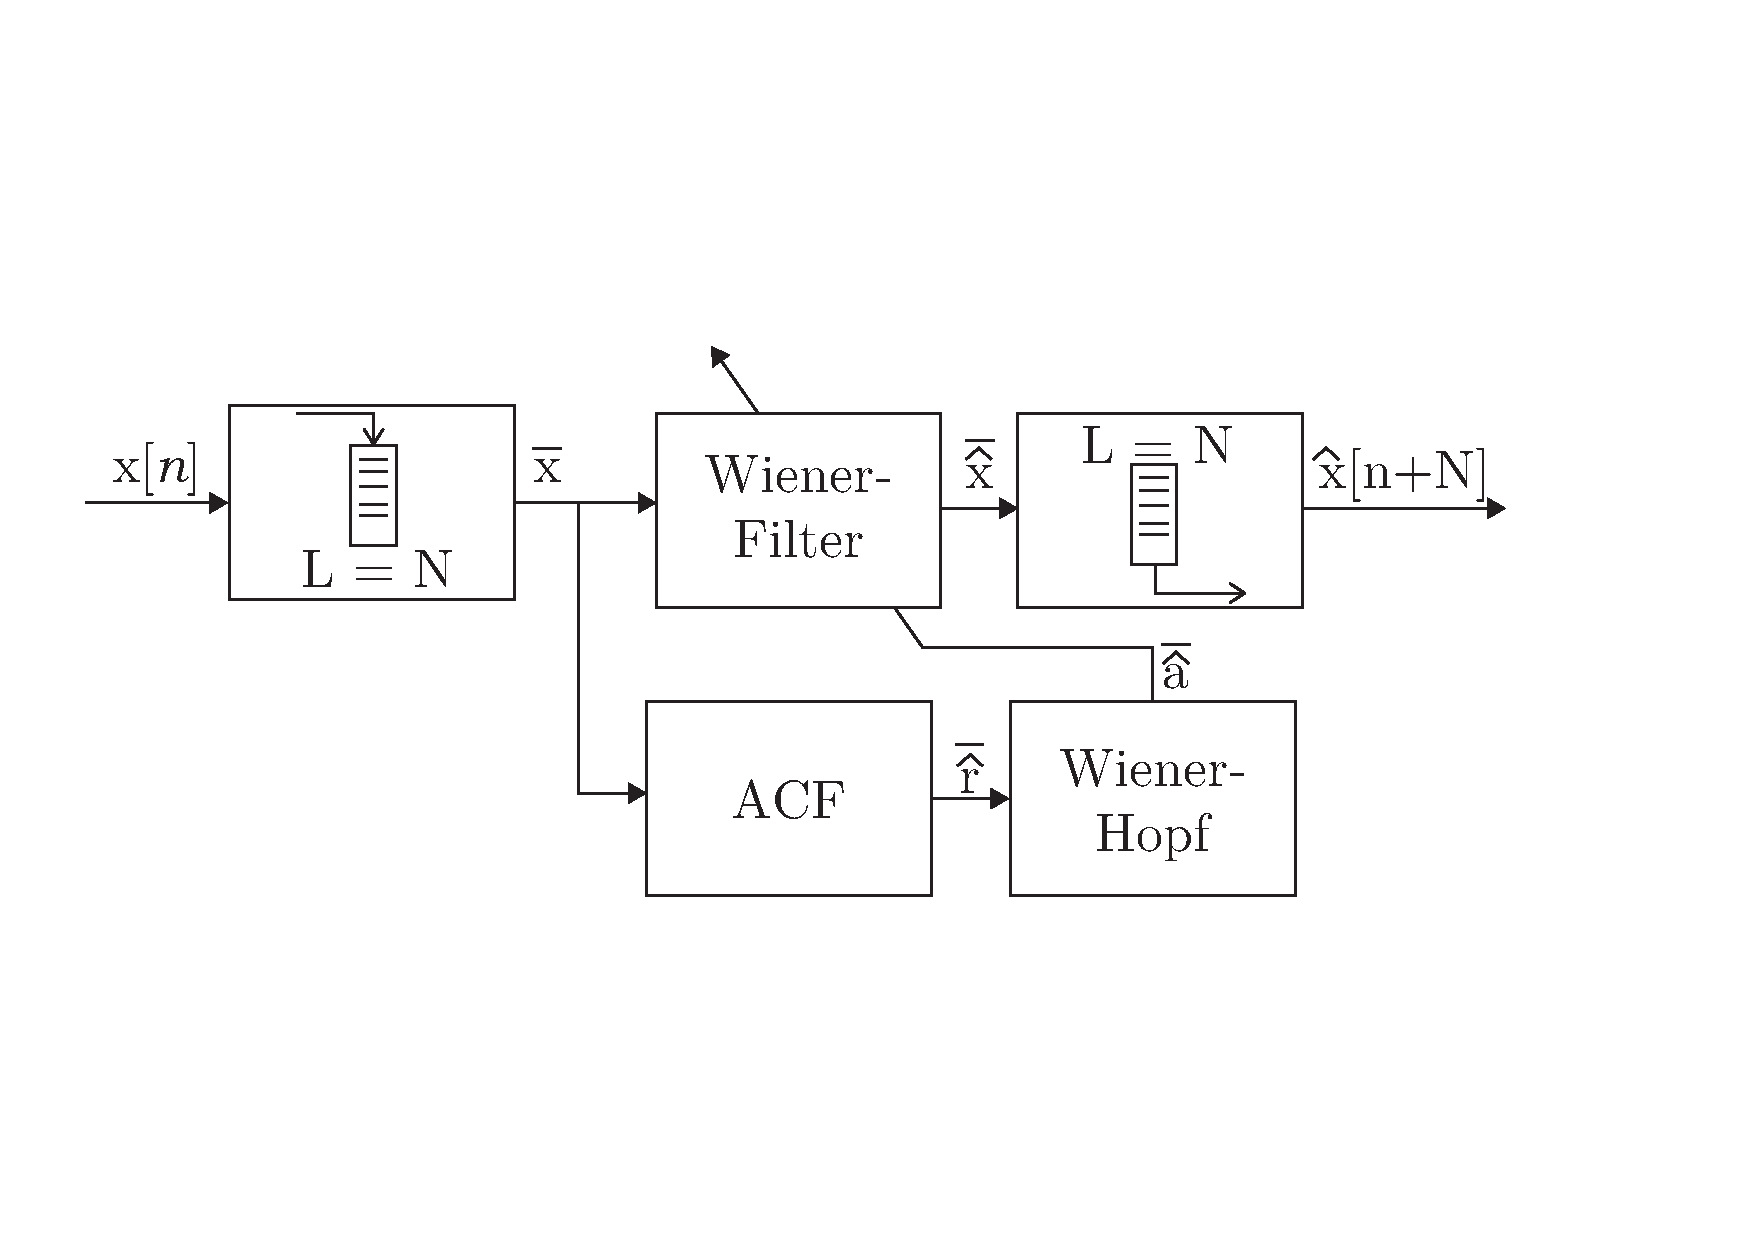
\includegraphics[width=\textwidth]{figures/WienerHopf}
			\end{figure}
%		$\hat{x}[n+P] =- \sum^{M-1}_{i=1}\hat{a}_i[n]x[(n+P)-i]$
		\end{column}
	\end{columns}
\end{frame}


\subsection{The algorithm}
\begin{frame}{Prediction}{Deriviations}
	\begin{columns}
		\begin{column}{0.45\textwidth}
			\begin{itemize}
				\item The Wiener filter 
				\vspace{3mm}
				\item The LPC found by minimizing 
				\vspace{3mm}
				\item The gradient $\frac{\partial E\{e^2[n]\}}{\partial a_k}$
				\vspace{3mm}
				\item With autocorrelations
				\vspace{3mm}
				\item Yielding Wiener Hopf				
			\end{itemize}
		\end{column}
		\begin{column}{0.55\textwidth} 
			\begin{itemize}
				\item[] $\hat{x}[n+P] =- \sum^{M-1}_{i=1}\hat{a}_i[n]x[(n+P)-i]$
				\vspace{3mm}
				\item[] $E\{e^2[n]\}=E\{(x[n]+\sum_{i=1}^{M}a_ix[n-i] )^2\}$
				\vspace{3mm}
				\item[] $2E\{(x[n]+\sum_{i=1}^{M}a_ix[n-i] )x[n-k]\}=0$
				\vspace{3mm}
				\item[] $r_x[k]+\sum_{i=1}^{M}a_iR_x[i-k]=0$
				\vspace{3mm}
				\item[] $R  \bar{a} = -\bar{r}_x$
			\end{itemize}		
		\end{column}
	\end{columns}
\end{frame}

\subsection{Predicted Speech}
\begin{frame}{Prediction}{Autocorrelation Function Estimation}
	\begin{columns}
		\begin{column}{0.5\textwidth}
			\begin{itemize}
				\item Frame based estimation of autocorrelation function, $\bar{\hat{r}}$
				\item Same  $\bar{\hat{r}}$ used for N-O samples
				\item Non-recursive
				\item Window function
			\end{itemize}
		\end{column}
		\begin{column}{0.5\textwidth} 
			$\hat{r}_x[l] = \sum^{N}_{n=\left| l\right|} x_l[n]w_l[N-n]$\\
			\vspace{5mm}
			Where: \\
			$x_l[n]=x[n]x[n-l]$ and $w_l[n]=w[n]w[n+l]$
		\end{column}
	\end{columns}
\end{frame}

\begin{frame}{Prediction}{Solving the Wiener Hopf}
	\begin{columns}
		\begin{column}{0.4\textwidth}
			\begin{itemize}
				\item Wiener Hopf equation $R  \bar{a} = -\bar{r}_x$
				\item By inversion $\bar{a} = -R^{-1} \bar{r}_x$
				\item Levinson Durbin to estimate LPCs 
				\item Three steps using symmetry
			\end{itemize}
			
		\end{column}
		\begin{column}{0.6\textwidth} 
				\resizebox{1.0\columnwidth}{!}{	
				% This file was created by matlab2tikz.
%
%The latest updates can be retrieved from
%  http://www.mathworks.com/matlabcentral/fileexchange/22022-matlab2tikz-matlab2tikz
%where you can also make suggestions and rate matlab2tikz.
%
\definecolor{mycolor1}{rgb}{0.00000,0.44700,0.74100}%
%
\begin{tikzpicture}

\begin{axis}[%
width=4.521in,
height=3.566in,
at={(0.758in,0.481in)},
scale only axis,
xmin=0,
xmax=1200,
xlabel={$\bar{a}$ coefficient number [samples]},
xmajorgrids,
ymin=-1,
ymax=1,
ylabel={Amplitude [$\cdot$]},
ymajorgrids,
axis background/.style={fill=white}
]
\addplot[ycomb,color=mycolor1,solid,mark=o,mark options={solid},forget plot] plot table[row sep=crcr] {%
1	1\\
2	-0.994591758753941\\
3	0.577598786054949\\
4	-0.56439937705\\
5	0.421642445797749\\
6	-0.455438791785392\\
7	0.353497610112228\\
8	-0.320411589796261\\
9	0.200748803699669\\
10	-0.216674438025256\\
11	0.0994623708053426\\
12	-0.0953821559245687\\
13	-0.00192463454294252\\
14	0.0159417673822501\\
15	-0.0979316786853175\\
16	-0.00541595925328035\\
17	0.0615882993639095\\
18	-0.0462445386332499\\
19	-0.00259921661656184\\
20	0.0183187210388263\\
21	0.069337068785506\\
22	-0.048094340367949\\
23	-0.0329894330889547\\
24	0.0631415442895705\\
25	-0.0990827999117296\\
26	0.0955256995322645\\
27	-0.0728005116882783\\
28	0.0813943174168925\\
29	0.00152398687779046\\
30	-0.0384978629284667\\
31	0.00410938700832798\\
32	0.0281951094612341\\
33	0.00289214982986916\\
34	-0.0104043398413269\\
35	0.0143401451721214\\
36	0.0233560323704767\\
37	-0.0873854539343842\\
38	0.00897080894214509\\
39	-0.00265867177116226\\
40	0.0233245333637109\\
41	-0.0545250388362693\\
42	0.143242970271281\\
43	-0.129640202444641\\
44	0.0718792912734971\\
45	-0.02163708417439\\
46	-0.0119179772934752\\
47	-0.0319316744239656\\
48	0.0407146404789066\\
49	0.0516984437480139\\
50	-0.0805650626463168\\
51	0.0370080565419153\\
52	0.0109416726527612\\
53	-0.0415562321002652\\
54	0.0453836600510892\\
55	0.010512058513926\\
56	-0.0306016209231027\\
57	0.00935833065387279\\
58	0.0268752457055463\\
59	-0.0352866195932614\\
60	0.0931852086305448\\
61	-0.0465204636034362\\
62	0.0149060196004793\\
63	-0.0441085640383083\\
64	0.0713960839252398\\
65	-0.0275845286808858\\
66	-0.0514839061081215\\
67	0.0168935978141285\\
68	0.130143384530439\\
69	-0.113429243373028\\
70	0.0840080057333667\\
71	-0.0323938343844307\\
72	-0.0721560411384755\\
73	0.0723933902705625\\
74	-0.0640111234209918\\
75	0.000720538415029199\\
76	0.0361921541848261\\
77	0.0574228010162397\\
78	-0.153420573471668\\
79	0.133767952033421\\
80	-0.163005015501723\\
81	0.151894198735404\\
82	-0.10952493925243\\
83	0.0639009269821086\\
84	0.0579898431444349\\
85	-0.147997151460233\\
86	0.09691849882515\\
87	-0.0801485831179214\\
88	0.0554428267540067\\
89	0.00397506534496763\\
90	-0.0189616263319564\\
91	0.0189324630292373\\
92	-0.047728091717674\\
93	-0.00356366820399812\\
94	0.011699923243651\\
95	-0.00246884437335544\\
96	0.00427337259544596\\
97	0.0258232559245371\\
98	-0.0196143067207088\\
99	-0.0332177828062122\\
100	-0.00481219291176322\\
101	0.0166694012892781\\
102	0.0319255344315652\\
103	0.00225002135640855\\
104	0.00497325576402391\\
105	-0.0582695927644983\\
106	-0.0213469847027379\\
107	0.0500141372588148\\
108	-0.0379091729871621\\
109	0.0801421113433513\\
110	-0.0488372836005625\\
111	0.0225798753466502\\
112	0.0118551644027015\\
113	-0.0878277692293887\\
114	0.151275166586598\\
115	-0.0988236140873601\\
116	0.0799476527957205\\
117	-0.00699031152522953\\
118	0.0577027154589308\\
119	-0.00619534141200983\\
120	-0.0628738058269005\\
121	0.00019214300948896\\
122	-0.0517195165116923\\
123	0.0759217224247446\\
124	-0.0158162244724907\\
125	0.0571946643625386\\
126	-0.136152284080801\\
127	0.16133722234627\\
128	-0.130190572330273\\
129	0.0219093593508329\\
130	0.0656072700539845\\
131	-0.0600140482296896\\
132	0.0517704795636846\\
133	-0.0880033694125722\\
134	0.00791880804256468\\
135	0.0482947056191926\\
136	-0.028149881203749\\
137	-0.0082331258358081\\
138	0.0465927563310379\\
139	-0.0198410446947263\\
140	-0.00412285194861921\\
141	-0.0289861780013429\\
142	-0.0225254883920958\\
143	0.160533883595855\\
144	-0.0645871358337341\\
145	-0.0121832966631922\\
146	0.0594484032941877\\
147	-0.040948547335065\\
148	-0.0409847592554223\\
149	-0.0267465772305415\\
150	0.0821724920529709\\
151	-0.010263032056471\\
152	-0.0703272350603023\\
153	-0.000514435220834072\\
154	-0.0157308203458403\\
155	0.00283552142971367\\
156	-0.0354494562049354\\
157	-0.0183711819044854\\
158	0.00991982809846574\\
159	0.0657175598740559\\
160	-0.0257548444836454\\
161	0.0377220325714377\\
162	-0.018410484265225\\
163	-0.0369298903841436\\
164	0.090946881306407\\
165	-0.0704841078382576\\
166	0.0512387862732918\\
167	0.0149499633772765\\
168	-0.0665488013857631\\
169	0.0153882861016907\\
170	-0.0327370456371672\\
171	0.0702889706653211\\
172	-0.099940831120591\\
173	0.0419922866428552\\
174	-0.110397780313374\\
175	0.0941937241629513\\
176	-0.0938655132632848\\
177	0.128235017802642\\
178	-0.0577756946167382\\
179	0.0223663646961162\\
180	-0.00784878822240164\\
181	-0.0137434796895568\\
182	0.0045569663418146\\
183	0.00233120836458548\\
184	0.0538707993912425\\
185	-0.00520246642682534\\
186	-0.0192328961399259\\
187	0.044910115460334\\
188	-0.0608213533530885\\
189	0.055590769924247\\
190	-0.131163474790352\\
191	0.140849274251148\\
192	-0.0658308741728146\\
193	0.0958996111176784\\
194	-0.0418463789714539\\
195	0.0276036776155724\\
196	-0.000960333151891491\\
197	0.0114087545340448\\
198	0.00972843179995531\\
199	0.0216818157948553\\
200	0.0195338936162499\\
201	-0.148214670679808\\
202	0.138669207702129\\
203	-0.15742689957961\\
204	0.0917001191539073\\
205	-0.0574510854269293\\
206	0.0719846053796392\\
207	-0.0857862267356553\\
208	0.0656678155352895\\
209	-0.103555863907688\\
210	0.137719576292085\\
211	-0.124921380270085\\
212	0.0186716860510489\\
213	0.0338137024409902\\
214	0.0232992443678164\\
215	0.0063631935481121\\
216	0.0020409165113081\\
217	-0.0693474216429584\\
218	0.0731684624965752\\
219	-0.0540585117923372\\
220	0.0507781659518992\\
221	-0.0323625509946324\\
222	-0.0688163583325244\\
223	0.0520890753077033\\
224	-0.0753499210573657\\
225	0.0171796113119313\\
226	0.107207433423329\\
227	0.047949538836208\\
228	-0.0625071371866804\\
229	-0.000421842578491261\\
230	0.0286771202490931\\
231	-0.0121045462781305\\
232	0.0167143711417602\\
233	-0.0440406638559747\\
234	0.103376690599148\\
235	-0.130951171293567\\
236	0.143833909182551\\
237	-0.117390264651519\\
238	0.121206243888458\\
239	-0.125687299971372\\
240	0.10851425875072\\
241	-0.0797195763445403\\
242	0.01503175825758\\
243	0.0128294376069021\\
244	0.0584503191220888\\
245	-0.106944238748511\\
246	0.0421911042946649\\
247	0.00807501372334317\\
248	0.0226762962044883\\
249	-0.116622453733351\\
250	0.110047204893937\\
251	-0.130364577208574\\
252	0.151507166215124\\
253	-0.104897204196464\\
254	0.103152758112482\\
255	-0.0884613444038021\\
256	0.104083655504344\\
257	-0.0605066141120985\\
258	0.0484872866020645\\
259	-0.0148088042832148\\
260	-0.0735801208059508\\
261	0.11451675908879\\
262	-0.0787132391682116\\
263	0.0948432118413696\\
264	-0.153722298303622\\
265	0.0779398644589118\\
266	-0.139084287920151\\
267	0.163121228166866\\
268	-0.138287506177466\\
269	0.0685586429659899\\
270	-0.0530332311671666\\
271	-0.0679859331672184\\
272	0.106505640987979\\
273	-0.0227286547924829\\
274	0.0605325012174638\\
275	-0.0427803618112489\\
276	0.00509465000342163\\
277	0.00810416144756333\\
278	-0.0086148329172193\\
279	-0.0630486440935299\\
280	0.0371359460715961\\
281	0.0177718931824994\\
282	0.0350319515000498\\
283	-0.0090469288996467\\
284	0.0218911839916876\\
285	0.0119545590195287\\
286	-0.00121152798177556\\
287	-0.106954725345469\\
288	0.0705764280830575\\
289	-0.0386122647638\\
290	0.0634661367836756\\
291	-0.0357265287582687\\
292	-0.084862844678495\\
293	0.0518782888858031\\
294	-0.0374375929831042\\
295	0.0448840821521976\\
296	-0.0133093525171007\\
297	-0.0291799857018554\\
298	0.004369606375156\\
299	0.0139612365561215\\
300	-0.0842096200814614\\
301	0.0878454358612622\\
302	0.039776700309496\\
303	0.0420874176000731\\
304	-0.0488302718649648\\
305	0.0070706126820314\\
306	0.0100785700960164\\
307	0.0399231690106655\\
308	0.0083510057219737\\
309	0.0362824001575184\\
310	-0.0149722004858308\\
311	0.0358952176166941\\
312	-0.0947513672891264\\
313	0.0787734693942181\\
314	-0.0505089232637748\\
315	0.0508771209266038\\
316	-0.0520508871115169\\
317	0.0432744059466576\\
318	-0.0766218570217173\\
319	0.00670449136609899\\
320	-0.0244981708217248\\
321	0.0218515868407121\\
322	0.0252900993134229\\
323	-0.00651058243301978\\
324	0.00493804028757679\\
325	0.00397491784819631\\
326	0.0240146652009265\\
327	-0.0512337289588452\\
328	0.0499855325630795\\
329	-0.0613590355806186\\
330	0.0632259440151208\\
331	-0.0398930054019486\\
332	-0.0215256621253038\\
333	-0.0128777761727099\\
334	0.102387548827178\\
335	-0.108973032217751\\
336	0.0849938304674245\\
337	-0.0691644569905992\\
338	0.0577568227198031\\
339	-0.0698959851235187\\
340	0.0171975045011261\\
341	-0.0293596602965314\\
342	0.0653022352083232\\
343	-0.0983991580825515\\
344	0.10643267143165\\
345	-0.0517493019206017\\
346	0.00544133065656936\\
347	-0.0783128961429032\\
348	0.0156671639667987\\
349	0.0185307489330729\\
350	0.0339270926730504\\
351	-0.119854619859643\\
352	0.104241344976127\\
353	-0.041531515564374\\
354	0.0125928574249033\\
355	0.0117470983667129\\
356	0.0101516927732082\\
357	0.0620384169574355\\
358	-0.0401463010383932\\
359	0.0710122587354712\\
360	-0.0401838546652975\\
361	0.0165508758151328\\
362	-0.0574218946545401\\
363	0.0658385863057588\\
364	-0.0453856292717864\\
365	0.105454125749929\\
366	-0.0493620176862142\\
367	-0.095937708902322\\
368	0.0111780023802828\\
369	0.0951936599348839\\
370	-0.0306543035193239\\
371	0.0137317460914137\\
372	-0.057631253992609\\
373	0.0747697190518594\\
374	-0.0389150251164382\\
375	-0.0273987863258326\\
376	0.0131379955373632\\
377	-0.000968751291597997\\
378	-0.00779941541045223\\
379	-0.0191870490640972\\
380	-0.0179386025659942\\
381	0.046962477039719\\
382	-0.0514823903602822\\
383	0.012121194042437\\
384	-0.00355228416112045\\
385	0.0579393064878035\\
386	-0.0278907544590494\\
387	-0.0215732795459176\\
388	0.00377331823196714\\
389	0.00037644500403845\\
390	0.120125087915969\\
391	-0.0434613708743838\\
392	0.0173069848793213\\
393	-0.0133135388459715\\
394	-0.032947825936481\\
395	-0.0333930152409397\\
396	0.0139390540437955\\
397	0.0137966587579972\\
398	0.0133239952677924\\
399	-0.0581721764492386\\
400	0.0111304321658762\\
401	0.0798047277779017\\
402	-0.0589865282799599\\
403	0.0121920512131945\\
404	-0.00347264325816427\\
405	0.0209842318694193\\
406	-0.0511597507592163\\
407	-0.00489623506629369\\
408	0.0314224579890911\\
409	-0.0790628607806701\\
410	0.034686570680361\\
411	-0.00460775040364969\\
412	0.0353378472286446\\
413	-0.0284478819009528\\
414	-0.0395850606240033\\
415	0.0217757545470208\\
416	0.00686737534397768\\
417	0.0038234983007447\\
418	0.000546820146599772\\
419	0.0406616307423641\\
420	-0.0392865260416695\\
421	0.0908193699270829\\
422	-0.0407633712100486\\
423	0.00468514673797538\\
424	0.026684640144525\\
425	0.0107823006842059\\
426	-0.0104557169679367\\
427	-0.010056753974244\\
428	0.0196760298647226\\
429	-0.057670799802637\\
430	0.0339847990018909\\
431	-0.0295354282191139\\
432	0.0507698017107052\\
433	0.00963137947530546\\
434	-0.0681782857457186\\
435	0.0544819999007855\\
436	-0.00132851983035051\\
437	-0.0553289035665201\\
438	0.0252328105790669\\
439	-0.0701355081480003\\
440	0.0650860878880106\\
441	0.000310105082815904\\
442	-0.0728393452926293\\
443	0.0276935936408187\\
444	-0.0116123075612343\\
445	0.0691697267984792\\
446	-0.0539377909865564\\
447	0.0056074380234831\\
448	-0.0652646680027753\\
449	0.147195725008078\\
450	-0.159633753364835\\
451	0.175725173012503\\
452	-0.129469563584885\\
453	0.138805897655987\\
454	-0.147300759569996\\
455	0.0953064290226151\\
456	-0.0417025226218452\\
457	0.0210496968008243\\
458	-0.0516872151692684\\
459	0.0225168586176128\\
460	0.00826138120448795\\
461	-0.0123173546637078\\
462	-0.00424305771714604\\
463	-0.00713872048167795\\
464	-0.00741467574754975\\
465	0.032716713394156\\
466	-0.0202715509003741\\
467	0.0304796253811115\\
468	0.0147798087354226\\
469	-0.0478287849270069\\
470	0.00441888629533686\\
471	0.0440984899657229\\
472	-0.0309971266068397\\
473	0.0513689438878582\\
474	-0.0284624475918838\\
475	-0.00119887624423535\\
476	0.00913977301230825\\
477	-0.0105757691802577\\
478	-0.00360190486190397\\
479	0.0239230689823852\\
480	-0.0266952225211406\\
481	0.0497835931238531\\
482	-0.0808864960479051\\
483	0.0805999136751352\\
484	-0.0183077567015436\\
485	-0.0181956254598689\\
486	-0.0181517546623945\\
487	0.0493816170367165\\
488	-0.0180009163086466\\
489	0.00543094581314977\\
490	-0.0673301956545904\\
491	0.0644627922586518\\
492	-0.0403395903370941\\
493	0.0221724588320436\\
494	0.0356938811106471\\
495	-0.0362975203762051\\
496	-0.00212709083976482\\
497	-0.0241478507235664\\
498	0.0142623382302589\\
499	0.0326062984276708\\
500	-0.0255431036303682\\
501	0.000719899211520579\\
502	0.0338197984802382\\
503	-0.0450756354617997\\
504	0.0466477275194661\\
505	-0.0481473822640161\\
506	0.00195152871366411\\
507	-0.0491493624825422\\
508	0.106452649278221\\
509	-0.0957644658016058\\
510	0.026540860031506\\
511	-0.0393982275742373\\
512	0.0543535123771766\\
513	-0.0684333357195146\\
514	0.0531469100615362\\
515	-0.0187218906224607\\
516	0.0509155971989691\\
517	-0.0676410268145459\\
518	0.0779975579709987\\
519	-0.00674415573687235\\
520	-0.0359203832905507\\
521	0.0290050362219559\\
522	-0.0919617605228787\\
523	0.0566679303487076\\
524	-0.0292182962140174\\
525	0.0360073573348965\\
526	-0.0860200337188611\\
527	0.0627652758114096\\
528	-0.0223579099622297\\
529	0.0238868117865841\\
530	-0.070767130283142\\
531	0.0827333823871957\\
532	-0.0118970412732456\\
533	0.00670450402985189\\
534	0.0360685208574608\\
535	-0.0146593080009682\\
536	-0.00821507412453001\\
537	0.0138582115953955\\
538	-0.0409074935456772\\
539	0.0463495769490292\\
540	-0.0271416230944834\\
541	0.0150784048682119\\
542	-0.019995844685109\\
543	0.0385070138021411\\
544	-0.0495156703921054\\
545	0.0149166678850766\\
546	-0.00192858642638111\\
547	0.011434844974249\\
548	0.0040535477712356\\
549	-0.0253521543571308\\
550	0.0617147069268947\\
551	-0.00997227411447382\\
552	0.0247951039972557\\
553	-0.0215851201890278\\
554	0.0571376958296452\\
555	-0.0787968182305311\\
556	0.0826969062666243\\
557	-0.082452610732155\\
558	0.0796749934059455\\
559	-0.0597949844825403\\
560	0.0644931049079143\\
561	-0.0116363195567097\\
562	0.0318892658106936\\
563	-0.0420347744613139\\
564	0.045738970775581\\
565	-0.0628383758949566\\
566	0.0219756105090976\\
567	-0.0180599868623234\\
568	0.0107754556162708\\
569	0.0038025225096497\\
570	-0.00870267857827281\\
571	-0.0197440265871929\\
572	0.0016236324122219\\
573	-0.0492399146755611\\
574	0.0357406713428304\\
575	-0.0119954805679857\\
576	-0.0535295887371167\\
577	0.024474945322212\\
578	-0.015051416189548\\
579	0.0660335373444352\\
580	-0.110928674764192\\
581	0.0854713155902536\\
582	-0.0404600643647783\\
583	0.0378012887188011\\
584	-0.0385464063229996\\
585	0.0582340075886005\\
586	-0.0508370275262393\\
587	0.029755247560839\\
588	-0.0210361418692438\\
589	0.00497810617332319\\
590	-0.0302509706117435\\
591	0.046552021650895\\
592	-0.0343158652155814\\
593	-0.0217077037647881\\
594	0.0153665211005116\\
595	0.020193956756541\\
596	-0.00942855594933917\\
597	-0.00186008390304274\\
598	0.0409958831715225\\
599	-0.0265301688041334\\
600	0.020963585696271\\
601	-0.0541513803998359\\
602	0.0728339084450719\\
603	-0.0765492137749079\\
604	0.0420187173776001\\
605	-0.0664854755016608\\
606	0.0595804986423111\\
607	-0.0495150557267548\\
608	0.0278350404257809\\
609	-0.0273017633935807\\
610	0.0708309567134807\\
611	-0.0321530759862225\\
612	0.00633173410164845\\
613	-0.00262701630474092\\
614	0.0251402954283222\\
615	0.0133846270181137\\
616	0.0372362684443319\\
617	-0.00437615986630789\\
618	-0.020288358332762\\
619	0.0166408282297159\\
620	0.0318585753973898\\
621	-0.0327657180542348\\
622	-0.00745432528318361\\
623	-0.00674797930387199\\
624	-0.0335738237835694\\
625	0.0191656507834491\\
626	0.0202211647703701\\
627	-0.0165986347929733\\
628	0.00284804110332755\\
629	-0.0282271750850931\\
630	0.0315776641570291\\
631	-0.0142538803862378\\
632	-0.00534786321831858\\
633	0.010903390914613\\
634	-0.0109571714857418\\
635	-0.0125412247497939\\
636	-0.00999327528481255\\
637	0.0451879238205745\\
638	-0.0517667287275266\\
639	0.0489328260802429\\
640	-0.0820657534434935\\
641	0.0790430785660349\\
642	-0.0226692571641762\\
643	0.0326404510180052\\
644	-0.0108407433990884\\
645	-0.00899214959197648\\
646	0.00830897878562586\\
647	0.000946627048972462\\
648	0.0185734069710903\\
649	-0.0564755486352752\\
650	0.0570670500775488\\
651	-0.0385871877751491\\
652	-0.0199227640854179\\
653	-0.0318291022459721\\
654	0.0553758318691506\\
655	-0.0200788659830637\\
656	-0.0738385341541563\\
657	0.0577833025271774\\
658	-0.000122930600699644\\
659	0.0150006442560763\\
660	-0.0404920690885755\\
661	0.0287269930843718\\
662	0.013947023937647\\
663	0.0081578254962504\\
664	-0.0158975758902922\\
665	0.000323748126493025\\
666	-0.00272961646017427\\
667	0.0363547222386558\\
668	-0.0518175214869233\\
669	0.0301967022374721\\
670	-0.00873771011950624\\
671	0.0357462808656627\\
672	-0.0132675430319018\\
673	0.0116542565889896\\
674	0.00563352223346816\\
675	0.00562341358047697\\
676	0.0071817394795698\\
677	-0.00737628788886673\\
678	0.0424043288682645\\
679	-0.0162336083932693\\
680	-0.00867832744254697\\
681	-0.0211794112310524\\
682	0.00983729197779023\\
683	-0.0109614037189236\\
684	-0.0073765008343268\\
685	0.0176763685061172\\
686	-0.0179059492920596\\
687	-0.00179722614964541\\
688	0.00513274292490498\\
689	-0.0448664311522044\\
690	0.0491972623400637\\
691	-0.0582523506838497\\
692	0.0813652139410268\\
693	-0.0528470436883339\\
694	0.0203739616326228\\
695	-0.0338640508711242\\
696	0.03612043049885\\
697	-0.0368762992558337\\
698	0.0776689474163389\\
699	-0.07593406608569\\
700	0.0512316584057675\\
701	-0.0507197458195959\\
702	0.049420941410984\\
703	-0.00642986126307438\\
704	-0.0302045391683323\\
705	-0.0122456065129866\\
706	0.0224220451020372\\
707	-0.00767187450520878\\
708	-0.00540581904458004\\
709	0.00752953003683826\\
710	-0.00720531799268049\\
711	0.0242515259022448\\
712	-0.0525700166911495\\
713	0.0639383066538936\\
714	-0.0469328738048739\\
715	0.0128311074969418\\
716	-0.0150714165709426\\
717	0.0316095911787001\\
718	-0.00439942609557501\\
719	-0.00412366673849182\\
720	-0.00958638108445356\\
721	-0.0332990304478933\\
722	0.0517578075270149\\
723	-0.0708306342310677\\
724	0.0570896118073768\\
725	-0.0418502358726303\\
726	0.0730956094528063\\
727	-0.0647966958531\\
728	0.0744597477979558\\
729	-0.0390416319715168\\
730	0.0175500916771034\\
731	-0.0215000536115363\\
732	-0.00984999617441447\\
733	0.0111457677660351\\
734	0.0296989358665805\\
735	-0.0418656447295905\\
736	0.0186616778884763\\
737	-0.0182716552818162\\
738	0.0452474522698643\\
739	-0.0287423664999409\\
740	0.0180596952659249\\
741	-0.050348903334055\\
742	0.0418500131501951\\
743	-0.0317128824417503\\
744	0.0325042401793216\\
745	0.0275817341762817\\
746	-0.00374317125537519\\
747	0.00333728744297942\\
748	-0.00266360333480387\\
749	-0.0194095924339113\\
750	0.00718698816197052\\
751	0.00123530413616584\\
752	-0.0289130853892944\\
753	0.015659388277974\\
754	-0.000956148918618391\\
755	-0.0118159950963628\\
756	0.0171337248969425\\
757	0.0147653648124708\\
758	-0.0298797973560674\\
759	0.0163224087663343\\
760	0.0109594493583532\\
761	0.00280358114132781\\
762	-0.053342681811054\\
763	0.0301594082852892\\
764	-0.0520681792592812\\
765	0.0491729445992624\\
766	-0.0367216796803345\\
767	0.00624220947208129\\
768	0.00452594430285254\\
769	-0.000774860887718465\\
770	-0.000473255683175891\\
771	-0.0463578818513603\\
772	-0.00457483097963132\\
773	0.0252946337418936\\
774	0.0194681393237065\\
775	0.00360089210252186\\
776	0.00193335369048394\\
777	-0.00187962939056703\\
778	-0.00307502080984488\\
779	0.00436907425129862\\
780	0.0116319409364824\\
781	0.00172994862399518\\
782	-0.0241997163151364\\
783	-0.00350917786665283\\
784	-0.00271697210160523\\
785	0.0184115093510247\\
786	0.0315669838432786\\
787	-0.0479075680579089\\
788	0.0437350270725782\\
789	0.0312761538491122\\
790	-0.0215141235014767\\
791	0.00999509367091622\\
792	0.0122713737374134\\
793	-0.00202132653722777\\
794	0.00669274820541701\\
795	-0.00677918871498885\\
796	0.0037687846438644\\
797	-0.0132603558395184\\
798	-0.00662591143941919\\
799	-0.0176684562270708\\
800	0.0220412546186826\\
801	-0.000136745253828028\\
802	-0.0282907088048622\\
803	0.00624288615966217\\
804	0.00318089178213014\\
805	0.0143221458744211\\
806	-0.0369026010705914\\
807	0.0346173141471226\\
808	-0.000461956206963505\\
809	0.0309820937915094\\
810	-0.0531129841164972\\
811	0.0176051746781473\\
812	0.00099574357519702\\
813	-0.00402482182729862\\
814	0.0419887046090053\\
815	-0.0314144645920401\\
816	0.0323396331026378\\
817	-0.0254679237325095\\
818	0.0152575757219925\\
819	-0.0240834734471913\\
820	-0.00140097334322912\\
821	0.0154492490889067\\
822	-0.0192069984034073\\
823	0.00641635902606211\\
824	-0.0279695423285002\\
825	0.0549390907273722\\
826	-0.0491174087073567\\
827	0.0246481690745413\\
828	-0.0231846279357837\\
829	0.000538903508043818\\
830	-0.00866802293501658\\
831	-0.0284981795440872\\
832	0.0250478197655098\\
833	0.0104615195832797\\
834	-0.0337536974110904\\
835	0.0636202487064761\\
836	-0.0424746802363534\\
837	0.0288241921264162\\
838	-0.05929765734931\\
839	0.0523748346554357\\
840	-0.0463101531621142\\
841	0.0593080996028237\\
842	-0.0412396850963799\\
843	0.0363981710529421\\
844	-0.0489868869311608\\
845	0.0620035905076325\\
846	-0.0559578924770217\\
847	0.0097335202782351\\
848	-0.00963396748629084\\
849	-0.00316454573075891\\
850	0.00859832903653729\\
851	0.0019798892381916\\
852	-6.17482101540213e-05\\
853	0.0327803205117327\\
854	-0.0627867828132602\\
855	0.035907286448238\\
856	0.0203172334835491\\
857	-0.00603360598069843\\
858	0.00739471739838771\\
859	-0.0346010708621581\\
860	0.03323907103731\\
861	-0.0295837540275744\\
862	0.0418010445000609\\
863	-0.0207507287518364\\
864	0.0349653533627438\\
865	-0.0540489841295945\\
866	0.0340979311863961\\
867	-0.0188079443966586\\
868	0.029715507086209\\
869	-0.00974954387971257\\
870	0.0126849986831171\\
871	-0.01037677287173\\
872	0.00838080032633218\\
873	-0.0280328537664732\\
874	0.0356871149848888\\
875	-0.0358109725805833\\
876	0.0588654099703202\\
877	-0.0337290519540291\\
878	0.000555899518926698\\
879	-0.0312322974459565\\
880	0.0159398700065158\\
881	-0.00883347990711795\\
882	0.0128113190270583\\
883	0.00978382158706357\\
884	-0.019581797679996\\
885	0.0287262874592036\\
886	-0.0178390632574561\\
887	-0.0127521225643336\\
888	0.0292451474021201\\
889	-0.0238703217483263\\
890	0.00423093593531149\\
891	0.00169937722325111\\
892	-0.000530547346951588\\
893	0.00195427702934337\\
894	-0.0156272310203671\\
895	0.0383550653010517\\
896	-0.0486991695033621\\
897	0.043047778621131\\
898	-0.0379225706449383\\
899	0.0426196180417181\\
900	-0.0578764288056092\\
901	0.0431936908142343\\
902	-0.0452887223068303\\
903	0.0423934177143018\\
904	-0.0159357697556157\\
905	0.0302115264996364\\
906	-0.0190365938451044\\
907	-0.0292800447479092\\
908	0.0345606501144436\\
909	-0.0384789999182685\\
910	0.0305767991397613\\
911	-0.0312374885443696\\
912	0.016178991978654\\
913	-0.0305307668192185\\
914	0.0199739310301558\\
915	0.0068789707912395\\
916	0.00421295341906864\\
917	-0.00273973516122845\\
918	0.0232610104758675\\
919	-0.0175057184333827\\
920	0.0105941936586144\\
921	-0.0152634271290262\\
922	0.0200686050086839\\
923	0.00760038549230898\\
924	-0.0035730310558606\\
925	-0.0151187941962728\\
926	0.0222962445352178\\
927	-0.0243040877659024\\
928	0.0245495399264401\\
929	-0.0242222058991696\\
930	-0.0170304047930469\\
931	0.0393084989360171\\
932	-0.0282020336564638\\
933	0.0363889506130912\\
934	-0.0321928922947534\\
935	0.0325852912220226\\
936	-0.038961680911756\\
937	0.00430853498177152\\
938	0.00892902533852016\\
939	0.0161034226560361\\
940	-0.0417590412739406\\
941	0.0387870990973694\\
942	-0.0403527716805962\\
943	0.0524868762499622\\
944	-0.0392898226954932\\
945	0.0293309058037116\\
946	-0.0252361207676451\\
947	0.0134183507026237\\
948	-0.0352301006850478\\
949	0.0408749138149086\\
950	-0.0281694065172554\\
951	0.0423954900743229\\
952	-0.0109990570054637\\
953	0.0108017369217237\\
954	-0.00890651551218709\\
955	-0.0049927889952978\\
956	-0.0104403970174828\\
957	0.00515075593893111\\
958	-0.00438337844302079\\
959	0.0139916849529477\\
960	-0.018549170817036\\
961	0.00613056238100708\\
962	-0.013052096663449\\
963	-0.00547433918513581\\
964	-0.00348861097009431\\
965	0.0032169213759755\\
966	-0.00618949118497405\\
967	-0.00479831429525458\\
968	0.0110321604434085\\
969	-0.00655130644910457\\
970	-0.00365197137072742\\
971	0.0276774713091008\\
972	-0.0163022858387408\\
973	0.0158618184006027\\
974	-0.0033208502876716\\
975	0.0193786270286632\\
976	-0.0258884951604846\\
977	0.00302211175055806\\
978	0.00946445796642215\\
979	0.00964568884810295\\
980	-0.0136107490332863\\
981	0.00860287349470504\\
982	0.0240532841682108\\
983	-0.01324823094495\\
984	0.00894679806281261\\
985	-0.00461745111148915\\
986	0.0127096381868461\\
987	-0.0158367556097859\\
988	0.0215996366880664\\
989	-0.0312478107850228\\
990	0.00255362207908951\\
991	0.00452924694931108\\
992	-0.0037653552005129\\
993	-0.00713082349102382\\
994	-0.000737779828488692\\
995	0.00158919035591667\\
996	-0.0188607057841491\\
997	-0.0187885369020253\\
998	0.0243433258633772\\
999	-0.00724334636528078\\
1000	0.0219198528322448\\
1001	-0.0211261889874035\\
1002	0.0238898574489123\\
1003	-0.0202230195626497\\
1004	0.00581831272557549\\
1005	-0.00940633526365786\\
1006	0.0234079425540169\\
1007	-0.0221769272256902\\
1008	0.00650582049833641\\
1009	0.00545262901141742\\
1010	-0.0125828318971165\\
1011	0.0187362216793242\\
1012	-0.00805618535813062\\
1013	-0.0128648824165884\\
1014	0.0156811708794454\\
1015	-0.0297234274549779\\
1016	0.028342354318898\\
1017	-0.0234430585582658\\
1018	0.0228079332238132\\
1019	-0.00551445540737194\\
1020	-0.00300898830550356\\
1021	0.00113070101765042\\
1022	-0.00501425048073887\\
1023	0.0106481972150537\\
1024	-0.0242023616523245\\
1025	0.00216244106528927\\
1026	0.0067216654588569\\
1027	0.0183051114003929\\
1028	-0.012251731050116\\
1029	0.00825167236576373\\
1030	-0.00538122657576703\\
1031	0.00976392719719372\\
1032	0.0127245447957808\\
1033	-0.0178598436329853\\
1034	0.0212015113524563\\
1035	0.00419607535183782\\
1036	-0.00995674405534504\\
1037	7.3591071114733e-05\\
1038	-0.0168181773209058\\
1039	-0.00382803680671203\\
1040	0.0162048435795386\\
1041	-0.00109646753731559\\
1042	0.00685871030177621\\
1043	-0.0116241859250228\\
1044	0.0126046282399291\\
1045	-0.019399344625517\\
1046	0.0307691971588243\\
1047	-0.0255618142912725\\
1048	0.0360254178700626\\
1049	-0.0253735449167109\\
1050	0.0127673603659884\\
1051	0.00143391739352072\\
1052	0.0028424653069407\\
1053	-0.0253782041981463\\
1054	0.012386954562051\\
1055	0.000538313788752792\\
1056	-0.0197082689218648\\
1057	0.00295306672777955\\
1058	0.00945645347908047\\
1059	-0.00683510159307132\\
1060	-0.0135756554847812\\
1061	0.022918333678974\\
1062	0.000286889991591173\\
1063	-0.0142695155142981\\
1064	0.013633570265193\\
1065	0.00028871267122874\\
1066	-0.0141442791426039\\
1067	0.00578427646380267\\
1068	-0.00203310167121267\\
1069	0.00947296165660878\\
1070	-0.00265358687334065\\
1071	0.0078161993813875\\
1072	-0.0122492722943016\\
1073	-0.00704841699979238\\
1074	0.00529882875539858\\
1075	0.00275953130535444\\
1076	0.00637618604830904\\
1077	-0.00881197327550071\\
1078	0.0100625645631697\\
1079	-0.0256312634299176\\
1080	0.0106049188683194\\
1081	-0.0104204814739522\\
1082	0.0065908170155135\\
1083	-0.000649237500603224\\
1084	-0.00960984843392509\\
1085	-0.0047436464109978\\
1086	-0.00400108522284857\\
1087	0.01256930831739\\
1088	-0.0114848988984839\\
1089	0.00955598417959302\\
1090	0.00482087134149575\\
1091	-0.0139512414734315\\
1092	0.0179214131334099\\
1093	-0.0154881064035462\\
1094	0.0197762980300765\\
1095	-0.022655120251454\\
1096	0.0283698455801697\\
1097	-0.0159126587217749\\
1098	0.0102609248913223\\
1099	0.0207227278870287\\
1100	-0.0319880183007665\\
1101	0.0207351440961826\\
1102	0.00720432851581276\\
1103	0.00340901117233287\\
1104	-0.0216086240560661\\
1105	0.0149649971190504\\
1106	-0.0184161283310275\\
1107	0.0191471989520794\\
1108	-0.0107552231608101\\
1109	0.0175149683473083\\
1110	-0.0168114683331127\\
1111	0.0071213519615582\\
1112	0.000202487619050836\\
1113	0.00519871810853792\\
1114	-0.014840643281482\\
1115	0.0293841523190201\\
1116	-0.0276039956493116\\
1117	0.0241789225082128\\
1118	-0.00982170139184777\\
1119	0.00421841511651009\\
1120	-0.00740501650436087\\
1121	0.00142204381831969\\
1122	-0.0123951070711822\\
1123	0.00746710133510213\\
1124	-0.00552531425738575\\
1125	0.00715599742289863\\
1126	-0.0143912303130903\\
1127	0.00688024109362778\\
1128	0.000593660130952126\\
1129	0.00313907103879587\\
1130	-0.00104456068253942\\
1131	-0.00108081328214624\\
1132	-0.00178360844395912\\
1133	0.00799064163374835\\
1134	0.00422319778624363\\
1135	-0.01913210110103\\
1136	0.010457464165564\\
1137	0.00744443209758379\\
1138	0.00633180666493367\\
1139	-0.0311290750298423\\
1140	0.0244437538763703\\
1141	-0.0272738801533201\\
1142	0.0179351779229655\\
1143	-0.00968627974654913\\
1144	0.00265614091560291\\
1145	-0.00562832138018484\\
1146	0.0109143573623085\\
1147	-0.0010759609861369\\
1148	0.00815576009968903\\
1149	-0.013663826252326\\
1150	0.0138343062941092\\
1151	-0.00949055421188429\\
1152	0.010359381861337\\
1153	-0.0169549626550402\\
1154	0.00747995686405338\\
1155	-0.0121482945812986\\
1156	-0.0139900027767546\\
1157	0.0262650818705108\\
1158	-0.00500469425749369\\
1159	0.0098944415316764\\
1160	-0.0159917506093891\\
1161	0.00801906130915617\\
1162	-0.0159506665420222\\
1163	0.00971168146665251\\
1164	-0.00555991925219493\\
1165	0.0147216055261804\\
1166	0.00156917780232382\\
1167	-0.0191004855322896\\
1168	0.0247154956646975\\
1169	-0.0242621690791319\\
1170	0.0305960958301988\\
1171	-0.0210367885714712\\
1172	0.0239789021329863\\
1173	-0.0322670592723956\\
1174	0.0255791440470841\\
1175	-0.0144727930124926\\
1176	0.0148615207130552\\
1177	-0.00346831867191282\\
1178	0.0198585159254037\\
1179	-0.0120113300584643\\
1180	0.0115109180947089\\
1181	-0.0228350771345229\\
1182	0.0132422101703677\\
1183	-0.0198485864068885\\
1184	0.0133212034412912\\
1185	-0.0193453201981531\\
1186	0.0209610511957775\\
1187	-0.0283838272938284\\
1188	0.0239183922283217\\
1189	-0.014757168781136\\
1190	0.015838398308597\\
1191	-0.0169356797806228\\
1192	0.000131510010547939\\
1193	0.00863648152175282\\
1194	-0.0117691096881496\\
1195	0.0128697277373532\\
1196	-0.00163702228635144\\
1197	-0.00324355035296205\\
1198	0.00326674399515191\\
1199	-0.00825073399829394\\
1200	0.010006109277578\\
};
\end{axis}
\end{tikzpicture}%
			}	
		\end{column}
	\end{columns}
\end{frame}

\begin{frame}{Prediction}{A Predicted Signal}
	\begin{columns}
		\begin{column}{0.4\textwidth}
			\begin{itemize}
				\item[\textcolor{MATLABblue}{---}] Speech signal
				\item[\textcolor{MATLABorange}{---}] Predicted speech signal
				\item N = 1200 samples
				\item O = 1100 samples
				\item P = 10 samples
				\item $f_s$ = 48000 Hz
			\end{itemize}
			
		\end{column}
		\begin{column}{0.6\textwidth} 
			\resizebox{1.0\columnwidth}{!}{	
				% This file was created by matlab2tikz.
%
%The latest updates can be retrieved from
%  http://www.mathworks.com/matlabcentral/fileexchange/22022-matlab2tikz-matlab2tikz
%where you can also make suggestions and rate matlab2tikz.
%
\definecolor{mycolor1}{rgb}{0.00000,0.44700,0.74100}%
\definecolor{mycolor2}{rgb}{0.85000,0.32500,0.09800}%
%
\begin{tikzpicture}

\begin{axis}[%
width=4.521in,
height=3.566in,
at={(0.758in,0.481in)},
scale only axis,
xmin=0,
xmax=1200,
xlabel={samplenumber [samples]},
xmajorgrids,
ymin=-0.2,
ymax=0.2,
ylabel={Amplitude [$\cdot$]},
ymajorgrids,
axis background/.style={fill=white}
]
\addplot [color=mycolor1,solid,forget plot]
  table[row sep=crcr]{%
1	0.10540771484375\\
2	0.107025146484375\\
3	0.10467529296875\\
4	0.100128173828125\\
5	0.097076416015625\\
6	0.09136962890625\\
7	0.088134765625\\
8	0.085235595703125\\
9	0.08026123046875\\
10	0.07720947265625\\
11	0.0726318359375\\
12	0.068939208984375\\
13	0.068389892578125\\
14	0.067962646484375\\
15	0.06634521484375\\
16	0.06512451171875\\
17	0.064483642578125\\
18	0.065704345703125\\
19	0.06829833984375\\
20	0.068756103515625\\
21	0.068634033203125\\
22	0.067352294921875\\
23	0.06280517578125\\
24	0.0589599609375\\
25	0.05645751953125\\
26	0.053009033203125\\
27	0.048828125\\
28	0.043914794921875\\
29	0.039215087890625\\
30	0.03631591796875\\
31	0.0338134765625\\
32	0.032135009765625\\
33	0.03131103515625\\
34	0.028656005859375\\
35	0.0260009765625\\
36	0.025726318359375\\
37	0.02642822265625\\
38	0.026214599609375\\
39	0.0257568359375\\
40	0.0250244140625\\
41	0.021636962890625\\
42	0.0184326171875\\
43	0.014007568359375\\
44	0.008819580078125\\
45	0.00555419921875\\
46	-0.00054931640625\\
47	-0.0059814453125\\
48	-0.0087890625\\
49	-0.013153076171875\\
50	-0.016510009765625\\
51	-0.018798828125\\
52	-0.019378662109375\\
53	-0.0189208984375\\
54	-0.019683837890625\\
55	-0.020782470703125\\
56	-0.02008056640625\\
57	-0.018463134765625\\
58	-0.01776123046875\\
59	-0.016937255859375\\
60	-0.0164794921875\\
61	-0.016754150390625\\
62	-0.0186767578125\\
63	-0.02130126953125\\
64	-0.021209716796875\\
65	-0.021026611328125\\
66	-0.0218505859375\\
67	-0.023468017578125\\
68	-0.024322509765625\\
69	-0.022125244140625\\
70	-0.019256591796875\\
71	-0.0169677734375\\
72	-0.014556884765625\\
73	-0.010772705078125\\
74	-0.0078125\\
75	-0.005889892578125\\
76	-0.00140380859375\\
77	0.003173828125\\
78	0.006988525390625\\
79	0.00933837890625\\
80	0.009735107421875\\
81	0.012176513671875\\
82	0.013702392578125\\
83	0.012847900390625\\
84	0.0123291015625\\
85	0.011474609375\\
86	0.01171875\\
87	0.0113525390625\\
88	0.011199951171875\\
89	0.01300048828125\\
90	0.014556884765625\\
91	0.015960693359375\\
92	0.01763916015625\\
93	0.018157958984375\\
94	0.019561767578125\\
95	0.02227783203125\\
96	0.02276611328125\\
97	0.02410888671875\\
98	0.026702880859375\\
99	0.025543212890625\\
100	0.02471923828125\\
101	0.02508544921875\\
102	0.023529052734375\\
103	0.022003173828125\\
104	0.019744873046875\\
105	0.017364501953125\\
106	0.0167236328125\\
107	0.0169677734375\\
108	0.018341064453125\\
109	0.0201416015625\\
110	0.022552490234375\\
111	0.024169921875\\
112	0.024169921875\\
113	0.027099609375\\
114	0.030670166015625\\
115	0.03125\\
116	0.0333251953125\\
117	0.036834716796875\\
118	0.03778076171875\\
119	0.03802490234375\\
120	0.039947509765625\\
121	0.041351318359375\\
122	0.041290283203125\\
123	0.0411376953125\\
124	0.040863037109375\\
125	0.040740966796875\\
126	0.041961669921875\\
127	0.043243408203125\\
128	0.044525146484375\\
129	0.04656982421875\\
130	0.0484619140625\\
131	0.049713134765625\\
132	0.050384521484375\\
133	0.051422119140625\\
134	0.05316162109375\\
135	0.054443359375\\
136	0.054656982421875\\
137	0.054840087890625\\
138	0.055023193359375\\
139	0.053955078125\\
140	0.052459716796875\\
141	0.051605224609375\\
142	0.050445556640625\\
143	0.04815673828125\\
144	0.045623779296875\\
145	0.044036865234375\\
146	0.042938232421875\\
147	0.042022705078125\\
148	0.04168701171875\\
149	0.041290283203125\\
150	0.040679931640625\\
151	0.03997802734375\\
152	0.0394287109375\\
153	0.03912353515625\\
154	0.03875732421875\\
155	0.037994384765625\\
156	0.036590576171875\\
157	0.03509521484375\\
158	0.03375244140625\\
159	0.032318115234375\\
160	0.031341552734375\\
161	0.030975341796875\\
162	0.02960205078125\\
163	0.02783203125\\
164	0.02667236328125\\
165	0.026275634765625\\
166	0.026641845703125\\
167	0.026641845703125\\
168	0.02630615234375\\
169	0.02691650390625\\
170	0.027557373046875\\
171	0.02734375\\
172	0.027801513671875\\
173	0.028656005859375\\
174	0.028350830078125\\
175	0.027557373046875\\
176	0.027069091796875\\
177	0.026641845703125\\
178	0.02606201171875\\
179	0.025543212890625\\
180	0.024566650390625\\
181	0.022979736328125\\
182	0.021820068359375\\
183	0.020233154296875\\
184	0.0181884765625\\
185	0.017242431640625\\
186	0.01654052734375\\
187	0.01507568359375\\
188	0.01348876953125\\
189	0.0120849609375\\
190	0.01092529296875\\
191	0.00982666015625\\
192	0.0081787109375\\
193	0.006072998046875\\
194	0.004150390625\\
195	0.001800537109375\\
196	-0.00079345703125\\
197	-0.002410888671875\\
198	-0.004058837890625\\
199	-0.006439208984375\\
200	-0.008880615234375\\
201	-0.011505126953125\\
202	-0.0142822265625\\
203	-0.0164794921875\\
204	-0.018035888671875\\
205	-0.019378662109375\\
206	-0.02093505859375\\
207	-0.023284912109375\\
208	-0.025787353515625\\
209	-0.027130126953125\\
210	-0.0283203125\\
211	-0.03033447265625\\
212	-0.032562255859375\\
213	-0.0345458984375\\
214	-0.037078857421875\\
215	-0.039459228515625\\
216	-0.04058837890625\\
217	-0.04156494140625\\
218	-0.043121337890625\\
219	-0.0452880859375\\
220	-0.04833984375\\
221	-0.050994873046875\\
222	-0.053009033203125\\
223	-0.055389404296875\\
224	-0.057861328125\\
225	-0.05999755859375\\
226	-0.06280517578125\\
227	-0.065765380859375\\
228	-0.068023681640625\\
229	-0.07080078125\\
230	-0.074066162109375\\
231	-0.07720947265625\\
232	-0.080718994140625\\
233	-0.08441162109375\\
234	-0.087371826171875\\
235	-0.089691162109375\\
236	-0.093841552734375\\
237	-0.097625732421875\\
238	-0.100616455078125\\
239	-0.104522705078125\\
240	-0.108978271484375\\
241	-0.113616943359375\\
242	-0.118133544921875\\
243	-0.12335205078125\\
244	-0.128387451171875\\
245	-0.132904052734375\\
246	-0.137939453125\\
247	-0.142608642578125\\
248	-0.146331787109375\\
249	-0.148284912109375\\
250	-0.147369384765625\\
251	-0.146759033203125\\
252	-0.1466064453125\\
253	-0.146575927734375\\
254	-0.14776611328125\\
255	-0.146697998046875\\
256	-0.14276123046875\\
257	-0.1396484375\\
258	-0.13787841796875\\
259	-0.136322021484375\\
260	-0.13714599609375\\
261	-0.1368408203125\\
262	-0.132843017578125\\
263	-0.13165283203125\\
264	-0.13116455078125\\
265	-0.13238525390625\\
266	-0.135955810546875\\
267	-0.13555908203125\\
268	-0.131103515625\\
269	-0.124664306640625\\
270	-0.1190185546875\\
271	-0.1124267578125\\
272	-0.1082763671875\\
273	-0.10382080078125\\
274	-0.096405029296875\\
275	-0.0899658203125\\
276	-0.083465576171875\\
277	-0.079864501953125\\
278	-0.07659912109375\\
279	-0.071075439453125\\
280	-0.0672607421875\\
281	-0.06280517578125\\
282	-0.061767578125\\
283	-0.062286376953125\\
284	-0.06109619140625\\
285	-0.0634765625\\
286	-0.062896728515625\\
287	-0.059661865234375\\
288	-0.0565185546875\\
289	-0.051116943359375\\
290	-0.046142578125\\
291	-0.03741455078125\\
292	-0.030029296875\\
293	-0.028167724609375\\
294	-0.01995849609375\\
295	-0.010589599609375\\
296	-0.00811767578125\\
297	-0.002227783203125\\
298	0.005035400390625\\
299	0.003753662109375\\
300	0.007049560546875\\
301	0.01483154296875\\
302	0.015106201171875\\
303	0.01708984375\\
304	0.0181884765625\\
305	0.014923095703125\\
306	0.019073486328125\\
307	0.0252685546875\\
308	0.031158447265625\\
309	0.04010009765625\\
310	0.04522705078125\\
311	0.04913330078125\\
312	0.05755615234375\\
313	0.069915771484375\\
314	0.0789794921875\\
315	0.08331298828125\\
316	0.09112548828125\\
317	0.093505859375\\
318	0.09197998046875\\
319	0.0992431640625\\
320	0.102447509765625\\
321	0.100494384765625\\
322	0.099853515625\\
323	0.096710205078125\\
324	0.095733642578125\\
325	0.096649169921875\\
326	0.09527587890625\\
327	0.096923828125\\
328	0.097686767578125\\
329	0.09716796875\\
330	0.100555419921875\\
331	0.10302734375\\
332	0.10687255859375\\
333	0.110595703125\\
334	0.110870361328125\\
335	0.111785888671875\\
336	0.110809326171875\\
337	0.108062744140625\\
338	0.104217529296875\\
339	0.09991455078125\\
340	0.096405029296875\\
341	0.090789794921875\\
342	0.08526611328125\\
343	0.080535888671875\\
344	0.076202392578125\\
345	0.073150634765625\\
346	0.070770263671875\\
347	0.068572998046875\\
348	0.067596435546875\\
349	0.066131591796875\\
350	0.065826416015625\\
351	0.0689697265625\\
352	0.070404052734375\\
353	0.07061767578125\\
354	0.07159423828125\\
355	0.069183349609375\\
356	0.066070556640625\\
357	0.06341552734375\\
358	0.05914306640625\\
359	0.05560302734375\\
360	0.050872802734375\\
361	0.044769287109375\\
362	0.04010009765625\\
363	0.036102294921875\\
364	0.032745361328125\\
365	0.030548095703125\\
366	0.02825927734375\\
367	0.02630615234375\\
368	0.024993896484375\\
369	0.02374267578125\\
370	0.02484130859375\\
371	0.026824951171875\\
372	0.026641845703125\\
373	0.025360107421875\\
374	0.022979736328125\\
375	0.020721435546875\\
376	0.016937255859375\\
377	0.012115478515625\\
378	0.0086669921875\\
379	0.00225830078125\\
380	-0.005401611328125\\
381	-0.010162353515625\\
382	-0.013671875\\
383	-0.018096923828125\\
384	-0.02117919921875\\
385	-0.022216796875\\
386	-0.024169921875\\
387	-0.0257568359375\\
388	-0.024169921875\\
389	-0.022705078125\\
390	-0.02294921875\\
391	-0.021820068359375\\
392	-0.02056884765625\\
393	-0.021270751953125\\
394	-0.02178955078125\\
395	-0.023223876953125\\
396	-0.025787353515625\\
397	-0.02630615234375\\
398	-0.0289306640625\\
399	-0.03253173828125\\
400	-0.033782958984375\\
401	-0.035369873046875\\
402	-0.036651611328125\\
403	-0.03668212890625\\
404	-0.034576416015625\\
405	-0.031219482421875\\
406	-0.029052734375\\
407	-0.02752685546875\\
408	-0.025115966796875\\
409	-0.02044677734375\\
410	-0.015167236328125\\
411	-0.011871337890625\\
412	-0.010345458984375\\
413	-0.00836181640625\\
414	-0.006134033203125\\
415	-0.0050048828125\\
416	-0.00445556640625\\
417	-0.0045166015625\\
418	-0.004791259765625\\
419	-0.006256103515625\\
420	-0.00726318359375\\
421	-0.006103515625\\
422	-0.00439453125\\
423	-0.00372314453125\\
424	-0.002899169921875\\
425	-0.000640869140625\\
426	0.002716064453125\\
427	0.0062255859375\\
428	0.008026123046875\\
429	0.008331298828125\\
430	0.010986328125\\
431	0.0146484375\\
432	0.01507568359375\\
433	0.01519775390625\\
434	0.014556884765625\\
435	0.012451171875\\
436	0.01202392578125\\
437	0.011077880859375\\
438	0.00946044921875\\
439	0.008819580078125\\
440	0.007965087890625\\
441	0.007293701171875\\
442	0.00787353515625\\
443	0.010589599609375\\
444	0.01385498046875\\
445	0.0155029296875\\
446	0.0166015625\\
447	0.01934814453125\\
448	0.022796630859375\\
449	0.025299072265625\\
450	0.027557373046875\\
451	0.029296875\\
452	0.02978515625\\
453	0.03070068359375\\
454	0.03179931640625\\
455	0.0323486328125\\
456	0.03350830078125\\
457	0.0338134765625\\
458	0.033538818359375\\
459	0.034271240234375\\
460	0.035736083984375\\
461	0.03765869140625\\
462	0.0399169921875\\
463	0.0421142578125\\
464	0.04461669921875\\
465	0.047882080078125\\
466	0.0506591796875\\
467	0.052337646484375\\
468	0.054046630859375\\
469	0.056121826171875\\
470	0.057769775390625\\
471	0.05804443359375\\
472	0.0574951171875\\
473	0.056427001953125\\
474	0.05596923828125\\
475	0.055755615234375\\
476	0.05438232421875\\
477	0.053070068359375\\
478	0.05169677734375\\
479	0.050140380859375\\
480	0.049652099609375\\
481	0.050750732421875\\
482	0.051544189453125\\
483	0.05120849609375\\
484	0.050994873046875\\
485	0.051239013671875\\
486	0.052032470703125\\
487	0.052459716796875\\
488	0.051666259765625\\
489	0.0509033203125\\
490	0.049407958984375\\
491	0.046905517578125\\
492	0.04522705078125\\
493	0.044464111328125\\
494	0.04278564453125\\
495	0.040924072265625\\
496	0.03900146484375\\
497	0.037200927734375\\
498	0.036651611328125\\
499	0.036590576171875\\
500	0.03680419921875\\
501	0.0372314453125\\
502	0.037353515625\\
503	0.037353515625\\
504	0.037872314453125\\
505	0.03936767578125\\
506	0.040069580078125\\
507	0.039642333984375\\
508	0.03973388671875\\
509	0.039093017578125\\
510	0.038238525390625\\
511	0.038238525390625\\
512	0.037811279296875\\
513	0.03643798828125\\
514	0.03509521484375\\
515	0.03436279296875\\
516	0.0335693359375\\
517	0.033203125\\
518	0.0330810546875\\
519	0.03253173828125\\
520	0.0321044921875\\
521	0.031951904296875\\
522	0.031982421875\\
523	0.031768798828125\\
524	0.031524658203125\\
525	0.03106689453125\\
526	0.029937744140625\\
527	0.02886962890625\\
528	0.02728271484375\\
529	0.025421142578125\\
530	0.023284912109375\\
531	0.02081298828125\\
532	0.018463134765625\\
533	0.016021728515625\\
534	0.01397705078125\\
535	0.011932373046875\\
536	0.00958251953125\\
537	0.007568359375\\
538	0.0059814453125\\
539	0.004638671875\\
540	0.003448486328125\\
541	0.00189208984375\\
542	9.1552734375e-05\\
543	-0.001495361328125\\
544	-0.002716064453125\\
545	-0.00384521484375\\
546	-0.00567626953125\\
547	-0.007781982421875\\
548	-0.01025390625\\
549	-0.012451171875\\
550	-0.013946533203125\\
551	-0.01580810546875\\
552	-0.017974853515625\\
553	-0.02008056640625\\
554	-0.021881103515625\\
555	-0.0233154296875\\
556	-0.024017333984375\\
557	-0.024658203125\\
558	-0.026336669921875\\
559	-0.028289794921875\\
560	-0.02984619140625\\
561	-0.031219482421875\\
562	-0.0325927734375\\
563	-0.03350830078125\\
564	-0.034332275390625\\
565	-0.036407470703125\\
566	-0.03814697265625\\
567	-0.039459228515625\\
568	-0.041412353515625\\
569	-0.043212890625\\
570	-0.045257568359375\\
571	-0.047760009765625\\
572	-0.050567626953125\\
573	-0.053070068359375\\
574	-0.054412841796875\\
575	-0.05609130859375\\
576	-0.057830810546875\\
577	-0.05938720703125\\
578	-0.061737060546875\\
579	-0.064544677734375\\
580	-0.0672607421875\\
581	-0.069580078125\\
582	-0.071533203125\\
583	-0.074188232421875\\
584	-0.0771484375\\
585	-0.079559326171875\\
586	-0.081817626953125\\
587	-0.084930419921875\\
588	-0.087921142578125\\
589	-0.090118408203125\\
590	-0.093048095703125\\
591	-0.0965576171875\\
592	-0.10015869140625\\
593	-0.102691650390625\\
594	-0.10479736328125\\
595	-0.107086181640625\\
596	-0.10906982421875\\
597	-0.112213134765625\\
598	-0.11578369140625\\
599	-0.119476318359375\\
600	-0.12384033203125\\
601	-0.1278076171875\\
602	-0.130584716796875\\
603	-0.131195068359375\\
604	-0.131591796875\\
605	-0.13189697265625\\
606	-0.13214111328125\\
607	-0.129608154296875\\
608	-0.12744140625\\
609	-0.12921142578125\\
610	-0.12835693359375\\
611	-0.123443603515625\\
612	-0.12176513671875\\
613	-0.121826171875\\
614	-0.118743896484375\\
615	-0.118133544921875\\
616	-0.118011474609375\\
617	-0.114990234375\\
618	-0.115264892578125\\
619	-0.115509033203125\\
620	-0.11602783203125\\
621	-0.11669921875\\
622	-0.11541748046875\\
623	-0.11334228515625\\
624	-0.10845947265625\\
625	-0.10308837890625\\
626	-0.099609375\\
627	-0.09674072265625\\
628	-0.091217041015625\\
629	-0.08636474609375\\
630	-0.0830078125\\
631	-0.078582763671875\\
632	-0.07452392578125\\
633	-0.069793701171875\\
634	-0.066192626953125\\
635	-0.064239501953125\\
636	-0.062408447265625\\
637	-0.06256103515625\\
638	-0.0626220703125\\
639	-0.0615234375\\
640	-0.060272216796875\\
641	-0.0596923828125\\
642	-0.056365966796875\\
643	-0.052032470703125\\
644	-0.049224853515625\\
645	-0.044921875\\
646	-0.03662109375\\
647	-0.029449462890625\\
648	-0.0272216796875\\
649	-0.022003173828125\\
650	-0.01318359375\\
651	-0.009521484375\\
652	-0.005615234375\\
653	0.0030517578125\\
654	0.005340576171875\\
655	0.0050048828125\\
656	0.009185791015625\\
657	0.011199951171875\\
658	0.01116943359375\\
659	0.013153076171875\\
660	0.016082763671875\\
661	0.019866943359375\\
662	0.024200439453125\\
663	0.02923583984375\\
664	0.036163330078125\\
665	0.041748046875\\
666	0.045501708984375\\
667	0.0523681640625\\
668	0.061126708984375\\
669	0.0692138671875\\
670	0.073455810546875\\
671	0.077239990234375\\
672	0.083709716796875\\
673	0.086212158203125\\
674	0.086456298828125\\
675	0.088043212890625\\
676	0.08837890625\\
677	0.087677001953125\\
678	0.08612060546875\\
679	0.084259033203125\\
680	0.087188720703125\\
681	0.08843994140625\\
682	0.087677001953125\\
683	0.089752197265625\\
684	0.091888427734375\\
685	0.095062255859375\\
686	0.096282958984375\\
687	0.097442626953125\\
688	0.10284423828125\\
689	0.104034423828125\\
690	0.10162353515625\\
691	0.102569580078125\\
692	0.10296630859375\\
693	0.097564697265625\\
694	0.09283447265625\\
695	0.090301513671875\\
696	0.08544921875\\
697	0.07965087890625\\
698	0.076873779296875\\
699	0.074798583984375\\
700	0.070465087890625\\
701	0.069091796875\\
702	0.068756103515625\\
703	0.068023681640625\\
704	0.0682373046875\\
705	0.06884765625\\
706	0.068939208984375\\
707	0.07000732421875\\
708	0.071044921875\\
709	0.07012939453125\\
710	0.06927490234375\\
711	0.0679931640625\\
712	0.065155029296875\\
713	0.0611572265625\\
714	0.0567626953125\\
715	0.0538330078125\\
716	0.049346923828125\\
717	0.044769287109375\\
718	0.042388916015625\\
719	0.04052734375\\
720	0.0372314453125\\
721	0.03515625\\
722	0.03546142578125\\
723	0.034942626953125\\
724	0.0350341796875\\
725	0.035186767578125\\
726	0.035125732421875\\
727	0.035308837890625\\
728	0.034271240234375\\
729	0.03179931640625\\
730	0.029510498046875\\
731	0.026214599609375\\
732	0.02105712890625\\
733	0.016357421875\\
734	0.0120849609375\\
735	0.00616455078125\\
736	0.00079345703125\\
737	-0.002227783203125\\
738	-0.005950927734375\\
739	-0.00982666015625\\
740	-0.011138916015625\\
741	-0.012054443359375\\
742	-0.013763427734375\\
743	-0.01348876953125\\
744	-0.01263427734375\\
745	-0.0133056640625\\
746	-0.01361083984375\\
747	-0.01416015625\\
748	-0.015380859375\\
749	-0.016998291015625\\
750	-0.01971435546875\\
751	-0.022796630859375\\
752	-0.027130126953125\\
753	-0.0291748046875\\
754	-0.030029296875\\
755	-0.033416748046875\\
756	-0.0360107421875\\
757	-0.0367431640625\\
758	-0.03759765625\\
759	-0.03765869140625\\
760	-0.035614013671875\\
761	-0.0333251953125\\
762	-0.032501220703125\\
763	-0.030792236328125\\
764	-0.02801513671875\\
765	-0.025360107421875\\
766	-0.022491455078125\\
767	-0.021240234375\\
768	-0.02154541015625\\
769	-0.0218505859375\\
770	-0.021453857421875\\
771	-0.020660400390625\\
772	-0.02093505859375\\
773	-0.02191162109375\\
774	-0.023284912109375\\
775	-0.024169921875\\
776	-0.0230712890625\\
777	-0.021484375\\
778	-0.020477294921875\\
779	-0.020263671875\\
780	-0.019256591796875\\
781	-0.01666259765625\\
782	-0.012786865234375\\
783	-0.0091552734375\\
784	-0.00762939453125\\
785	-0.006378173828125\\
786	-0.005401611328125\\
787	-0.0048828125\\
788	-0.003936767578125\\
789	-0.0037841796875\\
790	-0.004425048828125\\
791	-0.006256103515625\\
792	-0.0074462890625\\
793	-0.007171630859375\\
794	-0.007965087890625\\
795	-0.008544921875\\
796	-0.008697509765625\\
797	-0.0087890625\\
798	-0.007171630859375\\
799	-0.004486083984375\\
800	-0.00225830078125\\
801	-0.000640869140625\\
802	0.001983642578125\\
803	0.005157470703125\\
804	0.006866455078125\\
805	0.008209228515625\\
806	0.00921630859375\\
807	0.00994873046875\\
808	0.011260986328125\\
809	0.012359619140625\\
810	0.01226806640625\\
811	0.0120849609375\\
812	0.0135498046875\\
813	0.013458251953125\\
814	0.013702392578125\\
815	0.017059326171875\\
816	0.018341064453125\\
817	0.01885986328125\\
818	0.022430419921875\\
819	0.026214599609375\\
820	0.029632568359375\\
821	0.033447265625\\
822	0.036834716796875\\
823	0.038330078125\\
824	0.039398193359375\\
825	0.042816162109375\\
826	0.045501708984375\\
827	0.046295166015625\\
828	0.046722412109375\\
829	0.0467529296875\\
830	0.046844482421875\\
831	0.046844482421875\\
832	0.046875\\
833	0.04718017578125\\
834	0.04736328125\\
835	0.047271728515625\\
836	0.04815673828125\\
837	0.050140380859375\\
838	0.05181884765625\\
839	0.053802490234375\\
840	0.054962158203125\\
841	0.0557861328125\\
842	0.057464599609375\\
843	0.057464599609375\\
844	0.057342529296875\\
845	0.057708740234375\\
846	0.056396484375\\
847	0.05560302734375\\
848	0.0546875\\
849	0.05224609375\\
850	0.050445556640625\\
851	0.049560546875\\
852	0.048004150390625\\
853	0.046295166015625\\
854	0.046295166015625\\
855	0.04559326171875\\
856	0.044647216796875\\
857	0.0465087890625\\
858	0.04754638671875\\
859	0.046661376953125\\
860	0.0467529296875\\
861	0.04742431640625\\
862	0.047271728515625\\
863	0.04669189453125\\
864	0.046966552734375\\
865	0.04620361328125\\
866	0.0440673828125\\
867	0.042724609375\\
868	0.041717529296875\\
869	0.04022216796875\\
870	0.0384521484375\\
871	0.0367431640625\\
872	0.034942626953125\\
873	0.03350830078125\\
874	0.03369140625\\
875	0.03350830078125\\
876	0.032470703125\\
877	0.03253173828125\\
878	0.03302001953125\\
879	0.032867431640625\\
880	0.032135009765625\\
881	0.03192138671875\\
882	0.0311279296875\\
883	0.0294189453125\\
884	0.028900146484375\\
885	0.027862548828125\\
886	0.0257568359375\\
887	0.023468017578125\\
888	0.021026611328125\\
889	0.018768310546875\\
890	0.016845703125\\
891	0.015472412109375\\
892	0.013763427734375\\
893	0.01220703125\\
894	0.01141357421875\\
895	0.010528564453125\\
896	0.010162353515625\\
897	0.009796142578125\\
898	0.0087890625\\
899	0.007843017578125\\
900	0.006591796875\\
901	0.00555419921875\\
902	0.00445556640625\\
903	0.0028076171875\\
904	0.000823974609375\\
905	-0.0013427734375\\
906	-0.002899169921875\\
907	-0.0050048828125\\
908	-0.007476806640625\\
909	-0.0091552734375\\
910	-0.011016845703125\\
911	-0.012176513671875\\
912	-0.01324462890625\\
913	-0.014007568359375\\
914	-0.013885498046875\\
915	-0.014190673828125\\
916	-0.01458740234375\\
917	-0.014617919921875\\
918	-0.014312744140625\\
919	-0.0140380859375\\
920	-0.01434326171875\\
921	-0.01519775390625\\
922	-0.0162353515625\\
923	-0.016632080078125\\
924	-0.017730712890625\\
925	-0.019073486328125\\
926	-0.02020263671875\\
927	-0.022064208984375\\
928	-0.02362060546875\\
929	-0.02423095703125\\
930	-0.0245361328125\\
931	-0.024993896484375\\
932	-0.025604248046875\\
933	-0.026214599609375\\
934	-0.026824951171875\\
935	-0.02655029296875\\
936	-0.02569580078125\\
937	-0.024993896484375\\
938	-0.024627685546875\\
939	-0.024871826171875\\
940	-0.025726318359375\\
941	-0.0272216796875\\
942	-0.028594970703125\\
943	-0.0299072265625\\
944	-0.03216552734375\\
945	-0.033843994140625\\
946	-0.03460693359375\\
947	-0.03607177734375\\
948	-0.036834716796875\\
949	-0.03662109375\\
950	-0.036285400390625\\
951	-0.0362548828125\\
952	-0.03631591796875\\
953	-0.036529541015625\\
954	-0.0374755859375\\
955	-0.038787841796875\\
956	-0.039459228515625\\
957	-0.038787841796875\\
958	-0.037994384765625\\
959	-0.03802490234375\\
960	-0.038543701171875\\
961	-0.040496826171875\\
962	-0.042388916015625\\
963	-0.04229736328125\\
964	-0.04217529296875\\
965	-0.04241943359375\\
966	-0.042510986328125\\
967	-0.042755126953125\\
968	-0.042572021484375\\
969	-0.041534423828125\\
970	-0.041015625\\
971	-0.041961669921875\\
972	-0.043304443359375\\
973	-0.04498291015625\\
974	-0.045806884765625\\
975	-0.044219970703125\\
976	-0.042266845703125\\
977	-0.041290283203125\\
978	-0.040985107421875\\
979	-0.040771484375\\
980	-0.040985107421875\\
981	-0.041748046875\\
982	-0.04290771484375\\
983	-0.045379638671875\\
984	-0.047760009765625\\
985	-0.04925537109375\\
986	-0.05096435546875\\
987	-0.052093505859375\\
988	-0.05322265625\\
989	-0.05511474609375\\
990	-0.056732177734375\\
991	-0.0565185546875\\
992	-0.05535888671875\\
993	-0.05462646484375\\
994	-0.05401611328125\\
995	-0.05389404296875\\
996	-0.054779052734375\\
997	-0.0565185546875\\
998	-0.056976318359375\\
999	-0.058074951171875\\
1000	-0.06024169921875\\
1001	-0.061370849609375\\
1002	-0.06219482421875\\
1003	-0.06329345703125\\
1004	-0.0633544921875\\
1005	-0.063262939453125\\
1006	-0.06396484375\\
1007	-0.064178466796875\\
1008	-0.0654296875\\
1009	-0.06744384765625\\
1010	-0.067352294921875\\
1011	-0.066741943359375\\
1012	-0.066650390625\\
1013	-0.066162109375\\
1014	-0.064788818359375\\
1015	-0.06427001953125\\
1016	-0.06451416015625\\
1017	-0.061981201171875\\
1018	-0.059661865234375\\
1019	-0.059173583984375\\
1020	-0.057464599609375\\
1021	-0.056549072265625\\
1022	-0.05633544921875\\
1023	-0.05615234375\\
1024	-0.05609130859375\\
1025	-0.055511474609375\\
1026	-0.05499267578125\\
1027	-0.055450439453125\\
1028	-0.054840087890625\\
1029	-0.05255126953125\\
1030	-0.051055908203125\\
1031	-0.04901123046875\\
1032	-0.045989990234375\\
1033	-0.04412841796875\\
1034	-0.042327880859375\\
1035	-0.04107666015625\\
1036	-0.038665771484375\\
1037	-0.0357666015625\\
1038	-0.034332275390625\\
1039	-0.03118896484375\\
1040	-0.0279541015625\\
1041	-0.027099609375\\
1042	-0.0247802734375\\
1043	-0.022125244140625\\
1044	-0.021148681640625\\
1045	-0.01898193359375\\
1046	-0.017120361328125\\
1047	-0.01556396484375\\
1048	-0.01361083984375\\
1049	-0.011444091796875\\
1050	-0.007781982421875\\
1051	-0.005340576171875\\
1052	-0.00286865234375\\
1053	0.000640869140625\\
1054	0.001922607421875\\
1055	0.00390625\\
1056	0.007904052734375\\
1057	0.010528564453125\\
1058	0.0128173828125\\
1059	0.016143798828125\\
1060	0.018341064453125\\
1061	0.020111083984375\\
1062	0.02142333984375\\
1063	0.02294921875\\
1064	0.024810791015625\\
1065	0.025115966796875\\
1066	0.0260009765625\\
1067	0.028167724609375\\
1068	0.02880859375\\
1069	0.029388427734375\\
1070	0.031463623046875\\
1071	0.033203125\\
1072	0.034698486328125\\
1073	0.036163330078125\\
1074	0.037384033203125\\
1075	0.0382080078125\\
1076	0.03857421875\\
1077	0.040863037109375\\
1078	0.04339599609375\\
1079	0.043670654296875\\
1080	0.044097900390625\\
1081	0.04461669921875\\
1082	0.045135498046875\\
1083	0.04510498046875\\
1084	0.044708251953125\\
1085	0.045806884765625\\
1086	0.04522705078125\\
1087	0.044189453125\\
1088	0.0452880859375\\
1089	0.045928955078125\\
1090	0.04681396484375\\
1091	0.047882080078125\\
1092	0.048431396484375\\
1093	0.048675537109375\\
1094	0.04864501953125\\
1095	0.049896240234375\\
1096	0.049957275390625\\
1097	0.049774169921875\\
1098	0.05133056640625\\
1099	0.051422119140625\\
1100	0.050811767578125\\
1101	0.05108642578125\\
1102	0.050933837890625\\
1103	0.05023193359375\\
1104	0.049285888671875\\
1105	0.048858642578125\\
1106	0.048065185546875\\
1107	0.046539306640625\\
1108	0.0460205078125\\
1109	0.045745849609375\\
1110	0.04473876953125\\
1111	0.043731689453125\\
1112	0.04351806640625\\
1113	0.04296875\\
1114	0.041717529296875\\
1115	0.04119873046875\\
1116	0.041107177734375\\
1117	0.040496826171875\\
1118	0.03912353515625\\
1119	0.03790283203125\\
1120	0.036865234375\\
1121	0.034820556640625\\
1122	0.033050537109375\\
1123	0.031005859375\\
1124	0.02899169921875\\
1125	0.027252197265625\\
1126	0.02532958984375\\
1127	0.02398681640625\\
1128	0.022247314453125\\
1129	0.020538330078125\\
1130	0.019561767578125\\
1131	0.018096923828125\\
1132	0.016357421875\\
1133	0.015655517578125\\
1134	0.01458740234375\\
1135	0.0130615234375\\
1136	0.012359619140625\\
1137	0.0118408203125\\
1138	0.011016845703125\\
1139	0.00994873046875\\
1140	0.008819580078125\\
1141	0.007781982421875\\
1142	0.006591796875\\
1143	0.005828857421875\\
1144	0.005157470703125\\
1145	0.00396728515625\\
1146	0.002838134765625\\
1147	0.001922607421875\\
1148	0.0008544921875\\
1149	0.00018310546875\\
1150	-0.000244140625\\
1151	-0.0006103515625\\
1152	-0.00115966796875\\
1153	-0.001678466796875\\
1154	-0.00146484375\\
1155	-0.001434326171875\\
1156	-0.001556396484375\\
1157	-0.0015869140625\\
1158	-0.00189208984375\\
1159	-0.0023193359375\\
1160	-0.003204345703125\\
1161	-0.0037841796875\\
1162	-0.00396728515625\\
1163	-0.004730224609375\\
1164	-0.005645751953125\\
1165	-0.006591796875\\
1166	-0.007568359375\\
1167	-0.00811767578125\\
1168	-0.008880615234375\\
1169	-0.009613037109375\\
1170	-0.010009765625\\
1171	-0.010345458984375\\
1172	-0.010498046875\\
1173	-0.010650634765625\\
1174	-0.010955810546875\\
1175	-0.01080322265625\\
1176	-0.010650634765625\\
1177	-0.010955810546875\\
1178	-0.0113525390625\\
1179	-0.011505126953125\\
1180	-0.01190185546875\\
1181	-0.01263427734375\\
1182	-0.0130615234375\\
1183	-0.013397216796875\\
1184	-0.013671875\\
1185	-0.01434326171875\\
1186	-0.0146484375\\
1187	-0.014617919921875\\
1188	-0.01495361328125\\
1189	-0.01495361328125\\
1190	-0.014923095703125\\
1191	-0.01483154296875\\
1192	-0.014404296875\\
1193	-0.01422119140625\\
1194	-0.013702392578125\\
1195	-0.01300048828125\\
1196	-0.01239013671875\\
1197	-0.011993408203125\\
1198	-0.01171875\\
1199	-0.011322021484375\\
1200	-0.010955810546875\\
1201	-0.010498046875\\
1202	-0.01019287109375\\
1203	-0.01007080078125\\
1204	-0.00982666015625\\
1205	-0.00970458984375\\
1206	-0.0093994140625\\
1207	-0.009124755859375\\
1208	-0.0084228515625\\
1209	-0.007476806640625\\
1210	-0.0069580078125\\
1211	-0.006439208984375\\
1212	-0.005401611328125\\
1213	-0.0042724609375\\
1214	-0.003448486328125\\
1215	-0.00250244140625\\
1216	-0.001434326171875\\
1217	-0.000640869140625\\
1218	-9.1552734375e-05\\
1219	0.00018310546875\\
1220	0.000732421875\\
1221	0.001739501953125\\
1222	0.002288818359375\\
1223	0.0025634765625\\
1224	0.003082275390625\\
1225	0.003692626953125\\
1226	0.00445556640625\\
1227	0.005126953125\\
1228	0.005859375\\
1229	0.00689697265625\\
1230	0.008026123046875\\
1231	0.009033203125\\
1232	0.009979248046875\\
1233	0.0113525390625\\
1234	0.012542724609375\\
1235	0.01348876953125\\
1236	0.014373779296875\\
1237	0.0152587890625\\
1238	0.016571044921875\\
1239	0.017547607421875\\
1240	0.018341064453125\\
1241	0.019195556640625\\
1242	0.020050048828125\\
1243	0.021270751953125\\
1244	0.021881103515625\\
1245	0.022613525390625\\
1246	0.023773193359375\\
1247	0.024993896484375\\
1248	0.026458740234375\\
1249	0.027374267578125\\
1250	0.028533935546875\\
1251	0.030059814453125\\
1252	0.031341552734375\\
1253	0.032745361328125\\
1254	0.0338134765625\\
1255	0.035064697265625\\
1256	0.036376953125\\
1257	0.03717041015625\\
1258	0.037933349609375\\
1259	0.03900146484375\\
1260	0.03997802734375\\
1261	0.0404052734375\\
1262	0.040863037109375\\
1263	0.041473388671875\\
1264	0.04180908203125\\
1265	0.042266845703125\\
1266	0.04278564453125\\
1267	0.0433349609375\\
1268	0.043670654296875\\
1269	0.0439453125\\
1270	0.0445556640625\\
1271	0.044921875\\
1272	0.045074462890625\\
1273	0.045196533203125\\
1274	0.045318603515625\\
1275	0.045379638671875\\
1276	0.0452880859375\\
1277	0.045318603515625\\
1278	0.045196533203125\\
1279	0.04473876953125\\
1280	0.044281005859375\\
1281	0.043670654296875\\
1282	0.043365478515625\\
1283	0.0430908203125\\
1284	0.042510986328125\\
1285	0.0419921875\\
1286	0.041534423828125\\
1287	0.041259765625\\
1288	0.040863037109375\\
1289	0.040252685546875\\
1290	0.039703369140625\\
1291	0.039276123046875\\
1292	0.0389404296875\\
1293	0.038482666015625\\
1294	0.037933349609375\\
1295	0.0372314453125\\
1296	0.03643798828125\\
1297	0.0357666015625\\
1298	0.034881591796875\\
1299	0.03399658203125\\
1300	0.03326416015625\\
1301	0.032135009765625\\
1302	0.031097412109375\\
1303	0.0303955078125\\
1304	0.029693603515625\\
1305	0.02886962890625\\
1306	0.027984619140625\\
1307	0.02716064453125\\
1308	0.026123046875\\
1309	0.025543212890625\\
1310	0.02490234375\\
1311	0.023956298828125\\
1312	0.02313232421875\\
1313	0.022216796875\\
1314	0.021392822265625\\
1315	0.02032470703125\\
1316	0.01922607421875\\
1317	0.01812744140625\\
1318	0.0169677734375\\
1319	0.0157470703125\\
1320	0.01458740234375\\
1321	0.013427734375\\
1322	0.012115478515625\\
1323	0.0108642578125\\
1324	0.009674072265625\\
1325	0.00848388671875\\
1326	0.007415771484375\\
1327	0.006195068359375\\
1328	0.004913330078125\\
1329	0.00390625\\
1330	0.002777099609375\\
1331	0.001556396484375\\
1332	0.000701904296875\\
1333	-0.000396728515625\\
1334	-0.001678466796875\\
1335	-0.002838134765625\\
1336	-0.00396728515625\\
1337	-0.005096435546875\\
1338	-0.00616455078125\\
1339	-0.00714111328125\\
1340	-0.008270263671875\\
1341	-0.009185791015625\\
1342	-0.0101318359375\\
1343	-0.010955810546875\\
1344	-0.0115966796875\\
1345	-0.012237548828125\\
1346	-0.0128173828125\\
1347	-0.013427734375\\
1348	-0.013916015625\\
1349	-0.014251708984375\\
1350	-0.014617919921875\\
1351	-0.0150146484375\\
1352	-0.015289306640625\\
1353	-0.015594482421875\\
1354	-0.01580810546875\\
1355	-0.016082763671875\\
1356	-0.0162353515625\\
1357	-0.016448974609375\\
1358	-0.01690673828125\\
1359	-0.01708984375\\
1360	-0.0172119140625\\
1361	-0.017547607421875\\
1362	-0.01788330078125\\
1363	-0.018096923828125\\
1364	-0.01800537109375\\
1365	-0.017974853515625\\
1366	-0.01800537109375\\
1367	-0.018035888671875\\
1368	-0.01812744140625\\
1369	-0.0181884765625\\
1370	-0.018341064453125\\
1371	-0.018463134765625\\
1372	-0.0185546875\\
1373	-0.018798828125\\
1374	-0.019012451171875\\
1375	-0.0191650390625\\
1376	-0.0194091796875\\
1377	-0.019622802734375\\
1378	-0.019683837890625\\
1379	-0.01995849609375\\
1380	-0.020294189453125\\
1381	-0.02044677734375\\
1382	-0.0205078125\\
1383	-0.020660400390625\\
1384	-0.02099609375\\
1385	-0.021270751953125\\
1386	-0.021636962890625\\
1387	-0.02191162109375\\
1388	-0.022125244140625\\
1389	-0.0225830078125\\
1390	-0.022918701171875\\
1391	-0.023223876953125\\
1392	-0.023590087890625\\
1393	-0.023956298828125\\
1394	-0.02423095703125\\
1395	-0.0245361328125\\
1396	-0.024932861328125\\
1397	-0.025299072265625\\
1398	-0.025634765625\\
1399	-0.026153564453125\\
1400	-0.02667236328125\\
1401	-0.027099609375\\
1402	-0.027740478515625\\
1403	-0.028533935546875\\
1404	-0.0291748046875\\
1405	-0.029754638671875\\
1406	-0.03057861328125\\
1407	-0.031463623046875\\
1408	-0.032379150390625\\
1409	-0.03326416015625\\
1410	-0.034088134765625\\
1411	-0.034759521484375\\
1412	-0.03533935546875\\
1413	-0.0362548828125\\
1414	-0.037017822265625\\
1415	-0.03759765625\\
1416	-0.038543701171875\\
1417	-0.03936767578125\\
1418	-0.0400390625\\
1419	-0.0406494140625\\
1420	-0.041351318359375\\
1421	-0.042327880859375\\
1422	-0.043182373046875\\
1423	-0.0440673828125\\
1424	-0.04498291015625\\
1425	-0.045654296875\\
1426	-0.046417236328125\\
1427	-0.047271728515625\\
1428	-0.048187255859375\\
1429	-0.049041748046875\\
1430	-0.04962158203125\\
1431	-0.04998779296875\\
1432	-0.050323486328125\\
1433	-0.0506591796875\\
1434	-0.05108642578125\\
1435	-0.05133056640625\\
1436	-0.051513671875\\
1437	-0.051483154296875\\
1438	-0.051361083984375\\
1439	-0.051544189453125\\
1440	-0.05157470703125\\
1441	-0.051513671875\\
1442	-0.05145263671875\\
1443	-0.051605224609375\\
1444	-0.051544189453125\\
1445	-0.051239013671875\\
1446	-0.0513916015625\\
1447	-0.051513671875\\
1448	-0.051300048828125\\
1449	-0.051025390625\\
1450	-0.050506591796875\\
1451	-0.0498046875\\
1452	-0.0489501953125\\
1453	-0.04815673828125\\
1454	-0.04736328125\\
1455	-0.0460205078125\\
1456	-0.044677734375\\
1457	-0.04364013671875\\
1458	-0.0421142578125\\
1459	-0.040557861328125\\
1460	-0.0390625\\
1461	-0.037322998046875\\
1462	-0.0360107421875\\
1463	-0.03460693359375\\
1464	-0.032867431640625\\
1465	-0.031341552734375\\
1466	-0.029937744140625\\
1467	-0.028228759765625\\
1468	-0.02655029296875\\
1469	-0.0252685546875\\
1470	-0.02374267578125\\
1471	-0.02197265625\\
1472	-0.0203857421875\\
1473	-0.018829345703125\\
1474	-0.017242431640625\\
1475	-0.015533447265625\\
1476	-0.013946533203125\\
1477	-0.012420654296875\\
1478	-0.010589599609375\\
1479	-0.00897216796875\\
1480	-0.007537841796875\\
1481	-0.0059814453125\\
1482	-0.004669189453125\\
1483	-0.003326416015625\\
1484	-0.0020751953125\\
1485	-0.0010986328125\\
1486	-9.1552734375e-05\\
1487	0.0009765625\\
1488	0.001983642578125\\
1489	0.002685546875\\
1490	0.0037841796875\\
1491	0.00506591796875\\
1492	0.005950927734375\\
1493	0.006805419921875\\
1494	0.008087158203125\\
1495	0.00933837890625\\
1496	0.010162353515625\\
1497	0.01129150390625\\
1498	0.01239013671875\\
1499	0.013031005859375\\
1500	0.0140380859375\\
1501	0.0150146484375\\
1502	0.015960693359375\\
1503	0.01666259765625\\
1504	0.01708984375\\
1505	0.0179443359375\\
1506	0.0185546875\\
1507	0.019134521484375\\
1508	0.01995849609375\\
1509	0.020233154296875\\
1510	0.020843505859375\\
1511	0.02166748046875\\
1512	0.02227783203125\\
1513	0.023284912109375\\
1514	0.024261474609375\\
1515	0.02508544921875\\
1516	0.02581787109375\\
1517	0.026824951171875\\
1518	0.027587890625\\
1519	0.028106689453125\\
1520	0.028472900390625\\
1521	0.028778076171875\\
1522	0.0291748046875\\
1523	0.029266357421875\\
1524	0.02960205078125\\
1525	0.02972412109375\\
1526	0.029632568359375\\
1527	0.02972412109375\\
1528	0.029632568359375\\
1529	0.029693603515625\\
1530	0.02972412109375\\
1531	0.029571533203125\\
1532	0.029632568359375\\
1533	0.02947998046875\\
1534	0.029327392578125\\
1535	0.029388427734375\\
1536	0.02935791015625\\
1537	0.029388427734375\\
1538	0.02923583984375\\
1539	0.028839111328125\\
1540	0.02862548828125\\
1541	0.02838134765625\\
1542	0.02783203125\\
1543	0.027435302734375\\
1544	0.0272216796875\\
1545	0.026763916015625\\
1546	0.026275634765625\\
1547	0.02581787109375\\
1548	0.02545166015625\\
1549	0.025054931640625\\
1550	0.024749755859375\\
1551	0.024749755859375\\
1552	0.024658203125\\
1553	0.024505615234375\\
1554	0.024444580078125\\
1555	0.0242919921875\\
1556	0.024200439453125\\
1557	0.023956298828125\\
1558	0.023681640625\\
1559	0.023590087890625\\
1560	0.023223876953125\\
1561	0.022857666015625\\
1562	0.0225830078125\\
1563	0.0220947265625\\
1564	0.021575927734375\\
1565	0.021026611328125\\
1566	0.020660400390625\\
1567	0.0203857421875\\
1568	0.020111083984375\\
1569	0.01983642578125\\
1570	0.01959228515625\\
1571	0.019287109375\\
1572	0.018890380859375\\
1573	0.018585205078125\\
1574	0.018218994140625\\
1575	0.018035888671875\\
1576	0.017669677734375\\
1577	0.017120361328125\\
1578	0.016632080078125\\
1579	0.016143798828125\\
1580	0.015655517578125\\
1581	0.01507568359375\\
1582	0.014434814453125\\
1583	0.013946533203125\\
1584	0.01348876953125\\
1585	0.012908935546875\\
1586	0.01239013671875\\
1587	0.011749267578125\\
1588	0.011199951171875\\
1589	0.010650634765625\\
1590	0.0101318359375\\
1591	0.00982666015625\\
1592	0.009246826171875\\
1593	0.008636474609375\\
1594	0.008392333984375\\
1595	0.00787353515625\\
1596	0.007415771484375\\
1597	0.006988525390625\\
1598	0.006317138671875\\
1599	0.005706787109375\\
1600	0.005157470703125\\
1601	0.00469970703125\\
1602	0.00421142578125\\
1603	0.003692626953125\\
1604	0.003204345703125\\
1605	0.002593994140625\\
1606	0.002166748046875\\
1607	0.0018310546875\\
1608	0.00140380859375\\
1609	0.001007080078125\\
1610	0.00054931640625\\
1611	0.000213623046875\\
1612	-3.0517578125e-05\\
1613	-0.000244140625\\
1614	-0.00048828125\\
1615	-0.000732421875\\
1616	-0.0010986328125\\
1617	-0.001434326171875\\
1618	-0.001708984375\\
1619	-0.002166748046875\\
1620	-0.002471923828125\\
1621	-0.002593994140625\\
1622	-0.002960205078125\\
1623	-0.003326416015625\\
1624	-0.00341796875\\
1625	-0.003570556640625\\
1626	-0.003753662109375\\
1627	-0.0037841796875\\
1628	-0.003814697265625\\
1629	-0.00396728515625\\
1630	-0.00408935546875\\
1631	-0.004058837890625\\
1632	-0.004119873046875\\
1633	-0.004241943359375\\
1634	-0.0042724609375\\
1635	-0.00439453125\\
1636	-0.004608154296875\\
1637	-0.004608154296875\\
1638	-0.004608154296875\\
1639	-0.0045166015625\\
1640	-0.004425048828125\\
1641	-0.004364013671875\\
1642	-0.004302978515625\\
1643	-0.0042724609375\\
1644	-0.0040283203125\\
1645	-0.003875732421875\\
1646	-0.003753662109375\\
1647	-0.003509521484375\\
1648	-0.003387451171875\\
1649	-0.0030517578125\\
1650	-0.002716064453125\\
1651	-0.002410888671875\\
1652	-0.002197265625\\
1653	-0.00189208984375\\
1654	-0.0013427734375\\
1655	-0.00091552734375\\
1656	-0.00048828125\\
1657	-0.000152587890625\\
1658	0.000152587890625\\
1659	0.00048828125\\
1660	0.000946044921875\\
1661	0.00164794921875\\
1662	0.002044677734375\\
1663	0.002471923828125\\
1664	0.0029296875\\
1665	0.003631591796875\\
1666	0.004241943359375\\
1667	0.0048828125\\
1668	0.0057373046875\\
1669	0.00628662109375\\
1670	0.006927490234375\\
1671	0.007537841796875\\
1672	0.008087158203125\\
1673	0.008575439453125\\
1674	0.009124755859375\\
1675	0.00982666015625\\
1676	0.010498046875\\
1677	0.01116943359375\\
1678	0.011932373046875\\
1679	0.012725830078125\\
1680	0.0133056640625\\
1681	0.013824462890625\\
1682	0.0145263671875\\
1683	0.01519775390625\\
1684	0.01580810546875\\
1685	0.01654052734375\\
1686	0.017486572265625\\
1687	0.017974853515625\\
1688	0.0184326171875\\
1689	0.019134521484375\\
1690	0.019683837890625\\
1691	0.020111083984375\\
1692	0.02069091796875\\
1693	0.021209716796875\\
1694	0.021728515625\\
1695	0.022216796875\\
1696	0.022552490234375\\
1697	0.022979736328125\\
1698	0.02349853515625\\
1699	0.024078369140625\\
1700	0.0245361328125\\
1701	0.02496337890625\\
1702	0.025604248046875\\
1703	0.026031494140625\\
1704	0.026336669921875\\
1705	0.026641845703125\\
1706	0.0269775390625\\
1707	0.027587890625\\
1708	0.02783203125\\
1709	0.028106689453125\\
1710	0.028564453125\\
1711	0.02886962890625\\
1712	0.029022216796875\\
1713	0.029022216796875\\
1714	0.029296875\\
1715	0.029510498046875\\
1716	0.0294189453125\\
1717	0.02947998046875\\
1718	0.02960205078125\\
1719	0.029754638671875\\
1720	0.02996826171875\\
1721	0.03021240234375\\
1722	0.03021240234375\\
1723	0.030120849609375\\
1724	0.030029296875\\
1725	0.030059814453125\\
1726	0.0301513671875\\
1727	0.029876708984375\\
1728	0.0296630859375\\
1729	0.02960205078125\\
1730	0.0294189453125\\
1731	0.029205322265625\\
1732	0.028961181640625\\
1733	0.028778076171875\\
1734	0.0283203125\\
1735	0.027862548828125\\
1736	0.02764892578125\\
1737	0.02728271484375\\
1738	0.026947021484375\\
1739	0.02655029296875\\
1740	0.026092529296875\\
1741	0.02569580078125\\
1742	0.02520751953125\\
1743	0.024688720703125\\
1744	0.02423095703125\\
1745	0.0238037109375\\
1746	0.02337646484375\\
1747	0.0225830078125\\
1748	0.021820068359375\\
1749	0.021331787109375\\
1750	0.020782470703125\\
1751	0.02008056640625\\
1752	0.019256591796875\\
1753	0.018524169921875\\
1754	0.017730712890625\\
1755	0.016937255859375\\
1756	0.0162353515625\\
1757	0.015472412109375\\
1758	0.01470947265625\\
1759	0.013916015625\\
1760	0.013092041015625\\
1761	0.012359619140625\\
1762	0.01177978515625\\
1763	0.011016845703125\\
1764	0.010284423828125\\
1765	0.009429931640625\\
1766	0.008544921875\\
1767	0.0079345703125\\
1768	0.007232666015625\\
1769	0.006439208984375\\
1770	0.005615234375\\
1771	0.004913330078125\\
1772	0.004180908203125\\
1773	0.00323486328125\\
1774	0.002655029296875\\
1775	0.002105712890625\\
1776	0.001373291015625\\
1777	0.000701904296875\\
1778	0.000152587890625\\
1779	-0.000457763671875\\
1780	-0.001190185546875\\
1781	-0.001739501953125\\
1782	-0.00225830078125\\
1783	-0.00286865234375\\
1784	-0.003570556640625\\
1785	-0.004058837890625\\
1786	-0.004425048828125\\
1787	-0.0050048828125\\
1788	-0.005615234375\\
1789	-0.006256103515625\\
1790	-0.006744384765625\\
1791	-0.007049560546875\\
1792	-0.007537841796875\\
1793	-0.008148193359375\\
1794	-0.0087890625\\
1795	-0.00927734375\\
1796	-0.009674072265625\\
1797	-0.010040283203125\\
1798	-0.0103759765625\\
1799	-0.010772705078125\\
1800	-0.011199951171875\\
1801	-0.0115966796875\\
1802	-0.0120849609375\\
1803	-0.012359619140625\\
1804	-0.012603759765625\\
1805	-0.012908935546875\\
1806	-0.013214111328125\\
1807	-0.01361083984375\\
1808	-0.013946533203125\\
1809	-0.01434326171875\\
1810	-0.014862060546875\\
1811	-0.01513671875\\
1812	-0.01531982421875\\
1813	-0.0155029296875\\
1814	-0.01568603515625\\
1815	-0.016021728515625\\
1816	-0.01611328125\\
1817	-0.016265869140625\\
1818	-0.0166015625\\
1819	-0.016693115234375\\
1820	-0.0169677734375\\
1821	-0.01715087890625\\
1822	-0.017333984375\\
1823	-0.017578125\\
1824	-0.017669677734375\\
1825	-0.017913818359375\\
1826	-0.018035888671875\\
1827	-0.018035888671875\\
1828	-0.01824951171875\\
1829	-0.018463134765625\\
1830	-0.018646240234375\\
1831	-0.0189208984375\\
1832	-0.019073486328125\\
1833	-0.0191650390625\\
1834	-0.01934814453125\\
1835	-0.01959228515625\\
1836	-0.019775390625\\
1837	-0.019805908203125\\
1838	-0.02008056640625\\
1839	-0.020263671875\\
1840	-0.020355224609375\\
1841	-0.020599365234375\\
1842	-0.020721435546875\\
1843	-0.0208740234375\\
1844	-0.021209716796875\\
1845	-0.021636962890625\\
1846	-0.02178955078125\\
1847	-0.02191162109375\\
1848	-0.02227783203125\\
1849	-0.02264404296875\\
1850	-0.02313232421875\\
1851	-0.023651123046875\\
1852	-0.024169921875\\
1853	-0.02459716796875\\
1854	-0.025146484375\\
1855	-0.025909423828125\\
1856	-0.02630615234375\\
1857	-0.0267333984375\\
1858	-0.02728271484375\\
1859	-0.0279541015625\\
1860	-0.028564453125\\
1861	-0.029083251953125\\
1862	-0.02978515625\\
1863	-0.030548095703125\\
1864	-0.031280517578125\\
1865	-0.031951904296875\\
1866	-0.032562255859375\\
1867	-0.033203125\\
1868	-0.033935546875\\
1869	-0.034698486328125\\
1870	-0.0352783203125\\
1871	-0.0357666015625\\
1872	-0.036285400390625\\
1873	-0.036712646484375\\
1874	-0.037200927734375\\
1875	-0.0377197265625\\
1876	-0.038177490234375\\
1877	-0.03851318359375\\
1878	-0.03887939453125\\
1879	-0.039337158203125\\
1880	-0.03961181640625\\
1881	-0.039794921875\\
1882	-0.03985595703125\\
1883	-0.040069580078125\\
1884	-0.040283203125\\
1885	-0.0404052734375\\
1886	-0.04046630859375\\
1887	-0.04052734375\\
1888	-0.040496826171875\\
1889	-0.04046630859375\\
1890	-0.040496826171875\\
1891	-0.04046630859375\\
1892	-0.040496826171875\\
1893	-0.040374755859375\\
1894	-0.040130615234375\\
1895	-0.039947509765625\\
1896	-0.03985595703125\\
1897	-0.039825439453125\\
1898	-0.03948974609375\\
1899	-0.039093017578125\\
1900	-0.03857421875\\
1901	-0.03802490234375\\
1902	-0.03759765625\\
1903	-0.037017822265625\\
1904	-0.036407470703125\\
1905	-0.035736083984375\\
1906	-0.03509521484375\\
1907	-0.03448486328125\\
1908	-0.033935546875\\
1909	-0.0330810546875\\
1910	-0.032073974609375\\
1911	-0.031158447265625\\
1912	-0.0302734375\\
1913	-0.0294189453125\\
1914	-0.0283203125\\
1915	-0.027191162109375\\
1916	-0.02606201171875\\
1917	-0.024810791015625\\
1918	-0.023773193359375\\
1919	-0.0225830078125\\
1920	-0.02117919921875\\
1921	-0.0198974609375\\
1922	-0.018829345703125\\
1923	-0.01751708984375\\
1924	-0.01611328125\\
1925	-0.014923095703125\\
1926	-0.013580322265625\\
1927	-0.01226806640625\\
1928	-0.010986328125\\
1929	-0.0096435546875\\
1930	-0.008514404296875\\
1931	-0.00732421875\\
1932	-0.005950927734375\\
1933	-0.004791259765625\\
1934	-0.00372314453125\\
1935	-0.002838134765625\\
1936	-0.001861572265625\\
1937	-0.000579833984375\\
1938	0.00054931640625\\
1939	0.00164794921875\\
1940	0.002716064453125\\
1941	0.003692626953125\\
1942	0.004638671875\\
1943	0.005584716796875\\
1944	0.006591796875\\
1945	0.007476806640625\\
1946	0.008270263671875\\
1947	0.009124755859375\\
1948	0.009979248046875\\
1949	0.010772705078125\\
1950	0.011627197265625\\
1951	0.01226806640625\\
1952	0.0128173828125\\
1953	0.013458251953125\\
1954	0.014190673828125\\
1955	0.014862060546875\\
1956	0.015289306640625\\
1957	0.015838623046875\\
1958	0.016571044921875\\
1959	0.0172119140625\\
1960	0.017852783203125\\
1961	0.018280029296875\\
1962	0.018707275390625\\
1963	0.019317626953125\\
1964	0.01983642578125\\
1965	0.02020263671875\\
1966	0.020477294921875\\
1967	0.020782470703125\\
1968	0.021087646484375\\
1969	0.021514892578125\\
1970	0.0218505859375\\
1971	0.02197265625\\
1972	0.022186279296875\\
1973	0.022369384765625\\
1974	0.02252197265625\\
1975	0.0225830078125\\
1976	0.022613525390625\\
1977	0.022705078125\\
1978	0.02276611328125\\
1979	0.02288818359375\\
1980	0.02301025390625\\
1981	0.02325439453125\\
1982	0.023193359375\\
1983	0.02301025390625\\
1984	0.0230712890625\\
1985	0.0230712890625\\
1986	0.023040771484375\\
1987	0.02294921875\\
1988	0.0228271484375\\
1989	0.022735595703125\\
1990	0.0225830078125\\
1991	0.022613525390625\\
1992	0.022430419921875\\
1993	0.02215576171875\\
1994	0.021881103515625\\
1995	0.02178955078125\\
1996	0.021759033203125\\
1997	0.021514892578125\\
1998	0.021209716796875\\
1999	0.0211181640625\\
2000	0.020904541015625\\
2001	0.02056884765625\\
2002	0.0203857421875\\
2003	0.02020263671875\\
2004	0.02001953125\\
2005	0.019927978515625\\
2006	0.019775390625\\
2007	0.01953125\\
2008	0.019195556640625\\
2009	0.018890380859375\\
2010	0.0185546875\\
2011	0.01824951171875\\
2012	0.01800537109375\\
2013	0.017822265625\\
2014	0.017578125\\
2015	0.01739501953125\\
2016	0.0172119140625\\
2017	0.016815185546875\\
2018	0.016571044921875\\
2019	0.01629638671875\\
2020	0.015869140625\\
2021	0.0157470703125\\
2022	0.015472412109375\\
2023	0.0150146484375\\
2024	0.01470947265625\\
2025	0.01434326171875\\
2026	0.014007568359375\\
2027	0.013824462890625\\
2028	0.013458251953125\\
2029	0.01300048828125\\
2030	0.012542724609375\\
2031	0.012176513671875\\
2032	0.01202392578125\\
2033	0.01171875\\
2034	0.011322021484375\\
2035	0.0108642578125\\
2036	0.010467529296875\\
2037	0.010284423828125\\
2038	0.00994873046875\\
2039	0.00933837890625\\
2040	0.009002685546875\\
2041	0.008697509765625\\
2042	0.00823974609375\\
2043	0.007904052734375\\
2044	0.007415771484375\\
2045	0.0069580078125\\
2046	0.006500244140625\\
2047	0.006011962890625\\
2048	0.0054931640625\\
2049	0.00506591796875\\
2050	0.004730224609375\\
2051	0.004241943359375\\
2052	0.00384521484375\\
2053	0.003509521484375\\
2054	0.00311279296875\\
2055	0.002777099609375\\
2056	0.00238037109375\\
2057	0.0020751953125\\
2058	0.00177001953125\\
2059	0.00128173828125\\
2060	0.0008544921875\\
2061	0.00067138671875\\
2062	0.000335693359375\\
2063	-9.1552734375e-05\\
2064	-0.000457763671875\\
2065	-0.00067138671875\\
2066	-0.000946044921875\\
2067	-0.001251220703125\\
2068	-0.00146484375\\
2069	-0.001800537109375\\
2070	-0.001983642578125\\
2071	-0.0023193359375\\
2072	-0.002655029296875\\
2073	-0.00274658203125\\
2074	-0.0029296875\\
2075	-0.00299072265625\\
2076	-0.00311279296875\\
2077	-0.003387451171875\\
2078	-0.0035400390625\\
2079	-0.003662109375\\
2080	-0.003936767578125\\
2081	-0.004180908203125\\
2082	-0.004364013671875\\
2083	-0.004364013671875\\
2084	-0.004302978515625\\
2085	-0.004364013671875\\
2086	-0.004486083984375\\
2087	-0.00469970703125\\
2088	-0.004791259765625\\
2089	-0.004913330078125\\
2090	-0.00518798828125\\
2091	-0.005126953125\\
2092	-0.005035400390625\\
2093	-0.00518798828125\\
2094	-0.005279541015625\\
2095	-0.005218505859375\\
2096	-0.0050048828125\\
2097	-0.005035400390625\\
2098	-0.004974365234375\\
2099	-0.00482177734375\\
2100	-0.00494384765625\\
2101	-0.0048828125\\
2102	-0.004730224609375\\
2103	-0.004791259765625\\
2104	-0.004669189453125\\
2105	-0.00445556640625\\
2106	-0.00433349609375\\
2107	-0.004302978515625\\
2108	-0.004150390625\\
2109	-0.003936767578125\\
2110	-0.00390625\\
2111	-0.003692626953125\\
2112	-0.003509521484375\\
2113	-0.003326416015625\\
2114	-0.00286865234375\\
2115	-0.002685546875\\
2116	-0.00244140625\\
2117	-0.001953125\\
2118	-0.001617431640625\\
2119	-0.00140380859375\\
2120	-0.001251220703125\\
2121	-0.001068115234375\\
2122	-0.000732421875\\
2123	-0.000244140625\\
2124	3.0517578125e-05\\
2125	0.00018310546875\\
2126	0.0006103515625\\
2127	0.001007080078125\\
2128	0.00146484375\\
2129	0.001861572265625\\
2130	0.002197265625\\
2131	0.002716064453125\\
2132	0.00311279296875\\
2133	0.00347900390625\\
2134	0.00396728515625\\
2135	0.004547119140625\\
2136	0.0048828125\\
2137	0.005157470703125\\
2138	0.00567626953125\\
2139	0.006072998046875\\
2140	0.006500244140625\\
2141	0.006988525390625\\
2142	0.007354736328125\\
2143	0.0078125\\
2144	0.00823974609375\\
2145	0.008575439453125\\
2146	0.00909423828125\\
2147	0.0096435546875\\
2148	0.010040283203125\\
2149	0.010650634765625\\
2150	0.01129150390625\\
2151	0.011688232421875\\
2152	0.01214599609375\\
2153	0.012603759765625\\
2154	0.013153076171875\\
2155	0.01373291015625\\
2156	0.01416015625\\
2157	0.01483154296875\\
2158	0.015289306640625\\
2159	0.01556396484375\\
2160	0.01605224609375\\
2161	0.01654052734375\\
2162	0.01702880859375\\
2163	0.0174560546875\\
2164	0.017852783203125\\
2165	0.018310546875\\
2166	0.018707275390625\\
2167	0.019317626953125\\
2168	0.01971435546875\\
2169	0.020111083984375\\
2170	0.02044677734375\\
2171	0.02081298828125\\
2172	0.0213623046875\\
2173	0.02166748046875\\
2174	0.022003173828125\\
2175	0.022369384765625\\
2176	0.02264404296875\\
2177	0.02313232421875\\
2178	0.023468017578125\\
2179	0.023651123046875\\
2180	0.023956298828125\\
2181	0.02398681640625\\
2182	0.024078369140625\\
2183	0.02447509765625\\
2184	0.024658203125\\
2185	0.024688720703125\\
2186	0.02471923828125\\
2187	0.02484130859375\\
2188	0.025115966796875\\
2189	0.025360107421875\\
2190	0.02545166015625\\
2191	0.025390625\\
2192	0.025482177734375\\
2193	0.025543212890625\\
2194	0.025482177734375\\
2195	0.025482177734375\\
2196	0.025482177734375\\
2197	0.025360107421875\\
2198	0.025146484375\\
2199	0.024871826171875\\
2200	0.024688720703125\\
2201	0.0245361328125\\
2202	0.0244140625\\
2203	0.024200439453125\\
2204	0.023895263671875\\
2205	0.023590087890625\\
2206	0.0233154296875\\
2207	0.02325439453125\\
2208	0.023101806640625\\
2209	0.022705078125\\
2210	0.022369384765625\\
2211	0.022003173828125\\
2212	0.021697998046875\\
2213	0.0213623046875\\
2214	0.02105712890625\\
2215	0.020721435546875\\
2216	0.020355224609375\\
2217	0.01983642578125\\
2218	0.019256591796875\\
2219	0.01885986328125\\
2220	0.0184326171875\\
2221	0.017974853515625\\
2222	0.017547607421875\\
2223	0.017059326171875\\
2224	0.016510009765625\\
2225	0.0159912109375\\
2226	0.015594482421875\\
2227	0.01519775390625\\
2228	0.014801025390625\\
2229	0.014312744140625\\
2230	0.013763427734375\\
2231	0.01324462890625\\
2232	0.012847900390625\\
2233	0.012420654296875\\
2234	0.011871337890625\\
2235	0.011322021484375\\
2236	0.0106201171875\\
2237	0.01007080078125\\
2238	0.0096435546875\\
2239	0.009033203125\\
2240	0.0084228515625\\
2241	0.0079345703125\\
2242	0.007476806640625\\
2243	0.0068359375\\
2244	0.006195068359375\\
2245	0.005584716796875\\
2246	0.004913330078125\\
2247	0.00445556640625\\
2248	0.004119873046875\\
2249	0.003631591796875\\
2250	0.003021240234375\\
2251	0.002471923828125\\
2252	0.00213623046875\\
2253	0.00177001953125\\
2254	0.00115966796875\\
2255	0.00067138671875\\
2256	0.000274658203125\\
2257	-0.000152587890625\\
2258	-0.000640869140625\\
2259	-0.001220703125\\
2260	-0.001739501953125\\
2261	-0.002197265625\\
2262	-0.00262451171875\\
2263	-0.003021240234375\\
2264	-0.003387451171875\\
2265	-0.003814697265625\\
2266	-0.004150390625\\
2267	-0.0045166015625\\
2268	-0.00494384765625\\
2269	-0.005126953125\\
2270	-0.00531005859375\\
2271	-0.00567626953125\\
2272	-0.006011962890625\\
2273	-0.00634765625\\
2274	-0.006561279296875\\
2275	-0.006927490234375\\
2276	-0.007232666015625\\
2277	-0.007415771484375\\
2278	-0.00775146484375\\
2279	-0.00799560546875\\
2280	-0.008331298828125\\
2281	-0.008514404296875\\
2282	-0.008544921875\\
2283	-0.00897216796875\\
2284	-0.009368896484375\\
2285	-0.009521484375\\
2286	-0.00970458984375\\
2287	-0.00982666015625\\
2288	-0.010009765625\\
2289	-0.01007080078125\\
2290	-0.010223388671875\\
2291	-0.01043701171875\\
2292	-0.010528564453125\\
2293	-0.01068115234375\\
2294	-0.01068115234375\\
2295	-0.01068115234375\\
2296	-0.010894775390625\\
2297	-0.011016845703125\\
2298	-0.0111083984375\\
2299	-0.011138916015625\\
2300	-0.01129150390625\\
2301	-0.011444091796875\\
2302	-0.011444091796875\\
2303	-0.01165771484375\\
2304	-0.01177978515625\\
2305	-0.01165771484375\\
2306	-0.011688232421875\\
2307	-0.011749267578125\\
2308	-0.011810302734375\\
2309	-0.011810302734375\\
2310	-0.01177978515625\\
2311	-0.012054443359375\\
2312	-0.01214599609375\\
2313	-0.012115478515625\\
2314	-0.01220703125\\
2315	-0.012237548828125\\
2316	-0.01220703125\\
2317	-0.012176513671875\\
2318	-0.01226806640625\\
2319	-0.0123291015625\\
2320	-0.01239013671875\\
2321	-0.012481689453125\\
2322	-0.012603759765625\\
2323	-0.012725830078125\\
2324	-0.01287841796875\\
2325	-0.013214111328125\\
2326	-0.013275146484375\\
2327	-0.013336181640625\\
2328	-0.013671875\\
2329	-0.013671875\\
2330	-0.01373291015625\\
2331	-0.013916015625\\
2332	-0.014007568359375\\
2333	-0.01422119140625\\
2334	-0.014404296875\\
2335	-0.014739990234375\\
2336	-0.01507568359375\\
2337	-0.015167236328125\\
2338	-0.015289306640625\\
2339	-0.01568603515625\\
2340	-0.016021728515625\\
2341	-0.016326904296875\\
2342	-0.01666259765625\\
2343	-0.0169677734375\\
2344	-0.017364501953125\\
2345	-0.017822265625\\
2346	-0.018280029296875\\
2347	-0.018646240234375\\
2348	-0.01898193359375\\
2349	-0.019561767578125\\
2350	-0.0201416015625\\
2351	-0.020660400390625\\
2352	-0.02105712890625\\
2353	-0.021484375\\
2354	-0.02203369140625\\
2355	-0.022613525390625\\
2356	-0.02313232421875\\
2357	-0.023681640625\\
2358	-0.024322509765625\\
2359	-0.025054931640625\\
2360	-0.025726318359375\\
2361	-0.02630615234375\\
2362	-0.026947021484375\\
2363	-0.027618408203125\\
2364	-0.0281982421875\\
2365	-0.02874755859375\\
2366	-0.02935791015625\\
2367	-0.030029296875\\
2368	-0.030364990234375\\
2369	-0.030731201171875\\
2370	-0.031280517578125\\
2371	-0.031646728515625\\
2372	-0.03216552734375\\
2373	-0.032623291015625\\
2374	-0.032745361328125\\
2375	-0.033050537109375\\
2376	-0.033447265625\\
2377	-0.033721923828125\\
2378	-0.033843994140625\\
2379	-0.033935546875\\
2380	-0.03387451171875\\
2381	-0.03399658203125\\
2382	-0.034271240234375\\
2383	-0.0343017578125\\
2384	-0.034423828125\\
2385	-0.034515380859375\\
2386	-0.034515380859375\\
2387	-0.0345458984375\\
2388	-0.0345458984375\\
2389	-0.03436279296875\\
2390	-0.0340576171875\\
2391	-0.0338134765625\\
2392	-0.03363037109375\\
2393	-0.033538818359375\\
2394	-0.03326416015625\\
2395	-0.03277587890625\\
2396	-0.032318115234375\\
2397	-0.0318603515625\\
2398	-0.03143310546875\\
2399	-0.03106689453125\\
2400	-0.03070068359375\\
2401	-0.03009033203125\\
2402	-0.029327392578125\\
2403	-0.028564453125\\
2404	-0.027984619140625\\
2405	-0.02740478515625\\
2406	-0.02667236328125\\
2407	-0.02593994140625\\
2408	-0.025177001953125\\
2409	-0.02435302734375\\
2410	-0.023590087890625\\
2411	-0.022796630859375\\
2412	-0.02178955078125\\
2413	-0.020599365234375\\
2414	-0.019683837890625\\
2415	-0.01910400390625\\
2416	-0.01824951171875\\
2417	-0.016937255859375\\
2418	-0.015869140625\\
2419	-0.015045166015625\\
2420	-0.014068603515625\\
2421	-0.013031005859375\\
2422	-0.011993408203125\\
2423	-0.010986328125\\
2424	-0.010009765625\\
2425	-0.009033203125\\
2426	-0.00811767578125\\
2427	-0.007171630859375\\
2428	-0.0062255859375\\
2429	-0.00537109375\\
2430	-0.004486083984375\\
2431	-0.003570556640625\\
2432	-0.002532958984375\\
2433	-0.001434326171875\\
2434	-0.0006103515625\\
2435	0.000152587890625\\
2436	0.001007080078125\\
2437	0.00189208984375\\
2438	0.00262451171875\\
2439	0.00335693359375\\
2440	0.004150390625\\
2441	0.005035400390625\\
2442	0.00567626953125\\
2443	0.006103515625\\
2444	0.00677490234375\\
2445	0.00762939453125\\
2446	0.0081787109375\\
2447	0.0086669921875\\
2448	0.00933837890625\\
2449	0.009979248046875\\
2450	0.0103759765625\\
2451	0.010589599609375\\
2452	0.01104736328125\\
2453	0.011749267578125\\
2454	0.012176513671875\\
2455	0.012451171875\\
2456	0.012847900390625\\
2457	0.013275146484375\\
2458	0.01348876953125\\
2459	0.01385498046875\\
2460	0.01422119140625\\
2461	0.014373779296875\\
2462	0.01458740234375\\
2463	0.014923095703125\\
2464	0.015350341796875\\
2465	0.015716552734375\\
2466	0.01568603515625\\
2467	0.015899658203125\\
2468	0.0162353515625\\
2469	0.016265869140625\\
2470	0.01629638671875\\
2471	0.016326904296875\\
2472	0.016571044921875\\
2473	0.016693115234375\\
2474	0.01666259765625\\
2475	0.01678466796875\\
2476	0.016937255859375\\
2477	0.016937255859375\\
2478	0.016998291015625\\
2479	0.017120361328125\\
2480	0.01715087890625\\
2481	0.017059326171875\\
2482	0.016998291015625\\
2483	0.017059326171875\\
2484	0.016998291015625\\
2485	0.0169677734375\\
2486	0.01708984375\\
2487	0.01708984375\\
2488	0.01702880859375\\
2489	0.01702880859375\\
2490	0.016998291015625\\
2491	0.01702880859375\\
2492	0.0169677734375\\
2493	0.016754150390625\\
2494	0.016815185546875\\
2495	0.01690673828125\\
2496	0.016510009765625\\
2497	0.016357421875\\
2498	0.016387939453125\\
2499	0.016143798828125\\
2500	0.015960693359375\\
2501	0.015716552734375\\
2502	0.015625\\
2503	0.01556396484375\\
2504	0.01531982421875\\
2505	0.0152587890625\\
2506	0.0150146484375\\
2507	0.0146484375\\
2508	0.014404296875\\
2509	0.014068603515625\\
2510	0.014007568359375\\
2511	0.013885498046875\\
2512	0.013397216796875\\
2513	0.0130615234375\\
2514	0.01287841796875\\
2515	0.01263427734375\\
2516	0.01226806640625\\
2517	0.011962890625\\
2518	0.011810302734375\\
2519	0.01171875\\
2520	0.0115966796875\\
2521	0.01129150390625\\
2522	0.011016845703125\\
2523	0.010833740234375\\
2524	0.010406494140625\\
2525	0.010101318359375\\
2526	0.00994873046875\\
2527	0.009521484375\\
2528	0.009063720703125\\
2529	0.009124755859375\\
2530	0.00909423828125\\
2531	0.0086669921875\\
2532	0.00823974609375\\
2533	0.0078125\\
2534	0.007476806640625\\
2535	0.00732421875\\
2536	0.007110595703125\\
2537	0.006744384765625\\
2538	0.006439208984375\\
2539	0.006134033203125\\
2540	0.00592041015625\\
2541	0.005767822265625\\
2542	0.00543212890625\\
2543	0.00482177734375\\
2544	0.00445556640625\\
2545	0.004364013671875\\
2546	0.003997802734375\\
2547	0.0035400390625\\
2548	0.003143310546875\\
2549	0.00274658203125\\
2550	0.00262451171875\\
2551	0.00244140625\\
2552	0.00201416015625\\
2553	0.001617431640625\\
2554	0.0013427734375\\
2555	0.001129150390625\\
2556	0.000823974609375\\
2557	0.000579833984375\\
2558	0.000335693359375\\
2559	-6.103515625e-05\\
2560	-0.00042724609375\\
2561	-0.000701904296875\\
2562	-0.00103759765625\\
2563	-0.00128173828125\\
2564	-0.00128173828125\\
2565	-0.001373291015625\\
2566	-0.001556396484375\\
2567	-0.001708984375\\
2568	-0.0020751953125\\
2569	-0.00244140625\\
2570	-0.00286865234375\\
2571	-0.00311279296875\\
2572	-0.003143310546875\\
2573	-0.0032958984375\\
2574	-0.003448486328125\\
2575	-0.003631591796875\\
2576	-0.003692626953125\\
2577	-0.003753662109375\\
2578	-0.003997802734375\\
2579	-0.004150390625\\
2580	-0.004150390625\\
2581	-0.00421142578125\\
2582	-0.00421142578125\\
2583	-0.004241943359375\\
2584	-0.00433349609375\\
2585	-0.00421142578125\\
2586	-0.0042724609375\\
2587	-0.004302978515625\\
2588	-0.004150390625\\
2589	-0.004180908203125\\
2590	-0.004302978515625\\
2591	-0.00433349609375\\
2592	-0.004364013671875\\
2593	-0.0042724609375\\
2594	-0.00421142578125\\
2595	-0.00421142578125\\
2596	-0.004119873046875\\
2597	-0.0040283203125\\
2598	-0.003814697265625\\
2599	-0.00372314453125\\
2600	-0.003875732421875\\
2601	-0.0037841796875\\
2602	-0.00372314453125\\
2603	-0.00360107421875\\
2604	-0.00335693359375\\
2605	-0.00323486328125\\
2606	-0.003204345703125\\
2607	-0.00311279296875\\
2608	-0.0029296875\\
2609	-0.0028076171875\\
2610	-0.002655029296875\\
2611	-0.002593994140625\\
2612	-0.00250244140625\\
2613	-0.00244140625\\
2614	-0.002288818359375\\
2615	-0.00213623046875\\
2616	-0.00189208984375\\
2617	-0.0018310546875\\
2618	-0.001800537109375\\
2619	-0.0013427734375\\
2620	-0.001129150390625\\
2621	-0.001129150390625\\
2622	-0.00091552734375\\
2623	-0.00079345703125\\
2624	-0.000762939453125\\
2625	-0.000518798828125\\
2626	-0.0001220703125\\
2627	-3.0517578125e-05\\
2628	0.000244140625\\
2629	0.000762939453125\\
2630	0.00091552734375\\
2631	0.0009765625\\
2632	0.001220703125\\
2633	0.001617431640625\\
2634	0.001953125\\
2635	0.002197265625\\
2636	0.00225830078125\\
2637	0.002410888671875\\
2638	0.00262451171875\\
2639	0.00286865234375\\
2640	0.003204345703125\\
2641	0.003509521484375\\
2642	0.00384521484375\\
2643	0.004150390625\\
2644	0.004241943359375\\
2645	0.004547119140625\\
2646	0.004913330078125\\
2647	0.0050048828125\\
2648	0.005279541015625\\
2649	0.005645751953125\\
2650	0.0059814453125\\
2651	0.006195068359375\\
2652	0.00634765625\\
2653	0.006744384765625\\
2654	0.006988525390625\\
2655	0.007232666015625\\
2656	0.007476806640625\\
2657	0.00750732421875\\
2658	0.00762939453125\\
2659	0.008056640625\\
2660	0.008636474609375\\
2661	0.0087890625\\
2662	0.0087890625\\
2663	0.00909423828125\\
2664	0.009521484375\\
2665	0.009857177734375\\
2666	0.010040283203125\\
2667	0.010284423828125\\
2668	0.01068115234375\\
2669	0.0111083984375\\
2670	0.011260986328125\\
2671	0.011322021484375\\
2672	0.011566162109375\\
2673	0.011688232421875\\
2674	0.0123291015625\\
2675	0.012481689453125\\
2676	0.01251220703125\\
2677	0.0130615234375\\
2678	0.013275146484375\\
2679	0.01361083984375\\
2680	0.013916015625\\
2681	0.0140380859375\\
2682	0.0142822265625\\
2683	0.0145263671875\\
2684	0.0147705078125\\
2685	0.014984130859375\\
2686	0.01531982421875\\
2687	0.015625\\
2688	0.015716552734375\\
2689	0.01580810546875\\
2690	0.016387939453125\\
2691	0.016754150390625\\
2692	0.016632080078125\\
2693	0.016754150390625\\
2694	0.016937255859375\\
2695	0.0172119140625\\
2696	0.017181396484375\\
2697	0.01727294921875\\
2698	0.017669677734375\\
2699	0.017822265625\\
2700	0.017852783203125\\
2701	0.01800537109375\\
2702	0.018218994140625\\
2703	0.018310546875\\
2704	0.018341064453125\\
2705	0.01849365234375\\
2706	0.0186767578125\\
2707	0.018798828125\\
2708	0.018585205078125\\
2709	0.018707275390625\\
2710	0.018890380859375\\
2711	0.01873779296875\\
2712	0.018768310546875\\
2713	0.01873779296875\\
2714	0.018798828125\\
2715	0.01885986328125\\
2716	0.01873779296875\\
2717	0.018585205078125\\
2718	0.018524169921875\\
2719	0.01861572265625\\
2720	0.0184326171875\\
2721	0.01824951171875\\
2722	0.01806640625\\
2723	0.01800537109375\\
2724	0.01788330078125\\
2725	0.017822265625\\
2726	0.0179443359375\\
2727	0.017822265625\\
2728	0.017578125\\
2729	0.0172119140625\\
2730	0.01690673828125\\
2731	0.016815185546875\\
2732	0.016387939453125\\
2733	0.01611328125\\
2734	0.016021728515625\\
2735	0.015869140625\\
2736	0.015625\\
2737	0.015411376953125\\
2738	0.015167236328125\\
2739	0.014739990234375\\
2740	0.01446533203125\\
2741	0.014190673828125\\
2742	0.013824462890625\\
2743	0.01361083984375\\
2744	0.013336181640625\\
2745	0.013031005859375\\
2746	0.01287841796875\\
2747	0.012420654296875\\
2748	0.011962890625\\
2749	0.011749267578125\\
2750	0.01141357421875\\
2751	0.011016845703125\\
2752	0.01068115234375\\
2753	0.0103759765625\\
2754	0.010223388671875\\
2755	0.00982666015625\\
2756	0.00927734375\\
2757	0.009033203125\\
2758	0.0086669921875\\
2759	0.008270263671875\\
2760	0.00811767578125\\
2761	0.007843017578125\\
2762	0.00750732421875\\
2763	0.007080078125\\
2764	0.0068359375\\
2765	0.0067138671875\\
2766	0.006439208984375\\
2767	0.006072998046875\\
2768	0.005645751953125\\
2769	0.005279541015625\\
2770	0.004974365234375\\
2771	0.004638671875\\
2772	0.0042724609375\\
2773	0.003936767578125\\
2774	0.00347900390625\\
2775	0.00311279296875\\
2776	0.003021240234375\\
2777	0.002716064453125\\
2778	0.002288818359375\\
2779	0.002044677734375\\
2780	0.001739501953125\\
2781	0.001373291015625\\
2782	0.00103759765625\\
2783	0.0008544921875\\
2784	0.00054931640625\\
2785	0.00030517578125\\
2786	0.000152587890625\\
2787	-0.000244140625\\
2788	-0.00054931640625\\
2789	-0.000732421875\\
2790	-0.001129150390625\\
2791	-0.001434326171875\\
2792	-0.001495361328125\\
2793	-0.00164794921875\\
2794	-0.0020751953125\\
2795	-0.00225830078125\\
2796	-0.002410888671875\\
2797	-0.002685546875\\
2798	-0.003021240234375\\
2799	-0.0032958984375\\
2800	-0.003509521484375\\
2801	-0.003692626953125\\
2802	-0.00372314453125\\
2803	-0.00396728515625\\
2804	-0.004180908203125\\
2805	-0.00433349609375\\
2806	-0.004486083984375\\
2807	-0.004608154296875\\
2808	-0.0047607421875\\
2809	-0.004913330078125\\
2810	-0.0050048828125\\
2811	-0.00506591796875\\
2812	-0.0052490234375\\
2813	-0.005340576171875\\
2814	-0.005279541015625\\
2815	-0.005340576171875\\
2816	-0.00543212890625\\
2817	-0.005645751953125\\
2818	-0.005889892578125\\
2819	-0.00604248046875\\
2820	-0.006134033203125\\
2821	-0.0062255859375\\
2822	-0.006378173828125\\
2823	-0.006439208984375\\
2824	-0.006500244140625\\
2825	-0.006500244140625\\
2826	-0.006500244140625\\
2827	-0.006591796875\\
2828	-0.006561279296875\\
2829	-0.006622314453125\\
2830	-0.00677490234375\\
2831	-0.00701904296875\\
2832	-0.007049560546875\\
2833	-0.006927490234375\\
2834	-0.006927490234375\\
2835	-0.00701904296875\\
2836	-0.00714111328125\\
2837	-0.00701904296875\\
2838	-0.007049560546875\\
2839	-0.007293701171875\\
2840	-0.007354736328125\\
2841	-0.007293701171875\\
2842	-0.00714111328125\\
2843	-0.007293701171875\\
2844	-0.00732421875\\
2845	-0.00714111328125\\
2846	-0.0072021484375\\
2847	-0.00738525390625\\
2848	-0.007354736328125\\
2849	-0.007293701171875\\
2850	-0.007415771484375\\
2851	-0.00750732421875\\
2852	-0.007659912109375\\
2853	-0.007843017578125\\
2854	-0.007720947265625\\
2855	-0.007720947265625\\
2856	-0.0078125\\
2857	-0.007843017578125\\
2858	-0.008087158203125\\
2859	-0.008209228515625\\
2860	-0.00836181640625\\
2861	-0.0084228515625\\
2862	-0.00830078125\\
2863	-0.008514404296875\\
2864	-0.008819580078125\\
2865	-0.0087890625\\
2866	-0.008819580078125\\
2867	-0.008880615234375\\
2868	-0.009124755859375\\
2869	-0.009429931640625\\
2870	-0.00970458984375\\
2871	-0.009857177734375\\
2872	-0.009735107421875\\
2873	-0.009979248046875\\
2874	-0.01025390625\\
2875	-0.01043701171875\\
2876	-0.01068115234375\\
2877	-0.010711669921875\\
2878	-0.010955810546875\\
2879	-0.011260986328125\\
2880	-0.011444091796875\\
2881	-0.01165771484375\\
2882	-0.011871337890625\\
2883	-0.01214599609375\\
2884	-0.012481689453125\\
2885	-0.0125732421875\\
2886	-0.0126953125\\
2887	-0.0130615234375\\
2888	-0.01324462890625\\
2889	-0.01348876953125\\
2890	-0.013916015625\\
2891	-0.014190673828125\\
2892	-0.014495849609375\\
2893	-0.01470947265625\\
2894	-0.015106201171875\\
2895	-0.01568603515625\\
2896	-0.0162353515625\\
2897	-0.0164794921875\\
2898	-0.016632080078125\\
2899	-0.01708984375\\
2900	-0.01751708984375\\
2901	-0.017822265625\\
2902	-0.018157958984375\\
2903	-0.01849365234375\\
2904	-0.0189208984375\\
2905	-0.019439697265625\\
2906	-0.019805908203125\\
2907	-0.020111083984375\\
2908	-0.020721435546875\\
2909	-0.021240234375\\
2910	-0.021392822265625\\
2911	-0.02166748046875\\
2912	-0.0224609375\\
2913	-0.0230712890625\\
2914	-0.022979736328125\\
2915	-0.022857666015625\\
2916	-0.023590087890625\\
2917	-0.0244140625\\
2918	-0.024200439453125\\
2919	-0.0240478515625\\
2920	-0.024566650390625\\
2921	-0.025177001953125\\
2922	-0.02520751953125\\
2923	-0.025177001953125\\
2924	-0.0257568359375\\
2925	-0.025726318359375\\
2926	-0.02532958984375\\
2927	-0.025848388671875\\
2928	-0.0262451171875\\
2929	-0.02569580078125\\
2930	-0.025360107421875\\
2931	-0.02587890625\\
2932	-0.026275634765625\\
2933	-0.02581787109375\\
2934	-0.025390625\\
2935	-0.025848388671875\\
2936	-0.02593994140625\\
2937	-0.0252685546875\\
2938	-0.024993896484375\\
2939	-0.025054931640625\\
2940	-0.025115966796875\\
2941	-0.024749755859375\\
2942	-0.02423095703125\\
2943	-0.02410888671875\\
2944	-0.02423095703125\\
2945	-0.023773193359375\\
2946	-0.02276611328125\\
2947	-0.022705078125\\
2948	-0.0228271484375\\
2949	-0.02215576171875\\
2950	-0.021331787109375\\
2951	-0.021148681640625\\
2952	-0.021331787109375\\
2953	-0.020477294921875\\
2954	-0.01959228515625\\
2955	-0.019378662109375\\
2956	-0.019134521484375\\
2957	-0.018280029296875\\
2958	-0.01739501953125\\
2959	-0.01739501953125\\
2960	-0.016937255859375\\
2961	-0.01568603515625\\
2962	-0.01507568359375\\
2963	-0.0150146484375\\
2964	-0.014495849609375\\
2965	-0.013397216796875\\
2966	-0.0126953125\\
2967	-0.012451171875\\
2968	-0.0115966796875\\
2969	-0.010467529296875\\
2970	-0.009735107421875\\
2971	-0.009552001953125\\
2972	-0.00897216796875\\
2973	-0.00799560546875\\
2974	-0.007354736328125\\
2975	-0.00689697265625\\
2976	-0.006317138671875\\
2977	-0.005279541015625\\
2978	-0.004547119140625\\
2979	-0.004180908203125\\
2980	-0.00347900390625\\
2981	-0.00225830078125\\
2982	-0.001800537109375\\
2983	-0.00189208984375\\
2984	-0.000946044921875\\
2985	0.00030517578125\\
2986	0.000518798828125\\
2987	0.000213623046875\\
2988	0.0010986328125\\
2989	0.00250244140625\\
2990	0.002655029296875\\
2991	0.00250244140625\\
2992	0.00311279296875\\
2993	0.0040283203125\\
2994	0.004608154296875\\
2995	0.00469970703125\\
2996	0.005126953125\\
2997	0.00567626953125\\
2998	0.005889892578125\\
2999	0.006439208984375\\
3000	0.00701904296875\\
3001	0.00738525390625\\
3002	0.007415771484375\\
3003	0.007354736328125\\
3004	0.008270263671875\\
3005	0.009002685546875\\
3006	0.00909423828125\\
3007	0.0098876953125\\
3008	0.01190185546875\\
3009	0.01361083984375\\
3010	0.01043701171875\\
3011	0.009307861328125\\
3012	0.021331787109375\\
3013	0.026336669921875\\
3014	0.012786865234375\\
3015	0.0137939453125\\
3016	0.030914306640625\\
3017	0.029815673828125\\
3018	0.019012451171875\\
3019	0.022003173828125\\
3020	0.030670166015625\\
3021	0.030364990234375\\
3022	0.02685546875\\
3023	0.028778076171875\\
3024	0.031097412109375\\
3025	0.031585693359375\\
3026	0.03277587890625\\
3027	0.03375244140625\\
3028	0.0341796875\\
3029	0.034515380859375\\
3030	0.032684326171875\\
3031	0.02972412109375\\
3032	0.033050537109375\\
3033	0.03338623046875\\
3034	0.026031494140625\\
3035	0.025543212890625\\
3036	0.029388427734375\\
3037	0.02630615234375\\
3038	0.021270751953125\\
3039	0.0216064453125\\
3040	0.022247314453125\\
3041	0.01953125\\
3042	0.016143798828125\\
3043	0.012786865234375\\
3044	0.011688232421875\\
3045	0.010772705078125\\
3046	0.00762939453125\\
3047	0.007354736328125\\
3048	0.01025390625\\
3049	0.00775146484375\\
3050	0.000823974609375\\
3051	0.005523681640625\\
3052	0.012176513671875\\
3053	0.002838134765625\\
3054	-0.001434326171875\\
3055	0.0048828125\\
3056	0.004150390625\\
3057	0\\
3058	-0.00164794921875\\
3059	0.00164794921875\\
3060	0.002349853515625\\
3061	-0.001007080078125\\
3062	0.00146484375\\
3063	0.002105712890625\\
3064	0.002655029296875\\
3065	0.00341796875\\
3066	-0.001220703125\\
3067	0.0003662109375\\
3068	0.00390625\\
3069	0.0018310546875\\
3070	-0.001861572265625\\
3071	-0.001373291015625\\
3072	0.001861572265625\\
3073	0.001312255859375\\
3074	0.0006103515625\\
3075	-0.000152587890625\\
3076	6.103515625e-05\\
3077	0.00152587890625\\
3078	-0.0001220703125\\
3079	-0.002197265625\\
3080	-0.002655029296875\\
3081	-0.00177001953125\\
3082	-0.000152587890625\\
3083	-0.00244140625\\
3084	-0.0042724609375\\
3085	-0.00299072265625\\
3086	-0.00323486328125\\
3087	-0.00244140625\\
3088	-0.0015869140625\\
3089	-0.0045166015625\\
3090	-0.006591796875\\
3091	-0.00299072265625\\
3092	-0.00152587890625\\
3093	-0.00616455078125\\
3094	-0.0093994140625\\
3095	-0.00616455078125\\
3096	-0.003021240234375\\
3097	-0.006317138671875\\
3098	-0.008819580078125\\
3099	-0.00872802734375\\
3100	-0.007843017578125\\
3101	-0.005157470703125\\
3102	-0.008544921875\\
3103	-0.01116943359375\\
3104	-0.00811767578125\\
3105	-0.0079345703125\\
3106	-0.01202392578125\\
3107	-0.012054443359375\\
3108	-0.007843017578125\\
3109	-0.008087158203125\\
3110	-0.011505126953125\\
3111	-0.012603759765625\\
3112	-0.010711669921875\\
3113	-0.00726318359375\\
3114	-0.00750732421875\\
3115	-0.010955810546875\\
3116	-0.0101318359375\\
3117	-0.008148193359375\\
3118	-0.00872802734375\\
3119	-0.007354736328125\\
3120	-0.00616455078125\\
3121	-0.00787353515625\\
3122	-0.00921630859375\\
3123	-0.006256103515625\\
3124	-0.00262451171875\\
3125	-0.003692626953125\\
3126	-0.0045166015625\\
3127	-0.004119873046875\\
3128	-0.0023193359375\\
3129	-0.00079345703125\\
3130	0.00115966796875\\
3131	0.00054931640625\\
3132	-0.00201416015625\\
3133	0.001068115234375\\
3134	0.0030517578125\\
3135	0.00152587890625\\
3136	0.002105712890625\\
3137	0.002349853515625\\
3138	0.00408935546875\\
3139	0.005401611328125\\
3140	0.003204345703125\\
3141	0.004119873046875\\
3142	0.006195068359375\\
3143	0.00445556640625\\
3144	0.0028076171875\\
3145	0.00579833984375\\
3146	0.00665283203125\\
3147	0.001007080078125\\
3148	0.002471923828125\\
3149	0.0072021484375\\
3150	0.004486083984375\\
3151	0.003387451171875\\
3152	0.0025634765625\\
3153	0.00390625\\
3154	0.00537109375\\
3155	0.001800537109375\\
3156	0.00238037109375\\
3157	0.00323486328125\\
3158	0.000396728515625\\
3159	-0.000518798828125\\
3160	0.0009765625\\
3161	0.002410888671875\\
3162	-0.00054931640625\\
3163	-0.001617431640625\\
3164	0.00103759765625\\
3165	0.00225830078125\\
3166	-0.00067138671875\\
3167	-0.00311279296875\\
3168	0.002044677734375\\
3169	0.002349853515625\\
3170	-0.004425048828125\\
3171	-0.00244140625\\
3172	0.0025634765625\\
3173	0.002197265625\\
3174	-0.0010986328125\\
3175	-0.00146484375\\
3176	0.004669189453125\\
3177	0.005157470703125\\
3178	-0.00054931640625\\
3179	0.001800537109375\\
3180	0.006134033203125\\
3181	0.00543212890625\\
3182	0.0029296875\\
3183	0.00250244140625\\
3184	0.005645751953125\\
3185	0.00762939453125\\
3186	0.00799560546875\\
3187	0.0067138671875\\
3188	0.00604248046875\\
3189	0.009124755859375\\
3190	0.010467529296875\\
3191	0.0098876953125\\
3192	0.00830078125\\
3193	0.009246826171875\\
3194	0.012054443359375\\
3195	0.0103759765625\\
3196	0.0087890625\\
3197	0.010498046875\\
3198	0.01287841796875\\
3199	0.01202392578125\\
3200	0.00848388671875\\
3201	0.009979248046875\\
3202	0.012603759765625\\
3203	0.010986328125\\
3204	0.010528564453125\\
3205	0.01080322265625\\
3206	0.009918212890625\\
3207	0.00799560546875\\
3208	0.00927734375\\
3209	0.012481689453125\\
3210	0.0096435546875\\
3211	0.0076904296875\\
3212	0.0076904296875\\
3213	0.0069580078125\\
3214	0.010223388671875\\
3215	0.00982666015625\\
3216	0.0064697265625\\
3217	0.0050048828125\\
3218	0.005615234375\\
3219	0.0087890625\\
3220	0.008270263671875\\
3221	0.005706787109375\\
3222	0.00604248046875\\
3223	0.00628662109375\\
3224	0.006439208984375\\
3225	0.006622314453125\\
3226	0.005950927734375\\
3227	0.007293701171875\\
3228	0.008026123046875\\
3229	0.0047607421875\\
3230	0.005859375\\
3231	0.01104736328125\\
3232	0.01068115234375\\
3233	0.005706787109375\\
3234	0.00537109375\\
3235	0.01104736328125\\
3236	0.01190185546875\\
3237	0.008087158203125\\
3238	0.00714111328125\\
3239	0.00921630859375\\
3240	0.012603759765625\\
3241	0.01312255859375\\
3242	0.0091552734375\\
3243	0.00933837890625\\
3244	0.0142822265625\\
3245	0.015350341796875\\
3246	0.01287841796875\\
3247	0.012420654296875\\
3248	0.01416015625\\
3249	0.01416015625\\
3250	0.013153076171875\\
3251	0.01513671875\\
3252	0.01593017578125\\
3253	0.013397216796875\\
3254	0.01318359375\\
3255	0.0155029296875\\
3256	0.017059326171875\\
3257	0.01824951171875\\
3258	0.01727294921875\\
3259	0.016937255859375\\
3260	0.016876220703125\\
3261	0.014678955078125\\
3262	0.020050048828125\\
3263	0.0234375\\
3264	0.018218994140625\\
3265	0.015716552734375\\
3266	0.017242431640625\\
3267	0.0230712890625\\
3268	0.0250244140625\\
3269	0.01898193359375\\
3270	0.01739501953125\\
3271	0.01934814453125\\
3272	0.022186279296875\\
3273	0.023193359375\\
3274	0.016845703125\\
3275	0.014892578125\\
3276	0.021484375\\
3277	0.0213623046875\\
3278	0.0159912109375\\
3279	0.015289306640625\\
3280	0.0194091796875\\
3281	0.01654052734375\\
3282	0.0135498046875\\
3283	0.0157470703125\\
3284	0.012847900390625\\
3285	0.0140380859375\\
3286	0.014434814453125\\
3287	0.01190185546875\\
3288	0.00982666015625\\
3289	0.009307861328125\\
3290	0.011688232421875\\
3291	0.009552001953125\\
3292	0.01043701171875\\
3293	0.009796142578125\\
3294	0.005950927734375\\
3295	0.008392333984375\\
3296	0.007965087890625\\
3297	0.00836181640625\\
3298	0.008270263671875\\
3299	0.008148193359375\\
3300	0.00811767578125\\
3301	0.007293701171875\\
3302	0.009429931640625\\
3303	0.009796142578125\\
3304	0.00787353515625\\
3305	0.011077880859375\\
3306	0.01202392578125\\
3307	0.007354736328125\\
3308	0.00860595703125\\
3309	0.01141357421875\\
3310	0.01019287109375\\
3311	0.0115966796875\\
3312	0.011199951171875\\
3313	0.010528564453125\\
3314	0.009796142578125\\
3315	0.012451171875\\
3316	0.01336669921875\\
3317	0.011077880859375\\
3318	0.0107421875\\
3319	0.01104736328125\\
3320	0.012969970703125\\
3321	0.011627197265625\\
3322	0.0111083984375\\
3323	0.0111083984375\\
3324	0.008758544921875\\
3325	0.0098876953125\\
3326	0.011199951171875\\
3327	0.00909423828125\\
3328	0.0062255859375\\
3329	0.00799560546875\\
3330	0.009002685546875\\
3331	0.00628662109375\\
3332	0.0047607421875\\
3333	0.004974365234375\\
3334	0.008331298828125\\
3335	0.0050048828125\\
3336	-0.0009765625\\
3337	0.0003662109375\\
3338	0.004547119140625\\
3339	0.0025634765625\\
3340	-0.00164794921875\\
3341	-0.0013427734375\\
3342	0.000213623046875\\
3343	-0.00091552734375\\
3344	-0.0023193359375\\
3345	-0.001556396484375\\
3346	-0.00262451171875\\
3347	-0.002716064453125\\
3348	0.000823974609375\\
3349	-0.003692626953125\\
3350	-0.0086669921875\\
3351	-0.00238037109375\\
3352	0.001617431640625\\
3353	-0.003509521484375\\
3354	-0.006134033203125\\
3355	-0.0032958984375\\
3356	-6.103515625e-05\\
3357	-0.001129150390625\\
3358	-0.00396728515625\\
3359	-3.0517578125e-05\\
3360	0.001129150390625\\
3361	-0.0035400390625\\
3362	-0.001068115234375\\
3363	0.00213623046875\\
3364	-0.000396728515625\\
3365	-0.0010986328125\\
3366	0.0023193359375\\
3367	0.001373291015625\\
3368	-0.00128173828125\\
3369	0.00250244140625\\
3370	0.004119873046875\\
3371	0.0006103515625\\
3372	-0.001373291015625\\
3373	0.0018310546875\\
3374	0.0045166015625\\
3375	0.001129150390625\\
3376	-0.000457763671875\\
3377	0.001220703125\\
3378	0.0008544921875\\
3379	-0.000762939453125\\
3380	-0.001190185546875\\
3381	0.0010986328125\\
3382	0.00030517578125\\
3383	-0.004486083984375\\
3384	-0.003936767578125\\
3385	-3.0517578125e-05\\
3386	-0.00164794921875\\
3387	-0.00616455078125\\
3388	-0.004791259765625\\
3389	-0.003814697265625\\
3390	-0.007843017578125\\
3391	-0.005218505859375\\
3392	-0.006134033203125\\
3393	-0.012664794921875\\
3394	-0.0093994140625\\
3395	-0.006439208984375\\
3396	-0.01043701171875\\
3397	-0.0140380859375\\
3398	-0.01007080078125\\
3399	-0.009124755859375\\
3400	-0.010528564453125\\
3401	-0.0015869140625\\
3402	-0.004730224609375\\
3403	-0.017120361328125\\
3404	-0.00628662109375\\
3405	0.0013427734375\\
3406	-0.01336669921875\\
3407	-0.016357421875\\
3408	-0.009979248046875\\
3409	-0.009185791015625\\
3410	-0.00537109375\\
3411	-0.01141357421875\\
3412	-0.01251220703125\\
3413	-0.00469970703125\\
3414	-0.00384521484375\\
3415	-0.00634765625\\
3416	-0.00927734375\\
3417	-0.00592041015625\\
3418	-0.0048828125\\
3419	-0.0087890625\\
3420	-0.008209228515625\\
3421	-0.009490966796875\\
3422	-0.007354736328125\\
3423	-0.006103515625\\
3424	-0.007080078125\\
3425	-0.008270263671875\\
3426	-0.007049560546875\\
3427	-0.0029296875\\
3428	-0.00775146484375\\
3429	-0.0113525390625\\
3430	-0.0072021484375\\
3431	-0.008880615234375\\
3432	-0.01190185546875\\
3433	-0.015289306640625\\
3434	-0.01611328125\\
3435	-0.01043701171875\\
3436	-0.012908935546875\\
3437	-0.015350341796875\\
3438	-0.01580810546875\\
3439	-0.017364501953125\\
3440	-0.013397216796875\\
3441	-0.01605224609375\\
3442	-0.02093505859375\\
3443	-0.019775390625\\
3444	-0.021575927734375\\
3445	-0.022430419921875\\
3446	-0.02142333984375\\
3447	-0.022491455078125\\
3448	-0.0234375\\
3449	-0.02557373046875\\
3450	-0.02386474609375\\
3451	-0.022308349609375\\
3452	-0.024017333984375\\
3453	-0.024749755859375\\
3454	-0.02587890625\\
3455	-0.024261474609375\\
3456	-0.023406982421875\\
3457	-0.02398681640625\\
3458	-0.023712158203125\\
3459	-0.025909423828125\\
3460	-0.022613525390625\\
3461	-0.021209716796875\\
3462	-0.022979736328125\\
3463	-0.02130126953125\\
3464	-0.01983642578125\\
3465	-0.020599365234375\\
3466	-0.020904541015625\\
3467	-0.018096923828125\\
3468	-0.018585205078125\\
3469	-0.019683837890625\\
3470	-0.017608642578125\\
3471	-0.018798828125\\
3472	-0.01739501953125\\
3473	-0.017333984375\\
3474	-0.019500732421875\\
3475	-0.017364501953125\\
3476	-0.01556396484375\\
3477	-0.01654052734375\\
3478	-0.018157958984375\\
3479	-0.016326904296875\\
3480	-0.01416015625\\
3481	-0.0179443359375\\
3482	-0.0191650390625\\
3483	-0.016082763671875\\
3484	-0.0172119140625\\
3485	-0.02056884765625\\
3486	-0.020538330078125\\
3487	-0.018707275390625\\
3488	-0.020416259765625\\
3489	-0.02301025390625\\
3490	-0.019561767578125\\
3491	-0.019683837890625\\
3492	-0.024627685546875\\
3493	-0.02386474609375\\
3494	-0.0228271484375\\
3495	-0.02374267578125\\
3496	-0.025634765625\\
3497	-0.0263671875\\
3498	-0.026458740234375\\
3499	-0.02752685546875\\
3500	-0.0260009765625\\
3501	-0.02606201171875\\
3502	-0.028564453125\\
3503	-0.02752685546875\\
3504	-0.02606201171875\\
3505	-0.02752685546875\\
3506	-0.02886962890625\\
3507	-0.02764892578125\\
3508	-0.0284423828125\\
3509	-0.030914306640625\\
3510	-0.029632568359375\\
3511	-0.02703857421875\\
3512	-0.026153564453125\\
3513	-0.027862548828125\\
3514	-0.02947998046875\\
3515	-0.025787353515625\\
3516	-0.02276611328125\\
3517	-0.024810791015625\\
3518	-0.02642822265625\\
3519	-0.02557373046875\\
3520	-0.023681640625\\
3521	-0.0235595703125\\
3522	-0.02392578125\\
3523	-0.022186279296875\\
3524	-0.02203369140625\\
3525	-0.022003173828125\\
3526	-0.02008056640625\\
3527	-0.01910400390625\\
3528	-0.017578125\\
3529	-0.01776123046875\\
3530	-0.01959228515625\\
3531	-0.0186767578125\\
3532	-0.017333984375\\
3533	-0.015899658203125\\
3534	-0.016387939453125\\
3535	-0.018341064453125\\
3536	-0.01641845703125\\
3537	-0.013702392578125\\
3538	-0.0137939453125\\
3539	-0.013214111328125\\
3540	-0.0125732421875\\
3541	-0.0137939453125\\
3542	-0.01324462890625\\
3543	-0.010345458984375\\
3544	-0.0103759765625\\
3545	-0.01287841796875\\
3546	-0.011932373046875\\
3547	-0.009918212890625\\
3548	-0.008941650390625\\
3549	-0.007293701171875\\
3550	-0.007720947265625\\
3551	-0.00799560546875\\
3552	-0.006317138671875\\
3553	-0.005859375\\
3554	-0.00537109375\\
3555	-0.00506591796875\\
3556	-0.005035400390625\\
3557	-0.004302978515625\\
3558	-0.00360107421875\\
3559	-0.00128173828125\\
3560	0.002593994140625\\
3561	0.006011962890625\\
3562	0.005401611328125\\
3563	0.005218505859375\\
3564	0.012298583984375\\
3565	0.015411376953125\\
3566	0.01129150390625\\
3567	0.01190185546875\\
3568	0.016845703125\\
3569	0.019073486328125\\
3570	0.017669677734375\\
3571	0.01983642578125\\
3572	0.023712158203125\\
3573	0.0234375\\
3574	0.02471923828125\\
3575	0.0269775390625\\
3576	0.029296875\\
3577	0.029876708984375\\
3578	0.0274658203125\\
3579	0.02880859375\\
3580	0.029052734375\\
3581	0.028594970703125\\
3582	0.02935791015625\\
3583	0.0263671875\\
3584	0.027374267578125\\
3585	0.029144287109375\\
3586	0.025238037109375\\
3587	0.024505615234375\\
3588	0.026611328125\\
3589	0.024810791015625\\
3590	0.020538330078125\\
3591	0.0181884765625\\
3592	0.01861572265625\\
3593	0.0184326171875\\
3594	0.014801025390625\\
3595	0.0111083984375\\
3596	0.012237548828125\\
3597	0.01263427734375\\
3598	0.0091552734375\\
3599	0.00665283203125\\
3600	0.00543212890625\\
3601	0.005523681640625\\
3602	0.00433349609375\\
3603	0.00115966796875\\
3604	0.001129150390625\\
3605	0.000640869140625\\
3606	-0.001922607421875\\
3607	-0.00311279296875\\
3608	-0.003936767578125\\
3609	-0.004547119140625\\
3610	-0.00579833984375\\
3611	-0.008331298828125\\
3612	-0.00933837890625\\
3613	-0.009918212890625\\
3614	-0.010498046875\\
3615	-0.010772705078125\\
3616	-0.01446533203125\\
3617	-0.017303466796875\\
3618	-0.01287841796875\\
3619	-0.010406494140625\\
3620	-0.0157470703125\\
3621	-0.014404296875\\
3622	-0.004486083984375\\
3623	-0.006591796875\\
3624	-0.01239013671875\\
3625	-0.00555419921875\\
3626	-0.00384521484375\\
3627	-0.0040283203125\\
3628	0.003875732421875\\
3629	0.00079345703125\\
3630	-0.00335693359375\\
3631	0.00799560546875\\
3632	0.014892578125\\
3633	0.00872802734375\\
3634	0.008514404296875\\
3635	0.0184326171875\\
3636	0.018707275390625\\
3637	0.014404296875\\
3638	0.019073486328125\\
3639	0.0223388671875\\
3640	0.020263671875\\
3641	0.018341064453125\\
3642	0.022613525390625\\
3643	0.0250244140625\\
3644	0.0185546875\\
3645	0.020965576171875\\
3646	0.02398681640625\\
3647	0.01861572265625\\
3648	0.0164794921875\\
3649	0.017364501953125\\
3650	0.016143798828125\\
3651	0.0113525390625\\
3652	0.008209228515625\\
3653	0.007232666015625\\
3654	0.006378173828125\\
3655	0.004180908203125\\
3656	-0.0023193359375\\
3657	-0.00128173828125\\
3658	-0.001312255859375\\
3659	-0.0068359375\\
3660	-0.009246826171875\\
3661	-0.011444091796875\\
3662	-0.01043701171875\\
3663	-0.009521484375\\
3664	-0.0108642578125\\
3665	-0.014404296875\\
3666	-0.018829345703125\\
3667	-0.012451171875\\
3668	-0.0108642578125\\
3669	-0.0174560546875\\
3670	-0.014892578125\\
3671	-0.01226806640625\\
3672	-0.012298583984375\\
3673	-0.009735107421875\\
3674	-0.008697509765625\\
3675	-0.00323486328125\\
3676	0.001251220703125\\
3677	-0.00262451171875\\
3678	-0.001373291015625\\
3679	0.004913330078125\\
3680	0.00732421875\\
3681	0.008575439453125\\
3682	0.007080078125\\
3683	0.009765625\\
3684	0.016937255859375\\
3685	0.01971435546875\\
3686	0.019500732421875\\
3687	0.01983642578125\\
3688	0.0240478515625\\
3689	0.0284423828125\\
3690	0.027496337890625\\
3691	0.02587890625\\
3692	0.026153564453125\\
3693	0.0260009765625\\
3694	0.0250244140625\\
3695	0.026153564453125\\
3696	0.025238037109375\\
3697	0.022979736328125\\
3698	0.0223388671875\\
3699	0.022125244140625\\
3700	0.02166748046875\\
3701	0.01690673828125\\
3702	0.013214111328125\\
3703	0.012237548828125\\
3704	0.0079345703125\\
3705	0.005889892578125\\
3706	0.00299072265625\\
3707	-0.0023193359375\\
3708	-0.00286865234375\\
3709	-0.003509521484375\\
3710	-0.007659912109375\\
3711	-0.01123046875\\
3712	-0.012420654296875\\
3713	-0.01251220703125\\
3714	-0.016693115234375\\
3715	-0.02178955078125\\
3716	-0.0223388671875\\
3717	-0.02227783203125\\
3718	-0.022064208984375\\
3719	-0.023345947265625\\
3720	-0.02618408203125\\
3721	-0.0260009765625\\
3722	-0.02288818359375\\
3723	-0.02117919921875\\
3724	-0.022705078125\\
3725	-0.023040771484375\\
3726	-0.020751953125\\
3727	-0.01959228515625\\
3728	-0.01812744140625\\
3729	-0.015472412109375\\
3730	-0.013885498046875\\
3731	-0.01190185546875\\
3732	-0.00885009765625\\
3733	-0.006744384765625\\
3734	-0.00445556640625\\
3735	-0.00201416015625\\
3736	0.000244140625\\
3737	0.002105712890625\\
3738	0.0029296875\\
3739	0.00469970703125\\
3740	0.00689697265625\\
3741	0.009002685546875\\
3742	0.01104736328125\\
3743	0.0113525390625\\
3744	0.01104736328125\\
3745	0.013580322265625\\
3746	0.0152587890625\\
3747	0.0133056640625\\
3748	0.01312255859375\\
3749	0.013824462890625\\
3750	0.012908935546875\\
3751	0.01318359375\\
3752	0.012939453125\\
3753	0.0107421875\\
3754	0.0091552734375\\
3755	0.00958251953125\\
3756	0.009490966796875\\
3757	0.0072021484375\\
3758	0.00372314453125\\
3759	0.001617431640625\\
3760	0.001129150390625\\
3761	0.000732421875\\
3762	-0.0009765625\\
3763	-0.004486083984375\\
3764	-0.0064697265625\\
3765	-0.00567626953125\\
3766	-0.004974365234375\\
3767	-0.007110595703125\\
3768	-0.011260986328125\\
3769	-0.012420654296875\\
3770	-0.010162353515625\\
3771	-0.009185791015625\\
3772	-0.01104736328125\\
3773	-0.012847900390625\\
3774	-0.012115478515625\\
3775	-0.00994873046875\\
3776	-0.009246826171875\\
3777	-0.00933837890625\\
3778	-0.007720947265625\\
3779	-0.007080078125\\
3780	-0.007598876953125\\
3781	-0.005859375\\
3782	-0.00311279296875\\
3783	-0.001129150390625\\
3784	-0.000946044921875\\
3785	-0.000213623046875\\
3786	0.002532958984375\\
3787	0.005462646484375\\
3788	0.00836181640625\\
3789	0.008544921875\\
3790	0.0091552734375\\
3791	0.013214111328125\\
3792	0.014251708984375\\
3793	0.014923095703125\\
3794	0.01776123046875\\
3795	0.01837158203125\\
3796	0.018890380859375\\
3797	0.0205078125\\
3798	0.022308349609375\\
3799	0.02447509765625\\
3800	0.0238037109375\\
3801	0.022247314453125\\
3802	0.024627685546875\\
3803	0.02618408203125\\
3804	0.023712158203125\\
3805	0.022430419921875\\
3806	0.023590087890625\\
3807	0.026092529296875\\
3808	0.0274658203125\\
3809	0.02410888671875\\
3810	0.022857666015625\\
3811	0.02789306640625\\
3812	0.027801513671875\\
3813	0.022613525390625\\
3814	0.023895263671875\\
3815	0.02606201171875\\
3816	0.023162841796875\\
3817	0.021392822265625\\
3818	0.02239990234375\\
3819	0.02410888671875\\
3820	0.022857666015625\\
3821	0.0203857421875\\
3822	0.022674560546875\\
3823	0.024658203125\\
3824	0.022308349609375\\
3825	0.019866943359375\\
3826	0.02032470703125\\
3827	0.022796630859375\\
3828	0.022308349609375\\
3829	0.019134521484375\\
3830	0.0186767578125\\
3831	0.020965576171875\\
3832	0.022369384765625\\
3833	0.02044677734375\\
3834	0.019073486328125\\
3835	0.02239990234375\\
3836	0.0234375\\
3837	0.0198974609375\\
3838	0.019683837890625\\
3839	0.021942138671875\\
3840	0.022216796875\\
3841	0.02142333984375\\
3842	0.020538330078125\\
3843	0.021881103515625\\
3844	0.0240478515625\\
3845	0.022735595703125\\
3846	0.02178955078125\\
3847	0.024200439453125\\
3848	0.024169921875\\
3849	0.0228271484375\\
3850	0.02398681640625\\
3851	0.024261474609375\\
3852	0.024810791015625\\
3853	0.02496337890625\\
3854	0.023284912109375\\
3855	0.02435302734375\\
3856	0.02435302734375\\
3857	0.024139404296875\\
3858	0.025054931640625\\
3859	0.0233154296875\\
3860	0.022247314453125\\
3861	0.02197265625\\
3862	0.0224609375\\
3863	0.023040771484375\\
3864	0.0211181640625\\
3865	0.020294189453125\\
3866	0.01959228515625\\
3867	0.019256591796875\\
3868	0.0184326171875\\
3869	0.01702880859375\\
3870	0.01519775390625\\
3871	0.0147705078125\\
3872	0.014923095703125\\
3873	0.012786865234375\\
3874	0.012420654296875\\
3875	0.011962890625\\
3876	0.01043701171875\\
3877	0.010498046875\\
3878	0.009613037109375\\
3879	0.0087890625\\
3880	0.0067138671875\\
3881	0.005035400390625\\
3882	0.00634765625\\
3883	0.0068359375\\
3884	0.00311279296875\\
3885	0.00103759765625\\
3886	0.00421142578125\\
3887	0.005340576171875\\
3888	0.003448486328125\\
3889	0.001068115234375\\
3890	0.00201416015625\\
3891	0.003997802734375\\
3892	0.001007080078125\\
3893	0.00030517578125\\
3894	0.0030517578125\\
3895	0.002838134765625\\
3896	0.00079345703125\\
3897	0.000213623046875\\
3898	0.0029296875\\
3899	0.004913330078125\\
3900	0.003662109375\\
3901	0.002532958984375\\
3902	0.00372314453125\\
3903	0.0067138671875\\
3904	0.006622314453125\\
3905	0.003082275390625\\
3906	0.003448486328125\\
3907	0.0078125\\
3908	0.00946044921875\\
3909	0.005828857421875\\
3910	0.004638671875\\
3911	0.00946044921875\\
3912	0.011077880859375\\
3913	0.008819580078125\\
3914	0.007537841796875\\
3915	0.00872802734375\\
3916	0.01202392578125\\
3917	0.009979248046875\\
3918	0.0072021484375\\
3919	0.01019287109375\\
3920	0.011199951171875\\
3921	0.01080322265625\\
3922	0.009063720703125\\
3923	0.008087158203125\\
3924	0.01239013671875\\
3925	0.01116943359375\\
3926	0.007110595703125\\
3927	0.00799560546875\\
3928	0.009307861328125\\
3929	0.00885009765625\\
3930	0.006195068359375\\
3931	0.005279541015625\\
3932	0.008087158203125\\
3933	0.00762939453125\\
3934	0.003875732421875\\
3935	0.00390625\\
3936	0.005340576171875\\
3937	0.005157470703125\\
3938	0.005462646484375\\
3939	0.00189208984375\\
3940	0.00042724609375\\
3941	0.004730224609375\\
3942	0.00323486328125\\
3943	0.0001220703125\\
3944	0.00189208984375\\
3945	0.002655029296875\\
3946	0.001739501953125\\
3947	-0.00030517578125\\
3948	-0.00042724609375\\
3949	0.002899169921875\\
3950	0.0013427734375\\
3951	-0.00238037109375\\
3952	3.0517578125e-05\\
3953	0.0013427734375\\
3954	0.00201416015625\\
3955	0\\
3956	-0.001556396484375\\
3957	0.003082275390625\\
3958	0.00274658203125\\
3959	0.001312255859375\\
3960	0.00238037109375\\
3961	0.00146484375\\
3962	0.003692626953125\\
3963	0.003326416015625\\
3964	0.00274658203125\\
3965	0.005126953125\\
3966	0.00384521484375\\
3967	0.003509521484375\\
3968	0.00433349609375\\
3969	0.00408935546875\\
3970	0.006103515625\\
3971	0.00439453125\\
3972	0.000335693359375\\
3973	0.0025634765625\\
3974	0.0062255859375\\
3975	0.003326416015625\\
3976	-0.001434326171875\\
3977	0.00054931640625\\
3978	0.0023193359375\\
3979	0.000823974609375\\
3980	-0.001861572265625\\
3981	-0.0037841796875\\
3982	-0.00115966796875\\
3983	-0.002227783203125\\
3984	-0.0068359375\\
3985	-0.007110595703125\\
3986	-0.006011962890625\\
3987	-0.00628662109375\\
3988	-0.009979248046875\\
3989	-0.010345458984375\\
3990	-0.0079345703125\\
3991	-0.010284423828125\\
3992	-0.013763427734375\\
3993	-0.013214111328125\\
3994	-0.010650634765625\\
3995	-0.012939453125\\
3996	-0.01666259765625\\
3997	-0.016265869140625\\
3998	-0.014801025390625\\
3999	-0.01446533203125\\
4000	-0.017791748046875\\
4001	-0.017974853515625\\
};
\addplot [color=mycolor1,solid,forget plot]
  table[row sep=crcr]{%
4001	-0.017974853515625\\
4002	-0.01690673828125\\
4003	-0.017486572265625\\
4004	-0.0159912109375\\
4005	-0.019439697265625\\
4006	-0.0185546875\\
4007	-0.015167236328125\\
4008	-0.018890380859375\\
4009	-0.01934814453125\\
4010	-0.018829345703125\\
4011	-0.01708984375\\
4012	-0.016845703125\\
4013	-0.020843505859375\\
4014	-0.019683837890625\\
4015	-0.01641845703125\\
4016	-0.015655517578125\\
4017	-0.01904296875\\
4018	-0.021209716796875\\
4019	-0.01654052734375\\
4020	-0.0157470703125\\
4021	-0.019439697265625\\
4022	-0.0205078125\\
4023	-0.01898193359375\\
4024	-0.017333984375\\
4025	-0.019195556640625\\
4026	-0.019439697265625\\
4027	-0.018157958984375\\
4028	-0.019744873046875\\
4029	-0.019775390625\\
4030	-0.020477294921875\\
4031	-0.019287109375\\
4032	-0.0172119140625\\
4033	-0.02081298828125\\
4034	-0.02288818359375\\
4035	-0.0224609375\\
4036	-0.0198974609375\\
4037	-0.019317626953125\\
4038	-0.025390625\\
4039	-0.025909423828125\\
4040	-0.02313232421875\\
4041	-0.024383544921875\\
4042	-0.02508544921875\\
4043	-0.02716064453125\\
4044	-0.026763916015625\\
4045	-0.02471923828125\\
4046	-0.02838134765625\\
4047	-0.02978515625\\
4048	-0.0263671875\\
4049	-0.02581787109375\\
4050	-0.029388427734375\\
4051	-0.030731201171875\\
4052	-0.02734375\\
4053	-0.02740478515625\\
4054	-0.02923583984375\\
4055	-0.029022216796875\\
4056	-0.02899169921875\\
4057	-0.027862548828125\\
4058	-0.028564453125\\
4059	-0.029327392578125\\
4060	-0.02838134765625\\
4061	-0.0294189453125\\
4062	-0.028533935546875\\
4063	-0.02899169921875\\
4064	-0.031707763671875\\
4065	-0.030059814453125\\
4066	-0.029327392578125\\
4067	-0.030792236328125\\
4068	-0.031494140625\\
4069	-0.033294677734375\\
4070	-0.0322265625\\
4071	-0.031494140625\\
4072	-0.034881591796875\\
4073	-0.034912109375\\
4074	-0.034027099609375\\
4075	-0.03680419921875\\
4076	-0.03790283203125\\
4077	-0.0379638671875\\
4078	-0.03857421875\\
4079	-0.038421630859375\\
4080	-0.040557861328125\\
4081	-0.042205810546875\\
4082	-0.04144287109375\\
4083	-0.04302978515625\\
4084	-0.04425048828125\\
4085	-0.044921875\\
4086	-0.046875\\
4087	-0.045562744140625\\
4088	-0.04681396484375\\
4089	-0.051055908203125\\
4090	-0.05108642578125\\
4091	-0.050445556640625\\
4092	-0.051544189453125\\
4093	-0.053375244140625\\
4094	-0.054931640625\\
4095	-0.055267333984375\\
4096	-0.05560302734375\\
4097	-0.055908203125\\
4098	-0.05657958984375\\
4099	-0.057342529296875\\
4100	-0.0577392578125\\
4101	-0.057861328125\\
4102	-0.059478759765625\\
4103	-0.057861328125\\
4104	-0.05572509765625\\
4105	-0.05865478515625\\
4106	-0.059844970703125\\
4107	-0.058013916015625\\
4108	-0.056182861328125\\
4109	-0.05572509765625\\
4110	-0.0572509765625\\
4111	-0.0560302734375\\
4112	-0.05419921875\\
4113	-0.05450439453125\\
4114	-0.0516357421875\\
4115	-0.04901123046875\\
4116	-0.050994873046875\\
4117	-0.049285888671875\\
4118	-0.044464111328125\\
4119	-0.04345703125\\
4120	-0.043426513671875\\
4121	-0.041534423828125\\
4122	-0.038482666015625\\
4123	-0.036376953125\\
4124	-0.034881591796875\\
4125	-0.0323486328125\\
4126	-0.029296875\\
4127	-0.02777099609375\\
4128	-0.027191162109375\\
4129	-0.02459716796875\\
4130	-0.020233154296875\\
4131	-0.018585205078125\\
4132	-0.019683837890625\\
4133	-0.017578125\\
4134	-0.012969970703125\\
4135	-0.01153564453125\\
4136	-0.012420654296875\\
4137	-0.01141357421875\\
4138	-0.007110595703125\\
4139	-0.00390625\\
4140	-0.005889892578125\\
4141	-0.0052490234375\\
4142	0.000640869140625\\
4143	0.002166748046875\\
4144	0.001220703125\\
4145	0.003570556640625\\
4146	0.00677490234375\\
4147	0.008392333984375\\
4148	0.0079345703125\\
4149	0.009796142578125\\
4150	0.013702392578125\\
4151	0.013671875\\
4152	0.01324462890625\\
4153	0.017578125\\
4154	0.021270751953125\\
4155	0.01983642578125\\
4156	0.019256591796875\\
4157	0.02349853515625\\
4158	0.02691650390625\\
4159	0.02655029296875\\
4160	0.026611328125\\
4161	0.029998779296875\\
4162	0.033599853515625\\
4163	0.033966064453125\\
4164	0.033935546875\\
4165	0.037109375\\
4166	0.04058837890625\\
4167	0.03973388671875\\
4168	0.04010009765625\\
4169	0.04534912109375\\
4170	0.0469970703125\\
4171	0.044647216796875\\
4172	0.0455322265625\\
4173	0.04937744140625\\
4174	0.05120849609375\\
4175	0.04925537109375\\
4176	0.04864501953125\\
4177	0.051239013671875\\
4178	0.05181884765625\\
4179	0.050689697265625\\
4180	0.0511474609375\\
4181	0.052093505859375\\
4182	0.05108642578125\\
4183	0.049560546875\\
4184	0.050567626953125\\
4185	0.05169677734375\\
4186	0.04986572265625\\
4187	0.046783447265625\\
4188	0.045989990234375\\
4189	0.047760009765625\\
4190	0.047271728515625\\
4191	0.043365478515625\\
4192	0.04156494140625\\
4193	0.04156494140625\\
4194	0.03875732421875\\
4195	0.035980224609375\\
4196	0.035614013671875\\
4197	0.0335693359375\\
4198	0.028900146484375\\
4199	0.02655029296875\\
4200	0.026763916015625\\
4201	0.02490234375\\
4202	0.020416259765625\\
4203	0.017791748046875\\
4204	0.017822265625\\
4205	0.015960693359375\\
4206	0.01226806640625\\
4207	0.010589599609375\\
4208	0.010040283203125\\
4209	0.00689697265625\\
4210	0.003204345703125\\
4211	0.003082275390625\\
4212	0.002685546875\\
4213	-0.001220703125\\
4214	-0.00421142578125\\
4215	-0.00396728515625\\
4216	-0.004058837890625\\
4217	-0.00701904296875\\
4218	-0.009796142578125\\
4219	-0.009552001953125\\
4220	-0.009796142578125\\
4221	-0.01239013671875\\
4222	-0.01336669921875\\
4223	-0.01287841796875\\
4224	-0.0137939453125\\
4225	-0.015869140625\\
4226	-0.01641845703125\\
4227	-0.014923095703125\\
4228	-0.01617431640625\\
4229	-0.01910400390625\\
4230	-0.0184326171875\\
4231	-0.017120361328125\\
4232	-0.018768310546875\\
4233	-0.020782470703125\\
4234	-0.01995849609375\\
4235	-0.018524169921875\\
4236	-0.020355224609375\\
4237	-0.022918701171875\\
4238	-0.022216796875\\
4239	-0.020660400390625\\
4240	-0.02203369140625\\
4241	-0.024078369140625\\
4242	-0.023773193359375\\
4243	-0.0223388671875\\
4244	-0.0225830078125\\
4245	-0.0250244140625\\
4246	-0.025238037109375\\
4247	-0.022705078125\\
4248	-0.02313232421875\\
4249	-0.025726318359375\\
4250	-0.025726318359375\\
4251	-0.023529052734375\\
4252	-0.02362060546875\\
4253	-0.025970458984375\\
4254	-0.02587890625\\
4255	-0.02435302734375\\
4256	-0.0247802734375\\
4257	-0.0255126953125\\
4258	-0.024932861328125\\
4259	-0.023956298828125\\
4260	-0.024261474609375\\
4261	-0.024688720703125\\
4262	-0.02392578125\\
4263	-0.022705078125\\
4264	-0.0218505859375\\
4265	-0.02197265625\\
4266	-0.021728515625\\
4267	-0.0203857421875\\
4268	-0.018829345703125\\
4269	-0.017913818359375\\
4270	-0.017822265625\\
4271	-0.016326904296875\\
4272	-0.013946533203125\\
4273	-0.012969970703125\\
4274	-0.012939453125\\
4275	-0.01190185546875\\
4276	-0.0089111328125\\
4277	-0.006591796875\\
4278	-0.00689697265625\\
4279	-0.00634765625\\
4280	-0.003143310546875\\
4281	-0.0001220703125\\
4282	0.0006103515625\\
4283	0.000732421875\\
4284	0.002685546875\\
4285	0.00537109375\\
4286	0.006439208984375\\
4287	0.00665283203125\\
4288	0.0081787109375\\
4289	0.01019287109375\\
4290	0.010986328125\\
4291	0.0118408203125\\
4292	0.013336181640625\\
4293	0.01470947265625\\
4294	0.01556396484375\\
4295	0.015899658203125\\
4296	0.0172119140625\\
4297	0.019195556640625\\
4298	0.01904296875\\
4299	0.018096923828125\\
4300	0.02001953125\\
4301	0.022705078125\\
4302	0.02227783203125\\
4303	0.020050048828125\\
4304	0.020294189453125\\
4305	0.023162841796875\\
4306	0.023895263671875\\
4307	0.0218505859375\\
4308	0.02117919921875\\
4309	0.022186279296875\\
4310	0.023101806640625\\
4311	0.022247314453125\\
4312	0.021331787109375\\
4313	0.021942138671875\\
4314	0.021820068359375\\
4315	0.0213623046875\\
4316	0.0218505859375\\
4317	0.0220947265625\\
4318	0.02154541015625\\
4319	0.02044677734375\\
4320	0.020172119140625\\
4321	0.020904541015625\\
4322	0.021026611328125\\
4323	0.0194091796875\\
4324	0.018310546875\\
4325	0.018646240234375\\
4326	0.0186767578125\\
4327	0.01824951171875\\
4328	0.017730712890625\\
4329	0.0166015625\\
4330	0.015838623046875\\
4331	0.016510009765625\\
4332	0.01715087890625\\
4333	0.016998291015625\\
4334	0.016265869140625\\
4335	0.015380859375\\
4336	0.015960693359375\\
4337	0.018157958984375\\
4338	0.018890380859375\\
4339	0.01690673828125\\
4340	0.015106201171875\\
4341	0.016082763671875\\
4342	0.01824951171875\\
4343	0.01824951171875\\
4344	0.015960693359375\\
4345	0.01446533203125\\
4346	0.01568603515625\\
4347	0.017333984375\\
4348	0.0164794921875\\
4349	0.013702392578125\\
4350	0.0123291015625\\
4351	0.01373291015625\\
4352	0.015045166015625\\
4353	0.013427734375\\
4354	0.0107421875\\
4355	0.010101318359375\\
4356	0.01104736328125\\
4357	0.010894775390625\\
4358	0.0093994140625\\
4359	0.007965087890625\\
4360	0.006866455078125\\
4361	0.005828857421875\\
4362	0.006561279296875\\
4363	0.00677490234375\\
4364	0.004547119140625\\
4365	0.0018310546875\\
4366	0.00103759765625\\
4367	0.00335693359375\\
4368	0.003265380859375\\
4369	-0.000579833984375\\
4370	-0.002685546875\\
4371	-0.00140380859375\\
4372	0\\
4373	-0.0018310546875\\
4374	-0.00347900390625\\
4375	-0.003570556640625\\
4376	-0.00341796875\\
4377	-0.00384521484375\\
4378	-0.004974365234375\\
4379	-0.00384521484375\\
4380	-0.00360107421875\\
4381	-0.00518798828125\\
4382	-0.005035400390625\\
4383	-0.004150390625\\
4384	-0.003753662109375\\
4385	-0.00445556640625\\
4386	-0.00494384765625\\
4387	-0.003875732421875\\
4388	-0.002655029296875\\
4389	-0.0020751953125\\
4390	-0.002960205078125\\
4391	-0.0030517578125\\
4392	-0.00128173828125\\
4393	-0.0003662109375\\
4394	0.0001220703125\\
4395	0.0001220703125\\
4396	0.000244140625\\
4397	0.001251220703125\\
4398	0.002532958984375\\
4399	0.003692626953125\\
4400	0.003265380859375\\
4401	0.0032958984375\\
4402	0.004364013671875\\
4403	0.00482177734375\\
4404	0.0057373046875\\
4405	0.005767822265625\\
4406	0.005523681640625\\
4407	0.00634765625\\
4408	0.006805419921875\\
4409	0.007293701171875\\
4410	0.008270263671875\\
4411	0.008026123046875\\
4412	0.0078125\\
4413	0.00872802734375\\
4414	0.01007080078125\\
4415	0.0103759765625\\
4416	0.0091552734375\\
4417	0.009674072265625\\
4418	0.011962890625\\
4419	0.012725830078125\\
4420	0.011444091796875\\
4421	0.01129150390625\\
4422	0.01318359375\\
4423	0.013946533203125\\
4424	0.014068603515625\\
4425	0.01519775390625\\
4426	0.016510009765625\\
4427	0.016815185546875\\
4428	0.016387939453125\\
4429	0.0174560546875\\
4430	0.018829345703125\\
4431	0.01953125\\
4432	0.0203857421875\\
4433	0.020538330078125\\
4434	0.02117919921875\\
4435	0.022613525390625\\
4436	0.023468017578125\\
4437	0.02386474609375\\
4438	0.024627685546875\\
4439	0.025726318359375\\
4440	0.026092529296875\\
4441	0.0263671875\\
4442	0.027587890625\\
4443	0.02923583984375\\
4444	0.030059814453125\\
4445	0.029388427734375\\
4446	0.02947998046875\\
4447	0.031219482421875\\
4448	0.03289794921875\\
4449	0.032867431640625\\
4450	0.032196044921875\\
4451	0.0333251953125\\
4452	0.034332275390625\\
4453	0.033843994140625\\
4454	0.033905029296875\\
4455	0.034698486328125\\
4456	0.035308837890625\\
4457	0.0345458984375\\
4458	0.0340576171875\\
4459	0.034454345703125\\
4460	0.034423828125\\
4461	0.033843994140625\\
4462	0.03411865234375\\
4463	0.03460693359375\\
4464	0.033782958984375\\
4465	0.032989501953125\\
4466	0.032989501953125\\
4467	0.033355712890625\\
4468	0.033233642578125\\
4469	0.032257080078125\\
4470	0.031219482421875\\
4471	0.03045654296875\\
4472	0.030548095703125\\
4473	0.030181884765625\\
4474	0.029388427734375\\
4475	0.0286865234375\\
4476	0.02740478515625\\
4477	0.02691650390625\\
4478	0.02679443359375\\
4479	0.0263671875\\
4480	0.0255126953125\\
4481	0.024383544921875\\
4482	0.0238037109375\\
4483	0.023406982421875\\
4484	0.022430419921875\\
4485	0.02130126953125\\
4486	0.0216064453125\\
4487	0.02203369140625\\
4488	0.020263671875\\
4489	0.018951416015625\\
4490	0.0194091796875\\
4491	0.019500732421875\\
4492	0.018341064453125\\
4493	0.0167236328125\\
4494	0.016143798828125\\
4495	0.01544189453125\\
4496	0.013702392578125\\
4497	0.012664794921875\\
4498	0.01226806640625\\
4499	0.011505126953125\\
4500	0.010040283203125\\
4501	0.008331298828125\\
4502	0.007965087890625\\
4503	0.00848388671875\\
4504	0.0079345703125\\
4505	0.006134033203125\\
4506	0.00555419921875\\
4507	0.005828857421875\\
4508	0.006256103515625\\
4509	0.006195068359375\\
4510	0.004791259765625\\
4511	0.00408935546875\\
4512	0.0040283203125\\
4513	0.003509521484375\\
4514	0.002960205078125\\
4515	0.0018310546875\\
4516	0.001251220703125\\
4517	0.001678466796875\\
4518	0.0010986328125\\
4519	-0.000396728515625\\
4520	-0.000885009765625\\
4521	-0.0013427734375\\
4522	-0.00152587890625\\
4523	-0.001708984375\\
4524	-0.003326416015625\\
4525	-0.00390625\\
4526	-0.00408935546875\\
4527	-0.004791259765625\\
4528	-0.00469970703125\\
4529	-0.00579833984375\\
4530	-0.006744384765625\\
4531	-0.00653076171875\\
4532	-0.006927490234375\\
4533	-0.007598876953125\\
4534	-0.0079345703125\\
4535	-0.0076904296875\\
4536	-0.007293701171875\\
4537	-0.00726318359375\\
4538	-0.00665283203125\\
4539	-0.0057373046875\\
4540	-0.005615234375\\
4541	-0.005889892578125\\
4542	-0.005340576171875\\
4543	-0.004425048828125\\
4544	-0.003570556640625\\
4545	-0.004058837890625\\
4546	-0.004974365234375\\
4547	-0.004608154296875\\
4548	-0.003692626953125\\
4549	-0.003936767578125\\
4550	-0.005279541015625\\
4551	-0.005767822265625\\
4552	-0.005279541015625\\
4553	-0.005157470703125\\
4554	-0.005950927734375\\
4555	-0.006500244140625\\
4556	-0.005859375\\
4557	-0.0059814453125\\
4558	-0.0069580078125\\
4559	-0.00775146484375\\
4560	-0.007354736328125\\
4561	-0.00665283203125\\
4562	-0.007171630859375\\
4563	-0.00762939453125\\
4564	-0.00732421875\\
4565	-0.006622314453125\\
4566	-0.006500244140625\\
4567	-0.007232666015625\\
4568	-0.007476806640625\\
4569	-0.00653076171875\\
4570	-0.005615234375\\
4571	-0.006134033203125\\
4572	-0.006378173828125\\
4573	-0.00518798828125\\
4574	-0.003936767578125\\
4575	-0.0040283203125\\
4576	-0.004852294921875\\
4577	-0.004302978515625\\
4578	-0.00347900390625\\
4579	-0.00390625\\
4580	-0.004608154296875\\
4581	-0.00469970703125\\
4582	-0.004241943359375\\
4583	-0.00439453125\\
4584	-0.006011962890625\\
4585	-0.006622314453125\\
4586	-0.005523681640625\\
4587	-0.005096435546875\\
4588	-0.00634765625\\
4589	-0.00787353515625\\
4590	-0.007781982421875\\
4591	-0.007598876953125\\
4592	-0.00830078125\\
4593	-0.009521484375\\
4594	-0.01068115234375\\
4595	-0.010955810546875\\
4596	-0.011199951171875\\
4597	-0.01141357421875\\
4598	-0.01153564453125\\
4599	-0.011749267578125\\
4600	-0.0120849609375\\
4601	-0.012786865234375\\
4602	-0.012847900390625\\
4603	-0.01348876953125\\
4604	-0.014495849609375\\
4605	-0.0152587890625\\
4606	-0.0155029296875\\
4607	-0.01605224609375\\
4608	-0.017242431640625\\
4609	-0.01812744140625\\
4610	-0.018524169921875\\
4611	-0.018798828125\\
4612	-0.01910400390625\\
4613	-0.019561767578125\\
4614	-0.020599365234375\\
4615	-0.02178955078125\\
4616	-0.022064208984375\\
4617	-0.02252197265625\\
4618	-0.02337646484375\\
4619	-0.02392578125\\
4620	-0.02398681640625\\
4621	-0.02423095703125\\
4622	-0.02490234375\\
4623	-0.02545166015625\\
4624	-0.0260009765625\\
4625	-0.0260009765625\\
4626	-0.025604248046875\\
4627	-0.026336669921875\\
4628	-0.027587890625\\
4629	-0.0279541015625\\
4630	-0.027862548828125\\
4631	-0.02777099609375\\
4632	-0.027801513671875\\
4633	-0.0279541015625\\
4634	-0.028228759765625\\
4635	-0.0286865234375\\
4636	-0.02886962890625\\
4637	-0.028411865234375\\
4638	-0.028472900390625\\
4639	-0.029876708984375\\
4640	-0.03076171875\\
4641	-0.0308837890625\\
4642	-0.031005859375\\
4643	-0.0318603515625\\
4644	-0.032958984375\\
4645	-0.032745361328125\\
4646	-0.032806396484375\\
4647	-0.0343017578125\\
4648	-0.03564453125\\
4649	-0.036041259765625\\
4650	-0.036590576171875\\
4651	-0.038177490234375\\
4652	-0.0396728515625\\
4653	-0.0404052734375\\
4654	-0.041229248046875\\
4655	-0.042510986328125\\
4656	-0.0428466796875\\
4657	-0.04296875\\
4658	-0.044158935546875\\
4659	-0.045623779296875\\
4660	-0.046417236328125\\
4661	-0.0467529296875\\
4662	-0.04730224609375\\
4663	-0.048065185546875\\
4664	-0.0494384765625\\
4665	-0.05047607421875\\
4666	-0.050506591796875\\
4667	-0.05096435546875\\
4668	-0.051666259765625\\
4669	-0.05224609375\\
4670	-0.05279541015625\\
4671	-0.0540771484375\\
4672	-0.05438232421875\\
4673	-0.053619384765625\\
4674	-0.05523681640625\\
4675	-0.057464599609375\\
4676	-0.05743408203125\\
4677	-0.0570068359375\\
4678	-0.059112548828125\\
4679	-0.061431884765625\\
4680	-0.062469482421875\\
4681	-0.0638427734375\\
4682	-0.06512451171875\\
4683	-0.064666748046875\\
4684	-0.064208984375\\
4685	-0.06707763671875\\
4686	-0.070159912109375\\
4687	-0.06903076171875\\
4688	-0.067108154296875\\
4689	-0.06817626953125\\
4690	-0.070068359375\\
4691	-0.069091796875\\
4692	-0.067962646484375\\
4693	-0.069793701171875\\
4694	-0.0692138671875\\
4695	-0.0667724609375\\
4696	-0.06781005859375\\
4697	-0.0684814453125\\
4698	-0.065826416015625\\
4699	-0.06488037109375\\
4700	-0.066650390625\\
4701	-0.064971923828125\\
4702	-0.061004638671875\\
4703	-0.0594482421875\\
4704	-0.058349609375\\
4705	-0.0570068359375\\
4706	-0.05615234375\\
4707	-0.0533447265625\\
4708	-0.04827880859375\\
4709	-0.0455322265625\\
4710	-0.045654296875\\
4711	-0.0443115234375\\
4712	-0.04071044921875\\
4713	-0.03607177734375\\
4714	-0.0323486328125\\
4715	-0.0306396484375\\
4716	-0.02978515625\\
4717	-0.0283203125\\
4718	-0.02490234375\\
4719	-0.0194091796875\\
4720	-0.015380859375\\
4721	-0.016143798828125\\
4722	-0.015960693359375\\
4723	-0.01080322265625\\
4724	-0.00750732421875\\
4725	-0.00762939453125\\
4726	-0.00537109375\\
4727	-0.0013427734375\\
4728	-0.000518798828125\\
4729	0\\
4730	0.00390625\\
4731	0.007415771484375\\
4732	0.008392333984375\\
4733	0.008941650390625\\
4734	0.013031005859375\\
4735	0.016387939453125\\
4736	0.01422119140625\\
4737	0.016204833984375\\
4738	0.02264404296875\\
4739	0.0240478515625\\
4740	0.022491455078125\\
4741	0.02471923828125\\
4742	0.02813720703125\\
4743	0.028472900390625\\
4744	0.03021240234375\\
4745	0.033782958984375\\
4746	0.03424072265625\\
4747	0.033050537109375\\
4748	0.03472900390625\\
4749	0.039886474609375\\
4750	0.042938232421875\\
4751	0.042083740234375\\
4752	0.0421142578125\\
4753	0.045196533203125\\
4754	0.047119140625\\
4755	0.047637939453125\\
4756	0.0506591796875\\
4757	0.05303955078125\\
4758	0.05206298828125\\
4759	0.052764892578125\\
4760	0.05596923828125\\
4761	0.057220458984375\\
4762	0.056793212890625\\
4763	0.05755615234375\\
4764	0.058624267578125\\
4765	0.059234619140625\\
4766	0.059661865234375\\
4767	0.0595703125\\
4768	0.059661865234375\\
4769	0.060546875\\
4770	0.059844970703125\\
4771	0.058441162109375\\
4772	0.059112548828125\\
4773	0.058624267578125\\
4774	0.057037353515625\\
4775	0.056915283203125\\
4776	0.05584716796875\\
4777	0.05413818359375\\
4778	0.05255126953125\\
4779	0.051025390625\\
4780	0.05035400390625\\
4781	0.048553466796875\\
4782	0.045074462890625\\
4783	0.04229736328125\\
4784	0.041351318359375\\
4785	0.0399169921875\\
4786	0.036468505859375\\
4787	0.03363037109375\\
4788	0.031524658203125\\
4789	0.028228759765625\\
4790	0.025054931640625\\
4791	0.02325439453125\\
4792	0.02093505859375\\
4793	0.017608642578125\\
4794	0.014434814453125\\
4795	0.011932373046875\\
4796	0.010162353515625\\
4797	0.007354736328125\\
4798	0.00372314453125\\
4799	0.001617431640625\\
4800	-0.000457763671875\\
4801	-0.00372314453125\\
4802	-0.00628662109375\\
4803	-0.00750732421875\\
4804	-0.009063720703125\\
4805	-0.011871337890625\\
4806	-0.01446533203125\\
4807	-0.015777587890625\\
4808	-0.01702880859375\\
4809	-0.019012451171875\\
4810	-0.020904541015625\\
4811	-0.022003173828125\\
4812	-0.023162841796875\\
4813	-0.025421142578125\\
4814	-0.026458740234375\\
4815	-0.026123046875\\
4816	-0.027191162109375\\
4817	-0.028961181640625\\
4818	-0.0289306640625\\
4819	-0.028717041015625\\
4820	-0.029449462890625\\
4821	-0.029632568359375\\
4822	-0.0291748046875\\
4823	-0.028564453125\\
4824	-0.02923583984375\\
4825	-0.02978515625\\
4826	-0.02886962890625\\
4827	-0.028167724609375\\
4828	-0.028289794921875\\
4829	-0.02874755859375\\
4830	-0.028564453125\\
4831	-0.028472900390625\\
4832	-0.02874755859375\\
4833	-0.028106689453125\\
4834	-0.02752685546875\\
4835	-0.0279541015625\\
4836	-0.029388427734375\\
4837	-0.02972412109375\\
4838	-0.0283203125\\
4839	-0.027587890625\\
4840	-0.028045654296875\\
4841	-0.028533935546875\\
4842	-0.0286865234375\\
4843	-0.0283203125\\
4844	-0.027618408203125\\
4845	-0.027557373046875\\
4846	-0.02789306640625\\
4847	-0.0277099609375\\
4848	-0.027496337890625\\
4849	-0.0269775390625\\
4850	-0.02581787109375\\
4851	-0.025421142578125\\
4852	-0.025848388671875\\
4853	-0.025054931640625\\
4854	-0.023223876953125\\
4855	-0.022003173828125\\
4856	-0.022125244140625\\
4857	-0.022186279296875\\
4858	-0.019744873046875\\
4859	-0.0167236328125\\
4860	-0.016326904296875\\
4861	-0.016448974609375\\
4862	-0.01434326171875\\
4863	-0.010833740234375\\
4864	-0.00946044921875\\
4865	-0.009002685546875\\
4866	-0.007293701171875\\
4867	-0.00543212890625\\
4868	-0.003692626953125\\
4869	-0.000823974609375\\
4870	0.001739501953125\\
4871	0.001800537109375\\
4872	0.002044677734375\\
4873	0.004486083984375\\
4874	0.008270263671875\\
4875	0.010284423828125\\
4876	0.008758544921875\\
4877	0.010040283203125\\
4878	0.0142822265625\\
4879	0.016448974609375\\
4880	0.0164794921875\\
4881	0.016876220703125\\
4882	0.019317626953125\\
4883	0.021484375\\
4884	0.021881103515625\\
4885	0.02264404296875\\
4886	0.024169921875\\
4887	0.024383544921875\\
4888	0.024566650390625\\
4889	0.0272216796875\\
4890	0.02752685546875\\
4891	0.025970458984375\\
4892	0.02630615234375\\
4893	0.028717041015625\\
4894	0.030517578125\\
4895	0.0279541015625\\
4896	0.026092529296875\\
4897	0.028533935546875\\
4898	0.030609130859375\\
4899	0.02947998046875\\
4900	0.026947021484375\\
4901	0.02630615234375\\
4902	0.02716064453125\\
4903	0.02764892578125\\
4904	0.027069091796875\\
4905	0.025634765625\\
4906	0.02459716796875\\
4907	0.023956298828125\\
4908	0.02459716796875\\
4909	0.02545166015625\\
4910	0.0233154296875\\
4911	0.02081298828125\\
4912	0.0211181640625\\
4913	0.022735595703125\\
4914	0.022735595703125\\
4915	0.01959228515625\\
4916	0.017974853515625\\
4917	0.019775390625\\
4918	0.0205078125\\
4919	0.0186767578125\\
4920	0.0167236328125\\
4921	0.016937255859375\\
4922	0.017578125\\
4923	0.017547607421875\\
4924	0.017791748046875\\
4925	0.01654052734375\\
4926	0.015106201171875\\
4927	0.014892578125\\
4928	0.016510009765625\\
4929	0.018218994140625\\
4930	0.01556396484375\\
4931	0.01275634765625\\
4932	0.014007568359375\\
4933	0.016204833984375\\
4934	0.01611328125\\
4935	0.013458251953125\\
4936	0.012451171875\\
4937	0.01300048828125\\
4938	0.012908935546875\\
4939	0.013427734375\\
4940	0.012847900390625\\
4941	0.010894775390625\\
4942	0.00933837890625\\
4943	0.009979248046875\\
4944	0.012054443359375\\
4945	0.010833740234375\\
4946	0.00750732421875\\
4947	0.00604248046875\\
4948	0.007568359375\\
4949	0.009490966796875\\
4950	0.006866455078125\\
4951	0.003692626953125\\
4952	0.003173828125\\
4953	0.005035400390625\\
4954	0.00579833984375\\
4955	0.002655029296875\\
4956	0.000640869140625\\
4957	0.00018310546875\\
4958	0.000579833984375\\
4959	0.0013427734375\\
4960	-0.000518798828125\\
4961	-0.002685546875\\
4962	-0.0048828125\\
4963	-0.004180908203125\\
4964	-0.001708984375\\
4965	-0.002960205078125\\
4966	-0.00665283203125\\
4967	-0.009002685546875\\
4968	-0.006439208984375\\
4969	-0.003265380859375\\
4970	-0.005645751953125\\
4971	-0.009185791015625\\
4972	-0.010040283203125\\
4973	-0.00738525390625\\
4974	-0.00537109375\\
4975	-0.006988525390625\\
4976	-0.009307861328125\\
4977	-0.009368896484375\\
4978	-0.00726318359375\\
4979	-0.005462646484375\\
4980	-0.005889892578125\\
4981	-0.00775146484375\\
4982	-0.00799560546875\\
4983	-0.005523681640625\\
4984	-0.0032958984375\\
4985	-0.0030517578125\\
4986	-0.004638671875\\
4987	-0.0042724609375\\
4988	-0.001708984375\\
4989	0\\
4990	0.0003662109375\\
4991	-0.000457763671875\\
4992	-0.00042724609375\\
4993	0.001953125\\
4994	0.00445556640625\\
4995	0.004669189453125\\
4996	0.0032958984375\\
4997	0.003936767578125\\
4998	0.007171630859375\\
4999	0.009185791015625\\
5000	0.0079345703125\\
5001	0.007171630859375\\
5002	0.0079345703125\\
5003	0.009796142578125\\
5004	0.011688232421875\\
5005	0.011138916015625\\
5006	0.0096435546875\\
5007	0.009185791015625\\
5008	0.011474609375\\
5009	0.01416015625\\
5010	0.0128173828125\\
5011	0.010772705078125\\
5012	0.010986328125\\
5013	0.01324462890625\\
5014	0.014190673828125\\
5015	0.012847900390625\\
5016	0.012786865234375\\
5017	0.013153076171875\\
5018	0.013641357421875\\
5019	0.014617919921875\\
5020	0.0145263671875\\
5021	0.013671875\\
5022	0.0130615234375\\
5023	0.014801025390625\\
5024	0.016021728515625\\
5025	0.01507568359375\\
5026	0.01422119140625\\
5027	0.01483154296875\\
5028	0.016815185546875\\
5029	0.0179443359375\\
5030	0.0174560546875\\
5031	0.0162353515625\\
5032	0.01666259765625\\
5033	0.020233154296875\\
5034	0.0218505859375\\
5035	0.020050048828125\\
5036	0.019287109375\\
5037	0.02166748046875\\
5038	0.02490234375\\
5039	0.02545166015625\\
5040	0.024566650390625\\
5041	0.025604248046875\\
5042	0.027099609375\\
5043	0.028076171875\\
5044	0.0302734375\\
5045	0.031219482421875\\
5046	0.030517578125\\
5047	0.030914306640625\\
5048	0.03314208984375\\
5049	0.0367431640625\\
5050	0.0360107421875\\
5051	0.03399658203125\\
5052	0.03619384765625\\
5053	0.039520263671875\\
5054	0.0406494140625\\
5055	0.038848876953125\\
5056	0.03887939453125\\
5057	0.041290283203125\\
5058	0.04241943359375\\
5059	0.04278564453125\\
5060	0.042083740234375\\
5061	0.041290283203125\\
5062	0.041961669921875\\
5063	0.042877197265625\\
5064	0.042724609375\\
5065	0.04180908203125\\
5066	0.040435791015625\\
5067	0.039825439453125\\
5068	0.040771484375\\
5069	0.040557861328125\\
5070	0.038604736328125\\
5071	0.036285400390625\\
5072	0.0350341796875\\
5073	0.03564453125\\
5074	0.03509521484375\\
5075	0.032379150390625\\
5076	0.02996826171875\\
5077	0.029266357421875\\
5078	0.029632568359375\\
5079	0.02899169921875\\
5080	0.0263671875\\
5081	0.02398681640625\\
5082	0.0234375\\
5083	0.023284912109375\\
5084	0.022857666015625\\
5085	0.021392822265625\\
5086	0.019500732421875\\
5087	0.018798828125\\
5088	0.0194091796875\\
5089	0.01971435546875\\
5090	0.018096923828125\\
5091	0.016571044921875\\
5092	0.01666259765625\\
5093	0.017242431640625\\
5094	0.017608642578125\\
5095	0.016815185546875\\
5096	0.015625\\
5097	0.015838623046875\\
5098	0.01690673828125\\
5099	0.017578125\\
5100	0.01708984375\\
5101	0.01580810546875\\
5102	0.015716552734375\\
5103	0.017059326171875\\
5104	0.01763916015625\\
5105	0.0164794921875\\
5106	0.01513671875\\
5107	0.0152587890625\\
5108	0.016082763671875\\
5109	0.01568603515625\\
5110	0.014404296875\\
5111	0.013031005859375\\
5112	0.012481689453125\\
5113	0.01251220703125\\
5114	0.0115966796875\\
5115	0.010040283203125\\
5116	0.00836181640625\\
5117	0.007080078125\\
5118	0.006561279296875\\
5119	0.005462646484375\\
5120	0.0035400390625\\
5121	0.0018310546875\\
5122	0.000518798828125\\
5123	0\\
5124	-0.00054931640625\\
5125	-0.001861572265625\\
5126	-0.003631591796875\\
5127	-0.004608154296875\\
5128	-0.00457763671875\\
5129	-0.005126953125\\
5130	-0.00665283203125\\
5131	-0.008331298828125\\
5132	-0.00872802734375\\
5133	-0.008544921875\\
5134	-0.009124755859375\\
5135	-0.0101318359375\\
5136	-0.010589599609375\\
5137	-0.010589599609375\\
5138	-0.010772705078125\\
5139	-0.01055908203125\\
5140	-0.010223388671875\\
5141	-0.010406494140625\\
5142	-0.01019287109375\\
5143	-0.00921630859375\\
5144	-0.008087158203125\\
5145	-0.00762939453125\\
5146	-0.007568359375\\
5147	-0.00714111328125\\
5148	-0.006011962890625\\
5149	-0.0048828125\\
5150	-0.00457763671875\\
5151	-0.00469970703125\\
5152	-0.004241943359375\\
5153	-0.003204345703125\\
5154	-0.002410888671875\\
5155	-0.00238037109375\\
5156	-0.00274658203125\\
5157	-0.0025634765625\\
5158	-0.00213623046875\\
5159	-0.0020751953125\\
5160	-0.002227783203125\\
5161	-0.002410888671875\\
5162	-0.002166748046875\\
5163	-0.001983642578125\\
5164	-0.00238037109375\\
5165	-0.002685546875\\
5166	-0.002777099609375\\
5167	-0.002899169921875\\
5168	-0.0030517578125\\
5169	-0.003387451171875\\
5170	-0.0037841796875\\
5171	-0.004547119140625\\
5172	-0.0050048828125\\
5173	-0.005218505859375\\
5174	-0.005615234375\\
5175	-0.006103515625\\
5176	-0.006805419921875\\
5177	-0.007415771484375\\
5178	-0.0076904296875\\
5179	-0.008026123046875\\
5180	-0.008514404296875\\
5181	-0.00897216796875\\
5182	-0.009613037109375\\
5183	-0.010162353515625\\
5184	-0.01025390625\\
5185	-0.010467529296875\\
5186	-0.01055908203125\\
5187	-0.01031494140625\\
5188	-0.010284423828125\\
5189	-0.010772705078125\\
5190	-0.01129150390625\\
5191	-0.011138916015625\\
5192	-0.0107421875\\
5193	-0.0108642578125\\
5194	-0.011322021484375\\
5195	-0.0113525390625\\
5196	-0.011383056640625\\
5197	-0.011688232421875\\
5198	-0.011749267578125\\
5199	-0.011566162109375\\
5200	-0.011962890625\\
5201	-0.0125732421875\\
5202	-0.012481689453125\\
5203	-0.01226806640625\\
5204	-0.012664794921875\\
5205	-0.013427734375\\
5206	-0.014007568359375\\
5207	-0.014068603515625\\
5208	-0.01434326171875\\
5209	-0.0152587890625\\
5210	-0.015716552734375\\
5211	-0.015655517578125\\
5212	-0.015869140625\\
5213	-0.0172119140625\\
5214	-0.01873779296875\\
5215	-0.019195556640625\\
5216	-0.01959228515625\\
5217	-0.020294189453125\\
5218	-0.021209716796875\\
5219	-0.02215576171875\\
5220	-0.02349853515625\\
5221	-0.02459716796875\\
5222	-0.0247802734375\\
5223	-0.025054931640625\\
5224	-0.0260009765625\\
5225	-0.027069091796875\\
5226	-0.027252197265625\\
5227	-0.02728271484375\\
5228	-0.028076171875\\
5229	-0.02880859375\\
5230	-0.02911376953125\\
5231	-0.029388427734375\\
5232	-0.030059814453125\\
5233	-0.030670166015625\\
5234	-0.03082275390625\\
5235	-0.030975341796875\\
5236	-0.03131103515625\\
5237	-0.031280517578125\\
5238	-0.031005859375\\
5239	-0.031890869140625\\
5240	-0.032928466796875\\
5241	-0.032562255859375\\
5242	-0.032318115234375\\
5243	-0.033111572265625\\
5244	-0.03363037109375\\
5245	-0.033599853515625\\
5246	-0.03399658203125\\
5247	-0.034698486328125\\
5248	-0.034912109375\\
5249	-0.035186767578125\\
5250	-0.036285400390625\\
5251	-0.037139892578125\\
5252	-0.037139892578125\\
5253	-0.037689208984375\\
5254	-0.0386962890625\\
5255	-0.038909912109375\\
5256	-0.03912353515625\\
5257	-0.039947509765625\\
5258	-0.040985107421875\\
5259	-0.04193115234375\\
5260	-0.04266357421875\\
5261	-0.04315185546875\\
5262	-0.04364013671875\\
5263	-0.044464111328125\\
5264	-0.04547119140625\\
5265	-0.0465087890625\\
5266	-0.046905517578125\\
5267	-0.047393798828125\\
5268	-0.0487060546875\\
5269	-0.048858642578125\\
5270	-0.049285888671875\\
5271	-0.05145263671875\\
5272	-0.052703857421875\\
5273	-0.052032470703125\\
5274	-0.052001953125\\
5275	-0.054779052734375\\
5276	-0.056396484375\\
5277	-0.055511474609375\\
5278	-0.05682373046875\\
5279	-0.05902099609375\\
5280	-0.059417724609375\\
5281	-0.059906005859375\\
5282	-0.062042236328125\\
5283	-0.06494140625\\
5284	-0.0648193359375\\
5285	-0.0648193359375\\
5286	-0.067901611328125\\
5287	-0.06951904296875\\
5288	-0.06878662109375\\
5289	-0.069244384765625\\
5290	-0.072479248046875\\
5291	-0.073822021484375\\
5292	-0.0716552734375\\
5293	-0.072235107421875\\
5294	-0.0751953125\\
5295	-0.07464599609375\\
5296	-0.07330322265625\\
5297	-0.074371337890625\\
5298	-0.074981689453125\\
5299	-0.0731201171875\\
5300	-0.071929931640625\\
5301	-0.073272705078125\\
5302	-0.07257080078125\\
5303	-0.069732666015625\\
5304	-0.06915283203125\\
5305	-0.069183349609375\\
5306	-0.066986083984375\\
5307	-0.0640869140625\\
5308	-0.064178466796875\\
5309	-0.061553955078125\\
5310	-0.058685302734375\\
5311	-0.057403564453125\\
5312	-0.054290771484375\\
5313	-0.05267333984375\\
5314	-0.049560546875\\
5315	-0.0465087890625\\
5316	-0.04449462890625\\
5317	-0.0408935546875\\
5318	-0.038848876953125\\
5319	-0.035247802734375\\
5320	-0.032196044921875\\
5321	-0.02850341796875\\
5322	-0.026947021484375\\
5323	-0.02471923828125\\
5324	-0.018585205078125\\
5325	-0.017486572265625\\
5326	-0.016754150390625\\
5327	-0.01263427734375\\
5328	-0.009124755859375\\
5329	-0.00799560546875\\
5330	-0.00653076171875\\
5331	-0.00152587890625\\
5332	0.000640869140625\\
5333	0.000274658203125\\
5334	0.003692626953125\\
5335	0.0087890625\\
5336	0.00921630859375\\
5337	0.008941650390625\\
5338	0.014068603515625\\
5339	0.01727294921875\\
5340	0.016387939453125\\
5341	0.01806640625\\
5342	0.022979736328125\\
5343	0.024749755859375\\
5344	0.02362060546875\\
5345	0.02606201171875\\
5346	0.030242919921875\\
5347	0.031158447265625\\
5348	0.030670166015625\\
5349	0.034149169921875\\
5350	0.03814697265625\\
5351	0.03692626953125\\
5352	0.0377197265625\\
5353	0.042236328125\\
5354	0.0438232421875\\
5355	0.04339599609375\\
5356	0.045379638671875\\
5357	0.049774169921875\\
5358	0.04986572265625\\
5359	0.049713134765625\\
5360	0.053497314453125\\
5361	0.05548095703125\\
5362	0.055877685546875\\
5363	0.05694580078125\\
5364	0.059539794921875\\
5365	0.061279296875\\
5366	0.06060791015625\\
5367	0.062103271484375\\
5368	0.064056396484375\\
5369	0.063934326171875\\
5370	0.064453125\\
5371	0.06524658203125\\
5372	0.065277099609375\\
5373	0.065338134765625\\
5374	0.06591796875\\
5375	0.06591796875\\
5376	0.06500244140625\\
5377	0.064849853515625\\
5378	0.064605712890625\\
5379	0.06353759765625\\
5380	0.062103271484375\\
5381	0.061614990234375\\
5382	0.06060791015625\\
5383	0.058013916015625\\
5384	0.056671142578125\\
5385	0.055877685546875\\
5386	0.053314208984375\\
5387	0.05010986328125\\
5388	0.048614501953125\\
5389	0.04730224609375\\
5390	0.043121337890625\\
5391	0.039581298828125\\
5392	0.037841796875\\
5393	0.03533935546875\\
5394	0.031402587890625\\
5395	0.028564453125\\
5396	0.02587890625\\
5397	0.021820068359375\\
5398	0.018798828125\\
5399	0.01654052734375\\
5400	0.013336181640625\\
5401	0.009124755859375\\
5402	0.005859375\\
5403	0.004180908203125\\
5404	0.001251220703125\\
5405	-0.00262451171875\\
5406	-0.005279541015625\\
5407	-0.007080078125\\
5408	-0.00994873046875\\
5409	-0.012969970703125\\
5410	-0.014556884765625\\
5411	-0.01678466796875\\
5412	-0.0201416015625\\
5413	-0.0220947265625\\
5414	-0.022613525390625\\
5415	-0.0244140625\\
5416	-0.02734375\\
5417	-0.02850341796875\\
5418	-0.02850341796875\\
5419	-0.0296630859375\\
5420	-0.03167724609375\\
5421	-0.032257080078125\\
5422	-0.032135009765625\\
5423	-0.032928466796875\\
5424	-0.033477783203125\\
5425	-0.033294677734375\\
5426	-0.03338623046875\\
5427	-0.034423828125\\
5428	-0.034637451171875\\
5429	-0.0330810546875\\
5430	-0.032684326171875\\
5431	-0.0343017578125\\
5432	-0.0350341796875\\
5433	-0.033050537109375\\
5434	-0.0322265625\\
5435	-0.033599853515625\\
5436	-0.03363037109375\\
5437	-0.032989501953125\\
5438	-0.03271484375\\
5439	-0.03277587890625\\
5440	-0.032196044921875\\
5441	-0.03173828125\\
5442	-0.03289794921875\\
5443	-0.03253173828125\\
5444	-0.030792236328125\\
5445	-0.03057861328125\\
5446	-0.031890869140625\\
5447	-0.031982421875\\
5448	-0.029998779296875\\
5449	-0.029754638671875\\
5450	-0.03070068359375\\
5451	-0.02984619140625\\
5452	-0.029083251953125\\
5453	-0.029205322265625\\
5454	-0.028961181640625\\
5455	-0.02740478515625\\
5456	-0.026763916015625\\
5457	-0.027801513671875\\
5458	-0.02642822265625\\
5459	-0.023651123046875\\
5460	-0.02288818359375\\
5461	-0.023284912109375\\
5462	-0.0224609375\\
5463	-0.019744873046875\\
5464	-0.017791748046875\\
5465	-0.016632080078125\\
5466	-0.015869140625\\
5467	-0.014801025390625\\
5468	-0.0118408203125\\
5469	-0.00933837890625\\
5470	-0.007171630859375\\
5471	-0.006103515625\\
5472	-0.005340576171875\\
5473	-0.002105712890625\\
5474	0.001220703125\\
5475	0.003814697265625\\
5476	0.004302978515625\\
5477	0.005035400390625\\
5478	0.009368896484375\\
5479	0.01275634765625\\
5480	0.014129638671875\\
5481	0.01470947265625\\
5482	0.01702880859375\\
5483	0.020477294921875\\
5484	0.02227783203125\\
5485	0.023712158203125\\
5486	0.025238037109375\\
5487	0.02679443359375\\
5488	0.028167724609375\\
5489	0.030609130859375\\
5490	0.03265380859375\\
5491	0.0322265625\\
5492	0.032684326171875\\
5493	0.03485107421875\\
5494	0.0372314453125\\
5495	0.037078857421875\\
5496	0.035736083984375\\
5497	0.036773681640625\\
5498	0.03778076171875\\
5499	0.0382080078125\\
5500	0.038055419921875\\
5501	0.037384033203125\\
5502	0.037109375\\
5503	0.0367431640625\\
5504	0.0372314453125\\
5505	0.037200927734375\\
5506	0.035552978515625\\
5507	0.034027099609375\\
5508	0.033721923828125\\
5509	0.034454345703125\\
5510	0.034027099609375\\
5511	0.032012939453125\\
5512	0.030120849609375\\
5513	0.02984619140625\\
5514	0.03082275390625\\
5515	0.02972412109375\\
5516	0.02703857421875\\
5517	0.026123046875\\
5518	0.0260009765625\\
5519	0.02606201171875\\
5520	0.0250244140625\\
5521	0.0230712890625\\
5522	0.022064208984375\\
5523	0.021514892578125\\
5524	0.021820068359375\\
5525	0.02142333984375\\
5526	0.019622802734375\\
5527	0.018402099609375\\
5528	0.018157958984375\\
5529	0.018890380859375\\
5530	0.01837158203125\\
5531	0.016265869140625\\
5532	0.015289306640625\\
5533	0.01605224609375\\
5534	0.01678466796875\\
5535	0.015625\\
5536	0.013824462890625\\
5537	0.013641357421875\\
5538	0.014434814453125\\
5539	0.0142822265625\\
5540	0.013214111328125\\
5541	0.012298583984375\\
5542	0.011322021484375\\
5543	0.010986328125\\
5544	0.01171875\\
5545	0.011138916015625\\
5546	0.0089111328125\\
5547	0.007598876953125\\
5548	0.008056640625\\
5549	0.008819580078125\\
5550	0.00762939453125\\
5551	0.0050048828125\\
5552	0.0042724609375\\
5553	0.004852294921875\\
5554	0.004150390625\\
5555	0.002532958984375\\
5556	0.00140380859375\\
5557	0.000762939453125\\
5558	-0.00054931640625\\
5559	-0.001983642578125\\
5560	-0.002685546875\\
5561	-0.003814697265625\\
5562	-0.00555419921875\\
5563	-0.00653076171875\\
5564	-0.006072998046875\\
5565	-0.00732421875\\
5566	-0.010040283203125\\
5567	-0.0108642578125\\
5568	-0.010223388671875\\
5569	-0.0107421875\\
5570	-0.013092041015625\\
5571	-0.01422119140625\\
5572	-0.0140380859375\\
5573	-0.0145263671875\\
5574	-0.014495849609375\\
5575	-0.0147705078125\\
5576	-0.01556396484375\\
5577	-0.01617431640625\\
5578	-0.01556396484375\\
5579	-0.01434326171875\\
5580	-0.014434814453125\\
5581	-0.01531982421875\\
5582	-0.01531982421875\\
5583	-0.014129638671875\\
5584	-0.012664794921875\\
5585	-0.011871337890625\\
5586	-0.012237548828125\\
5587	-0.0123291015625\\
5588	-0.010467529296875\\
5589	-0.008514404296875\\
5590	-0.00775146484375\\
5591	-0.007781982421875\\
5592	-0.0067138671875\\
5593	-0.004669189453125\\
5594	-0.003204345703125\\
5595	-0.002532958984375\\
5596	-0.002349853515625\\
5597	-0.000732421875\\
5598	0.0015869140625\\
5599	0.00262451171875\\
5600	0.002655029296875\\
5601	0.002777099609375\\
5602	0.004730224609375\\
5603	0.006591796875\\
5604	0.0072021484375\\
5605	0.007659912109375\\
5606	0.00787353515625\\
5607	0.00860595703125\\
5608	0.009796142578125\\
5609	0.01141357421875\\
5610	0.012481689453125\\
5611	0.01177978515625\\
5612	0.011383056640625\\
5613	0.012451171875\\
5614	0.01434326171875\\
5615	0.01519775390625\\
5616	0.014434814453125\\
5617	0.013397216796875\\
5618	0.014434814453125\\
5619	0.0169677734375\\
5620	0.01708984375\\
5621	0.01531982421875\\
5622	0.015472412109375\\
5623	0.017486572265625\\
5624	0.01849365234375\\
5625	0.017486572265625\\
5626	0.016571044921875\\
5627	0.017333984375\\
5628	0.018890380859375\\
5629	0.019256591796875\\
5630	0.019195556640625\\
5631	0.01922607421875\\
5632	0.01910400390625\\
5633	0.020172119140625\\
5634	0.021942138671875\\
5635	0.022308349609375\\
5636	0.02099609375\\
5637	0.0206298828125\\
5638	0.023162841796875\\
5639	0.0260009765625\\
5640	0.025665283203125\\
5641	0.024139404296875\\
5642	0.025390625\\
5643	0.028411865234375\\
5644	0.028900146484375\\
5645	0.029052734375\\
5646	0.031005859375\\
5647	0.0313720703125\\
5648	0.03179931640625\\
5649	0.033660888671875\\
5650	0.0355224609375\\
5651	0.0364990234375\\
5652	0.036407470703125\\
5653	0.03729248046875\\
5654	0.03924560546875\\
5655	0.040679931640625\\
5656	0.040008544921875\\
5657	0.039703369140625\\
5658	0.0416259765625\\
5659	0.042724609375\\
5660	0.043426513671875\\
5661	0.042755126953125\\
5662	0.0421142578125\\
5663	0.043609619140625\\
5664	0.0445556640625\\
5665	0.043975830078125\\
5666	0.043212890625\\
5667	0.042755126953125\\
5668	0.04248046875\\
5669	0.042755126953125\\
5670	0.0433349609375\\
5671	0.04205322265625\\
5672	0.039947509765625\\
5673	0.03955078125\\
5674	0.039703369140625\\
5675	0.039276123046875\\
5676	0.038177490234375\\
5677	0.036468505859375\\
5678	0.0357666015625\\
5679	0.035186767578125\\
5680	0.0343017578125\\
5681	0.034454345703125\\
5682	0.0328369140625\\
5683	0.030548095703125\\
5684	0.03082275390625\\
5685	0.03057861328125\\
5686	0.02911376953125\\
5687	0.02783203125\\
5688	0.026611328125\\
5689	0.02655029296875\\
5690	0.026580810546875\\
5691	0.0250244140625\\
5692	0.02349853515625\\
5693	0.0235595703125\\
5694	0.023529052734375\\
5695	0.02227783203125\\
5696	0.021728515625\\
5697	0.021453857421875\\
5698	0.02032470703125\\
5699	0.020233154296875\\
5700	0.02069091796875\\
5701	0.020233154296875\\
5702	0.01959228515625\\
5703	0.01861572265625\\
5704	0.018768310546875\\
5705	0.020172119140625\\
5706	0.019744873046875\\
5707	0.018463134765625\\
5708	0.018218994140625\\
5709	0.018402099609375\\
5710	0.018310546875\\
5711	0.01763916015625\\
5712	0.01708984375\\
5713	0.016876220703125\\
5714	0.0167236328125\\
5715	0.0157470703125\\
5716	0.01519775390625\\
5717	0.015716552734375\\
5718	0.014556884765625\\
5719	0.0128173828125\\
5720	0.0128173828125\\
5721	0.0130615234375\\
5722	0.01202392578125\\
5723	0.010223388671875\\
5724	0.00909423828125\\
5725	0.009307861328125\\
5726	0.00909423828125\\
5727	0.007293701171875\\
5728	0.0057373046875\\
5729	0.00537109375\\
5730	0.004486083984375\\
5731	0.00311279296875\\
5732	0.0020751953125\\
5733	0.00128173828125\\
5734	0.00042724609375\\
5735	-0.000823974609375\\
5736	-0.00177001953125\\
5737	-0.002349853515625\\
5738	-0.00299072265625\\
5739	-0.00433349609375\\
5740	-0.00518798828125\\
5741	-0.0048828125\\
5742	-0.00543212890625\\
5743	-0.006500244140625\\
5744	-0.006500244140625\\
5745	-0.006103515625\\
5746	-0.006072998046875\\
5747	-0.006317138671875\\
5748	-0.006561279296875\\
5749	-0.006439208984375\\
5750	-0.00567626953125\\
5751	-0.0050048828125\\
5752	-0.00469970703125\\
5753	-0.00433349609375\\
5754	-0.00384521484375\\
5755	-0.003082275390625\\
5756	-0.0023193359375\\
5757	-0.001617431640625\\
5758	-0.00091552734375\\
5759	-0.000701904296875\\
5760	-0.00054931640625\\
5761	6.103515625e-05\\
5762	0.000701904296875\\
5763	0.00128173828125\\
5764	0.001068115234375\\
5765	0.000946044921875\\
5766	0.001373291015625\\
5767	0.00152587890625\\
5768	0.0013427734375\\
5769	0.0009765625\\
5770	0.0008544921875\\
5771	0.00115966796875\\
5772	0.001068115234375\\
5773	0.000274658203125\\
5774	-0.00018310546875\\
5775	-0.000274658203125\\
5776	-0.00079345703125\\
5777	-0.001556396484375\\
5778	-0.002166748046875\\
5779	-0.002410888671875\\
5780	-0.002777099609375\\
5781	-0.003936767578125\\
5782	-0.00506591796875\\
5783	-0.00543212890625\\
5784	-0.006256103515625\\
5785	-0.007843017578125\\
5786	-0.008758544921875\\
5787	-0.009246826171875\\
5788	-0.009979248046875\\
5789	-0.010528564453125\\
5790	-0.01092529296875\\
5791	-0.011260986328125\\
5792	-0.01202392578125\\
5793	-0.012542724609375\\
5794	-0.0123291015625\\
5795	-0.012603759765625\\
5796	-0.013031005859375\\
5797	-0.012969970703125\\
5798	-0.012542724609375\\
5799	-0.012451171875\\
5800	-0.01300048828125\\
5801	-0.012969970703125\\
5802	-0.012298583984375\\
5803	-0.01171875\\
5804	-0.011474609375\\
5805	-0.011962890625\\
5806	-0.0123291015625\\
5807	-0.011962890625\\
5808	-0.011566162109375\\
5809	-0.011810302734375\\
5810	-0.0126953125\\
5811	-0.0130615234375\\
5812	-0.012786865234375\\
5813	-0.013397216796875\\
5814	-0.014373779296875\\
5815	-0.0146484375\\
5816	-0.015045166015625\\
5817	-0.01593017578125\\
5818	-0.016693115234375\\
5819	-0.017303466796875\\
5820	-0.0181884765625\\
5821	-0.019134521484375\\
5822	-0.019561767578125\\
5823	-0.02032470703125\\
5824	-0.02154541015625\\
5825	-0.022491455078125\\
5826	-0.023284912109375\\
5827	-0.023956298828125\\
5828	-0.0245361328125\\
5829	-0.02508544921875\\
5830	-0.02630615234375\\
5831	-0.027740478515625\\
5832	-0.027618408203125\\
5833	-0.02734375\\
5834	-0.0284423828125\\
5835	-0.0296630859375\\
5836	-0.029815673828125\\
5837	-0.02972412109375\\
5838	-0.03045654296875\\
5839	-0.030548095703125\\
5840	-0.03057861328125\\
5841	-0.03173828125\\
5842	-0.0321044921875\\
5843	-0.031646728515625\\
5844	-0.03179931640625\\
5845	-0.03277587890625\\
5846	-0.033416748046875\\
5847	-0.033203125\\
5848	-0.03314208984375\\
5849	-0.03375244140625\\
5850	-0.03448486328125\\
5851	-0.03472900390625\\
5852	-0.03466796875\\
5853	-0.0347900390625\\
5854	-0.035247802734375\\
5855	-0.03619384765625\\
5856	-0.037078857421875\\
5857	-0.03668212890625\\
5858	-0.036376953125\\
5859	-0.037628173828125\\
5860	-0.038238525390625\\
5861	-0.03839111328125\\
5862	-0.0384521484375\\
5863	-0.038177490234375\\
5864	-0.03875732421875\\
5865	-0.0391845703125\\
5866	-0.038787841796875\\
5867	-0.0390625\\
5868	-0.03948974609375\\
5869	-0.03948974609375\\
5870	-0.040252685546875\\
5871	-0.040618896484375\\
5872	-0.0399169921875\\
5873	-0.040191650390625\\
5874	-0.04193115234375\\
5875	-0.042083740234375\\
5876	-0.041412353515625\\
5877	-0.04180908203125\\
5878	-0.042449951171875\\
5879	-0.0439453125\\
5880	-0.044891357421875\\
5881	-0.044708251953125\\
5882	-0.04547119140625\\
5883	-0.046722412109375\\
5884	-0.04791259765625\\
5885	-0.048187255859375\\
5886	-0.0491943359375\\
5887	-0.0513916015625\\
5888	-0.052215576171875\\
5889	-0.0523681640625\\
5890	-0.05377197265625\\
5891	-0.056549072265625\\
5892	-0.05804443359375\\
5893	-0.05816650390625\\
5894	-0.060760498046875\\
5895	-0.062896728515625\\
5896	-0.0626220703125\\
5897	-0.06439208984375\\
5898	-0.06903076171875\\
5899	-0.070159912109375\\
5900	-0.06805419921875\\
5901	-0.07086181640625\\
5902	-0.075225830078125\\
5903	-0.07452392578125\\
5904	-0.07275390625\\
5905	-0.07647705078125\\
5906	-0.08026123046875\\
5907	-0.0758056640625\\
5908	-0.074432373046875\\
5909	-0.0792236328125\\
5910	-0.08026123046875\\
5911	-0.075653076171875\\
5912	-0.07525634765625\\
5913	-0.078643798828125\\
5914	-0.0753173828125\\
5915	-0.071533203125\\
5916	-0.074310302734375\\
5917	-0.074432373046875\\
5918	-0.067626953125\\
5919	-0.064544677734375\\
5920	-0.069061279296875\\
5921	-0.066864013671875\\
5922	-0.058929443359375\\
5923	-0.057403564453125\\
5924	-0.05908203125\\
5925	-0.055816650390625\\
5926	-0.049560546875\\
5927	-0.04766845703125\\
5928	-0.047332763671875\\
5929	-0.04296875\\
5930	-0.0391845703125\\
5931	-0.03741455078125\\
5932	-0.03375244140625\\
5933	-0.029632568359375\\
5934	-0.02813720703125\\
5935	-0.02679443359375\\
5936	-0.02227783203125\\
5937	-0.018035888671875\\
5938	-0.016387939453125\\
5939	-0.015228271484375\\
5940	-0.011993408203125\\
5941	-0.00927734375\\
5942	-0.007080078125\\
5943	-0.003570556640625\\
5944	-0.00286865234375\\
5945	-0.001251220703125\\
5946	0.001953125\\
5947	0.004119873046875\\
5948	0.00531005859375\\
5949	0.007354736328125\\
5950	0.011077880859375\\
5951	0.01123046875\\
5952	0.01171875\\
5953	0.016448974609375\\
5954	0.01959228515625\\
5955	0.019287109375\\
5956	0.01934814453125\\
5957	0.025360107421875\\
5958	0.028076171875\\
5959	0.02642822265625\\
5960	0.029815673828125\\
5961	0.03411865234375\\
5962	0.035247802734375\\
5963	0.035797119140625\\
5964	0.04046630859375\\
5965	0.043701171875\\
5966	0.04156494140625\\
5967	0.04510498046875\\
5968	0.0518798828125\\
5969	0.05303955078125\\
5970	0.051116943359375\\
5971	0.05511474609375\\
5972	0.061370849609375\\
5973	0.061126708984375\\
5974	0.061767578125\\
5975	0.0665283203125\\
5976	0.06744384765625\\
5977	0.066375732421875\\
5978	0.07061767578125\\
5979	0.0748291015625\\
5980	0.072540283203125\\
5981	0.072052001953125\\
5982	0.07611083984375\\
5983	0.077423095703125\\
5984	0.0753173828125\\
5985	0.075225830078125\\
5986	0.07708740234375\\
5987	0.07574462890625\\
5988	0.07373046875\\
5989	0.074615478515625\\
5990	0.073455810546875\\
5991	0.069732666015625\\
5992	0.068756103515625\\
5993	0.06927490234375\\
5994	0.065338134765625\\
5995	0.060546875\\
5996	0.05999755859375\\
5997	0.058563232421875\\
5998	0.053985595703125\\
5999	0.050628662109375\\
6000	0.048919677734375\\
6001	0.044525146484375\\
6002	0.03997802734375\\
6003	0.03875732421875\\
6004	0.035369873046875\\
6005	0.02960205078125\\
6006	0.026092529296875\\
6007	0.023773193359375\\
6008	0.019805908203125\\
6009	0.01580810546875\\
6010	0.01287841796875\\
6011	0.008941650390625\\
6012	0.004730224609375\\
6013	0.002166748046875\\
6014	0.000823974609375\\
6015	-0.00250244140625\\
6016	-0.007537841796875\\
6017	-0.009246826171875\\
6018	-0.010162353515625\\
6019	-0.01324462890625\\
6020	-0.015838623046875\\
6021	-0.01708984375\\
6022	-0.0194091796875\\
6023	-0.021881103515625\\
6024	-0.022308349609375\\
6025	-0.023223876953125\\
6026	-0.025543212890625\\
6027	-0.027099609375\\
6028	-0.02734375\\
6029	-0.027679443359375\\
6030	-0.0299072265625\\
6031	-0.031982421875\\
6032	-0.0322265625\\
6033	-0.031829833984375\\
6034	-0.032958984375\\
6035	-0.035003662109375\\
6036	-0.0355224609375\\
6037	-0.035888671875\\
6038	-0.036285400390625\\
6039	-0.036590576171875\\
6040	-0.03814697265625\\
6041	-0.0396728515625\\
6042	-0.040557861328125\\
6043	-0.040130615234375\\
6044	-0.039398193359375\\
6045	-0.0411376953125\\
6046	-0.044097900390625\\
6047	-0.044097900390625\\
6048	-0.042266845703125\\
6049	-0.042877197265625\\
6050	-0.0452880859375\\
6051	-0.046173095703125\\
6052	-0.045684814453125\\
6053	-0.045623779296875\\
6054	-0.04595947265625\\
6055	-0.04632568359375\\
6056	-0.046783447265625\\
6057	-0.047271728515625\\
6058	-0.04620361328125\\
6059	-0.044586181640625\\
6060	-0.045074462890625\\
6061	-0.04608154296875\\
6062	-0.0443115234375\\
6063	-0.041351318359375\\
6064	-0.0411376953125\\
6065	-0.041473388671875\\
6066	-0.039398193359375\\
6067	-0.03692626953125\\
6068	-0.0345458984375\\
6069	-0.032562255859375\\
6070	-0.030853271484375\\
6071	-0.0294189453125\\
6072	-0.026580810546875\\
6073	-0.02252197265625\\
6074	-0.020263671875\\
6075	-0.01885986328125\\
6076	-0.016326904296875\\
6077	-0.012542724609375\\
6078	-0.00885009765625\\
6079	-0.0062255859375\\
6080	-0.00323486328125\\
6081	-0.000518798828125\\
6082	0.001953125\\
6083	0.006103515625\\
6084	0.0101318359375\\
6085	0.011627197265625\\
6086	0.013397216796875\\
6087	0.017547607421875\\
6088	0.021636962890625\\
6089	0.023345947265625\\
6090	0.024139404296875\\
6091	0.027496337890625\\
6092	0.031494140625\\
6093	0.03253173828125\\
6094	0.032470703125\\
6095	0.03472900390625\\
6096	0.0374755859375\\
6097	0.0384521484375\\
6098	0.03924560546875\\
6099	0.040496826171875\\
6100	0.041107177734375\\
6101	0.041717529296875\\
6102	0.043487548828125\\
6103	0.044158935546875\\
6104	0.042816162109375\\
6105	0.042938232421875\\
6106	0.0443115234375\\
6107	0.045013427734375\\
6108	0.0440673828125\\
6109	0.0428466796875\\
6110	0.042724609375\\
6111	0.044189453125\\
6112	0.044219970703125\\
6113	0.04180908203125\\
6114	0.04150390625\\
6115	0.042633056640625\\
6116	0.043060302734375\\
6117	0.04156494140625\\
6118	0.03955078125\\
6119	0.040252685546875\\
6120	0.04107666015625\\
6121	0.0406494140625\\
6122	0.039154052734375\\
6123	0.038360595703125\\
6124	0.039398193359375\\
6125	0.038970947265625\\
6126	0.038421630859375\\
6127	0.038665771484375\\
6128	0.038177490234375\\
6129	0.03741455078125\\
6130	0.036834716796875\\
6131	0.037445068359375\\
6132	0.03741455078125\\
6133	0.0361328125\\
6134	0.03570556640625\\
6135	0.034698486328125\\
6136	0.033935546875\\
6137	0.034393310546875\\
6138	0.03350830078125\\
6139	0.0313720703125\\
6140	0.02947998046875\\
6141	0.0291748046875\\
6142	0.029052734375\\
6143	0.02752685546875\\
6144	0.0247802734375\\
6145	0.021881103515625\\
6146	0.021942138671875\\
6147	0.022430419921875\\
6148	0.018646240234375\\
6149	0.0142822265625\\
6150	0.012908935546875\\
6151	0.012847900390625\\
6152	0.011138916015625\\
6153	0.007171630859375\\
6154	0.003570556640625\\
6155	0.001861572265625\\
6156	0.0015869140625\\
6157	-0.000152587890625\\
6158	-0.004547119140625\\
6159	-0.0081787109375\\
6160	-0.009124755859375\\
6161	-0.009490966796875\\
6162	-0.01171875\\
6163	-0.01544189453125\\
6164	-0.0181884765625\\
6165	-0.01910400390625\\
6166	-0.019287109375\\
6167	-0.020233154296875\\
6168	-0.02301025390625\\
6169	-0.02569580078125\\
6170	-0.02630615234375\\
6171	-0.0250244140625\\
6172	-0.0252685546875\\
6173	-0.028289794921875\\
6174	-0.029571533203125\\
6175	-0.028167724609375\\
6176	-0.027587890625\\
6177	-0.028167724609375\\
6178	-0.028472900390625\\
6179	-0.028533935546875\\
6180	-0.02880859375\\
6181	-0.027984619140625\\
6182	-0.025726318359375\\
6183	-0.025970458984375\\
6184	-0.02801513671875\\
6185	-0.0264892578125\\
6186	-0.022705078125\\
6187	-0.021484375\\
6188	-0.023223876953125\\
6189	-0.0238037109375\\
6190	-0.020721435546875\\
6191	-0.018310546875\\
6192	-0.01873779296875\\
6193	-0.01885986328125\\
6194	-0.0177001953125\\
6195	-0.016632080078125\\
6196	-0.015777587890625\\
6197	-0.0140380859375\\
6198	-0.01300048828125\\
6199	-0.013824462890625\\
6200	-0.01361083984375\\
6201	-0.011199951171875\\
6202	-0.009368896484375\\
6203	-0.010345458984375\\
6204	-0.0113525390625\\
6205	-0.00946044921875\\
6206	-0.007415771484375\\
6207	-0.0072021484375\\
6208	-0.007720947265625\\
6209	-0.0074462890625\\
6210	-0.00604248046875\\
6211	-0.00506591796875\\
6212	-0.00347900390625\\
6213	-0.002105712890625\\
6214	-0.003753662109375\\
6215	-0.00360107421875\\
6216	0.00067138671875\\
6217	0.003509521484375\\
6218	0.001922607421875\\
6219	0.00048828125\\
6220	0.0040283203125\\
6221	0.00811767578125\\
6222	0.008087158203125\\
6223	0.007293701171875\\
6224	0.00927734375\\
6225	0.01220703125\\
6226	0.01416015625\\
6227	0.01568603515625\\
6228	0.01641845703125\\
6229	0.01800537109375\\
6230	0.019866943359375\\
6231	0.022552490234375\\
6232	0.025360107421875\\
6233	0.02471923828125\\
6234	0.025177001953125\\
6235	0.0291748046875\\
6236	0.03192138671875\\
6237	0.03228759765625\\
6238	0.03216552734375\\
6239	0.034027099609375\\
6240	0.037567138671875\\
6241	0.039794921875\\
6242	0.03973388671875\\
6243	0.039398193359375\\
6244	0.0416259765625\\
6245	0.0452880859375\\
6246	0.0443115234375\\
6247	0.04168701171875\\
6248	0.04425048828125\\
6249	0.047149658203125\\
6250	0.04632568359375\\
6251	0.044677734375\\
6252	0.0439453125\\
6253	0.045196533203125\\
6254	0.046630859375\\
6255	0.045867919921875\\
6256	0.043853759765625\\
6257	0.042816162109375\\
6258	0.043548583984375\\
6259	0.045562744140625\\
6260	0.04437255859375\\
6261	0.041748046875\\
6262	0.042572021484375\\
6263	0.04296875\\
6264	0.042083740234375\\
6265	0.040069580078125\\
6266	0.039459228515625\\
6267	0.041229248046875\\
6268	0.039520263671875\\
6269	0.03717041015625\\
6270	0.0386962890625\\
6271	0.039398193359375\\
6272	0.0374755859375\\
6273	0.037445068359375\\
6274	0.0384521484375\\
6275	0.036834716796875\\
6276	0.036346435546875\\
6277	0.037628173828125\\
6278	0.037567138671875\\
6279	0.036468505859375\\
6280	0.036865234375\\
6281	0.0382080078125\\
6282	0.03717041015625\\
6283	0.0360107421875\\
6284	0.037261962890625\\
6285	0.038970947265625\\
6286	0.039093017578125\\
6287	0.03594970703125\\
6288	0.034576416015625\\
6289	0.037750244140625\\
6290	0.03851318359375\\
6291	0.03631591796875\\
6292	0.033935546875\\
6293	0.03338623046875\\
6294	0.035400390625\\
6295	0.035919189453125\\
6296	0.033477783203125\\
6297	0.0302734375\\
6298	0.029327392578125\\
6299	0.031005859375\\
6300	0.03076171875\\
6301	0.027740478515625\\
6302	0.025238037109375\\
6303	0.025054931640625\\
6304	0.025360107421875\\
6305	0.02508544921875\\
6306	0.023345947265625\\
6307	0.019989013671875\\
6308	0.018096923828125\\
6309	0.01922607421875\\
6310	0.019287109375\\
6311	0.01605224609375\\
6312	0.01318359375\\
6313	0.01275634765625\\
6314	0.013946533203125\\
6315	0.01324462890625\\
6316	0.010223388671875\\
6317	0.008544921875\\
6318	0.00921630859375\\
6319	0.009521484375\\
6320	0.00787353515625\\
6321	0.006927490234375\\
6322	0.0072021484375\\
6323	0.00701904296875\\
6324	0.007293701171875\\
6325	0.007843017578125\\
6326	0.008056640625\\
6327	0.00750732421875\\
6328	0.007080078125\\
6329	0.008209228515625\\
6330	0.009735107421875\\
6331	0.009521484375\\
6332	0.0086669921875\\
6333	0.009002685546875\\
6334	0.01019287109375\\
6335	0.011627197265625\\
6336	0.0118408203125\\
6337	0.010650634765625\\
6338	0.010345458984375\\
6339	0.011505126953125\\
6340	0.01251220703125\\
6341	0.012115478515625\\
6342	0.011474609375\\
6343	0.011199951171875\\
6344	0.011322021484375\\
6345	0.01226806640625\\
6346	0.012847900390625\\
6347	0.01202392578125\\
6348	0.010772705078125\\
6349	0.0108642578125\\
6350	0.01214599609375\\
6351	0.0118408203125\\
6352	0.009613037109375\\
6353	0.00872802734375\\
6354	0.0093994140625\\
6355	0.009674072265625\\
6356	0.00885009765625\\
6357	0.007232666015625\\
6358	0.006591796875\\
6359	0.007049560546875\\
6360	0.007293701171875\\
6361	0.006378173828125\\
6362	0.004791259765625\\
6363	0.004425048828125\\
6364	0.00457763671875\\
6365	0.0045166015625\\
6366	0.004180908203125\\
6367	0.0035400390625\\
6368	0.003631591796875\\
6369	0.00421142578125\\
6370	0.004547119140625\\
6371	0.004241943359375\\
6372	0.003662109375\\
6373	0.00384521484375\\
6374	0.004119873046875\\
6375	0.00439453125\\
6376	0.00433349609375\\
6377	0.003936767578125\\
6378	0.004180908203125\\
6379	0.0047607421875\\
6380	0.004852294921875\\
6381	0.00439453125\\
6382	0.004119873046875\\
6383	0.0045166015625\\
6384	0.005035400390625\\
6385	0.0047607421875\\
6386	0.00445556640625\\
6387	0.004852294921875\\
6388	0.005035400390625\\
6389	0.00469970703125\\
6390	0.004669189453125\\
6391	0.0047607421875\\
6392	0.00433349609375\\
6393	0.003662109375\\
6394	0.002899169921875\\
6395	0.002227783203125\\
6396	0.002197265625\\
6397	0.001861572265625\\
6398	0.000640869140625\\
6399	-0.000457763671875\\
6400	-0.001129150390625\\
6401	-0.001861572265625\\
6402	-0.003265380859375\\
6403	-0.00439453125\\
6404	-0.005462646484375\\
6405	-0.00701904296875\\
6406	-0.00836181640625\\
6407	-0.009552001953125\\
6408	-0.01068115234375\\
6409	-0.01190185546875\\
6410	-0.0133056640625\\
6411	-0.014556884765625\\
6412	-0.015655517578125\\
6413	-0.016998291015625\\
6414	-0.017791748046875\\
6415	-0.018402099609375\\
6416	-0.01971435546875\\
6417	-0.021148681640625\\
6418	-0.022247314453125\\
6419	-0.022430419921875\\
6420	-0.022613525390625\\
6421	-0.02362060546875\\
6422	-0.024505615234375\\
6423	-0.02490234375\\
6424	-0.025177001953125\\
6425	-0.02581787109375\\
6426	-0.025909423828125\\
6427	-0.025634765625\\
6428	-0.025848388671875\\
6429	-0.025970458984375\\
6430	-0.025787353515625\\
6431	-0.025482177734375\\
6432	-0.025115966796875\\
6433	-0.024932861328125\\
6434	-0.02490234375\\
6435	-0.0250244140625\\
6436	-0.02520751953125\\
6437	-0.025482177734375\\
6438	-0.02496337890625\\
6439	-0.024566650390625\\
6440	-0.025390625\\
6441	-0.026519775390625\\
6442	-0.02655029296875\\
6443	-0.02593994140625\\
6444	-0.0264892578125\\
6445	-0.027679443359375\\
6446	-0.0283203125\\
6447	-0.028839111328125\\
6448	-0.029449462890625\\
6449	-0.0301513671875\\
6450	-0.030303955078125\\
6451	-0.031097412109375\\
6452	-0.032470703125\\
6453	-0.032958984375\\
6454	-0.033172607421875\\
6455	-0.0341796875\\
6456	-0.0352783203125\\
6457	-0.03558349609375\\
6458	-0.035919189453125\\
6459	-0.037200927734375\\
6460	-0.03814697265625\\
6461	-0.0380859375\\
6462	-0.038299560546875\\
6463	-0.039031982421875\\
6464	-0.039825439453125\\
6465	-0.040435791015625\\
6466	-0.040557861328125\\
6467	-0.040191650390625\\
6468	-0.040496826171875\\
6469	-0.0408935546875\\
6470	-0.04058837890625\\
6471	-0.040191650390625\\
6472	-0.03912353515625\\
6473	-0.0386962890625\\
6474	-0.039337158203125\\
6475	-0.038787841796875\\
6476	-0.0379638671875\\
6477	-0.038330078125\\
6478	-0.03765869140625\\
6479	-0.03662109375\\
6480	-0.03741455078125\\
6481	-0.0377197265625\\
6482	-0.036590576171875\\
6483	-0.036590576171875\\
6484	-0.037200927734375\\
6485	-0.036407470703125\\
6486	-0.03631591796875\\
6487	-0.0374755859375\\
6488	-0.038177490234375\\
6489	-0.038055419921875\\
6490	-0.037689208984375\\
6491	-0.038421630859375\\
6492	-0.039886474609375\\
6493	-0.0406494140625\\
6494	-0.040771484375\\
6495	-0.04150390625\\
6496	-0.04351806640625\\
6497	-0.043731689453125\\
6498	-0.04351806640625\\
6499	-0.04681396484375\\
6500	-0.048980712890625\\
6501	-0.048248291015625\\
6502	-0.049072265625\\
6503	-0.051422119140625\\
6504	-0.0531005859375\\
6505	-0.05352783203125\\
6506	-0.055694580078125\\
6507	-0.05908203125\\
6508	-0.059051513671875\\
6509	-0.05902099609375\\
6510	-0.063079833984375\\
6511	-0.06634521484375\\
6512	-0.065673828125\\
6513	-0.067474365234375\\
6514	-0.069305419921875\\
6515	-0.0706787109375\\
6516	-0.07232666015625\\
6517	-0.07269287109375\\
6518	-0.075439453125\\
6519	-0.07794189453125\\
6520	-0.077484130859375\\
6521	-0.078521728515625\\
6522	-0.081390380859375\\
6523	-0.081817626953125\\
6524	-0.08154296875\\
6525	-0.083709716796875\\
6526	-0.08428955078125\\
6527	-0.08197021484375\\
6528	-0.082794189453125\\
6529	-0.084564208984375\\
6530	-0.082366943359375\\
6531	-0.08148193359375\\
6532	-0.083099365234375\\
6533	-0.079681396484375\\
6534	-0.075958251953125\\
6535	-0.07867431640625\\
6536	-0.0762939453125\\
6537	-0.07061767578125\\
6538	-0.071624755859375\\
6539	-0.069366455078125\\
6540	-0.061798095703125\\
6541	-0.0615234375\\
6542	-0.063568115234375\\
6543	-0.057373046875\\
6544	-0.050811767578125\\
6545	-0.050537109375\\
6546	-0.04925537109375\\
6547	-0.04229736328125\\
6548	-0.037933349609375\\
6549	-0.0396728515625\\
6550	-0.035614013671875\\
6551	-0.0291748046875\\
6552	-0.02691650390625\\
6553	-0.027191162109375\\
6554	-0.02392578125\\
6555	-0.01788330078125\\
6556	-0.01824951171875\\
6557	-0.017669677734375\\
6558	-0.009521484375\\
6559	-0.005401611328125\\
6560	-0.010101318359375\\
6561	-0.0081787109375\\
6562	0.001800537109375\\
6563	0.002288818359375\\
6564	-0.000823974609375\\
6565	0.0050048828125\\
6566	0.009765625\\
6567	0.0069580078125\\
6568	0.009368896484375\\
6569	0.017730712890625\\
6570	0.017364501953125\\
6571	0.01568603515625\\
6572	0.021331787109375\\
6573	0.0252685546875\\
6574	0.025665283203125\\
6575	0.027984619140625\\
6576	0.033935546875\\
6577	0.03765869140625\\
6578	0.03790283203125\\
6579	0.040496826171875\\
6580	0.0467529296875\\
6581	0.0518798828125\\
6582	0.051605224609375\\
6583	0.05450439453125\\
6584	0.06182861328125\\
6585	0.06243896484375\\
6586	0.063079833984375\\
6587	0.0699462890625\\
6588	0.07440185546875\\
6589	0.0732421875\\
6590	0.07537841796875\\
6591	0.08111572265625\\
6592	0.081817626953125\\
6593	0.081512451171875\\
6594	0.0859375\\
6595	0.089019775390625\\
6596	0.08587646484375\\
6597	0.08453369140625\\
6598	0.0897216796875\\
6599	0.089508056640625\\
6600	0.08502197265625\\
6601	0.086395263671875\\
6602	0.0875244140625\\
6603	0.08331298828125\\
6604	0.080322265625\\
6605	0.081207275390625\\
6606	0.079010009765625\\
6607	0.07373046875\\
6608	0.071807861328125\\
6609	0.069793701171875\\
6610	0.0655517578125\\
6611	0.06121826171875\\
6612	0.059417724609375\\
6613	0.056488037109375\\
6614	0.04998779296875\\
6615	0.0452880859375\\
6616	0.04345703125\\
6617	0.03948974609375\\
6618	0.0338134765625\\
6619	0.030975341796875\\
6620	0.028076171875\\
6621	0.022857666015625\\
6622	0.019866943359375\\
6623	0.01751708984375\\
6624	0.013885498046875\\
6625	0.010223388671875\\
6626	0.007293701171875\\
6627	0.0045166015625\\
6628	0.0013427734375\\
6629	-0.00079345703125\\
6630	-0.002532958984375\\
6631	-0.005523681640625\\
6632	-0.008209228515625\\
6633	-0.0096435546875\\
6634	-0.012054443359375\\
6635	-0.014312744140625\\
6636	-0.015625\\
6637	-0.0179443359375\\
6638	-0.02069091796875\\
6639	-0.022735595703125\\
6640	-0.024444580078125\\
6641	-0.02581787109375\\
6642	-0.027130126953125\\
6643	-0.029754638671875\\
6644	-0.0323486328125\\
6645	-0.033050537109375\\
6646	-0.03533935546875\\
6647	-0.038787841796875\\
6648	-0.03955078125\\
6649	-0.04119873046875\\
6650	-0.04486083984375\\
6651	-0.046905517578125\\
6652	-0.047607421875\\
6653	-0.049713134765625\\
6654	-0.053009033203125\\
6655	-0.054168701171875\\
6656	-0.054718017578125\\
6657	-0.058135986328125\\
6658	-0.060638427734375\\
6659	-0.06036376953125\\
6660	-0.0611572265625\\
6661	-0.06329345703125\\
6662	-0.064605712890625\\
6663	-0.064666748046875\\
6664	-0.064666748046875\\
6665	-0.065521240234375\\
6666	-0.06451416015625\\
6667	-0.062835693359375\\
6668	-0.063690185546875\\
6669	-0.063568115234375\\
6670	-0.0606689453125\\
6671	-0.05810546875\\
6672	-0.05731201171875\\
6673	-0.05548095703125\\
6674	-0.05206298828125\\
6675	-0.04998779296875\\
6676	-0.047637939453125\\
6677	-0.043487548828125\\
6678	-0.0404052734375\\
6679	-0.038726806640625\\
6680	-0.03533935546875\\
6681	-0.0301513671875\\
6682	-0.026763916015625\\
6683	-0.0245361328125\\
6684	-0.020843505859375\\
6685	-0.0159912109375\\
6686	-0.011962890625\\
6687	-0.00946044921875\\
6688	-0.0059814453125\\
6689	-0.00189208984375\\
6690	0.000732421875\\
6691	0.004119873046875\\
6692	0.00811767578125\\
6693	0.0096435546875\\
6694	0.01104736328125\\
6695	0.015380859375\\
6696	0.019073486328125\\
6697	0.020111083984375\\
6698	0.02130126953125\\
6699	0.023956298828125\\
6700	0.026153564453125\\
6701	0.027435302734375\\
6702	0.029449462890625\\
6703	0.030914306640625\\
6704	0.031463623046875\\
6705	0.032623291015625\\
6706	0.034210205078125\\
6707	0.036590576171875\\
6708	0.038055419921875\\
6709	0.03839111328125\\
6710	0.038970947265625\\
6711	0.0408935546875\\
6712	0.043121337890625\\
6713	0.043792724609375\\
6714	0.044525146484375\\
6715	0.04644775390625\\
6716	0.04779052734375\\
6717	0.048828125\\
6718	0.050811767578125\\
6719	0.05255126953125\\
6720	0.05303955078125\\
6721	0.053863525390625\\
6722	0.055908203125\\
6723	0.05767822265625\\
6724	0.057342529296875\\
6725	0.058013916015625\\
6726	0.06024169921875\\
6727	0.06158447265625\\
6728	0.061370849609375\\
6729	0.0606689453125\\
6730	0.0618896484375\\
6731	0.063262939453125\\
6732	0.0633544921875\\
6733	0.062164306640625\\
6734	0.060638427734375\\
6735	0.060455322265625\\
6736	0.061126708984375\\
6737	0.059783935546875\\
6738	0.05670166015625\\
6739	0.055206298828125\\
6740	0.05438232421875\\
6741	0.052001953125\\
6742	0.050201416015625\\
6743	0.048492431640625\\
6744	0.04400634765625\\
6745	0.04058837890625\\
6746	0.04046630859375\\
6747	0.037750244140625\\
6748	0.032318115234375\\
6749	0.02880859375\\
6750	0.0281982421875\\
6751	0.02569580078125\\
6752	0.0198974609375\\
6753	0.016326904296875\\
6754	0.01556396484375\\
6755	0.013427734375\\
6756	0.008636474609375\\
6757	0.00506591796875\\
6758	0.004180908203125\\
6759	0.00286865234375\\
6760	-0.000885009765625\\
6761	-0.00433349609375\\
6762	-0.00506591796875\\
6763	-0.005828857421875\\
6764	-0.00860595703125\\
6765	-0.011199951171875\\
6766	-0.01190185546875\\
6767	-0.011993408203125\\
6768	-0.013580322265625\\
6769	-0.01605224609375\\
6770	-0.017333984375\\
6771	-0.016937255859375\\
6772	-0.0172119140625\\
6773	-0.01849365234375\\
6774	-0.02020263671875\\
6775	-0.02178955078125\\
6776	-0.02154541015625\\
6777	-0.0211181640625\\
6778	-0.022369384765625\\
6779	-0.024078369140625\\
6780	-0.0250244140625\\
6781	-0.02508544921875\\
6782	-0.025543212890625\\
6783	-0.026275634765625\\
6784	-0.027069091796875\\
6785	-0.029083251953125\\
6786	-0.030426025390625\\
6787	-0.02960205078125\\
6788	-0.029754638671875\\
6789	-0.032257080078125\\
6790	-0.034271240234375\\
6791	-0.033447265625\\
6792	-0.032440185546875\\
6793	-0.0347900390625\\
6794	-0.03717041015625\\
6795	-0.035797119140625\\
6796	-0.034271240234375\\
6797	-0.035888671875\\
6798	-0.0372314453125\\
6799	-0.035797119140625\\
6800	-0.0350341796875\\
6801	-0.03509521484375\\
6802	-0.033447265625\\
6803	-0.0322265625\\
6804	-0.032501220703125\\
6805	-0.0316162109375\\
6806	-0.028656005859375\\
6807	-0.026275634765625\\
6808	-0.025726318359375\\
6809	-0.0245361328125\\
6810	-0.021453857421875\\
6811	-0.018463134765625\\
6812	-0.016357421875\\
6813	-0.014312744140625\\
6814	-0.01214599609375\\
6815	-0.0096435546875\\
6816	-0.006317138671875\\
6817	-0.003143310546875\\
6818	-0.00177001953125\\
6819	-0.000732421875\\
6820	0.0035400390625\\
6821	0.007965087890625\\
6822	0.008819580078125\\
6823	0.009307861328125\\
6824	0.01251220703125\\
6825	0.01593017578125\\
6826	0.017425537109375\\
6827	0.018951416015625\\
6828	0.020233154296875\\
6829	0.020965576171875\\
6830	0.02362060546875\\
6831	0.026336669921875\\
6832	0.027191162109375\\
6833	0.026885986328125\\
6834	0.026275634765625\\
6835	0.02783203125\\
6836	0.03155517578125\\
6837	0.032623291015625\\
6838	0.02935791015625\\
6839	0.027984619140625\\
6840	0.03271484375\\
6841	0.0361328125\\
6842	0.032684326171875\\
6843	0.030426025390625\\
6844	0.03369140625\\
6845	0.036163330078125\\
6846	0.0355224609375\\
6847	0.03424072265625\\
6848	0.035430908203125\\
6849	0.036834716796875\\
6850	0.036712646484375\\
6851	0.03814697265625\\
6852	0.03936767578125\\
6853	0.0384521484375\\
6854	0.037933349609375\\
6855	0.040740966796875\\
6856	0.044097900390625\\
6857	0.042327880859375\\
6858	0.039093017578125\\
6859	0.041534423828125\\
6860	0.045196533203125\\
6861	0.044158935546875\\
6862	0.042327880859375\\
6863	0.0433349609375\\
6864	0.0439453125\\
6865	0.044525146484375\\
6866	0.04693603515625\\
6867	0.0457763671875\\
6868	0.042449951171875\\
6869	0.042449951171875\\
6870	0.0439453125\\
6871	0.04400634765625\\
6872	0.042266845703125\\
6873	0.039398193359375\\
6874	0.038543701171875\\
6875	0.0401611328125\\
6876	0.03955078125\\
6877	0.036102294921875\\
6878	0.033447265625\\
6879	0.032196044921875\\
6880	0.031463623046875\\
6881	0.03021240234375\\
6882	0.027587890625\\
6883	0.025543212890625\\
6884	0.025848388671875\\
6885	0.02545166015625\\
6886	0.0225830078125\\
6887	0.0205078125\\
6888	0.02099609375\\
6889	0.019927978515625\\
6890	0.017852783203125\\
6891	0.018310546875\\
6892	0.01702880859375\\
6893	0.0157470703125\\
6894	0.01715087890625\\
6895	0.017242431640625\\
6896	0.0167236328125\\
6897	0.016510009765625\\
6898	0.015869140625\\
6899	0.015899658203125\\
6900	0.01666259765625\\
6901	0.01751708984375\\
6902	0.017181396484375\\
6903	0.01690673828125\\
6904	0.0186767578125\\
6905	0.019561767578125\\
6906	0.019195556640625\\
6907	0.020751953125\\
6908	0.020904541015625\\
6909	0.019744873046875\\
6910	0.02099609375\\
6911	0.022705078125\\
6912	0.0228271484375\\
6913	0.022430419921875\\
6914	0.02276611328125\\
6915	0.023651123046875\\
6916	0.023712158203125\\
6917	0.02288818359375\\
6918	0.022674560546875\\
6919	0.0234375\\
6920	0.023406982421875\\
6921	0.021942138671875\\
6922	0.021331787109375\\
6923	0.0220947265625\\
6924	0.02191162109375\\
6925	0.021453857421875\\
6926	0.021270751953125\\
6927	0.020263671875\\
6928	0.020599365234375\\
6929	0.022186279296875\\
6930	0.02197265625\\
6931	0.0211181640625\\
6932	0.02105712890625\\
6933	0.021728515625\\
6934	0.022552490234375\\
6935	0.0228271484375\\
6936	0.02294921875\\
6937	0.02374267578125\\
6938	0.024932861328125\\
6939	0.025970458984375\\
6940	0.02685546875\\
6941	0.027130126953125\\
6942	0.027801513671875\\
6943	0.028533935546875\\
6944	0.02923583984375\\
6945	0.0302734375\\
6946	0.03118896484375\\
6947	0.031982421875\\
6948	0.032745361328125\\
6949	0.033782958984375\\
6950	0.034942626953125\\
6951	0.035186767578125\\
6952	0.035186767578125\\
6953	0.03558349609375\\
6954	0.03570556640625\\
6955	0.036163330078125\\
6956	0.03607177734375\\
6957	0.03558349609375\\
6958	0.03582763671875\\
6959	0.03558349609375\\
6960	0.03515625\\
6961	0.034271240234375\\
6962	0.032745361328125\\
6963	0.03167724609375\\
6964	0.030731201171875\\
6965	0.029510498046875\\
6966	0.0279541015625\\
6967	0.027191162109375\\
6968	0.026397705078125\\
6969	0.02484130859375\\
6970	0.0235595703125\\
6971	0.022796630859375\\
6972	0.021270751953125\\
6973	0.019744873046875\\
6974	0.018951416015625\\
6975	0.01776123046875\\
6976	0.0167236328125\\
6977	0.01593017578125\\
6978	0.015045166015625\\
6979	0.01409912109375\\
6980	0.013397216796875\\
6981	0.012939453125\\
6982	0.012115478515625\\
6983	0.0111083984375\\
6984	0.010284423828125\\
6985	0.009429931640625\\
6986	0.00885009765625\\
6987	0.008453369140625\\
6988	0.00750732421875\\
6989	0.00665283203125\\
6990	0.006256103515625\\
6991	0.00592041015625\\
6992	0.0057373046875\\
6993	0.005157470703125\\
6994	0.003753662109375\\
6995	0.002838134765625\\
6996	0.00262451171875\\
6997	0.002044677734375\\
6998	0.000885009765625\\
6999	-0.000335693359375\\
7000	-0.001312255859375\\
7001	-0.002105712890625\\
7002	-0.00274658203125\\
7003	-0.003631591796875\\
7004	-0.00531005859375\\
7005	-0.00714111328125\\
7006	-0.008270263671875\\
7007	-0.009124755859375\\
7008	-0.01031494140625\\
7009	-0.012115478515625\\
7010	-0.013702392578125\\
7011	-0.0142822265625\\
7012	-0.014801025390625\\
7013	-0.016143798828125\\
7014	-0.017822265625\\
7015	-0.01898193359375\\
7016	-0.019622802734375\\
7017	-0.02001953125\\
7018	-0.02069091796875\\
7019	-0.021697998046875\\
7020	-0.022003173828125\\
7021	-0.021881103515625\\
7022	-0.022125244140625\\
7023	-0.022308349609375\\
7024	-0.022308349609375\\
7025	-0.022552490234375\\
7026	-0.022613525390625\\
7027	-0.0220947265625\\
7028	-0.022003173828125\\
7029	-0.02252197265625\\
7030	-0.02288818359375\\
7031	-0.022186279296875\\
7032	-0.021331787109375\\
7033	-0.021026611328125\\
7034	-0.0211181640625\\
7035	-0.021484375\\
7036	-0.021331787109375\\
7037	-0.020477294921875\\
7038	-0.02008056640625\\
7039	-0.0205078125\\
7040	-0.0211181640625\\
7041	-0.02130126953125\\
7042	-0.02020263671875\\
7043	-0.0191650390625\\
7044	-0.019927978515625\\
7045	-0.021240234375\\
7046	-0.02117919921875\\
7047	-0.020294189453125\\
7048	-0.0203857421875\\
7049	-0.02142333984375\\
7050	-0.02197265625\\
7051	-0.0220947265625\\
7052	-0.021942138671875\\
7053	-0.021484375\\
7054	-0.02178955078125\\
7055	-0.02288818359375\\
7056	-0.02239990234375\\
7057	-0.0211181640625\\
7058	-0.022613525390625\\
7059	-0.02490234375\\
7060	-0.023651123046875\\
7061	-0.0213623046875\\
7062	-0.022064208984375\\
7063	-0.023681640625\\
7064	-0.023284912109375\\
7065	-0.021759033203125\\
7066	-0.021209716796875\\
7067	-0.02093505859375\\
7068	-0.021209716796875\\
7069	-0.022216796875\\
7070	-0.02117919921875\\
7071	-0.019378662109375\\
7072	-0.020263671875\\
7073	-0.021514892578125\\
7074	-0.0198974609375\\
7075	-0.018951416015625\\
7076	-0.020965576171875\\
7077	-0.02105712890625\\
7078	-0.0196533203125\\
7079	-0.02044677734375\\
7080	-0.022125244140625\\
7081	-0.022369384765625\\
7082	-0.022308349609375\\
7083	-0.023406982421875\\
7084	-0.02392578125\\
7085	-0.024139404296875\\
7086	-0.026580810546875\\
7087	-0.028045654296875\\
7088	-0.026611328125\\
7089	-0.02734375\\
7090	-0.03155517578125\\
7091	-0.03387451171875\\
7092	-0.031646728515625\\
7093	-0.031890869140625\\
7094	-0.03594970703125\\
7095	-0.037445068359375\\
7096	-0.036651611328125\\
7097	-0.036590576171875\\
7098	-0.03778076171875\\
7099	-0.0391845703125\\
7100	-0.0411376953125\\
7101	-0.042724609375\\
7102	-0.041595458984375\\
7103	-0.040771484375\\
7104	-0.04254150390625\\
7105	-0.04486083984375\\
7106	-0.0450439453125\\
7107	-0.043243408203125\\
7108	-0.043731689453125\\
7109	-0.045318603515625\\
7110	-0.0460205078125\\
7111	-0.04791259765625\\
7112	-0.04791259765625\\
7113	-0.046051025390625\\
7114	-0.04620361328125\\
7115	-0.047607421875\\
7116	-0.049560546875\\
7117	-0.049774169921875\\
7118	-0.0482177734375\\
7119	-0.048095703125\\
7120	-0.05133056640625\\
7121	-0.055084228515625\\
7122	-0.055938720703125\\
7123	-0.054351806640625\\
7124	-0.053192138671875\\
7125	-0.05767822265625\\
7126	-0.063201904296875\\
7127	-0.062103271484375\\
7128	-0.060211181640625\\
7129	-0.061553955078125\\
7130	-0.06610107421875\\
7131	-0.07080078125\\
7132	-0.072235107421875\\
7133	-0.070465087890625\\
7134	-0.06988525390625\\
7135	-0.075225830078125\\
7136	-0.0806884765625\\
7137	-0.08111572265625\\
7138	-0.078887939453125\\
7139	-0.079681396484375\\
7140	-0.086578369140625\\
7141	-0.09033203125\\
7142	-0.08917236328125\\
7143	-0.088623046875\\
7144	-0.088592529296875\\
7145	-0.0908203125\\
7146	-0.09417724609375\\
7147	-0.09405517578125\\
7148	-0.0904541015625\\
7149	-0.089080810546875\\
7150	-0.092803955078125\\
7151	-0.094451904296875\\
7152	-0.092010498046875\\
7153	-0.08880615234375\\
7154	-0.084503173828125\\
7155	-0.08270263671875\\
7156	-0.08489990234375\\
7157	-0.08306884765625\\
7158	-0.07611083984375\\
7159	-0.0699462890625\\
7160	-0.068511962890625\\
7161	-0.069549560546875\\
7162	-0.065887451171875\\
7163	-0.058197021484375\\
7164	-0.051849365234375\\
7165	-0.049835205078125\\
7166	-0.0482177734375\\
7167	-0.04510498046875\\
7168	-0.04095458984375\\
7169	-0.035369873046875\\
7170	-0.029632568359375\\
7171	-0.031219482421875\\
7172	-0.033050537109375\\
7173	-0.022491455078125\\
7174	-0.015533447265625\\
7175	-0.019622802734375\\
7176	-0.01971435546875\\
7177	-0.01214599609375\\
7178	-0.010406494140625\\
7179	-0.0107421875\\
7180	-0.004180908203125\\
7181	-0.00341796875\\
7182	-0.0068359375\\
7183	-0.001617431640625\\
7184	0.006591796875\\
7185	0.007354736328125\\
7186	0.00286865234375\\
7187	0.0062255859375\\
7188	0.0145263671875\\
7189	0.017120361328125\\
7190	0.01641845703125\\
7191	0.021331787109375\\
7192	0.026702880859375\\
7193	0.025604248046875\\
7194	0.029205322265625\\
7195	0.039581298828125\\
7196	0.040435791015625\\
7197	0.036956787109375\\
7198	0.0458984375\\
7199	0.056243896484375\\
7200	0.055084228515625\\
7201	0.056488037109375\\
7202	0.06744384765625\\
7203	0.0689697265625\\
7204	0.067626953125\\
7205	0.076507568359375\\
7206	0.081878662109375\\
7207	0.079010009765625\\
7208	0.081329345703125\\
7209	0.089752197265625\\
7210	0.09014892578125\\
7211	0.0870361328125\\
7212	0.090087890625\\
7213	0.091461181640625\\
7214	0.090087890625\\
7215	0.088836669921875\\
7216	0.088775634765625\\
7217	0.087127685546875\\
7218	0.08404541015625\\
7219	0.08453369140625\\
7220	0.08392333984375\\
7221	0.079498291015625\\
7222	0.0753173828125\\
7223	0.074066162109375\\
7224	0.073150634765625\\
7225	0.06768798828125\\
7226	0.0634765625\\
7227	0.06158447265625\\
7228	0.05877685546875\\
7229	0.0565185546875\\
7230	0.05352783203125\\
7231	0.049560546875\\
7232	0.04534912109375\\
7233	0.042877197265625\\
7234	0.042327880859375\\
7235	0.0386962890625\\
7236	0.03363037109375\\
7237	0.030975341796875\\
7238	0.03009033203125\\
7239	0.0281982421875\\
7240	0.02557373046875\\
7241	0.0223388671875\\
7242	0.01812744140625\\
7243	0.01580810546875\\
7244	0.015777587890625\\
7245	0.01361083984375\\
7246	0.00836181640625\\
7247	0.00439453125\\
7248	0.00384521484375\\
7249	0.00262451171875\\
7250	-0.001373291015625\\
7251	-0.00543212890625\\
7252	-0.009246826171875\\
7253	-0.01275634765625\\
7254	-0.01568603515625\\
7255	-0.018218994140625\\
7256	-0.0224609375\\
7257	-0.02886962890625\\
7258	-0.032623291015625\\
7259	-0.033660888671875\\
7260	-0.0372314453125\\
7261	-0.0438232421875\\
7262	-0.04803466796875\\
7263	-0.0494384765625\\
7264	-0.053192138671875\\
7265	-0.05706787109375\\
7266	-0.058502197265625\\
7267	-0.061126708984375\\
7268	-0.064666748046875\\
7269	-0.065338134765625\\
7270	-0.065582275390625\\
7271	-0.068206787109375\\
7272	-0.07012939453125\\
7273	-0.069549560546875\\
7274	-0.0684814453125\\
7275	-0.06915283203125\\
7276	-0.069305419921875\\
7277	-0.06793212890625\\
7278	-0.06695556640625\\
7279	-0.06640625\\
7280	-0.065277099609375\\
7281	-0.061981201171875\\
7282	-0.05975341796875\\
7283	-0.0606689453125\\
7284	-0.057830810546875\\
7285	-0.051788330078125\\
7286	-0.0501708984375\\
7287	-0.050628662109375\\
7288	-0.04742431640625\\
7289	-0.04290771484375\\
7290	-0.041107177734375\\
7291	-0.03948974609375\\
7292	-0.035980224609375\\
7293	-0.033599853515625\\
7294	-0.032470703125\\
7295	-0.02923583984375\\
7296	-0.024810791015625\\
7297	-0.02398681640625\\
7298	-0.024627685546875\\
7299	-0.0208740234375\\
7300	-0.016387939453125\\
7301	-0.01611328125\\
7302	-0.015960693359375\\
7303	-0.01153564453125\\
7304	-0.00762939453125\\
7305	-0.00726318359375\\
7306	-0.0052490234375\\
7307	-0.001129150390625\\
7308	0.00067138671875\\
7309	0.002105712890625\\
7310	0.0064697265625\\
7311	0.010406494140625\\
7312	0.012359619140625\\
7313	0.01605224609375\\
7314	0.02105712890625\\
7315	0.024658203125\\
7316	0.0264892578125\\
7317	0.029754638671875\\
7318	0.0350341796875\\
7319	0.0377197265625\\
7320	0.03936767578125\\
7321	0.0435791015625\\
7322	0.0484619140625\\
7323	0.05084228515625\\
7324	0.051605224609375\\
7325	0.055450439453125\\
7326	0.05963134765625\\
7327	0.0609130859375\\
7328	0.062103271484375\\
7329	0.063629150390625\\
7330	0.065887451171875\\
7331	0.067718505859375\\
7332	0.068450927734375\\
7333	0.069122314453125\\
7334	0.0689697265625\\
7335	0.069610595703125\\
7336	0.069488525390625\\
7337	0.0682373046875\\
7338	0.06719970703125\\
7339	0.066802978515625\\
7340	0.066131591796875\\
7341	0.065032958984375\\
7342	0.06341552734375\\
7343	0.060791015625\\
7344	0.060302734375\\
7345	0.060546875\\
7346	0.057098388671875\\
7347	0.053253173828125\\
7348	0.05267333984375\\
7349	0.0538330078125\\
7350	0.050628662109375\\
7351	0.04547119140625\\
7352	0.045654296875\\
7353	0.046173095703125\\
7354	0.042999267578125\\
7355	0.04034423828125\\
7356	0.040374755859375\\
7357	0.039215087890625\\
7358	0.035308837890625\\
7359	0.034698486328125\\
7360	0.035369873046875\\
7361	0.03228759765625\\
7362	0.02838134765625\\
7363	0.027069091796875\\
7364	0.027496337890625\\
7365	0.024505615234375\\
7366	0.020416259765625\\
7367	0.01861572265625\\
7368	0.01666259765625\\
7369	0.014404296875\\
7370	0.01141357421875\\
7371	0.00921630859375\\
7372	0.006011962890625\\
7373	0.00091552734375\\
7374	-0.00103759765625\\
7375	-0.001373291015625\\
7376	-0.004791259765625\\
7377	-0.011260986328125\\
7378	-0.014617919921875\\
7379	-0.01361083984375\\
7380	-0.015289306640625\\
7381	-0.02105712890625\\
7382	-0.02587890625\\
7383	-0.026458740234375\\
7384	-0.0272216796875\\
7385	-0.030548095703125\\
7386	-0.03350830078125\\
7387	-0.035552978515625\\
7388	-0.03668212890625\\
7389	-0.03692626953125\\
7390	-0.0369873046875\\
7391	-0.038848876953125\\
7392	-0.042083740234375\\
7393	-0.04205322265625\\
7394	-0.03948974609375\\
7395	-0.039154052734375\\
7396	-0.0413818359375\\
7397	-0.04254150390625\\
7398	-0.04052734375\\
7399	-0.037628173828125\\
7400	-0.03680419921875\\
7401	-0.038360595703125\\
7402	-0.0391845703125\\
7403	-0.0369873046875\\
7404	-0.033111572265625\\
7405	-0.03216552734375\\
7406	-0.034271240234375\\
7407	-0.03387451171875\\
7408	-0.030792236328125\\
7409	-0.028411865234375\\
7410	-0.02783203125\\
7411	-0.028106689453125\\
7412	-0.028564453125\\
7413	-0.02703857421875\\
7414	-0.02337646484375\\
7415	-0.02227783203125\\
7416	-0.024078369140625\\
7417	-0.023681640625\\
7418	-0.019927978515625\\
7419	-0.016510009765625\\
7420	-0.01666259765625\\
7421	-0.017974853515625\\
7422	-0.015655517578125\\
7423	-0.011199951171875\\
7424	-0.0093994140625\\
7425	-0.009429931640625\\
7426	-0.007659912109375\\
7427	-0.0047607421875\\
7428	-0.00238037109375\\
7429	0.0009765625\\
7430	0.003997802734375\\
7431	0.00390625\\
7432	0.00537109375\\
7433	0.011749267578125\\
7434	0.015350341796875\\
7435	0.013641357421875\\
7436	0.01593017578125\\
7437	0.022125244140625\\
7438	0.02459716796875\\
7439	0.024261474609375\\
7440	0.02716064453125\\
7441	0.03179931640625\\
7442	0.033172607421875\\
7443	0.033233642578125\\
7444	0.035980224609375\\
7445	0.04010009765625\\
7446	0.041107177734375\\
7447	0.039459228515625\\
7448	0.039703369140625\\
7449	0.042938232421875\\
7450	0.045440673828125\\
7451	0.044403076171875\\
7452	0.04278564453125\\
7453	0.04437255859375\\
7454	0.046417236328125\\
7455	0.04638671875\\
7456	0.046173095703125\\
7457	0.04461669921875\\
7458	0.041961669921875\\
7459	0.043212890625\\
7460	0.047454833984375\\
7461	0.047149658203125\\
7462	0.04058837890625\\
7463	0.039154052734375\\
7464	0.04559326171875\\
7465	0.048004150390625\\
7466	0.042388916015625\\
7467	0.036712646484375\\
7468	0.03851318359375\\
7469	0.043304443359375\\
7470	0.04302978515625\\
7471	0.0389404296875\\
7472	0.03582763671875\\
7473	0.036346435546875\\
7474	0.039703369140625\\
7475	0.041107177734375\\
7476	0.036468505859375\\
7477	0.030609130859375\\
7478	0.031036376953125\\
7479	0.034820556640625\\
7480	0.03509521484375\\
7481	0.03045654296875\\
7482	0.025543212890625\\
7483	0.0263671875\\
7484	0.029449462890625\\
7485	0.02777099609375\\
7486	0.02154541015625\\
7487	0.01739501953125\\
7488	0.018890380859375\\
7489	0.018341064453125\\
7490	0.014617919921875\\
7491	0.012725830078125\\
7492	0.010040283203125\\
7493	0.007415771484375\\
7494	0.007659912109375\\
7495	0.00762939453125\\
7496	0.0025634765625\\
7497	-0.00128173828125\\
7498	0.001251220703125\\
7499	0.001708984375\\
7500	-0.00225830078125\\
7501	-0.00396728515625\\
7502	-0.003875732421875\\
7503	-0.004425048828125\\
7504	-0.0037841796875\\
7505	-0.00384521484375\\
7506	-0.006683349609375\\
7507	-0.007232666015625\\
7508	-0.00433349609375\\
7509	-0.004058837890625\\
7510	-0.006500244140625\\
7511	-0.007049560546875\\
7512	-0.00555419921875\\
7513	-0.0037841796875\\
7514	-0.002044677734375\\
7515	-0.001373291015625\\
7516	-0.002166748046875\\
7517	-0.001556396484375\\
7518	0.001708984375\\
7519	0.003753662109375\\
7520	0.00274658203125\\
7521	0.002197265625\\
7522	0.005096435546875\\
7523	0.008880615234375\\
7524	0.010101318359375\\
7525	0.009674072265625\\
7526	0.0098876953125\\
7527	0.01220703125\\
7528	0.015777587890625\\
7529	0.017181396484375\\
7530	0.016265869140625\\
7531	0.016204833984375\\
7532	0.0185546875\\
7533	0.021728515625\\
7534	0.023773193359375\\
7535	0.02392578125\\
7536	0.023956298828125\\
7537	0.02581787109375\\
7538	0.0286865234375\\
7539	0.03118896484375\\
7540	0.030548095703125\\
7541	0.02923583984375\\
7542	0.032440185546875\\
7543	0.0360107421875\\
7544	0.037139892578125\\
7545	0.0377197265625\\
7546	0.03863525390625\\
7547	0.0399169921875\\
7548	0.041717529296875\\
7549	0.0445556640625\\
7550	0.045318603515625\\
7551	0.044158935546875\\
7552	0.045562744140625\\
7553	0.049285888671875\\
7554	0.051361083984375\\
7555	0.050750732421875\\
7556	0.050506591796875\\
7557	0.052001953125\\
7558	0.0552978515625\\
7559	0.056854248046875\\
7560	0.055023193359375\\
7561	0.054534912109375\\
7562	0.056915283203125\\
7563	0.05877685546875\\
7564	0.058441162109375\\
7565	0.05755615234375\\
7566	0.057403564453125\\
7567	0.0579833984375\\
7568	0.059295654296875\\
7569	0.05902099609375\\
7570	0.056488037109375\\
7571	0.054534912109375\\
7572	0.05487060546875\\
7573	0.055267333984375\\
7574	0.052978515625\\
7575	0.049224853515625\\
7576	0.04766845703125\\
7577	0.048248291015625\\
7578	0.04736328125\\
7579	0.0443115234375\\
7580	0.041412353515625\\
7581	0.03997802734375\\
7582	0.039154052734375\\
7583	0.03759765625\\
7584	0.034912109375\\
7585	0.032623291015625\\
7586	0.03045654296875\\
7587	0.029296875\\
7588	0.028778076171875\\
7589	0.027313232421875\\
7590	0.025054931640625\\
7591	0.022430419921875\\
7592	0.021148681640625\\
7593	0.020416259765625\\
7594	0.018310546875\\
7595	0.015594482421875\\
7596	0.013671875\\
7597	0.012847900390625\\
7598	0.012054443359375\\
7599	0.010528564453125\\
7600	0.00811767578125\\
7601	0.00555419921875\\
7602	0.004241943359375\\
7603	0.00335693359375\\
7604	0.00128173828125\\
7605	-0.00140380859375\\
7606	-0.00360107421875\\
7607	-0.004913330078125\\
7608	-0.00531005859375\\
7609	-0.006622314453125\\
7610	-0.009613037109375\\
7611	-0.011932373046875\\
7612	-0.012451171875\\
7613	-0.01324462890625\\
7614	-0.015472412109375\\
7615	-0.018035888671875\\
7616	-0.019744873046875\\
7617	-0.020233154296875\\
7618	-0.0205078125\\
7619	-0.021514892578125\\
7620	-0.0233154296875\\
7621	-0.0247802734375\\
7622	-0.024627685546875\\
7623	-0.024261474609375\\
7624	-0.02484130859375\\
7625	-0.025726318359375\\
7626	-0.02587890625\\
7627	-0.02496337890625\\
7628	-0.023834228515625\\
7629	-0.0233154296875\\
7630	-0.023681640625\\
7631	-0.0235595703125\\
7632	-0.022247314453125\\
7633	-0.020721435546875\\
7634	-0.019927978515625\\
7635	-0.019927978515625\\
7636	-0.019775390625\\
7637	-0.018463134765625\\
7638	-0.017120361328125\\
7639	-0.016815185546875\\
7640	-0.016937255859375\\
7641	-0.0167236328125\\
7642	-0.0155029296875\\
7643	-0.014007568359375\\
7644	-0.013671875\\
7645	-0.0140380859375\\
7646	-0.013946533203125\\
7647	-0.0128173828125\\
7648	-0.011627197265625\\
7649	-0.011444091796875\\
7650	-0.01153564453125\\
7651	-0.01104736328125\\
7652	-0.009735107421875\\
7653	-0.00830078125\\
7654	-0.0076904296875\\
7655	-0.007598876953125\\
7656	-0.00701904296875\\
7657	-0.006011962890625\\
7658	-0.005218505859375\\
7659	-0.004608154296875\\
7660	-0.00408935546875\\
7661	-0.00347900390625\\
7662	-0.002471923828125\\
7663	-0.00140380859375\\
7664	-0.000396728515625\\
7665	0.000396728515625\\
7666	0.000640869140625\\
7667	0.00103759765625\\
7668	0.001800537109375\\
7669	0.002593994140625\\
7670	0.0029296875\\
7671	0.002960205078125\\
7672	0.003875732421875\\
7673	0.004974365234375\\
7674	0.005340576171875\\
7675	0.005401611328125\\
7676	0.005126953125\\
7677	0.004150390625\\
7678	0.003662109375\\
7679	0.004364013671875\\
7680	0.00347900390625\\
7681	0.001678466796875\\
7682	0.0018310546875\\
7683	0.001800537109375\\
7684	-0.000335693359375\\
7685	-0.0015869140625\\
7686	-0.00140380859375\\
7687	-0.00250244140625\\
7688	-0.004364013671875\\
7689	-0.00531005859375\\
7690	-0.00579833984375\\
7691	-0.00653076171875\\
7692	-0.007080078125\\
7693	-0.007904052734375\\
7694	-0.010040283203125\\
7695	-0.01129150390625\\
7696	-0.010528564453125\\
7697	-0.01171875\\
7698	-0.01531982421875\\
7699	-0.0167236328125\\
7700	-0.016143798828125\\
7701	-0.017578125\\
7702	-0.020233154296875\\
7703	-0.0216064453125\\
7704	-0.023223876953125\\
7705	-0.0255126953125\\
7706	-0.0262451171875\\
7707	-0.027130126953125\\
7708	-0.030517578125\\
7709	-0.0328369140625\\
7710	-0.0322265625\\
7711	-0.03350830078125\\
7712	-0.0377197265625\\
7713	-0.0400390625\\
7714	-0.0401611328125\\
7715	-0.04119873046875\\
7716	-0.04296875\\
7717	-0.04412841796875\\
7718	-0.0458984375\\
7719	-0.04791259765625\\
7720	-0.047454833984375\\
7721	-0.046630859375\\
7722	-0.04913330078125\\
7723	-0.051971435546875\\
7724	-0.05230712890625\\
7725	-0.05194091796875\\
7726	-0.05218505859375\\
7727	-0.052978515625\\
7728	-0.05474853515625\\
7729	-0.05670166015625\\
7730	-0.05718994140625\\
7731	-0.056732177734375\\
7732	-0.055938720703125\\
7733	-0.057861328125\\
7734	-0.062347412109375\\
7735	-0.06231689453125\\
7736	-0.05963134765625\\
7737	-0.0609130859375\\
7738	-0.062713623046875\\
7739	-0.063262939453125\\
7740	-0.065185546875\\
7741	-0.06463623046875\\
7742	-0.06201171875\\
7743	-0.0633544921875\\
7744	-0.066314697265625\\
7745	-0.0675048828125\\
7746	-0.065673828125\\
7747	-0.062164306640625\\
7748	-0.062713623046875\\
7749	-0.065673828125\\
7750	-0.064971923828125\\
7751	-0.0614013671875\\
7752	-0.059967041015625\\
7753	-0.061553955078125\\
7754	-0.0625\\
7755	-0.063507080078125\\
7756	-0.06243896484375\\
7757	-0.05804443359375\\
7758	-0.057464599609375\\
7759	-0.062408447265625\\
7760	-0.064300537109375\\
7761	-0.060821533203125\\
7762	-0.05859375\\
7763	-0.0599365234375\\
7764	-0.063140869140625\\
7765	-0.065673828125\\
7766	-0.064239501953125\\
7767	-0.061492919921875\\
7768	-0.061676025390625\\
7769	-0.06549072265625\\
7770	-0.068756103515625\\
7771	-0.0667724609375\\
7772	-0.063568115234375\\
7773	-0.06500244140625\\
7774	-0.06854248046875\\
7775	-0.06866455078125\\
7776	-0.06658935546875\\
7777	-0.065826416015625\\
7778	-0.0648193359375\\
7779	-0.064453125\\
7780	-0.0648193359375\\
7781	-0.062408447265625\\
7782	-0.06109619140625\\
7783	-0.06201171875\\
7784	-0.058868408203125\\
7785	-0.05584716796875\\
7786	-0.05419921875\\
7787	-0.05023193359375\\
7788	-0.04864501953125\\
7789	-0.047882080078125\\
7790	-0.0426025390625\\
7791	-0.03765869140625\\
7792	-0.0391845703125\\
7793	-0.035369873046875\\
7794	-0.026763916015625\\
7795	-0.028289794921875\\
7796	-0.02593994140625\\
7797	-0.01708984375\\
7798	-0.017974853515625\\
7799	-0.02008056640625\\
7800	-0.0140380859375\\
7801	-0.009429931640625\\
7802	-0.010650634765625\\
7803	-0.0086669921875\\
7804	-0.006744384765625\\
7805	-0.00677490234375\\
7806	-0.003997802734375\\
7807	-0.0020751953125\\
7808	-0.000885009765625\\
7809	-0.0010986328125\\
7810	-0.002197265625\\
7811	0.001556396484375\\
7812	0.0074462890625\\
7813	0.006683349609375\\
7814	0.002716064453125\\
7815	0.009002685546875\\
7816	0.01531982421875\\
7817	0.013885498046875\\
7818	0.01678466796875\\
7819	0.019561767578125\\
7820	0.018157958984375\\
7821	0.02252197265625\\
7822	0.030792236328125\\
7823	0.03143310546875\\
7824	0.0289306640625\\
7825	0.0345458984375\\
7826	0.04034423828125\\
7827	0.0419921875\\
7828	0.044677734375\\
7829	0.045654296875\\
7830	0.046356201171875\\
7831	0.049896240234375\\
7832	0.054656982421875\\
7833	0.05767822265625\\
7834	0.0562744140625\\
7835	0.054779052734375\\
7836	0.057586669921875\\
7837	0.061737060546875\\
7838	0.06201171875\\
7839	0.0587158203125\\
7840	0.057861328125\\
7841	0.059356689453125\\
7842	0.05999755859375\\
7843	0.05963134765625\\
7844	0.058074951171875\\
7845	0.053863525390625\\
7846	0.051025390625\\
7847	0.053802490234375\\
7848	0.05487060546875\\
7849	0.048675537109375\\
7850	0.043426513671875\\
7851	0.045623779296875\\
7852	0.047943115234375\\
7853	0.04437255859375\\
7854	0.041839599609375\\
7855	0.042266845703125\\
7856	0.04119873046875\\
7857	0.039825439453125\\
7858	0.040435791015625\\
7859	0.039459228515625\\
7860	0.035614013671875\\
7861	0.035247802734375\\
7862	0.037811279296875\\
7863	0.03558349609375\\
7864	0.030487060546875\\
7865	0.029571533203125\\
7866	0.02996826171875\\
7867	0.026092529296875\\
7868	0.0224609375\\
7869	0.02191162109375\\
7870	0.019195556640625\\
7871	0.0147705078125\\
7872	0.013275146484375\\
7873	0.01043701171875\\
7874	0.003997802734375\\
7875	0.000732421875\\
7876	0.0001220703125\\
7877	-0.00421142578125\\
7878	-0.010284423828125\\
7879	-0.01263427734375\\
7880	-0.01416015625\\
7881	-0.01873779296875\\
7882	-0.02239990234375\\
7883	-0.02294921875\\
7884	-0.026031494140625\\
7885	-0.0302734375\\
7886	-0.03045654296875\\
7887	-0.0308837890625\\
7888	-0.0341796875\\
7889	-0.0364990234375\\
7890	-0.03546142578125\\
7891	-0.03521728515625\\
7892	-0.0386962890625\\
7893	-0.039093017578125\\
7894	-0.037384033203125\\
7895	-0.03924560546875\\
7896	-0.04132080078125\\
7897	-0.039520263671875\\
7898	-0.03717041015625\\
7899	-0.0390625\\
7900	-0.040313720703125\\
7901	-0.037841796875\\
7902	-0.03704833984375\\
7903	-0.03857421875\\
7904	-0.0386962890625\\
7905	-0.0382080078125\\
7906	-0.039031982421875\\
7907	-0.038665771484375\\
7908	-0.036651611328125\\
7909	-0.037139892578125\\
7910	-0.040130615234375\\
7911	-0.039886474609375\\
7912	-0.035919189453125\\
7913	-0.035858154296875\\
7914	-0.039276123046875\\
7915	-0.03887939453125\\
7916	-0.034454345703125\\
7917	-0.0316162109375\\
7918	-0.03253173828125\\
7919	-0.03253173828125\\
7920	-0.029327392578125\\
7921	-0.025970458984375\\
7922	-0.023529052734375\\
7923	-0.021484375\\
7924	-0.020294189453125\\
7925	-0.01776123046875\\
7926	-0.011474609375\\
7927	-0.007354736328125\\
7928	-0.007904052734375\\
7929	-0.005706787109375\\
7930	0.00103759765625\\
7931	0.005462646484375\\
7932	0.0059814453125\\
7933	0.00732421875\\
7934	0.011138916015625\\
7935	0.01544189453125\\
7936	0.017578125\\
7937	0.01776123046875\\
7938	0.01959228515625\\
7939	0.022918701171875\\
7940	0.024993896484375\\
7941	0.0260009765625\\
7942	0.02691650390625\\
7943	0.0274658203125\\
7944	0.02972412109375\\
7945	0.032318115234375\\
7946	0.031890869140625\\
7947	0.032257080078125\\
7948	0.035552978515625\\
7949	0.0372314453125\\
7950	0.036529541015625\\
7951	0.037261962890625\\
7952	0.03997802734375\\
7953	0.042236328125\\
7954	0.042877197265625\\
7955	0.04217529296875\\
7956	0.0430908203125\\
7957	0.046356201171875\\
7958	0.047698974609375\\
7959	0.0462646484375\\
7960	0.046417236328125\\
7961	0.049102783203125\\
7962	0.051025390625\\
7963	0.05145263671875\\
7964	0.0509033203125\\
7965	0.0496826171875\\
7966	0.0504150390625\\
7967	0.053466796875\\
7968	0.053863525390625\\
7969	0.050262451171875\\
7970	0.04803466796875\\
7971	0.04937744140625\\
7972	0.05126953125\\
7973	0.049774169921875\\
7974	0.044952392578125\\
7975	0.0418701171875\\
7976	0.04248046875\\
7977	0.042572021484375\\
7978	0.038848876953125\\
7979	0.03448486328125\\
7980	0.032073974609375\\
7981	0.030670166015625\\
7982	0.030364990234375\\
7983	0.028778076171875\\
7984	0.0240478515625\\
7985	0.02056884765625\\
7986	0.020416259765625\\
7987	0.020050048828125\\
7988	0.017303466796875\\
7989	0.0142822265625\\
7990	0.01263427734375\\
7991	0.012176513671875\\
7992	0.01190185546875\\
7993	0.009124755859375\\
7994	0.006744384765625\\
7995	0.00732421875\\
7996	0.00628662109375\\
7997	0.0028076171875\\
7998	0.000762939453125\\
7999	0.000579833984375\\
8000	-0.00054931640625\\
8001	-0.002166748046875\\
};
\addplot [color=mycolor1,solid,forget plot]
  table[row sep=crcr]{%
8001	-0.002166748046875\\
8002	-0.003936767578125\\
8003	-0.007049560546875\\
8004	-0.0091552734375\\
8005	-0.00909423828125\\
8006	-0.00994873046875\\
8007	-0.013641357421875\\
8008	-0.017669677734375\\
8009	-0.017974853515625\\
8010	-0.016143798828125\\
8011	-0.017822265625\\
8012	-0.022705078125\\
8013	-0.024932861328125\\
8014	-0.023345947265625\\
8015	-0.023223876953125\\
8016	-0.02581787109375\\
8017	-0.027496337890625\\
8018	-0.02838134765625\\
8019	-0.028717041015625\\
8020	-0.027618408203125\\
8021	-0.026702880859375\\
8022	-0.027984619140625\\
8023	-0.030029296875\\
8024	-0.02850341796875\\
8025	-0.025726318359375\\
8026	-0.02581787109375\\
8027	-0.026336669921875\\
8028	-0.025360107421875\\
8029	-0.02362060546875\\
8030	-0.022857666015625\\
8031	-0.02215576171875\\
8032	-0.01983642578125\\
8033	-0.0189208984375\\
8034	-0.019775390625\\
8035	-0.018280029296875\\
8036	-0.014434814453125\\
8037	-0.012542724609375\\
8038	-0.0133056640625\\
8039	-0.013458251953125\\
8040	-0.011505126953125\\
8041	-0.00872802734375\\
8042	-0.007904052734375\\
8043	-0.008026123046875\\
8044	-0.006988525390625\\
8045	-0.006195068359375\\
8046	-0.004974365234375\\
8047	-0.002410888671875\\
8048	-0.00079345703125\\
8049	-0.00115966796875\\
8050	-0.0008544921875\\
8051	0.001861572265625\\
8052	0.004913330078125\\
8053	0.006591796875\\
8054	0.007080078125\\
8055	0.00836181640625\\
8056	0.011474609375\\
8057	0.0142822265625\\
8058	0.016387939453125\\
8059	0.0179443359375\\
8060	0.017730712890625\\
8061	0.01849365234375\\
8062	0.02337646484375\\
8063	0.027496337890625\\
8064	0.02642822265625\\
8065	0.025665283203125\\
8066	0.028289794921875\\
8067	0.031280517578125\\
8068	0.032135009765625\\
8069	0.03204345703125\\
8070	0.032745361328125\\
8071	0.032684326171875\\
8072	0.033477783203125\\
8073	0.0361328125\\
8074	0.03662109375\\
8075	0.03436279296875\\
8076	0.033477783203125\\
8077	0.035858154296875\\
8078	0.037689208984375\\
8079	0.036041259765625\\
8080	0.03472900390625\\
8081	0.03570556640625\\
8082	0.03594970703125\\
8083	0.035491943359375\\
8084	0.03607177734375\\
8085	0.0360107421875\\
8086	0.03460693359375\\
8087	0.033843994140625\\
8088	0.0343017578125\\
8089	0.0343017578125\\
8090	0.0333251953125\\
8091	0.032470703125\\
8092	0.032745361328125\\
8093	0.032806396484375\\
8094	0.031097412109375\\
8095	0.029449462890625\\
8096	0.02984619140625\\
8097	0.031036376953125\\
8098	0.02984619140625\\
8099	0.0267333984375\\
8100	0.0255126953125\\
8101	0.026214599609375\\
8102	0.025634765625\\
8103	0.02294921875\\
8104	0.02008056640625\\
8105	0.019195556640625\\
8106	0.019195556640625\\
8107	0.017547607421875\\
8108	0.014892578125\\
8109	0.012939453125\\
8110	0.01129150390625\\
8111	0.009307861328125\\
8112	0.008636474609375\\
8113	0.008087158203125\\
8114	0.0045166015625\\
8115	0.001007080078125\\
8116	0.0018310546875\\
8117	0.003570556640625\\
8118	0.0013427734375\\
8119	-0.001953125\\
8120	-0.001251220703125\\
8121	0.001434326171875\\
8122	0.000885009765625\\
8123	-0.00189208984375\\
8124	-0.002288818359375\\
8125	-0.001983642578125\\
8126	-0.001708984375\\
8127	0.0003662109375\\
8128	-0.000396728515625\\
8129	-0.003936767578125\\
8130	-0.003509521484375\\
8131	-0.001312255859375\\
8132	-0.0015869140625\\
8133	-0.00323486328125\\
8134	-0.00555419921875\\
8135	-0.0062255859375\\
8136	-0.0047607421875\\
8137	-0.004425048828125\\
8138	-0.004608154296875\\
8139	-0.00469970703125\\
8140	-0.00592041015625\\
8141	-0.006439208984375\\
8142	-0.00372314453125\\
8143	-0.001556396484375\\
8144	-0.00390625\\
8145	-0.004638671875\\
8146	-0.000640869140625\\
8147	0.003692626953125\\
8148	0.006134033203125\\
8149	0.00555419921875\\
8150	0.006744384765625\\
8151	0.01177978515625\\
8152	0.014495849609375\\
8153	0.0159912109375\\
8154	0.01947021484375\\
8155	0.022918701171875\\
8156	0.02618408203125\\
8157	0.0286865234375\\
8158	0.030792236328125\\
8159	0.033111572265625\\
8160	0.033477783203125\\
8161	0.03521728515625\\
8162	0.0390625\\
8163	0.0391845703125\\
8164	0.039154052734375\\
8165	0.042144775390625\\
8166	0.04266357421875\\
8167	0.041107177734375\\
8168	0.04119873046875\\
8169	0.041473388671875\\
8170	0.041046142578125\\
8171	0.04168701171875\\
8172	0.042144775390625\\
8173	0.042266845703125\\
8174	0.04443359375\\
8175	0.04608154296875\\
8176	0.045654296875\\
8177	0.04632568359375\\
8178	0.048675537109375\\
8179	0.0498046875\\
8180	0.049774169921875\\
8181	0.0513916015625\\
8182	0.054718017578125\\
8183	0.05731201171875\\
8184	0.058013916015625\\
8185	0.058837890625\\
8186	0.060791015625\\
8187	0.06134033203125\\
8188	0.061309814453125\\
8189	0.062347412109375\\
8190	0.062225341796875\\
8191	0.060791015625\\
8192	0.061431884765625\\
8193	0.063140869140625\\
8194	0.062164306640625\\
8195	0.058990478515625\\
8196	0.056854248046875\\
8197	0.0570068359375\\
8198	0.05548095703125\\
8199	0.05084228515625\\
8200	0.047637939453125\\
8201	0.046661376953125\\
8202	0.045562744140625\\
8203	0.042877197265625\\
8204	0.039459228515625\\
8205	0.0374755859375\\
8206	0.035797119140625\\
8207	0.033233642578125\\
8208	0.031463623046875\\
8209	0.030181884765625\\
8210	0.027679443359375\\
8211	0.025848388671875\\
8212	0.02581787109375\\
8213	0.02508544921875\\
8214	0.0230712890625\\
8215	0.021820068359375\\
8216	0.0216064453125\\
8217	0.02130126953125\\
8218	0.020477294921875\\
8219	0.0194091796875\\
8220	0.01776123046875\\
8221	0.015472412109375\\
8222	0.014495849609375\\
8223	0.01409912109375\\
8224	0.011932373046875\\
8225	0.009002685546875\\
8226	0.006927490234375\\
8227	0.004974365234375\\
8228	0.002685546875\\
8229	0.000579833984375\\
8230	-0.00238037109375\\
8231	-0.006256103515625\\
8232	-0.0087890625\\
8233	-0.010284423828125\\
8234	-0.012664794921875\\
8235	-0.01519775390625\\
8236	-0.016754150390625\\
8237	-0.01776123046875\\
8238	-0.018829345703125\\
8239	-0.0198974609375\\
8240	-0.02093505859375\\
8241	-0.021942138671875\\
8242	-0.022674560546875\\
8243	-0.02276611328125\\
8244	-0.02191162109375\\
8245	-0.02117919921875\\
8246	-0.020782470703125\\
8247	-0.019744873046875\\
8248	-0.01885986328125\\
8249	-0.018157958984375\\
8250	-0.017333984375\\
8251	-0.01678466796875\\
8252	-0.016387939453125\\
8253	-0.01593017578125\\
8254	-0.015472412109375\\
8255	-0.014923095703125\\
8256	-0.0142822265625\\
8257	-0.013824462890625\\
8258	-0.013580322265625\\
8259	-0.012969970703125\\
8260	-0.012664794921875\\
8261	-0.013397216796875\\
8262	-0.014007568359375\\
8263	-0.013397216796875\\
8264	-0.0126953125\\
8265	-0.0130615234375\\
8266	-0.013092041015625\\
8267	-0.012115478515625\\
8268	-0.011505126953125\\
8269	-0.011077880859375\\
8270	-0.01019287109375\\
8271	-0.00958251953125\\
8272	-0.00897216796875\\
8273	-0.00762939453125\\
8274	-0.0062255859375\\
8275	-0.00506591796875\\
8276	-0.003509521484375\\
8277	-0.00152587890625\\
8278	0.0003662109375\\
8279	0.002166748046875\\
8280	0.00390625\\
8281	0.005340576171875\\
8282	0.0064697265625\\
8283	0.0076904296875\\
8284	0.0091552734375\\
8285	0.010498046875\\
8286	0.0111083984375\\
8287	0.011077880859375\\
8288	0.011566162109375\\
8289	0.012542724609375\\
8290	0.01239013671875\\
8291	0.011505126953125\\
8292	0.01104736328125\\
8293	0.010345458984375\\
8294	0.009796142578125\\
8295	0.009552001953125\\
8296	0.00823974609375\\
8297	0.00634765625\\
8298	0.00567626953125\\
8299	0.00628662109375\\
8300	0.006195068359375\\
8301	0.00482177734375\\
8302	0.00360107421875\\
8303	0.00372314453125\\
8304	0.0042724609375\\
8305	0.00384521484375\\
8306	0.00335693359375\\
8307	0.00335693359375\\
8308	0.003387451171875\\
8309	0.0035400390625\\
8310	0.004150390625\\
8311	0.00390625\\
8312	0.002716064453125\\
8313	0.0023193359375\\
8314	0.00244140625\\
8315	0.001251220703125\\
8316	-0.001190185546875\\
8317	-0.0030517578125\\
8318	-0.003997802734375\\
8319	-0.005401611328125\\
8320	-0.0074462890625\\
8321	-0.009613037109375\\
8322	-0.011810302734375\\
8323	-0.01361083984375\\
8324	-0.015289306640625\\
8325	-0.017852783203125\\
8326	-0.0205078125\\
8327	-0.022247314453125\\
8328	-0.023590087890625\\
8329	-0.0255126953125\\
8330	-0.02752685546875\\
8331	-0.02880859375\\
8332	-0.0296630859375\\
8333	-0.030548095703125\\
8334	-0.032684326171875\\
8335	-0.03594970703125\\
8336	-0.037200927734375\\
8337	-0.03607177734375\\
8338	-0.036468505859375\\
8339	-0.0394287109375\\
8340	-0.040863037109375\\
8341	-0.039459228515625\\
8342	-0.039093017578125\\
8343	-0.041259765625\\
8344	-0.043609619140625\\
8345	-0.045135498046875\\
8346	-0.045745849609375\\
8347	-0.043914794921875\\
8348	-0.0430908203125\\
8349	-0.0472412109375\\
8350	-0.050994873046875\\
8351	-0.04876708984375\\
8352	-0.04644775390625\\
8353	-0.0501708984375\\
8354	-0.054473876953125\\
8355	-0.05450439453125\\
8356	-0.053314208984375\\
8357	-0.05328369140625\\
8358	-0.0548095703125\\
8359	-0.056549072265625\\
8360	-0.057525634765625\\
8361	-0.056396484375\\
8362	-0.054168701171875\\
8363	-0.0557861328125\\
8364	-0.060028076171875\\
8365	-0.0604248046875\\
8366	-0.056671142578125\\
8367	-0.05511474609375\\
8368	-0.05731201171875\\
8369	-0.056915283203125\\
8370	-0.053436279296875\\
8371	-0.05169677734375\\
8372	-0.051727294921875\\
8373	-0.051177978515625\\
8374	-0.050628662109375\\
8375	-0.05029296875\\
8376	-0.049224853515625\\
8377	-0.046875\\
8378	-0.04510498046875\\
8379	-0.046173095703125\\
8380	-0.045654296875\\
8381	-0.04241943359375\\
8382	-0.04302978515625\\
8383	-0.04632568359375\\
8384	-0.0469970703125\\
8385	-0.045135498046875\\
8386	-0.04473876953125\\
8387	-0.046051025390625\\
8388	-0.045806884765625\\
8389	-0.0447998046875\\
8390	-0.045562744140625\\
8391	-0.04595947265625\\
8392	-0.044586181640625\\
8393	-0.04638671875\\
8394	-0.050537109375\\
8395	-0.04937744140625\\
8396	-0.044586181640625\\
8397	-0.04473876953125\\
8398	-0.049285888671875\\
8399	-0.04931640625\\
8400	-0.04486083984375\\
8401	-0.041778564453125\\
8402	-0.0433349609375\\
8403	-0.047515869140625\\
8404	-0.047821044921875\\
8405	-0.045013427734375\\
8406	-0.04254150390625\\
8407	-0.043060302734375\\
8408	-0.047149658203125\\
8409	-0.04803466796875\\
8410	-0.044647216796875\\
8411	-0.04296875\\
8412	-0.046234130859375\\
8413	-0.05096435546875\\
8414	-0.0523681640625\\
8415	-0.049713134765625\\
8416	-0.0478515625\\
8417	-0.051849365234375\\
8418	-0.0543212890625\\
8419	-0.0517578125\\
8420	-0.051788330078125\\
8421	-0.053009033203125\\
8422	-0.0513916015625\\
8423	-0.05029296875\\
8424	-0.0517578125\\
8425	-0.048736572265625\\
8426	-0.042724609375\\
8427	-0.042694091796875\\
8428	-0.04241943359375\\
8429	-0.035980224609375\\
8430	-0.029693603515625\\
8431	-0.02734375\\
8432	-0.025390625\\
8433	-0.022308349609375\\
8434	-0.018096923828125\\
8435	-0.01751708984375\\
8436	-0.014923095703125\\
8437	-0.009674072265625\\
8438	-0.013427734375\\
8439	-0.0155029296875\\
8440	-0.01019287109375\\
8441	-0.010406494140625\\
8442	-0.013916015625\\
8443	-0.0133056640625\\
8444	-0.01220703125\\
8445	-0.01416015625\\
8446	-0.01214599609375\\
8447	-0.008819580078125\\
8448	-0.010498046875\\
8449	-0.01336669921875\\
8450	-0.010528564453125\\
8451	-0.002838134765625\\
8452	-0.000274658203125\\
8453	-0.001251220703125\\
8454	0.0018310546875\\
8455	0.0074462890625\\
8456	0.01190185546875\\
8457	0.014373779296875\\
8458	0.017364501953125\\
8459	0.0196533203125\\
8460	0.022491455078125\\
8461	0.028106689453125\\
8462	0.031890869140625\\
8463	0.03240966796875\\
8464	0.033905029296875\\
8465	0.040618896484375\\
8466	0.04522705078125\\
8467	0.04144287109375\\
8468	0.041656494140625\\
8469	0.046356201171875\\
8470	0.0472412109375\\
8471	0.047149658203125\\
8472	0.047210693359375\\
8473	0.047882080078125\\
8474	0.04852294921875\\
8475	0.04852294921875\\
8476	0.048370361328125\\
8477	0.0458984375\\
8478	0.043212890625\\
8479	0.042205810546875\\
8480	0.04388427734375\\
8481	0.044952392578125\\
8482	0.04144287109375\\
8483	0.04144287109375\\
8484	0.045867919921875\\
8485	0.045013427734375\\
8486	0.043426513671875\\
8487	0.045928955078125\\
8488	0.045379638671875\\
8489	0.043701171875\\
8490	0.046173095703125\\
8491	0.047943115234375\\
8492	0.04681396484375\\
8493	0.046661376953125\\
8494	0.04901123046875\\
8495	0.04888916015625\\
8496	0.046051025390625\\
8497	0.043914794921875\\
8498	0.0435791015625\\
8499	0.0419921875\\
8500	0.03704833984375\\
8501	0.03460693359375\\
8502	0.033233642578125\\
8503	0.027557373046875\\
8504	0.022735595703125\\
8505	0.020050048828125\\
8506	0.015838623046875\\
8507	0.011138916015625\\
8508	0.007354736328125\\
8509	0.003662109375\\
8510	0.00018310546875\\
8511	-0.00201416015625\\
8512	-0.002838134765625\\
8513	-0.004730224609375\\
8514	-0.00738525390625\\
8515	-0.0081787109375\\
8516	-0.008697509765625\\
8517	-0.00982666015625\\
8518	-0.011199951171875\\
8519	-0.01312255859375\\
8520	-0.013641357421875\\
8521	-0.013641357421875\\
8522	-0.01519775390625\\
8523	-0.01708984375\\
8524	-0.01824951171875\\
8525	-0.019775390625\\
8526	-0.021453857421875\\
8527	-0.021881103515625\\
8528	-0.023101806640625\\
8529	-0.02606201171875\\
8530	-0.02850341796875\\
8531	-0.029998779296875\\
8532	-0.03265380859375\\
8533	-0.035980224609375\\
8534	-0.037384033203125\\
8535	-0.0384521484375\\
8536	-0.040679931640625\\
8537	-0.042327880859375\\
8538	-0.042388916015625\\
8539	-0.042083740234375\\
8540	-0.04302978515625\\
8541	-0.04345703125\\
8542	-0.042755126953125\\
8543	-0.0423583984375\\
8544	-0.04217529296875\\
8545	-0.041534423828125\\
8546	-0.03875732421875\\
8547	-0.0369873046875\\
8548	-0.035858154296875\\
8549	-0.0330810546875\\
8550	-0.03216552734375\\
8551	-0.03179931640625\\
8552	-0.029449462890625\\
8553	-0.026611328125\\
8554	-0.025238037109375\\
8555	-0.024658203125\\
8556	-0.02130126953125\\
8557	-0.01708984375\\
8558	-0.015838623046875\\
8559	-0.01617431640625\\
8560	-0.01416015625\\
8561	-0.011688232421875\\
8562	-0.011932373046875\\
8563	-0.01190185546875\\
8564	-0.00970458984375\\
8565	-0.0079345703125\\
8566	-0.00750732421875\\
8567	-0.00433349609375\\
8568	-0.0009765625\\
8569	-0.001556396484375\\
8570	-0.00079345703125\\
8571	0.00311279296875\\
8572	0.005157470703125\\
8573	0.005279541015625\\
8574	0.00860595703125\\
8575	0.0137939453125\\
8576	0.015045166015625\\
8577	0.015594482421875\\
8578	0.020294189453125\\
8579	0.0252685546875\\
8580	0.0260009765625\\
8581	0.027008056640625\\
8582	0.03131103515625\\
8583	0.03369140625\\
8584	0.034454345703125\\
8585	0.03802490234375\\
8586	0.040863037109375\\
8587	0.0396728515625\\
8588	0.040283203125\\
8589	0.044830322265625\\
8590	0.0457763671875\\
8591	0.042083740234375\\
8592	0.040496826171875\\
8593	0.042572021484375\\
8594	0.04315185546875\\
8595	0.04150390625\\
8596	0.04168701171875\\
8597	0.04193115234375\\
8598	0.039215087890625\\
8599	0.039031982421875\\
8600	0.042755126953125\\
8601	0.0428466796875\\
8602	0.039520263671875\\
8603	0.040557861328125\\
8604	0.04486083984375\\
8605	0.044403076171875\\
8606	0.04095458984375\\
8607	0.042449951171875\\
8608	0.045562744140625\\
8609	0.04302978515625\\
8610	0.03985595703125\\
8611	0.0416259765625\\
8612	0.042205810546875\\
8613	0.038482666015625\\
8614	0.0367431640625\\
8615	0.037109375\\
8616	0.033782958984375\\
8617	0.030426025390625\\
8618	0.0313720703125\\
8619	0.030853271484375\\
8620	0.02490234375\\
8621	0.020416259765625\\
8622	0.02301025390625\\
8623	0.02386474609375\\
8624	0.017120361328125\\
8625	0.0120849609375\\
8626	0.0128173828125\\
8627	0.012237548828125\\
8628	0.008544921875\\
8629	0.0064697265625\\
8630	0.00506591796875\\
8631	0.00262451171875\\
8632	0.00213623046875\\
8633	0.003143310546875\\
8634	0.00067138671875\\
8635	-0.0040283203125\\
8636	-0.00506591796875\\
8637	-0.00360107421875\\
8638	-0.00445556640625\\
8639	-0.00823974609375\\
8640	-0.011199951171875\\
8641	-0.010650634765625\\
8642	-0.00933837890625\\
8643	-0.0107421875\\
8644	-0.014434814453125\\
8645	-0.01708984375\\
8646	-0.01678466796875\\
8647	-0.01654052734375\\
8648	-0.018280029296875\\
8649	-0.019439697265625\\
8650	-0.020172119140625\\
8651	-0.021514892578125\\
8652	-0.0218505859375\\
8653	-0.0213623046875\\
8654	-0.0230712890625\\
8655	-0.02630615234375\\
8656	-0.027130126953125\\
8657	-0.02587890625\\
8658	-0.025726318359375\\
8659	-0.027008056640625\\
8660	-0.027618408203125\\
8661	-0.026336669921875\\
8662	-0.02471923828125\\
8663	-0.024169921875\\
8664	-0.0230712890625\\
8665	-0.02178955078125\\
8666	-0.022247314453125\\
8667	-0.02166748046875\\
8668	-0.018310546875\\
8669	-0.015655517578125\\
8670	-0.0164794921875\\
8671	-0.01739501953125\\
8672	-0.01422119140625\\
8673	-0.010772705078125\\
8674	-0.010955810546875\\
8675	-0.012451171875\\
8676	-0.011688232421875\\
8677	-0.00897216796875\\
8678	-0.007293701171875\\
8679	-0.006011962890625\\
8680	-0.0045166015625\\
8681	-0.005401611328125\\
8682	-0.006256103515625\\
8683	-0.001861572265625\\
8684	0.0025634765625\\
8685	0.000457763671875\\
8686	-0.002105712890625\\
8687	0.001617431640625\\
8688	0.007354736328125\\
8689	0.00836181640625\\
8690	0.00701904296875\\
8691	0.008270263671875\\
8692	0.01153564453125\\
8693	0.014892578125\\
8694	0.017822265625\\
8695	0.01910400390625\\
8696	0.017608642578125\\
8697	0.018341064453125\\
8698	0.023895263671875\\
8699	0.02728271484375\\
8700	0.024749755859375\\
8701	0.022003173828125\\
8702	0.025299072265625\\
8703	0.03009033203125\\
8704	0.029541015625\\
8705	0.02716064453125\\
8706	0.028411865234375\\
8707	0.03131103515625\\
8708	0.0322265625\\
8709	0.031982421875\\
8710	0.0316162109375\\
8711	0.031097412109375\\
8712	0.032318115234375\\
8713	0.034576416015625\\
8714	0.034423828125\\
8715	0.03289794921875\\
8716	0.03253173828125\\
8717	0.034088134765625\\
8718	0.03546142578125\\
8719	0.033599853515625\\
8720	0.030731201171875\\
8721	0.0306396484375\\
8722	0.03253173828125\\
8723	0.033416748046875\\
8724	0.0322265625\\
8725	0.030487060546875\\
8726	0.02972412109375\\
8727	0.03082275390625\\
8728	0.0325927734375\\
8729	0.03125\\
8730	0.02703857421875\\
8731	0.02496337890625\\
8732	0.027008056640625\\
8733	0.028594970703125\\
8734	0.02606201171875\\
8735	0.021759033203125\\
8736	0.019775390625\\
8737	0.021453857421875\\
8738	0.022491455078125\\
8739	0.0189208984375\\
8740	0.013885498046875\\
8741	0.013458251953125\\
8742	0.01507568359375\\
8743	0.014190673828125\\
8744	0.011474609375\\
8745	0.0089111328125\\
8746	0.00811767578125\\
8747	0.0081787109375\\
8748	0.00726318359375\\
8749	0.005035400390625\\
8750	0.002532958984375\\
8751	0.00067138671875\\
8752	0.00048828125\\
8753	0.00250244140625\\
8754	0.0015869140625\\
8755	-0.003143310546875\\
8756	-0.004608154296875\\
8757	-0.001983642578125\\
8758	-0.00189208984375\\
8759	-0.005615234375\\
8760	-0.00799560546875\\
8761	-0.007843017578125\\
8762	-0.0079345703125\\
8763	-0.008575439453125\\
8764	-0.00958251953125\\
8765	-0.011749267578125\\
8766	-0.013885498046875\\
8767	-0.01318359375\\
8768	-0.0111083984375\\
8769	-0.01202392578125\\
8770	-0.0146484375\\
8771	-0.01422119140625\\
8772	-0.010955810546875\\
8773	-0.00860595703125\\
8774	-0.00616455078125\\
8775	-0.0025634765625\\
8776	-0.00213623046875\\
8777	-0.003265380859375\\
8778	-0.001434326171875\\
8779	0.0010986328125\\
8780	0.001708984375\\
8781	0.000640869140625\\
8782	0.000946044921875\\
8783	0.00531005859375\\
8784	0.008880615234375\\
8785	0.007171630859375\\
8786	0.00421142578125\\
8787	0.00579833984375\\
8788	0.0107421875\\
8789	0.012786865234375\\
8790	0.01116943359375\\
8791	0.01104736328125\\
8792	0.016326904296875\\
8793	0.022735595703125\\
8794	0.026153564453125\\
8795	0.027069091796875\\
8796	0.027374267578125\\
8797	0.030609130859375\\
8798	0.035247802734375\\
8799	0.0360107421875\\
8800	0.032470703125\\
8801	0.031036376953125\\
8802	0.035552978515625\\
8803	0.041595458984375\\
8804	0.043243408203125\\
8805	0.040191650390625\\
8806	0.038970947265625\\
8807	0.042388916015625\\
8808	0.045379638671875\\
8809	0.044952392578125\\
8810	0.043609619140625\\
8811	0.044189453125\\
8812	0.0472412109375\\
8813	0.05242919921875\\
8814	0.0552978515625\\
8815	0.05548095703125\\
8816	0.0562744140625\\
8817	0.057769775390625\\
8818	0.05963134765625\\
8819	0.059478759765625\\
8820	0.057220458984375\\
8821	0.056671142578125\\
8822	0.05889892578125\\
8823	0.06097412109375\\
8824	0.05963134765625\\
8825	0.05804443359375\\
8826	0.058319091796875\\
8827	0.0574951171875\\
8828	0.0556640625\\
8829	0.054168701171875\\
8830	0.05218505859375\\
8831	0.049713134765625\\
8832	0.049041748046875\\
8833	0.050628662109375\\
8834	0.05096435546875\\
8835	0.04913330078125\\
8836	0.048065185546875\\
8837	0.049041748046875\\
8838	0.049560546875\\
8839	0.0477294921875\\
8840	0.043670654296875\\
8841	0.04046630859375\\
8842	0.0404052734375\\
8843	0.0413818359375\\
8844	0.039642333984375\\
8845	0.035400390625\\
8846	0.032135009765625\\
8847	0.03106689453125\\
8848	0.030609130859375\\
8849	0.028106689453125\\
8850	0.023101806640625\\
8851	0.018798828125\\
8852	0.017578125\\
8853	0.0177001953125\\
8854	0.015899658203125\\
8855	0.01239013671875\\
8856	0.010955810546875\\
8857	0.01239013671875\\
8858	0.012939453125\\
8859	0.010223388671875\\
8860	0.0062255859375\\
8861	0.003631591796875\\
8862	0.002471923828125\\
8863	0.0015869140625\\
8864	-0.000244140625\\
8865	-0.002655029296875\\
8866	-0.00421142578125\\
8867	-0.005157470703125\\
8868	-0.006378173828125\\
8869	-0.00860595703125\\
8870	-0.011688232421875\\
8871	-0.01409912109375\\
8872	-0.0157470703125\\
8873	-0.016693115234375\\
8874	-0.017578125\\
8875	-0.018707275390625\\
8876	-0.0189208984375\\
8877	-0.0177001953125\\
8878	-0.0172119140625\\
8879	-0.017669677734375\\
8880	-0.017974853515625\\
8881	-0.018707275390625\\
8882	-0.01934814453125\\
8883	-0.01904296875\\
8884	-0.018463134765625\\
8885	-0.01849365234375\\
8886	-0.018524169921875\\
8887	-0.01751708984375\\
8888	-0.01617431640625\\
8889	-0.0159912109375\\
8890	-0.01702880859375\\
8891	-0.018157958984375\\
8892	-0.018157958984375\\
8893	-0.017578125\\
8894	-0.017364501953125\\
8895	-0.01708984375\\
8896	-0.016632080078125\\
8897	-0.0150146484375\\
8898	-0.012420654296875\\
8899	-0.010650634765625\\
8900	-0.010040283203125\\
8901	-0.009796142578125\\
8902	-0.008331298828125\\
8903	-0.005889892578125\\
8904	-0.00433349609375\\
8905	-0.003936767578125\\
8906	-0.003570556640625\\
8907	-0.001953125\\
8908	0.000640869140625\\
8909	0.002197265625\\
8910	0.001953125\\
8911	0.00225830078125\\
8912	0.00372314453125\\
8913	0.004730224609375\\
8914	0.004608154296875\\
8915	0.00433349609375\\
8916	0.005126953125\\
8917	0.006744384765625\\
8918	0.00872802734375\\
8919	0.0101318359375\\
8920	0.01068115234375\\
8921	0.011199951171875\\
8922	0.011871337890625\\
8923	0.01251220703125\\
8924	0.012664794921875\\
8925	0.013153076171875\\
8926	0.01385498046875\\
8927	0.01446533203125\\
8928	0.014984130859375\\
8929	0.015289306640625\\
8930	0.015594482421875\\
8931	0.01544189453125\\
8932	0.014739990234375\\
8933	0.013702392578125\\
8934	0.012786865234375\\
8935	0.012115478515625\\
8936	0.01104736328125\\
8937	0.01007080078125\\
8938	0.010040283203125\\
8939	0.010223388671875\\
8940	0.009857177734375\\
8941	0.0091552734375\\
8942	0.008575439453125\\
8943	0.008026123046875\\
8944	0.007110595703125\\
8945	0.00616455078125\\
8946	0.005828857421875\\
8947	0.005584716796875\\
8948	0.0048828125\\
8949	0.003997802734375\\
8950	0.003387451171875\\
8951	0.002716064453125\\
8952	0.001495361328125\\
8953	-0.000396728515625\\
8954	-0.00299072265625\\
8955	-0.005462646484375\\
8956	-0.007232666015625\\
8957	-0.008880615234375\\
8958	-0.010986328125\\
8959	-0.0125732421875\\
8960	-0.013336181640625\\
8961	-0.014495849609375\\
8962	-0.016021728515625\\
8963	-0.017852783203125\\
8964	-0.01971435546875\\
8965	-0.02093505859375\\
8966	-0.021881103515625\\
8967	-0.023406982421875\\
8968	-0.025604248046875\\
8969	-0.02642822265625\\
8970	-0.026092529296875\\
8971	-0.027099609375\\
8972	-0.028350830078125\\
8973	-0.029266357421875\\
8974	-0.030975341796875\\
8975	-0.03228759765625\\
8976	-0.0330810546875\\
8977	-0.035400390625\\
8978	-0.03814697265625\\
8979	-0.0384521484375\\
8980	-0.03857421875\\
8981	-0.04095458984375\\
8982	-0.0435791015625\\
8983	-0.04510498046875\\
8984	-0.045867919921875\\
8985	-0.04644775390625\\
8986	-0.04656982421875\\
8987	-0.04803466796875\\
8988	-0.0501708984375\\
8989	-0.04974365234375\\
8990	-0.048614501953125\\
8991	-0.048797607421875\\
8992	-0.048828125\\
8993	-0.047821044921875\\
8994	-0.04705810546875\\
8995	-0.047393798828125\\
8996	-0.0474853515625\\
8997	-0.04779052734375\\
8998	-0.04925537109375\\
8999	-0.050018310546875\\
9000	-0.04998779296875\\
9001	-0.0506591796875\\
9002	-0.051116943359375\\
9003	-0.05059814453125\\
9004	-0.0506591796875\\
9005	-0.05120849609375\\
9006	-0.051055908203125\\
9007	-0.050201416015625\\
9008	-0.04937744140625\\
9009	-0.04986572265625\\
9010	-0.0499267578125\\
9011	-0.047210693359375\\
9012	-0.044677734375\\
9013	-0.043701171875\\
9014	-0.042327880859375\\
9015	-0.04034423828125\\
9016	-0.039215087890625\\
9017	-0.038543701171875\\
9018	-0.037567138671875\\
9019	-0.037994384765625\\
9020	-0.0396728515625\\
9021	-0.04010009765625\\
9022	-0.03839111328125\\
9023	-0.038360595703125\\
9024	-0.04083251953125\\
9025	-0.04193115234375\\
9026	-0.0418701171875\\
9027	-0.043365478515625\\
9028	-0.04473876953125\\
9029	-0.043701171875\\
9030	-0.0421142578125\\
9031	-0.0416259765625\\
9032	-0.04052734375\\
9033	-0.03826904296875\\
9034	-0.037689208984375\\
9035	-0.038665771484375\\
9036	-0.03814697265625\\
9037	-0.035064697265625\\
9038	-0.03253173828125\\
9039	-0.033203125\\
9040	-0.036651611328125\\
9041	-0.0384521484375\\
9042	-0.035980224609375\\
9043	-0.03607177734375\\
9044	-0.0404052734375\\
9045	-0.042144775390625\\
9046	-0.0428466796875\\
9047	-0.044891357421875\\
9048	-0.04425048828125\\
9049	-0.043487548828125\\
9050	-0.046905517578125\\
9051	-0.049163818359375\\
9052	-0.046661376953125\\
9053	-0.045684814453125\\
9054	-0.0479736328125\\
9055	-0.04913330078125\\
9056	-0.049530029296875\\
9057	-0.049468994140625\\
9058	-0.047882080078125\\
9059	-0.046478271484375\\
9060	-0.04638671875\\
9061	-0.0477294921875\\
9062	-0.04986572265625\\
9063	-0.04669189453125\\
9064	-0.04193115234375\\
9065	-0.043487548828125\\
9066	-0.046356201171875\\
9067	-0.0435791015625\\
9068	-0.03973388671875\\
9069	-0.039276123046875\\
9070	-0.036468505859375\\
9071	-0.035430908203125\\
9072	-0.03704833984375\\
9073	-0.0313720703125\\
9074	-0.027374267578125\\
9075	-0.031402587890625\\
9076	-0.031707763671875\\
9077	-0.0262451171875\\
9078	-0.023834228515625\\
9079	-0.023162841796875\\
9080	-0.020233154296875\\
9081	-0.022552490234375\\
9082	-0.025146484375\\
9083	-0.019195556640625\\
9084	-0.016143798828125\\
9085	-0.018707275390625\\
9086	-0.01971435546875\\
9087	-0.016265869140625\\
9088	-0.013519287109375\\
9089	-0.014434814453125\\
9090	-0.0128173828125\\
9091	-0.01043701171875\\
9092	-0.0072021484375\\
9093	-0.0032958984375\\
9094	-0.00152587890625\\
9095	0.002044677734375\\
9096	0.0025634765625\\
9097	0.006317138671875\\
9098	0.0140380859375\\
9099	0.016326904296875\\
9100	0.015594482421875\\
9101	0.0186767578125\\
9102	0.0234375\\
9103	0.021820068359375\\
9104	0.021636962890625\\
9105	0.025146484375\\
9106	0.023681640625\\
9107	0.02520751953125\\
9108	0.029632568359375\\
9109	0.032012939453125\\
9110	0.029876708984375\\
9111	0.03106689453125\\
9112	0.035430908203125\\
9113	0.036346435546875\\
9114	0.0396728515625\\
9115	0.042327880859375\\
9116	0.041168212890625\\
9117	0.042144775390625\\
9118	0.045654296875\\
9119	0.048431396484375\\
9120	0.046539306640625\\
9121	0.045196533203125\\
9122	0.04656982421875\\
9123	0.046905517578125\\
9124	0.047088623046875\\
9125	0.04754638671875\\
9126	0.0478515625\\
9127	0.0474853515625\\
9128	0.04827880859375\\
9129	0.04974365234375\\
9130	0.047088623046875\\
9131	0.044891357421875\\
9132	0.04595947265625\\
9133	0.044586181640625\\
9134	0.041473388671875\\
9135	0.041229248046875\\
9136	0.04156494140625\\
9137	0.039306640625\\
9138	0.037933349609375\\
9139	0.037994384765625\\
9140	0.036346435546875\\
9141	0.03472900390625\\
9142	0.03448486328125\\
9143	0.032958984375\\
9144	0.02960205078125\\
9145	0.028167724609375\\
9146	0.02777099609375\\
9147	0.02447509765625\\
9148	0.019287109375\\
9149	0.0166015625\\
9150	0.0150146484375\\
9151	0.01129150390625\\
9152	0.00823974609375\\
9153	0.007171630859375\\
9154	0.0050048828125\\
9155	0.002532958984375\\
9156	0.00244140625\\
9157	0.00079345703125\\
9158	-0.00384521484375\\
9159	-0.0045166015625\\
9160	-0.004058837890625\\
9161	-0.008209228515625\\
9162	-0.012237548828125\\
9163	-0.012939453125\\
9164	-0.01422119140625\\
9165	-0.017425537109375\\
9166	-0.019683837890625\\
9167	-0.02203369140625\\
9168	-0.024993896484375\\
9169	-0.0255126953125\\
9170	-0.025604248046875\\
9171	-0.027496337890625\\
9172	-0.030120849609375\\
9173	-0.03070068359375\\
9174	-0.030059814453125\\
9175	-0.031646728515625\\
9176	-0.033843994140625\\
9177	-0.035308837890625\\
9178	-0.0361328125\\
9179	-0.036590576171875\\
9180	-0.037017822265625\\
9181	-0.036773681640625\\
9182	-0.03790283203125\\
9183	-0.038055419921875\\
9184	-0.035736083984375\\
9185	-0.03521728515625\\
9186	-0.036346435546875\\
9187	-0.03662109375\\
9188	-0.0355224609375\\
9189	-0.035247802734375\\
9190	-0.035552978515625\\
9191	-0.03399658203125\\
9192	-0.03326416015625\\
9193	-0.0330810546875\\
9194	-0.03179931640625\\
9195	-0.031036376953125\\
9196	-0.030242919921875\\
9197	-0.029296875\\
9198	-0.028076171875\\
9199	-0.026123046875\\
9200	-0.023956298828125\\
9201	-0.0216064453125\\
9202	-0.019073486328125\\
9203	-0.01641845703125\\
9204	-0.0147705078125\\
9205	-0.013641357421875\\
9206	-0.011322021484375\\
9207	-0.009368896484375\\
9208	-0.00799560546875\\
9209	-0.0059814453125\\
9210	-0.003570556640625\\
9211	-0.0018310546875\\
9212	-0.00042724609375\\
9213	0.002227783203125\\
9214	0.00457763671875\\
9215	0.005950927734375\\
9216	0.00732421875\\
9217	0.008880615234375\\
9218	0.01177978515625\\
9219	0.01446533203125\\
9220	0.01641845703125\\
9221	0.0191650390625\\
9222	0.020660400390625\\
9223	0.022125244140625\\
9224	0.02520751953125\\
9225	0.028411865234375\\
9226	0.02899169921875\\
9227	0.028350830078125\\
9228	0.030914306640625\\
9229	0.03350830078125\\
9230	0.03448486328125\\
9231	0.0352783203125\\
9232	0.03558349609375\\
9233	0.035919189453125\\
9234	0.036529541015625\\
9235	0.0382080078125\\
9236	0.039276123046875\\
9237	0.038970947265625\\
9238	0.03875732421875\\
9239	0.039947509765625\\
9240	0.04229736328125\\
9241	0.04217529296875\\
9242	0.041015625\\
9243	0.041748046875\\
9244	0.04266357421875\\
9245	0.042938232421875\\
9246	0.0433349609375\\
9247	0.043487548828125\\
9248	0.04241943359375\\
9249	0.042266845703125\\
9250	0.04315185546875\\
9251	0.042205810546875\\
9252	0.04010009765625\\
9253	0.03814697265625\\
9254	0.037261962890625\\
9255	0.03668212890625\\
9256	0.0343017578125\\
9257	0.0321044921875\\
9258	0.03143310546875\\
9259	0.03021240234375\\
9260	0.027557373046875\\
9261	0.02593994140625\\
9262	0.026092529296875\\
9263	0.02459716796875\\
9264	0.022430419921875\\
9265	0.02197265625\\
9266	0.021759033203125\\
9267	0.020751953125\\
9268	0.0185546875\\
9269	0.016204833984375\\
9270	0.014251708984375\\
9271	0.012298583984375\\
9272	0.010528564453125\\
9273	0.008453369140625\\
9274	0.006103515625\\
9275	0.0045166015625\\
9276	0.00390625\\
9277	0.002349853515625\\
9278	-0.0009765625\\
9279	-0.003204345703125\\
9280	-0.003662109375\\
9281	-0.004547119140625\\
9282	-0.00714111328125\\
9283	-0.010162353515625\\
9284	-0.01129150390625\\
9285	-0.01104736328125\\
9286	-0.011871337890625\\
9287	-0.013702392578125\\
9288	-0.01544189453125\\
9289	-0.016693115234375\\
9290	-0.017181396484375\\
9291	-0.017547607421875\\
9292	-0.01837158203125\\
9293	-0.019195556640625\\
9294	-0.02008056640625\\
9295	-0.019775390625\\
9296	-0.019256591796875\\
9297	-0.020294189453125\\
9298	-0.02197265625\\
9299	-0.023101806640625\\
9300	-0.02349853515625\\
9301	-0.024169921875\\
9302	-0.024139404296875\\
9303	-0.02349853515625\\
9304	-0.023895263671875\\
9305	-0.0240478515625\\
9306	-0.02337646484375\\
9307	-0.02203369140625\\
9308	-0.02105712890625\\
9309	-0.021820068359375\\
9310	-0.022186279296875\\
9311	-0.01983642578125\\
9312	-0.017547607421875\\
9313	-0.0177001953125\\
9314	-0.018157958984375\\
9315	-0.017425537109375\\
9316	-0.015716552734375\\
9317	-0.013702392578125\\
9318	-0.0126953125\\
9319	-0.01312255859375\\
9320	-0.012603759765625\\
9321	-0.009857177734375\\
9322	-0.0074462890625\\
9323	-0.006072998046875\\
9324	-0.005859375\\
9325	-0.005401611328125\\
9326	-0.002349853515625\\
9327	0.00018310546875\\
9328	6.103515625e-05\\
9329	-0.00018310546875\\
9330	0.0018310546875\\
9331	0.004974365234375\\
9332	0.006500244140625\\
9333	0.006500244140625\\
9334	0.006866455078125\\
9335	0.009552001953125\\
9336	0.01287841796875\\
9337	0.01324462890625\\
9338	0.01275634765625\\
9339	0.01434326171875\\
9340	0.01715087890625\\
9341	0.019500732421875\\
9342	0.019866943359375\\
9343	0.019378662109375\\
9344	0.020263671875\\
9345	0.023223876953125\\
9346	0.025115966796875\\
9347	0.02435302734375\\
9348	0.024017333984375\\
9349	0.026214599609375\\
9350	0.028839111328125\\
9351	0.02899169921875\\
9352	0.02801513671875\\
9353	0.028778076171875\\
9354	0.03131103515625\\
9355	0.03265380859375\\
9356	0.031585693359375\\
9357	0.031280517578125\\
9358	0.0318603515625\\
9359	0.0321044921875\\
9360	0.031585693359375\\
9361	0.03094482421875\\
9362	0.0311279296875\\
9363	0.031097412109375\\
9364	0.031097412109375\\
9365	0.0306396484375\\
9366	0.030059814453125\\
9367	0.030181884765625\\
9368	0.029388427734375\\
9369	0.029632568359375\\
9370	0.030181884765625\\
9371	0.028656005859375\\
9372	0.027069091796875\\
9373	0.027435302734375\\
9374	0.028289794921875\\
9375	0.0263671875\\
9376	0.0238037109375\\
9377	0.023162841796875\\
9378	0.0230712890625\\
9379	0.02288818359375\\
9380	0.021453857421875\\
9381	0.018798828125\\
9382	0.017120361328125\\
9383	0.016693115234375\\
9384	0.016998291015625\\
9385	0.0157470703125\\
9386	0.012115478515625\\
9387	0.00982666015625\\
9388	0.01092529296875\\
9389	0.012451171875\\
9390	0.010101318359375\\
9391	0.00592041015625\\
9392	0.004486083984375\\
9393	0.005401611328125\\
9394	0.005828857421875\\
9395	0.00390625\\
9396	0.00067138671875\\
9397	-0.00048828125\\
9398	0.000335693359375\\
9399	0.000274658203125\\
9400	-0.001220703125\\
9401	-0.003509521484375\\
9402	-0.005523681640625\\
9403	-0.0057373046875\\
9404	-0.005279541015625\\
9405	-0.00665283203125\\
9406	-0.009796142578125\\
9407	-0.0111083984375\\
9408	-0.01007080078125\\
9409	-0.0089111328125\\
9410	-0.009246826171875\\
9411	-0.011566162109375\\
9412	-0.01287841796875\\
9413	-0.01177978515625\\
9414	-0.01025390625\\
9415	-0.010009765625\\
9416	-0.011199951171875\\
9417	-0.01123046875\\
9418	-0.008880615234375\\
9419	-0.005096435546875\\
9420	-0.00244140625\\
9421	-0.003936767578125\\
9422	-0.00506591796875\\
9423	-0.00244140625\\
9424	0.000396728515625\\
9425	0.00103759765625\\
9426	-0.00067138671875\\
9427	-0.000701904296875\\
9428	0.00286865234375\\
9429	0.007049560546875\\
9430	0.008453369140625\\
9431	0.00634765625\\
9432	0.00555419921875\\
9433	0.00689697265625\\
9434	0.00946044921875\\
9435	0.012786865234375\\
9436	0.013092041015625\\
9437	0.012420654296875\\
9438	0.015411376953125\\
9439	0.021026611328125\\
9440	0.023956298828125\\
9441	0.022552490234375\\
9442	0.021270751953125\\
9443	0.02325439453125\\
9444	0.027130126953125\\
9445	0.02923583984375\\
9446	0.02825927734375\\
9447	0.02862548828125\\
9448	0.03277587890625\\
9449	0.037139892578125\\
9450	0.038848876953125\\
9451	0.037567138671875\\
9452	0.03582763671875\\
9453	0.037353515625\\
9454	0.041229248046875\\
9455	0.043548583984375\\
9456	0.0440673828125\\
9457	0.04498291015625\\
9458	0.047271728515625\\
9459	0.049407958984375\\
9460	0.05029296875\\
9461	0.04962158203125\\
9462	0.04840087890625\\
9463	0.049285888671875\\
9464	0.05126953125\\
9465	0.05206298828125\\
9466	0.05206298828125\\
9467	0.051177978515625\\
9468	0.05072021484375\\
9469	0.051666259765625\\
9470	0.052490234375\\
9471	0.051544189453125\\
9472	0.0499267578125\\
9473	0.04931640625\\
9474	0.04931640625\\
9475	0.049560546875\\
9476	0.049224853515625\\
9477	0.048309326171875\\
9478	0.048187255859375\\
9479	0.04815673828125\\
9480	0.046783447265625\\
9481	0.04510498046875\\
9482	0.044097900390625\\
9483	0.043060302734375\\
9484	0.042022705078125\\
9485	0.0408935546875\\
9486	0.039093017578125\\
9487	0.037506103515625\\
9488	0.0364990234375\\
9489	0.035064697265625\\
9490	0.03350830078125\\
9491	0.032379150390625\\
9492	0.030975341796875\\
9493	0.02850341796875\\
9494	0.0263671875\\
9495	0.024749755859375\\
9496	0.022674560546875\\
9497	0.02117919921875\\
9498	0.019866943359375\\
9499	0.0179443359375\\
9500	0.016143798828125\\
9501	0.0145263671875\\
9502	0.012786865234375\\
9503	0.010833740234375\\
9504	0.0087890625\\
9505	0.00689697265625\\
9506	0.005218505859375\\
9507	0.00341796875\\
9508	0.00140380859375\\
9509	-0.0006103515625\\
9510	-0.001739501953125\\
9511	-0.002105712890625\\
9512	-0.002716064453125\\
9513	-0.0042724609375\\
9514	-0.00714111328125\\
9515	-0.008758544921875\\
9516	-0.008819580078125\\
9517	-0.009002685546875\\
9518	-0.010101318359375\\
9519	-0.01171875\\
9520	-0.0126953125\\
9521	-0.01263427734375\\
9522	-0.011993408203125\\
9523	-0.012908935546875\\
9524	-0.015350341796875\\
9525	-0.016387939453125\\
9526	-0.016021728515625\\
9527	-0.01605224609375\\
9528	-0.016937255859375\\
9529	-0.0177001953125\\
9530	-0.0179443359375\\
9531	-0.016815185546875\\
9532	-0.015533447265625\\
9533	-0.01580810546875\\
9534	-0.016387939453125\\
9535	-0.01678466796875\\
9536	-0.01678466796875\\
9537	-0.015777587890625\\
9538	-0.0147705078125\\
9539	-0.0145263671875\\
9540	-0.01416015625\\
9541	-0.01300048828125\\
9542	-0.01165771484375\\
9543	-0.0106201171875\\
9544	-0.010101318359375\\
9545	-0.010040283203125\\
9546	-0.0093994140625\\
9547	-0.008270263671875\\
9548	-0.00787353515625\\
9549	-0.00750732421875\\
9550	-0.006378173828125\\
9551	-0.004913330078125\\
9552	-0.003173828125\\
9553	-0.002105712890625\\
9554	-0.002044677734375\\
9555	-0.001800537109375\\
9556	-0.000732421875\\
9557	0.000640869140625\\
9558	0.001556396484375\\
9559	0.00262451171875\\
9560	0.0040283203125\\
9561	0.005218505859375\\
9562	0.0062255859375\\
9563	0.006744384765625\\
9564	0.00726318359375\\
9565	0.0081787109375\\
9566	0.008880615234375\\
9567	0.00927734375\\
9568	0.00958251953125\\
9569	0.01007080078125\\
9570	0.010711669921875\\
9571	0.01141357421875\\
9572	0.01214599609375\\
9573	0.01275634765625\\
9574	0.01324462890625\\
9575	0.013336181640625\\
9576	0.013275146484375\\
9577	0.01361083984375\\
9578	0.0137939453125\\
9579	0.013427734375\\
9580	0.013031005859375\\
9581	0.01263427734375\\
9582	0.011962890625\\
9583	0.0113525390625\\
9584	0.010955810546875\\
9585	0.01043701171875\\
9586	0.009857177734375\\
9587	0.009246826171875\\
9588	0.008575439453125\\
9589	0.00775146484375\\
9590	0.006927490234375\\
9591	0.006195068359375\\
9592	0.005523681640625\\
9593	0.004669189453125\\
9594	0.004486083984375\\
9595	0.004608154296875\\
9596	0.003692626953125\\
9597	0.002716064453125\\
9598	0.00225830078125\\
9599	0.00146484375\\
9600	-0.000213623046875\\
9601	-0.002044677734375\\
9602	-0.00360107421875\\
9603	-0.004974365234375\\
9604	-0.005767822265625\\
9605	-0.00726318359375\\
9606	-0.0096435546875\\
9607	-0.01116943359375\\
9608	-0.012237548828125\\
9609	-0.01470947265625\\
9610	-0.01837158203125\\
9611	-0.02056884765625\\
9612	-0.021209716796875\\
9613	-0.021759033203125\\
9614	-0.0224609375\\
9615	-0.02313232421875\\
9616	-0.02392578125\\
9617	-0.024505615234375\\
9618	-0.024932861328125\\
9619	-0.02630615234375\\
9620	-0.028076171875\\
9621	-0.0284423828125\\
9622	-0.02801513671875\\
9623	-0.02886962890625\\
9624	-0.03125\\
9625	-0.032989501953125\\
9626	-0.033447265625\\
9627	-0.0350341796875\\
9628	-0.03765869140625\\
9629	-0.039642333984375\\
9630	-0.040771484375\\
9631	-0.0416259765625\\
9632	-0.042724609375\\
9633	-0.04400634765625\\
9634	-0.044647216796875\\
9635	-0.04473876953125\\
9636	-0.0455322265625\\
9637	-0.046112060546875\\
9638	-0.04595947265625\\
9639	-0.04473876953125\\
9640	-0.0435791015625\\
9641	-0.043609619140625\\
9642	-0.044769287109375\\
9643	-0.045257568359375\\
9644	-0.043365478515625\\
9645	-0.043182373046875\\
9646	-0.04541015625\\
9647	-0.045379638671875\\
9648	-0.042877197265625\\
9649	-0.04034423828125\\
9650	-0.04095458984375\\
9651	-0.043182373046875\\
9652	-0.0455322265625\\
9653	-0.04547119140625\\
9654	-0.044219970703125\\
9655	-0.044342041015625\\
9656	-0.045562744140625\\
9657	-0.04656982421875\\
9658	-0.044464111328125\\
9659	-0.040863037109375\\
9660	-0.040985107421875\\
9661	-0.045013427734375\\
9662	-0.045166015625\\
9663	-0.040557861328125\\
9664	-0.038726806640625\\
9665	-0.039825439453125\\
9666	-0.041290283203125\\
9667	-0.040283203125\\
9668	-0.03668212890625\\
9669	-0.033782958984375\\
9670	-0.033843994140625\\
9671	-0.036102294921875\\
9672	-0.036041259765625\\
9673	-0.03472900390625\\
9674	-0.03485107421875\\
9675	-0.036102294921875\\
9676	-0.0389404296875\\
9677	-0.0386962890625\\
9678	-0.036865234375\\
9679	-0.03607177734375\\
9680	-0.03741455078125\\
9681	-0.041015625\\
9682	-0.04205322265625\\
9683	-0.0408935546875\\
9684	-0.040130615234375\\
9685	-0.040924072265625\\
9686	-0.0408935546875\\
9687	-0.03948974609375\\
9688	-0.039276123046875\\
9689	-0.035980224609375\\
9690	-0.0333251953125\\
9691	-0.033599853515625\\
9692	-0.0369873046875\\
9693	-0.03826904296875\\
9694	-0.03509521484375\\
9695	-0.035400390625\\
9696	-0.038482666015625\\
9697	-0.043060302734375\\
9698	-0.0440673828125\\
9699	-0.0423583984375\\
9700	-0.042877197265625\\
9701	-0.044647216796875\\
9702	-0.049713134765625\\
9703	-0.054656982421875\\
9704	-0.05133056640625\\
9705	-0.046539306640625\\
9706	-0.049041748046875\\
9707	-0.054534912109375\\
9708	-0.05279541015625\\
9709	-0.048065185546875\\
9710	-0.048431396484375\\
9711	-0.047607421875\\
9712	-0.047943115234375\\
9713	-0.046966552734375\\
9714	-0.043121337890625\\
9715	-0.0416259765625\\
9716	-0.04296875\\
9717	-0.04229736328125\\
9718	-0.03857421875\\
9719	-0.034454345703125\\
9720	-0.03204345703125\\
9721	-0.033782958984375\\
9722	-0.03387451171875\\
9723	-0.028778076171875\\
9724	-0.02532958984375\\
9725	-0.026885986328125\\
9726	-0.028167724609375\\
9727	-0.026092529296875\\
9728	-0.026153564453125\\
9729	-0.023956298828125\\
9730	-0.022186279296875\\
9731	-0.026824951171875\\
9732	-0.027679443359375\\
9733	-0.023223876953125\\
9734	-0.020050048828125\\
9735	-0.0213623046875\\
9736	-0.020782470703125\\
9737	-0.01837158203125\\
9738	-0.017547607421875\\
9739	-0.013519287109375\\
9740	-0.008514404296875\\
9741	-0.0054931640625\\
9742	-0.002899169921875\\
9743	6.103515625e-05\\
9744	0.00372314453125\\
9745	0.00836181640625\\
9746	0.011444091796875\\
9747	0.0115966796875\\
9748	0.014556884765625\\
9749	0.014923095703125\\
9750	0.015472412109375\\
9751	0.01800537109375\\
9752	0.0205078125\\
9753	0.018890380859375\\
9754	0.017242431640625\\
9755	0.02374267578125\\
9756	0.028656005859375\\
9757	0.02825927734375\\
9758	0.02838134765625\\
9759	0.029632568359375\\
9760	0.032012939453125\\
9761	0.036102294921875\\
9762	0.040802001953125\\
9763	0.040740966796875\\
9764	0.039886474609375\\
9765	0.04193115234375\\
9766	0.044830322265625\\
9767	0.046112060546875\\
9768	0.043975830078125\\
9769	0.04241943359375\\
9770	0.043914794921875\\
9771	0.04571533203125\\
9772	0.045440673828125\\
9773	0.046661376953125\\
9774	0.047882080078125\\
9775	0.04571533203125\\
9776	0.046875\\
9777	0.04931640625\\
9778	0.047821044921875\\
9779	0.046966552734375\\
9780	0.046844482421875\\
9781	0.045318603515625\\
9782	0.0445556640625\\
9783	0.044921875\\
9784	0.04412841796875\\
9785	0.04315185546875\\
9786	0.042510986328125\\
9787	0.03936767578125\\
9788	0.03790283203125\\
9789	0.037445068359375\\
9790	0.034759521484375\\
9791	0.033111572265625\\
9792	0.03228759765625\\
9793	0.02880859375\\
9794	0.025177001953125\\
9795	0.024871826171875\\
9796	0.0228271484375\\
9797	0.019500732421875\\
9798	0.018035888671875\\
9799	0.01531982421875\\
9800	0.013763427734375\\
9801	0.013946533203125\\
9802	0.0123291015625\\
9803	0.009307861328125\\
9804	0.007049560546875\\
9805	0.0047607421875\\
9806	0.0029296875\\
9807	0.00238037109375\\
9808	-0.00201416015625\\
9809	-0.007171630859375\\
9810	-0.008056640625\\
9811	-0.00982666015625\\
9812	-0.013427734375\\
9813	-0.016265869140625\\
9814	-0.01910400390625\\
9815	-0.021728515625\\
9816	-0.021759033203125\\
9817	-0.021087646484375\\
9818	-0.02325439453125\\
9819	-0.025482177734375\\
9820	-0.026519775390625\\
9821	-0.027435302734375\\
9822	-0.0272216796875\\
9823	-0.027435302734375\\
9824	-0.02947998046875\\
9825	-0.031524658203125\\
9826	-0.032379150390625\\
9827	-0.03265380859375\\
9828	-0.033660888671875\\
9829	-0.03472900390625\\
9830	-0.0360107421875\\
9831	-0.03729248046875\\
9832	-0.036865234375\\
9833	-0.036590576171875\\
9834	-0.038116455078125\\
9835	-0.03912353515625\\
9836	-0.038726806640625\\
9837	-0.0380859375\\
9838	-0.037261962890625\\
9839	-0.0362548828125\\
9840	-0.0362548828125\\
9841	-0.03631591796875\\
9842	-0.0347900390625\\
9843	-0.033050537109375\\
9844	-0.0318603515625\\
9845	-0.030517578125\\
9846	-0.02923583984375\\
9847	-0.0274658203125\\
9848	-0.0245361328125\\
9849	-0.02337646484375\\
9850	-0.023193359375\\
9851	-0.021026611328125\\
9852	-0.019683837890625\\
9853	-0.019439697265625\\
9854	-0.01690673828125\\
9855	-0.014617919921875\\
9856	-0.01470947265625\\
9857	-0.012542724609375\\
9858	-0.0087890625\\
9859	-0.00860595703125\\
9860	-0.007843017578125\\
9861	-0.00396728515625\\
9862	-0.00042724609375\\
9863	0.0009765625\\
9864	0.001983642578125\\
9865	0.004425048828125\\
9866	0.007537841796875\\
9867	0.0098876953125\\
9868	0.01190185546875\\
9869	0.014617919921875\\
9870	0.0159912109375\\
9871	0.017181396484375\\
9872	0.02069091796875\\
9873	0.022705078125\\
9874	0.021575927734375\\
9875	0.022247314453125\\
9876	0.026458740234375\\
9877	0.02886962890625\\
9878	0.0291748046875\\
9879	0.030487060546875\\
9880	0.03143310546875\\
9881	0.032440185546875\\
9882	0.033843994140625\\
9883	0.03570556640625\\
9884	0.037261962890625\\
9885	0.037078857421875\\
9886	0.0374755859375\\
9887	0.039337158203125\\
9888	0.0401611328125\\
9889	0.039794921875\\
9890	0.04046630859375\\
9891	0.0419921875\\
9892	0.041839599609375\\
9893	0.041748046875\\
9894	0.0428466796875\\
9895	0.04278564453125\\
9896	0.042022705078125\\
9897	0.041595458984375\\
9898	0.041900634765625\\
9899	0.04296875\\
9900	0.042236328125\\
9901	0.0404052734375\\
9902	0.039154052734375\\
9903	0.0379638671875\\
9904	0.0379638671875\\
9905	0.038299560546875\\
9906	0.036102294921875\\
9907	0.03314208984375\\
9908	0.032745361328125\\
9909	0.03277587890625\\
9910	0.031524658203125\\
9911	0.03021240234375\\
9912	0.028533935546875\\
9913	0.027008056640625\\
9914	0.02557373046875\\
9915	0.02398681640625\\
9916	0.022613525390625\\
9917	0.02044677734375\\
9918	0.018157958984375\\
9919	0.0169677734375\\
9920	0.0159912109375\\
9921	0.013671875\\
9922	0.011932373046875\\
9923	0.011444091796875\\
9924	0.00921630859375\\
9925	0.0064697265625\\
9926	0.006439208984375\\
9927	0.00579833984375\\
9928	0.00213623046875\\
9929	-0.0001220703125\\
9930	0\\
9931	-0.000885009765625\\
9932	-0.003570556640625\\
9933	-0.006439208984375\\
9934	-0.00811767578125\\
9935	-0.00946044921875\\
9936	-0.010711669921875\\
9937	-0.011505126953125\\
9938	-0.012908935546875\\
9939	-0.01507568359375\\
9940	-0.01593017578125\\
9941	-0.015533447265625\\
9942	-0.0164794921875\\
9943	-0.018310546875\\
9944	-0.01873779296875\\
9945	-0.018646240234375\\
9946	-0.019378662109375\\
9947	-0.0205078125\\
9948	-0.021728515625\\
9949	-0.022308349609375\\
9950	-0.022369384765625\\
9951	-0.022552490234375\\
9952	-0.02227783203125\\
9953	-0.022247314453125\\
9954	-0.022735595703125\\
9955	-0.02301025390625\\
9956	-0.02349853515625\\
9957	-0.02392578125\\
9958	-0.0230712890625\\
9959	-0.0220947265625\\
9960	-0.022369384765625\\
9961	-0.02215576171875\\
9962	-0.02130126953125\\
9963	-0.020660400390625\\
9964	-0.019287109375\\
9965	-0.01788330078125\\
9966	-0.01739501953125\\
9967	-0.017303466796875\\
9968	-0.016876220703125\\
9969	-0.015045166015625\\
9970	-0.012847900390625\\
9971	-0.012298583984375\\
9972	-0.012420654296875\\
9973	-0.0106201171875\\
9974	-0.0081787109375\\
9975	-0.007965087890625\\
9976	-0.00811767578125\\
9977	-0.006103515625\\
9978	-0.0037841796875\\
9979	-0.002838134765625\\
9980	-0.00152587890625\\
9981	0.00054931640625\\
9982	0.001861572265625\\
9983	0.00299072265625\\
9984	0.003997802734375\\
9985	0.005340576171875\\
9986	0.007354736328125\\
9987	0.009063720703125\\
9988	0.0098876953125\\
9989	0.010406494140625\\
9990	0.01141357421875\\
9991	0.01361083984375\\
9992	0.016326904296875\\
9993	0.017242431640625\\
9994	0.01708984375\\
9995	0.017730712890625\\
9996	0.01959228515625\\
9997	0.022003173828125\\
9998	0.02337646484375\\
9999	0.02349853515625\\
10000	0.02288818359375\\
10001	0.024078369140625\\
10002	0.02679443359375\\
10003	0.027740478515625\\
10004	0.02691650390625\\
10005	0.0267333984375\\
10006	0.02899169921875\\
10007	0.030548095703125\\
10008	0.030609130859375\\
10009	0.03033447265625\\
10010	0.029754638671875\\
10011	0.03057861328125\\
10012	0.032379150390625\\
10013	0.033050537109375\\
10014	0.03143310546875\\
10015	0.029632568359375\\
10016	0.030853271484375\\
10017	0.032318115234375\\
10018	0.031005859375\\
10019	0.02874755859375\\
10020	0.028717041015625\\
10021	0.0302734375\\
10022	0.0303955078125\\
10023	0.02880859375\\
10024	0.02783203125\\
10025	0.02740478515625\\
10026	0.027008056640625\\
10027	0.027099609375\\
10028	0.026611328125\\
10029	0.025115966796875\\
10030	0.023040771484375\\
10031	0.022247314453125\\
10032	0.0233154296875\\
10033	0.02313232421875\\
10034	0.02044677734375\\
10035	0.01824951171875\\
10036	0.018096923828125\\
10037	0.017791748046875\\
10038	0.016204833984375\\
10039	0.01458740234375\\
10040	0.012725830078125\\
10041	0.011016845703125\\
10042	0.0106201171875\\
10043	0.009979248046875\\
10044	0.008514404296875\\
10045	0.00689697265625\\
10046	0.00531005859375\\
10047	0.00384521484375\\
10048	0.0032958984375\\
10049	0.003265380859375\\
10050	0.00213623046875\\
10051	0.000732421875\\
10052	-0.000274658203125\\
10053	-0.00152587890625\\
10054	-0.001739501953125\\
10055	-0.00164794921875\\
10056	-0.003082275390625\\
10057	-0.005126953125\\
10058	-0.006500244140625\\
10059	-0.0059814453125\\
10060	-0.004974365234375\\
10061	-0.00604248046875\\
10062	-0.008636474609375\\
10063	-0.00970458984375\\
10064	-0.00787353515625\\
10065	-0.00640869140625\\
10066	-0.00604248046875\\
10067	-0.004486083984375\\
10068	-0.003692626953125\\
10069	-0.004852294921875\\
10070	-0.004241943359375\\
10071	-0.00225830078125\\
10072	-0.001739501953125\\
10073	-0.00030517578125\\
10074	0.0013427734375\\
10075	0.00244140625\\
10076	0.00341796875\\
10077	0.002838134765625\\
10078	0.0018310546875\\
10079	0.00164794921875\\
10080	0.002349853515625\\
10081	0.001953125\\
10082	0.003662109375\\
10083	0.00628662109375\\
10084	0.00537109375\\
10085	0.0052490234375\\
10086	0.006622314453125\\
10087	0.00811767578125\\
10088	0.01055908203125\\
10089	0.01287841796875\\
10090	0.014312744140625\\
10091	0.015472412109375\\
10092	0.01885986328125\\
10093	0.020751953125\\
10094	0.022247314453125\\
10095	0.024200439453125\\
10096	0.02490234375\\
10097	0.026275634765625\\
10098	0.029327392578125\\
10099	0.031524658203125\\
10100	0.032135009765625\\
10101	0.033355712890625\\
10102	0.034271240234375\\
10103	0.03399658203125\\
10104	0.0343017578125\\
10105	0.03497314453125\\
10106	0.036224365234375\\
10107	0.037078857421875\\
10108	0.037078857421875\\
10109	0.037017822265625\\
10110	0.03851318359375\\
10111	0.03955078125\\
10112	0.0384521484375\\
10113	0.04022216796875\\
10114	0.042510986328125\\
10115	0.04266357421875\\
10116	0.0452880859375\\
10117	0.04681396484375\\
10118	0.046478271484375\\
10119	0.04736328125\\
10120	0.047607421875\\
10121	0.04754638671875\\
10122	0.048370361328125\\
10123	0.04852294921875\\
10124	0.04705810546875\\
10125	0.04644775390625\\
10126	0.047607421875\\
10127	0.047393798828125\\
10128	0.045806884765625\\
10129	0.04461669921875\\
10130	0.0440673828125\\
10131	0.043182373046875\\
10132	0.04254150390625\\
10133	0.041290283203125\\
10134	0.040130615234375\\
10135	0.0391845703125\\
10136	0.037872314453125\\
10137	0.036865234375\\
10138	0.035552978515625\\
10139	0.033843994140625\\
10140	0.03228759765625\\
10141	0.03228759765625\\
10142	0.0323486328125\\
10143	0.0303955078125\\
10144	0.028350830078125\\
10145	0.027008056640625\\
10146	0.025665283203125\\
10147	0.024444580078125\\
10148	0.02325439453125\\
10149	0.021636962890625\\
10150	0.0198974609375\\
10151	0.017974853515625\\
10152	0.015472412109375\\
10153	0.013885498046875\\
10154	0.013153076171875\\
10155	0.0120849609375\\
10156	0.010589599609375\\
10157	0.009613037109375\\
10158	0.00762939453125\\
10159	0.0048828125\\
10160	0.003204345703125\\
10161	0.002044677734375\\
10162	0.000701904296875\\
10163	-0.000640869140625\\
10164	-0.002197265625\\
10165	-0.003631591796875\\
10166	-0.00439453125\\
10167	-0.006317138671875\\
10168	-0.008636474609375\\
10169	-0.0091552734375\\
10170	-0.0091552734375\\
10171	-0.009918212890625\\
10172	-0.010528564453125\\
10173	-0.010833740234375\\
10174	-0.011077880859375\\
10175	-0.01141357421875\\
10176	-0.01165771484375\\
10177	-0.01214599609375\\
10178	-0.01300048828125\\
10179	-0.013885498046875\\
10180	-0.014678955078125\\
10181	-0.015106201171875\\
10182	-0.015625\\
10183	-0.016448974609375\\
10184	-0.01666259765625\\
10185	-0.016632080078125\\
10186	-0.017333984375\\
10187	-0.017913818359375\\
10188	-0.01751708984375\\
10189	-0.01708984375\\
10190	-0.01702880859375\\
10191	-0.01690673828125\\
10192	-0.01629638671875\\
10193	-0.0152587890625\\
10194	-0.014190673828125\\
10195	-0.013519287109375\\
10196	-0.01318359375\\
10197	-0.01263427734375\\
10198	-0.011688232421875\\
10199	-0.010467529296875\\
10200	-0.00927734375\\
10201	-0.008575439453125\\
10202	-0.008148193359375\\
10203	-0.00732421875\\
10204	-0.0059814453125\\
10205	-0.005157470703125\\
10206	-0.005340576171875\\
10207	-0.00518798828125\\
10208	-0.00421142578125\\
10209	-0.003204345703125\\
10210	-0.002838134765625\\
10211	-0.002593994140625\\
10212	-0.002105712890625\\
10213	-0.001312255859375\\
10214	0.00018310546875\\
10215	0.001312255859375\\
10216	0.00250244140625\\
10217	0.003570556640625\\
10218	0.003997802734375\\
10219	0.004669189453125\\
10220	0.005462646484375\\
10221	0.0059814453125\\
10222	0.006439208984375\\
10223	0.007293701171875\\
10224	0.00811767578125\\
10225	0.00848388671875\\
10226	0.008392333984375\\
10227	0.007781982421875\\
10228	0.007415771484375\\
10229	0.00738525390625\\
10230	0.0076904296875\\
10231	0.00799560546875\\
10232	0.00799560546875\\
10233	0.007843017578125\\
10234	0.007537841796875\\
10235	0.007720947265625\\
10236	0.007965087890625\\
10237	0.00738525390625\\
10238	0.007080078125\\
10239	0.00732421875\\
10240	0.00701904296875\\
10241	0.0059814453125\\
10242	0.004913330078125\\
10243	0.004119873046875\\
10244	0.00360107421875\\
10245	0.002471923828125\\
10246	0.001495361328125\\
10247	0.001617431640625\\
10248	0.001556396484375\\
10249	0.000518798828125\\
10250	-0.001068115234375\\
10251	-0.002227783203125\\
10252	-0.00341796875\\
10253	-0.004364013671875\\
10254	-0.004638671875\\
10255	-0.006256103515625\\
10256	-0.008392333984375\\
10257	-0.009124755859375\\
10258	-0.0093994140625\\
10259	-0.010498046875\\
10260	-0.01214599609375\\
10261	-0.01336669921875\\
10262	-0.014892578125\\
10263	-0.015838623046875\\
10264	-0.016082763671875\\
10265	-0.018035888671875\\
10266	-0.019805908203125\\
10267	-0.02032470703125\\
10268	-0.020904541015625\\
10269	-0.0216064453125\\
10270	-0.0234375\\
10271	-0.026519775390625\\
10272	-0.028900146484375\\
10273	-0.030303955078125\\
10274	-0.032745361328125\\
10275	-0.034942626953125\\
10276	-0.03448486328125\\
10277	-0.03411865234375\\
10278	-0.034759521484375\\
10279	-0.03497314453125\\
10280	-0.03594970703125\\
10281	-0.03753662109375\\
10282	-0.037506103515625\\
10283	-0.037506103515625\\
10284	-0.03912353515625\\
10285	-0.04107666015625\\
10286	-0.041717529296875\\
10287	-0.04052734375\\
10288	-0.04052734375\\
10289	-0.04248046875\\
10290	-0.04400634765625\\
10291	-0.043975830078125\\
10292	-0.044708251953125\\
10293	-0.04718017578125\\
10294	-0.04754638671875\\
10295	-0.04736328125\\
10296	-0.048980712890625\\
10297	-0.048736572265625\\
10298	-0.04656982421875\\
10299	-0.046051025390625\\
10300	-0.04705810546875\\
10301	-0.048187255859375\\
10302	-0.050567626953125\\
10303	-0.05126953125\\
10304	-0.048980712890625\\
10305	-0.047454833984375\\
10306	-0.0489501953125\\
10307	-0.0504150390625\\
10308	-0.050048828125\\
10309	-0.047027587890625\\
10310	-0.04388427734375\\
10311	-0.046295166015625\\
10312	-0.0501708984375\\
10313	-0.0489501953125\\
10314	-0.0445556640625\\
10315	-0.042388916015625\\
10316	-0.04351806640625\\
10317	-0.04656982421875\\
10318	-0.049957275390625\\
10319	-0.04937744140625\\
10320	-0.045867919921875\\
10321	-0.0440673828125\\
10322	-0.045318603515625\\
10323	-0.04736328125\\
10324	-0.046417236328125\\
10325	-0.0439453125\\
10326	-0.04339599609375\\
10327	-0.045379638671875\\
10328	-0.04656982421875\\
10329	-0.047515869140625\\
10330	-0.04443359375\\
10331	-0.038604736328125\\
10332	-0.037933349609375\\
10333	-0.040283203125\\
10334	-0.041351318359375\\
10335	-0.04156494140625\\
10336	-0.04278564453125\\
10337	-0.043487548828125\\
10338	-0.0435791015625\\
10339	-0.0450439453125\\
10340	-0.044036865234375\\
10341	-0.042938232421875\\
10342	-0.04229736328125\\
10343	-0.041534423828125\\
10344	-0.04351806640625\\
10345	-0.046234130859375\\
10346	-0.046051025390625\\
10347	-0.04541015625\\
10348	-0.04681396484375\\
10349	-0.046356201171875\\
10350	-0.045867919921875\\
10351	-0.046875\\
10352	-0.044647216796875\\
10353	-0.04180908203125\\
10354	-0.042327880859375\\
10355	-0.04241943359375\\
10356	-0.0421142578125\\
10357	-0.041412353515625\\
10358	-0.03948974609375\\
10359	-0.037628173828125\\
10360	-0.036285400390625\\
10361	-0.03326416015625\\
10362	-0.030120849609375\\
10363	-0.0303955078125\\
10364	-0.0267333984375\\
10365	-0.024566650390625\\
10366	-0.026153564453125\\
10367	-0.025909423828125\\
10368	-0.02349853515625\\
10369	-0.020721435546875\\
10370	-0.01885986328125\\
10371	-0.017822265625\\
10372	-0.018768310546875\\
10373	-0.018402099609375\\
10374	-0.016571044921875\\
10375	-0.017578125\\
10376	-0.0172119140625\\
10377	-0.015899658203125\\
10378	-0.01715087890625\\
10379	-0.01654052734375\\
10380	-0.0126953125\\
10381	-0.011199951171875\\
10382	-0.0096435546875\\
10383	-0.00543212890625\\
10384	-0.002593994140625\\
10385	-0.00146484375\\
10386	0.001922607421875\\
10387	0.006561279296875\\
10388	0.007598876953125\\
10389	0.0103759765625\\
10390	0.01190185546875\\
10391	0.012725830078125\\
10392	0.016326904296875\\
10393	0.01800537109375\\
10394	0.016815185546875\\
10395	0.0162353515625\\
10396	0.017730712890625\\
10397	0.01959228515625\\
10398	0.021392822265625\\
10399	0.021697998046875\\
10400	0.0196533203125\\
10401	0.0198974609375\\
10402	0.02252197265625\\
10403	0.024322509765625\\
10404	0.024261474609375\\
10405	0.025146484375\\
10406	0.0272216796875\\
10407	0.032745361328125\\
10408	0.039154052734375\\
10409	0.038848876953125\\
10410	0.03717041015625\\
10411	0.039459228515625\\
10412	0.043487548828125\\
10413	0.044586181640625\\
10414	0.044281005859375\\
10415	0.043914794921875\\
10416	0.042388916015625\\
10417	0.04296875\\
10418	0.041839599609375\\
10419	0.03778076171875\\
10420	0.035675048828125\\
10421	0.03436279296875\\
10422	0.033447265625\\
10423	0.033843994140625\\
10424	0.03472900390625\\
10425	0.034423828125\\
10426	0.0352783203125\\
10427	0.037261962890625\\
10428	0.03662109375\\
10429	0.0360107421875\\
10430	0.035919189453125\\
10431	0.03387451171875\\
10432	0.031982421875\\
10433	0.03118896484375\\
10434	0.030364990234375\\
10435	0.02978515625\\
10436	0.02874755859375\\
10437	0.0262451171875\\
10438	0.0247802734375\\
10439	0.023468017578125\\
10440	0.02032470703125\\
10441	0.01800537109375\\
10442	0.016815185546875\\
10443	0.0147705078125\\
10444	0.0125732421875\\
10445	0.011322021484375\\
10446	0.0086669921875\\
10447	0.00543212890625\\
10448	0.004364013671875\\
10449	0.001953125\\
10450	-0.001220703125\\
10451	-0.00274658203125\\
10452	-0.00372314453125\\
10453	-0.004608154296875\\
10454	-0.00506591796875\\
10455	-0.0067138671875\\
10456	-0.00933837890625\\
10457	-0.011077880859375\\
10458	-0.011993408203125\\
10459	-0.013153076171875\\
10460	-0.015899658203125\\
10461	-0.019195556640625\\
10462	-0.020111083984375\\
10463	-0.019439697265625\\
10464	-0.0208740234375\\
10465	-0.0230712890625\\
10466	-0.023284912109375\\
10467	-0.023590087890625\\
10468	-0.024627685546875\\
10469	-0.02490234375\\
10470	-0.025421142578125\\
10471	-0.02679443359375\\
10472	-0.027679443359375\\
10473	-0.028656005859375\\
10474	-0.03070068359375\\
10475	-0.031341552734375\\
10476	-0.03167724609375\\
10477	-0.033447265625\\
10478	-0.03497314453125\\
10479	-0.0350341796875\\
10480	-0.034332275390625\\
10481	-0.032928466796875\\
10482	-0.03167724609375\\
10483	-0.0321044921875\\
10484	-0.031768798828125\\
10485	-0.02911376953125\\
10486	-0.027618408203125\\
10487	-0.028076171875\\
10488	-0.027313232421875\\
10489	-0.025177001953125\\
10490	-0.023468017578125\\
10491	-0.0224609375\\
10492	-0.021881103515625\\
10493	-0.02154541015625\\
10494	-0.02105712890625\\
10495	-0.02020263671875\\
10496	-0.01983642578125\\
10497	-0.019012451171875\\
10498	-0.01739501953125\\
10499	-0.016448974609375\\
10500	-0.01519775390625\\
10501	-0.01409912109375\\
10502	-0.013336181640625\\
10503	-0.011810302734375\\
10504	-0.009674072265625\\
10505	-0.00830078125\\
10506	-0.0064697265625\\
10507	-0.00335693359375\\
10508	-0.00103759765625\\
10509	0.001251220703125\\
10510	0.003936767578125\\
10511	0.0059814453125\\
10512	0.007720947265625\\
10513	0.009796142578125\\
10514	0.011505126953125\\
10515	0.012298583984375\\
10516	0.01336669921875\\
10517	0.014373779296875\\
10518	0.015899658203125\\
10519	0.017730712890625\\
10520	0.01812744140625\\
10521	0.018768310546875\\
10522	0.0201416015625\\
10523	0.0211181640625\\
10524	0.02166748046875\\
10525	0.02337646484375\\
10526	0.025299072265625\\
10527	0.02606201171875\\
10528	0.027496337890625\\
10529	0.029205322265625\\
10530	0.02972412109375\\
10531	0.03076171875\\
10532	0.032470703125\\
10533	0.033966064453125\\
10534	0.034637451171875\\
10535	0.034423828125\\
10536	0.034912109375\\
10537	0.035675048828125\\
10538	0.036041259765625\\
10539	0.03656005859375\\
10540	0.03692626953125\\
10541	0.03619384765625\\
10542	0.035552978515625\\
10543	0.0360107421875\\
10544	0.0357666015625\\
10545	0.034637451171875\\
10546	0.0343017578125\\
10547	0.034454345703125\\
10548	0.0338134765625\\
10549	0.032928466796875\\
10550	0.0321044921875\\
10551	0.031402587890625\\
10552	0.030792236328125\\
10553	0.02978515625\\
10554	0.02923583984375\\
10555	0.028839111328125\\
10556	0.02777099609375\\
10557	0.026580810546875\\
10558	0.025665283203125\\
10559	0.02471923828125\\
10560	0.02374267578125\\
10561	0.02374267578125\\
10562	0.022125244140625\\
10563	0.0194091796875\\
10564	0.0184326171875\\
10565	0.018310546875\\
10566	0.017425537109375\\
10567	0.0152587890625\\
10568	0.013275146484375\\
10569	0.0120849609375\\
10570	0.0111083984375\\
10571	0.0098876953125\\
10572	0.0078125\\
10573	0.006317138671875\\
10574	0.00518798828125\\
10575	0.0040283203125\\
10576	0.00244140625\\
10577	0.00054931640625\\
10578	-0.001220703125\\
10579	-0.00225830078125\\
10580	-0.00341796875\\
10581	-0.00543212890625\\
10582	-0.00628662109375\\
10583	-0.0067138671875\\
10584	-0.007659912109375\\
10585	-0.0086669921875\\
10586	-0.009613037109375\\
10587	-0.0103759765625\\
10588	-0.0107421875\\
10589	-0.010955810546875\\
10590	-0.0118408203125\\
10591	-0.013214111328125\\
10592	-0.014190673828125\\
10593	-0.014373779296875\\
10594	-0.014678955078125\\
10595	-0.016082763671875\\
10596	-0.01715087890625\\
10597	-0.017059326171875\\
10598	-0.017852783203125\\
10599	-0.019744873046875\\
10600	-0.01983642578125\\
10601	-0.0191650390625\\
10602	-0.019195556640625\\
10603	-0.01959228515625\\
10604	-0.0196533203125\\
10605	-0.01885986328125\\
10606	-0.0185546875\\
10607	-0.01861572265625\\
10608	-0.01837158203125\\
10609	-0.01812744140625\\
10610	-0.01788330078125\\
10611	-0.016510009765625\\
10612	-0.0146484375\\
10613	-0.01531982421875\\
10614	-0.016204833984375\\
10615	-0.014129638671875\\
10616	-0.0113525390625\\
10617	-0.0113525390625\\
10618	-0.01275634765625\\
10619	-0.011688232421875\\
10620	-0.010101318359375\\
10621	-0.0098876953125\\
10622	-0.009429931640625\\
10623	-0.008331298828125\\
10624	-0.0076904296875\\
10625	-0.0068359375\\
10626	-0.00506591796875\\
10627	-0.00439453125\\
10628	-0.0047607421875\\
10629	-0.00299072265625\\
10630	0.000335693359375\\
10631	0.001220703125\\
10632	0.000701904296875\\
10633	0.002593994140625\\
10634	0.005645751953125\\
10635	0.00677490234375\\
10636	0.005523681640625\\
10637	0.006103515625\\
10638	0.0093994140625\\
10639	0.011138916015625\\
10640	0.0108642578125\\
10641	0.011260986328125\\
10642	0.01214599609375\\
10643	0.013214111328125\\
10644	0.01605224609375\\
10645	0.017791748046875\\
10646	0.0159912109375\\
10647	0.015716552734375\\
10648	0.0189208984375\\
10649	0.021087646484375\\
10650	0.01983642578125\\
10651	0.01898193359375\\
10652	0.0211181640625\\
10653	0.02325439453125\\
10654	0.02349853515625\\
10655	0.022491455078125\\
10656	0.02252197265625\\
10657	0.024322509765625\\
10658	0.025421142578125\\
10659	0.026458740234375\\
10660	0.026519775390625\\
10661	0.0255126953125\\
10662	0.02630615234375\\
10663	0.028228759765625\\
10664	0.028076171875\\
10665	0.02606201171875\\
10666	0.025848388671875\\
10667	0.027191162109375\\
10668	0.02691650390625\\
10669	0.0257568359375\\
10670	0.02508544921875\\
10671	0.024749755859375\\
10672	0.02459716796875\\
10673	0.024627685546875\\
10674	0.024444580078125\\
10675	0.023193359375\\
10676	0.022125244140625\\
10677	0.022735595703125\\
10678	0.0233154296875\\
10679	0.02276611328125\\
10680	0.021881103515625\\
10681	0.020843505859375\\
10682	0.01959228515625\\
10683	0.018798828125\\
10684	0.019195556640625\\
10685	0.018798828125\\
10686	0.017181396484375\\
10687	0.015380859375\\
10688	0.014739990234375\\
10689	0.014862060546875\\
10690	0.01373291015625\\
10691	0.01220703125\\
10692	0.011199951171875\\
10693	0.0101318359375\\
10694	0.009429931640625\\
10695	0.009246826171875\\
10696	0.0081787109375\\
10697	0.0059814453125\\
10698	0.00531005859375\\
10699	0.006195068359375\\
10700	0.00592041015625\\
10701	0.0042724609375\\
10702	0.002685546875\\
10703	0.001708984375\\
10704	0.001861572265625\\
10705	0.002044677734375\\
10706	0.0010986328125\\
10707	3.0517578125e-05\\
10708	-0.0010986328125\\
10709	-0.00140380859375\\
10710	-0.000946044921875\\
10711	-0.00140380859375\\
10712	-0.001922607421875\\
10713	0.000335693359375\\
10714	0.005706787109375\\
10715	0.008392333984375\\
10716	0.006591796875\\
10717	0.006256103515625\\
10718	0.0074462890625\\
10719	0.008270263671875\\
10720	0.009490966796875\\
10721	0.00836181640625\\
10722	0.00677490234375\\
10723	0.006195068359375\\
10724	0.00592041015625\\
10725	0.005615234375\\
10726	0.0029296875\\
10727	0.000244140625\\
10728	-0.00018310546875\\
10729	0.00164794921875\\
10730	0.003509521484375\\
10731	0.003326416015625\\
10732	0.00531005859375\\
10733	0.00860595703125\\
10734	0.012420654296875\\
10735	0.016571044921875\\
10736	0.0189208984375\\
10737	0.018524169921875\\
10738	0.018585205078125\\
10739	0.021026611328125\\
10740	0.02288818359375\\
10741	0.022857666015625\\
10742	0.0224609375\\
10743	0.0228271484375\\
10744	0.023834228515625\\
10745	0.024871826171875\\
10746	0.02423095703125\\
10747	0.023162841796875\\
10748	0.022552490234375\\
10749	0.0225830078125\\
10750	0.0244140625\\
10751	0.0257568359375\\
10752	0.02618408203125\\
10753	0.027313232421875\\
10754	0.0291748046875\\
10755	0.0316162109375\\
10756	0.03338623046875\\
10757	0.03485107421875\\
10758	0.035064697265625\\
10759	0.03497314453125\\
10760	0.036468505859375\\
10761	0.038116455078125\\
10762	0.038726806640625\\
10763	0.038116455078125\\
10764	0.03753662109375\\
10765	0.037933349609375\\
10766	0.037933349609375\\
10767	0.037506103515625\\
10768	0.0367431640625\\
10769	0.036041259765625\\
10770	0.035797119140625\\
10771	0.035430908203125\\
10772	0.03509521484375\\
10773	0.03485107421875\\
10774	0.03460693359375\\
10775	0.035369873046875\\
10776	0.03692626953125\\
10777	0.03753662109375\\
10778	0.0369873046875\\
10779	0.0360107421875\\
10780	0.035003662109375\\
10781	0.033966064453125\\
10782	0.03289794921875\\
10783	0.032073974609375\\
10784	0.030731201171875\\
10785	0.02911376953125\\
10786	0.02838134765625\\
10787	0.02850341796875\\
10788	0.027923583984375\\
10789	0.026153564453125\\
10790	0.024749755859375\\
10791	0.024139404296875\\
10792	0.023651123046875\\
10793	0.0223388671875\\
10794	0.020660400390625\\
10795	0.02008056640625\\
10796	0.0201416015625\\
10797	0.019866943359375\\
10798	0.018798828125\\
10799	0.016815185546875\\
10800	0.014434814453125\\
10801	0.012939453125\\
10802	0.0118408203125\\
10803	0.00970458984375\\
10804	0.00714111328125\\
10805	0.005096435546875\\
10806	0.004547119140625\\
10807	0.0048828125\\
10808	0.0040283203125\\
10809	0.001495361328125\\
10810	-9.1552734375e-05\\
10811	0\\
10812	6.103515625e-05\\
10813	-0.000518798828125\\
10814	-0.001678466796875\\
10815	-0.00262451171875\\
10816	-0.00244140625\\
10817	-0.0020751953125\\
10818	-0.00244140625\\
10819	-0.00347900390625\\
10820	-0.005096435546875\\
10821	-0.006439208984375\\
10822	-0.006805419921875\\
10823	-0.0076904296875\\
10824	-0.010009765625\\
10825	-0.012298583984375\\
10826	-0.013427734375\\
10827	-0.013702392578125\\
10828	-0.013641357421875\\
10829	-0.01373291015625\\
10830	-0.014617919921875\\
10831	-0.015228271484375\\
10832	-0.01470947265625\\
10833	-0.01361083984375\\
10834	-0.01312255859375\\
10835	-0.013427734375\\
10836	-0.013427734375\\
10837	-0.01202392578125\\
10838	-0.010040283203125\\
10839	-0.009552001953125\\
10840	-0.010528564453125\\
10841	-0.011199951171875\\
10842	-0.0107421875\\
10843	-0.01025390625\\
10844	-0.01080322265625\\
10845	-0.0120849609375\\
10846	-0.0130615234375\\
10847	-0.012908935546875\\
10848	-0.012237548828125\\
10849	-0.011871337890625\\
10850	-0.011993408203125\\
10851	-0.0115966796875\\
10852	-0.0106201171875\\
10853	-0.009796142578125\\
10854	-0.0087890625\\
10855	-0.0084228515625\\
10856	-0.008331298828125\\
10857	-0.0072021484375\\
10858	-0.00518798828125\\
10859	-0.003936767578125\\
10860	-0.003631591796875\\
10861	-0.003021240234375\\
10862	-0.0023193359375\\
10863	-0.002227783203125\\
10864	-0.002105712890625\\
10865	-0.002288818359375\\
10866	-0.002655029296875\\
10867	-0.0023193359375\\
10868	-0.002105712890625\\
10869	-0.001708984375\\
10870	-0.001312255859375\\
10871	-0.00152587890625\\
10872	-0.001373291015625\\
10873	-0.000579833984375\\
10874	-0.000274658203125\\
10875	-0.000640869140625\\
10876	-0.0003662109375\\
10877	0.00067138671875\\
10878	0.0013427734375\\
10879	0.001739501953125\\
10880	0.001922607421875\\
10881	0.001739501953125\\
10882	0.00164794921875\\
10883	0.001739501953125\\
10884	0.00152587890625\\
10885	0.000518798828125\\
10886	-0.00054931640625\\
10887	-0.00128173828125\\
10888	-0.001434326171875\\
10889	-0.0009765625\\
10890	-0.00091552734375\\
10891	-0.00140380859375\\
10892	-0.00213623046875\\
10893	-0.002685546875\\
10894	-0.002655029296875\\
10895	-0.00323486328125\\
10896	-0.004638671875\\
10897	-0.005462646484375\\
10898	-0.0052490234375\\
10899	-0.005523681640625\\
10900	-0.006591796875\\
10901	-0.00714111328125\\
10902	-0.008209228515625\\
10903	-0.01007080078125\\
10904	-0.01116943359375\\
10905	-0.011566162109375\\
10906	-0.0126953125\\
10907	-0.0146484375\\
10908	-0.015716552734375\\
10909	-0.015838623046875\\
10910	-0.015869140625\\
10911	-0.016326904296875\\
10912	-0.017608642578125\\
10913	-0.019622802734375\\
10914	-0.02105712890625\\
10915	-0.02142333984375\\
10916	-0.02154541015625\\
10917	-0.021331787109375\\
10918	-0.022003173828125\\
10919	-0.023040771484375\\
10920	-0.023101806640625\\
10921	-0.0233154296875\\
10922	-0.02532958984375\\
10923	-0.028411865234375\\
10924	-0.03057861328125\\
10925	-0.031494140625\\
10926	-0.031951904296875\\
10927	-0.032684326171875\\
10928	-0.03472900390625\\
10929	-0.037139892578125\\
10930	-0.0380859375\\
10931	-0.037750244140625\\
10932	-0.036529541015625\\
10933	-0.036712646484375\\
10934	-0.0382080078125\\
10935	-0.038787841796875\\
10936	-0.03851318359375\\
10937	-0.036773681640625\\
10938	-0.03643798828125\\
10939	-0.03857421875\\
10940	-0.040008544921875\\
10941	-0.041107177734375\\
10942	-0.041259765625\\
10943	-0.04302978515625\\
10944	-0.046417236328125\\
10945	-0.048614501953125\\
10946	-0.048431396484375\\
10947	-0.04681396484375\\
10948	-0.047119140625\\
10949	-0.048858642578125\\
10950	-0.0489501953125\\
10951	-0.048553466796875\\
10952	-0.048248291015625\\
10953	-0.04766845703125\\
10954	-0.04852294921875\\
10955	-0.049041748046875\\
10956	-0.0478515625\\
10957	-0.04583740234375\\
10958	-0.04644775390625\\
10959	-0.050262451171875\\
10960	-0.05255126953125\\
10961	-0.051116943359375\\
10962	-0.04827880859375\\
10963	-0.049285888671875\\
10964	-0.054168701171875\\
10965	-0.056640625\\
10966	-0.05377197265625\\
10967	-0.04864501953125\\
10968	-0.0484619140625\\
10969	-0.054046630859375\\
10970	-0.0587158203125\\
10971	-0.057647705078125\\
10972	-0.052398681640625\\
10973	-0.050384521484375\\
10974	-0.054901123046875\\
10975	-0.057281494140625\\
10976	-0.05535888671875\\
10977	-0.0533447265625\\
10978	-0.0504150390625\\
10979	-0.052093505859375\\
10980	-0.05810546875\\
10981	-0.0601806640625\\
10982	-0.05340576171875\\
10983	-0.050140380859375\\
10984	-0.05584716796875\\
10985	-0.057830810546875\\
10986	-0.05377197265625\\
10987	-0.054656982421875\\
10988	-0.058685302734375\\
10989	-0.05865478515625\\
10990	-0.058624267578125\\
10991	-0.058074951171875\\
10992	-0.057952880859375\\
10993	-0.05224609375\\
10994	-0.052276611328125\\
10995	-0.0543212890625\\
10996	-0.050750732421875\\
10997	-0.0460205078125\\
10998	-0.045013427734375\\
10999	-0.04962158203125\\
11000	-0.0445556640625\\
11001	-0.03424072265625\\
};
\addplot [color=mycolor2,solid,forget plot]
  table[row sep=crcr]{%
1	0.075015990949118\\
2	0.0866484111109112\\
3	0.0774241062374914\\
4	0.0698162148516517\\
5	0.068182800389954\\
6	0.063849215554412\\
7	0.0648353740321736\\
8	0.06570958486467\\
9	0.0669162843613495\\
10	0.0724223810739653\\
11	0.0701210394653739\\
12	0.0688344847384764\\
13	0.0711111043851188\\
14	0.0647220219888021\\
15	0.058807938895662\\
16	0.0583174641952641\\
17	0.0504939374685583\\
18	0.0491691763475137\\
19	0.0424638409572134\\
20	0.0324827061240286\\
21	0.0309711760541435\\
22	0.0257173872441503\\
23	0.0186762674161002\\
24	0.0197874948876729\\
25	0.0200198749874032\\
26	0.0191718991016018\\
27	0.0250323626233449\\
28	0.0287709763399825\\
29	0.0303191588344997\\
30	0.0311015417931672\\
31	0.0232668564879721\\
32	0.0217453284359635\\
33	0.0230657542679349\\
34	0.0165712442775724\\
35	0.0138129868889642\\
36	0.0113159290611986\\
37	0.00498584558413151\\
38	-8.3427666466844e-05\\
39	-0.0048762732558707\\
40	-0.0073891040679385\\
41	-0.00768179759833125\\
42	-0.0109347882839528\\
43	-0.0179752095750073\\
44	-0.0183161431850147\\
45	-0.0194828842408208\\
46	-0.0223575692872132\\
47	-0.0169369549549838\\
48	-0.0149801220341538\\
49	-0.015208762280679\\
50	-0.0154545013478556\\
51	-0.0195109622060217\\
52	-0.0159430374558504\\
53	-0.013577979641279\\
54	-0.0172008028533572\\
55	-0.0187984461072447\\
56	-0.0179758174973004\\
57	-0.01921227763128\\
58	-0.0198841559354717\\
59	-0.0202285925799125\\
60	-0.0194853329691773\\
61	-0.0146484382599781\\
62	-0.0130145706799736\\
63	-0.0125349061479689\\
64	-0.0084544041738511\\
65	-0.00529727681863064\\
66	-0.00365804629768902\\
67	-0.00545566634788088\\
68	-0.00451603554845809\\
69	0.000246613530584021\\
70	0.0055281411136393\\
71	0.00469294746430268\\
72	0.00263965205794419\\
73	0.00744266642801404\\
74	0.00771602798135426\\
75	0.00611705034698724\\
76	0.00729534583825647\\
77	0.00726161081308824\\
78	0.0131685141711084\\
79	0.0156919641754693\\
80	0.0159324906725777\\
81	0.0229731578094423\\
82	0.0238911469384108\\
83	0.0217370337003481\\
84	0.0209554148651181\\
85	0.0200416033107598\\
86	0.0258978867175357\\
87	0.0235431587189607\\
88	0.0216160441952131\\
89	0.0255941869393048\\
90	0.026151520163607\\
91	0.0281863332992017\\
92	0.0303032963675277\\
93	0.025554969179969\\
94	0.0249897566092336\\
95	0.0243828524049407\\
96	0.0191484741114688\\
97	0.0215836751352386\\
98	0.0244894626643818\\
99	0.0202932563450192\\
100	0.0209701972803642\\
101	0.0247547425844702\\
102	0.0306579868319755\\
103	0.0306615513834724\\
104	0.0286784806923356\\
105	0.0292707897454332\\
106	0.0381390284515485\\
107	0.0372141208087531\\
108	0.0380839398161738\\
109	0.0389574609314694\\
110	0.0432461331245284\\
111	0.0446758637151829\\
112	0.041396583235172\\
113	0.0410429543794318\\
114	0.0404555053373806\\
115	0.034853289386259\\
116	0.0344651119454358\\
117	0.0441008316617275\\
118	0.0455511735841961\\
119	0.0444039685578433\\
120	0.0442679426189534\\
121	0.0457912816912835\\
122	0.0486526988698468\\
123	0.0457263345962573\\
124	0.0488336827646233\\
125	0.0529786094077371\\
126	0.0559986651069194\\
127	0.0579341348011104\\
128	0.058291840456006\\
129	0.0531948971398853\\
130	0.0513570289885719\\
131	0.0507387865124602\\
132	0.0432965976662141\\
133	0.0427464887839207\\
134	0.0431224397530748\\
135	0.0453468341910705\\
136	0.0467245290127135\\
137	0.0419054757617292\\
138	0.0434437189051083\\
139	0.0434570390503988\\
140	0.0382857941958439\\
141	0.0394230596261157\\
142	0.0431920289428905\\
143	0.0416422119979377\\
144	0.0431099946554787\\
145	0.03897632220003\\
146	0.0373676387777691\\
147	0.0363899275791294\\
148	0.0292124896317289\\
149	0.028930594966293\\
150	0.0315997164426572\\
151	0.0311124820623958\\
152	0.0294932798776354\\
153	0.0262675085998587\\
154	0.0234299903173842\\
155	0.022925078458925\\
156	0.0194089781854637\\
157	0.0190220340012801\\
158	0.0217549500064178\\
159	0.0219733014133831\\
160	0.0228088132874245\\
161	0.0248540350171603\\
162	0.0296526359845736\\
163	0.0323706282583383\\
164	0.0283406375531744\\
165	0.0248490145125894\\
166	0.020724778686198\\
167	0.0198662058081452\\
168	0.0182396833405045\\
169	0.0194495761922089\\
170	0.0213372163029318\\
171	0.0196558183457406\\
172	0.0168039920218178\\
173	0.0156917169280497\\
174	0.016829369339154\\
175	0.0182207383079028\\
176	0.0155044689716811\\
177	0.0106904991421469\\
178	0.0128195944675884\\
179	0.0152654017728185\\
180	0.014899172431278\\
181	0.0115416547504309\\
182	0.00678261603807181\\
183	0.00425983250482863\\
184	-0.00016938123658583\\
185	-0.00216647832392074\\
186	-0.0016702688056826\\
187	-0.00453000299186506\\
188	-0.00898706283648182\\
189	-0.0112141272882352\\
190	-0.0127635902968228\\
191	-0.0136215648440616\\
192	-0.0184873459317833\\
193	-0.0239155654826198\\
194	-0.0248900716837179\\
195	-0.0265048617598044\\
196	-0.027432268034705\\
197	-0.0282234961866498\\
198	-0.0298383156473729\\
199	-0.0309955500846287\\
200	-0.0321288386356508\\
201	-0.0354968428009914\\
202	-0.03722901267153\\
203	-0.0383090241968484\\
204	-0.040997924120474\\
205	-0.0432536599017971\\
206	-0.0448618426834609\\
207	-0.0481371969539108\\
208	-0.0491374296278246\\
209	-0.0496040135971135\\
210	-0.0522351344592991\\
211	-0.0554675748730786\\
212	-0.0588882464386659\\
213	-0.0610978723915313\\
214	-0.0620520565214009\\
215	-0.062336026694714\\
216	-0.0646075334967566\\
217	-0.0650939561198628\\
218	-0.064243899890745\\
219	-0.0658645212147995\\
220	-0.0681291115764534\\
221	-0.0716703775923978\\
222	-0.0751830320984025\\
223	-0.075955492638151\\
224	-0.0767661309745763\\
225	-0.0781126882663606\\
226	-0.0784667872947434\\
227	-0.0807767215837898\\
228	-0.0838546248885235\\
229	-0.088324995858329\\
230	-0.0928500113430533\\
231	-0.0935901336052596\\
232	-0.0951336545638793\\
233	-0.10068023628936\\
234	-0.103301662631964\\
235	-0.104694820977286\\
236	-0.112555787184554\\
237	-0.117164078308756\\
238	-0.120791685074545\\
239	-0.124241634014304\\
240	-0.127906492255394\\
241	-0.134899344692707\\
242	-0.138084923576556\\
243	-0.141258735736564\\
244	-0.145973984761999\\
245	-0.149904783853096\\
246	-0.153743918123941\\
247	-0.156129774405608\\
248	-0.155749305412694\\
249	-0.153580324729685\\
250	-0.146286421439748\\
251	-0.140105357217266\\
252	-0.133358924247188\\
253	-0.13217829534519\\
254	-0.136163705195273\\
255	-0.135001351517248\\
256	-0.130886767702411\\
257	-0.128946613297006\\
258	-0.127060106556597\\
259	-0.120404449762984\\
260	-0.11532963559393\\
261	-0.111406874435587\\
262	-0.102801536019974\\
263	-0.0989238834961377\\
264	-0.0923253124705703\\
265	-0.091904444692912\\
266	-0.0949915491584941\\
267	-0.0908403203176866\\
268	-0.0836295273336562\\
269	-0.0765464589180346\\
270	-0.072186511303339\\
271	-0.0638688607268897\\
272	-0.0615875098727481\\
273	-0.0606959469626076\\
274	-0.0629413442898749\\
275	-0.0634506058524698\\
276	-0.0628271423965651\\
277	-0.0667234138619413\\
278	-0.0602625128152715\\
279	-0.0516862097198631\\
280	-0.0454762505376893\\
281	-0.0363244787983607\\
282	-0.0345576164001887\\
283	-0.0266376521103104\\
284	-0.0157270647490334\\
285	-0.0163916280542053\\
286	-0.00966477107444015\\
287	-0.00310214916361856\\
288	0.00240616144079837\\
289	0.0109454123271739\\
290	0.0120910445796226\\
291	0.0217686778557381\\
292	0.0240164055180971\\
293	0.00875805099369253\\
294	0.014984519499623\\
295	0.0255485005516768\\
296	0.0197207084478696\\
297	0.027477341298562\\
298	0.0361373560989978\\
299	0.0289580287216432\\
300	0.0386705987103357\\
301	0.0495763009973794\\
302	0.0564706251103687\\
303	0.0680051497256496\\
304	0.072796769264761\\
305	0.0749995090189968\\
306	0.0868020959136078\\
307	0.0837563210099297\\
308	0.0892143630222952\\
309	0.0971747355110775\\
310	0.0892281096456904\\
311	0.0889708237026168\\
312	0.0967384389248754\\
313	0.101909620720945\\
314	0.102005313054588\\
315	0.097155171399436\\
316	0.110103821287761\\
317	0.114208638893494\\
318	0.09956116673517\\
319	0.106236277279189\\
320	0.108105496634454\\
321	0.101797306195853\\
322	0.10568962720577\\
323	0.110077149062604\\
324	0.116051447411724\\
325	0.115959837583442\\
326	0.105087159449739\\
327	0.114024260578228\\
328	0.108902086829133\\
329	0.0973344906187185\\
330	0.0989377051253686\\
331	0.0897068177360646\\
332	0.0827384474384859\\
333	0.0788046199514743\\
334	0.0734097209361249\\
335	0.0737584965367251\\
336	0.0695798165008147\\
337	0.0618557591133945\\
338	0.0624895805571744\\
339	0.0624289830656891\\
340	0.0590062082460268\\
341	0.0631293428825274\\
342	0.0660296433818806\\
343	0.0691190806985632\\
344	0.0720985643550242\\
345	0.0692761414566166\\
346	0.0694338332572224\\
347	0.0612742285109983\\
348	0.0560697705449025\\
349	0.0543900208904363\\
350	0.0516332058562965\\
351	0.0458547893999936\\
352	0.0401476013651876\\
353	0.0349975338689818\\
354	0.0335984991978083\\
355	0.0348773318176732\\
356	0.0307024219688589\\
357	0.0281351386434519\\
358	0.024461605199903\\
359	0.0248280341662181\\
360	0.0270896901688654\\
361	0.0277475361255704\\
362	0.0278852568130967\\
363	0.0264824518776791\\
364	0.0198091742733252\\
365	0.0160327856687835\\
366	0.0110400483300076\\
367	0.00731677999675734\\
368	0.0068223388186799\\
369	-0.00105203240497612\\
370	-0.00544778436908305\\
371	-0.00537546595747905\\
372	-0.0115205911676304\\
373	-0.0146504388632824\\
374	-0.0162040162715837\\
375	-0.0172729273004976\\
376	-0.0222496404750287\\
377	-0.0245307764936531\\
378	-0.023270085067363\\
379	-0.0225364550870981\\
380	-0.0255699879982954\\
381	-0.0225373439360877\\
382	-0.0157048730602226\\
383	-0.0176911570441006\\
384	-0.0115447156085317\\
385	-0.00902771808760794\\
386	-0.0111181056334216\\
387	-0.0118907763040293\\
388	-0.0128832042074324\\
389	-0.0179024528681022\\
390	-0.0234260497689902\\
391	-0.0258170672607644\\
392	-0.0276621239761997\\
393	-0.031560454844938\\
394	-0.0333149578618154\\
395	-0.0315410206643052\\
396	-0.0310601030635688\\
397	-0.0287748348745542\\
398	-0.0305949385376872\\
399	-0.0255001153974501\\
400	-0.0181773731727512\\
401	-0.0154962064844548\\
402	-0.0167544674412003\\
403	-0.0153173420573108\\
404	-0.0151188464273804\\
405	-0.00783293499462004\\
406	-0.00801814813603229\\
407	-0.0104252730515178\\
408	-0.0130272906600234\\
409	-0.0128225971085472\\
410	-0.0100241273207626\\
411	-0.0088508272973998\\
412	-0.0133360717613726\\
413	-0.0107902134670652\\
414	-0.00493452309852455\\
415	-0.00161189296234453\\
416	-0.00202216177499537\\
417	-0.00281660896420557\\
418	0.0035694750487211\\
419	0.00924299002554765\\
420	0.0123624478976605\\
421	0.0158268384851042\\
422	0.0194827993578941\\
423	0.0197879635814766\\
424	0.0232510371438958\\
425	0.0246804099368571\\
426	0.0202098601286609\\
427	0.0187626817288616\\
428	0.0157765769290618\\
429	0.00959898308383714\\
430	0.00846979594743011\\
431	0.0142583851851321\\
432	0.0122305300166103\\
433	0.0127759696161754\\
434	0.00845248683203614\\
435	0.0105588291319098\\
436	0.0154689562904255\\
437	0.0165624542441888\\
438	0.0210588781785653\\
439	0.0253699648396538\\
440	0.0252275930626326\\
441	0.0266609119246179\\
442	0.0241480869092943\\
443	0.0244327212431218\\
444	0.0306197060784589\\
445	0.033201833620408\\
446	0.0336133055968775\\
447	0.0322325456225159\\
448	0.027839244716999\\
449	0.0331124658169329\\
450	0.0351412776421935\\
451	0.0334792963322899\\
452	0.0346328898519756\\
453	0.0375010371834571\\
454	0.0428714478820127\\
455	0.0490973267970934\\
456	0.053115445941909\\
457	0.0568614141968653\\
458	0.05683906448473\\
459	0.0561683056768227\\
460	0.0568813392983273\\
461	0.0545848647970685\\
462	0.0537214122849337\\
463	0.0536733698762026\\
464	0.0530874541370531\\
465	0.0550286273032555\\
466	0.0522317940871829\\
467	0.0501819980354399\\
468	0.0515368061349207\\
469	0.0501191651062071\\
470	0.0497305638507469\\
471	0.0538894563902753\\
472	0.0516903620457478\\
473	0.0484759814223873\\
474	0.051088760046255\\
475	0.0512101294528821\\
476	0.0512182413886907\\
477	0.0496329198258952\\
478	0.0483446634632203\\
479	0.0497765952260086\\
480	0.049162294321445\\
481	0.0506383678727509\\
482	0.0504439330913914\\
483	0.0444512020343495\\
484	0.0435914987132635\\
485	0.0463690721246986\\
486	0.0415084657360513\\
487	0.0396075921405491\\
488	0.039668730397878\\
489	0.0387246798170058\\
490	0.041992203925027\\
491	0.037335923057713\\
492	0.0323037678965316\\
493	0.0389402839430726\\
494	0.0372227117243131\\
495	0.0360917846510531\\
496	0.0377411194184247\\
497	0.0374053414718668\\
498	0.0379162967168128\\
499	0.0367024825449105\\
500	0.0351898606671938\\
501	0.0355465901577994\\
502	0.0377614947983069\\
503	0.0312308271260378\\
504	0.0261992209273388\\
505	0.0282091645081373\\
506	0.0280493556212928\\
507	0.0248208570170213\\
508	0.0247490806841779\\
509	0.0257046109396473\\
510	0.026556078636568\\
511	0.0281960031078416\\
512	0.0293442316393473\\
513	0.0288670222000992\\
514	0.0277283258761584\\
515	0.0272537710281041\\
516	0.0259123225576512\\
517	0.0235416699342092\\
518	0.0230330041809134\\
519	0.0218379162338698\\
520	0.017028146897488\\
521	0.0141654528382248\\
522	0.0131399903017804\\
523	0.0111615131506545\\
524	0.0108122017329957\\
525	0.00840527982147938\\
526	0.00735301635451398\\
527	0.00776422665560453\\
528	0.00505484763212372\\
529	0.00441181426272986\\
530	0.00439045668894074\\
531	0.00135767339887351\\
532	-0.00307461812798927\\
533	-0.00676550256731626\\
534	-0.00722017686793225\\
535	-0.00688240287221874\\
536	-0.00957950928460019\\
537	-0.0133188813928258\\
538	-0.015953197480028\\
539	-0.018561637197993\\
540	-0.0187967229676782\\
541	-0.0198298543766532\\
542	-0.0213552578608223\\
543	-0.0235416278407253\\
544	-0.0270195528785628\\
545	-0.0281103392003249\\
546	-0.0294168708466597\\
547	-0.030649390924961\\
548	-0.0329335829317731\\
549	-0.0361332472686939\\
550	-0.0406242792863871\\
551	-0.0442476316859983\\
552	-0.0437796158674701\\
553	-0.0431041894104287\\
554	-0.0434610655532101\\
555	-0.0458416041500288\\
556	-0.047770461926779\\
557	-0.0472452838369907\\
558	-0.0490408762674605\\
559	-0.0512899853475868\\
560	-0.0502115976083106\\
561	-0.0513608481467351\\
562	-0.0565964297998864\\
563	-0.0572003529674384\\
564	-0.0526701145073869\\
565	-0.0521839130897571\\
566	-0.0534579017018231\\
567	-0.0546033919708723\\
568	-0.0570351531828319\\
569	-0.0597200098194522\\
570	-0.0638277412706815\\
571	-0.0665587076966587\\
572	-0.0696370112687023\\
573	-0.0730259353715601\\
574	-0.0724065248346067\\
575	-0.0739772117548138\\
576	-0.0782630324069556\\
577	-0.0794503274108662\\
578	-0.0782220325997479\\
579	-0.0798429738049783\\
580	-0.0808940737870118\\
581	-0.082189550532169\\
582	-0.0830791513047053\\
583	-0.086934143727904\\
584	-0.0908402882850148\\
585	-0.0883966233849711\\
586	-0.0881813218906706\\
587	-0.0927981963352689\\
588	-0.0983523933901705\\
589	-0.103106445054428\\
590	-0.104540249432474\\
591	-0.106008250484722\\
592	-0.109894070532656\\
593	-0.109530789342658\\
594	-0.112912273391812\\
595	-0.119930758909507\\
596	-0.120084644301128\\
597	-0.120493010067037\\
598	-0.123501504519949\\
599	-0.126017856336484\\
600	-0.131909103954106\\
601	-0.141157808504183\\
602	-0.146354263170761\\
603	-0.141722511501215\\
604	-0.133516968659633\\
605	-0.128638460926407\\
606	-0.13114932483177\\
607	-0.123071039386443\\
608	-0.116941195263763\\
609	-0.123027331598653\\
610	-0.123233715552398\\
611	-0.115171322922754\\
612	-0.113883649326799\\
613	-0.118264383761375\\
614	-0.111827603891612\\
615	-0.10796368660208\\
616	-0.107560008326096\\
617	-0.098200943469282\\
618	-0.0900729306265879\\
619	-0.0859089998793839\\
620	-0.0870162183191486\\
621	-0.0785946369789417\\
622	-0.0718183622674289\\
623	-0.0676681155169337\\
624	-0.0599195793739063\\
625	-0.0537443784619536\\
626	-0.0503432145061971\\
627	-0.0577344382768861\\
628	-0.0595223972025865\\
629	-0.0598613536900005\\
630	-0.0623517217950743\\
631	-0.0615710253295545\\
632	-0.0597630149844025\\
633	-0.055057117110088\\
634	-0.0519858555880522\\
635	-0.0496428017212688\\
636	-0.0446318902530833\\
637	-0.0406016843057985\\
638	-0.0375789044001055\\
639	-0.0286455456544964\\
640	-0.0202203325701469\\
641	-0.0191206734738531\\
642	-0.00806835433997179\\
643	0.00138053114873164\\
644	0.00586977158447346\\
645	0.00601291166321172\\
646	0.0079087467040397\\
647	0.013301029204918\\
648	0.00879032940563852\\
649	0.00873748150526386\\
650	0.0183626660059593\\
651	0.0192536425121533\\
652	0.022871759858882\\
653	0.0386005816671466\\
654	0.0403994057906614\\
655	0.0408621305685132\\
656	0.0521115763769193\\
657	0.059452182204643\\
658	0.0615232258091099\\
659	0.0648825299465738\\
660	0.0740195967392672\\
661	0.0832083026635522\\
662	0.0835434509008132\\
663	0.08448255076063\\
664	0.0881323096560103\\
665	0.0844822411111099\\
666	0.077932827989536\\
667	0.0778578391375539\\
668	0.0819597261987376\\
669	0.0852184323854882\\
670	0.08123218301087\\
671	0.0846549704792304\\
672	0.0924902202397837\\
673	0.0913732534171198\\
674	0.091486752232681\\
675	0.0944771918039066\\
676	0.0948785535195061\\
677	0.0971389452285799\\
678	0.101260015533641\\
679	0.100780256832737\\
680	0.105202033199298\\
681	0.102173377903818\\
682	0.0996858500093847\\
683	0.0995773847581362\\
684	0.0937356273493915\\
685	0.0915582060631881\\
686	0.0859233179124968\\
687	0.0827245672668156\\
688	0.0855291009921423\\
689	0.0789341493769757\\
690	0.0722124323881266\\
691	0.0763465147404405\\
692	0.0775860038595527\\
693	0.0689380606595767\\
694	0.067412142231922\\
695	0.0687634895610249\\
696	0.0676746462955592\\
697	0.0637522284441925\\
698	0.0678807384936042\\
699	0.0744461999167597\\
700	0.0666020651002124\\
701	0.0632686044230813\\
702	0.070846355939261\\
703	0.066883356485659\\
704	0.0583166702225454\\
705	0.0520913565956194\\
706	0.0457611800207306\\
707	0.0413172854722664\\
708	0.0384577675381778\\
709	0.032527132541322\\
710	0.0346625575959062\\
711	0.0404000851644716\\
712	0.0407394797929846\\
713	0.0392424407591489\\
714	0.0354942405847942\\
715	0.0377105977947518\\
716	0.0388354143334075\\
717	0.0377615223369008\\
718	0.0372631471315208\\
719	0.0353903766995168\\
720	0.0253517284848985\\
721	0.0192967208001841\\
722	0.018669011389961\\
723	0.0091864605135327\\
724	0.00232751853369634\\
725	-0.00331027263802114\\
726	-0.00431171813461789\\
727	-0.00287939810190879\\
728	-0.00599394268040357\\
729	-0.00814806019910858\\
730	-0.00540302780934668\\
731	-0.00901944562710151\\
732	-0.012379994192905\\
733	-0.0112838634665254\\
734	-0.0125888158103812\\
735	-0.0119942793997649\\
736	-0.010031168607947\\
737	-0.0101523591017791\\
738	-0.00996415260542942\\
739	-0.0133033053253477\\
740	-0.017267252592823\\
741	-0.0182134817295262\\
742	-0.0203557080422148\\
743	-0.0217113195555128\\
744	-0.0231270425396115\\
745	-0.027360890318748\\
746	-0.030382730563974\\
747	-0.031871718742993\\
748	-0.0324477188435248\\
749	-0.0342165917068891\\
750	-0.0340360195968634\\
751	-0.0326674518884998\\
752	-0.0352090063311897\\
753	-0.0299776085957754\\
754	-0.024975417092013\\
755	-0.0239178547780868\\
756	-0.0205660859604389\\
757	-0.0171437118453322\\
758	-0.0184696277263333\\
759	-0.0191461702353504\\
760	-0.0194040544568518\\
761	-0.0224726281014605\\
762	-0.0239011077996221\\
763	-0.0259975436762475\\
764	-0.0265559473250796\\
765	-0.0243075207571477\\
766	-0.0255786555666293\\
767	-0.0263631838584818\\
768	-0.0252936581689782\\
769	-0.0247745049971067\\
770	-0.0204995385590405\\
771	-0.0160620997123268\\
772	-0.0135134010670564\\
773	-0.0082809348600385\\
774	-0.00753839660359748\\
775	-0.0110136428770984\\
776	-0.00536903481180742\\
777	-0.00189872129339362\\
778	-0.00537872477035377\\
779	-0.00781181674739159\\
780	-0.00881870501360861\\
781	-0.00576611424670178\\
782	-0.00226111405028578\\
783	-0.0042133341219814\\
784	-0.00274385862466735\\
785	-0.00077696978637478\\
786	-0.00196264657586799\\
787	-0.00189614138499782\\
788	-0.00381520572370433\\
789	-0.00434616429162942\\
790	0.00172772132033999\\
791	0.00280650562114542\\
792	0.00189305550093589\\
793	0.00533894950254639\\
794	0.00657269811927282\\
795	0.00951043057822544\\
796	0.0100913110219937\\
797	0.00835083899706874\\
798	0.0108273009021172\\
799	0.0134139004082748\\
800	0.0143512082909779\\
801	0.0155235328740559\\
802	0.0177946386755619\\
803	0.0181571477185154\\
804	0.0178839880886238\\
805	0.0158442042135835\\
806	0.0154840117510058\\
807	0.0192364458987692\\
808	0.023405179182531\\
809	0.0259551953614489\\
810	0.0252379834749432\\
811	0.0256696767143639\\
812	0.0331088109026204\\
813	0.034886585084623\\
814	0.0333838486432963\\
815	0.0377240840998996\\
816	0.0380160077978901\\
817	0.0372999524283815\\
818	0.041514134432198\\
819	0.0426866371682868\\
820	0.0435862771574152\\
821	0.0451066216491726\\
822	0.044386131051855\\
823	0.043656518978167\\
824	0.0429346965865356\\
825	0.0457312585102048\\
826	0.0493212558936855\\
827	0.0484632540879999\\
828	0.0482586197509382\\
829	0.051808477956561\\
830	0.0534430444792586\\
831	0.0522821386317089\\
832	0.0533799159421622\\
833	0.0539539695047153\\
834	0.0544223587674091\\
835	0.0555540430804036\\
836	0.0563474686766107\\
837	0.0576839714929583\\
838	0.0578498245146973\\
839	0.0585011950755513\\
840	0.0570601332236979\\
841	0.0551262921108785\\
842	0.0544624651193704\\
843	0.0520322087239792\\
844	0.0518005840003267\\
845	0.0515458488169419\\
846	0.050129412777071\\
847	0.0501907779288492\\
848	0.0502155956496376\\
849	0.0511048604453041\\
850	0.0521918095442262\\
851	0.053786485500175\\
852	0.052237319557033\\
853	0.0494723578393106\\
854	0.0516806793638841\\
855	0.0499757806443317\\
856	0.0475452014766076\\
857	0.0499714536569366\\
858	0.0472995211778159\\
859	0.0419001591796533\\
860	0.0389190801130993\\
861	0.0377609715194586\\
862	0.0383348037776614\\
863	0.0366431605477165\\
864	0.035328443190724\\
865	0.03469300130053\\
866	0.0322980440432458\\
867	0.0312854625405227\\
868	0.0318742857332651\\
869	0.0303091176560947\\
870	0.0298570723579528\\
871	0.0284883683002884\\
872	0.0239695093606937\\
873	0.0228839464577586\\
874	0.0222383565968601\\
875	0.0191344262028373\\
876	0.0181146419974194\\
877	0.0169024216597324\\
878	0.0149886518769225\\
879	0.0131252350137555\\
880	0.0104883385494052\\
881	0.010460882427092\\
882	0.00915611521339612\\
883	0.00541991324236821\\
884	0.00686312740343868\\
885	0.00847663872866354\\
886	0.00591373949303224\\
887	0.00245348858070099\\
888	0.0013483129193787\\
889	0.000821547782031747\\
890	-0.000734153892896782\\
891	-0.000236044699962124\\
892	0.00145925570773573\\
893	0.00241985353401632\\
894	0.00184670288437523\\
895	-0.000855148909965762\\
896	-0.00167914929548589\\
897	-0.000853691046297476\\
898	-0.00193853131953028\\
899	-0.00377377257614336\\
900	-0.00745638447965\\
901	-0.0105509285094112\\
902	-0.00923432299398281\\
903	-0.00994407832687151\\
904	-0.0112972485493933\\
905	-0.0134054066725938\\
906	-0.014941159341539\\
907	-0.0168649087300397\\
908	-0.0181715875707286\\
909	-0.0194971325464602\\
910	-0.019889297619526\\
911	-0.0200486612242477\\
912	-0.0217225424223967\\
913	-0.0226819657847058\\
914	-0.0236452169604255\\
915	-0.0243914374621618\\
916	-0.024581219031705\\
917	-0.0269098448960969\\
918	-0.0278592810014222\\
919	-0.028144772815052\\
920	-0.0282424664194408\\
921	-0.0311982198665725\\
922	-0.0348229645526817\\
923	-0.0344234657956203\\
924	-0.0336973966887185\\
925	-0.0314319904109632\\
926	-0.0323780222591848\\
927	-0.0330736917705733\\
928	-0.0303030518390206\\
929	-0.02830598587729\\
930	-0.0285397600367895\\
931	-0.0283053403370683\\
932	-0.0289629949844157\\
933	-0.0297091857016783\\
934	-0.0295346566950961\\
935	-0.0296788819074681\\
936	-0.0307473171278817\\
937	-0.0312470801945198\\
938	-0.0320303681293271\\
939	-0.0323664698650779\\
940	-0.0343255533697795\\
941	-0.0375394237915096\\
942	-0.0420203300518424\\
943	-0.0464427486436087\\
944	-0.0513145856083704\\
945	-0.0499573498238335\\
946	-0.0452573648250586\\
947	-0.044331380416208\\
948	-0.0444750174589232\\
949	-0.0425793382544828\\
950	-0.0383971212910461\\
951	-0.0389333584193931\\
952	-0.0382771755939642\\
953	-0.0385371294006004\\
954	-0.0416068781144445\\
955	-0.0465175963847398\\
956	-0.0508274216622079\\
957	-0.0503112192566939\\
958	-0.0475207678589863\\
959	-0.0449919354720334\\
960	-0.0415829859830398\\
961	-0.041995413450807\\
962	-0.0435532235015361\\
963	-0.0400962257030778\\
964	-0.0385070742795862\\
965	-0.0361182524329115\\
966	-0.0342209272101396\\
967	-0.0345877682536299\\
968	-0.0350591105573456\\
969	-0.0365914392287578\\
970	-0.0403147372690201\\
971	-0.0449859573594213\\
972	-0.0469234042778159\\
973	-0.047792249348275\\
974	-0.0486760689884326\\
975	-0.0455332823835016\\
976	-0.0396257733708257\\
977	-0.0334126375046493\\
978	-0.0319672032615406\\
979	-0.0330173950904921\\
980	-0.0359911228253322\\
981	-0.0387189535387547\\
982	-0.0452293460494314\\
983	-0.0526990487285773\\
984	-0.0562685369042602\\
985	-0.0593744700115367\\
986	-0.0618075621003591\\
987	-0.0663542633746754\\
988	-0.0702988979647611\\
989	-0.0720091814607427\\
990	-0.0732734373642376\\
991	-0.0670383853279916\\
992	-0.0588523325405838\\
993	-0.0536818328748268\\
994	-0.0515518669365535\\
995	-0.052402448260985\\
996	-0.0583730574408253\\
997	-0.0687278968881115\\
998	-0.0728068541704573\\
999	-0.0747861621684427\\
1000	-0.0714112414151829\\
1001	-0.0692620222762423\\
1002	-0.0722306935107201\\
1003	-0.0668631817704417\\
1004	-0.0628817644319597\\
1005	-0.0578310325549563\\
1006	-0.0556538562944743\\
1007	-0.0490974079513338\\
1008	-0.0509256783708153\\
1009	-0.0544508000145907\\
1010	-0.0566498632707706\\
1011	-0.0614088675584012\\
1012	-0.0640631996246597\\
1013	-0.0687082053959281\\
1014	-0.0667159528774137\\
1015	-0.0652020926488771\\
1016	-0.065578276755814\\
1017	-0.0596111377450316\\
1018	-0.0539247384370379\\
1019	-0.0482404999807872\\
1020	-0.044528301998775\\
1021	-0.0421897862705986\\
1022	-0.0399517152473324\\
1023	-0.0388053328622285\\
1024	-0.0388263179620742\\
1025	-0.0404381431681004\\
1026	-0.0354184982452402\\
1027	-0.0338975798285021\\
1028	-0.032654443889877\\
1029	-0.0296362229608476\\
1030	-0.027560399847386\\
1031	-0.0268884824500342\\
1032	-0.0285141841890979\\
1033	-0.0318818123608143\\
1034	-0.0295718065605189\\
1035	-0.0315491881913882\\
1036	-0.0316431504951729\\
1037	-0.0297386183492675\\
1038	-0.0277738223345107\\
1039	-0.0196491181661465\\
1040	-0.0103381948845737\\
1041	-0.00560863789459765\\
1042	-0.000564522783437077\\
1043	0.00149077119956564\\
1044	8.1717891734702e-05\\
1045	0.00448486933799024\\
1046	0.00731490624080268\\
1047	0.0111703520409171\\
1048	0.0117913088817374\\
1049	0.0120748449579942\\
1050	0.0177559868479939\\
1051	0.02042219291479\\
1052	0.0270798072137479\\
1053	0.0338738864610262\\
1054	0.0356258026318224\\
1055	0.0373936253438934\\
1056	0.036980204803203\\
1057	0.036554147323515\\
1058	0.0336614084630412\\
1059	0.0340175775649979\\
1060	0.0329751675526395\\
1061	0.0332833792857644\\
1062	0.0335555123057997\\
1063	0.0345074787271444\\
1064	0.0363948059466727\\
1065	0.0377088606330646\\
1066	0.0415034781112646\\
1067	0.0461646149456446\\
1068	0.0487303438868943\\
1069	0.0473536925935598\\
1070	0.0480664689871865\\
1071	0.0472364295382723\\
1072	0.0460428376627693\\
1073	0.0454500110421382\\
1074	0.0425780785178616\\
1075	0.04166322886841\\
1076	0.0384582306249348\\
1077	0.0404929082453306\\
1078	0.0461584820802373\\
1079	0.0451116660418195\\
1080	0.0453176304946488\\
1081	0.0451087931890341\\
1082	0.0474856287856084\\
1083	0.0462836994383672\\
1084	0.0446253774413479\\
1085	0.0472603736632791\\
1086	0.0476795936966384\\
1087	0.0481694789042803\\
1088	0.0466650569069851\\
1089	0.0483008726589353\\
1090	0.0486297381019352\\
1091	0.0486567787786173\\
1092	0.0510774566050015\\
1093	0.0493056794075599\\
1094	0.0481560408954934\\
1095	0.0475086278156864\\
1096	0.0439953242915524\\
1097	0.0439888011567705\\
1098	0.0434457597166523\\
1099	0.0433332477829798\\
1100	0.0436329378302375\\
1101	0.0423031138272633\\
1102	0.0462407761692589\\
1103	0.0450115609760122\\
1104	0.0431480232502133\\
1105	0.0437831934030719\\
1106	0.0427693562704165\\
1107	0.0412663575697387\\
1108	0.0379346429700085\\
1109	0.034089066812956\\
1110	0.0328141641881385\\
1111	0.0323345453285981\\
1112	0.0308227443581293\\
1113	0.0318343961136736\\
1114	0.0311488999011231\\
1115	0.0299050419507198\\
1116	0.0299930127144825\\
1117	0.0283359920410639\\
1118	0.0284025405487841\\
1119	0.0263141456095476\\
1120	0.0221637158233611\\
1121	0.0178119721253795\\
1122	0.0153867502312066\\
1123	0.0120827520735236\\
1124	0.0110752282184996\\
1125	0.0114344521910353\\
1126	0.0127502277661196\\
1127	0.014969125304676\\
1128	0.0139498814345724\\
1129	0.013549522847401\\
1130	0.0128462608593334\\
1131	0.0120635432041027\\
1132	0.0101681668713913\\
1133	0.010562152300205\\
1134	0.00926350396052288\\
1135	0.00610531974186027\\
1136	0.00563301062023293\\
1137	0.00344475782183022\\
1138	0.00374797439912701\\
1139	0.00423899426767482\\
1140	0.00192511323258967\\
1141	0.00169998851261041\\
1142	0.000779209390755995\\
1143	-0.00107454792795912\\
1144	-0.00130192612041488\\
1145	-0.000589612509864687\\
1146	-0.000587786882531398\\
1147	0.000167761771014643\\
1148	-0.000348742402072326\\
1149	5.39213082835369e-05\\
1150	0.00199009467959225\\
1151	0.00257152108979124\\
1152	-0.000170827483303944\\
1153	-0.00283510819553547\\
1154	-0.00421221217969865\\
1155	-0.00696578777343124\\
1156	-0.00739130015461664\\
1157	-0.00791023636815958\\
1158	-0.00899534664701063\\
1159	-0.0103570209592809\\
1160	-0.0118491923577706\\
1161	-0.011621104205188\\
1162	-0.00973046610675517\\
1163	-0.00847685714554288\\
1164	-0.00937505687803921\\
1165	-0.00886401597422294\\
1166	-0.010207936323542\\
1167	-0.011997010731607\\
1168	-0.0114302988778142\\
1169	-0.0120132476767262\\
1170	-0.0124350804898482\\
1171	-0.0118809768898329\\
1172	-0.012097072570896\\
1173	-0.0115604401550984\\
1174	-0.0128380763819422\\
1175	-0.0135262909419903\\
1176	-0.0101892714236526\\
1177	-0.00863566178904456\\
1178	-0.0108519619673334\\
1179	-0.0115260831481257\\
1180	-0.0125195195192872\\
1181	-0.0133924109100489\\
1182	-0.0136474797929259\\
1183	-0.0137691877549545\\
1184	-0.0124188671009389\\
1185	-0.0111608933456218\\
1186	-0.0109609631645156\\
1187	-0.0101254323460873\\
1188	-0.00792007488959247\\
1189	-0.00728854279935292\\
1190	-0.00701065154904861\\
1191	-0.00703379013747187\\
1192	-0.00772794890464495\\
1193	-0.00829674104939111\\
1194	-0.00982113355394617\\
1195	-0.0105799770180741\\
1196	-0.00855439054781317\\
1197	-0.00879460779886185\\
1198	-0.0100798241629398\\
1199	-0.00964809581913163\\
1200	-0.00965667003964773\\
1201	-0.00909350115579842\\
1202	-0.00734286525683112\\
1203	-0.00583122861296108\\
1204	-0.00419086684902486\\
1205	-0.00223578317340891\\
1206	-0.00305053850267768\\
1207	-0.0027906088746377\\
1208	0.000434945998117452\\
1209	0.00272083590842196\\
1210	0.00421092241940918\\
1211	0.00198988996267697\\
1212	0.00104079622818838\\
1213	0.00118419561155176\\
1214	0.000689506191802382\\
1215	0.0012645035685755\\
1216	0.00241410995830351\\
1217	0.00398065430893152\\
1218	0.00364508954805349\\
1219	0.00393118780447354\\
1220	0.00579674260372028\\
1221	0.00888832686573159\\
1222	0.0113920917938889\\
1223	0.0128058953748349\\
1224	0.0139246205734706\\
1225	0.0135238509529563\\
1226	0.0143644090851543\\
1227	0.0145711296783103\\
1228	0.0144067812476994\\
1229	0.0159220673794775\\
1230	0.0178063495999085\\
1231	0.017607803158777\\
1232	0.0178538062966603\\
1233	0.0196382915973044\\
1234	0.0199639739252706\\
1235	0.0216126746342233\\
1236	0.0213793893205959\\
1237	0.0213848136237282\\
1238	0.0245889013928164\\
1239	0.0249711048266743\\
1240	0.0262868165425141\\
1241	0.0287932357922941\\
1242	0.0302815288053964\\
1243	0.0330361971769873\\
1244	0.0348166458545991\\
1245	0.0358507828463574\\
1246	0.0377837791562318\\
1247	0.0385438940785393\\
1248	0.0384822648492806\\
1249	0.0389290374776214\\
1250	0.0388794743268534\\
1251	0.0392531176037099\\
1252	0.0400817588613088\\
1253	0.0404182827779152\\
1254	0.0397592130019592\\
1255	0.0406921379516068\\
1256	0.0416196634326743\\
1257	0.0423188521973519\\
1258	0.043816706149164\\
1259	0.0449303864888895\\
1260	0.0462966120780234\\
1261	0.0472489141457186\\
1262	0.0467152826014824\\
1263	0.0476850413581814\\
1264	0.0478223906313928\\
1265	0.046053890682406\\
1266	0.0466540102417732\\
1267	0.0471630146719138\\
1268	0.0464580742961743\\
1269	0.0462773953740569\\
1270	0.0450606250141796\\
1271	0.0451235288890433\\
1272	0.0440246882259936\\
1273	0.0423299356422086\\
1274	0.0425129002793515\\
1275	0.0425924047932161\\
1276	0.0436126266094252\\
1277	0.0426656464328276\\
1278	0.0418811705780691\\
1279	0.0414631483067198\\
1280	0.0404293341328975\\
1281	0.0398316887050896\\
1282	0.0398918783676125\\
1283	0.0397465590634072\\
1284	0.0393036760132498\\
1285	0.037607562546859\\
1286	0.035156909050818\\
1287	0.0352339071224068\\
1288	0.0357617556049157\\
1289	0.0351238045902541\\
1290	0.0341228231605018\\
1291	0.0317503550058752\\
1292	0.0303355370639727\\
1293	0.0292500388630151\\
1294	0.0286291459300491\\
1295	0.028857425883833\\
1296	0.0290662694999383\\
1297	0.0275756018049811\\
1298	0.0259874967469584\\
1299	0.0252139945834952\\
1300	0.0245043383123493\\
1301	0.024062414003902\\
1302	0.0264618744567366\\
1303	0.0253914402816154\\
1304	0.0258885151511265\\
1305	0.0214945422337179\\
1306	0.0195867674645731\\
1307	0.0169488653837409\\
1308	0.0143563616738433\\
1309	0.0139647489671584\\
1310	0.0119097010947483\\
1311	0.0125639263694139\\
1312	0.0128110640846327\\
1313	0.0101565192140882\\
1314	0.00827384284943616\\
1315	0.00628872104290597\\
1316	0.00574203965197886\\
1317	0.00521490064702781\\
1318	0.00319538902283006\\
1319	8.57826323905769e-05\\
1320	-0.00154600272194633\\
1321	-0.00315077626421525\\
1322	-0.0041391542027609\\
1323	-0.00606526745176467\\
1324	-0.00812457318053982\\
1325	-0.00750120578637203\\
1326	-0.00604836883400735\\
1327	-0.00612320415802767\\
1328	-0.00684593964916715\\
1329	-0.00818351755257001\\
1330	-0.0108072636410924\\
1331	-0.0136104120690789\\
1332	-0.0150485592456156\\
1333	-0.0163002844530973\\
1334	-0.0164919943468269\\
1335	-0.0166209105635589\\
1336	-0.0175751182417429\\
1337	-0.0173730344366612\\
1338	-0.0178278369499383\\
1339	-0.0174218882397594\\
1340	-0.0177713104964334\\
1341	-0.0177071710569295\\
1342	-0.0173305161555601\\
1343	-0.01685180058453\\
1344	-0.01790245064547\\
1345	-0.018269693015198\\
1346	-0.0186157794402423\\
1347	-0.0200152159961674\\
1348	-0.0205900899214241\\
1349	-0.0189669053432491\\
1350	-0.0177936122730325\\
1351	-0.0181604676168001\\
1352	-0.0185748410148455\\
1353	-0.0179732006769024\\
1354	-0.0171700282514296\\
1355	-0.0169349238955289\\
1356	-0.0171480497336852\\
1357	-0.0173175464680725\\
1358	-0.0174696872314911\\
1359	-0.0185629645268343\\
1360	-0.0186970683708269\\
1361	-0.019991004919536\\
1362	-0.0210413702601842\\
1363	-0.0216655867840362\\
1364	-0.021701632745434\\
1365	-0.0219864321472451\\
1366	-0.0208881904989602\\
1367	-0.0210906673713961\\
1368	-0.0219476667276371\\
1369	-0.021351954603459\\
1370	-0.0225589797023758\\
1371	-0.0224237291051873\\
1372	-0.0235522836350038\\
1373	-0.0248643982594659\\
1374	-0.0246925593216858\\
1375	-0.0257800756701696\\
1376	-0.0264711670273298\\
1377	-0.0262958745997277\\
1378	-0.0247835605392839\\
1379	-0.0237214518474483\\
1380	-0.0228767212957299\\
1381	-0.0224347528211787\\
1382	-0.0224659469343183\\
1383	-0.0213584301085604\\
1384	-0.0207065443208944\\
1385	-0.0215173475444405\\
1386	-0.0225713884806674\\
1387	-0.0237814968459154\\
1388	-0.0251736191227279\\
1389	-0.0257958692074922\\
1390	-0.0260073370542299\\
1391	-0.0257162359696789\\
1392	-0.0271118814565697\\
1393	-0.0283161999246602\\
1394	-0.0277358029999321\\
1395	-0.028149293758174\\
1396	-0.0270777483131195\\
1397	-0.0267499551868511\\
1398	-0.0274631262009306\\
1399	-0.0290589597764665\\
1400	-0.0320534041774112\\
1401	-0.0323068029006178\\
1402	-0.0356038675769673\\
1403	-0.0355548071714423\\
1404	-0.0374048253693466\\
1405	-0.0359774715925599\\
1406	-0.0376746696303057\\
1407	-0.0372300424044095\\
1408	-0.038988745766136\\
1409	-0.0396459400586397\\
1410	-0.041151540658072\\
1411	-0.0423543170796902\\
1412	-0.0436678389026434\\
1413	-0.045007257241636\\
1414	-0.0470155046013841\\
1415	-0.0470788914572065\\
1416	-0.0477926095114553\\
1417	-0.0481998521931292\\
1418	-0.0472556176898549\\
1419	-0.0471245298813772\\
1420	-0.0474342823319093\\
1421	-0.0474813632516202\\
1422	-0.0485757369730058\\
1423	-0.0484811764499185\\
1424	-0.0469594508964606\\
1425	-0.047062948408466\\
1426	-0.048978589941405\\
1427	-0.0506623305842107\\
1428	-0.05132132190619\\
1429	-0.0501348125020465\\
1430	-0.0498558533035479\\
1431	-0.0501206830551667\\
1432	-0.0512037596458429\\
1433	-0.0520117564061451\\
1434	-0.0536187876536439\\
1435	-0.0542790748341222\\
1436	-0.0536141203112216\\
1437	-0.0528878299809382\\
1438	-0.0516918048796609\\
1439	-0.0530299962408737\\
1440	-0.0533623826384295\\
1441	-0.0521937145243765\\
1442	-0.0500341683554975\\
1443	-0.0488672218106858\\
1444	-0.0470178761433124\\
1445	-0.0463098765130677\\
1446	-0.0468390279649601\\
1447	-0.0460486675191893\\
1448	-0.0450563882590885\\
1449	-0.0435791638273068\\
1450	-0.041739539186995\\
1451	-0.040809614510043\\
1452	-0.0402433023287982\\
1453	-0.0407619036283136\\
1454	-0.0398316600781846\\
1455	-0.0374325364385092\\
1456	-0.0351724861615421\\
1457	-0.0337844270884317\\
1458	-0.031604014830688\\
1459	-0.030116901933423\\
1460	-0.0269965360583442\\
1461	-0.0232233329808727\\
1462	-0.0211496060011761\\
1463	-0.0189302889173174\\
1464	-0.0158496818375608\\
1465	-0.0122699941033229\\
1466	-0.0101017235541064\\
1467	-0.00746271456730859\\
1468	-0.00515798988900584\\
1469	-0.00364515798673364\\
1470	-0.00029199724066256\\
1471	-0.000108647590851087\\
1472	0.000444260268742828\\
1473	0.000604131778048156\\
1474	0.00219893389060779\\
1475	0.00461202022201408\\
1476	0.00542445213773556\\
1477	0.00536376821791532\\
1478	0.00611468650296935\\
1479	0.00534615923476273\\
1480	0.00501614517136292\\
1481	0.00575599224208825\\
1482	0.00681177880321805\\
1483	0.00771085588621358\\
1484	0.00708775582223258\\
1485	0.00623747669721043\\
1486	0.00619678834872452\\
1487	0.00763303878282551\\
1488	0.0100872311178902\\
1489	0.010479802610097\\
1490	0.0118539142205878\\
1491	0.0123103961784038\\
1492	0.0140670925063286\\
1493	0.0156197503193529\\
1494	0.0164012029215315\\
1495	0.0177510513158257\\
1496	0.0186521548878399\\
1497	0.0186907675513452\\
1498	0.0181306428228435\\
1499	0.0177599405316411\\
1500	0.0187226473865119\\
1501	0.0198874059819898\\
1502	0.0233783506623066\\
1503	0.02257307988412\\
1504	0.0234296073393355\\
1505	0.0219364086089707\\
1506	0.0232508798605894\\
1507	0.0243994224482811\\
1508	0.0250372392828895\\
1509	0.0235754272215942\\
1510	0.0243570238017806\\
1511	0.0262530947526682\\
1512	0.0275528167060545\\
1513	0.0270121717862629\\
1514	0.0277356653049543\\
1515	0.0283593023131299\\
1516	0.0290104442072111\\
1517	0.0306987035383474\\
1518	0.0293006115386029\\
1519	0.0293040859674499\\
1520	0.0293760003375948\\
1521	0.0295304740207433\\
1522	0.0300268914012999\\
1523	0.0293878963758739\\
1524	0.0289418708215845\\
1525	0.0287485038365457\\
1526	0.0292037415853618\\
1527	0.0288573246745948\\
1528	0.0288128682249367\\
1529	0.027366807005141\\
1530	0.0273867308750196\\
1531	0.0270348751081324\\
1532	0.0263145138728711\\
1533	0.0256779226505754\\
1534	0.0251384746108172\\
1535	0.0258637584898328\\
1536	0.0252262912021492\\
1537	0.0255580134275033\\
1538	0.0241519770573594\\
1539	0.02356137789887\\
1540	0.0232146584409585\\
1541	0.0236691665286621\\
1542	0.0227455169406554\\
1543	0.0224117075882289\\
1544	0.0226282969831627\\
1545	0.0235137659485992\\
1546	0.0236093134375179\\
1547	0.0235858947510046\\
1548	0.0241037038610569\\
1549	0.0242093409659801\\
1550	0.0243005550629859\\
1551	0.0233194066084576\\
1552	0.023430146412672\\
1553	0.0233901334845202\\
1554	0.0228053352403263\\
1555	0.0223099675943018\\
1556	0.0207752198542816\\
1557	0.0198460413106741\\
1558	0.0192209762358391\\
1559	0.0190119308452396\\
1560	0.0187590819383883\\
1561	0.0183448181605018\\
1562	0.01745066133334\\
1563	0.0163938208547916\\
1564	0.0156915387356793\\
1565	0.0146757437777472\\
1566	0.0147977279424677\\
1567	0.0139921639358615\\
1568	0.0142853729010395\\
1569	0.0144777678857853\\
1570	0.0139354078000503\\
1571	0.0125044561622979\\
1572	0.0106749611116847\\
1573	0.0102493806142192\\
1574	0.00996620489915782\\
1575	0.00987389323278697\\
1576	0.00909577297197714\\
1577	0.00890567252194352\\
1578	0.00880548685759308\\
1579	0.00936346618082413\\
1580	0.0087599404769019\\
1581	0.00888635769254248\\
1582	0.00904357968157837\\
1583	0.0095881544322349\\
1584	0.010340456355164\\
1585	0.0103419357062568\\
1586	0.00992826171539937\\
1587	0.00886989910024662\\
1588	0.00838006688176772\\
1589	0.00733003748710671\\
1590	0.00648995858452703\\
1591	0.00591908768952983\\
1592	0.00487663303709615\\
1593	0.00419601747224205\\
1594	0.00443691452539968\\
1595	0.00298794394974949\\
1596	0.00242507010803929\\
1597	0.00122277588207229\\
1598	0.000633450569759393\\
1599	0.00160550476378471\\
1600	0.00225008578635227\\
1601	0.00158960151901553\\
1602	4.91689489136304e-05\\
1603	-0.000645586242663497\\
1604	-0.00100500264632385\\
1605	-0.00142566300743359\\
1606	-0.00144980683682405\\
1607	-0.0023823358138084\\
1608	-0.00258738365925311\\
1609	-0.00348722261247757\\
1610	-0.00475386672382571\\
1611	-0.0052163031239956\\
1612	-0.00510727242002861\\
1613	-0.00479772743990346\\
1614	-0.00446916868495816\\
1615	-0.00487955909056669\\
1616	-0.00512418326904399\\
1617	-0.00437540349673798\\
1618	-0.00481845947387094\\
1619	-0.00477433475879561\\
1620	-0.00490285645165447\\
1621	-0.00523769259796\\
1622	-0.00540114336711064\\
1623	-0.00635366745676439\\
1624	-0.00631260909821636\\
1625	-0.00652011885763089\\
1626	-0.00660140490434169\\
1627	-0.00666121081455492\\
1628	-0.00678649754686683\\
1629	-0.00653671090593487\\
1630	-0.00648196999172588\\
1631	-0.00610708726751787\\
1632	-0.00607679044182229\\
1633	-0.00576438712236377\\
1634	-0.00537385811009035\\
1635	-0.00497436099232959\\
1636	-0.0046450720487601\\
1637	-0.00345660044142032\\
1638	-0.00323227620978046\\
1639	-0.00295146078528782\\
1640	-0.00224221211735477\\
1641	-0.00171941106462942\\
1642	-0.000747943115534158\\
1643	-0.000578746082389951\\
1644	-0.000656758253452629\\
1645	-0.000770558591383138\\
1646	1.33660724844532e-06\\
1647	0.000190894171821666\\
1648	0.000417996807364302\\
1649	0.001273548757663\\
1650	0.00206559039896715\\
1651	0.00229768046452\\
1652	0.00214117860006961\\
1653	0.00271419046864262\\
1654	0.00350036787902298\\
1655	0.00435894494794115\\
1656	0.00459407502030321\\
1657	0.00461909350425222\\
1658	0.00534337175444265\\
1659	0.00515606339191656\\
1660	0.00518432132835806\\
1661	0.00602296740983806\\
1662	0.0060496870072365\\
1663	0.00751207994209424\\
1664	0.00796995958468419\\
1665	0.00848531855114137\\
1666	0.00887830834629593\\
1667	0.0102456879643508\\
1668	0.0109427845070645\\
1669	0.0108722644335878\\
1670	0.0121827193415137\\
1671	0.0129517235483471\\
1672	0.0138961144589049\\
1673	0.0138950298039443\\
1674	0.0142388309271792\\
1675	0.0148911000122954\\
1676	0.0152915993771653\\
1677	0.0159973941494856\\
1678	0.016776962538951\\
1679	0.0177201564361322\\
1680	0.0175364655942846\\
1681	0.017265223240422\\
1682	0.0177243375158022\\
1683	0.0178148841094814\\
1684	0.0191486952445688\\
1685	0.0199485850344979\\
1686	0.0206794948455105\\
1687	0.0206515777640849\\
1688	0.021188161781495\\
1689	0.0216979378915282\\
1690	0.0221343882334046\\
1691	0.0223695857039479\\
1692	0.0226237151245852\\
1693	0.0231004654162879\\
1694	0.0233624447829326\\
1695	0.0241907528626051\\
1696	0.0244780317284355\\
1697	0.0246447986217955\\
1698	0.0251771668744937\\
1699	0.0255760623437927\\
1700	0.026359486339809\\
1701	0.0271689910983871\\
1702	0.0294803112678016\\
1703	0.0292348479287964\\
1704	0.0292357441944779\\
1705	0.0278402503183452\\
1706	0.0283955598991792\\
1707	0.0293026384264572\\
1708	0.0290073031031759\\
1709	0.0291957530844818\\
1710	0.0291321262100423\\
1711	0.0314561178119699\\
1712	0.0307842056458243\\
1713	0.0290564774668699\\
1714	0.029251329568415\\
1715	0.0290158603989477\\
1716	0.0294173091681901\\
1717	0.0295499530521466\\
1718	0.0293321002381314\\
1719	0.0297044758605559\\
1720	0.0296679771878669\\
1721	0.0287831500744838\\
1722	0.027963254455483\\
1723	0.027076137573771\\
1724	0.0255178115737313\\
1725	0.0263329449392255\\
1726	0.0262810358573054\\
1727	0.0255208031332753\\
1728	0.0243607454174329\\
1729	0.0231687315410131\\
1730	0.0235124002090145\\
1731	0.0241374312782206\\
1732	0.0237767740024835\\
1733	0.0250906207528208\\
1734	0.025136215724324\\
1735	0.0245705211605309\\
1736	0.0244623671418861\\
1737	0.0231214063545226\\
1738	0.022921854477866\\
1739	0.0222203894987042\\
1740	0.0209861259959422\\
1741	0.0203496327788839\\
1742	0.020513555940277\\
1743	0.0190772886774183\\
1744	0.0165408294524402\\
1745	0.0170696138078177\\
1746	0.0167205793233655\\
1747	0.0148519962311968\\
1748	0.0149718258694156\\
1749	0.0148160379277797\\
1750	0.0149394593061316\\
1751	0.0136567871764176\\
1752	0.0119262156583933\\
1753	0.0115658269405206\\
1754	0.0116556373912477\\
1755	0.010646959583994\\
1756	0.00921426123844316\\
1757	0.00801718253215907\\
1758	0.00656386827579296\\
1759	0.00545203663361584\\
1760	0.00402047563213424\\
1761	0.00260123495985837\\
1762	0.00188810175425863\\
1763	0.00104628545319686\\
1764	0.000261865234293581\\
1765	-0.00119714223084735\\
1766	-0.00175074527847189\\
1767	-0.00189250159412379\\
1768	-0.00237656406837456\\
1769	-0.0027082996264734\\
1770	-0.0041111756258891\\
1771	-0.00417634781515258\\
1772	-0.00380547221424722\\
1773	-0.00476768776758857\\
1774	-0.00500713521138093\\
1775	-0.00527247050321378\\
1776	-0.00540530403843806\\
1777	-0.00580409735558137\\
1778	-0.00623839843758774\\
1779	-0.00619689440115397\\
1780	-0.0067421602727792\\
1781	-0.0071265817955261\\
1782	-0.00784290454733642\\
1783	-0.00877364960827901\\
1784	-0.00902243401524167\\
1785	-0.00915155605103637\\
1786	-0.00948782561813869\\
1787	-0.0110308262268338\\
1788	-0.0123255593848876\\
1789	-0.0128471957049782\\
1790	-0.0134615955230406\\
1791	-0.0140983153447233\\
1792	-0.0144341796282503\\
1793	-0.0153280875652308\\
1794	-0.016250608726738\\
1795	-0.0163753815134256\\
1796	-0.0163420340630472\\
1797	-0.0153807060009479\\
1798	-0.015990537934395\\
1799	-0.0169820771520185\\
1800	-0.016257777620941\\
1801	-0.0158478873800231\\
1802	-0.0171978429511483\\
1803	-0.0166383682735661\\
1804	-0.0163906457750748\\
1805	-0.0167745521069757\\
1806	-0.0173166369690737\\
1807	-0.0180681445097597\\
1808	-0.0180840222725758\\
1809	-0.0181936994247883\\
1810	-0.018906972029639\\
1811	-0.0192418997338255\\
1812	-0.0196665707473317\\
1813	-0.0206146881457043\\
1814	-0.0211371656284495\\
1815	-0.0208061352518644\\
1816	-0.020363984715653\\
1817	-0.0213246606798648\\
1818	-0.0223014557422256\\
1819	-0.021868108006578\\
1820	-0.0221949826852569\\
1821	-0.0224873899053843\\
1822	-0.021595364792578\\
1823	-0.0205115577487318\\
1824	-0.0208616657688571\\
1825	-0.0221631320248785\\
1826	-0.0218559167139125\\
1827	-0.020632620976374\\
1828	-0.0203401739047597\\
1829	-0.0201895703198738\\
1830	-0.020207526198878\\
1831	-0.0201082856809971\\
1832	-0.0194346762310731\\
1833	-0.0196818339155757\\
1834	-0.0198663211332932\\
1835	-0.0194707463878884\\
1836	-0.0196944341752123\\
1837	-0.0199923786873177\\
1838	-0.0204412403296731\\
1839	-0.0206377253161362\\
1840	-0.0202282978995144\\
1841	-0.0201834347536579\\
1842	-0.0205484591187915\\
1843	-0.0204510566207967\\
1844	-0.0204863603786891\\
1845	-0.0209580832025668\\
1846	-0.0212139934192186\\
1847	-0.0217227288875808\\
1848	-0.0218337558763076\\
1849	-0.02192004601995\\
1850	-0.0230748688303693\\
1851	-0.0240098496487423\\
1852	-0.0251082977375996\\
1853	-0.0263459147005157\\
1854	-0.0272414298642482\\
1855	-0.028737979550679\\
1856	-0.0294644052945659\\
1857	-0.0293806552207399\\
1858	-0.0302603522270022\\
1859	-0.0319745567810599\\
1860	-0.0329929002415274\\
1861	-0.0336852189154726\\
1862	-0.0343550142459484\\
1863	-0.035516152983022\\
1864	-0.0375156585477826\\
1865	-0.0381985652643979\\
1866	-0.0379540442582052\\
1867	-0.0383689276909109\\
1868	-0.0391944331722695\\
1869	-0.0401309839730084\\
1870	-0.0401708267020391\\
1871	-0.0406587287620613\\
1872	-0.041587829453322\\
1873	-0.0410840720224732\\
1874	-0.0411765005886707\\
1875	-0.0419528666814558\\
1876	-0.0423891458602364\\
1877	-0.0428811572605354\\
1878	-0.0425560289754845\\
1879	-0.0419874839678179\\
1880	-0.0418885177381529\\
1881	-0.0413436864912921\\
1882	-0.0404444769015202\\
1883	-0.0403494268313978\\
1884	-0.0397704276630443\\
1885	-0.0390685554110066\\
1886	-0.038601299815928\\
1887	-0.0383892302985563\\
1888	-0.0387844429102839\\
1889	-0.038745472823587\\
1890	-0.0380063961449822\\
1891	-0.0381945785165931\\
1892	-0.038543438634682\\
1893	-0.0380448798051506\\
1894	-0.0380372449633042\\
1895	-0.0379343031437558\\
1896	-0.0379889413263732\\
1897	-0.0380854506243984\\
1898	-0.0373597709699816\\
1899	-0.0374559093450242\\
1900	-0.0367514473029315\\
1901	-0.0350992137217741\\
1902	-0.0359758538471699\\
1903	-0.0348648736058665\\
1904	-0.0324191741293088\\
1905	-0.0316519530635658\\
1906	-0.0302322603865027\\
1907	-0.0285365189769928\\
1908	-0.0272371878328259\\
1909	-0.0263017813920305\\
1910	-0.0248799244629443\\
1911	-0.0231652614556708\\
1912	-0.0216252238818968\\
1913	-0.0208455810446465\\
1914	-0.019544603932847\\
1915	-0.0170643163731416\\
1916	-0.0147714240290314\\
1917	-0.0133232584002015\\
1918	-0.0119473814750264\\
1919	-0.00964519880433082\\
1920	-0.00728140138371421\\
1921	-0.00571797985800047\\
1922	-0.00485199014281888\\
1923	-0.00259598736168416\\
1924	-0.000743946334895225\\
1925	-0.00026574325169796\\
1926	0.000950564140819132\\
1927	0.00226065946104106\\
1928	0.00323921407063206\\
1929	0.00403250378987335\\
1930	0.00433535806671587\\
1931	0.00501194326106008\\
1932	0.0061410479873621\\
1933	0.00646632941890754\\
1934	0.00670871424838301\\
1935	0.00673182362189747\\
1936	0.00714355876483328\\
1937	0.00845420989645238\\
1938	0.00964040926406749\\
1939	0.0107667234117052\\
1940	0.0122931988969774\\
1941	0.0136477864155506\\
1942	0.013940371380117\\
1943	0.0148571128548749\\
1944	0.0155716729963804\\
1945	0.0152252858745255\\
1946	0.0153555478943295\\
1947	0.0155757187915807\\
1948	0.0160867474067607\\
1949	0.0164548671277289\\
1950	0.016969396705358\\
1951	0.0170751025972923\\
1952	0.0166616767978997\\
1953	0.0169888184096789\\
1954	0.0182426670052046\\
1955	0.0191002326850582\\
1956	0.0197634112170887\\
1957	0.0209378238628608\\
1958	0.0217656985726377\\
1959	0.0220375803981241\\
1960	0.0227102417486445\\
1961	0.0228630561763396\\
1962	0.0228806708362226\\
1963	0.0233692744453803\\
1964	0.023570466022825\\
1965	0.0231288159824562\\
1966	0.0222008574446403\\
1967	0.0216651505259913\\
1968	0.0219083941596328\\
1969	0.0224778475267509\\
1970	0.0225673897148755\\
1971	0.021821466122392\\
1972	0.0215904008000066\\
1973	0.0225058611819531\\
1974	0.02278962566307\\
1975	0.0221282314113133\\
1976	0.0221643745241267\\
1977	0.0223918591065897\\
1978	0.0217961557039599\\
1979	0.0215027860504941\\
1980	0.0218532037925383\\
1981	0.0222593017370898\\
1982	0.0215133488935627\\
1983	0.0206523451885102\\
1984	0.0205606633252683\\
1985	0.0203746061464876\\
1986	0.0200685587478148\\
1987	0.0196120464574905\\
1988	0.0191824514704622\\
1989	0.0192454407510287\\
1990	0.0191851816817218\\
1991	0.019383179484447\\
1992	0.019071595173475\\
1993	0.019106097968462\\
1994	0.0186689720134576\\
1995	0.018632154391287\\
1996	0.0194209453790988\\
1997	0.0191618503480581\\
1998	0.0187694146055597\\
1999	0.0190191386927269\\
2000	0.0190645950081534\\
2001	0.0191107876672427\\
2002	0.0226760266225515\\
2003	0.0213996408324147\\
2004	0.0214912110331411\\
2005	0.0202251494644047\\
2006	0.0190972391231318\\
2007	0.0178123820100624\\
2008	0.0163491338538323\\
2009	0.0156799636846275\\
2010	0.0153164019625666\\
2011	0.0163673643860641\\
2012	0.0154918695565407\\
2013	0.0153345638128401\\
2014	0.0152810388454539\\
2015	0.0147045401272201\\
2016	0.0149566256340195\\
2017	0.0148549175020105\\
2018	0.0147102359181142\\
2019	0.0140072188984287\\
2020	0.013287841374524\\
2021	0.0136026942894354\\
2022	0.012638709220172\\
2023	0.0106357917197562\\
2024	0.0102536718556162\\
2025	0.010230644766598\\
2026	0.00959841921025245\\
2027	0.0105682318434025\\
2028	0.00905289034681993\\
2029	0.00750767187708622\\
2030	0.00717980978913366\\
2031	0.00687385269000398\\
2032	0.00835894925999782\\
2033	0.00897838378397508\\
2034	0.00836524990387691\\
2035	0.00835743189088684\\
2036	0.00891199322668484\\
2037	0.00870042066167689\\
2038	0.00764919968141889\\
2039	0.00560520601780454\\
2040	0.00431743926990025\\
2041	0.00364443266320861\\
2042	0.00366035412308027\\
2043	0.00304978288653707\\
2044	0.00116889048522992\\
2045	0.00111939651038444\\
2046	0.000955144586318183\\
2047	0.000957417733796146\\
2048	0.000155396836732151\\
2049	0.000362726180788283\\
2050	0.00081433241835034\\
2051	-8.37336031119587e-05\\
2052	0.000105357648582136\\
2053	-0.000156182831417655\\
2054	-0.00111563172481905\\
2055	-0.0013527376651719\\
2056	-0.00184309328683305\\
2057	-0.00193043497869339\\
2058	-0.00201536304836851\\
2059	-0.00308956699548448\\
2060	-0.00397763683852372\\
2061	-0.00281463133391997\\
2062	-0.00315887942538294\\
2063	-0.00360832218522311\\
2064	-0.00336507167350889\\
2065	-0.00220949371236376\\
2066	-0.00143491662183788\\
2067	-0.00166186216685247\\
2068	-0.00177801129637751\\
2069	-0.00214014417630693\\
2070	-0.00230442051577085\\
2071	-0.00361170158000126\\
2072	-0.00464598272747453\\
2073	-0.00466991640948377\\
2074	-0.00537896531203765\\
2075	-0.00541257319450671\\
2076	-0.00500739683530806\\
2077	-0.00504161492935978\\
2078	-0.00484584521316566\\
2079	-0.00450324471438169\\
2080	-0.00476865594702899\\
2081	-0.00473451057668819\\
2082	-0.00498708320106954\\
2083	-0.00401483234828985\\
2084	-0.00282634128450981\\
2085	-0.00293930394256958\\
2086	-0.00347468848565112\\
2087	-0.00527784228303213\\
2088	-0.00528488150711418\\
2089	-0.0050615246841641\\
2090	-0.00624411450869302\\
2091	-0.0058831340888162\\
2092	-0.00555942052994159\\
2093	-0.00567008335677083\\
2094	-0.00546536891270535\\
2095	-0.0056915402060099\\
2096	-0.00506136708932771\\
2097	-0.00485877185539531\\
2098	-0.00410048416842053\\
2099	-0.00344152780464634\\
2100	-0.00285789793401208\\
2101	-0.0020195198480751\\
2102	-0.00510593196468249\\
2103	-0.00389951317733212\\
2104	-0.00322917655678957\\
2105	-0.00208952090374465\\
2106	-0.00115751962331532\\
2107	-0.00121153519190824\\
2108	-0.0015193069142653\\
2109	-0.000669473378072459\\
2110	-0.000846710120954965\\
2111	-0.000662837838560137\\
2112	-0.000900321814655446\\
2113	-0.00103855356229891\\
2114	0.000133799640413101\\
2115	-9.49176881231417e-05\\
2116	0.000892815798918027\\
2117	0.00161485370820458\\
2118	0.00175210785774987\\
2119	0.0015256766818885\\
2120	0.00123182985832499\\
2121	0.000806033383372706\\
2122	0.00176975525624005\\
2123	0.0034149182759072\\
2124	0.00411768387050769\\
2125	0.00441789966503577\\
2126	0.00494520896147006\\
2127	0.00473078867513618\\
2128	0.0055141390350381\\
2129	0.005715074220882\\
2130	0.00512760547180266\\
2131	0.00668102412215746\\
2132	0.00727335644455024\\
2133	0.00723952046598867\\
2134	0.0080253189272429\\
2135	0.00940778673460945\\
2136	0.00871122080937304\\
2137	0.00912086485423884\\
2138	0.00974629623130353\\
2139	0.00980857965992586\\
2140	0.0104279691629719\\
2141	0.0107172035652343\\
2142	0.0117308427291771\\
2143	0.0123653406508218\\
2144	0.012194194643923\\
2145	0.0115819475781465\\
2146	0.0125404826816641\\
2147	0.0140554526681258\\
2148	0.0149544563652649\\
2149	0.0165463399204902\\
2150	0.0173393796667755\\
2151	0.0166698463110362\\
2152	0.016979697815843\\
2153	0.0165631102792341\\
2154	0.0170933386750981\\
2155	0.0177186819419316\\
2156	0.0175583007742195\\
2157	0.0188562012805701\\
2158	0.0195412696527919\\
2159	0.0196950979609709\\
2160	0.0199292966627721\\
2161	0.0203517840891281\\
2162	0.0212594266306817\\
2163	0.0222916021306734\\
2164	0.0224247665640149\\
2165	0.0227811577735711\\
2166	0.0224496427788009\\
2167	0.023052936548027\\
2168	0.0220269346664277\\
2169	0.0219713616511205\\
2170	0.0220334816476342\\
2171	0.0231076023098051\\
2172	0.0232777675988226\\
2173	0.0237049717946306\\
2174	0.0243045206552109\\
2175	0.0248878043390108\\
2176	0.0251217721183683\\
2177	0.0260441988879734\\
2178	0.0264869759653807\\
2179	0.0259004520086972\\
2180	0.0257246404614944\\
2181	0.0247823695713483\\
2182	0.0248330084665822\\
2183	0.0256773993377528\\
2184	0.0248257403980357\\
2185	0.0241271800811833\\
2186	0.0241958716961865\\
2187	0.0245031167762872\\
2188	0.0248232966901161\\
2189	0.0257027921584022\\
2190	0.0257835881751073\\
2191	0.0251218795881958\\
2192	0.0252139234595094\\
2193	0.0244671748566322\\
2194	0.0232374230948519\\
2195	0.0230208210531892\\
2196	0.0237262421199097\\
2197	0.0234425387664279\\
2198	0.0236760150902141\\
2199	0.0216228384053175\\
2200	0.020893590928361\\
2201	0.0213418794495782\\
2202	0.0225110463602215\\
2203	0.0215313094965279\\
2204	0.0206558642462842\\
2205	0.0205223794266792\\
2206	0.0198346763545137\\
2207	0.0206945573535611\\
2208	0.0203748055794295\\
2209	0.0194654584244065\\
2210	0.0194593176713136\\
2211	0.0183056096300103\\
2212	0.0184432592624022\\
2213	0.0184469282470502\\
2214	0.0177011895212903\\
2215	0.0178011401245397\\
2216	0.016879209004628\\
2217	0.0155089202143613\\
2218	0.0149492810157133\\
2219	0.014376371620709\\
2220	0.0140080802305987\\
2221	0.0134231573782782\\
2222	0.0125079912915407\\
2223	0.0118799629185005\\
2224	0.0108927569009884\\
2225	0.0103757343064997\\
2226	0.0104143781834318\\
2227	0.00945222930902275\\
2228	0.00897414887056253\\
2229	0.00891801319874922\\
2230	0.00788438973154902\\
2231	0.00732746005826335\\
2232	0.0074588987431961\\
2233	0.00702064098521271\\
2234	0.00632315551766799\\
2235	0.00549811942950937\\
2236	0.00493767399838631\\
2237	0.00492874455403028\\
2238	0.00407344138279009\\
2239	0.0033670160439907\\
2240	0.00287667967094889\\
2241	0.00207339870054639\\
2242	0.00204628592935166\\
2243	0.00157030637487743\\
2244	0.000842361569580782\\
2245	-0.000128863202767306\\
2246	-0.00152194288306958\\
2247	-0.00162534654143637\\
2248	-0.00144772354183943\\
2249	-0.00204282073331163\\
2250	-0.00249397162518939\\
2251	-0.0030291852043667\\
2252	-0.00336812918260004\\
2253	-0.00324752690862533\\
2254	-0.00368334634716958\\
2255	-0.00391102256514579\\
2256	-0.00396277699747005\\
2257	-0.00438091432814291\\
2258	-0.00516698088755656\\
2259	-0.00593125515491929\\
2260	-0.0060444432879939\\
2261	-0.00649656078875433\\
2262	-0.00715468034170299\\
2263	-0.00731298300673608\\
2264	-0.00746756814215161\\
2265	-0.00807998738071926\\
2266	-0.00811699440940319\\
2267	-0.00783089485771094\\
2268	-0.00832091925843488\\
2269	-0.00855003935108246\\
2270	-0.00826933191615983\\
2271	-0.00830068317432512\\
2272	-0.0086610592683355\\
2273	-0.00930212782237291\\
2274	-0.00922247149889718\\
2275	-0.00961318043775755\\
2276	-0.0101674695140517\\
2277	-0.00989725013701342\\
2278	-0.00973950330111315\\
2279	-0.00991440763481186\\
2280	-0.0107362067650732\\
2281	-0.0108062242085862\\
2282	-0.0102968242760281\\
2283	-0.0113954039496482\\
2284	-0.012207693580328\\
2285	-0.0118265353994087\\
2286	-0.0121070080621245\\
2287	-0.0124608623384861\\
2288	-0.0128714472503179\\
2289	-0.0124610958047171\\
2290	-0.012030636583639\\
2291	-0.0123232041367409\\
2292	-0.0125931701892177\\
2293	-0.0131685773409889\\
2294	-0.0129020356809379\\
2295	-0.0124330550459706\\
2296	-0.0128165199899108\\
2297	-0.012861367336261\\
2298	-0.0127682892400286\\
2299	-0.0129175630638634\\
2300	-0.0134701802330928\\
2301	-0.013563951995465\\
2302	-0.0133305147764768\\
2303	-0.0139007820282111\\
2304	-0.0138067966434259\\
2305	-0.0130911069271494\\
2306	-0.0130133488782787\\
2307	-0.0133714551401147\\
2308	-0.013456869926185\\
2309	-0.0131636826669735\\
2310	-0.0126633315099091\\
2311	-0.01296325649683\\
2312	-0.0129290093383664\\
2313	-0.0127440835004716\\
2314	-0.0128699047138592\\
2315	-0.0128125717793217\\
2316	-0.0125121046958095\\
2317	-0.0118561795131439\\
2318	-0.011775043335509\\
2319	-0.0117996750890143\\
2320	-0.012020403837104\\
2321	-0.0121957590789462\\
2322	-0.0120828364370608\\
2323	-0.0124868891386143\\
2324	-0.0129450585061159\\
2325	-0.0137092598530253\\
2326	-0.0141809622002729\\
2327	-0.0143247922524696\\
2328	-0.0148724597730816\\
2329	-0.0146132090782427\\
2330	-0.0146623160168849\\
2331	-0.0150442389623797\\
2332	-0.014913501089291\\
2333	-0.0151361231794215\\
2334	-0.0154934834952265\\
2335	-0.016222802920984\\
2336	-0.0166728133805079\\
2337	-0.0167935846958823\\
2338	-0.0171645707565713\\
2339	-0.0178947448151237\\
2340	-0.0184488948856525\\
2341	-0.0189906875095588\\
2342	-0.0195025994915303\\
2343	-0.0198761652412082\\
2344	-0.0204434343311541\\
2345	-0.0211863111736523\\
2346	-0.0218910411602672\\
2347	-0.0221768460535988\\
2348	-0.0224625446675141\\
2349	-0.0234049547499167\\
2350	-0.0243399391031747\\
2351	-0.0251103934909459\\
2352	-0.0251913876044298\\
2353	-0.0255165991741431\\
2354	-0.0263518274953316\\
2355	-0.0270395543279316\\
2356	-0.0272988681818824\\
2357	-0.0274724461770035\\
2358	-0.0284825119661824\\
2359	-0.0296439133465993\\
2360	-0.0300245636042286\\
2361	-0.0304490383656412\\
2362	-0.0311818427082486\\
2363	-0.031938303155539\\
2364	-0.0324048412087224\\
2365	-0.0327234746306016\\
2366	-0.0334367520576684\\
2367	-0.0344073584812539\\
2368	-0.0341251217126872\\
2369	-0.034106315060451\\
2370	-0.0346316329624882\\
2371	-0.0346230655117129\\
2372	-0.0353241677318427\\
2373	-0.0356554900467089\\
2374	-0.0351471035554146\\
2375	-0.0352267273292143\\
2376	-0.0352617291294703\\
2377	-0.0352451353459627\\
2378	-0.0348370477973007\\
2379	-0.0342828756854206\\
2380	-0.0337309829212579\\
2381	-0.0336914510017754\\
2382	-0.0338518027441448\\
2383	-0.0333187468245961\\
2384	-0.0333258994326264\\
2385	-0.0334517554190001\\
2386	-0.0330374956225168\\
2387	-0.0327547364135911\\
2388	-0.0326084120778094\\
2389	-0.0319547061181194\\
2390	-0.0312187282457174\\
2391	-0.030746076755759\\
2392	-0.0303505573819962\\
2393	-0.0305601242281028\\
2394	-0.0302121556459573\\
2395	-0.0290071184039829\\
2396	-0.0281980728097764\\
2397	-0.0275112126621382\\
2398	-0.0267042906331513\\
2399	-0.0260953757743073\\
2400	-0.025546565102297\\
2401	-0.0242295135572663\\
2402	-0.0250720335844348\\
2403	-0.0235150389203446\\
2404	-0.0219476020508227\\
2405	-0.0213458844493273\\
2406	-0.0197812874460726\\
2407	-0.0187210323868984\\
2408	-0.0174613093985322\\
2409	-0.0164384545122046\\
2410	-0.0155179372171036\\
2411	-0.0145741286004864\\
2412	-0.0131301915284587\\
2413	-0.0109010036312546\\
2414	-0.00978890943613108\\
2415	-0.00983759513985225\\
2416	-0.00895670000099478\\
2417	-0.00663797728727093\\
2418	-0.00522963423347915\\
2419	-0.00442951769144605\\
2420	-0.00344837437471607\\
2421	-0.00245753716285907\\
2422	-0.00139868953232268\\
2423	-0.000372483677506755\\
2424	0.000556877702394296\\
2425	0.00132879699192656\\
2426	0.00219741852381592\\
2427	0.00268073515706363\\
2428	0.00312383562359535\\
2429	0.0034937698076048\\
2430	0.00385693517175197\\
2431	0.00477346592833853\\
2432	0.00580425403397811\\
2433	0.00687263089887173\\
2434	0.00725817684358288\\
2435	0.00750694397382737\\
2436	0.00823910411853573\\
2437	0.00894209410941211\\
2438	0.00945435818799662\\
2439	0.00998231173413103\\
2440	0.010371670760255\\
2441	0.0114564796584254\\
2442	0.0117423359697768\\
2443	0.0111693223176375\\
2444	0.0116186187526082\\
2445	0.0129047844156379\\
2446	0.0130871557419295\\
2447	0.0130023939693972\\
2448	0.013514309549444\\
2449	0.0138500354847616\\
2450	0.0135924784385839\\
2451	0.0128101375124005\\
2452	0.0129542694404737\\
2453	0.0141058948239435\\
2454	0.0142239996398492\\
2455	0.0139365832174552\\
2456	0.0145088273769346\\
2457	0.01501894686661\\
2458	0.0148880769441917\\
2459	0.0154914979416338\\
2460	0.0156634612006353\\
2461	0.0155372730249655\\
2462	0.015894157377477\\
2463	0.0164865009961884\\
2464	0.0172520742712395\\
2465	0.0178469676576053\\
2466	0.0172199211953324\\
2467	0.0173292042247252\\
2468	0.0177900973819152\\
2469	0.017240605709196\\
2470	0.0168010412642641\\
2471	0.0164391108699267\\
2472	0.0169427888339645\\
2473	0.0169833676570132\\
2474	0.0164962974318857\\
2475	0.016632631599625\\
2476	0.0167213183776042\\
2477	0.0164529463984482\\
2478	0.016620749896514\\
2479	0.0169004930263409\\
2480	0.0168345941193477\\
2481	0.0163643717298365\\
2482	0.0160859052693799\\
2483	0.0162212334602405\\
2484	0.0162668452117345\\
2485	0.0163367992287747\\
2486	0.0166022441539633\\
2487	0.0167136608711298\\
2488	0.0165201271112272\\
2489	0.0165226085665568\\
2490	0.0165242503705602\\
2491	0.0167251301810816\\
2492	0.0166416408186689\\
2493	0.0159225370857336\\
2494	0.0158706734188786\\
2495	0.0163059181752334\\
2496	0.0152714737246738\\
2497	0.01508756439906\\
2498	0.0155144689130901\\
2499	0.014842024019886\\
2500	0.0145966040132595\\
2501	0.0139825200268156\\
2502	0.0151157917632464\\
2503	0.0153235265883155\\
2504	0.0144515732526389\\
2505	0.014549633251135\\
2506	0.0139528092336795\\
2507	0.0130598316750688\\
2508	0.0123286158706778\\
2509	0.0115694908333952\\
2510	0.011715776468982\\
2511	0.0118793514330555\\
2512	0.0107001398922567\\
2513	0.0100137068982702\\
2514	0.00996241275263417\\
2515	0.00946975576271436\\
2516	0.00894933019951398\\
2517	0.0086393966380102\\
2518	0.00872801831890908\\
2519	0.00899131398036828\\
2520	0.00934469741999969\\
2521	0.0090485833886198\\
2522	0.00883659341372807\\
2523	0.00890634870603859\\
2524	0.00805690736551732\\
2525	0.00781363957031257\\
2526	0.00765953691107506\\
2527	0.00671814482563181\\
2528	0.00610898492301541\\
2529	0.00707454333230267\\
2530	0.00713476949234775\\
2531	0.00600619657082962\\
2532	0.00517353956099592\\
2533	0.00417433703748842\\
2534	0.00413291645210866\\
2535	0.00435786684269731\\
2536	0.00411992792472577\\
2537	0.00384543228837145\\
2538	0.00331628511964662\\
2539	0.00278783084748156\\
2540	0.00263359314057563\\
2541	0.002855570178358\\
2542	0.00256023801675373\\
2543	0.00107769057849583\\
2544	0.00045825354976896\\
2545	0.00102515194175669\\
2546	0.000797904587156303\\
2547	0.000128089952046708\\
2548	-0.000111952691579207\\
2549	-0.000451154616996698\\
2550	-5.23317166810232e-05\\
2551	-5.93571319473683e-05\\
2552	-0.000747218090816832\\
2553	-0.00105384708015035\\
2554	-0.00124290677453851\\
2555	-0.00132666702455735\\
2556	-0.00159174009257365\\
2557	-0.00143848537819026\\
2558	-0.00145581008353277\\
2559	-0.00244447599032084\\
2560	-0.00303103057180582\\
2561	-0.00313128412427215\\
2562	-0.0034451700109438\\
2563	-0.00334669625949165\\
2564	-0.00273725861246788\\
2565	-0.00249652003063995\\
2566	-0.00252166652748078\\
2567	-0.00262216021892801\\
2568	-0.00341476391532891\\
2569	-0.00376653483817993\\
2570	-0.00454249942125973\\
2571	-0.00507428450289177\\
2572	-0.00472148442228589\\
2573	-0.00455104311738104\\
2574	-0.00422772559069994\\
2575	-0.00453367872978925\\
2576	-0.00451152066889911\\
2577	-0.00444773979879377\\
2578	-0.00493316367167771\\
2579	-0.00512849726891967\\
2580	-0.00492106732729835\\
2581	-0.00465709241381832\\
2582	-0.00462546327473849\\
2583	-0.0045242755131293\\
2584	-0.00434916123583085\\
2585	-0.00360034740220207\\
2586	-0.00358200210412058\\
2587	-0.00381342530903235\\
2588	-0.00336896792606068\\
2589	-0.00334703288096099\\
2590	-0.00361472358628286\\
2591	-0.00385109836659694\\
2592	-0.00374965253601986\\
2593	-0.00344087616261534\\
2594	-0.00370187103006848\\
2595	-0.00381708443148369\\
2596	-0.00356090722345996\\
2597	-0.00323841905626236\\
2598	-0.00290140130685842\\
2599	-0.00284757005740037\\
2600	-0.00356015669610349\\
2601	-0.00353040380272078\\
2602	-0.00341392557768944\\
2603	-0.00324098229465413\\
2604	-0.00260076608092934\\
2605	-0.00212234411631258\\
2606	-0.00187231364402241\\
2607	-0.00176657619017513\\
2608	-0.00163238909308638\\
2609	-0.00147245677261889\\
2610	-0.000721487332989504\\
2611	-0.000688149149661014\\
2612	-0.000993212684376854\\
2613	-0.000976761980943774\\
2614	-0.000675847410371907\\
2615	-0.000716903882077272\\
2616	-0.000329612704821699\\
2617	-0.000280389178417616\\
2618	-0.000327018285859108\\
2619	0.000474046750990182\\
2620	0.000510012802117738\\
2621	0.00051753380168959\\
2622	0.00111815199943193\\
2623	0.00103891824159531\\
2624	0.000656499835597481\\
2625	0.00108574646665374\\
2626	0.00193633671328015\\
2627	0.00183052424426256\\
2628	0.00234550780454512\\
2629	0.00381704991273212\\
2630	0.00386813906058517\\
2631	0.00349494031127923\\
2632	0.00397490324781337\\
2633	0.00476510056935965\\
2634	0.00529480694203983\\
2635	0.00548659627551951\\
2636	0.00502969811371172\\
2637	0.0048640347767202\\
2638	0.0049874037322021\\
2639	0.00535862058302783\\
2640	0.00577409684002706\\
2641	0.00630078079230651\\
2642	0.00682300954771867\\
2643	0.00714149514682524\\
2644	0.00687038079237662\\
2645	0.00741920103682976\\
2646	0.00828018683683216\\
2647	0.0076719928203073\\
2648	0.00787407065050025\\
2649	0.00848386453094803\\
2650	0.00876912428567573\\
2651	0.00908411336910475\\
2652	0.00899205414515252\\
2653	0.00957480967053667\\
2654	0.009900961676822\\
2655	0.00984513034456904\\
2656	0.00982991061857643\\
2657	0.00929803596824084\\
2658	0.00898641304866032\\
2659	0.0098236092960785\\
2660	0.010937273830804\\
2661	0.0110085014667368\\
2662	0.0107746363572691\\
2663	0.0110192984741116\\
2664	0.0118980146665508\\
2665	0.0125540809010114\\
2666	0.012576156320717\\
2667	0.012754149504562\\
2668	0.0132973056041173\\
2669	0.0137591409956633\\
2670	0.0134830416202076\\
2671	0.0130870026444555\\
2672	0.0134458213185393\\
2673	0.0133488576316388\\
2674	0.0144747799222211\\
2675	0.0141584294768755\\
2676	0.0141846419216515\\
2677	0.0153432300150475\\
2678	0.0152741785027282\\
2679	0.0158943513233616\\
2680	0.0163795801004534\\
2681	0.0161421475079093\\
2682	0.0160196166161323\\
2683	0.0159429404360146\\
2684	0.016197691323961\\
2685	0.0164672918210858\\
2686	0.0171408889230125\\
2687	0.0176982169968379\\
2688	0.0174204377260715\\
2689	0.0171990178350159\\
2690	0.0181971603782085\\
2691	0.0185091402826619\\
2692	0.0179728042211785\\
2693	0.0181555740588598\\
2694	0.0180613685750444\\
2695	0.0182075026187786\\
2696	0.0177861826897545\\
2697	0.0177800260130568\\
2698	0.0185308979191646\\
2699	0.018852591793538\\
2700	0.0186029333310291\\
2701	0.0186173102065121\\
2702	0.0212486462920578\\
2703	0.0212068002434083\\
2704	0.0208093105402621\\
2705	0.0205513961860935\\
2706	0.0204385049595842\\
2707	0.0202784735961847\\
2708	0.0188180151913001\\
2709	0.0192079307417147\\
2710	0.0191509409688887\\
2711	0.0185867436723213\\
2712	0.0186971931060273\\
2713	0.0183413543792256\\
2714	0.0183896079729918\\
2715	0.0182172844595664\\
2716	0.0177777000503684\\
2717	0.017306264578149\\
2718	0.0172220742927977\\
2719	0.0173133130573258\\
2720	0.0164653789469561\\
2721	0.0162060946021531\\
2722	0.0158442992408374\\
2723	0.0155653473706387\\
2724	0.0154028743106418\\
2725	0.0154326398166253\\
2726	0.0159857550149362\\
2727	0.0158873236721942\\
2728	0.0152241475593193\\
2729	0.0144158831351879\\
2730	0.0137536510214166\\
2731	0.0136780526557127\\
2732	0.0126855253195049\\
2733	0.0125639775892823\\
2734	0.0128376669567717\\
2735	0.0129138846558627\\
2736	0.0126449174516869\\
2737	0.0123530022106875\\
2738	0.0122934444597346\\
2739	0.0112677340446873\\
2740	0.0109152571305979\\
2741	0.0106247348918037\\
2742	0.0100090176036517\\
2743	0.0101935748474146\\
2744	0.0097721930295976\\
2745	0.00948925343272799\\
2746	0.0098022550005536\\
2747	0.00904318558972899\\
2748	0.00814076219545103\\
2749	0.00792209776678694\\
2750	0.00772101346811632\\
2751	0.00718997602888767\\
2752	0.0067067464913155\\
2753	0.00647550507745685\\
2754	0.00684097193732619\\
2755	0.00621678100630716\\
2756	0.00531844036501464\\
2757	0.00557449628648144\\
2758	0.00503076678852196\\
2759	0.00438191743296755\\
2760	0.0044958717241402\\
2761	0.00450221367139181\\
2762	0.00452378876295699\\
2763	0.00378411409103541\\
2764	0.00362384275262485\\
2765	0.00403979028645181\\
2766	0.00396128736821291\\
2767	0.00330197454924873\\
2768	0.00284569679570719\\
2769	0.00272054363691163\\
2770	0.00217588670813531\\
2771	0.00168699755718445\\
2772	0.00149554113730127\\
2773	0.00144930766238767\\
2774	0.0007405487521932\\
2775	5.36247458703069e-05\\
2776	0.000347612262560835\\
2777	0.00022944443327771\\
2778	-0.000339921765864221\\
2779	-0.000408410326313354\\
2780	-0.000768673820085686\\
2781	-0.00136904922447371\\
2782	-0.00175238199356172\\
2783	-0.00202911438800574\\
2784	-0.00251332732074649\\
2785	-0.00231877467545657\\
2786	-0.0022206200365945\\
2787	-0.00279893223733843\\
2788	-0.00317011833866538\\
2789	-0.00330524465179058\\
2790	-0.00372823734862429\\
2791	-0.00412293170605028\\
2792	-0.00377998509398682\\
2793	-0.00367514749624578\\
2794	-0.004362258438021\\
2795	-0.00413572675649022\\
2796	-0.00423344641744869\\
2797	-0.00446194444506234\\
2798	-0.00483732800478181\\
2799	-0.00528878956407735\\
2800	-0.00556898047240897\\
2801	-0.00607412967573401\\
2802	-0.00674942444679585\\
2803	-0.00681660470085505\\
2804	-0.00731323991883863\\
2805	-0.00743426882230569\\
2806	-0.00722953497227065\\
2807	-0.00747932870474801\\
2808	-0.00712783710129993\\
2809	-0.00659460986107119\\
2810	-0.00662638344637919\\
2811	-0.00635315818963657\\
2812	-0.00624996854337687\\
2813	-0.00601906545983704\\
2814	-0.0055807579841586\\
2815	-0.00553885532800771\\
2816	-0.00544011685082317\\
2817	-0.0058597686752866\\
2818	-0.00640063375166543\\
2819	-0.00694233176705759\\
2820	-0.00701933836324061\\
2821	-0.00708478759610231\\
2822	-0.00728072471670574\\
2823	-0.00733276754150543\\
2824	-0.00734879916643877\\
2825	-0.00704076455402058\\
2826	-0.00693195231013725\\
2827	-0.00671822518159631\\
2828	-0.00668103312877806\\
2829	-0.00690296257844733\\
2830	-0.00714724900286654\\
2831	-0.00780207474606994\\
2832	-0.00756437828098846\\
2833	-0.00762507670122764\\
2834	-0.00753948730385702\\
2835	-0.00742999719086401\\
2836	-0.00810852628463119\\
2837	-0.00773412667660189\\
2838	-0.00798752811858416\\
2839	-0.00806656404785144\\
2840	-0.00818752310279936\\
2841	-0.00779781564448762\\
2842	-0.00717968983598413\\
2843	-0.00723682893098673\\
2844	-0.00673041932016996\\
2845	-0.00670878046118214\\
2846	-0.00649809173850427\\
2847	-0.00668990986887639\\
2848	-0.00677433538348442\\
2849	-0.00696777287975347\\
2850	-0.00780263196247351\\
2851	-0.00810242432557953\\
2852	-0.00889076146027836\\
2853	-0.00997988755587122\\
2854	-0.00993913884160422\\
2855	-0.00970421813660143\\
2856	-0.00943475974508549\\
2857	-0.00939951106847396\\
2858	-0.00992045331343275\\
2859	-0.00969320362936302\\
2860	-0.00992618080562164\\
2861	-0.00954245948442229\\
2862	-0.00888311606663612\\
2863	-0.00903734431779991\\
2864	-0.00928537390913168\\
2865	-0.00900153422048809\\
2866	-0.00951758668168961\\
2867	-0.00958195986305053\\
2868	-0.0102830958730486\\
2869	-0.0110596978745892\\
2870	-0.01188571259661\\
2871	-0.0121161520235803\\
2872	-0.0114970205280853\\
2873	-0.0119208447023466\\
2874	-0.0122580798569283\\
2875	-0.0125682268250641\\
2876	-0.0128220576350348\\
2877	-0.012981761233462\\
2878	-0.0128968575761335\\
2879	-0.0129019100631347\\
2880	-0.0131737837994007\\
2881	-0.013382784207948\\
2882	-0.0137469837272894\\
2883	-0.0140393160042746\\
2884	-0.0144854073848411\\
2885	-0.0144122508475965\\
2886	-0.0146136916520167\\
2887	-0.0151405028968691\\
2888	-0.0152106225541404\\
2889	-0.0157556006069417\\
2890	-0.0165137695764748\\
2891	-0.0165379188462414\\
2892	-0.0170474068728408\\
2893	-0.0172313110480496\\
2894	-0.0178939807403755\\
2895	-0.018862075014707\\
2896	-0.0194254447167572\\
2897	-0.0196654440105733\\
2898	-0.0201890161067929\\
2899	-0.020819092661694\\
2900	-0.0217247030413579\\
2901	-0.022035472645988\\
2902	-0.0224218290289966\\
2903	-0.0226034842418638\\
2904	-0.0229827637562112\\
2905	-0.0237072413203401\\
2906	-0.0236909678377711\\
2907	-0.024120089500988\\
2908	-0.0250775761229964\\
2909	-0.0257842574220902\\
2910	-0.0255045678493231\\
2911	-0.0255503939894454\\
2912	-0.0270936273681759\\
2913	-0.0277808386502422\\
2914	-0.0268147829085221\\
2915	-0.0258177726170188\\
2916	-0.0270274392049367\\
2917	-0.0282602564841041\\
2918	-0.0267887469027718\\
2919	-0.0260384505931456\\
2920	-0.0267511750904701\\
2921	-0.0274754067946495\\
2922	-0.0271360166742309\\
2923	-0.0266403166516143\\
2924	-0.0273204649522575\\
2925	-0.0266136842844259\\
2926	-0.0254288750644577\\
2927	-0.0261219338596741\\
2928	-0.0261627302454717\\
2929	-0.0244756945240981\\
2930	-0.0236597461240142\\
2931	-0.0244712468502195\\
2932	-0.0248675240900234\\
2933	-0.0235550534987543\\
2934	-0.0225192290785406\\
2935	-0.0235313936371181\\
2936	-0.0233168339782333\\
2937	-0.0218049641208935\\
2938	-0.0212618591034881\\
2939	-0.020973798624269\\
2940	-0.0211059949433629\\
2941	-0.0206108786457037\\
2942	-0.019657388300056\\
2943	-0.019074800673607\\
2944	-0.0197438914661729\\
2945	-0.0194730898302325\\
2946	-0.0173905675294528\\
2947	-0.017764139688375\\
2948	-0.0183600063817118\\
2949	-0.0172889479297612\\
2950	-0.0161085058474881\\
2951	-0.0160084367861934\\
2952	-0.0167961628011411\\
2953	-0.0157165454523545\\
2954	-0.0141957567565301\\
2955	-0.0136074530750508\\
2956	-0.0136002778292672\\
2957	-0.0125817451028518\\
2958	-0.0113366471032655\\
2959	-0.0116729077519431\\
2960	-0.0111158102101559\\
2961	-0.00942565684942029\\
2962	-0.00872767436709446\\
2963	-0.00887402451421204\\
2964	-0.00861099996951549\\
2965	-0.00761726408451091\\
2966	-0.00674922223730631\\
2967	-0.0064020249259291\\
2968	-0.00538128833091431\\
2969	-0.00408447811543359\\
2970	-0.00299669736499614\\
2971	-0.00309586535589332\\
2972	-0.00296823689417349\\
2973	-0.0019538058766922\\
2974	-0.000736121688030602\\
2975	3.28694126299663e-05\\
2976	-0.000204419356488376\\
2977	0.000768793947159729\\
2978	0.00226873417511739\\
2979	0.0025291793940136\\
2980	0.00249376628627011\\
2981	0.00421732463165812\\
2982	0.00476542418675431\\
2983	0.00376692086017518\\
2984	0.00440063732350634\\
2985	0.00612122108395596\\
2986	0.00639108031230535\\
2987	0.0047313457574935\\
2988	0.00508494355382005\\
2989	0.0074206307911855\\
2990	0.0074884693903741\\
2991	0.00607796220094187\\
2992	0.00607670439027961\\
2993	0.007548886529423\\
2994	0.00860462293397245\\
2995	0.00786913952413556\\
2996	0.00743194512844189\\
2997	0.00822067212316281\\
2998	0.0087268202816826\\
2999	0.00922810715359422\\
3000	0.00949967223815193\\
3001	0.0101333520469315\\
3002	0.0109078921438157\\
3003	0.00989960274178237\\
3004	0.0110844341322584\\
3005	0.0119165398758425\\
3006	0.0125109449036602\\
3007	0.0145952978501068\\
3008	0.0187902498586377\\
3009	0.0228566444730307\\
3010	0.0136046373407785\\
3011	0.0112337881960538\\
3012	0.0420790104836011\\
3013	0.050671847373764\\
3014	0.0179649222417291\\
3015	0.0250708462899611\\
3016	0.0594308586009164\\
3017	0.0505680558136078\\
3018	0.0314078665407595\\
3019	0.0366823755562828\\
3020	0.0475843807620432\\
3021	0.0460980558314348\\
3022	0.0411835943164048\\
3023	0.0394616373533076\\
3024	0.0384279084270203\\
3025	0.0437474437433195\\
3026	0.0469852008061183\\
3027	0.0403619311762542\\
3028	0.0373009217295118\\
3029	0.0440450371375111\\
3030	0.0382316154563256\\
3031	0.0192671019822019\\
3032	0.0251826209583053\\
3033	0.0293358543153549\\
3034	0.0112875547978523\\
3035	0.0045942516245964\\
3036	0.00924838548434743\\
3037	0.00693194263028186\\
3038	-0.000852234045263175\\
3039	-0.00484593122423271\\
3040	-0.00565180896223932\\
3041	-0.00257817645664684\\
3042	-0.0059016334282499\\
3043	-0.0217561826381022\\
3044	-0.0242969209789165\\
3045	-0.0142522571728364\\
3046	-0.01670049017161\\
3047	-0.0233393911812974\\
3048	-0.0134363329027738\\
3049	-0.00755830887280983\\
3050	-0.0202704618531469\\
3051	-0.00918460207411094\\
3052	0.00721885992252254\\
3053	-0.00780419538923089\\
3054	-0.00862435174005246\\
3055	7.03861618458132e-05\\
3056	-0.00413520475010954\\
3057	-0.00366006903988898\\
3058	-0.0039460810554584\\
3059	0.000985604323511571\\
3060	7.71732918507344e-05\\
3061	0.0027294521098986\\
3062	0.0139151695488787\\
3063	0.00570129383622823\\
3064	0.0120523340984495\\
3065	0.0220492656697689\\
3066	0.00887464541404307\\
3067	0.0068867737849075\\
3068	0.0142801397086497\\
3069	0.016544284347657\\
3070	0.00345540972700063\\
3071	-0.0011661984035263\\
3072	0.00846746238486948\\
3073	0.00837430692056091\\
3074	0.00480361290798481\\
3075	0.00107904508368502\\
3076	0.0068952814183445\\
3077	0.0104853114152221\\
3078	0.00165632499318757\\
3079	-0.00450363503583785\\
3080	-0.00183875502684068\\
3081	0.00386910776525618\\
3082	0.00317729398842225\\
3083	-0.00728773794124417\\
3084	-0.00548060560900868\\
3085	-0.000340767160779975\\
3086	-0.00782567515801724\\
3087	-0.00712205192785317\\
3088	-0.0016300035684312\\
3089	-0.00737265575078567\\
3090	-0.0148827220969591\\
3091	-0.00882428572276768\\
3092	-0.0054044748292137\\
3093	-0.0144914290866406\\
3094	-0.0231694670732345\\
3095	-0.0145041349624025\\
3096	-0.00753405744158162\\
3097	-0.0168733981792877\\
3098	-0.017896619006399\\
3099	-0.018833855278086\\
3100	-0.0174481621312324\\
3101	-0.00833450628394134\\
3102	-0.0116208550348546\\
3103	-0.0149116642075746\\
3104	-0.0122531935519263\\
3105	-0.0137279613104277\\
3106	-0.0180766061033076\\
3107	-0.0169181154324787\\
3108	-0.012146036654522\\
3109	-0.0132156271962892\\
3110	-0.0140646919655251\\
3111	-0.0162801725991375\\
3112	-0.0179333112486362\\
3113	-0.0103310846111234\\
3114	-0.00613823548084362\\
3115	-0.0103918067041054\\
3116	-0.0114009573462649\\
3117	-0.0122070971109496\\
3118	-0.0107720871816651\\
3119	-0.00325223058587898\\
3120	-0.00295481143964314\\
3121	-0.00720094854533614\\
3122	-0.0076831043881256\\
3123	-0.0042982583176614\\
3124	0.000486933744445881\\
3125	0.00305744752063238\\
3126	0.00471322389638487\\
3127	0.000712657745782138\\
3128	0.00184138829927126\\
3129	0.00677767249649073\\
3130	0.0131736134694854\\
3131	0.0104361112838126\\
3132	0.00397824652916285\\
3133	0.00954025127459184\\
3134	0.0107103753535072\\
3135	0.00879445983943028\\
3136	0.00980185473006104\\
3137	0.00775867708881225\\
3138	0.0124407930528204\\
3139	0.0128533240411604\\
3140	0.00576813432413669\\
3141	0.0102282909918956\\
3142	0.0139902524004909\\
3143	0.00818703730677034\\
3144	0.00413276223272016\\
3145	0.0084334143738646\\
3146	0.0098703657379185\\
3147	0.00122236423811135\\
3148	0.00305772064775839\\
3149	0.00595715586938427\\
3150	0.0035023464964482\\
3151	0.00808559296593754\\
3152	0.0010201299285482\\
3153	0.000208211722040756\\
3154	0.00449935039880626\\
3155	0.000150032964817317\\
3156	0.00294545566594101\\
3157	-0.000428840364166069\\
3158	-0.0072469963342132\\
3159	-0.00521188888424859\\
3160	-0.00207870381147608\\
3161	-0.00221691860780884\\
3162	-0.00754346677183153\\
3163	-0.00460394893398676\\
3164	-0.000788877684439874\\
3165	-0.00144332363845806\\
3166	-0.00523494734418296\\
3167	-0.00666758165703533\\
3168	0.00304214563592364\\
3169	-0.000262023183981963\\
3170	-0.0102674168794033\\
3171	-0.00406439058841216\\
3172	-0.000601783992015664\\
3173	0.000618461702354259\\
3174	0.00063319150295016\\
3175	-0.00151878805937631\\
3176	0.00461628829627582\\
3177	0.00466764713463939\\
3178	0.00239171497870855\\
3179	0.00814976680573431\\
3180	0.00609893208883084\\
3181	0.00605601628319806\\
3182	0.0096219997908802\\
3183	0.0067749463079499\\
3184	0.00559796897283562\\
3185	0.00989901914910318\\
3186	0.0178048998378156\\
3187	0.015120444810416\\
3188	0.00780599201334072\\
3189	0.0125998669937464\\
3190	0.018331611266382\\
3191	0.0183909491084315\\
3192	0.0118178668089819\\
3193	0.0139352225294941\\
3194	0.0200195856357476\\
3195	0.0139500307670346\\
3196	0.010790232284142\\
3197	0.014250632513821\\
3198	0.0190024331774897\\
3199	0.0160951738360091\\
3200	0.00732253645588348\\
3201	0.0114443454917866\\
3202	0.00956838943479408\\
3203	0.00841591572791786\\
3204	0.0142810365032666\\
3205	0.0159663724131441\\
3206	0.012171339918059\\
3207	0.00587938823917257\\
3208	0.00774860377315755\\
3209	0.011606292786585\\
3210	0.0101610360863161\\
3211	0.011857363052746\\
3212	0.00470680865986447\\
3213	0.000377895265820381\\
3214	0.00517334430660756\\
3215	0.00649831122757499\\
3216	0.00946802135643964\\
3217	0.00196429060617684\\
3218	-0.00170380681543734\\
3219	0.00596707356799486\\
3220	0.0069029978778527\\
3221	0.0059559396427481\\
3222	0.00648340423890387\\
3223	0.00587103157486875\\
3224	0.00633012409268511\\
3225	0.00364411487349735\\
3226	0.00292310650783567\\
3227	0.0108443154425879\\
3228	0.0118049863316627\\
3229	0.00540877400858267\\
3230	0.00768215141055945\\
3231	0.0129857381515046\\
3232	0.016115496865467\\
3233	0.0134840052172071\\
3234	0.00849178509773662\\
3235	0.0100408991452731\\
3236	0.0114601303566224\\
3237	0.0131351087035414\\
3238	0.0120888104789401\\
3239	0.00748087291307384\\
3240	0.0110020083612183\\
3241	0.0184924153203366\\
3242	0.015765770410147\\
3243	0.0117168534752247\\
3244	0.0129085326408498\\
3245	0.0192756854578846\\
3246	0.022428894976826\\
3247	0.0173124594202592\\
3248	0.0147487220641321\\
3249	0.0150201161410779\\
3250	0.0160092828642732\\
3251	0.0170298188971688\\
3252	0.0147108448095069\\
3253	0.0153633229181373\\
3254	0.0143238822780403\\
3255	0.0111130826518782\\
3256	0.0154771633150095\\
3257	0.0215575668524173\\
3258	0.0226548521099877\\
3259	0.024363957143919\\
3260	0.018874446647085\\
3261	0.0135266043177171\\
3262	0.0214507639227898\\
3263	0.0240378410919831\\
3264	0.0288981763655834\\
3265	0.0261947126766697\\
3266	0.0138217203155425\\
3267	0.0189779599998939\\
3268	0.0279495721949165\\
3269	0.0295335358658128\\
3270	0.0265354010031103\\
3271	0.0147588695198076\\
3272	0.0161962775560242\\
3273	0.0247942636595781\\
3274	0.017676418374757\\
3275	0.0115454587074525\\
3276	0.0131762378244939\\
3277	0.0123577102798115\\
3278	0.0144624209926997\\
3279	0.00887489611713273\\
3280	0.00732590624477634\\
3281	0.00604518922555196\\
3282	0.00900140935140702\\
3283	0.00716634599209883\\
3284	-0.00127212646465103\\
3285	0.00670964816758401\\
3286	0.008137150333232\\
3287	0.00977098867351097\\
3288	0.00381973033722313\\
3289	-0.000675909227838845\\
3290	0.00249408546630205\\
3291	0.00549097776464534\\
3292	0.012656353255536\\
3293	0.00653913496806578\\
3294	0.00399566164375205\\
3295	0.00580417716359743\\
3296	0.00486902546656088\\
3297	0.00934205534112546\\
3298	0.00489085407794903\\
3299	0.0107008506867421\\
3300	0.00933230109463707\\
3301	0.00885008864437737\\
3302	0.0122473124126721\\
3303	0.00860423553035614\\
3304	0.00967223690978332\\
3305	0.0169948369249268\\
3306	0.0166691877511542\\
3307	0.0108249854535952\\
3308	0.00886431261537259\\
3309	0.00710910288517787\\
3310	0.011407879217528\\
3311	0.0104699147349276\\
3312	0.00727964909893464\\
3313	0.0126590834771651\\
3314	0.00696862929055193\\
3315	0.010772669857837\\
3316	0.00502975572600041\\
3317	0.00973607063629275\\
3318	0.0110687844600336\\
3319	0.00919257580184008\\
3320	0.0056254575863237\\
3321	0.00732983992904129\\
3322	0.0136760623047175\\
3323	0.00995457493929505\\
3324	0.00497740247143998\\
3325	0.00163447416804146\\
3326	0.00460283698282261\\
3327	0.00390304524096667\\
3328	0.00155283331359542\\
3329	0.00179748990014538\\
3330	-0.00181548303987933\\
3331	0.00484239215908155\\
3332	0.00348171524092057\\
3333	-0.0015746144422743\\
3334	0.000398896044839617\\
3335	-0.00236509776280723\\
3336	0.000591449685745989\\
3337	-0.00652143825583347\\
3338	-0.0101705334536127\\
3339	-0.00818163659740623\\
3340	-0.00584030068013173\\
3341	-0.00663854310655557\\
3342	-0.00455488549408604\\
3343	-0.00777636449198361\\
3344	-0.00470445741999243\\
3345	-0.00434919465906968\\
3346	-0.00658153498918384\\
3347	0.000293835766903679\\
3348	0.00374406617865178\\
3349	-0.00242785286743406\\
3350	-0.00343994554262925\\
3351	-0.00135095283489852\\
3352	0.000312879999357647\\
3353	-0.00210798656511933\\
3354	-0.00170969057897366\\
3355	0.00100893724626812\\
3356	0.000326799913739937\\
3357	-0.00363489828601449\\
3358	-0.0002138050477077\\
3359	0.00771284527064151\\
3360	0.003060861718517\\
3361	-0.00235253298041515\\
3362	-5.56274219397669e-05\\
3363	0.00214832444148712\\
3364	0.00413213194686715\\
3365	0.00129272764369882\\
3366	0.00233865886213281\\
3367	-0.00108555029202325\\
3368	-0.000811400620061997\\
3369	0.00459990394510543\\
3370	0.00177732702097282\\
3371	-0.00239285142570145\\
3372	-0.00413183823749621\\
3373	0.00220576260251295\\
3374	0.00349600685181681\\
3375	-0.00176537390469277\\
3376	-0.000846021272122362\\
3377	0.00190631496805734\\
3378	-0.00195630969402244\\
3379	-0.00685632865028961\\
3380	-0.00720067445703521\\
3381	-0.0041929360880255\\
3382	-0.00509987898659754\\
3383	-0.0119952749348507\\
3384	-0.00744973998666917\\
3385	-0.00330276464405471\\
3386	-0.00890134560736332\\
3387	-0.0100729088201807\\
3388	-0.00702637378602773\\
3389	-0.00927678764733277\\
3390	-0.0125612760581846\\
3391	-0.00943859174127357\\
3392	-0.0113552753215686\\
3393	-0.0156877445330406\\
3394	-0.0177743477972676\\
3395	-0.0155750968803062\\
3396	-0.0147810794436655\\
3397	-0.0207724497650454\\
3398	-0.0158294332216749\\
3399	-0.0128741357634911\\
3400	-0.00795614655498757\\
3401	0.000896387507960193\\
3402	0.00448212060575484\\
3403	0.000947856349122513\\
3404	0.00332578928679297\\
3405	-0.00466440349998184\\
3406	-0.00968899692622863\\
3407	-0.00527847481930877\\
3408	-0.0166317508273591\\
3409	-0.0219167449118386\\
3410	-0.0101372741830578\\
3411	-0.010776999766193\\
3412	-0.00712709489702852\\
3413	-0.00990790547976178\\
3414	-0.00519993132007644\\
3415	-0.00551928275336398\\
3416	-0.00670898918172923\\
3417	-0.00211273101302101\\
3418	-0.00487135507943016\\
3419	-0.00708315882821358\\
3420	-0.0084057622731748\\
3421	-0.0112910825140709\\
3422	-0.00870622769609578\\
3423	-0.0133080638489326\\
3424	-0.0116786481046145\\
3425	-0.0114454753221032\\
3426	-0.00863877916260564\\
3427	-0.00577315749142123\\
3428	-0.00748527962617059\\
3429	-0.0103426255846222\\
3430	-0.00831926957815217\\
3431	-0.0109066852928881\\
3432	-0.0147749980217791\\
3433	-0.0189790734532361\\
3434	-0.0238774202845528\\
3435	-0.0236245989125237\\
3436	-0.0251737469555334\\
3437	-0.0250615125998436\\
3438	-0.0278050427015635\\
3439	-0.026610395929671\\
3440	-0.0252104126327038\\
3441	-0.0251122458527721\\
3442	-0.0254635627048818\\
3443	-0.0251681871496979\\
3444	-0.0238639628723517\\
3445	-0.024942901791239\\
3446	-0.0258453780105586\\
3447	-0.0226162823679848\\
3448	-0.0241775352573845\\
3449	-0.0282372225670607\\
3450	-0.0231737827866891\\
3451	-0.028271304528023\\
3452	-0.0264015474060719\\
3453	-0.0256157871235103\\
3454	-0.024963275112347\\
3455	-0.0185529181609355\\
3456	-0.0192744976175891\\
3457	-0.0180495151713814\\
3458	-0.0182838525226704\\
3459	-0.0189920520777069\\
3460	-0.0150872136321003\\
3461	-0.0195050494182148\\
3462	-0.0224587581252023\\
3463	-0.0214978691584021\\
3464	-0.013272745221078\\
3465	-0.016372644207812\\
3466	-0.0190434797672093\\
3467	-0.0182422273841968\\
3468	-0.0163240961221739\\
3469	-0.0116074379943882\\
3470	-0.013951040374113\\
3471	-0.0167740555109426\\
3472	-0.014538154474552\\
3473	-0.0151658557404586\\
3474	-0.0168481768352348\\
3475	-0.0187647414256766\\
3476	-0.0168955753442941\\
3477	-0.0168135290879575\\
3478	-0.0176584072791812\\
3479	-0.017411986010545\\
3480	-0.0178991957424349\\
3481	-0.0190550579623407\\
3482	-0.0183526917830722\\
3483	-0.0200212659492997\\
3484	-0.0219092237394806\\
3485	-0.0208848056162933\\
3486	-0.0202737104969112\\
3487	-0.0232613300257041\\
3488	-0.0245021564110601\\
3489	-0.0224610035080673\\
3490	-0.022508593477761\\
3491	-0.0250448867003195\\
3492	-0.0236029267344958\\
3493	-0.0241597939210253\\
3494	-0.0264735338186906\\
3495	-0.0292899691945029\\
3496	-0.0310941376958712\\
3497	-0.0226849300979492\\
3498	-0.0253948009904287\\
3499	-0.0321377131860138\\
3500	-0.0281960685555823\\
3501	-0.0225470871491546\\
3502	-0.0247394936354935\\
3503	-0.0273414741854767\\
3504	-0.0321719506968097\\
3505	-0.029423952975477\\
3506	-0.0272140414997701\\
3507	-0.0262138893499262\\
3508	-0.0267955636070773\\
3509	-0.0230572127154506\\
3510	-0.0256474633575969\\
3511	-0.0266373785169416\\
3512	-0.0221450468949828\\
3513	-0.0204366082621959\\
3514	-0.0201821184995938\\
3515	-0.0216676935877948\\
3516	-0.0178076129338775\\
3517	-0.0130864757813788\\
3518	-0.0161150125348301\\
3519	-0.0156817581200071\\
3520	-0.0169154054291763\\
3521	-0.0180434112676221\\
3522	-0.016381681755164\\
3523	-0.0158680219922636\\
3524	-0.0182513130229549\\
3525	-0.0208473943662778\\
3526	-0.0164049893901215\\
3527	-0.0135956918107418\\
3528	-0.0164895005065932\\
3529	-0.016004912502321\\
3530	-0.0128489704908392\\
3531	-0.0125078598046957\\
3532	-0.0155338502924341\\
3533	-0.0174151077524439\\
3534	-0.0161204911777822\\
3535	-0.0130060502004966\\
3536	-0.0144888704705155\\
3537	-0.0146968783782327\\
3538	-0.0118800099388124\\
3539	-0.00944771324934015\\
3540	-0.00905843655481643\\
3541	-0.00962399118107754\\
3542	-0.00682582798274323\\
3543	-0.00555120690609026\\
3544	-0.00635830205492103\\
3545	-0.00484373082575034\\
3546	-0.00303483924012512\\
3547	-0.00417323111026537\\
3548	-0.00481650680213639\\
3549	-0.00382494587623324\\
3550	-0.00364253460994607\\
3551	-0.00261133036065834\\
3552	0.000312834987041652\\
3553	-0.0002061064770339\\
3554	-0.00119149015392343\\
3555	-0.00182490996128137\\
3556	-0.000432944183359575\\
3557	0.00161339517619605\\
3558	-0.000512652208570266\\
3559	0.00389146588049163\\
3560	0.0112893949924033\\
3561	0.0168854066220412\\
3562	0.0220485468317449\\
3563	0.0259439300466998\\
3564	0.0311623825305116\\
3565	0.0310905006964941\\
3566	0.0301809007957491\\
3567	0.031761984315599\\
3568	0.0311984898840014\\
3569	0.0331171501491193\\
3570	0.0335192845284756\\
3571	0.0343503459330384\\
3572	0.0350342684436933\\
3573	0.0346473146004013\\
3574	0.0365638419838025\\
3575	0.0331126372939969\\
3576	0.0299463467258341\\
3577	0.0304103539504638\\
3578	0.0303666934382885\\
3579	0.029457593412272\\
3580	0.0255497231079736\\
3581	0.0240553518385132\\
3582	0.0210366510503971\\
3583	0.0167204694299495\\
3584	0.0188883904759129\\
3585	0.0183833243539034\\
3586	0.0155528868827528\\
3587	0.0144630898290596\\
3588	0.0150309661838981\\
3589	0.0174778648511161\\
3590	0.0185916491798233\\
3591	0.0122022715907491\\
3592	0.00771829979466901\\
3593	0.00959833162221004\\
3594	0.0113245392734216\\
3595	0.00693570461586205\\
3596	0.00252619841550329\\
3597	0.00516622531495232\\
3598	0.00442813916958225\\
3599	-0.000267136209188432\\
3600	-0.00356602984831494\\
3601	-0.00512329181485694\\
3602	-0.00304411957543017\\
3603	-0.0043028431415935\\
3604	-0.00517768555355676\\
3605	-0.00545257220058972\\
3606	-0.00417989753307001\\
3607	-0.00387932989816132\\
3608	-0.00896086753060259\\
3609	-0.0110419072330353\\
3610	-0.0099641988885028\\
3611	-0.0132068393181294\\
3612	-0.016752002619541\\
3613	-0.0186797313943721\\
3614	-0.0176912228407937\\
3615	-0.0186041403064924\\
3616	-0.0235067128176501\\
3617	-0.0249244021552964\\
3618	-0.0220549033394941\\
3619	-0.0197005178382197\\
3620	-0.019512085500181\\
3621	-0.0134546784278014\\
3622	-0.000295294979764719\\
3623	0.0056792559193414\\
3624	0.00881813687751364\\
3625	0.00972930513608312\\
3626	0.00592220589315702\\
3627	0.012344034158319\\
3628	0.0212368027059469\\
3629	0.0179710106935995\\
3630	0.0183795848816324\\
3631	0.025315793940408\\
3632	0.0248766325350925\\
3633	0.0221592767347958\\
3634	0.026511857460155\\
3635	0.0292520624860858\\
3636	0.0232111339450914\\
3637	0.0215285173251159\\
3638	0.0234263656019882\\
3639	0.0180649305046321\\
3640	0.0154955016776559\\
3641	0.0160809728657382\\
3642	0.0111744624365364\\
3643	0.00672607458382144\\
3644	0.0075792640864091\\
3645	0.00836373487410051\\
3646	0.00201049878689729\\
3647	-0.000546686256307601\\
3648	-0.000736082091915479\\
3649	-0.00233639638030639\\
3650	-0.00367484666600171\\
3651	-0.00205744740477827\\
3652	-0.00431371752694393\\
3653	-0.00791595767549739\\
3654	-0.0055186526146157\\
3655	-0.00416545777635204\\
3656	-0.00945215617156784\\
3657	-0.0116587922241813\\
3658	-0.013723093547151\\
3659	-0.0114629035581646\\
3660	-0.0160356456846172\\
3661	-0.0165360524733844\\
3662	-0.0185531774583192\\
3663	-0.0178827682801819\\
3664	-0.00807902983254101\\
3665	-0.00689211021910879\\
3666	-0.0109908724004904\\
3667	-0.00778156517124748\\
3668	-0.00655235598601269\\
3669	-0.00796011155280796\\
3670	-0.0091990873148857\\
3671	-0.00283389878962223\\
3672	0.00392891192539465\\
3673	0.00467666579659858\\
3674	0.00721153731435471\\
3675	0.0158367021566935\\
3676	0.0216126319140766\\
3677	0.0267639395815225\\
3678	0.0288005797187413\\
3679	0.0256792623832221\\
3680	0.0268183139037198\\
3681	0.0305440801894955\\
3682	0.0284106113246303\\
3683	0.0287378660755117\\
3684	0.0304361823279581\\
3685	0.0345452825428854\\
3686	0.0332587369631835\\
3687	0.0306847065409413\\
3688	0.0341119202054811\\
3689	0.031895587713545\\
3690	0.024778061125679\\
3691	0.0247165377811328\\
3692	0.0255334753359352\\
3693	0.0216541541555401\\
3694	0.0147812416677878\\
3695	0.0117757708705619\\
3696	0.0115238888741036\\
3697	0.00989810287646951\\
3698	0.00556302466027376\\
3699	0.00390582968339208\\
3700	0.000478078486971248\\
3701	-0.00221095134793789\\
3702	-0.00426951428910792\\
3703	-0.012246603796264\\
3704	-0.0126342596238814\\
3705	-0.0136565850171217\\
3706	-0.018681795550595\\
3707	-0.0222147121126724\\
3708	-0.0226752265586896\\
3709	-0.0239169262864198\\
3710	-0.0261673617964107\\
3711	-0.0280897817123758\\
3712	-0.0271234698405796\\
3713	-0.0280417738436304\\
3714	-0.028186601680713\\
3715	-0.0268167202356599\\
3716	-0.0282795223700365\\
3717	-0.0282398669886809\\
3718	-0.0241369813333509\\
3719	-0.0227743943865251\\
3720	-0.0205393966977153\\
3721	-0.0156109324347044\\
3722	-0.0122350443335835\\
3723	-0.0147754151715352\\
3724	-0.0121114108207025\\
3725	-0.00628793706116143\\
3726	-0.00445113449959145\\
3727	-0.00549525343175662\\
3728	-0.000982948811650335\\
3729	0.0051137802756454\\
3730	0.00797078662757033\\
3731	0.00824812480626295\\
3732	0.00871400509548365\\
3733	0.0127392877802362\\
3734	0.0152463216001388\\
3735	0.0132041659516204\\
3736	0.0130727970714059\\
3737	0.0133718164035047\\
3738	0.0164275864527197\\
3739	0.0158089981881715\\
3740	0.00961988599105029\\
3741	0.0130509787640192\\
3742	0.0160187715324597\\
3743	0.0130101025710336\\
3744	0.0154047171583485\\
3745	0.0137554828285\\
3746	0.00934724279257693\\
3747	0.00696177282718815\\
3748	0.00333943639039109\\
3749	0.00457451772427076\\
3750	0.00505065359775814\\
3751	0.00121134514665944\\
3752	0.000758095170996422\\
3753	-0.000714670710152781\\
3754	-0.00158219833055955\\
3755	-0.00350951601908199\\
3756	-0.00947695095422785\\
3757	-0.00892382233375882\\
3758	-0.00768567646052704\\
3759	-0.0103255098408726\\
3760	-0.0138372655780743\\
3761	-0.0153169899826893\\
3762	-0.0149897779007715\\
3763	-0.01611581209242\\
3764	-0.015107080629814\\
3765	-0.0116367187761734\\
3766	-0.0132298380054332\\
3767	-0.0168179632179264\\
3768	-0.0153676915581042\\
3769	-0.0133216714173567\\
3770	-0.0116316400909575\\
3771	-0.0115310824834162\\
3772	-0.00846025643037977\\
3773	-0.00224042998389642\\
3774	0.00105320285958718\\
3775	0.00331897748165711\\
3776	0.00233262328864951\\
3777	0.00167019295060873\\
3778	0.00869339351456573\\
3779	0.0123932960314282\\
3780	0.0107580125574265\\
3781	0.013767771948606\\
3782	0.0175889790453868\\
3783	0.0207086527896286\\
3784	0.0198109563231412\\
3785	0.0183547975481118\\
3786	0.0214291526982012\\
3787	0.0229732126014719\\
3788	0.02176444302534\\
3789	0.0221422660009526\\
3790	0.0219526089305014\\
3791	0.0249218853975079\\
3792	0.0269546604337127\\
3793	0.0246050917086064\\
3794	0.0276077990094072\\
3795	0.0318919956629741\\
3796	0.0299970897876358\\
3797	0.0297166969402513\\
3798	0.0285997264579521\\
3799	0.0283739887275587\\
3800	0.0253085618088471\\
3801	0.0212227663442656\\
3802	0.0224036662681347\\
3803	0.0247201913984562\\
3804	0.0222309025122455\\
3805	0.0190123671835018\\
3806	0.0194348053748664\\
3807	0.0205292213131194\\
3808	0.0215263413307037\\
3809	0.0168112362090328\\
3810	0.0187640687566969\\
3811	0.021715304845405\\
3812	0.0202792918365178\\
3813	0.0173819291747863\\
3814	0.0154275297179979\\
3815	0.015059816849324\\
3816	0.0153648875019299\\
3817	0.0135515056777605\\
3818	0.0109664234110044\\
3819	0.0147295741497952\\
3820	0.0159813480940572\\
3821	0.0177494764642527\\
3822	0.0174196797132385\\
3823	0.0205215772764447\\
3824	0.0240484796762261\\
3825	0.0214536172479342\\
3826	0.0214013295916116\\
3827	0.0249525800707747\\
3828	0.0249179029254105\\
3829	0.024922094594078\\
3830	0.0250288776858728\\
3831	0.0238209183005806\\
3832	0.0253188093354291\\
3833	0.0243570629520086\\
3834	0.0222327267938987\\
3835	0.0237329832191015\\
3836	0.025720659826524\\
3837	0.0257569757752606\\
3838	0.0240853575747385\\
3839	0.021614176635396\\
3840	0.022471155796222\\
3841	0.0242244130729989\\
3842	0.0240715483078072\\
3843	0.0247044627640175\\
3844	0.0242209401086513\\
3845	0.0239352476319162\\
3846	0.0233569076148249\\
3847	0.0228511146497391\\
3848	0.025364261787037\\
3849	0.0248277181259371\\
3850	0.0216615673047991\\
3851	0.0222862439250636\\
3852	0.0241959447187481\\
3853	0.023666655333602\\
3854	0.0211909417666726\\
3855	0.0202051093334401\\
3856	0.0188746636737226\\
3857	0.0194245275976323\\
3858	0.0179681458241473\\
3859	0.0170270660353861\\
3860	0.0170255330963897\\
3861	0.0156473188249465\\
3862	0.0141703810060025\\
3863	0.0138157871875705\\
3864	0.0136937065391862\\
3865	0.0146402132538795\\
3866	0.0120217476964991\\
3867	0.00989647581872958\\
3868	0.0137113071337834\\
3869	0.0126707023037278\\
3870	0.00368985024003128\\
3871	0.00326493995697472\\
3872	0.00654446789194468\\
3873	0.00796014773826462\\
3874	0.00406840476560141\\
3875	0.00188747567299449\\
3876	0.00522148185779191\\
3877	0.00373652415926436\\
3878	-0.000831357053597465\\
3879	-0.000557048190734967\\
3880	0.000712879527982484\\
3881	-0.000332418835617646\\
3882	-0.00273884826603656\\
3883	-0.00192105720341662\\
3884	0.00042989642773892\\
3885	0.00141394787443632\\
3886	-0.00186717547595467\\
3887	-0.00393713037250094\\
3888	0.000649254548859796\\
3889	0.00456189412819517\\
3890	0.00523495120039879\\
3891	-0.000233105623898146\\
3892	-0.0014505033818198\\
3893	0.002294100485139\\
3894	0.00254077284488923\\
3895	0.00193588629089959\\
3896	0.00220745292806571\\
3897	0.00298055758123461\\
3898	0.00453659141756332\\
3899	0.00363149420153409\\
3900	0.00302316083613512\\
3901	0.00543405037949653\\
3902	0.00573215651594924\\
3903	0.00715185848288992\\
3904	0.00989374064170281\\
3905	0.00936712772259115\\
3906	0.00688263868294553\\
3907	0.00620023863008605\\
3908	0.0077433031823939\\
3909	0.00867817642024609\\
3910	0.00819562515930359\\
3911	0.00816398366478707\\
3912	0.00719589290121626\\
3913	0.00819760969165269\\
3914	0.0085576324768227\\
3915	0.00656816206932036\\
3916	0.0067584384066388\\
3917	0.00695211471727385\\
3918	0.00799257088709523\\
3919	0.00942875009598135\\
3920	0.00701542514066532\\
3921	0.00858309170066454\\
3922	0.00855555365496512\\
3923	0.00806249764637718\\
3924	0.00838722903431151\\
3925	0.00591387186257701\\
3926	0.00675852225916335\\
3927	0.00405195391508589\\
3928	0.00221108624033276\\
3929	0.00420568396758162\\
3930	0.00259272898306825\\
3931	0.00145985757708864\\
3932	0.00239191082416495\\
3933	0.00183333669022414\\
3934	0.00280700843285602\\
3935	0.000426427499878763\\
3936	-0.00233733745643955\\
3937	0.000602610665702823\\
3938	0.000316198886683262\\
3939	-0.00164039161422186\\
3940	0.000521217259132993\\
3941	0.00143850930363577\\
3942	0.000603737491626767\\
3943	0.000726481499430954\\
3944	0.000861599979883599\\
3945	0.00208600309224055\\
3946	0.00253392991773991\\
3947	0.00151939482728006\\
3948	-0.000346474774609747\\
3949	-0.00192438973860315\\
3950	-0.00017091933902651\\
3951	0.000976455626959638\\
3952	-0.000903876428443959\\
3953	-0.00184304785913962\\
3954	0.00343336934175597\\
3955	0.00127157606444551\\
3956	-0.000231769320541919\\
3957	-0.000265220874823884\\
3958	0.00188260793098845\\
3959	0.00334751559249138\\
3960	-9.55883458154221e-05\\
3961	0.00101005604326564\\
3962	0.0045643637598355\\
3963	0.00252541858609654\\
3964	0.00413594103526449\\
3965	0.00597139858280061\\
3966	0.00404116634473112\\
3967	0.00594354541731256\\
3968	0.00369943266696471\\
3969	0.00244970871154638\\
3970	0.00298333232124495\\
3971	0.00218622342253965\\
3972	-0.000516102412099489\\
3973	-0.00457651409091327\\
3974	-0.00428108722088451\\
3975	-0.00322034762360232\\
3976	-0.00566397174165915\\
3977	-0.00676518121051537\\
3978	-0.00848942021410153\\
3979	-0.00728744130993121\\
3980	-0.00977262526163505\\
3981	-0.0114009671619319\\
3982	-0.0104925414100321\\
3983	-0.0109916481595483\\
3984	-0.0118491159522872\\
3985	-0.0120534746786504\\
3986	-0.0141607385353694\\
3987	-0.0136191200241726\\
3988	-0.0127684959859048\\
3989	-0.0107221509859406\\
3990	-0.0106621582631938\\
3991	-0.0126519806986755\\
3992	-0.0130587016183534\\
3993	-0.014129107614154\\
3994	-0.0154984482799241\\
3995	-0.0145632647269907\\
3996	-0.0133458218681857\\
3997	-0.0140119148525881\\
3998	-0.0150070419122507\\
3999	-0.0179464404202584\\
4000	-0.0173823803896003\\
4001	-0.0154393856149043\\
};
\addplot [color=mycolor2,solid,forget plot]
  table[row sep=crcr]{%
4001	-0.0154393856149043\\
4002	-0.0208233395319271\\
4003	-0.020989355026854\\
4004	-0.0208839259258096\\
4005	-0.0216167855900897\\
4006	-0.0195407503993531\\
4007	-0.0203732060873356\\
4008	-0.0196666522786888\\
4009	-0.0157557109745267\\
4010	-0.0188362593451779\\
4011	-0.0188157339634519\\
4012	-0.0198459653365849\\
4013	-0.0184333866782828\\
4014	-0.017200575651857\\
4015	-0.0164925634117725\\
4016	-0.0141607016804206\\
4017	-0.0135273189417493\\
4018	-0.0169537434147665\\
4019	-0.0179474418010376\\
4020	-0.0175416728391863\\
4021	-0.0180073837476972\\
4022	-0.0180402145890615\\
4023	-0.0223888633831303\\
4024	-0.0231215681870545\\
4025	-0.02098003275913\\
4026	-0.0205031054850156\\
4027	-0.0224964559601924\\
4028	-0.0238809452794291\\
4029	-0.0235643605366702\\
4030	-0.0230034407869327\\
4031	-0.0218208861531166\\
4032	-0.022742161505932\\
4033	-0.0212440199732856\\
4034	-0.0212980325935775\\
4035	-0.0238139063366707\\
4036	-0.024463826362916\\
4037	-0.0252710033165479\\
4038	-0.0259491993012257\\
4039	-0.023367208549901\\
4040	-0.0256053836581925\\
4041	-0.0284251231205351\\
4042	-0.0271076570136943\\
4043	-0.0287268709863766\\
4044	-0.0281163938696932\\
4045	-0.0274321174017244\\
4046	-0.0279261696234451\\
4047	-0.0288047318203027\\
4048	-0.0287296459947693\\
4049	-0.0270468929431411\\
4050	-0.0285539053806766\\
4051	-0.0282961077293902\\
4052	-0.0250176584282419\\
4053	-0.0273624620440712\\
4054	-0.0269148781178531\\
4055	-0.0250343232706356\\
4056	-0.0254129621491699\\
4057	-0.0249242261700337\\
4058	-0.0247877341731467\\
4059	-0.0244226275559189\\
4060	-0.025118116404056\\
4061	-0.0280636566540976\\
4062	-0.0265262330553868\\
4063	-0.0254778787777738\\
4064	-0.0275353193483209\\
4065	-0.0304233931869604\\
4066	-0.0292870550316979\\
4067	-0.0284933966470681\\
4068	-0.0320819095403595\\
4069	-0.0360919456439528\\
4070	-0.0354037506964961\\
4071	-0.0362795376111274\\
4072	-0.0381415950816335\\
4073	-0.0384258556891943\\
4074	-0.0399920261087925\\
4075	-0.0399707471400107\\
4076	-0.0401114977627461\\
4077	-0.0415940290621454\\
4078	-0.0421305784736466\\
4079	-0.0426180224043149\\
4080	-0.0423658760939867\\
4081	-0.0387606317234293\\
4082	-0.0422515001332892\\
4083	-0.0461032621747071\\
4084	-0.0439241305503175\\
4085	-0.0438858208361764\\
4086	-0.0468241770411166\\
4087	-0.0459639427514297\\
4088	-0.0453270437436057\\
4089	-0.0457271518582998\\
4090	-0.0505677186021481\\
4091	-0.0536582036327593\\
4092	-0.0532443543604712\\
4093	-0.0559065945198161\\
4094	-0.0573203240745813\\
4095	-0.0581589548801617\\
4096	-0.0589793850705727\\
4097	-0.0544079436422191\\
4098	-0.0556086131193087\\
4099	-0.0580019488544393\\
4100	-0.0546344314666182\\
4101	-0.0534284593525285\\
4102	-0.0534498126468541\\
4103	-0.0510344075917856\\
4104	-0.0553616900769701\\
4105	-0.0511071916754886\\
4106	-0.0512246402126103\\
4107	-0.0500077021389692\\
4108	-0.0476848064592101\\
4109	-0.0457966656511023\\
4110	-0.0453662359688398\\
4111	-0.0419321257967319\\
4112	-0.0427128835215177\\
4113	-0.0410129825085842\\
4114	-0.0358073217413776\\
4115	-0.0334985363523173\\
4116	-0.0328216125902813\\
4117	-0.0295229737468394\\
4118	-0.0257977112519084\\
4119	-0.0252141196542288\\
4120	-0.0261558218390912\\
4121	-0.0233602991078251\\
4122	-0.0212243311836692\\
4123	-0.0214163673079012\\
4124	-0.0205748254295072\\
4125	-0.017567147797217\\
4126	-0.0124568804868648\\
4127	-0.0113842742452441\\
4128	-0.0140800621858653\\
4129	-0.0110808327937111\\
4130	-0.00533103751377724\\
4131	-0.00524474831921526\\
4132	-0.00656314904858341\\
4133	-0.00638595955860212\\
4134	-0.00423951194523004\\
4135	-0.00322978688770179\\
4136	-0.0039985379365039\\
4137	-0.0055535969000871\\
4138	-0.00251074544330782\\
4139	0.00131076261442813\\
4140	-0.00183347022940498\\
4141	-0.00102498781673489\\
4142	0.00187057232112457\\
4143	0.00508009921452617\\
4144	0.00992866759846017\\
4145	0.00978030183793011\\
4146	0.011883387663783\\
4147	0.0169515732668162\\
4148	0.0164961682286988\\
4149	0.0167054115724372\\
4150	0.0193207441892032\\
4151	0.0201721578175413\\
4152	0.0225931046423346\\
4153	0.0235825993877885\\
4154	0.0248567359652466\\
4155	0.0283691003532919\\
4156	0.0289933058513217\\
4157	0.0295230970455721\\
4158	0.0314341896323337\\
4159	0.0331678870417973\\
4160	0.0356733357055768\\
4161	0.0378056885798261\\
4162	0.0394292744636984\\
4163	0.0414437791804689\\
4164	0.044600614456519\\
4165	0.0472293064036064\\
4166	0.0470631556687603\\
4167	0.0445302148319451\\
4168	0.0486359401345297\\
4169	0.0545154257715231\\
4170	0.0528025057862661\\
4171	0.050381261624853\\
4172	0.0531373035047552\\
4173	0.0536374913094457\\
4174	0.0513117466953568\\
4175	0.0483766001837413\\
4176	0.0485646444010097\\
4177	0.0500514411878113\\
4178	0.044395008487675\\
4179	0.0428385107921987\\
4180	0.0461713402975201\\
4181	0.0443977823028208\\
4182	0.0414948705601655\\
4183	0.0379532479881688\\
4184	0.0399017872199651\\
4185	0.042471965022475\\
4186	0.0370620892504866\\
4187	0.0342668308323401\\
4188	0.0350943929776865\\
4189	0.0342975092586611\\
4190	0.0338558620151513\\
4191	0.0314692649395899\\
4192	0.0306414985420579\\
4193	0.0312305486359762\\
4194	0.0253163716889605\\
4195	0.0201904709302978\\
4196	0.0203952087207133\\
4197	0.0182912841739943\\
4198	0.013338816305189\\
4199	0.0121897548911608\\
4200	0.0107030743335326\\
4201	0.0107035917936886\\
4202	0.0103422313845533\\
4203	0.00755735922498619\\
4204	0.00875202103503122\\
4205	0.00643693456256481\\
4206	0.00515189963965427\\
4207	0.00442803145851199\\
4208	0.00368105520484187\\
4209	-0.00180079792516912\\
4210	-0.0010057628357313\\
4211	-0.00345900416821536\\
4212	-0.00525727428805715\\
4213	-0.00882972754277479\\
4214	-0.0117442965094159\\
4215	-0.0100392666654593\\
4216	-0.0113992899019754\\
4217	-0.0123677396617825\\
4218	-0.0129492832821716\\
4219	-0.011264266149094\\
4220	-0.0119312880994185\\
4221	-0.0115786700336391\\
4222	-0.00940260185478044\\
4223	-0.00687387406453475\\
4224	-0.0080754972778526\\
4225	-0.0107106266426375\\
4226	-0.0115620454229148\\
4227	-0.0113786536709905\\
4228	-0.0132186360524646\\
4229	-0.0154351199507775\\
4230	-0.0148568519623645\\
4231	-0.0158079953346581\\
4232	-0.0168706623380745\\
4233	-0.0189618857657437\\
4234	-0.0178772485775443\\
4235	-0.0178747414266183\\
4236	-0.0200662373671505\\
4237	-0.0209282667887631\\
4238	-0.0214134812293025\\
4239	-0.0222464383543669\\
4240	-0.0233588740168198\\
4241	-0.0236126183256962\\
4242	-0.0200736035188903\\
4243	-0.0192451398717366\\
4244	-0.0206002839350705\\
4245	-0.0213625417103498\\
4246	-0.0215486580408218\\
4247	-0.0214850429146014\\
4248	-0.0225137790922891\\
4249	-0.0211718090887974\\
4250	-0.0193068734129996\\
4251	-0.0193355252377988\\
4252	-0.0209805788681224\\
4253	-0.0186096780305507\\
4254	-0.0181654712210684\\
4255	-0.0210498705846573\\
4256	-0.0222287045397351\\
4257	-0.0204730865719084\\
4258	-0.019143822673871\\
4259	-0.0179302491118514\\
4260	-0.0188836147316697\\
4261	-0.0170305718542135\\
4262	-0.0167544002227446\\
4263	-0.0182228674936806\\
4264	-0.0175114864411272\\
4265	-0.0146704969240477\\
4266	-0.0136049792603079\\
4267	-0.0116942441503499\\
4268	-0.00931358606812839\\
4269	-0.00912296178023287\\
4270	-0.00814193982391481\\
4271	-0.0063832867644433\\
4272	-0.00431271437901649\\
4273	0.00059240324320751\\
4274	0.00149061592783528\\
4275	0.00224915812552073\\
4276	0.00369990687603733\\
4277	0.00502077285072958\\
4278	0.00667717265845012\\
4279	0.00746308338527615\\
4280	0.0090757622300555\\
4281	0.0116643514200124\\
4282	0.0123135309376073\\
4283	0.0131241840125133\\
4284	0.0132297323836133\\
4285	0.0115199727750425\\
4286	0.00981743025234231\\
4287	0.00989914280084636\\
4288	0.0120471252854432\\
4289	0.0115544373907466\\
4290	0.00957630641808075\\
4291	0.0119536160735599\\
4292	0.0136546836239263\\
4293	0.0122728755719956\\
4294	0.0125185968206274\\
4295	0.0155410098847497\\
4296	0.0181872013544481\\
4297	0.0201813855339701\\
4298	0.0202212394861329\\
4299	0.0207694248530938\\
4300	0.0228626081388444\\
4301	0.0238953348892271\\
4302	0.025915739296755\\
4303	0.0252877023584217\\
4304	0.0274738827544985\\
4305	0.0251133151355234\\
4306	0.0223435411561564\\
4307	0.0179757206781709\\
4308	0.0201782640773355\\
4309	0.0153160521440613\\
4310	0.0148957298385471\\
4311	0.0153491459628047\\
4312	0.0184606393743772\\
4313	0.0163771156123528\\
4314	0.0123734963993582\\
4315	0.0138068853787787\\
4316	0.0169512934771791\\
4317	0.0165470461849217\\
4318	0.016226745884559\\
4319	0.0201532013510256\\
4320	0.0200065886408998\\
4321	0.0204589734335506\\
4322	0.019454956466299\\
4323	0.0196709379209348\\
4324	0.019901196607963\\
4325	0.0165585265578422\\
4326	0.0155004217233587\\
4327	0.0170208278504561\\
4328	0.0170208895812834\\
4329	0.0149731618150573\\
4330	0.0113245413576422\\
4331	0.0106999725637617\\
4332	0.0137635699098695\\
4333	0.0153416660657049\\
4334	0.0154699840202866\\
4335	0.0162681220673636\\
4336	0.0154712513702967\\
4337	0.0170993637685408\\
4338	0.0177488218084965\\
4339	0.0192965147775639\\
4340	0.0194825497200889\\
4341	0.0183228557950377\\
4342	0.0182161975147029\\
4343	0.0197740606894396\\
4344	0.0174435406373122\\
4345	0.0131385599601773\\
4346	0.0119054392847228\\
4347	0.011654248298297\\
4348	0.013130422945293\\
4349	0.0102698514917887\\
4350	0.00572531425636801\\
4351	0.00522286034497561\\
4352	0.00624136851115649\\
4353	0.00574220315750153\\
4354	0.00587339026246084\\
4355	0.00484962093270566\\
4356	0.00420675368595749\\
4357	0.00409155371157202\\
4358	0.00306816007935633\\
4359	0.00315806853052605\\
4360	0.00108306665108249\\
4361	-0.0016660212208657\\
4362	0.00270013599681255\\
4363	0.00384879164108275\\
4364	0.00217368690236519\\
4365	7.26721733888755e-05\\
4366	-0.00117372520510411\\
4367	-0.000716302638871576\\
4368	-0.00342764499053382\\
4369	-0.00286136792880439\\
4370	0.000915911676607428\\
4371	0.000108314151017891\\
4372	-0.0034606169391606\\
4373	-0.00138196855284318\\
4374	0.000127683566676685\\
4375	-0.0020598909800924\\
4376	-0.00490575800319684\\
4377	-0.00445752983866368\\
4378	0.000583125992282982\\
4379	0.000413387580812843\\
4380	-0.00136090563356131\\
4381	0.000434897301345598\\
4382	0.000324566801578122\\
4383	0.000825885259814772\\
4384	0.000759774271249026\\
4385	0.0013585948075379\\
4386	0.00395209051868788\\
4387	0.00395765376360473\\
4388	0.00387459066100041\\
4389	0.00669829542262697\\
4390	0.00585352112531321\\
4391	0.00513661206006791\\
4392	0.00563375242586464\\
4393	0.00704533827084895\\
4394	0.0100851331221412\\
4395	0.00916648430436351\\
4396	0.00758961017943266\\
4397	0.00883381410109022\\
4398	0.00895277853397879\\
4399	0.00835325382403901\\
4400	0.010660434624863\\
4401	0.0107889347867043\\
4402	0.00751578349489527\\
4403	0.00771608000830573\\
4404	0.00768256536304576\\
4405	0.00808363772985299\\
4406	0.00670958980152597\\
4407	0.00539975473366393\\
4408	0.00795889984377627\\
4409	0.0067378973530299\\
4410	0.00733920680860896\\
4411	0.00831416688035012\\
4412	0.00971691832536961\\
4413	0.0117601612770512\\
4414	0.0132759178327972\\
4415	0.0108493644914073\\
4416	0.0111295728569389\\
4417	0.013095174016117\\
4418	0.0146893528676115\\
4419	0.0171977931649663\\
4420	0.0155669522127621\\
4421	0.0168176158018223\\
4422	0.0173785700451474\\
4423	0.0166434626789308\\
4424	0.0172833184349536\\
4425	0.0186106144450896\\
4426	0.0194382421068458\\
4427	0.0230311725782712\\
4428	0.0235722084951184\\
4429	0.0209116350178114\\
4430	0.0197977089244668\\
4431	0.0209127189235492\\
4432	0.024325858098243\\
4433	0.0256031361446572\\
4434	0.025495569914396\\
4435	0.0270279246615756\\
4436	0.0269915859358286\\
4437	0.0259127063130539\\
4438	0.029079040132456\\
4439	0.030834378094614\\
4440	0.0285660646189289\\
4441	0.0285021679517701\\
4442	0.030584658882489\\
4443	0.0330024314407513\\
4444	0.033071067580345\\
4445	0.0326369728024914\\
4446	0.0328078251029572\\
4447	0.031741778772021\\
4448	0.0306701594466525\\
4449	0.0321777411036874\\
4450	0.0352479520060224\\
4451	0.03603393412132\\
4452	0.035102987664512\\
4453	0.0339075035191615\\
4454	0.0331345655827071\\
4455	0.0320493117286157\\
4456	0.0321948194290353\\
4457	0.0316893419646015\\
4458	0.0341720178893875\\
4459	0.0320601661645815\\
4460	0.0290329372372962\\
4461	0.0264765129659815\\
4462	0.0272170443855993\\
4463	0.0271920664398912\\
4464	0.028847475067524\\
4465	0.0300357744396611\\
4466	0.0301356455112522\\
4467	0.0294572666777943\\
4468	0.0260067836060322\\
4469	0.028603115499739\\
4470	0.0294510051572549\\
4471	0.027511778922485\\
4472	0.0258493390725738\\
4473	0.0269901219561257\\
4474	0.028326789955236\\
4475	0.0289182947691987\\
4476	0.0247815016439162\\
4477	0.0229051090456869\\
4478	0.0228942704085132\\
4479	0.0207700295336553\\
4480	0.0188298314077765\\
4481	0.0196531952753539\\
4482	0.0206715335640193\\
4483	0.0195334566586418\\
4484	0.0154914472109774\\
4485	0.0142898952057601\\
4486	0.0160376938254245\\
4487	0.0151800427810597\\
4488	0.0138404063286112\\
4489	0.0173341782366782\\
4490	0.0193621318610434\\
4491	0.0168960502297207\\
4492	0.0149352196364372\\
4493	0.0138488550312708\\
4494	0.0141372097683921\\
4495	0.0126554595406192\\
4496	0.00992479186805743\\
4497	0.00788022758466481\\
4498	0.00538779604522333\\
4499	0.00259054517593979\\
4500	0.0026445532430639\\
4501	0.000640560780257621\\
4502	-0.00236089113429725\\
4503	-0.000224021527828779\\
4504	0.00254434500541936\\
4505	0.0016567598540604\\
4506	0.00365776419219052\\
4507	0.00225597594419415\\
4508	0.00372458773480638\\
4509	0.00371720542807419\\
4510	0.00511383961925049\\
4511	0.00459187501440822\\
4512	0.00387474147525413\\
4513	7.90699384452184e-05\\
4514	-0.000970390823775195\\
4515	-0.00262473459841284\\
4516	-0.00536697684644356\\
4517	-0.0047091335294558\\
4518	-0.0045200606043765\\
4519	-0.00431132412535298\\
4520	-0.00484673732859821\\
4521	-0.00546786506920704\\
4522	-0.00677127396078857\\
4523	-0.00685448688069724\\
4524	-0.0101429150598955\\
4525	-0.0101784024958576\\
4526	-0.0112660487499637\\
4527	-0.0115946308958714\\
4528	-0.0103098942959849\\
4529	-0.0100781731770404\\
4530	-0.0127305291835888\\
4531	-0.0138782733356499\\
4532	-0.0133975025560784\\
4533	-0.0122896454734043\\
4534	-0.0101787629621042\\
4535	-0.010752625396469\\
4536	-0.0074678753598382\\
4537	-0.00223664884869156\\
4538	0.000721208973011776\\
4539	0.002436344196782\\
4540	0.00458552986769037\\
4541	0.00605631849024974\\
4542	0.00591398350438936\\
4543	0.00399933663664461\\
4544	0.00482273160837956\\
4545	0.0044192354694925\\
4546	0.00172368353661265\\
4547	-0.00289160872494852\\
4548	-0.00493883858832125\\
4549	-0.00744678928518171\\
4550	-0.0102748914227423\\
4551	-0.0138224689167294\\
4552	-0.0167254994886303\\
4553	-0.0172233984520355\\
4554	-0.0173323395745233\\
4555	-0.0168073820682164\\
4556	-0.0156165048866159\\
4557	-0.0135848438448848\\
4558	-0.0115691364100373\\
4559	-0.00950170807253325\\
4560	-0.0104111890712636\\
4561	-0.0107714850792946\\
4562	-0.00940424424645253\\
4563	-0.00641801394527192\\
4564	-0.00290718825148845\\
4565	-0.000324333005450247\\
4566	-0.00168480813723666\\
4567	-0.00167570852748882\\
4568	-0.000967003128208001\\
4569	-0.000604163853417605\\
4570	-0.0012522649216322\\
4571	-0.00153440009253152\\
4572	1.0030022553939e-05\\
4573	0.00123008236702606\\
4574	0.00151590741981091\\
4575	-9.18775904830416e-06\\
4576	-0.00135752186102145\\
4577	-0.00338770639109542\\
4578	-0.00615935785709017\\
4579	-0.00729998495409073\\
4580	-0.00869447749195056\\
4581	-0.0109957649186968\\
4582	-0.0129317052997644\\
4583	-0.0132296102129542\\
4584	-0.0146411848955053\\
4585	-0.0161992650434309\\
4586	-0.0181783250318102\\
4587	-0.0158401376071063\\
4588	-0.0120397152315315\\
4589	-0.00992720369722802\\
4590	-0.0102118332680613\\
4591	-0.0124173096581545\\
4592	-0.010581702252466\\
4593	-0.0107828022025991\\
4594	-0.0104331566818262\\
4595	-0.0128106720584156\\
4596	-0.0112826803327123\\
4597	-0.0105544126089716\\
4598	-0.010212347914871\\
4599	-0.012934539502206\\
4600	-0.0144110940732219\\
4601	-0.0131975261611816\\
4602	-0.0140043439312273\\
4603	-0.0185715735489143\\
4604	-0.024460819461283\\
4605	-0.0267677524318479\\
4606	-0.0258057020141874\\
4607	-0.0265251121594771\\
4608	-0.0278015203094027\\
4609	-0.0274911306929777\\
4610	-0.0280603593376459\\
4611	-0.0291695031410757\\
4612	-0.0288289748779176\\
4613	-0.0266192968783985\\
4614	-0.0241233853914508\\
4615	-0.0218730042810982\\
4616	-0.0209520884817084\\
4617	-0.0216887717995322\\
4618	-0.0230411214584757\\
4619	-0.0242429874475106\\
4620	-0.0230707152968599\\
4621	-0.0211824244839196\\
4622	-0.0208619689135762\\
4623	-0.0218549706916329\\
4624	-0.0247405254054464\\
4625	-0.0273831113408297\\
4626	-0.0279890475633678\\
4627	-0.0281228683935508\\
4628	-0.0291193871131041\\
4629	-0.031026133728715\\
4630	-0.0344722009055362\\
4631	-0.0352413049650702\\
4632	-0.0342758377410668\\
4633	-0.033508935716961\\
4634	-0.0341058370110534\\
4635	-0.0344679007907344\\
4636	-0.0345152773521833\\
4637	-0.0326835115133851\\
4638	-0.0329456721905221\\
4639	-0.0332687430618625\\
4640	-0.0320583485481785\\
4641	-0.032311227559874\\
4642	-0.0321396230419563\\
4643	-0.0338556358404124\\
4644	-0.0350832419136432\\
4645	-0.0338147684440726\\
4646	-0.0321071700758565\\
4647	-0.0315317867827029\\
4648	-0.0322615895295024\\
4649	-0.0364843699932244\\
4650	-0.040892054978153\\
4651	-0.0425885561676375\\
4652	-0.0448496010037204\\
4653	-0.0481610928359692\\
4654	-0.0524178240775756\\
4655	-0.0560644991619203\\
4656	-0.0554042462922211\\
4657	-0.0549294680814337\\
4658	-0.0552503825631673\\
4659	-0.0543917946482714\\
4660	-0.0525230925530285\\
4661	-0.053197100822743\\
4662	-0.0533440097715855\\
4663	-0.0515723620507995\\
4664	-0.0504258779795104\\
4665	-0.04998346142179\\
4666	-0.049766188707203\\
4667	-0.0491602291941515\\
4668	-0.0478604323561573\\
4669	-0.047827860826093\\
4670	-0.0490962510420291\\
4671	-0.0497200818848875\\
4672	-0.0489285064392002\\
4673	-0.0502276307993193\\
4674	-0.0540076926345544\\
4675	-0.0589902379809592\\
4676	-0.0619967409417331\\
4677	-0.0638145190813321\\
4678	-0.0672718004991961\\
4679	-0.0703597476884832\\
4680	-0.0762816309637232\\
4681	-0.0817462919465313\\
4682	-0.0863669538968296\\
4683	-0.0845330050836201\\
4684	-0.0812770836923459\\
4685	-0.0785809834254111\\
4686	-0.0789108967916839\\
4687	-0.0802554606744208\\
4688	-0.0791808914710402\\
4689	-0.0748412853672686\\
4690	-0.0680323561073266\\
4691	-0.0609342195921\\
4692	-0.0567859006649383\\
4693	-0.0550685886591291\\
4694	-0.0518565645681625\\
4695	-0.0521170667555089\\
4696	-0.0528308274668351\\
4697	-0.0492383066525405\\
4698	-0.0446221602953289\\
4699	-0.0460891244157956\\
4700	-0.0502810842795751\\
4701	-0.0506488188040334\\
4702	-0.0500825094742391\\
4703	-0.0492791407201834\\
4704	-0.0455318562671841\\
4705	-0.0402558428442314\\
4706	-0.0400847092459715\\
4707	-0.0370045470580094\\
4708	-0.029411961951113\\
4709	-0.0221794616703092\\
4710	-0.0175541565918139\\
4711	-0.017166108499764\\
4712	-0.0180315880102046\\
4713	-0.0144294048000436\\
4714	-0.00661760482001337\\
4715	-0.000125636474748312\\
4716	0.00161727548306186\\
4717	9.76421183505084e-05\\
4718	-0.000527317830166166\\
4719	0.00551021508210699\\
4720	0.0114291893353999\\
4721	0.0125084400453399\\
4722	0.0125967979388588\\
4723	0.0149138495615738\\
4724	0.0142824547098921\\
4725	0.012388772039367\\
4726	0.0142878076757826\\
4727	0.015599144969693\\
4728	0.0168148577202027\\
4729	0.0212520963938574\\
4730	0.0218732941328783\\
4731	0.0201451311653737\\
4732	0.0235709500466382\\
4733	0.0268671272319301\\
4734	0.0299787038641395\\
4735	0.0311595766847842\\
4736	0.0298576824268364\\
4737	0.0320451867879575\\
4738	0.0347569153227043\\
4739	0.0387420220937932\\
4740	0.0430651645002627\\
4741	0.0453024256789939\\
4742	0.0430082355523052\\
4743	0.0426376691071062\\
4744	0.0487682147936184\\
4745	0.0506579229813803\\
4746	0.0485248768237329\\
4747	0.0501425568862508\\
4748	0.0523760981999166\\
4749	0.0521491526945412\\
4750	0.0546762252112773\\
4751	0.0599611051330483\\
4752	0.0613757468190748\\
4753	0.0607999793652699\\
4754	0.0593296944255807\\
4755	0.0596637103211135\\
4756	0.06142742108776\\
4757	0.0618055910239982\\
4758	0.0611885109872243\\
4759	0.0630695530790726\\
4760	0.0651101694644761\\
4761	0.0621899585530629\\
4762	0.0593694760938112\\
4763	0.0599499315004327\\
4764	0.0582573581957112\\
4765	0.0568369380320884\\
4766	0.0578887497157388\\
4767	0.0564216439391822\\
4768	0.0532979004100691\\
4769	0.0528482325028165\\
4770	0.0513835095020921\\
4771	0.0479783629546374\\
4772	0.0464259711691899\\
4773	0.0432400137819078\\
4774	0.0405983650631175\\
4775	0.0404622243941779\\
4776	0.0361145103824579\\
4777	0.0304019772852063\\
4778	0.0301755532365293\\
4779	0.0316610802201055\\
4780	0.0274039901651643\\
4781	0.0223225634151676\\
4782	0.0205098588583566\\
4783	0.0176564952297865\\
4784	0.0152403675032556\\
4785	0.0115751813302199\\
4786	0.00825548900364766\\
4787	0.00878446445534108\\
4788	0.00575199734917696\\
4789	-0.000813785456085153\\
4790	-0.00134347501572812\\
4791	6.11268419887546e-05\\
4792	-0.00364094746137382\\
4793	-0.00554471651945422\\
4794	-0.00585184060709256\\
4795	-0.00955497360765828\\
4796	-0.0127504017982669\\
4797	-0.0126885797974938\\
4798	-0.0141610038827721\\
4799	-0.0190149278765265\\
4800	-0.0222138615701985\\
4801	-0.022748516416861\\
4802	-0.0240688913362139\\
4803	-0.0267942577808054\\
4804	-0.0277388812897194\\
4805	-0.025672216973031\\
4806	-0.0279850043871355\\
4807	-0.0311163305772978\\
4808	-0.0321442688501458\\
4809	-0.0294364231554356\\
4810	-0.0319641429785192\\
4811	-0.0336794082718687\\
4812	-0.0318922878651352\\
4813	-0.0312909211643934\\
4814	-0.034893345929071\\
4815	-0.0345597883295579\\
4816	-0.0307332419975431\\
4817	-0.0309018965626428\\
4818	-0.0293881190997333\\
4819	-0.0282804367945191\\
4820	-0.0262958035482757\\
4821	-0.0276933249270976\\
4822	-0.0269864187380087\\
4823	-0.0250494186472614\\
4824	-0.0237256677405093\\
4825	-0.0227557660434877\\
4826	-0.0251866279902105\\
4827	-0.0240586203540105\\
4828	-0.0235719502952776\\
4829	-0.0232618649131968\\
4830	-0.0263597671467544\\
4831	-0.0261437880543895\\
4832	-0.0275403598058463\\
4833	-0.0283730406695083\\
4834	-0.0264281340772045\\
4835	-0.0232562063917621\\
4836	-0.0239059028742644\\
4837	-0.0254413690731486\\
4838	-0.0265770615076899\\
4839	-0.0280549474430057\\
4840	-0.0269466528507278\\
4841	-0.0263847155836785\\
4842	-0.0274328919104171\\
4843	-0.0264380799892985\\
4844	-0.0241464117825376\\
4845	-0.0255262852948215\\
4846	-0.0260792952459815\\
4847	-0.0244230547425087\\
4848	-0.0237361337033608\\
4849	-0.021873693724545\\
4850	-0.017965179550615\\
4851	-0.0167331799128009\\
4852	-0.0169651851602858\\
4853	-0.013090166066702\\
4854	-0.0101096478546447\\
4855	-0.00771791456620296\\
4856	-0.0058858440709252\\
4857	-0.00542099176497237\\
4858	-0.00382809537202555\\
4859	-0.000898217852044539\\
4860	0.000494217787653774\\
4861	0.00218259697998352\\
4862	0.00501972665756228\\
4863	0.00695815384110814\\
4864	0.00725666609460391\\
4865	0.0117729117616046\\
4866	0.013587837888747\\
4867	0.011480983736322\\
4868	0.0119983838848171\\
4869	0.0184196724584167\\
4870	0.0207115010773347\\
4871	0.021414730589719\\
4872	0.0226592869781259\\
4873	0.021592739114563\\
4874	0.0232228049186501\\
4875	0.025358753176165\\
4876	0.0241742924610415\\
4877	0.0238761729462598\\
4878	0.0238490569552429\\
4879	0.0244549158967742\\
4880	0.0268014640379824\\
4881	0.0290797460651968\\
4882	0.0262487190925538\\
4883	0.0262236991966785\\
4884	0.0304358248113423\\
4885	0.0298008179494801\\
4886	0.0246814570375115\\
4887	0.0230101630778797\\
4888	0.0239748479254924\\
4889	0.026237104157807\\
4890	0.0247728528961291\\
4891	0.0257581701663273\\
4892	0.0248932728782264\\
4893	0.0266854800645055\\
4894	0.0258275613139799\\
4895	0.027315662585512\\
4896	0.02722270774489\\
4897	0.0242056723157346\\
4898	0.0246295042626171\\
4899	0.0293015441209276\\
4900	0.0308539550159127\\
4901	0.0236844873543592\\
4902	0.0228967705460248\\
4903	0.0278105855026768\\
4904	0.0302852661911996\\
4905	0.0250624738053444\\
4906	0.0226431205003403\\
4907	0.0195509395012108\\
4908	0.0205692811345416\\
4909	0.0201581783422157\\
4910	0.0188857668747286\\
4911	0.0181851680645371\\
4912	0.0166654011151809\\
4913	0.0154994441304965\\
4914	0.0177214025338479\\
4915	0.0160837970408089\\
4916	0.0118898889194164\\
4917	0.0121062382938401\\
4918	0.0151360911051524\\
4919	0.0151254365254326\\
4920	0.0131918417944124\\
4921	0.0115149626440976\\
4922	0.0124970247045189\\
4923	0.0145135269918722\\
4924	0.0157565597753298\\
4925	0.0142295522620903\\
4926	0.0132054109052638\\
4927	0.0112208334314467\\
4928	0.0113102437043196\\
4929	0.0142903446576045\\
4930	0.0146123900011925\\
4931	0.0111705747442207\\
4932	0.00834374602033237\\
4933	0.0101379492329138\\
4934	0.0126767428735668\\
4935	0.0112902392227906\\
4936	0.00770443489773342\\
4937	0.00663340723750208\\
4938	0.00905595912930542\\
4939	0.0102219850875035\\
4940	0.00703690551302367\\
4941	0.00411790201762937\\
4942	0.00305486811533256\\
4943	0.00287509683579651\\
4944	0.00449857403752251\\
4945	0.00568356279164512\\
4946	0.00408303122950109\\
4947	-0.00112741624764996\\
4948	-0.00144686166022376\\
4949	0.00184991022086792\\
4950	0.000360180266530216\\
4951	-0.00214747205153909\\
4952	-0.00518739092844005\\
4953	-0.00113194564178717\\
4954	0.000249066118201656\\
4955	-0.00247016914556884\\
4956	-0.00471942956927177\\
4957	-0.00639043071707983\\
4958	-0.00470692256460103\\
4959	-0.00347556920510588\\
4960	-0.0050738664686866\\
4961	-0.00902311558158128\\
4962	-0.0131165650300498\\
4963	-0.00935205438650731\\
4964	-0.0060722503227264\\
4965	-0.00523043515583145\\
4966	-0.00885961423123488\\
4967	-0.0107358262174524\\
4968	-0.00819505984565694\\
4969	-0.00538598385044502\\
4970	-0.00534917801023312\\
4971	-0.00615791450355753\\
4972	-0.00860862944395953\\
4973	-0.00745081914287256\\
4974	-0.00475167950825699\\
4975	-0.00263885390426308\\
4976	-0.00519144759682826\\
4977	-0.00532167380588146\\
4978	-0.00326253563467897\\
4979	-0.000431668918646572\\
4980	-0.00106434331275694\\
4981	-0.0027496839155841\\
4982	-0.00125269951277852\\
4983	0.000878325288687157\\
4984	0.00448718843781798\\
4985	0.00731829798752642\\
4986	0.00532733883134914\\
4987	0.00654732074353353\\
4988	0.0078999587621724\\
4989	0.0103403172929408\\
4990	0.0104606976819102\\
4991	0.00569340575120286\\
4992	0.00358742626513445\\
4993	0.00688679142857641\\
4994	0.0105022948779766\\
4995	0.0104465961581856\\
4996	0.00788843725276592\\
4997	0.0079432795980883\\
4998	0.0111233465581176\\
4999	0.0140165292875986\\
5000	0.0147430728855347\\
5001	0.0143835463369053\\
5002	0.0117751889089234\\
5003	0.0129047098328531\\
5004	0.0170589866940602\\
5005	0.0184667578854273\\
5006	0.0157053740674113\\
5007	0.010004885003996\\
5008	0.0140094360336994\\
5009	0.0167811317524396\\
5010	0.0159697884248496\\
5011	0.0148047889833124\\
5012	0.0128123181654431\\
5013	0.01609281855764\\
5014	0.0167229191793575\\
5015	0.0149618532203979\\
5016	0.0150972368480735\\
5017	0.0155182054593641\\
5018	0.018270955505672\\
5019	0.0202834679311405\\
5020	0.0187014449799017\\
5021	0.0156723479312821\\
5022	0.0151106156321716\\
5023	0.0178921391986231\\
5024	0.0194644309331519\\
5025	0.020232791663456\\
5026	0.0175912199020293\\
5027	0.0180236964449541\\
5028	0.0200638438524587\\
5029	0.0235560216668375\\
5030	0.0239180782311067\\
5031	0.0210215525586338\\
5032	0.0204053499460947\\
5033	0.0244761236151566\\
5034	0.0265514474731205\\
5035	0.0259439323855166\\
5036	0.024663787939359\\
5037	0.0268167907156824\\
5038	0.0309026147533723\\
5039	0.0344323828084061\\
5040	0.0342435205828023\\
5041	0.0322015094196901\\
5042	0.0331317643504894\\
5043	0.0372323976652524\\
5044	0.0396329595476907\\
5045	0.0385323026003985\\
5046	0.0367135707317278\\
5047	0.0374859328310689\\
5048	0.0396869253141311\\
5049	0.0443691801185594\\
5050	0.042167454465672\\
5051	0.0415422626220647\\
5052	0.0398836689652642\\
5053	0.0428269253518492\\
5054	0.0437107105023453\\
5055	0.0410915438707951\\
5056	0.0401635769725291\\
5057	0.0401346718083026\\
5058	0.0429207397457566\\
5059	0.0449659798924385\\
5060	0.0410747420259756\\
5061	0.0374229853262178\\
5062	0.0374043252092099\\
5063	0.0384896621297821\\
5064	0.0389604186772029\\
5065	0.0367937052359119\\
5066	0.0328941158659898\\
5067	0.0336040137366513\\
5068	0.03447784417933\\
5069	0.0333647093378543\\
5070	0.0302716623062234\\
5071	0.0259182524056239\\
5072	0.0246018898639668\\
5073	0.0235932764333883\\
5074	0.0228248988249\\
5075	0.0194292733083036\\
5076	0.015370281679494\\
5077	0.0158281474533817\\
5078	0.0180703995501172\\
5079	0.0181598828156051\\
5080	0.0151076216192593\\
5081	0.0133678175466752\\
5082	0.014019046896127\\
5083	0.0132600895853677\\
5084	0.0135522541385607\\
5085	0.0135686013594271\\
5086	0.0133799545924665\\
5087	0.0113995246903139\\
5088	0.0144700692746517\\
5089	0.0164435555812881\\
5090	0.0147971278030949\\
5091	0.0132345133107077\\
5092	0.0125141970493161\\
5093	0.0155329898924241\\
5094	0.0173959643431363\\
5095	0.0152628845198846\\
5096	0.0142841906045409\\
5097	0.0159556262619144\\
5098	0.0183461715961777\\
5099	0.0182996758958566\\
5100	0.0165213717485773\\
5101	0.0153495836880137\\
5102	0.0182842503212933\\
5103	0.0168391081732022\\
5104	0.0186398277796732\\
5105	0.0157463562580899\\
5106	0.0147773034487968\\
5107	0.0104804669413275\\
5108	0.00991260198619579\\
5109	0.00737595817882943\\
5110	0.00798683160148\\
5111	0.00442883716647846\\
5112	0.00424452812158908\\
5113	0.00319995505929963\\
5114	0.000276274135598671\\
5115	-0.00278920612879124\\
5116	-0.0076333993825748\\
5117	-0.00680002362726214\\
5118	-0.00592478523309579\\
5119	-0.00776241098826323\\
5120	-0.00899601750695508\\
5121	-0.0115717256966855\\
5122	-0.0116745069486782\\
5123	-0.0113979192439533\\
5124	-0.0126198082932796\\
5125	-0.0109538676082323\\
5126	-0.0124530507310474\\
5127	-0.0115439368886709\\
5128	-0.0101570759383899\\
5129	-0.0122873260767936\\
5130	-0.0120355922828072\\
5131	-0.0127351116914986\\
5132	-0.0133572784398157\\
5133	-0.0136761860251782\\
5134	-0.0130322730556561\\
5135	-0.0122472491164316\\
5136	-0.0102810244797506\\
5137	-0.00940176565569692\\
5138	-0.00679269286239159\\
5139	-0.00454385241425329\\
5140	-0.00553673481577466\\
5141	-0.00427665244866959\\
5142	-0.00228942694434425\\
5143	0.000117701045595747\\
5144	0.00162891918843722\\
5145	0.00235744880285282\\
5146	0.0034289093665969\\
5147	0.00230546758916719\\
5148	0.00157029104484965\\
5149	0.000752122533258542\\
5150	0.000833044989959147\\
5151	0.00076813844529916\\
5152	0.000473324002375292\\
5153	0.000987911148741027\\
5154	0.00226514790054685\\
5155	0.00138402149748962\\
5156	-0.00253398519005271\\
5157	-0.00208043478062925\\
5158	-0.00265066391065141\\
5159	-0.00428317592073696\\
5160	-0.00655301018705887\\
5161	-0.00647865165670181\\
5162	-0.00345613927154528\\
5163	-0.00532936832986639\\
5164	-0.00656017350943158\\
5165	-0.00615315214835008\\
5166	-0.00487529849731558\\
5167	-0.00545582787123416\\
5168	-0.00652085185015072\\
5169	-0.00556012179363474\\
5170	-0.00680926806143053\\
5171	-0.00874389241856655\\
5172	-0.00913176339343388\\
5173	-0.0110089894699502\\
5174	-0.0104451152795509\\
5175	-0.0115559485766859\\
5176	-0.0112832491589745\\
5177	-0.0105302661293304\\
5178	-0.00946410625467684\\
5179	-0.0105798086179665\\
5180	-0.0111753981578581\\
5181	-0.0105760963780463\\
5182	-0.0112425489760077\\
5183	-0.00995948410226545\\
5184	-0.0113993570163336\\
5185	-0.0107340187998292\\
5186	-0.00886184021641337\\
5187	-0.00754521635190239\\
5188	-0.00649129091671347\\
5189	-0.00866285489284575\\
5190	-0.00944281246483031\\
5191	-0.0111190805226632\\
5192	-0.0125204801474662\\
5193	-0.0119741705187281\\
5194	-0.0125428986766246\\
5195	-0.0110582338374899\\
5196	-0.0116364732355484\\
5197	-0.0136819282728603\\
5198	-0.0151140643740684\\
5199	-0.0151562843038292\\
5200	-0.0169994221394111\\
5201	-0.0161626583440938\\
5202	-0.0179299354231664\\
5203	-0.0171884561318766\\
5204	-0.0188649183137195\\
5205	-0.018944028774066\\
5206	-0.0195652335477671\\
5207	-0.017266650698587\\
5208	-0.0177947234887853\\
5209	-0.0186096324964192\\
5210	-0.0196895131753\\
5211	-0.0199828884239349\\
5212	-0.0194688657748472\\
5213	-0.0229143028558558\\
5214	-0.0247672599082264\\
5215	-0.027412341304078\\
5216	-0.0305632860609054\\
5217	-0.0304073618685798\\
5218	-0.030845953875682\\
5219	-0.0314050884224641\\
5220	-0.0331887338826719\\
5221	-0.0333083726175122\\
5222	-0.0334988004588871\\
5223	-0.0331125477045294\\
5224	-0.0337093910228706\\
5225	-0.0315115143606137\\
5226	-0.0283256028782584\\
5227	-0.0272032098664593\\
5228	-0.027275654855015\\
5229	-0.0289901984696156\\
5230	-0.030688944838699\\
5231	-0.0314029736356991\\
5232	-0.0327150332294724\\
5233	-0.0342501456896048\\
5234	-0.0346512379527109\\
5235	-0.0334347838500115\\
5236	-0.0336821322231754\\
5237	-0.0326680837730738\\
5238	-0.0321012534290122\\
5239	-0.0329945627149572\\
5240	-0.0329038295045056\\
5241	-0.0327198734945201\\
5242	-0.034402782881093\\
5243	-0.0348523624156299\\
5244	-0.0343474225391926\\
5245	-0.0353211299170479\\
5246	-0.0349457474857884\\
5247	-0.0349392167649418\\
5248	-0.0362128474922866\\
5249	-0.0370213098944627\\
5250	-0.0391638559855305\\
5251	-0.040100210520628\\
5252	-0.040934113842024\\
5253	-0.0433662136919285\\
5254	-0.0429792591275896\\
5255	-0.0419636829207252\\
5256	-0.0439732908537854\\
5257	-0.0442334870914244\\
5258	-0.0456303302698617\\
5259	-0.0484154019769724\\
5260	-0.0507298035436639\\
5261	-0.0526971762105672\\
5262	-0.0523955587567677\\
5263	-0.0508125528436972\\
5264	-0.0505556020682533\\
5265	-0.0514046675634175\\
5266	-0.0510303132605886\\
5267	-0.05064258933919\\
5268	-0.0517391753487272\\
5269	-0.0516763918144942\\
5270	-0.0522903977032031\\
5271	-0.0550302185448332\\
5272	-0.0572940422924115\\
5273	-0.0579988547023614\\
5274	-0.0589378488172861\\
5275	-0.0602706232262052\\
5276	-0.0610744777721448\\
5277	-0.0624277160696803\\
5278	-0.0631220878778254\\
5279	-0.0628557678733913\\
5280	-0.0661781374832654\\
5281	-0.0681331817250795\\
5282	-0.069705532558186\\
5283	-0.0752644493475383\\
5284	-0.0748048302898336\\
5285	-0.0760930397495332\\
5286	-0.0760421665121732\\
5287	-0.0740473271117491\\
5288	-0.073742646023305\\
5289	-0.0709733976803964\\
5290	-0.073325890682664\\
5291	-0.0756859609745049\\
5292	-0.0744549576564336\\
5293	-0.0742626304855566\\
5294	-0.074750281054985\\
5295	-0.0710571231134117\\
5296	-0.0722547659006251\\
5297	-0.0696376627113376\\
5298	-0.0692082188198398\\
5299	-0.0674359625637615\\
5300	-0.065355777205847\\
5301	-0.0659781611072414\\
5302	-0.0672400632431952\\
5303	-0.0626032440845596\\
5304	-0.0644030908047734\\
5305	-0.0616537534118823\\
5306	-0.0554770059598959\\
5307	-0.0511652172510508\\
5308	-0.0479798574314943\\
5309	-0.0417650453468004\\
5310	-0.0399282457751601\\
5311	-0.0362769340283817\\
5312	-0.029099507812731\\
5313	-0.0295721095472949\\
5314	-0.0233348446955195\\
5315	-0.0178052917174327\\
5316	-0.0161757786367926\\
5317	-0.0119983950204457\\
5318	-0.0115146676081165\\
5319	-0.0047470554941764\\
5320	-0.00349319567157827\\
5321	0.00299715399226668\\
5322	0.00293928001801868\\
5323	0.00458018979121048\\
5324	0.0127679870629241\\
5325	0.0091001124705893\\
5326	0.0124786913655796\\
5327	0.0134251649164398\\
5328	0.0134304288794054\\
5329	0.0180035302094683\\
5330	0.0180566050229888\\
5331	0.0198332517506949\\
5332	0.0205917783067704\\
5333	0.0229760652995839\\
5334	0.0240030568183602\\
5335	0.0257382897220236\\
5336	0.0270980501789903\\
5337	0.0288314005968608\\
5338	0.0331525637045405\\
5339	0.0322812458300047\\
5340	0.0346883613941888\\
5341	0.037411149400923\\
5342	0.0386452549288916\\
5343	0.0418907058986321\\
5344	0.0443965374418661\\
5345	0.0447558838315572\\
5346	0.0442663217991128\\
5347	0.0482452872404368\\
5348	0.0495394123152203\\
5349	0.0499074509845905\\
5350	0.0534557856555404\\
5351	0.0528478085206315\\
5352	0.0550251290886551\\
5353	0.0566663693839735\\
5354	0.055953484627832\\
5355	0.0578929262386043\\
5356	0.0586517479447968\\
5357	0.0626004415576262\\
5358	0.0621673609842347\\
5359	0.0637990299746184\\
5360	0.0666153232849826\\
5361	0.0654944955500705\\
5362	0.0684282540574383\\
5363	0.0673640982702582\\
5364	0.0682421012663029\\
5365	0.0716823460288684\\
5366	0.0678741198097401\\
5367	0.0681792001161753\\
5368	0.0680082163977186\\
5369	0.0648573529186408\\
5370	0.0648528737638641\\
5371	0.0624108330899083\\
5372	0.0608970850196566\\
5373	0.0588769413449812\\
5374	0.0559880281838386\\
5375	0.0563686088770981\\
5376	0.0535224581838928\\
5377	0.0501015582362947\\
5378	0.0476615489317017\\
5379	0.0473675316001522\\
5380	0.0446343640666943\\
5381	0.039653119817691\\
5382	0.038277432580695\\
5383	0.0363848225587385\\
5384	0.0326360772698034\\
5385	0.0291250319683192\\
5386	0.0272462752106854\\
5387	0.0240637032139586\\
5388	0.0198586188490129\\
5389	0.0179283239922148\\
5390	0.0146938058713088\\
5391	0.0119752129475329\\
5392	0.00634597455419198\\
5393	0.00509184118971127\\
5394	0.00432870859154148\\
5395	-0.000797326243525181\\
5396	-0.00479545185524072\\
5397	-0.00630573959269847\\
5398	-0.00636409802248244\\
5399	-0.010223192668372\\
5400	-0.0139354494359471\\
5401	-0.0159372814477053\\
5402	-0.016273517676249\\
5403	-0.0164568143261932\\
5404	-0.0174529896875925\\
5405	-0.0228163297038531\\
5406	-0.025174394711655\\
5407	-0.0284498237138959\\
5408	-0.0292119540814189\\
5409	-0.0326817466696305\\
5410	-0.0338180124029955\\
5411	-0.0329645364638688\\
5412	-0.0356923762345638\\
5413	-0.0354772507078872\\
5414	-0.035941067533161\\
5415	-0.0351398324336169\\
5416	-0.0346361579839926\\
5417	-0.0349854958664021\\
5418	-0.0328899925280484\\
5419	-0.0333822422348927\\
5420	-0.0332286712098646\\
5421	-0.034273925464833\\
5422	-0.0337466593655793\\
5423	-0.0334583302631405\\
5424	-0.0337421379711137\\
5425	-0.0314271667787703\\
5426	-0.0321953925091539\\
5427	-0.0326511284653785\\
5428	-0.0313455061070772\\
5429	-0.030310484701268\\
5430	-0.0299955231611823\\
5431	-0.030967878514585\\
5432	-0.032755882843094\\
5433	-0.0334808490367761\\
5434	-0.0331060956373604\\
5435	-0.0316173704125236\\
5436	-0.0317235386248361\\
5437	-0.033011110146088\\
5438	-0.0316513927562989\\
5439	-0.0305459401655804\\
5440	-0.0298259470734343\\
5441	-0.0310731005248132\\
5442	-0.0301285062725817\\
5443	-0.026322373894021\\
5444	-0.0265188754826589\\
5445	-0.0256728520059841\\
5446	-0.0258955497141256\\
5447	-0.0261203267821823\\
5448	-0.0250825848386829\\
5449	-0.0249107565414867\\
5450	-0.0242137924279487\\
5451	-0.0242072328120486\\
5452	-0.0245787469150011\\
5453	-0.0221190359374667\\
5454	-0.019961934313852\\
5455	-0.018539167004593\\
5456	-0.016566737292339\\
5457	-0.0143810784625888\\
5458	-0.0118918474368554\\
5459	-0.00997720728511482\\
5460	-0.0074262250174093\\
5461	-0.00500786754893855\\
5462	-0.00409181897550323\\
5463	-0.00172583135313495\\
5464	0.0018098470044518\\
5465	0.0035224145295875\\
5466	0.00437158755751924\\
5467	0.00562803553405496\\
5468	0.00845698518759404\\
5469	0.0114052413036581\\
5470	0.0165352780810116\\
5471	0.0163640782415598\\
5472	0.0150599731058899\\
5473	0.0178712216021389\\
5474	0.0214738908639602\\
5475	0.0242809560189136\\
5476	0.0241671313631993\\
5477	0.0258220808655462\\
5478	0.0301479721430432\\
5479	0.0330269058631667\\
5480	0.0349244596459958\\
5481	0.0346091117459748\\
5482	0.0351363454068288\\
5483	0.0339487417587402\\
5484	0.0383146440645098\\
5485	0.0382813637290452\\
5486	0.0343588596344931\\
5487	0.0350619306733044\\
5488	0.0371708395082857\\
5489	0.0397971284102994\\
5490	0.0364486094988219\\
5491	0.0362662599752285\\
5492	0.0373456951714019\\
5493	0.0371264590207877\\
5494	0.0386499322329391\\
5495	0.0366756980547101\\
5496	0.0370770291085888\\
5497	0.0347006118262524\\
5498	0.032566657777869\\
5499	0.0350938939837594\\
5500	0.031636560613885\\
5501	0.031121792021837\\
5502	0.0375578001336333\\
5503	0.0372848766609159\\
5504	0.0403484963037546\\
5505	0.0370647592305056\\
5506	0.0332679644374072\\
5507	0.0306982563848616\\
5508	0.026658230423931\\
5509	0.024722453173296\\
5510	0.0244295804617593\\
5511	0.025226176230647\\
5512	0.0228674760236104\\
5513	0.0197757706781729\\
5514	0.020312895116841\\
5515	0.0204405653530722\\
5516	0.0190103510400234\\
5517	0.0173697451973757\\
5518	0.0160938704737485\\
5519	0.0194791756082798\\
5520	0.0201130169360373\\
5521	0.0147057800312288\\
5522	0.0144081529419197\\
5523	0.0149783351891589\\
5524	0.0165039776962038\\
5525	0.0174666355554644\\
5526	0.0150988645133943\\
5527	0.0142729087296323\\
5528	0.013762944978856\\
5529	0.0145689238545405\\
5530	0.0151656165270826\\
5531	0.0124488442751894\\
5532	0.00959917565425269\\
5533	0.0109273995072922\\
5534	0.0130248431832568\\
5535	0.0108628320075406\\
5536	0.00730054414404143\\
5537	0.00771901263885007\\
5538	0.0100105125587006\\
5539	0.00789149210338217\\
5540	0.00561812667248856\\
5541	0.0034232740596931\\
5542	0.00115141788889225\\
5543	0.00304595103452295\\
5544	0.00300045590083951\\
5545	0.000838320398740926\\
5546	-0.00056612342662718\\
5547	-0.00114667406762674\\
5548	-0.000488092146767587\\
5549	-0.000432659917683841\\
5550	-0.00267985596920477\\
5551	-0.00439212459096291\\
5552	-0.0026876615549442\\
5553	-0.00360188190377399\\
5554	-0.00507455698849997\\
5555	-0.00554395121041298\\
5556	-0.00759165749319168\\
5557	-0.00721922955770436\\
5558	-0.00904379719352545\\
5559	-0.0128840425159672\\
5560	-0.013221821130634\\
5561	-0.015421812673685\\
5562	-0.0161482253443247\\
5563	-0.015093133439732\\
5564	-0.0144949586777261\\
5565	-0.0151598223552135\\
5566	-0.0157304036717525\\
5567	-0.0162041342376294\\
5568	-0.015999232327007\\
5569	-0.0162029860531702\\
5570	-0.0161132590408218\\
5571	-0.0149660135885328\\
5572	-0.0160992587700751\\
5573	-0.0164310502222306\\
5574	-0.0131506355005329\\
5575	-0.0126885036531407\\
5576	-0.0123614203035913\\
5577	-0.0122155720481745\\
5578	-0.00991145685221763\\
5579	-0.00770382228132469\\
5580	-0.00690547681375221\\
5581	-0.00697254411482137\\
5582	-0.00606428576309156\\
5583	-0.00509039200909499\\
5584	-0.00351446042119681\\
5585	-0.000940276256405642\\
5586	-0.001085765154626\\
5587	-0.00176148143166116\\
5588	-0.000476572637876857\\
5589	0.00266431536349002\\
5590	0.00519112254363688\\
5591	0.00296255347541017\\
5592	0.00296112705998934\\
5593	0.00542217994231473\\
5594	0.00911681659028415\\
5595	0.00687921904101889\\
5596	0.00442798133614593\\
5597	0.00864020915147486\\
5598	0.01150725976389\\
5599	0.0129126412803281\\
5600	0.0106058225335683\\
5601	0.00921494211934322\\
5602	0.0100783047432008\\
5603	0.0122284102156628\\
5604	0.0154692261934844\\
5605	0.0149226785063386\\
5606	0.0142206250017454\\
5607	0.01549740886494\\
5608	0.0169837411582077\\
5609	0.0151602821066614\\
5610	0.0159071678268437\\
5611	0.0175555241662878\\
5612	0.0196627450850234\\
5613	0.0170493394659935\\
5614	0.0147088237756295\\
5615	0.0168960096700706\\
5616	0.0192749626692149\\
5617	0.0176178121633047\\
5618	0.0177680263350576\\
5619	0.0199442397202993\\
5620	0.0216814349418235\\
5621	0.0205042407782672\\
5622	0.017553578455914\\
5623	0.0186992647739958\\
5624	0.0213229267867173\\
5625	0.0227770089485761\\
5626	0.0196017390594217\\
5627	0.0178285503130661\\
5628	0.0211026819270594\\
5629	0.0237678698797888\\
5630	0.0259953202768306\\
5631	0.02518242940749\\
5632	0.0252924480986561\\
5633	0.0277326312027592\\
5634	0.0302053676244487\\
5635	0.0299842334847224\\
5636	0.0270338062953436\\
5637	0.0265966913939726\\
5638	0.0300401341342451\\
5639	0.0337048993459204\\
5640	0.0324570579382361\\
5641	0.0319480075785056\\
5642	0.0335963526830457\\
5643	0.038780952612634\\
5644	0.0374851997913092\\
5645	0.0384240040567791\\
5646	0.0409785005605563\\
5647	0.0412336078663379\\
5648	0.0449374170757595\\
5649	0.0428384868261916\\
5650	0.0412582289694929\\
5651	0.0442853837082349\\
5652	0.0468006233291205\\
5653	0.0448871292191558\\
5654	0.0445654366607405\\
5655	0.0446870267894157\\
5656	0.044106257755418\\
5657	0.0432328658089941\\
5658	0.0402825838966109\\
5659	0.0388829152756247\\
5660	0.0437774288622138\\
5661	0.0425513876245868\\
5662	0.03908403483415\\
5663	0.0374485813863283\\
5664	0.0396847545979886\\
5665	0.0392150267739598\\
5666	0.0367538908654812\\
5667	0.0324455153551878\\
5668	0.0331962830292008\\
5669	0.0345434328926345\\
5670	0.0337148264207264\\
5671	0.0328477748304577\\
5672	0.033318283381392\\
5673	0.0326860339285189\\
5674	0.0289779834737364\\
5675	0.0303834564544825\\
5676	0.0297940914345044\\
5677	0.0278843138351982\\
5678	0.0276415256433495\\
5679	0.0278349652898588\\
5680	0.0264747012740407\\
5681	0.0267982093491174\\
5682	0.0237909727334206\\
5683	0.0238941782490212\\
5684	0.0251088627887227\\
5685	0.022227516151536\\
5686	0.0217250612778204\\
5687	0.0222030288251217\\
5688	0.0187860432804649\\
5689	0.019450038802465\\
5690	0.021494643371783\\
5691	0.018838982262378\\
5692	0.0171410875057399\\
5693	0.0174546922992468\\
5694	0.0171615150912068\\
5695	0.0157652030078418\\
5696	0.0162297724256971\\
5697	0.0153786736589477\\
5698	0.0154126543058733\\
5699	0.017352785061886\\
5700	0.0159641585540166\\
5701	0.0168676941505875\\
5702	0.0206737796289497\\
5703	0.0205135068588154\\
5704	0.0233196451006133\\
5705	0.0237764549766139\\
5706	0.0225284710718871\\
5707	0.0197683550858045\\
5708	0.0184987394230992\\
5709	0.0143148065658711\\
5710	0.0117421762636731\\
5711	0.00971491258218016\\
5712	0.00900480650049949\\
5713	0.00811196201535095\\
5714	0.00772072496444923\\
5715	0.00569489766108913\\
5716	0.00520284985363151\\
5717	0.00843223553956923\\
5718	0.00580685485707367\\
5719	0.00306724849450429\\
5720	0.00354457682212197\\
5721	0.00321061750173449\\
5722	0.00216239249880396\\
5723	-0.000921173467650249\\
5724	-0.00243394194400145\\
5725	-0.000413629883585058\\
5726	0.00130453744497991\\
5727	0.000353111875237663\\
5728	-0.00121773498912717\\
5729	-0.002500146021322\\
5730	-0.00254329836124999\\
5731	-0.00237678621872114\\
5732	-0.0054793358299955\\
5733	-0.00625918806681303\\
5734	-0.00536190954434125\\
5735	-0.00465002349703095\\
5736	-0.00633875563287002\\
5737	-0.00876083452451529\\
5738	-0.00525679318671506\\
5739	-0.00474539378304903\\
5740	-0.00723240016180993\\
5741	-0.00842518779719037\\
5742	-0.00748111330487392\\
5743	-0.00655210008366205\\
5744	-0.00712170608233834\\
5745	-0.00673347396342568\\
5746	-0.00386948603045109\\
5747	-0.00238286480451003\\
5748	-0.00389947794450841\\
5749	-0.00413381469317282\\
5750	-0.00168525483764273\\
5751	-0.000309075765796377\\
5752	7.78311538141563e-05\\
5753	0.00200711991199866\\
5754	0.00481610025469456\\
5755	0.00524702111111503\\
5756	0.00471984876461343\\
5757	0.00601479964274194\\
5758	0.00650462255837227\\
5759	0.0064949135772305\\
5760	0.00541952128773441\\
5761	0.00292841305373948\\
5762	0.00208632210575587\\
5763	0.00268584940243104\\
5764	-0.000172414060220227\\
5765	-0.00106744920953315\\
5766	-0.00200442476053507\\
5767	-0.00255825614951313\\
5768	-0.00329739455984236\\
5769	-0.00490109293068502\\
5770	-0.00733419217944948\\
5771	-0.00516131187020281\\
5772	-0.00389128678157254\\
5773	-0.00610788523830486\\
5774	-0.00679263441369832\\
5775	-0.00689265211553709\\
5776	-0.00740530776518956\\
5777	-0.00740455385499559\\
5778	-0.00903267576281071\\
5779	-0.00915250421301698\\
5780	-0.00562860343609012\\
5781	-0.00607703726097382\\
5782	-0.00980850134065568\\
5783	-0.00968486515933237\\
5784	-0.00995997366688782\\
5785	-0.0129184637694651\\
5786	-0.0145587747959071\\
5787	-0.015270910165532\\
5788	-0.0157421424742114\\
5789	-0.0152534333217452\\
5790	-0.014307755790817\\
5791	-0.0125306523233489\\
5792	-0.0134524742642964\\
5793	-0.014327532506109\\
5794	-0.0140201770490987\\
5795	-0.0126085504386041\\
5796	-0.0122827498689044\\
5797	-0.0134605009228618\\
5798	-0.0103548625274902\\
5799	-0.00719061419937024\\
5800	-0.00909152008776772\\
5801	-0.0108734847214114\\
5802	-0.0124585601639207\\
5803	-0.0101971509112724\\
5804	-0.00855349684274774\\
5805	-0.00947807664174735\\
5806	-0.0118622897831737\\
5807	-0.0103834110055519\\
5808	-0.0113978404559597\\
5809	-0.0126435313928233\\
5810	-0.0170845181095023\\
5811	-0.0188688002063638\\
5812	-0.0179577352132618\\
5813	-0.0198190925257613\\
5814	-0.0241740491115377\\
5815	-0.0269632208013843\\
5816	-0.0266952511848449\\
5817	-0.0262801367294824\\
5818	-0.0289244794294324\\
5819	-0.0312426471433327\\
5820	-0.0297520267136118\\
5821	-0.0299238934972908\\
5822	-0.0307595777518433\\
5823	-0.0307140806386494\\
5824	-0.0298790940568562\\
5825	-0.028865577028074\\
5826	-0.0299078493181226\\
5827	-0.0309301742368247\\
5828	-0.0294224921134098\\
5829	-0.027460460624121\\
5830	-0.0288770359449843\\
5831	-0.0305146879512227\\
5832	-0.0302203724778538\\
5833	-0.0300392844491933\\
5834	-0.0290268104404772\\
5835	-0.0299183485357588\\
5836	-0.0302131166397627\\
5837	-0.029694572931057\\
5838	-0.0305299421829311\\
5839	-0.0310197077241201\\
5840	-0.0316891203310658\\
5841	-0.032926400226518\\
5842	-0.0331935006304591\\
5843	-0.0336379302440766\\
5844	-0.0333186892611571\\
5845	-0.0340192226585233\\
5846	-0.0365599499113342\\
5847	-0.0378202368630577\\
5848	-0.0375549766558852\\
5849	-0.0377043680725286\\
5850	-0.0391869677061466\\
5851	-0.0393673082647952\\
5852	-0.0377094491978621\\
5853	-0.0374291367263809\\
5854	-0.0391861783655579\\
5855	-0.0408362444346013\\
5856	-0.0416779713609693\\
5857	-0.0417216372368262\\
5858	-0.041329899096961\\
5859	-0.0415641091827837\\
5860	-0.0412467912018673\\
5861	-0.0400951385032213\\
5862	-0.0372798619352171\\
5863	-0.0378109607362983\\
5864	-0.0385716470989732\\
5865	-0.0371769693562023\\
5866	-0.0353936596214426\\
5867	-0.0362265947738626\\
5868	-0.0371221284019571\\
5869	-0.037999413697335\\
5870	-0.0394316350640794\\
5871	-0.0408196257056032\\
5872	-0.0406583379411689\\
5873	-0.0410761469598244\\
5874	-0.0452366898971329\\
5875	-0.046283695639381\\
5876	-0.0476806295718349\\
5877	-0.0473739323305199\\
5878	-0.0464822094154383\\
5879	-0.051061419451523\\
5880	-0.0547636796015777\\
5881	-0.0557644239112523\\
5882	-0.0571158128216079\\
5883	-0.0580730793270188\\
5884	-0.0613157373181074\\
5885	-0.0595281353076175\\
5886	-0.0589030898027207\\
5887	-0.0624030228613725\\
5888	-0.06436709729752\\
5889	-0.0646142761880824\\
5890	-0.0642533508782432\\
5891	-0.0653912351362429\\
5892	-0.0707179253601593\\
5893	-0.0734957895647614\\
5894	-0.0734793892385106\\
5895	-0.0735996589095037\\
5896	-0.0745117499054988\\
5897	-0.0765262672066829\\
5898	-0.0802197573493759\\
5899	-0.0808402096130935\\
5900	-0.0813289058908567\\
5901	-0.0829651428794718\\
5902	-0.0851395728163584\\
5903	-0.0852580558015909\\
5904	-0.082642696259101\\
5905	-0.0818770457909399\\
5906	-0.0814320273932439\\
5907	-0.0778375788075565\\
5908	-0.0753614135123311\\
5909	-0.0721164570076168\\
5910	-0.0725295661793635\\
5911	-0.0703814062453777\\
5912	-0.065503580871245\\
5913	-0.062417369405485\\
5914	-0.0592408934769386\\
5915	-0.0576156188786357\\
5916	-0.0566374896057429\\
5917	-0.052246341507651\\
5918	-0.0454545493235217\\
5919	-0.0411132690326518\\
5920	-0.0446508418626606\\
5921	-0.043817498127133\\
5922	-0.0373795978772744\\
5923	-0.0319950431227344\\
5924	-0.0299054232903242\\
5925	-0.0312942117444094\\
5926	-0.0270564247636629\\
5927	-0.0202507929226712\\
5928	-0.0189822738894145\\
5929	-0.0181527309251204\\
5930	-0.0149777535621333\\
5931	-0.0102860607083944\\
5932	-0.00695162929258348\\
5933	-0.00419768236441118\\
5934	-0.00313579882725335\\
5935	-0.00434587241869306\\
5936	0.000888403583816109\\
5937	0.00754200358835575\\
5938	0.00773570036000855\\
5939	0.00480893197830531\\
5940	0.00937471281127509\\
5941	0.0128962364026078\\
5942	0.0123998992376836\\
5943	0.0156778382461058\\
5944	0.0165782553468237\\
5945	0.0194627274587526\\
5946	0.0185140983710537\\
5947	0.0210867678121691\\
5948	0.026607403620753\\
5949	0.0265373277325821\\
5950	0.0287655452515161\\
5951	0.0318870998625585\\
5952	0.0342074717231999\\
5953	0.0350385266528953\\
5954	0.039966911715447\\
5955	0.0463572045565213\\
5956	0.0434199433621105\\
5957	0.0461810268371737\\
5958	0.0507411743362957\\
5959	0.0543971459129925\\
5960	0.0555774508126998\\
5961	0.0554612751510289\\
5962	0.0615421892949692\\
5963	0.0634053872835914\\
5964	0.0620569653925264\\
5965	0.0637644577271433\\
5966	0.0662429843920982\\
5967	0.0688385789158763\\
5968	0.0693318030039274\\
5969	0.0732220694613862\\
5970	0.0740689560268296\\
5971	0.0726192446440954\\
5972	0.0745475769181439\\
5973	0.0783065033479577\\
5974	0.0801520564935846\\
5975	0.0779740343662876\\
5976	0.0745898661568521\\
5977	0.0757828563036639\\
5978	0.078952942745051\\
5979	0.0767575644134149\\
5980	0.0742102053993786\\
5981	0.0746701131907379\\
5982	0.0729750927033269\\
5983	0.071346713359335\\
5984	0.0697323423651699\\
5985	0.0660764168840961\\
5986	0.0625497820390771\\
5987	0.0611051782641571\\
5988	0.0573711764899694\\
5989	0.052329275589156\\
5990	0.0493631282679918\\
5991	0.045922625231466\\
5992	0.0426366435077397\\
5993	0.0401067493132434\\
5994	0.034322752061655\\
5995	0.0283789088074327\\
5996	0.0267865121466695\\
5997	0.0253051588058254\\
5998	0.0201489973459572\\
5999	0.0145440801307721\\
6000	0.0127673884500663\\
6001	0.0106397852367185\\
6002	0.0095993783941462\\
6003	0.00830803234309784\\
6004	0.0066765740033139\\
6005	0.00124749611340523\\
6006	-0.00545195063138259\\
6007	-0.00959869173706122\\
6008	-0.0108392661524796\\
6009	-0.0157938163339806\\
6010	-0.020742911345305\\
6011	-0.020363972671314\\
6012	-0.0225995589571575\\
6013	-0.02797912602029\\
6014	-0.0261706523234458\\
6015	-0.0240829055447134\\
6016	-0.0289817041530023\\
6017	-0.0314454766541583\\
6018	-0.0292271231025769\\
6019	-0.0285565701507031\\
6020	-0.030214838074439\\
6021	-0.0302902476985588\\
6022	-0.0301965163284991\\
6023	-0.031383874668461\\
6024	-0.031704326996961\\
6025	-0.0305342678363067\\
6026	-0.0288672177418315\\
6027	-0.0301117949086136\\
6028	-0.0323033812874873\\
6029	-0.03027836131627\\
6030	-0.0303896009366825\\
6031	-0.035283795934929\\
6032	-0.0381367773918141\\
6033	-0.0364538601921863\\
6034	-0.0377297811716363\\
6035	-0.039463410101865\\
6036	-0.0396314450448927\\
6037	-0.0424431426868569\\
6038	-0.0428476382091245\\
6039	-0.0416449724713899\\
6040	-0.0440112799165493\\
6041	-0.048015102633868\\
6042	-0.0493008044197813\\
6043	-0.0466775845719359\\
6044	-0.0446236601990332\\
6045	-0.0467902569361744\\
6046	-0.050222864500709\\
6047	-0.0497630781253698\\
6048	-0.0469393029912006\\
6049	-0.0441708529494567\\
6050	-0.0457949279130363\\
6051	-0.0478341040899706\\
6052	-0.046401117693213\\
6053	-0.0436290716455515\\
6054	-0.0419033627364665\\
6055	-0.0440213501240648\\
6056	-0.0436109643409838\\
6057	-0.040178255364777\\
6058	-0.0379521661065787\\
6059	-0.0365532962994598\\
6060	-0.0341374269159534\\
6061	-0.0331613763502227\\
6062	-0.030216614069976\\
6063	-0.0253681975212376\\
6064	-0.0236112103330162\\
6065	-0.0220671945787906\\
6066	-0.018836697644691\\
6067	-0.0148112877260565\\
6068	-0.0102538016693477\\
6069	-0.00654780755080189\\
6070	-0.000961778917113777\\
6071	0.00101183962709286\\
6072	0.00343793219923239\\
6073	0.008075624059809\\
6074	0.011858005332948\\
6075	0.0129943245898761\\
6076	0.0144618367131393\\
6077	0.0194668740517224\\
6078	0.0245594210591141\\
6079	0.024707944333052\\
6080	0.0266094566570182\\
6081	0.0315034427434075\\
6082	0.031821373609498\\
6083	0.0323135788841983\\
6084	0.0371705999966203\\
6085	0.0383620547919454\\
6086	0.0365854482441667\\
6087	0.0383272804889515\\
6088	0.0449064895798993\\
6089	0.0453463328871126\\
6090	0.0396644172716809\\
6091	0.0413107840818353\\
6092	0.0474846074347891\\
6093	0.048518429763909\\
6094	0.043256076336386\\
6095	0.0406610814921263\\
6096	0.0421196308610026\\
6097	0.0446879523175344\\
6098	0.045286309319766\\
6099	0.0430388596630286\\
6100	0.0403553464873025\\
6101	0.0417728459356861\\
6102	0.046986142888255\\
6103	0.0462645596877081\\
6104	0.0436454540976938\\
6105	0.0424057873268078\\
6106	0.0417667330810219\\
6107	0.043544569949214\\
6108	0.0418183727838963\\
6109	0.0368979542265753\\
6110	0.0342732128404474\\
6111	0.0387985894166556\\
6112	0.0410755737418753\\
6113	0.0360996697954385\\
6114	0.033755438679706\\
6115	0.0352692473574079\\
6116	0.0396232758302424\\
6117	0.039742475858469\\
6118	0.0358416916941744\\
6119	0.0337922048032181\\
6120	0.0366135073596129\\
6121	0.040365196861202\\
6122	0.0382603700907929\\
6123	0.034457337076002\\
6124	0.0364235377776461\\
6125	0.0383313974051487\\
6126	0.0385326453326579\\
6127	0.0380285184725447\\
6128	0.0365832155863482\\
6129	0.0362816303493802\\
6130	0.0355763985942714\\
6131	0.0352897743121176\\
6132	0.0346991350982204\\
6133	0.0325434854281988\\
6134	0.0307153755796412\\
6135	0.0276627722407786\\
6136	0.0274813509550882\\
6137	0.0263239877226872\\
6138	0.0214581018967684\\
6139	0.0189018315510127\\
6140	0.0162395903018253\\
6141	0.0130502249240151\\
6142	0.0107028435432961\\
6143	0.00835287738005344\\
6144	0.00490252686338507\\
6145	-0.000356400771962691\\
6146	-0.00111845462897581\\
6147	-0.000333515106543565\\
6148	-0.00491027128222028\\
6149	-0.0108241952477801\\
6150	-0.0140638117860172\\
6151	-0.0147189078461143\\
6152	-0.0154164526254704\\
6153	-0.0193527839365001\\
6154	-0.0230578155208334\\
6155	-0.0246742257393341\\
6156	-0.0230845774455936\\
6157	-0.0233685178645339\\
6158	-0.0276292705243076\\
6159	-0.0307198176696674\\
6160	-0.0294251915556951\\
6161	-0.0278863980418831\\
6162	-0.0288080039263098\\
6163	-0.0310408284296177\\
6164	-0.0325392359294064\\
6165	-0.0319828060831371\\
6166	-0.0304610337273105\\
6167	-0.0296414732915765\\
6168	-0.029811508869495\\
6169	-0.0303638121451141\\
6170	-0.031017644701743\\
6171	-0.0278580271770156\\
6172	-0.024499158201341\\
6173	-0.0262380861107212\\
6174	-0.0281204826395551\\
6175	-0.0257520624007973\\
6176	-0.021452149384924\\
6177	-0.0197294302842959\\
6178	-0.0208806583243267\\
6179	-0.0208137167798707\\
6180	-0.0175532996749732\\
6181	-0.0155027137460918\\
6182	-0.0154563736333221\\
6183	-0.0157523232618721\\
6184	-0.0150505380001473\\
6185	-0.0138408949751594\\
6186	-0.0106554461186406\\
6187	-0.00698650279054256\\
6188	-0.00838568318480131\\
6189	-0.0117848179952253\\
6190	-0.00931315773672718\\
6191	-0.00635069787801284\\
6192	-0.00706576314267103\\
6193	-0.00969457719158848\\
6194	-0.0102322314726802\\
6195	-0.00762576606079824\\
6196	-0.00690288122406262\\
6197	-0.00877481722064059\\
6198	-0.00864146281805888\\
6199	-0.00639948444839625\\
6200	-0.00574353933348132\\
6201	-0.00590807984316965\\
6202	-0.00580850283241081\\
6203	-0.00738728127539547\\
6204	-0.0101530272777283\\
6205	-0.00739790098406187\\
6206	-0.00522268586403614\\
6207	-0.00193227004083533\\
6208	-0.00185187810782672\\
6209	-0.000287853155150258\\
6210	0.000888251151612424\\
6211	0.00325553947140373\\
6212	0.00493344622234406\\
6213	0.00679354559100973\\
6214	0.00536050137954282\\
6215	0.00840522226464104\\
6216	0.012985280588635\\
6217	0.0155749085584813\\
6218	0.0169230156868761\\
6219	0.0184796001524078\\
6220	0.0206568227241951\\
6221	0.0243100719306164\\
6222	0.0256141649678314\\
6223	0.0244144336620033\\
6224	0.0252250577147315\\
6225	0.0305290194516909\\
6226	0.0357334970477412\\
6227	0.0361343365777878\\
6228	0.0339493447274924\\
6229	0.0382573486537303\\
6230	0.039050907599258\\
6231	0.0408115550991218\\
6232	0.0416448746520866\\
6233	0.0414441629507955\\
6234	0.0428446992968237\\
6235	0.0437799559429735\\
6236	0.0435210939511791\\
6237	0.0459224146350226\\
6238	0.0450728835698131\\
6239	0.0437334463391327\\
6240	0.0475267650009873\\
6241	0.051650264519047\\
6242	0.0517208646714435\\
6243	0.0473251062540715\\
6244	0.0467641367494675\\
6245	0.0512441414654847\\
6246	0.0500871464550192\\
6247	0.0430357398352048\\
6248	0.0384758035601666\\
6249	0.039771251979773\\
6250	0.0458471537323065\\
6251	0.0438503447173956\\
6252	0.0326364885561134\\
6253	0.0317213315255371\\
6254	0.0372682571761464\\
6255	0.0383340849781274\\
6256	0.034334572346489\\
6257	0.031227999764629\\
6258	0.0308938440664316\\
6259	0.0380144613555754\\
6260	0.0383997891941578\\
6261	0.0364380137039563\\
6262	0.0353419403113937\\
6263	0.0382257190065256\\
6264	0.0414886817777606\\
6265	0.0340001511242454\\
6266	0.0302488893990982\\
6267	0.0350701343705233\\
6268	0.0344114853633388\\
6269	0.031334212637279\\
6270	0.0333786578326757\\
6271	0.0367078950959811\\
6272	0.0385291378821476\\
6273	0.0403461189373629\\
6274	0.0395908901632277\\
6275	0.0396361211859584\\
6276	0.0404068910058585\\
6277	0.0386082795999212\\
6278	0.0395034799366851\\
6279	0.0413744035178379\\
6280	0.0409453383426032\\
6281	0.0399673816579302\\
6282	0.0391153915504135\\
6283	0.0367496716515882\\
6284	0.0360305877717224\\
6285	0.0383022885458517\\
6286	0.0395087649305564\\
6287	0.0332444969523469\\
6288	0.0299304892682069\\
6289	0.0324873265235503\\
6290	0.0312957426689559\\
6291	0.0279757016391553\\
6292	0.0232053828295833\\
6293	0.0232520982060521\\
6294	0.026981591088624\\
6295	0.027448419853846\\
6296	0.0235416597850652\\
6297	0.0186889148188803\\
6298	0.0162510343563955\\
6299	0.0163260823419471\\
6300	0.013194376330703\\
6301	0.0130240335998224\\
6302	0.016869712410537\\
6303	0.013897167580364\\
6304	0.0170393394194519\\
6305	0.0190379122806051\\
6306	0.0174829784429106\\
6307	0.0121380028876992\\
6308	0.00423104631166061\\
6309	0.00290810779982165\\
6310	0.00550812225112441\\
6311	0.00374782851817082\\
6312	-0.000459013295707364\\
6313	-0.00185833188539427\\
6314	0.004130431052916\\
6315	0.00513270592210645\\
6316	-0.000534885860117386\\
6317	-0.000747877249040981\\
6318	0.00563205501096161\\
6319	0.00756696855976399\\
6320	0.00418650953018855\\
6321	0.0035025150092433\\
6322	0.00813178436648005\\
6323	0.0119079891319809\\
6324	0.0110998212751686\\
6325	0.00970715350701488\\
6326	0.0135136315802587\\
6327	0.0160855692182686\\
6328	0.013148605790555\\
6329	0.0115663725863535\\
6330	0.014634927832528\\
6331	0.0168973966194403\\
6332	0.0156506819939172\\
6333	0.0123781816818713\\
6334	0.0140982958138841\\
6335	0.0194675945386021\\
6336	0.0171764954475561\\
6337	0.012825925542613\\
6338	0.0127055165160947\\
6339	0.0142059647123793\\
6340	0.0129025662806367\\
6341	0.00858753960960089\\
6342	0.00837427025300151\\
6343	0.00939682453120863\\
6344	0.00961793718207036\\
6345	0.00874279924609809\\
6346	0.00892834141152094\\
6347	0.00936380093722844\\
6348	0.00848656036812054\\
6349	0.0067088162225874\\
6350	0.00690310388312341\\
6351	0.00778223729147221\\
6352	0.00456442787601448\\
6353	0.000893759719324844\\
6354	0.00031948957602238\\
6355	0.00184866327305926\\
6356	-2.61279602860112e-05\\
6357	-0.00140715738576171\\
6358	0.00191179798801367\\
6359	0.0029729180337363\\
6360	0.00325519733612238\\
6361	0.0038243779692197\\
6362	0.00443764624574956\\
6363	0.00535743858370913\\
6364	0.0041659110273666\\
6365	0.00302967088825\\
6366	0.00359918970980512\\
6367	0.00496742762346659\\
6368	0.00558658382744368\\
6369	0.00486207250589317\\
6370	0.00680296030474836\\
6371	0.00826541679145808\\
6372	0.00536016281466827\\
6373	0.00337734260711604\\
6374	0.00381527915783913\\
6375	0.00556610591886406\\
6376	0.00454467449004185\\
6377	0.00229990081196724\\
6378	0.00334560492235156\\
6379	0.00544149524121746\\
6380	0.00474977234519005\\
6381	0.00254883396794735\\
6382	0.00314262376076184\\
6383	0.0047184569375592\\
6384	0.00537112959822794\\
6385	0.00424525082413253\\
6386	0.00511709894988369\\
6387	0.00760825954307062\\
6388	0.00597104322709618\\
6389	0.00353686407198056\\
6390	0.00416475610544652\\
6391	0.00411614434041045\\
6392	0.00153272675241721\\
6393	-0.00222156143356949\\
6394	-0.00373817934906025\\
6395	-0.0039933663634052\\
6396	-0.00685556180111688\\
6397	-0.0104358402156318\\
6398	-0.00837517499511882\\
6399	-0.0075205139170048\\
6400	-0.0122157291319091\\
6401	-0.0155282812433561\\
6402	-0.0152342899966248\\
6403	-0.0152522346246841\\
6404	-0.0180361831344319\\
6405	-0.0192428193800612\\
6406	-0.0209636470533264\\
6407	-0.0215097239572321\\
6408	-0.0217674146475443\\
6409	-0.0228300173906118\\
6410	-0.0249293585002451\\
6411	-0.0256959881042362\\
6412	-0.0247770222628325\\
6413	-0.0280074907347228\\
6414	-0.0276273058823651\\
6415	-0.0256245771140003\\
6416	-0.0256082712360607\\
6417	-0.0258865361382698\\
6418	-0.0272283999633914\\
6419	-0.0276166500683304\\
6420	-0.0268948888514183\\
6421	-0.0251734408699768\\
6422	-0.0252414927695123\\
6423	-0.0250203184892456\\
6424	-0.0256907001499414\\
6425	-0.027366645204896\\
6426	-0.0262135746126329\\
6427	-0.0241480642871711\\
6428	-0.020165487672132\\
6429	-0.0191576859230991\\
6430	-0.0202053041531523\\
6431	-0.0193323877429469\\
6432	-0.0191243110354665\\
6433	-0.0216188901689451\\
6434	-0.0230729751611077\\
6435	-0.0243095869412874\\
6436	-0.0255709114565516\\
6437	-0.0296834167494356\\
6438	-0.0315420891229029\\
6439	-0.0313631078598682\\
6440	-0.0291040462334055\\
6441	-0.0329395274254418\\
6442	-0.0362218953352043\\
6443	-0.0381465609877411\\
6444	-0.0365452581814195\\
6445	-0.0352694900459283\\
6446	-0.0371860521956201\\
6447	-0.039058988209794\\
6448	-0.0352685905612256\\
6449	-0.0326055123279733\\
6450	-0.0337196274036919\\
6451	-0.0346035486158155\\
6452	-0.0341217893998794\\
6453	-0.0361786430995339\\
6454	-0.0387869960368807\\
6455	-0.0414937673093799\\
6456	-0.0416741344344492\\
6457	-0.042885542658701\\
6458	-0.0429821940938014\\
6459	-0.0418897879940523\\
6460	-0.0427659693060368\\
6461	-0.0432624897630608\\
6462	-0.0415609638223242\\
6463	-0.0383926836477532\\
6464	-0.0374649423646405\\
6465	-0.038458934056074\\
6466	-0.0406450658221605\\
6467	-0.0386656501846801\\
6468	-0.0362969104961955\\
6469	-0.0345582375949723\\
6470	-0.0357364620648335\\
6471	-0.0348406681341084\\
6472	-0.0278565721388262\\
6473	-0.0275167438527052\\
6474	-0.0314620503921348\\
6475	-0.0329378743015209\\
6476	-0.0357047372969442\\
6477	-0.0380405241008645\\
6478	-0.0359635426886708\\
6479	-0.0361377318549614\\
6480	-0.0380129274354763\\
6481	-0.0381292811105994\\
6482	-0.0403648415134967\\
6483	-0.0437346216837349\\
6484	-0.0423232105592282\\
6485	-0.0410850500033349\\
6486	-0.0419551759986156\\
6487	-0.0410999684384477\\
6488	-0.0436748721761095\\
6489	-0.0454274280787455\\
6490	-0.044574180979181\\
6491	-0.0437573394973688\\
6492	-0.0438932486555986\\
6493	-0.046427932288256\\
6494	-0.0476917207186943\\
6495	-0.0486222241950319\\
6496	-0.0551168157716006\\
6497	-0.0556983022068446\\
6498	-0.0555164318851298\\
6499	-0.0596952486909631\\
6500	-0.0595049328190673\\
6501	-0.0614754049277831\\
6502	-0.0632662367160729\\
6503	-0.0606919314699883\\
6504	-0.0637488279278395\\
6505	-0.0644587529270948\\
6506	-0.0654428187225124\\
6507	-0.0713937665094307\\
6508	-0.070811692128873\\
6509	-0.07131870735477\\
6510	-0.073906374461621\\
6511	-0.0765613226355268\\
6512	-0.07854915260126\\
6513	-0.0806061439067044\\
6514	-0.0762020200488086\\
6515	-0.0794352680959634\\
6516	-0.0815337849864025\\
6517	-0.0769725238159176\\
6518	-0.0818939033285699\\
6519	-0.0851732790607405\\
6520	-0.0844228579724949\\
6521	-0.0867406419410852\\
6522	-0.0861634037654486\\
6523	-0.0839825167045661\\
6524	-0.0863952378705867\\
6525	-0.0876495534756734\\
6526	-0.0850479750868581\\
6527	-0.0805757368457462\\
6528	-0.0799279232922279\\
6529	-0.0786840539898522\\
6530	-0.0732316318687448\\
6531	-0.0736069644786068\\
6532	-0.0733927309084737\\
6533	-0.0640992354748754\\
6534	-0.05921099551548\\
6535	-0.0599103066692191\\
6536	-0.0505379403608815\\
6537	-0.0472232438784395\\
6538	-0.0497337024116544\\
6539	-0.038403660836258\\
6540	-0.0295546590594427\\
6541	-0.031840729616043\\
6542	-0.0292344574453569\\
6543	-0.0258529361908718\\
6544	-0.0249485928019063\\
6545	-0.0167571705884125\\
6546	-0.0123480895567884\\
6547	-0.0112902740318713\\
6548	-0.00455261697762791\\
6549	-0.00428667901216542\\
6550	-0.00607359787822574\\
6551	-0.00738577227132062\\
6552	0.00296402493332423\\
6553	0.003231355748839\\
6554	-0.00382633812089446\\
6555	0.0034703967377324\\
6556	0.00580940239910253\\
6557	0.00267193753946805\\
6558	0.00856702053158455\\
6559	0.0178027611675324\\
6560	0.0144794614086675\\
6561	0.0118194571650203\\
6562	0.0199271958577526\\
6563	0.0227234034452887\\
6564	0.0228947052239223\\
6565	0.0266906548454947\\
6566	0.0297674603572268\\
6567	0.0301313300351731\\
6568	0.0338212701592451\\
6569	0.0386834174305214\\
6570	0.0413549523798304\\
6571	0.0464269804650519\\
6572	0.0461570590701921\\
6573	0.0491158429816173\\
6574	0.0570831055972328\\
6575	0.0568828788785466\\
6576	0.0630512115928418\\
6577	0.0734794392327143\\
6578	0.0751584604368932\\
6579	0.0743668944769822\\
6580	0.0806821218881638\\
6581	0.0890578050783045\\
6582	0.085928218109903\\
6583	0.0875965013432225\\
6584	0.0962904881708517\\
6585	0.0913256370345666\\
6586	0.0895495103895253\\
6587	0.0954245294126802\\
6588	0.0952045012140521\\
6589	0.0929418553012184\\
6590	0.0934123110286126\\
6591	0.0919486576457822\\
6592	0.0894273749775545\\
6593	0.0858802898483498\\
6594	0.0857499198377746\\
6595	0.0875374508177411\\
6596	0.0806622655678831\\
6597	0.0740319588402358\\
6598	0.0741832761884968\\
6599	0.0686415715080526\\
6600	0.0637718362709508\\
6601	0.0633973397286022\\
6602	0.065231831942955\\
6603	0.0597959991035698\\
6604	0.0560793579547283\\
6605	0.0483496023168416\\
6606	0.0434988993520218\\
6607	0.0430853155732254\\
6608	0.0354681117359943\\
6609	0.0281189353978918\\
6610	0.0274382852133432\\
6611	0.022068474804673\\
6612	0.0167632808204222\\
6613	0.0153597743056669\\
6614	0.011223014543156\\
6615	0.00395685676357265\\
6616	0.00137759199675389\\
6617	-0.000470008653036412\\
6618	-0.00506444554226608\\
6619	-0.00730559088678103\\
6620	-0.00532722985566999\\
6621	-0.00723651065843402\\
6622	-0.0113521821249194\\
6623	-0.0113701406507599\\
6624	-0.00902141191619834\\
6625	-0.0120156046305701\\
6626	-0.0153850196074778\\
6627	-0.0144431439151616\\
6628	-0.0163193129941891\\
6629	-0.0193439597954602\\
6630	-0.0184245296918528\\
6631	-0.0191921411908478\\
6632	-0.0219342425331543\\
6633	-0.0238036756608199\\
6634	-0.0272261351201971\\
6635	-0.0283926014535072\\
6636	-0.0303002885788671\\
6637	-0.0340392135907532\\
6638	-0.0366355336919802\\
6639	-0.0405939133025157\\
6640	-0.0447400674049314\\
6641	-0.0448892253104533\\
6642	-0.0435647439108305\\
6643	-0.0478474290378619\\
6644	-0.0507433318360343\\
6645	-0.0498729707758351\\
6646	-0.0540290665512806\\
6647	-0.0580177569982343\\
6648	-0.058173716458063\\
6649	-0.0604687830407316\\
6650	-0.0622650973610567\\
6651	-0.0649437504177178\\
6652	-0.068269792977834\\
6653	-0.0674508350406595\\
6654	-0.0678101426895375\\
6655	-0.0694848862655838\\
6656	-0.0690327819814954\\
6657	-0.0693986243197473\\
6658	-0.0687420304933183\\
6659	-0.0691552753277383\\
6660	-0.0680436054970321\\
6661	-0.0631409499707777\\
6662	-0.0625326095006111\\
6663	-0.0613376582266692\\
6664	-0.0571866547194641\\
6665	-0.0565102420258306\\
6666	-0.0503213853417757\\
6667	-0.0423629127563369\\
6668	-0.0403006212514534\\
6669	-0.0392190987307261\\
6670	-0.0354750264540852\\
6671	-0.0282136383671964\\
6672	-0.0235005473276945\\
6673	-0.0207762445650005\\
6674	-0.0160677434185665\\
6675	-0.01230879619349\\
6676	-0.00894124312128728\\
6677	-0.00516731400904878\\
6678	-0.00187124786787653\\
6679	0.000212086004038093\\
6680	0.00275530571880448\\
6681	0.00714639763849778\\
6682	0.010078581005963\\
6683	0.0113043374401901\\
6684	0.0139901148628876\\
6685	0.0182045965895265\\
6686	0.0222325274724168\\
6687	0.0243389961880345\\
6688	0.0250647670626534\\
6689	0.0269958729881596\\
6690	0.0293997084391085\\
6691	0.0312530108974582\\
6692	0.031717924594241\\
6693	0.0309180455281573\\
6694	0.0313180576626975\\
6695	0.0322498907141362\\
6696	0.0329214162187775\\
6697	0.034974715169223\\
6698	0.0355465154086314\\
6699	0.0354660702967849\\
6700	0.0372868941650142\\
6701	0.0368774758313144\\
6702	0.0386857370497553\\
6703	0.0422376764877686\\
6704	0.0473911138402931\\
6705	0.0464321878706575\\
6706	0.0449319623198234\\
6707	0.0490739623016221\\
6708	0.0502031911333255\\
6709	0.0510872293448014\\
6710	0.0535181642166937\\
6711	0.055354944126886\\
6712	0.0547078347407294\\
6713	0.0562341845922909\\
6714	0.0572345512485433\\
6715	0.0589974738180007\\
6716	0.0611614919454293\\
6717	0.0636257055443159\\
6718	0.064134805810562\\
6719	0.0629539348959963\\
6720	0.0660838898678644\\
6721	0.0659484087268761\\
6722	0.0647070494994564\\
6723	0.0654588975387869\\
6724	0.0640228733932242\\
6725	0.064495666810926\\
6726	0.0622287945588455\\
6727	0.0625486423751314\\
6728	0.0620535341146696\\
6729	0.056697466594977\\
6730	0.0559174517641199\\
6731	0.0558764682705029\\
6732	0.0542394744588119\\
6733	0.0511390751407925\\
6734	0.0473608614719553\\
6735	0.0429616833307216\\
6736	0.0423360286064782\\
6737	0.0384664721029168\\
6738	0.032407424050884\\
6739	0.0285565427651807\\
6740	0.0248405522041746\\
6741	0.0221282055230185\\
6742	0.019402281477097\\
6743	0.0171650299893278\\
6744	0.0136808763128774\\
6745	0.00905109157397162\\
6746	0.00613570450565005\\
6747	0.00399718685962725\\
6748	0.00343293779256315\\
6749	-0.00157043618713103\\
6750	-0.00481169417829654\\
6751	-0.00351460809359829\\
6752	-0.00725884764230376\\
6753	-0.0122963665991768\\
6754	-0.0113191445973235\\
6755	-0.0098155395106674\\
6756	-0.0132739601100448\\
6757	-0.0159443997446811\\
6758	-0.0168270166662313\\
6759	-0.0143440247334739\\
6760	-0.0157991847577631\\
6761	-0.0204174671883711\\
6762	-0.0199613881218453\\
6763	-0.0170156664720251\\
6764	-0.0172625500541527\\
6765	-0.0204283708385872\\
6766	-0.021080631393499\\
6767	-0.0175499717535221\\
6768	-0.0158534588109364\\
6769	-0.020918592605921\\
6770	-0.0242462369897881\\
6771	-0.0211687285047717\\
6772	-0.0215133473467897\\
6773	-0.0238357010136127\\
6774	-0.0260955379153489\\
6775	-0.0275683524659648\\
6776	-0.0280146586601925\\
6777	-0.0296526879935172\\
6778	-0.0323178005030192\\
6779	-0.0325737069724841\\
6780	-0.0318891630909004\\
6781	-0.0342391476665389\\
6782	-0.0370452623337452\\
6783	-0.0383613897039803\\
6784	-0.0371899809630818\\
6785	-0.0376922236384571\\
6786	-0.0403869491559839\\
6787	-0.0402477733299646\\
6788	-0.039089061296916\\
6789	-0.0395601737567497\\
6790	-0.0398533264771554\\
6791	-0.0383695826319229\\
6792	-0.0373056307435225\\
6793	-0.035753142851589\\
6794	-0.0361031332248744\\
6795	-0.0362588902450519\\
6796	-0.031867901343283\\
6797	-0.0278863285150997\\
6798	-0.0270552188256626\\
6799	-0.0262676789640121\\
6800	-0.0227284681716074\\
6801	-0.0183746953388944\\
6802	-0.0213428999448635\\
6803	-0.0189112827524023\\
6804	-0.0192115807282819\\
6805	-0.0155498982540849\\
6806	-0.0130818017262377\\
6807	-0.00601690907803419\\
6808	-9.72780024958595e-05\\
6809	0.00318158131148396\\
6810	0.00643072498454357\\
6811	0.0101947109516563\\
6812	0.0146220104898187\\
6813	0.017356361450404\\
6814	0.0190537173891963\\
6815	0.0201464480913304\\
6816	0.0221950158038162\\
6817	0.0250503932101366\\
6818	0.0260694412518364\\
6819	0.0233803061222659\\
6820	0.0252406257940023\\
6821	0.0285816595896861\\
6822	0.0297678541882434\\
6823	0.0307784244366264\\
6824	0.0297280315862546\\
6825	0.0297420776040713\\
6826	0.0308918863178459\\
6827	0.0304647253316065\\
6828	0.0293095899552605\\
6829	0.0299409482180669\\
6830	0.0313391102860322\\
6831	0.030766994482723\\
6832	0.0338927903375921\\
6833	0.0333741083171778\\
6834	0.029634765728815\\
6835	0.0285853822055328\\
6836	0.0302967651970549\\
6837	0.0319891684195513\\
6838	0.0299868598893003\\
6839	0.0288518623716684\\
6840	0.0325450259210551\\
6841	0.0360586555319697\\
6842	0.0354827996177893\\
6843	0.0368363407225275\\
6844	0.0373662812556159\\
6845	0.0399397327142844\\
6846	0.043374932603668\\
6847	0.0404386964762794\\
6848	0.0404488670202518\\
6849	0.0431979317193031\\
6850	0.0452017793467355\\
6851	0.0461484313817784\\
6852	0.0449513587458195\\
6853	0.0449691714009229\\
6854	0.0454567647311081\\
6855	0.0478353812207929\\
6856	0.0513564402271372\\
6857	0.0493829572787737\\
6858	0.0451317412797888\\
6859	0.0450568949030381\\
6860	0.0452042935755608\\
6861	0.0438076721195047\\
6862	0.0411195957040891\\
6863	0.0403243623331239\\
6864	0.0407478040744387\\
6865	0.0432610275293712\\
6866	0.045301486141902\\
6867	0.0414194021959808\\
6868	0.0374726145864787\\
6869	0.0343365813663299\\
6870	0.0305955870098449\\
6871	0.029826043858792\\
6872	0.0289901302217503\\
6873	0.0236279584554818\\
6874	0.0233183490917205\\
6875	0.0252843418860877\\
6876	0.0239252956725\\
6877	0.0212877392224033\\
6878	0.0156530817401657\\
6879	0.0121300037858928\\
6880	0.0116877967545159\\
6881	0.0082878258995698\\
6882	0.00367754269800253\\
6883	0.00544603209553489\\
6884	0.0111341671695747\\
6885	0.0141443254291422\\
6886	0.0113503821945841\\
6887	0.00997043896361504\\
6888	0.0127039783062319\\
6889	0.012350004968156\\
6890	0.0135206048911876\\
6891	0.0155187286397328\\
6892	0.0148272717358364\\
6893	0.0156853718269961\\
6894	0.0169710891873614\\
6895	0.0197343697498641\\
6896	0.0227165496218603\\
6897	0.0230288377958663\\
6898	0.021660737126808\\
6899	0.0214871020718112\\
6900	0.021736536844709\\
6901	0.0226439372114302\\
6902	0.0206861995296514\\
6903	0.0234222401631038\\
6904	0.0300507752645644\\
6905	0.0301334042228782\\
6906	0.0297153296033937\\
6907	0.0272544804414217\\
6908	0.0239166011894694\\
6909	0.0224110377937934\\
6910	0.0212071487859445\\
6911	0.0219538497223858\\
6912	0.0226596446094539\\
6913	0.0230754850001306\\
6914	0.0225444309908372\\
6915	0.0215671303900505\\
6916	0.0207031564926263\\
6917	0.0183451622663411\\
6918	0.0168954755418954\\
6919	0.0193722962996685\\
6920	0.0214756849599058\\
6921	0.0184004770812575\\
6922	0.017258984756558\\
6923	0.0193898618563658\\
6924	0.0232278366880156\\
6925	0.024082286178555\\
6926	0.0202825942735092\\
6927	0.019834743516804\\
6928	0.022854614719625\\
6929	0.0249679128591431\\
6930	0.0247340158308289\\
6931	0.0257309183475561\\
6932	0.0268607068278648\\
6933	0.0303233659801647\\
6934	0.029634334354117\\
6935	0.0278351503132141\\
6936	0.0285837751585353\\
6937	0.0307670799553151\\
6938	0.0345409378862787\\
6939	0.0358946758952269\\
6940	0.0363926152808529\\
6941	0.0352189138398877\\
6942	0.0352772032140015\\
6943	0.0342034655961483\\
6944	0.0340594741503075\\
6945	0.032770574696273\\
6946	0.0334002072294202\\
6947	0.035043435371695\\
6948	0.0366601103452421\\
6949	0.036913501132565\\
6950	0.0360192342362933\\
6951	0.0352694724012514\\
6952	0.0339112476462835\\
6953	0.0327157596964631\\
6954	0.031846797121564\\
6955	0.030902833815768\\
6956	0.0279927457508468\\
6957	0.0258253001233591\\
6958	0.0262412475376445\\
6959	0.0273714450008696\\
6960	0.026500296684455\\
6961	0.0217411327730602\\
6962	0.0199837095691301\\
6963	0.0204240264315833\\
6964	0.0191983215126452\\
6965	0.0163017551547637\\
6966	0.0123584247951507\\
6967	0.0153020750950041\\
6968	0.017857289222153\\
6969	0.0166294186984672\\
6970	0.0126693514924898\\
6971	0.0116330848749124\\
6972	0.011579352165203\\
6973	0.0109593666247708\\
6974	0.00880404819028241\\
6975	0.0074411335079997\\
6976	0.00910058040619827\\
6977	0.00831626850424397\\
6978	0.00767796561660145\\
6979	0.00652389112816932\\
6980	0.00758193799588177\\
6981	0.00767650665339142\\
6982	0.00769063466546055\\
6983	0.00721552024576172\\
6984	0.00593911576104062\\
6985	0.00444713738018173\\
6986	0.00349286848061175\\
6987	0.00205001650548057\\
6988	0.00124009193474794\\
6989	0.000476798206500484\\
6990	-0.00249301147636369\\
6991	-0.00346513117520952\\
6992	-0.00340987367234103\\
6993	-0.00382113203135089\\
6994	-0.00552247312565878\\
6995	-0.00796293335170929\\
6996	-0.00836518183906923\\
6997	-0.00932705369820511\\
6998	-0.0113248646754317\\
6999	-0.012294915771282\\
7000	-0.0141322442707259\\
7001	-0.0153309132923984\\
7002	-0.0163552962570224\\
7003	-0.0159516409898858\\
7004	-0.0173745244977296\\
7005	-0.0182047301461837\\
7006	-0.0189402287953315\\
7007	-0.0189020737448737\\
7008	-0.0188766052620663\\
7009	-0.0213454313332014\\
7010	-0.0232415630404745\\
7011	-0.0224594195345676\\
7012	-0.0212528639987197\\
7013	-0.0223886613474618\\
7014	-0.0251588430771322\\
7015	-0.0255874876188725\\
7016	-0.0243871559251203\\
7017	-0.0228547192673822\\
7018	-0.022974385033721\\
7019	-0.0213089146314963\\
7020	-0.0191371798149096\\
7021	-0.0172502133557404\\
7022	-0.0185758681982723\\
7023	-0.0206403104977027\\
7024	-0.0203996540209039\\
7025	-0.0178957915917054\\
7026	-0.0158221601295183\\
7027	-0.0169354092229066\\
7028	-0.0166946071507025\\
7029	-0.0155227279697575\\
7030	-0.0165601513470868\\
7031	-0.0185830582029334\\
7032	-0.0209775657530952\\
7033	-0.0193557126915556\\
7034	-0.0182357538748547\\
7035	-0.0192813091652016\\
7036	-0.0215590128186789\\
7037	-0.0219227121160298\\
7038	-0.0222361832342617\\
7039	-0.0225505611596242\\
7040	-0.0251296562620109\\
7041	-0.0269824768610437\\
7042	-0.0248433981479277\\
7043	-0.0234480474918145\\
7044	-0.0225237210420168\\
7045	-0.0237670772340622\\
7046	-0.0227822082680874\\
7047	-0.0214967342962352\\
7048	-0.0219277457479902\\
7049	-0.0225917047465563\\
7050	-0.022488191477485\\
7051	-0.0203962224137791\\
7052	-0.0190864025012443\\
7053	-0.0201705820037284\\
7054	-0.0197948233909713\\
7055	-0.018687085279662\\
7056	-0.0175981174619376\\
7057	-0.0169839239460194\\
7058	-0.0197777488537953\\
7059	-0.0228138555852563\\
7060	-0.0228257380842058\\
7061	-0.0222373291093803\\
7062	-0.0207188363851504\\
7063	-0.0214499022715439\\
7064	-0.0225381095820601\\
7065	-0.0201362412982334\\
7066	-0.0208477913491364\\
7067	-0.0208316888526704\\
7068	-0.0207453826927665\\
7069	-0.0204159721291077\\
7070	-0.0187907153928921\\
7071	-0.019307320588025\\
7072	-0.0202218485678667\\
7073	-0.0214313740034527\\
7074	-0.0201371412022717\\
7075	-0.0207452980243533\\
7076	-0.0239870909849227\\
7077	-0.0263200495735176\\
7078	-0.0254676591135342\\
7079	-0.0244489571258472\\
7080	-0.0277685547698707\\
7081	-0.0331706594755586\\
7082	-0.0348693691598003\\
7083	-0.03334813730744\\
7084	-0.035980931399444\\
7085	-0.0390921208126893\\
7086	-0.042585336358221\\
7087	-0.0426331795349555\\
7088	-0.0402386136278109\\
7089	-0.0397948677085221\\
7090	-0.0424293030930684\\
7091	-0.0453355318682956\\
7092	-0.0429376103628132\\
7093	-0.0436760332376225\\
7094	-0.0447928385762742\\
7095	-0.0453532467800234\\
7096	-0.0415035761106823\\
7097	-0.0388289896085847\\
7098	-0.0404500414542224\\
7099	-0.0406175657312407\\
7100	-0.0401494479765869\\
7101	-0.0432591412446742\\
7102	-0.0465044920348001\\
7103	-0.0467886991491513\\
7104	-0.0458595303333413\\
7105	-0.0446807455928945\\
7106	-0.0467588048847017\\
7107	-0.0475770369121831\\
7108	-0.0468001609942169\\
7109	-0.0451612820477074\\
7110	-0.0456130455268436\\
7111	-0.0525510782345674\\
7112	-0.0539584547118536\\
7113	-0.0509688756219888\\
7114	-0.0480929109130405\\
7115	-0.0453882891144115\\
7116	-0.0519095415319974\\
7117	-0.0560925243216652\\
7118	-0.053396942951928\\
7119	-0.0525413866034567\\
7120	-0.0581839713478396\\
7121	-0.0671184595312201\\
7122	-0.0719756754995282\\
7123	-0.0705116742992928\\
7124	-0.0663320108180245\\
7125	-0.0714620154044211\\
7126	-0.0786767082004667\\
7127	-0.0794778116049313\\
7128	-0.0788581511241346\\
7129	-0.0753444749411563\\
7130	-0.07946385150131\\
7131	-0.0861748584113566\\
7132	-0.0887762095782157\\
7133	-0.0868543461042096\\
7134	-0.0832916410515863\\
7135	-0.0837500726560141\\
7136	-0.0870797695079699\\
7137	-0.0915541250125731\\
7138	-0.0899475853843138\\
7139	-0.0870164023208406\\
7140	-0.0936724474618455\\
7141	-0.0971182793288384\\
7142	-0.0974619126006207\\
7143	-0.095183755168559\\
7144	-0.0901615300123317\\
7145	-0.0895638560564861\\
7146	-0.087942158916665\\
7147	-0.0859106713355472\\
7148	-0.0842829319326389\\
7149	-0.0795929832037355\\
7150	-0.0787741796817337\\
7151	-0.0793122544008076\\
7152	-0.0796193478873538\\
7153	-0.0734681656158128\\
7154	-0.0599763865823167\\
7155	-0.0525443761314595\\
7156	-0.0517472771576302\\
7157	-0.0510841330685987\\
7158	-0.0458779325771809\\
7159	-0.0361239600605748\\
7160	-0.030365000447131\\
7161	-0.0308387805480115\\
7162	-0.0291480385251456\\
7163	-0.0218503904416137\\
7164	-0.0124651030162582\\
7165	-0.0108447664837309\\
7166	-0.00863564834982228\\
7167	-0.00782711239728953\\
7168	-0.00985943990574189\\
7169	-0.00948397583383948\\
7170	-0.00404437495479619\\
7171	-0.00723436602720711\\
7172	-0.0117800292745272\\
7173	-0.00357731849490431\\
7174	0.000471113542881766\\
7175	0.000982111810472325\\
7176	-0.000693545754053833\\
7177	0.00350067751952152\\
7178	0.00446280097356228\\
7179	0.00440771872149585\\
7180	0.0103649101182305\\
7181	0.0123790756443757\\
7182	0.0168754237716549\\
7183	0.0188629045230153\\
7184	0.0235080451585943\\
7185	0.0356096371338583\\
7186	0.0345901306601375\\
7187	0.0340509619237779\\
7188	0.0435222831713185\\
7189	0.0530341457172277\\
7190	0.053773608169668\\
7191	0.0591856318543071\\
7192	0.0693577024133542\\
7193	0.0712261909133773\\
7194	0.0717090328062515\\
7195	0.0796323504692076\\
7196	0.0856663641745592\\
7197	0.0838942786795394\\
7198	0.0868809930270975\\
7199	0.095691326617508\\
7200	0.0991504326166669\\
7201	0.0989944374468507\\
7202	0.107683659456422\\
7203	0.105295766468073\\
7204	0.107315059348919\\
7205	0.104551074224434\\
7206	0.102180135552646\\
7207	0.102883826724176\\
7208	0.0948534376755303\\
7209	0.0914549083098354\\
7210	0.0889265411673634\\
7211	0.0843185990890126\\
7212	0.0756006300012027\\
7213	0.0674722458220857\\
7214	0.0668452462376014\\
7215	0.0573175917109369\\
7216	0.0501648284383434\\
7217	0.0488921189137942\\
7218	0.0462412760789167\\
7219	0.0443789559939597\\
7220	0.0406533510491051\\
7221	0.0392390637254508\\
7222	0.0376327508133907\\
7223	0.0336171119721234\\
7224	0.0356491971565546\\
7225	0.0344704591915354\\
7226	0.0296324985780826\\
7227	0.0267570740134461\\
7228	0.0299378108860265\\
7229	0.0337416152549874\\
7230	0.0320979386481333\\
7231	0.0314028960668528\\
7232	0.0272625960459689\\
7233	0.0220591526833852\\
7234	0.0241172422793828\\
7235	0.0232240116435412\\
7236	0.0199039501977242\\
7237	0.0140392307934071\\
7238	0.0100519322164509\\
7239	0.0107765736667579\\
7240	0.00783327181859127\\
7241	0.00124785457694731\\
7242	-0.00429548708610142\\
7243	-0.0109983588270081\\
7244	-0.0144391781016246\\
7245	-0.0177196541791156\\
7246	-0.0218486958055337\\
7247	-0.0277921957412497\\
7248	-0.0326250280104811\\
7249	-0.0341233311235665\\
7250	-0.0366580164523426\\
7251	-0.0419615538153642\\
7252	-0.0500377880444093\\
7253	-0.054737555167924\\
7254	-0.0605781707780908\\
7255	-0.0642857936941347\\
7256	-0.0643642499993481\\
7257	-0.0682275503283664\\
7258	-0.0744565225100513\\
7259	-0.0760554747166646\\
7260	-0.0728946878963617\\
7261	-0.0742117533054886\\
7262	-0.0775027080216569\\
7263	-0.0772206930384779\\
7264	-0.0772738750088551\\
7265	-0.0769632004946057\\
7266	-0.0732204735643043\\
7267	-0.0682642420716438\\
7268	-0.0642870367599016\\
7269	-0.0622897910881934\\
7270	-0.0600841701108125\\
7271	-0.0562598942669175\\
7272	-0.0542177039830977\\
7273	-0.052754493847688\\
7274	-0.0478160239528938\\
7275	-0.0455555642158956\\
7276	-0.0435743727011573\\
7277	-0.040175324972365\\
7278	-0.0382901304163768\\
7279	-0.0372702027524978\\
7280	-0.0384452126455281\\
7281	-0.0354561040791977\\
7282	-0.0315978822057252\\
7283	-0.0324129633327419\\
7284	-0.0311114399197659\\
7285	-0.0301547552634277\\
7286	-0.02653674733187\\
7287	-0.0231399865588032\\
7288	-0.0244655482708246\\
7289	-0.0225380360342437\\
7290	-0.0196130699184909\\
7291	-0.0175477876429402\\
7292	-0.0169201878937272\\
7293	-0.0146899133317054\\
7294	-0.0117345918286861\\
7295	-0.0105367072295589\\
7296	-0.00707993120044413\\
7297	-0.00396753951036142\\
7298	-0.00502457408855717\\
7299	-0.00364736275058895\\
7300	0.00261006854567909\\
7301	0.00604671016054131\\
7302	0.00534254503755594\\
7303	0.00911576571471193\\
7304	0.0145049822381001\\
7305	0.0215240670134757\\
7306	0.0244683131335761\\
7307	0.0296521593539858\\
7308	0.0355845338497373\\
7309	0.0379461254080156\\
7310	0.0406761585378425\\
7311	0.0456235009088004\\
7312	0.0525571427229942\\
7313	0.0579245830450208\\
7314	0.0614679103349857\\
7315	0.0669580566903131\\
7316	0.0685227965961933\\
7317	0.0680287375502742\\
7318	0.0696604155462359\\
7319	0.070889928217571\\
7320	0.0709951174441333\\
7321	0.0701399499524395\\
7322	0.0721764598407568\\
7323	0.074710876193812\\
7324	0.0703427770598917\\
7325	0.0682259925059064\\
7326	0.0687838746083775\\
7327	0.0688009215717656\\
7328	0.0675661139307718\\
7329	0.0633719739584954\\
7330	0.0620618828263303\\
7331	0.0610099050834893\\
7332	0.0599328030600258\\
7333	0.0600185627840817\\
7334	0.0565814383672211\\
7335	0.055334733861479\\
7336	0.0519435245958001\\
7337	0.0478403797044102\\
7338	0.0440164797877084\\
7339	0.0445099367738481\\
7340	0.0450159695785848\\
7341	0.0438422324353371\\
7342	0.0421987449865346\\
7343	0.0416733621857223\\
7344	0.0433170002659127\\
7345	0.0434417680067713\\
7346	0.0420258843568807\\
7347	0.0402594023914289\\
7348	0.0377668388389748\\
7349	0.0406943643393394\\
7350	0.0393428734295106\\
7351	0.0334721486325473\\
7352	0.0327809084913188\\
7353	0.0346063861494175\\
7354	0.034337662947139\\
7355	0.0289695080812451\\
7356	0.0278000597693335\\
7357	0.0281447164508649\\
7358	0.021899205916622\\
7359	0.0168267684290155\\
7360	0.0154045320578173\\
7361	0.0152843884434157\\
7362	0.0094443407344905\\
7363	0.00145878670760976\\
7364	0.000991790264971495\\
7365	-0.0023762102299862\\
7366	-0.00758296184709447\\
7367	-0.012652627942455\\
7368	-0.0182777642504018\\
7369	-0.0208201808956911\\
7370	-0.0238840244159016\\
7371	-0.0256947272170687\\
7372	-0.0299043885058831\\
7373	-0.035442340197895\\
7374	-0.0380505232739791\\
7375	-0.0379315820303689\\
7376	-0.0377176538532566\\
7377	-0.0423722062177327\\
7378	-0.0453300863493026\\
7379	-0.0418986368161381\\
7380	-0.0386686624396187\\
7381	-0.0400741148315575\\
7382	-0.0452941848460231\\
7383	-0.0424679920132964\\
7384	-0.0382672666622473\\
7385	-0.0399391969949707\\
7386	-0.0432653948936455\\
7387	-0.0420787107903651\\
7388	-0.0383084886966819\\
7389	-0.0360994091528633\\
7390	-0.0332470514922192\\
7391	-0.0305419198971029\\
7392	-0.0322042781281593\\
7393	-0.0326468833278335\\
7394	-0.0298213033642053\\
7395	-0.0269269553086148\\
7396	-0.027228268015871\\
7397	-0.0310950390864342\\
7398	-0.0297048743742517\\
7399	-0.0256720783632036\\
7400	-0.0236190438318192\\
7401	-0.0249799513500814\\
7402	-0.0321138289007352\\
7403	-0.0324855248683601\\
7404	-0.0323706009612954\\
7405	-0.0297874078723399\\
7406	-0.0292488009580098\\
7407	-0.0276789318484645\\
7408	-0.0252859405224516\\
7409	-0.0206844420487947\\
7410	-0.0185833214662642\\
7411	-0.0176191652185079\\
7412	-0.0176307495727553\\
7413	-0.0151772323389228\\
7414	-0.0101073942281802\\
7415	-0.00877243020512595\\
7416	-0.00897940871135802\\
7417	-0.00976084794821387\\
7418	-0.00645047639721209\\
7419	0.000507765038574848\\
7420	0.00184154569902961\\
7421	0.00194768053678615\\
7422	0.00542667655625761\\
7423	0.0116979856587078\\
7424	0.0134386645358489\\
7425	0.0132478579753068\\
7426	0.0167277803651053\\
7427	0.0210733424046909\\
7428	0.023632997392877\\
7429	0.0274950473368058\\
7430	0.0310089714430589\\
7431	0.0289805971947616\\
7432	0.031216608008018\\
7433	0.0377218993907462\\
7434	0.0397002865874659\\
7435	0.0373419739388308\\
7436	0.037686907486078\\
7437	0.0418455596049227\\
7438	0.0455577408345612\\
7439	0.0454515004754449\\
7440	0.0448793253834456\\
7441	0.0484178012505058\\
7442	0.0508297170853828\\
7443	0.0486250686517275\\
7444	0.0453694022997366\\
7445	0.0483744066531371\\
7446	0.0521367296011206\\
7447	0.0477411687210535\\
7448	0.0399566248264604\\
7449	0.0391880655856642\\
7450	0.0419410386630118\\
7451	0.0414815658993563\\
7452	0.0393841874069763\\
7453	0.039553345389811\\
7454	0.0395974282161164\\
7455	0.0399848134254023\\
7456	0.0420820430814221\\
7457	0.0402806537012745\\
7458	0.035750276594956\\
7459	0.0359980817713811\\
7460	0.0413884059529368\\
7461	0.0435663460698565\\
7462	0.0365022266466936\\
7463	0.0331855053739722\\
7464	0.0362358397425879\\
7465	0.041288250046526\\
7466	0.0395488620080202\\
7467	0.0334921600099817\\
7468	0.0326248396316479\\
7469	0.0329229197753063\\
7470	0.0334861898109765\\
7471	0.0333157523193487\\
7472	0.029641598472241\\
7473	0.0261044863279648\\
7474	0.0282855014866808\\
7475	0.0337399039063513\\
7476	0.0309681540082068\\
7477	0.0218883392405611\\
7478	0.01768706008906\\
7479	0.0204858283035255\\
7480	0.0216110659991081\\
7481	0.0157355571590479\\
7482	0.00816586766995835\\
7483	0.00917961745260741\\
7484	0.0119973732940524\\
7485	0.00969572001160617\\
7486	0.000306515066861409\\
7487	-0.00635650707050224\\
7488	-0.00327114740236822\\
7489	-0.00553744914482153\\
7490	-0.00981848640494888\\
7491	-0.0132404387390105\\
7492	-0.0161020737366171\\
7493	-0.0151263861166391\\
7494	-0.0126009121276136\\
7495	-0.00982069963754268\\
7496	-0.0144910328663684\\
7497	-0.0156249843043939\\
7498	-0.00965668392233227\\
7499	-0.00362518278855256\\
7500	-0.00437121863412886\\
7501	-0.00756128202854576\\
7502	-0.00883600054381967\\
7503	-0.00376240239198612\\
7504	-0.00062184962279252\\
7505	-0.00281261375946984\\
7506	-0.00489453079396275\\
7507	-0.000654357448518134\\
7508	0.00154407829281762\\
7509	0.000858634709403949\\
7510	-0.000941590735709569\\
7511	-0.00515097735744458\\
7512	-0.00500363040258255\\
7513	0.00150780439248584\\
7514	0.00764515324901606\\
7515	0.00968506550958148\\
7516	0.00992215308771439\\
7517	0.013454350595871\\
7518	0.0147316236693988\\
7519	0.0140579699644712\\
7520	0.0140531080070919\\
7521	0.0164487071579758\\
7522	0.0205587547378107\\
7523	0.0253462782220938\\
7524	0.0268872800115312\\
7525	0.0250096795238182\\
7526	0.0238996964807592\\
7527	0.0253405014803386\\
7528	0.0268793885449289\\
7529	0.0286181144350752\\
7530	0.0305130964375656\\
7531	0.0315410842814887\\
7532	0.0316063256215355\\
7533	0.0339682886281338\\
7534	0.0375081614018202\\
7535	0.0373506449568056\\
7536	0.0393741648986553\\
7537	0.0434197899826716\\
7538	0.0431976120451026\\
7539	0.0439523835978044\\
7540	0.0418622565638131\\
7541	0.0428028199460076\\
7542	0.045416508422553\\
7543	0.0457408494365687\\
7544	0.0493247432329231\\
7545	0.0506184963896206\\
7546	0.0515542588197855\\
7547	0.0518588805446151\\
7548	0.0513782018651838\\
7549	0.0541845276465809\\
7550	0.0560132966064053\\
7551	0.0579985103703012\\
7552	0.0575448029093527\\
7553	0.0592185648653309\\
7554	0.0626237260750191\\
7555	0.0621740395296522\\
7556	0.059499025557347\\
7557	0.0563805060352889\\
7558	0.0604362334683478\\
7559	0.0626945472691604\\
7560	0.059270973890481\\
7561	0.0553594996072706\\
7562	0.0543353610771563\\
7563	0.0556042428099963\\
7564	0.0557108694978876\\
7565	0.051172490699325\\
7566	0.0473390759645247\\
7567	0.0472304297709045\\
7568	0.0494081577212918\\
7569	0.0483611336168631\\
7570	0.0425551863288342\\
7571	0.0378826850687427\\
7572	0.0370913692885902\\
7573	0.0351862753430489\\
7574	0.0313017403381054\\
7575	0.0245927002148898\\
7576	0.0226545161892041\\
7577	0.0235656943521387\\
7578	0.0226433719022791\\
7579	0.0217326918706753\\
7580	0.020181190295993\\
7581	0.0197230458530767\\
7582	0.0189195228878852\\
7583	0.0172774995593871\\
7584	0.0163803843724266\\
7585	0.0156583100412077\\
7586	0.0122558053550707\\
7587	0.0115975976522873\\
7588	0.0114798569415354\\
7589	0.0125409970865679\\
7590	0.0115799120629955\\
7591	0.0108666374082609\\
7592	0.00947537336429664\\
7593	0.00712043064844431\\
7594	0.00323564047557787\\
7595	-0.00011473663050489\\
7596	-0.00122916573718997\\
7597	-0.0033413754804851\\
7598	-0.00408232812830923\\
7599	-0.00427079167457777\\
7600	-0.00851336402300438\\
7601	-0.0112944008880835\\
7602	-0.0124572424630753\\
7603	-0.0148039595209894\\
7604	-0.0162350015962495\\
7605	-0.0193561348079701\\
7606	-0.022027013701968\\
7607	-0.0248419424969573\\
7608	-0.0248181535902618\\
7609	-0.0286836409028676\\
7610	-0.0285722510273325\\
7611	-0.0280415981608032\\
7612	-0.0248405520698491\\
7613	-0.0252439226034647\\
7614	-0.0247232648831586\\
7615	-0.0234318972626428\\
7616	-0.0236133399055205\\
7617	-0.0238761262322121\\
7618	-0.0234239261726652\\
7619	-0.0213283304954256\\
7620	-0.0241041444986545\\
7621	-0.0268834471155675\\
7622	-0.0255877041067146\\
7623	-0.0234596546912705\\
7624	-0.0220328607434494\\
7625	-0.020570936475136\\
7626	-0.0180790122079567\\
7627	-0.015780719854295\\
7628	-0.0127574122592007\\
7629	-0.0112576659844052\\
7630	-0.013251277583949\\
7631	-0.0154890977230245\\
7632	-0.0149083440782209\\
7633	-0.012006069529188\\
7634	-0.0112578591562329\\
7635	-0.0122754407500553\\
7636	-0.0130801625573585\\
7637	-0.0113285301040317\\
7638	-0.0115725880557642\\
7639	-0.0125047995221034\\
7640	-0.0156872796623957\\
7641	-0.0173608231840487\\
7642	-0.0134214288926379\\
7643	-0.0103063854915901\\
7644	-0.011111649709084\\
7645	-0.0105156291112794\\
7646	-0.00919051575736648\\
7647	-0.00571852207853606\\
7648	-0.00382949757250589\\
7649	-0.00223425319985417\\
7650	-0.00015427558600211\\
7651	0.000520727896307027\\
7652	0.00273754465963643\\
7653	0.00429700912156575\\
7654	0.00321656170066593\\
7655	0.00226967399403558\\
7656	0.00514941276409883\\
7657	0.00458992054898383\\
7658	0.00322235618416259\\
7659	0.00255636347450376\\
7660	0.00443630038127752\\
7661	0.00427883153687805\\
7662	0.00376047761037519\\
7663	0.00342699236174636\\
7664	0.00489782917229109\\
7665	0.00699949663048953\\
7666	0.00707827124575881\\
7667	0.00681068550368066\\
7668	0.00618120528044155\\
7669	0.00657854591627775\\
7670	0.00589341886989346\\
7671	0.00438900097570722\\
7672	0.00359479178851962\\
7673	0.00448979215599043\\
7674	0.00403581201720604\\
7675	0.00391678661670869\\
7676	0.00285322872536453\\
7677	-0.00206201261413329\\
7678	-0.00659656401388228\\
7679	-0.00767129607797844\\
7680	-0.00808902334017907\\
7681	-0.00943528781169589\\
7682	-0.0093541907980039\\
7683	-0.00932869872863176\\
7684	-0.0125443986328958\\
7685	-0.0150903748617306\\
7686	-0.0154541445876491\\
7687	-0.0136401067848517\\
7688	-0.0131875658448505\\
7689	-0.0132684967986608\\
7690	-0.0117513763292779\\
7691	-0.0126332884010478\\
7692	-0.0139528579839999\\
7693	-0.0163521703872003\\
7694	-0.0184854831002862\\
7695	-0.0205536533577521\\
7696	-0.0216780040927228\\
7697	-0.0249475580244696\\
7698	-0.0293591463851581\\
7699	-0.0322054660258606\\
7700	-0.0344661325353372\\
7701	-0.0371154719779795\\
7702	-0.0381720883475531\\
7703	-0.0416062574595569\\
7704	-0.0451220989466138\\
7705	-0.0472092277522548\\
7706	-0.0486345310317212\\
7707	-0.0473553853759359\\
7708	-0.0456095788866129\\
7709	-0.0448215615716403\\
7710	-0.045829602115389\\
7711	-0.048534447908668\\
7712	-0.05126076769513\\
7713	-0.0541582165942689\\
7714	-0.0560458226260237\\
7715	-0.0561754141063661\\
7716	-0.0542231935858929\\
7717	-0.0526024352969198\\
7718	-0.0538377087606554\\
7719	-0.0556720193877785\\
7720	-0.0542768105335972\\
7721	-0.0508104542960401\\
7722	-0.0498995963226074\\
7723	-0.0512510605742999\\
7724	-0.0551608960698393\\
7725	-0.0565047183856429\\
7726	-0.053893560840126\\
7727	-0.0537648462561324\\
7728	-0.0565139124768161\\
7729	-0.0592931774848833\\
7730	-0.0614326812905534\\
7731	-0.0637422047435297\\
7732	-0.0617942289957696\\
7733	-0.0627901711066543\\
7734	-0.0689362088577334\\
7735	-0.0710557823658381\\
7736	-0.0725093528143049\\
7737	-0.0732320719890991\\
7738	-0.069722641170396\\
7739	-0.0688986507586312\\
7740	-0.0705762908961171\\
7741	-0.0658943266844113\\
7742	-0.0628523012590968\\
7743	-0.0613149561699993\\
7744	-0.0587229363134954\\
7745	-0.0644003364296748\\
7746	-0.0625877847807659\\
7747	-0.0531080318104974\\
7748	-0.0514758885435294\\
7749	-0.0524379887698539\\
7750	-0.0497107757221287\\
7751	-0.044576634827615\\
7752	-0.0426405282144112\\
7753	-0.0464716789743479\\
7754	-0.050123210936008\\
7755	-0.0558587051241817\\
7756	-0.056281317444212\\
7757	-0.0534197158091027\\
7758	-0.0523938473721524\\
7759	-0.0587627110927936\\
7760	-0.0640844613914109\\
7761	-0.0665139999143155\\
7762	-0.0669236251448831\\
7763	-0.0666417819559403\\
7764	-0.0707391312084315\\
7765	-0.0726833310159827\\
7766	-0.0707972327066821\\
7767	-0.0701865733982924\\
7768	-0.0682108049615968\\
7769	-0.0708206102563009\\
7770	-0.0736743817400285\\
7771	-0.0686997713097637\\
7772	-0.0621350366452951\\
7773	-0.0624965599818708\\
7774	-0.0633944235781348\\
7775	-0.059010506893542\\
7776	-0.0546530532336922\\
7777	-0.0512651171195667\\
7778	-0.0497437979201783\\
7779	-0.0496899858557181\\
7780	-0.0446546500252331\\
7781	-0.0366315806150826\\
7782	-0.0408660035612035\\
7783	-0.0459172850224945\\
7784	-0.0391364306323769\\
7785	-0.0377822488167811\\
7786	-0.0295867600761576\\
7787	-0.0205549746782603\\
7788	-0.0243007357762468\\
7789	-0.0226937762873724\\
7790	-0.0170297791157438\\
7791	-0.0137217010617732\\
7792	-0.0156551899415422\\
7793	-0.00601230830135883\\
7794	-0.00116564396704394\\
7795	-0.00706300953540188\\
7796	0.00306930398182968\\
7797	0.00456695497160818\\
7798	-0.000520302970155611\\
7799	-0.00107211814605397\\
7800	-0.00512104024955228\\
7801	-0.00216455881644602\\
7802	0.00407111590813191\\
7803	0.00401272106464402\\
7804	-0.00460098682955174\\
7805	-0.000237556643762901\\
7806	0.00503035889305711\\
7807	0.00191947430682197\\
7808	0.00800685055943662\\
7809	0.00946916263982894\\
7810	0.00772031760948531\\
7811	0.0141505437642042\\
7812	0.0247857259691985\\
7813	0.0273478586278841\\
7814	0.0247799919109437\\
7815	0.0356325732539882\\
7816	0.0418499945238835\\
7817	0.0457145908654623\\
7818	0.0516839175422612\\
7819	0.0500585181843402\\
7820	0.0526953641256423\\
7821	0.0563204945090857\\
7822	0.0579759113838849\\
7823	0.0618436919259781\\
7824	0.0639316196094423\\
7825	0.063464380078657\\
7826	0.0641313812123746\\
7827	0.0679603144421636\\
7828	0.0668929709537248\\
7829	0.0635573455826707\\
7830	0.0640111904769247\\
7831	0.0599959581584361\\
7832	0.0594346153485095\\
7833	0.0644012024251332\\
7834	0.0600270010499579\\
7835	0.0538916728294795\\
7836	0.0516185692169161\\
7837	0.0509869875366641\\
7838	0.0519436272468982\\
7839	0.0480957499160126\\
7840	0.0423262317460829\\
7841	0.0434542414326694\\
7842	0.0437696897206592\\
7843	0.0385244107830003\\
7844	0.0376563269070891\\
7845	0.0366529350841997\\
7846	0.0325516559841684\\
7847	0.0343700203867977\\
7848	0.0387381428016331\\
7849	0.0340401814979301\\
7850	0.0290331920476796\\
7851	0.0335293605584919\\
7852	0.0367833618250406\\
7853	0.035473070198637\\
7854	0.0347541574455389\\
7855	0.035597894797503\\
7856	0.0397234100202672\\
7857	0.0382727813679571\\
7858	0.0326484242052264\\
7859	0.0306865243743319\\
7860	0.0296397046046959\\
7861	0.0256642433955986\\
7862	0.0231893874604279\\
7863	0.0205526810022723\\
7864	0.0121811952821425\\
7865	0.00654462565828339\\
7866	0.00253265853644769\\
7867	-0.00412529438717299\\
7868	-0.0091993333231537\\
7869	-0.0130038786180869\\
7870	-0.017245790942946\\
7871	-0.022859916498771\\
7872	-0.0253203061673797\\
7873	-0.0311783114496288\\
7874	-0.0398046917412566\\
7875	-0.0418399800711175\\
7876	-0.0420918662593084\\
7877	-0.0419397552331861\\
7878	-0.0438041336478808\\
7879	-0.0472486494204024\\
7880	-0.0466511332938297\\
7881	-0.0440329888888832\\
7882	-0.045127617039928\\
7883	-0.0422517727740834\\
7884	-0.0387483423512609\\
7885	-0.0386196860289566\\
7886	-0.0366884392177077\\
7887	-0.0333756171309354\\
7888	-0.0306099039440853\\
7889	-0.0313802289329943\\
7890	-0.0300310470956885\\
7891	-0.0259803863021386\\
7892	-0.0283318487408531\\
7893	-0.0286688427345727\\
7894	-0.0281717812355747\\
7895	-0.0300247865934242\\
7896	-0.0327226512999839\\
7897	-0.0351665031085444\\
7898	-0.0327793548892817\\
7899	-0.0318776758933504\\
7900	-0.0356394615045555\\
7901	-0.0387003843312764\\
7902	-0.0452621593221962\\
7903	-0.0462106466020369\\
7904	-0.0519871475357802\\
7905	-0.0524033739157268\\
7906	-0.0504671560007211\\
7907	-0.045957624166352\\
7908	-0.0411016665769198\\
7909	-0.0374556790323649\\
7910	-0.0386522925016622\\
7911	-0.0361856083492425\\
7912	-0.0255298848243909\\
7913	-0.0199327762098277\\
7914	-0.0184905398230249\\
7915	-0.0165002641383397\\
7916	-0.00801462055693763\\
7917	0.00141844576945362\\
7918	0.000823788110926399\\
7919	-0.00153295078934397\\
7920	0.0061395828577893\\
7921	0.0145926021928688\\
7922	0.0153074543963857\\
7923	0.0142636158862186\\
7924	0.013931093559938\\
7925	0.018327154322148\\
7926	0.025109103080274\\
7927	0.0222863128209382\\
7928	0.0190624547118847\\
7929	0.0215253822343084\\
7930	0.027154786020437\\
7931	0.0295285324131041\\
7932	0.0264107973712989\\
7933	0.0238400869275554\\
7934	0.0278752495962781\\
7935	0.032566875307758\\
7936	0.0286038808977021\\
7937	0.0245399639856611\\
7938	0.0283062407870586\\
7939	0.0329838976868859\\
7940	0.0328633323172708\\
7941	0.0303477549086229\\
7942	0.0340579347772755\\
7943	0.038394604741902\\
7944	0.0388587645559488\\
7945	0.0372078160902335\\
7946	0.0370963003233686\\
7947	0.043657839638541\\
7948	0.0483635636014252\\
7949	0.0487240248434423\\
7950	0.0489397178944803\\
7951	0.053138479493732\\
7952	0.0576196767768094\\
7953	0.0584339166061943\\
7954	0.0599253145464335\\
7955	0.058048572541239\\
7956	0.0601444095162521\\
7957	0.0610246458890276\\
7958	0.056499435632984\\
7959	0.0535857341157937\\
7960	0.0516743061862171\\
7961	0.0503887079656353\\
7962	0.0501255538315035\\
7963	0.0499609675733159\\
7964	0.0464295320142733\\
7965	0.0412848019511045\\
7966	0.0392728332091719\\
7967	0.0391172640546777\\
7968	0.0389998728478007\\
7969	0.0360493072633992\\
7970	0.0298440662767109\\
7971	0.0275937936593212\\
7972	0.0300400163293875\\
7973	0.0280834461159834\\
7974	0.0207214123010798\\
7975	0.0149812711420554\\
7976	0.0151486557755104\\
7977	0.0162992487359881\\
7978	0.0106306430150658\\
7979	0.00649146523733376\\
7980	0.00598921064208575\\
7981	0.00586713597935383\\
7982	0.00749231500441078\\
7983	0.0055463848441002\\
7984	0.00325355579960679\\
7985	0.00646778827762952\\
7986	0.00741342731804986\\
7987	0.00569191187875989\\
7988	0.00290424684136935\\
7989	0.00361497753077868\\
7990	0.00492173662790855\\
7991	0.00340417332403088\\
7992	0.00208676252035596\\
7993	-0.0024826390982593\\
7994	-0.00328299759610659\\
7995	-0.00278333539409909\\
7996	-0.00527629832496382\\
7997	-0.0103902918416192\\
7998	-0.0162463383233268\\
7999	-0.0177042256952674\\
8000	-0.016749786388054\\
8001	-0.019009029723881\\
};
\addplot [color=mycolor2,solid,forget plot]
  table[row sep=crcr]{%
8001	-0.019009029723881\\
8002	-0.0196959003123143\\
8003	-0.0220891911320588\\
8004	-0.0249739266284508\\
8005	-0.028131103388462\\
8006	-0.0305930371556268\\
8007	-0.0300535954308145\\
8008	-0.0323962612118103\\
8009	-0.0332823928917175\\
8010	-0.0311259117434041\\
8011	-0.0293446968932294\\
8012	-0.031075781063231\\
8013	-0.0342049709735266\\
8014	-0.032679432689365\\
8015	-0.0298001525120576\\
8016	-0.029986794537652\\
8017	-0.029351546931477\\
8018	-0.027565603392929\\
8019	-0.0243668405938899\\
8020	-0.0230555276295017\\
8021	-0.0217972993970875\\
8022	-0.0190803529582488\\
8023	-0.0196144451540038\\
8024	-0.0191772824219048\\
8025	-0.0179793640508402\\
8026	-0.0157590037730843\\
8027	-0.0131637182493884\\
8028	-0.0135379358214701\\
8029	-0.0117288253073516\\
8030	-0.0108091269331011\\
8031	-0.0108595210423883\\
8032	-0.00843701270716241\\
8033	-0.00661209500502302\\
8034	-0.00667332392976309\\
8035	-0.00536721933817824\\
8036	-0.00186775276077857\\
8037	0.00116977572339051\\
8038	0.00155145145673755\\
8039	-0.00233233166282059\\
8040	-0.000692587683012287\\
8041	0.0037959310092974\\
8042	0.0020904638530536\\
8043	0.000891639868088202\\
8044	0.00310160920756005\\
8045	0.00474854053261036\\
8046	0.00574360767432245\\
8047	0.00767445249651982\\
8048	0.010368136395349\\
8049	0.0147163528419302\\
8050	0.0154561474571128\\
8051	0.0162034245432272\\
8052	0.0214000182618577\\
8053	0.0262232282749286\\
8054	0.0294471676101893\\
8055	0.0297836913728575\\
8056	0.030681347365735\\
8057	0.0341441248046806\\
8058	0.0369000377498975\\
8059	0.0351564736500422\\
8060	0.0312840027437074\\
8061	0.0308207000776167\\
8062	0.0371168723372593\\
8063	0.0424837080043585\\
8064	0.0401497650379215\\
8065	0.0378566965759264\\
8066	0.0366696063637202\\
8067	0.0380730116327796\\
8068	0.035498717332241\\
8069	0.0324313857007678\\
8070	0.0351418905234728\\
8071	0.0362211653967802\\
8072	0.0337701790067772\\
8073	0.0322228166714141\\
8074	0.0336147178159012\\
8075	0.0333545325979383\\
8076	0.0319483757694054\\
8077	0.0311661504694275\\
8078	0.0342625733738099\\
8079	0.0351592353224058\\
8080	0.0341701411813308\\
8081	0.0343774301277396\\
8082	0.0324381545600919\\
8083	0.0319293235475568\\
8084	0.0312021448792913\\
8085	0.0290757421262549\\
8086	0.0276795194846382\\
8087	0.0252570128797349\\
8088	0.0237600766406165\\
8089	0.022258151801483\\
8090	0.0221351995596794\\
8091	0.0219105404107105\\
8092	0.0235851304185478\\
8093	0.0241496827463683\\
8094	0.0191342309126765\\
8095	0.015347074914001\\
8096	0.0160186646328156\\
8097	0.0213031759317582\\
8098	0.0230477806750689\\
8099	0.0174088492661382\\
8100	0.0136314087312879\\
8101	0.0137024967355503\\
8102	0.0153383141122992\\
8103	0.0113311856558853\\
8104	0.0106931265886509\\
8105	0.00915473857292684\\
8106	0.00968613423296941\\
8107	0.002009510135434\\
8108	-0.00408321961262991\\
8109	-0.00483764219463015\\
8110	-0.00318959484680195\\
8111	-0.00694916274899244\\
8112	-0.00949440521278401\\
8113	-0.0093974223513861\\
8114	-0.0103622205940364\\
8115	-0.012189879069649\\
8116	-0.0125721108379367\\
8117	-0.00546500801793055\\
8118	-0.000897550286964876\\
8119	-0.00270578178962957\\
8120	-0.00154106260019897\\
8121	0.00474302276120946\\
8122	0.00936882896614772\\
8123	0.00474930232647468\\
8124	0.00160062170906514\\
8125	0.000460367312565681\\
8126	0.00117171870055311\\
8127	0.00193959838794709\\
8128	-0.00366219054755355\\
8129	-0.00629262394066119\\
8130	-0.0043726023813063\\
8131	-0.00631176797551915\\
8132	-0.00619734598738097\\
8133	-0.0083412909117159\\
8134	-0.0129092630981188\\
8135	-0.0108577821539296\\
8136	-0.0112064637935071\\
8137	-0.0119028910825571\\
8138	-0.00461676764089663\\
8139	0.000401310401642806\\
8140	-0.00123643725530171\\
8141	-0.0012442896895303\\
8142	0.00447163888932656\\
8143	0.00905238181318914\\
8144	0.0100073291308445\\
8145	0.0129454298099566\\
8146	0.0194422474603879\\
8147	0.0288027251807232\\
8148	0.03618681004218\\
8149	0.0343970362655604\\
8150	0.0374892569631012\\
8151	0.0424127788406883\\
8152	0.0424514424631146\\
8153	0.0467299392508645\\
8154	0.0477040399854563\\
8155	0.0513765649608537\\
8156	0.0602981859757249\\
8157	0.056204328265564\\
8158	0.0498543271909266\\
8159	0.0470972947223772\\
8160	0.0416572217300913\\
8161	0.0424566367815632\\
8162	0.0399996989413274\\
8163	0.0339479794642655\\
8164	0.0391179162460409\\
8165	0.0429127491041604\\
8166	0.0360368952156393\\
8167	0.0325155837322395\\
8168	0.0332645574309559\\
8169	0.0324351865744711\\
8170	0.0330760571406798\\
8171	0.0365398855398164\\
8172	0.04422746027272\\
8173	0.0536641946935256\\
8174	0.0585250202639234\\
8175	0.0615857855708401\\
8176	0.0677675034811003\\
8177	0.0726404372263808\\
8178	0.0733362390397329\\
8179	0.0747447396916757\\
8180	0.0757071544233466\\
8181	0.0740377140317731\\
8182	0.074950212998047\\
8183	0.0763895166542107\\
8184	0.0738158294873136\\
8185	0.0691964441603728\\
8186	0.0653004864098893\\
8187	0.0600703440076424\\
8188	0.0556224851081031\\
8189	0.0495044603453449\\
8190	0.0450775091171736\\
8191	0.0411710725494204\\
8192	0.0359437188696235\\
8193	0.032058736012182\\
8194	0.0304821269584493\\
8195	0.025795126553205\\
8196	0.0209869560212518\\
8197	0.0214834737657091\\
8198	0.0205865316333067\\
8199	0.0167683664676261\\
8200	0.0142183687018081\\
8201	0.0137394036849715\\
8202	0.0236154816580077\\
8203	0.0216971960362439\\
8204	0.0233674783762232\\
8205	0.0235126174480131\\
8206	0.0251441215746352\\
8207	0.0241818284604397\\
8208	0.0221197198490071\\
8209	0.0232852266492466\\
8210	0.0240492085334263\\
8211	0.0234456865335328\\
8212	0.0204893517350978\\
8213	0.0189324538694238\\
8214	0.0162223893962975\\
8215	0.0149227999108552\\
8216	0.0138951176993306\\
8217	0.0121345309063299\\
8218	0.00983450088236666\\
8219	0.00686577106141554\\
8220	0.0025555756988992\\
8221	-0.00642909772124936\\
8222	-0.0106919510509871\\
8223	-0.0150084044597933\\
8224	-0.0187993886096783\\
8225	-0.0221853917345532\\
8226	-0.0265025201145688\\
8227	-0.0255541317970069\\
8228	-0.0267847833105335\\
8229	-0.0296792813974785\\
8230	-0.0295837170859184\\
8231	-0.0291191514450017\\
8232	-0.031406354696858\\
8233	-0.031632840253493\\
8234	-0.027684120399494\\
8235	-0.023055033271814\\
8236	-0.0208979547288759\\
8237	-0.0179862271328694\\
8238	-0.0127728788530823\\
8239	-0.0123643737494332\\
8240	-0.0145389294841086\\
8241	-0.01287280825226\\
8242	-0.0114922136544478\\
8243	-0.0115831600098221\\
8244	-0.00919932773925546\\
8245	-0.00716974512287336\\
8246	-0.00629625672977794\\
8247	-0.00793473591599824\\
8248	-0.0100858803009848\\
8249	-0.00785829225035588\\
8250	-0.0100019840597957\\
8251	-0.0137871752169002\\
8252	-0.0135999302877997\\
8253	-0.013140281116453\\
8254	-0.0148029864175825\\
8255	-0.0162491584400977\\
8256	-0.0166991827099091\\
8257	-0.0163473103295874\\
8258	-0.0174033177409936\\
8259	-0.0185002533357655\\
8260	-0.0165337862354988\\
8261	-0.0148790948876806\\
8262	-0.0167067379006626\\
8263	-0.0142429477001691\\
8264	-0.00938002198351545\\
8265	-0.00853296449114189\\
8266	-0.00773574244851577\\
8267	-0.00346922197117026\\
8268	-5.57509711359132e-05\\
8269	0.00139008459310263\\
8270	0.00422916790189949\\
8271	0.00920654831956454\\
8272	0.0136501713349959\\
8273	0.0162865088438101\\
8274	0.0181296652249118\\
8275	0.0195091692674327\\
8276	0.0203734431418718\\
8277	0.0216368499282769\\
8278	0.0215132386570254\\
8279	0.0199719776431538\\
8280	0.0177873840576758\\
8281	0.0173865621850616\\
8282	0.0169634848729325\\
8283	0.0111385280665906\\
8284	0.00819144561985791\\
8285	0.0101760441850133\\
8286	0.00563317574513674\\
8287	-0.00188268201988471\\
8288	-0.0040386317865537\\
8289	-0.00343263343728906\\
8290	-0.00429427663441537\\
8291	-0.00737256246009756\\
8292	-0.00816447615575316\\
8293	-0.00510122878146332\\
8294	-0.0026673023191777\\
8295	-0.00392888504772153\\
8296	-0.00169875089869932\\
8297	0.00256835999568083\\
8298	0.00234550299225998\\
8299	0.004355737153034\\
8300	0.00788107491907699\\
8301	0.0102583506008137\\
8302	0.00809190184999812\\
8303	0.00818986457489489\\
8304	0.0111037146712422\\
8305	0.0122854411815682\\
8306	0.00933998168195838\\
8307	0.00780944371534717\\
8308	0.00822845468819377\\
8309	0.00591440531920052\\
8310	0.00219037807476025\\
8311	-0.000418151605043073\\
8312	-0.00193479970677402\\
8313	-0.00727657290637596\\
8314	-0.0128591030723565\\
8315	-0.0182185874003646\\
8316	-0.0238142207052903\\
8317	-0.0282390782223571\\
8318	-0.032637086499441\\
8319	-0.0351869908262502\\
8320	-0.0358628486669644\\
8321	-0.0384356035647101\\
8322	-0.040953091519505\\
8323	-0.0401201703503342\\
8324	-0.0396823885574809\\
8325	-0.0385082337807399\\
8326	-0.036919078520965\\
8327	-0.0376914401245218\\
8328	-0.035119092116471\\
8329	-0.033497974889999\\
8330	-0.0343626409644645\\
8331	-0.0343260628921986\\
8332	-0.0322815267079558\\
8333	-0.0288958049577222\\
8334	-0.0311646464283505\\
8335	-0.0392825028889412\\
8336	-0.04248459382964\\
8337	-0.0371557716677884\\
8338	-0.036118333318483\\
8339	-0.0409833621622643\\
8340	-0.0415687558716155\\
8341	-0.0403438640220477\\
8342	-0.0430117251444027\\
8343	-0.0505833947678526\\
8344	-0.0577541956751103\\
8345	-0.0605321607497958\\
8346	-0.0626373016499393\\
8347	-0.0604937722177758\\
8348	-0.0579523053684492\\
8349	-0.0621072191928524\\
8350	-0.0679417971391254\\
8351	-0.0657845516723081\\
8352	-0.0644375528034125\\
8353	-0.0685531127077866\\
8354	-0.0711329259134602\\
8355	-0.0700340087843303\\
8356	-0.0650511618808969\\
8357	-0.0611890014852524\\
8358	-0.0606996042526497\\
8359	-0.0538623143430822\\
8360	-0.0485142224684305\\
8361	-0.0451808687326324\\
8362	-0.0409909255079878\\
8363	-0.0402962467302815\\
8364	-0.0437146136418009\\
8365	-0.046529813641737\\
8366	-0.0446811196542147\\
8367	-0.0412791402694771\\
8368	-0.0407892444404291\\
8369	-0.0389264848144913\\
8370	-0.0356609698986501\\
8371	-0.0341534155264171\\
8372	-0.0360942382122362\\
8373	-0.0393624538604985\\
8374	-0.0423655606416559\\
8375	-0.0450123586561383\\
8376	-0.0500894629935717\\
8377	-0.0487683417819649\\
8378	-0.0463968592861364\\
8379	-0.0493466710681918\\
8380	-0.0450751672842203\\
8381	-0.0410623959995256\\
8382	-0.0451545799862562\\
8383	-0.0514663661361147\\
8384	-0.0579923198006797\\
8385	-0.0557006762659316\\
8386	-0.0520210579426084\\
8387	-0.0517821836065378\\
8388	-0.0477628309995957\\
8389	-0.0410220538748618\\
8390	-0.0410336753007691\\
8391	-0.0401847908682156\\
8392	-0.0347016044652874\\
8393	-0.038042707816356\\
8394	-0.0435332904312119\\
8395	-0.0422887929818312\\
8396	-0.0350652453673409\\
8397	-0.0324058133202326\\
8398	-0.0401981020482809\\
8399	-0.0405016639238283\\
8400	-0.0338522909774664\\
8401	-0.0278842707985539\\
8402	-0.038755663054327\\
8403	-0.0463191971399996\\
8404	-0.049389756168879\\
8405	-0.0504212480452929\\
8406	-0.0461616217272011\\
8407	-0.0483064495063617\\
8408	-0.0524640336499344\\
8409	-0.0515077203889798\\
8410	-0.0507565795027874\\
8411	-0.0499707425407777\\
8412	-0.0543672659622536\\
8413	-0.0586102915928867\\
8414	-0.060458411517742\\
8415	-0.0600365279455388\\
8416	-0.0606014799354915\\
8417	-0.0647002828274434\\
8418	-0.0594019146654549\\
8419	-0.0542111172019635\\
8420	-0.0562519474966768\\
8421	-0.0514937365672334\\
8422	-0.0443230924135423\\
8423	-0.0391437119558587\\
8424	-0.0387389213072047\\
8425	-0.0311040306619837\\
8426	-0.0190656899315042\\
8427	-0.016624577239208\\
8428	-0.0117179290008328\\
8429	-0.000736034650558763\\
8430	0.0105886068048528\\
8431	0.0157113035628875\\
8432	0.0126088853620475\\
8433	0.00811012852673129\\
8434	0.010797937974791\\
8435	-0.000493053052815443\\
8436	0.000155008140000693\\
8437	0.00205867180957102\\
8438	-0.0166103194355554\\
8439	-0.018858105545228\\
8440	-0.0199414686419147\\
8441	-0.0263954552969826\\
8442	-0.0241616581896876\\
8443	-0.0248739535643294\\
8444	-0.0217863403346388\\
8445	-0.0185250558410004\\
8446	-0.0116250861254898\\
8447	-0.00240027275992893\\
8448	0.00870744848369443\\
8449	0.00919429632177228\\
8450	0.0143719250542253\\
8451	0.0352904972673475\\
8452	0.0445218103158353\\
8453	0.0447756003896057\\
8454	0.0488107807664154\\
8455	0.0567850588370041\\
8456	0.062349960565456\\
8457	0.0585848717050509\\
8458	0.0576508845155015\\
8459	0.0605212873041659\\
8460	0.0586932545499522\\
8461	0.0516101348595178\\
8462	0.0489745944856963\\
8463	0.0488241532767756\\
8464	0.0449431827161675\\
8465	0.0501128664979372\\
8466	0.0538668080589681\\
8467	0.0412785042564141\\
8468	0.0376012346458067\\
8469	0.0397190687213567\\
8470	0.039649928780443\\
8471	0.037918272350334\\
8472	0.0299844171065097\\
8473	0.0351869976659081\\
8474	0.0415137693187752\\
8475	0.0329765894320697\\
8476	0.0298787555130874\\
8477	0.0325502135337593\\
8478	0.0320679908962701\\
8479	0.0279639534751754\\
8480	0.0326538546564033\\
8481	0.0444343563186695\\
8482	0.0449020909659001\\
8483	0.0475381371764722\\
8484	0.058162417042919\\
8485	0.0604057813399598\\
8486	0.0618357484172717\\
8487	0.0623835512033023\\
8488	0.0605906712858342\\
8489	0.058768744121396\\
8490	0.0500142580967185\\
8491	0.0484504607224181\\
8492	0.0484855232786928\\
8493	0.0361933919878393\\
8494	0.0307674926168448\\
8495	0.0293708965758112\\
8496	0.0222965285207796\\
8497	0.00823555009336196\\
8498	0.00181569977999661\\
8499	0.000989637107956808\\
8500	-0.00847752040075393\\
8501	-0.0156756655966426\\
8502	-0.00250494664684259\\
8503	-0.00570096502207838\\
8504	-0.00512105857628432\\
8505	-0.0124175005850048\\
8506	-0.0124890371991298\\
8507	-0.0144875178284351\\
8508	-0.0218212980287843\\
8509	-0.0200520219811197\\
8510	-0.0150099345468606\\
8511	-0.0142633674701688\\
8512	-0.0152108608769081\\
8513	-0.0120506422804489\\
8514	-0.00549633852986357\\
8515	-0.00736926576246583\\
8516	-0.0122904130086229\\
8517	-0.0132436050681018\\
8518	-0.0147193014701134\\
8519	-0.0198889913513557\\
8520	-0.0250690646106971\\
8521	-0.0265899623252101\\
8522	-0.0311086276246017\\
8523	-0.0402407929963125\\
8524	-0.0403869590651334\\
8525	-0.0403922755894042\\
8526	-0.0432772821997669\\
8527	-0.0411941924285207\\
8528	-0.0405690514681868\\
8529	-0.0390476621462961\\
8530	-0.0424378718859951\\
8531	-0.0465233080641626\\
8532	-0.046244809976959\\
8533	-0.0513270064817293\\
8534	-0.0523098914292265\\
8535	-0.0479391753098862\\
8536	-0.044511319985819\\
8537	-0.0423985852596756\\
8538	-0.0412537684142676\\
8539	-0.033141461330296\\
8540	-0.0286390190927126\\
8541	-0.0288408652964175\\
8542	-0.0268531895305161\\
8543	-0.0236794749734536\\
8544	-0.0196826650367149\\
8545	-0.022501376455974\\
8546	-0.0176834898459355\\
8547	-0.010370442167016\\
8548	-0.00958828749702359\\
8549	-0.0110069005896856\\
8550	-0.013086975504123\\
8551	-0.0146950218821228\\
8552	-0.0142501248671008\\
8553	-0.0113202093345872\\
8554	-0.0102747906798766\\
8555	-0.00998319565003595\\
8556	-0.0101128491017203\\
8557	-0.00673660990883766\\
8558	-0.00135546030996685\\
8559	-0.00516084620311314\\
8560	-0.00349747501422988\\
8561	0.000847718091710862\\
8562	-0.00136240134852764\\
8563	-0.00630501565304257\\
8564	-0.00383585031746776\\
8565	0.00494534008621332\\
8566	0.00962339765901877\\
8567	0.0158596467932551\\
8568	0.0211679516475097\\
8569	0.0290848554470123\\
8570	0.0319756851591312\\
8571	0.0301149016739176\\
8572	0.0346750693442266\\
8573	0.0405482855133772\\
8574	0.0444672226380292\\
8575	0.0470306016329262\\
8576	0.0472392706361323\\
8577	0.0445076990849391\\
8578	0.0434213123278214\\
8579	0.0467785132117337\\
8580	0.0469720178558904\\
8581	0.045972574850035\\
8582	0.0431841828851371\\
8583	0.040317018740067\\
8584	0.0376165237515848\\
8585	0.0348550788764914\\
8586	0.0374319011694183\\
8587	0.0385038820240282\\
8588	0.0359525301864291\\
8589	0.037380365923765\\
8590	0.0401413206325064\\
8591	0.0398230647264937\\
8592	0.0348064970601231\\
8593	0.0338919008889982\\
8594	0.037137710981738\\
8595	0.0371203076171017\\
8596	0.0367277361607693\\
8597	0.0398223254339038\\
8598	0.0403085490667012\\
8599	0.0434651475195132\\
8600	0.0493992624910419\\
8601	0.0513215717079888\\
8602	0.050935699671289\\
8603	0.0503840890465191\\
8604	0.0549759254065249\\
8605	0.0479797799543674\\
8606	0.0389561200668247\\
8607	0.0368966606878209\\
8608	0.0356056439334943\\
8609	0.0317922515599023\\
8610	0.0208882035206378\\
8611	0.0156376494936563\\
8612	0.0156628877799305\\
8613	0.0139155601071032\\
8614	0.0111865868848739\\
8615	0.00854433196750015\\
8616	0.00727418040393664\\
8617	0.00821284427955838\\
8618	0.00741967386809292\\
8619	0.00739788588117186\\
8620	0.00743384244083021\\
8621	0.00336873656012992\\
8622	0.00465340782466039\\
8623	0.00501504511126407\\
8624	0.000708536936677211\\
8625	-0.00398431361009304\\
8626	-0.00658973836270533\\
8627	-0.00502513205217761\\
8628	-0.00597129659851333\\
8629	-0.00602275765923123\\
8630	-0.00611296774382009\\
8631	-0.00619166627342548\\
8632	-0.00775368393060942\\
8633	-0.00899951622666807\\
8634	-0.00919193511944975\\
8635	-0.0122066195955571\\
8636	-0.0158932624795696\\
8637	-0.0189676026696588\\
8638	-0.0194735118321836\\
8639	-0.0228442669924924\\
8640	-0.0286864117075388\\
8641	-0.0294733600860357\\
8642	-0.0254286133379218\\
8643	-0.0232396060916629\\
8644	-0.0264264971367229\\
8645	-0.0299562386926173\\
8646	-0.0295089348301313\\
8647	-0.0268214084249886\\
8648	-0.0268154031122597\\
8649	-0.0262876197327784\\
8650	-0.0261121491017413\\
8651	-0.0267529965309438\\
8652	-0.0254363445853933\\
8653	-0.0241508381692875\\
8654	-0.0238460051276822\\
8655	-0.0233794877144377\\
8656	-0.0234263031614592\\
8657	-0.0243795405175022\\
8658	-0.0220381582756816\\
8659	-0.0183929997843189\\
8660	-0.0180899468148133\\
8661	-0.0155785495188264\\
8662	-0.0111055787161071\\
8663	-0.00867568537465408\\
8664	-0.00790061254378821\\
8665	-0.00851903729903808\\
8666	-0.00998286162424999\\
8667	-0.0108095638180504\\
8668	-0.00942106221650441\\
8669	-0.00527998183160453\\
8670	-0.00302042140490288\\
8671	-0.00646627091766642\\
8672	-0.00808870920201064\\
8673	-0.0040337508626148\\
8674	-9.89574506018252e-05\\
8675	-0.00242075441306643\\
8676	-0.00485428667824306\\
8677	-0.000990405425073249\\
8678	0.0017163879449722\\
8679	0.00230838152240263\\
8680	0.00521764010180696\\
8681	0.00576971730939023\\
8682	0.00430411166652258\\
8683	0.00987605998074178\\
8684	0.0164748208180425\\
8685	0.019490247513212\\
8686	0.0188968059258493\\
8687	0.018068921808382\\
8688	0.026199691692642\\
8689	0.0306197378121179\\
8690	0.0272957977765295\\
8691	0.0275629924788706\\
8692	0.0297338458192625\\
8693	0.030446849414892\\
8694	0.0321216834577777\\
8695	0.0325779834585134\\
8696	0.028093236227208\\
8697	0.0281123616447194\\
8698	0.0310684020457614\\
8699	0.032703232781422\\
8700	0.030957543367369\\
8701	0.0239817167318413\\
8702	0.031552096409046\\
8703	0.0314932862385794\\
8704	0.0369074879613455\\
8705	0.0298284389618597\\
8706	0.0308094936703081\\
8707	0.0303126767194647\\
8708	0.0313897217702785\\
8709	0.029560284332798\\
8710	0.0265767296884356\\
8711	0.0271329935034448\\
8712	0.0321784138339862\\
8713	0.0340299370266406\\
8714	0.0304911699409125\\
8715	0.0335367739310621\\
8716	0.0355093454144448\\
8717	0.0379798681879705\\
8718	0.0384465847638725\\
8719	0.0351424638226559\\
8720	0.0297840567353652\\
8721	0.024287634294119\\
8722	0.0240730586383525\\
8723	0.0224133245165128\\
8724	0.0258059640305661\\
8725	0.0228369074655055\\
8726	0.0200430540282455\\
8727	0.023393529051316\\
8728	0.0255867977308926\\
8729	0.027487156641482\\
8730	0.0230213256601049\\
8731	0.0169637025830362\\
8732	0.0163727483094024\\
8733	0.0158098807702692\\
8734	0.011733906481606\\
8735	0.00540171459094173\\
8736	0.000654638897114604\\
8737	0.00352597914369575\\
8738	0.00572724552826002\\
8739	0.00143564559786791\\
8740	-0.00419621940496522\\
8741	-0.00152705682351562\\
8742	0.00278911197636772\\
8743	0.0053633454206533\\
8744	0.00152025398509262\\
8745	0.000550988102086217\\
8746	0.00162473779792753\\
8747	0.0028687883525511\\
8748	-0.00304837605477267\\
8749	-0.00773785515074327\\
8750	-0.00487374347289986\\
8751	-0.0081036393995488\\
8752	-0.00990638026959162\\
8753	-0.00525051592919204\\
8754	-0.00450298482190077\\
8755	-0.0089492659648421\\
8756	-0.0143527263627121\\
8757	-0.0119264754807966\\
8758	-0.00876975938913879\\
8759	-0.0126571898041694\\
8760	-0.0157862664165724\\
8761	-0.0151816034323698\\
8762	-0.0182806902164999\\
8763	-0.0181667351117205\\
8764	-0.0207294191882054\\
8765	-0.0204250384064111\\
8766	-0.016336096506293\\
8767	-0.0153551682005807\\
8768	-0.0112090692338816\\
8769	-0.0104851349842512\\
8770	-0.00941849299925794\\
8771	-0.00631388737480271\\
8772	-0.000809167834499719\\
8773	0.00934872499346176\\
8774	0.0210096017070795\\
8775	0.0286275091369324\\
8776	0.027496970806079\\
8777	0.0240180118153817\\
8778	0.0153556438321015\\
8779	0.00766780303999513\\
8780	0.00687365720025945\\
8781	0.00616167111918785\\
8782	0.00105552413081338\\
8783	0.00710689128938607\\
8784	0.0151219015887481\\
8785	0.0134740430769932\\
8786	0.0122500407718055\\
8787	0.0146829891078754\\
8788	0.0250368195605706\\
8789	0.0351040570761618\\
8790	0.0304580352788611\\
8791	0.0286273584629057\\
8792	0.0404607966607452\\
8793	0.0484033124626107\\
8794	0.0586408927977112\\
8795	0.0568186206530122\\
8796	0.0540850420374634\\
8797	0.0600865337878331\\
8798	0.055691274220115\\
8799	0.0480070915283408\\
8800	0.0385542067461775\\
8801	0.0321549250018931\\
8802	0.0382897410954719\\
8803	0.0443482255016201\\
8804	0.0552972778574399\\
8805	0.0517491325021715\\
8806	0.052791966070141\\
8807	0.0542654372257587\\
8808	0.0570667108525889\\
8809	0.0583995291775661\\
8810	0.0581872402588639\\
8811	0.0601528189358874\\
8812	0.0617777484474454\\
8813	0.0644427906399152\\
8814	0.0621843333746415\\
8815	0.0682958708552632\\
8816	0.0694634370666851\\
8817	0.0644828885745712\\
8818	0.0599296649559012\\
8819	0.0538821614493013\\
8820	0.0516448971694974\\
8821	0.0444293106048693\\
8822	0.0444911912958111\\
8823	0.0470737513210782\\
8824	0.046048027662329\\
8825	0.0478365489180691\\
8826	0.0476446115008488\\
8827	0.049646114168209\\
8828	0.051671548833706\\
8829	0.0496044579093208\\
8830	0.0429794729891557\\
8831	0.0368014661151054\\
8832	0.0365719133050877\\
8833	0.0391053343798401\\
8834	0.0380076915875049\\
8835	0.0363536465015837\\
8836	0.0352840383568243\\
8837	0.0346095587091199\\
8838	0.0341898769599447\\
8839	0.032390881237209\\
8840	0.0259923741527799\\
8841	0.0194339295931746\\
8842	0.0158436604931768\\
8843	0.0174282864861051\\
8844	0.0119831961159418\\
8845	0.00590375194334088\\
8846	0.00530600410131074\\
8847	0.00575206082105179\\
8848	0.00505342921062461\\
8849	0.0011268914395809\\
8850	-0.00229260014997727\\
8851	-0.0052663455538852\\
8852	-0.0068941452669993\\
8853	-0.00623437069625146\\
8854	-0.00373943606197473\\
8855	-0.00350289255790167\\
8856	-0.00340275195501116\\
8857	-0.00183850486759268\\
8858	-0.000922632555953234\\
8859	-0.00214147642751839\\
8860	-0.00741311526425692\\
8861	-0.0109503883606027\\
8862	-0.0134584787858491\\
8863	-0.0146855361901159\\
8864	-0.0167057160592174\\
8865	-0.0208264619540825\\
8866	-0.0200267992043415\\
8867	-0.0191297383851645\\
8868	-0.0188142211511857\\
8869	-0.0203326744342566\\
8870	-0.0203430678101714\\
8871	-0.0177171256039195\\
8872	-0.0219336490780074\\
8873	-0.0212384756251888\\
8874	-0.0178896824580958\\
8875	-0.0154527206424789\\
8876	-0.0145814213858184\\
8877	-0.0141272233734559\\
8878	-0.0149853566409117\\
8879	-0.0160874059166699\\
8880	-0.0179343788337639\\
8881	-0.0166666483423569\\
8882	-0.01561008426755\\
8883	-0.0154015191382674\\
8884	-0.0139380414831128\\
8885	-0.0127267795968159\\
8886	-0.014032221789689\\
8887	-0.0135455551226065\\
8888	-0.00849753909403748\\
8889	-0.00616590306364573\\
8890	-0.00874227765270238\\
8891	-0.0120797963702009\\
8892	-0.0109521007786201\\
8893	-0.0101369384097615\\
8894	-0.00933148936736094\\
8895	-0.00823062772888975\\
8896	-0.00768758524609379\\
8897	-0.00268645779005796\\
8898	-0.0003723201847227\\
8899	0.00142376696212831\\
8900	0.000745138529142313\\
8901	0.00191152420146889\\
8902	0.00404296929047172\\
8903	0.00618832941952101\\
8904	0.00547797228506548\\
8905	0.00628773669143157\\
8906	0.00679949019845445\\
8907	0.00862167969948248\\
8908	0.00991530954904835\\
8909	0.0130073371096892\\
8910	0.0112131952341857\\
8911	0.0112336253772645\\
8912	0.011319897195647\\
8913	0.010207876903195\\
8914	0.00994218316590889\\
8915	0.00942922905500268\\
8916	0.00985800482224317\\
8917	0.0102914873754032\\
8918	0.0113371647427049\\
8919	0.0155064034078977\\
8920	0.0194713904620773\\
8921	0.0185149678529728\\
8922	0.0170805011290107\\
8923	0.0154816386900219\\
8924	0.0146083685510438\\
8925	0.0158688601215578\\
8926	0.0134068897662955\\
8927	0.0125209002074874\\
8928	0.0120406154996158\\
8929	0.0103909405935558\\
8930	0.00960858880226446\\
8931	0.00788110814015786\\
8932	0.00686227156833012\\
8933	0.00539684203725971\\
8934	0.00315744135770876\\
8935	0.0032692821294558\\
8936	0.00464773141939704\\
8937	0.00452270089913856\\
8938	0.00664727837674979\\
8939	0.00733897525366372\\
8940	0.00706299549904239\\
8941	0.0035103950217042\\
8942	0.00149199073723262\\
8943	0.0025635892867362\\
8944	-0.000774909784659699\\
8945	-0.00403877010246825\\
8946	-0.00524353910075108\\
8947	-0.00693761432218173\\
8948	-0.00985499084007182\\
8949	-0.0133642930602032\\
8950	-0.0119334600508225\\
8951	-0.00936332660050724\\
8952	-0.00988329215905602\\
8953	-0.0129719594144961\\
8954	-0.0159897338208407\\
8955	-0.0205728313192074\\
8956	-0.0239058333631106\\
8957	-0.0248132494763308\\
8958	-0.0263746977000131\\
8959	-0.0267214166278034\\
8960	-0.0276437563365085\\
8961	-0.0262515164790222\\
8962	-0.025651641873929\\
8963	-0.0277623446404666\\
8964	-0.0294549140066138\\
8965	-0.029690006608479\\
8966	-0.0309270033764208\\
8967	-0.0363910004957025\\
8968	-0.0408477174526641\\
8969	-0.0417045353134331\\
8970	-0.0414182910195958\\
8971	-0.0388914217094138\\
8972	-0.0348799235800376\\
8973	-0.0346935898229171\\
8974	-0.0354754156432508\\
8975	-0.0366600653086601\\
8976	-0.0397926247987877\\
8977	-0.043701148181497\\
8978	-0.0458401113818813\\
8979	-0.0469855365047209\\
8980	-0.0536384130999835\\
8981	-0.057737956360762\\
8982	-0.0601767587342548\\
8983	-0.0614170975849568\\
8984	-0.0575062570959963\\
8985	-0.0475753477978637\\
8986	-0.0382333078022474\\
8987	-0.0426983379422315\\
8988	-0.0442591144806154\\
8989	-0.0449995456645497\\
8990	-0.0480494593184872\\
8991	-0.0476238017214903\\
8992	-0.0449590789919374\\
8993	-0.0422923277350702\\
8994	-0.0426438970852907\\
8995	-0.0450736396531197\\
8996	-0.0461281788096482\\
8997	-0.048265138337061\\
8998	-0.0509559856076236\\
8999	-0.0504292229615245\\
9000	-0.0538326737429511\\
9001	-0.0567910957491251\\
9002	-0.0611359300780044\\
9003	-0.0571495771923213\\
9004	-0.0591835918640908\\
9005	-0.0503756373206997\\
9006	-0.0452278474236147\\
9007	-0.0431690752261314\\
9008	-0.0372119349755665\\
9009	-0.0389684748945124\\
9010	-0.0403142126753486\\
9011	-0.0357305231431861\\
9012	-0.0296524858806142\\
9013	-0.0260377867281022\\
9014	-0.0278940770261254\\
9015	-0.0286008670293038\\
9016	-0.0306244475790188\\
9017	-0.0332720659089949\\
9018	-0.0347904081882724\\
9019	-0.0357281887445755\\
9020	-0.0400644566697229\\
9021	-0.045892353587286\\
9022	-0.0460104312345418\\
9023	-0.0446106124063962\\
9024	-0.043415619233873\\
9025	-0.0436638227184801\\
9026	-0.0450454000052508\\
9027	-0.0449904156401029\\
9028	-0.0434884154203978\\
9029	-0.0396436368439572\\
9030	-0.0312250171208202\\
9031	-0.024235208280389\\
9032	-0.0216072433712586\\
9033	-0.0233589019942\\
9034	-0.0292123387477121\\
9035	-0.0335097257441287\\
9036	-0.0389249137131756\\
9037	-0.0348487626991442\\
9038	-0.0266253900835201\\
9039	-0.0268371194956854\\
9040	-0.0400322528643995\\
9041	-0.0485357794050066\\
9042	-0.0451484923144864\\
9043	-0.046920130429167\\
9044	-0.048285020846357\\
9045	-0.0445691830611881\\
9046	-0.0466559959130331\\
9047	-0.0515368868695665\\
9048	-0.0478954841859283\\
9049	-0.0450598195888701\\
9050	-0.0475473594181195\\
9051	-0.0444583587893979\\
9052	-0.0470316802381502\\
9053	-0.0535827338862742\\
9054	-0.0503367131751116\\
9055	-0.0495286043244341\\
9056	-0.0555692235794539\\
9057	-0.0549515996183779\\
9058	-0.0486710456992824\\
9059	-0.0468917116560045\\
9060	-0.0457412900270666\\
9061	-0.044162350015663\\
9062	-0.0483587981754959\\
9063	-0.0412761206519162\\
9064	-0.034285657094921\\
9065	-0.0295355722937234\\
9066	-0.0319366921008044\\
9067	-0.0345899656085337\\
9068	-0.0329057340281044\\
9069	-0.0329602877046199\\
9070	-0.0269329872215439\\
9071	-0.0304873889391704\\
9072	-0.0289627580153002\\
9073	-0.0175033522456305\\
9074	-0.0222424101856633\\
9075	-0.0277724829355439\\
9076	-0.0238983932412691\\
9077	-0.0177972557186451\\
9078	-0.0138563516134873\\
9079	-0.007412041956817\\
9080	-0.00341346142075427\\
9081	-0.0145442480320932\\
9082	-0.0120413065036752\\
9083	-0.00297425087280112\\
9084	-0.00585698691333988\\
9085	0.00288744629212788\\
9086	0.00617142668527636\\
9087	0.010015619996473\\
9088	0.00865032719992075\\
9089	0.00607119267488037\\
9090	0.0124243434316034\\
9091	0.0120884217100458\\
9092	0.0241810462283308\\
9093	0.0282818826679621\\
9094	0.023127306840397\\
9095	0.0292705677926804\\
9096	0.0246073516972287\\
9097	0.035400840003795\\
9098	0.0354887229837488\\
9099	0.0363299900247876\\
9100	0.0357172850534268\\
9101	0.0307116255771923\\
9102	0.0336632680156159\\
9103	0.0241322661019717\\
9104	0.0306248985588938\\
9105	0.0278941125078749\\
9106	0.0219689993142225\\
9107	0.0311487962524586\\
9108	0.0379567491189799\\
9109	0.0536740017530849\\
9110	0.0511645106166811\\
9111	0.0581725222129778\\
9112	0.0519162225376869\\
9113	0.0466734824014107\\
9114	0.0542866193123416\\
9115	0.053949568197109\\
9116	0.0532391131265534\\
9117	0.0528654054503025\\
9118	0.052679491850362\\
9119	0.049724218850478\\
9120	0.040403568687761\\
9121	0.0438365144782799\\
9122	0.043219685362058\\
9123	0.0392497149693361\\
9124	0.0420330376883235\\
9125	0.0447835167600688\\
9126	0.0452457854703793\\
9127	0.0452830414688454\\
9128	0.0508507973118952\\
9129	0.0469824935344625\\
9130	0.0365346422321094\\
9131	0.0380309239185146\\
9132	0.0317159735703858\\
9133	0.0257428332049879\\
9134	0.0233903050011796\\
9135	0.0224780430432217\\
9136	0.0227867187212651\\
9137	0.0184604107140423\\
9138	0.0187985315168497\\
9139	0.0156844819927121\\
9140	0.0140877839569392\\
9141	0.0173135832028911\\
9142	0.0161233578248335\\
9143	0.011930524483163\\
9144	0.00712523113236999\\
9145	0.00804209909745843\\
9146	0.00440660136159831\\
9147	-0.000288790782446466\\
9148	-0.00717388463324576\\
9149	-0.0095557111565907\\
9150	-0.00925975509920415\\
9151	-0.012006267601233\\
9152	-0.00898864025175736\\
9153	-0.0075994423234834\\
9154	-0.0116805355144621\\
9155	-0.0133495851219363\\
9156	-0.014786298749999\\
9157	-0.0209456072818456\\
9158	-0.0277457668495279\\
9159	-0.0245454322182094\\
9160	-0.0291254577542409\\
9161	-0.0352539679747286\\
9162	-0.0348174009464973\\
9163	-0.0342084302225886\\
9164	-0.0318266753566872\\
9165	-0.0325869151026345\\
9166	-0.0328885016699346\\
9167	-0.0341969620169435\\
9168	-0.0379815709998499\\
9169	-0.0320565319090857\\
9170	-0.0298855208965838\\
9171	-0.0290409217065794\\
9172	-0.0302339221593185\\
9173	-0.0308933649552616\\
9174	-0.0316016857749679\\
9175	-0.0391650261461954\\
9176	-0.0378448961225981\\
9177	-0.0359895668326035\\
9178	-0.0373027952782748\\
9179	-0.0371469665826545\\
9180	-0.0362988117056087\\
9181	-0.0311676179611266\\
9182	-0.0360996081950671\\
9183	-0.0304172009998786\\
9184	-0.025931274371684\\
9185	-0.0300705960988914\\
9186	-0.0298728486354213\\
9187	-0.0309138292769693\\
9188	-0.0263488002758059\\
9189	-0.0286546810829864\\
9190	-0.0271289245380996\\
9191	-0.0191025692729755\\
9192	-0.0210090010728879\\
9193	-0.0161074277378528\\
9194	-0.0134658150176798\\
9195	-0.0113251307951343\\
9196	-0.00841133641692705\\
9197	-0.00764818501699027\\
9198	-0.00547859457192356\\
9199	-0.00955492912457798\\
9200	-0.0076196556127217\\
9201	-0.00315960337044529\\
9202	-0.00357273552566839\\
9203	0.00143778847203474\\
9204	0.000408281537478877\\
9205	0.00749797004976652\\
9206	0.00330867676184772\\
9207	0.0064996008246837\\
9208	0.0104749258864243\\
9209	0.0136076838603646\\
9210	0.0140461553470679\\
9211	0.0154730519294914\\
9212	0.019971828089362\\
9213	0.0227663073541186\\
9214	0.0229862600270913\\
9215	0.0265784437976063\\
9216	0.0281450652143431\\
9217	0.0283447696401504\\
9218	0.0293938684990001\\
9219	0.0322215347201645\\
9220	0.0329805960357182\\
9221	0.0345286857781145\\
9222	0.0326867027750351\\
9223	0.03453151885423\\
9224	0.0378400336199058\\
9225	0.042907173548964\\
9226	0.0411780397136073\\
9227	0.0382995344801988\\
9228	0.037359127382406\\
9229	0.0379345102862701\\
9230	0.0408780100086381\\
9231	0.0415623942776957\\
9232	0.0419665600261773\\
9233	0.0419393066530975\\
9234	0.0400445982431826\\
9235	0.0406036027629254\\
9236	0.0419623991945178\\
9237	0.0449012153461428\\
9238	0.0439993727931857\\
9239	0.0421425731892117\\
9240	0.0423226531481995\\
9241	0.0421466677849143\\
9242	0.0397718962648871\\
9243	0.0407182196706575\\
9244	0.0406889329744846\\
9245	0.0414619459068747\\
9246	0.0372341144288468\\
9247	0.0333339081091281\\
9248	0.032198232198528\\
9249	0.0328339478632321\\
9250	0.0287610739552672\\
9251	0.0249626803591247\\
9252	0.0228983253935118\\
9253	0.018179127615885\\
9254	0.0175627737598508\\
9255	0.020123875847927\\
9256	0.0190789992355138\\
9257	0.0208820440250036\\
9258	0.0190770005568312\\
9259	0.0181248360752443\\
9260	0.0136882211636095\\
9261	0.0115300956084136\\
9262	0.013459775859715\\
9263	0.0125075210636182\\
9264	0.00867552295826344\\
9265	0.00418732389610434\\
9266	0.00105125490490839\\
9267	0.00293833498030893\\
9268	-0.0011136739600365\\
9269	-0.00382318939004573\\
9270	-0.00572112506253986\\
9271	-0.00731204531692168\\
9272	-0.0107516331527949\\
9273	-0.0128347750349586\\
9274	-0.0102654936503259\\
9275	-0.0077878580726686\\
9276	-0.00684596105122092\\
9277	-0.00906980951017951\\
9278	-0.015594764807317\\
9279	-0.017945740420077\\
9280	-0.01987879237384\\
9281	-0.0155232012666006\\
9282	-0.0169633763806639\\
9283	-0.0214258131849288\\
9284	-0.0198626352929343\\
9285	-0.0198881340274969\\
9286	-0.0232591994410424\\
9287	-0.0229306180673443\\
9288	-0.0225483378247717\\
9289	-0.0223563661812427\\
9290	-0.0231018727565477\\
9291	-0.0234873297911434\\
9292	-0.0242009398098423\\
9293	-0.0237652611923471\\
9294	-0.0275641831813312\\
9295	-0.0253538075689935\\
9296	-0.0252156105567156\\
9297	-0.0228349789316642\\
9298	-0.0216067127967321\\
9299	-0.0200835114061327\\
9300	-0.0208823411901214\\
9301	-0.0225296916085244\\
9302	-0.0206903348103086\\
9303	-0.0147543475623349\\
9304	-0.0183711830633726\\
9305	-0.0163937625078051\\
9306	-0.0173500940208716\\
9307	-0.0149139730319705\\
9308	-0.0141283255911359\\
9309	-0.0150791386353428\\
9310	-0.0142869750714103\\
9311	-0.0115281811050528\\
9312	-0.00895886457340505\\
9313	-0.0102059475482764\\
9314	-0.0133050305490385\\
9315	-0.0133159140583888\\
9316	-0.00873385165143326\\
9317	-0.00503408322854922\\
9318	-0.00546195404132516\\
9319	-0.0067549839979559\\
9320	-0.00299808066656542\\
9321	0.00212225129903682\\
9322	0.00264189088994666\\
9323	0.00580088216754936\\
9324	0.00801438717359342\\
9325	0.0114691598394015\\
9326	0.0108034368407967\\
9327	0.00915505572402432\\
9328	0.0119698629412176\\
9329	0.0126526815183584\\
9330	0.0141988419040735\\
9331	0.018023209642234\\
9332	0.0207164865330799\\
9333	0.0179152841722819\\
9334	0.0143936968867928\\
9335	0.020398474987563\\
9336	0.0246276407892782\\
9337	0.0222271884968859\\
9338	0.0226648546654964\\
9339	0.024549170302147\\
9340	0.0252758114313247\\
9341	0.0273248447697009\\
9342	0.0279465285137346\\
9343	0.0287189335576119\\
9344	0.031434819680598\\
9345	0.0360544175575265\\
9346	0.0353127728687136\\
9347	0.0343313592117395\\
9348	0.0352424780310944\\
9349	0.0369674671364382\\
9350	0.0359900771579351\\
9351	0.0332898345431259\\
9352	0.0307948380709915\\
9353	0.0312094413563948\\
9354	0.0315503247859228\\
9355	0.0303806016360247\\
9356	0.029059994917696\\
9357	0.0278499191577307\\
9358	0.0250456233328292\\
9359	0.0246463398472547\\
9360	0.0236268033805411\\
9361	0.0230150670110589\\
9362	0.0232968968010717\\
9363	0.0259964839477537\\
9364	0.0266214744088288\\
9365	0.0242608142898978\\
9366	0.0260879117016419\\
9367	0.0282770553027443\\
9368	0.025386219604805\\
9369	0.0267597116712032\\
9370	0.0255968528061624\\
9371	0.0233708198140815\\
9372	0.0198052616791378\\
9373	0.0163975452846228\\
9374	0.0170934787014642\\
9375	0.0143244397387566\\
9376	0.00953654462108994\\
9377	0.00717688975922531\\
9378	0.00751881586763354\\
9379	0.0113721050864603\\
9380	0.00989044991643138\\
9381	0.00514410504139022\\
9382	0.00328151825987948\\
9383	0.00183354595496529\\
9384	0.00398881003166921\\
9385	0.00239583131012177\\
9386	-0.000858206316012279\\
9387	-0.00312650500767294\\
9388	-0.00338556266846532\\
9389	0.00138566730389356\\
9390	-0.000392563208622181\\
9391	-0.00302979155614962\\
9392	-0.00528816597404404\\
9393	-0.00331000214239198\\
9394	0.000311762863078338\\
9395	-0.00451667721760625\\
9396	-0.00907362032322821\\
9397	-0.00893458993698028\\
9398	-0.00655285107863119\\
9399	-0.00682839358483794\\
9400	-0.0112374596564155\\
9401	-0.0113078474997553\\
9402	-0.0105777965637074\\
9403	-0.010924814651179\\
9404	-0.0128640367907802\\
9405	-0.0125688151596565\\
9406	-0.0121051057997902\\
9407	-0.0129838981487808\\
9408	-0.0148091061758599\\
9409	-0.0119979787512012\\
9410	-0.00780428389103113\\
9411	-0.00998679073585936\\
9412	-0.0133565426161328\\
9413	-0.0121778749803323\\
9414	-0.00688107852605797\\
9415	-0.00499691242842254\\
9416	-0.00795972043927734\\
9417	-0.00666952982828008\\
9418	-0.00131496511520606\\
9419	0.00498978826600542\\
9420	0.00897082818266344\\
9421	0.00653171675975271\\
9422	0.0067619734868795\\
9423	0.00631615916688158\\
9424	0.00710601734770946\\
9425	0.011142514395494\\
9426	0.00790692066543738\\
9427	0.00800420935313981\\
9428	0.0130772123200832\\
9429	0.0201002673280421\\
9430	0.0230319864662962\\
9431	0.0191152792135324\\
9432	0.0204391643357309\\
9433	0.0196498340032956\\
9434	0.0216140222854337\\
9435	0.0276765249233895\\
9436	0.0283187932478856\\
9437	0.030070133989328\\
9438	0.0330675388736872\\
9439	0.0372628283192393\\
9440	0.0398086937037832\\
9441	0.0371144103943148\\
9442	0.0353964621546584\\
9443	0.0375552601694888\\
9444	0.0405462168195818\\
9445	0.0436674366875764\\
9446	0.0434181610072143\\
9447	0.0446673224779463\\
9448	0.048652597980555\\
9449	0.0516571849178241\\
9450	0.0523334706515328\\
9451	0.0463552101771541\\
9452	0.042844004440958\\
9453	0.0441482779051963\\
9454	0.0477713624804306\\
9455	0.0510839781687876\\
9456	0.0527754453003862\\
9457	0.0533437050087679\\
9458	0.0512988678692838\\
9459	0.048361243295395\\
9460	0.0482924457196669\\
9461	0.0474632569059425\\
9462	0.0462753582763568\\
9463	0.046753853719764\\
9464	0.0489092233318898\\
9465	0.0502362680687606\\
9466	0.0489780598013396\\
9467	0.0462818357030131\\
9468	0.047327806145593\\
9469	0.0484215261400709\\
9470	0.046512147291716\\
9471	0.0461842073288172\\
9472	0.0491870306116531\\
9473	0.0498933952683938\\
9474	0.0456441765341597\\
9475	0.0418732966380678\\
9476	0.0394247075276987\\
9477	0.0380449955408637\\
9478	0.0352505838400089\\
9479	0.0326512434132199\\
9480	0.0322640178000788\\
9481	0.0295754148616739\\
9482	0.0245603856254104\\
9483	0.0219862717526968\\
9484	0.0215165981650124\\
9485	0.0211799489303642\\
9486	0.0190836056439884\\
9487	0.0185356599235416\\
9488	0.0192182793664916\\
9489	0.01832380278648\\
9490	0.0171773583370369\\
9491	0.0167494290328975\\
9492	0.0162781249346324\\
9493	0.0132534390564119\\
9494	0.00891755868199762\\
9495	0.0047539879295888\\
9496	0.00378281435344047\\
9497	0.0046261880866134\\
9498	0.00265753638407484\\
9499	-0.000819586308831582\\
9500	-0.00295236217076517\\
9501	-0.00380495545660889\\
9502	-0.00267335798371354\\
9503	-0.00635347361368849\\
9504	-0.00618988885178377\\
9505	-0.00938733718229079\\
9506	-0.00906418306608933\\
9507	-0.0132346169046499\\
9508	-0.0129927980532608\\
9509	-0.0158521481686384\\
9510	-0.0109277199966304\\
9511	-0.0116962150955474\\
9512	-0.0107639608808954\\
9513	-0.0112575523748588\\
9514	-0.0157909224311017\\
9515	-0.0149325027533618\\
9516	-0.0169705420668103\\
9517	-0.0147399748797925\\
9518	-0.0172895980644466\\
9519	-0.0193083021747093\\
9520	-0.0221457993057315\\
9521	-0.020176217467833\\
9522	-0.0187127491082324\\
9523	-0.017397257779064\\
9524	-0.0178634260951015\\
9525	-0.0183259965460002\\
9526	-0.0184709995736511\\
9527	-0.0175460261962263\\
9528	-0.0145362043461954\\
9529	-0.0136700941276431\\
9530	-0.0145023648207985\\
9531	-0.012191143185723\\
9532	-0.0116275546312587\\
9533	-0.00969263436619305\\
9534	-0.0100053380854771\\
9535	-0.00969439289853949\\
9536	-0.00731539432475841\\
9537	-0.00439128549643785\\
9538	-0.00484936575084154\\
9539	-0.00404243537753377\\
9540	-0.00352613485665371\\
9541	-0.00354734974234105\\
9542	-0.00334024893348384\\
9543	-0.00245790745308326\\
9544	-0.00206799015590029\\
9545	-0.00320315178317038\\
9546	-0.00168022339035656\\
9547	1.97774241109464e-05\\
9548	-0.000181754926987278\\
9549	0.000188595391629187\\
9550	0.00231270907974776\\
9551	0.00494706566733727\\
9552	0.00640699717169427\\
9553	0.00669499546016791\\
9554	0.00919541566073438\\
9555	0.0084448933174389\\
9556	0.00695611057581035\\
9557	0.00768045104902436\\
9558	0.00872888614526783\\
9559	0.0105615629626613\\
9560	0.010942982088621\\
9561	0.0121518497498046\\
9562	0.0143203375641623\\
9563	0.012858302000681\\
9564	0.0128555183304519\\
9565	0.0127679314970444\\
9566	0.0131391162237175\\
9567	0.013831141088431\\
9568	0.0123619794444994\\
9569	0.0122637993280389\\
9570	0.0127559843295852\\
9571	0.0128618393952653\\
9572	0.0129239521878194\\
9573	0.0129477588086477\\
9574	0.012935526710277\\
9575	0.013327372671978\\
9576	0.0124518044179739\\
9577	0.0110685720150241\\
9578	0.0103835872622756\\
9579	0.00949067558811702\\
9580	0.00915201331952689\\
9581	0.00542887459883386\\
9582	0.00379373669047884\\
9583	0.00349586961499549\\
9584	0.003638831249801\\
9585	0.00307964642245842\\
9586	0.00213537648029241\\
9587	0.00265489122037228\\
9588	0.00139500022090497\\
9589	-0.000542180167158943\\
9590	-0.00115329199312977\\
9591	-0.00290795340329723\\
9592	-0.00471168066688213\\
9593	-0.00834393885340613\\
9594	-0.00712020373819189\\
9595	-0.00561027561780595\\
9596	-0.00609310313204844\\
9597	-0.00593261789494357\\
9598	-0.00647187063748324\\
9599	-0.0085498062654438\\
9600	-0.0128346510018822\\
9601	-0.0168265703269647\\
9602	-0.0171244876891108\\
9603	-0.0174934140537849\\
9604	-0.0197989690079524\\
9605	-0.021708295250169\\
9606	-0.0226311936612697\\
9607	-0.02241645396889\\
9608	-0.0230061727425919\\
9609	-0.0273451816669965\\
9610	-0.0309155083181372\\
9611	-0.0319182547737373\\
9612	-0.0322891519065956\\
9613	-0.0305503653279377\\
9614	-0.030333672059736\\
9615	-0.0302501504228917\\
9616	-0.031159946385112\\
9617	-0.0333041839940952\\
9618	-0.0343997470580304\\
9619	-0.0368768093713811\\
9620	-0.038957466197726\\
9621	-0.038524730674004\\
9622	-0.037642639742082\\
9623	-0.0381791160108617\\
9624	-0.041576049689593\\
9625	-0.0434120858066856\\
9626	-0.0429195923269592\\
9627	-0.0449611898237198\\
9628	-0.0470994936068508\\
9629	-0.0481901522578616\\
9630	-0.045911465972318\\
9631	-0.0436415524766801\\
9632	-0.0434096064273484\\
9633	-0.0435374783570592\\
9634	-0.0427928268988183\\
9635	-0.0440855046118616\\
9636	-0.0477953736595453\\
9637	-0.0484754224712992\\
9638	-0.0479700910568167\\
9639	-0.0419465174396726\\
9640	-0.0383675259954269\\
9641	-0.0390215728537579\\
9642	-0.0442900279449607\\
9643	-0.0467985616979801\\
9644	-0.0442965323280108\\
9645	-0.0461443214825328\\
9646	-0.0477296953323724\\
9647	-0.0440579988907182\\
9648	-0.0379322081222926\\
9649	-0.0315354062977959\\
9650	-0.0335474403356836\\
9651	-0.0373865613342156\\
9652	-0.0416141463761592\\
9653	-0.0397533897151686\\
9654	-0.0411701234923409\\
9655	-0.0389054503488716\\
9656	-0.0389736961196592\\
9657	-0.0391862278250261\\
9658	-0.0347419216233845\\
9659	-0.0327650900261221\\
9660	-0.0346523739604498\\
9661	-0.0420703419798019\\
9662	-0.0423374453867234\\
9663	-0.0371916611798916\\
9664	-0.0345452278211411\\
9665	-0.0352125169191184\\
9666	-0.0379724945652011\\
9667	-0.0349272283764469\\
9668	-0.030994929587473\\
9669	-0.0293297838996717\\
9670	-0.0294688258976552\\
9671	-0.0293853461138516\\
9672	-0.0281116577487966\\
9673	-0.0303819768602418\\
9674	-0.031545802376933\\
9675	-0.0329547183916144\\
9676	-0.0387154823617373\\
9677	-0.0388693992586971\\
9678	-0.0421141445894902\\
9679	-0.0382240977329072\\
9680	-0.0381049719654392\\
9681	-0.0437616512482781\\
9682	-0.0453087661357214\\
9683	-0.0435822250495045\\
9684	-0.0409710431694832\\
9685	-0.0415404622762959\\
9686	-0.039778693074829\\
9687	-0.0387590243634517\\
9688	-0.0373217894499793\\
9689	-0.032321866847433\\
9690	-0.0340395728136066\\
9691	-0.0314609082784879\\
9692	-0.041791886637003\\
9693	-0.0458800753329641\\
9694	-0.0435189339435258\\
9695	-0.0411898938261673\\
9696	-0.0406296293618228\\
9697	-0.0507908194426312\\
9698	-0.0497743811033456\\
9699	-0.0478723279366867\\
9700	-0.043754738802913\\
9701	-0.0448233803952071\\
9702	-0.0582750841205673\\
9703	-0.0624216047459818\\
9704	-0.0561042621416879\\
9705	-0.0489015917035096\\
9706	-0.0496122901895911\\
9707	-0.0512556313126551\\
9708	-0.0502507550767773\\
9709	-0.0499256902571835\\
9710	-0.0554551763269406\\
9711	-0.050544065084484\\
9712	-0.0514723831994682\\
9713	-0.0467511580050241\\
9714	-0.0425228813063048\\
9715	-0.0422714369370779\\
9716	-0.0420462135486592\\
9717	-0.0363678340248507\\
9718	-0.0339138133586441\\
9719	-0.0239104687751741\\
9720	-0.0218930638532988\\
9721	-0.0260488822529029\\
9722	-0.0177767404764924\\
9723	-0.00877136356999109\\
9724	-0.00470698545956273\\
9725	-0.00759022167734782\\
9726	-0.0106534926097969\\
9727	-0.00994071388232372\\
9728	-0.0132663253589765\\
9729	-0.00428607039654232\\
9730	-0.00450917985528809\\
9731	-0.0109894450980585\\
9732	-0.0103491122674132\\
9733	-0.0102185572763097\\
9734	-0.00589172799718225\\
9735	-0.0044155963996866\\
9736	0.00142387962446316\\
9737	0.00505398393629976\\
9738	0.00621973458853592\\
9739	0.0100433272542857\\
9740	0.0181309451226952\\
9741	0.0239533154759963\\
9742	0.0257199659434859\\
9743	0.028630477553711\\
9744	0.0290976381623258\\
9745	0.0345816938701406\\
9746	0.0336468408183307\\
9747	0.0317925765257211\\
9748	0.0361131928341614\\
9749	0.0247657525844669\\
9750	0.0273039346614488\\
9751	0.0244376664058883\\
9752	0.0281425577922833\\
9753	0.0231930617000669\\
9754	0.0200435377415505\\
9755	0.0330422256585505\\
9756	0.0415968288410747\\
9757	0.0484993077395703\\
9758	0.0484438837631712\\
9759	0.0457677751808466\\
9760	0.043707853104477\\
9761	0.0500302698839184\\
9762	0.0553592037516922\\
9763	0.0529154713099478\\
9764	0.0540707367463498\\
9765	0.0495953209150712\\
9766	0.0508449938913381\\
9767	0.0483740699792855\\
9768	0.0457424468686453\\
9769	0.0442746557609202\\
9770	0.0412460713830012\\
9771	0.0440163477252498\\
9772	0.0439878813945918\\
9773	0.0507966059338168\\
9774	0.049867485973308\\
9775	0.0447981591013725\\
9776	0.0473186373684191\\
9777	0.0429047810794073\\
9778	0.0406430488559979\\
9779	0.043247827219114\\
9780	0.0379124733319775\\
9781	0.0318754144203405\\
9782	0.029218398470627\\
9783	0.0229672417615609\\
9784	0.0213111144082757\\
9785	0.0245353987215519\\
9786	0.0210484045475424\\
9787	0.0153094035409137\\
9788	0.0152347614113727\\
9789	0.0138706109514762\\
9790	0.0145261212660441\\
9791	0.0147468504276882\\
9792	0.0139093894924663\\
9793	0.00914135539543039\\
9794	0.00753794904123233\\
9795	0.00688011459330175\\
9796	0.00382615433580116\\
9797	0.00594466796238914\\
9798	-0.000701214536222981\\
9799	-0.00757091363783399\\
9800	-0.00703272195414791\\
9801	-0.00895044087415587\\
9802	-0.00833195534363745\\
9803	-0.0125866770406203\\
9804	-0.0152186874516144\\
9805	-0.0223913277591909\\
9806	-0.0222605624394821\\
9807	-0.0202253275692245\\
9808	-0.0237896465920538\\
9809	-0.025423711515567\\
9810	-0.024861388592243\\
9811	-0.0248605592781305\\
9812	-0.0274102510420746\\
9813	-0.0285264352294584\\
9814	-0.0281148152380531\\
9815	-0.0273349728992567\\
9816	-0.030930479333706\\
9817	-0.0330745519906467\\
9818	-0.0296692857357726\\
9819	-0.0326350982037149\\
9820	-0.0386294096909836\\
9821	-0.0401401612257772\\
9822	-0.0379432777219608\\
9823	-0.0383645544192987\\
9824	-0.0395048684348023\\
9825	-0.0385773027134975\\
9826	-0.0412105299978689\\
9827	-0.0411819976630161\\
9828	-0.0401972880498679\\
9829	-0.0365391577664353\\
9830	-0.0354935151138567\\
9831	-0.0356016116564708\\
9832	-0.030865367106372\\
9833	-0.0297011294863125\\
9834	-0.0310826951968794\\
9835	-0.0288879675439297\\
9836	-0.0244226427887854\\
9837	-0.0232836778728408\\
9838	-0.0242336004275688\\
9839	-0.021753128212173\\
9840	-0.0207723142911414\\
9841	-0.0214979507598254\\
9842	-0.0191956447188565\\
9843	-0.0178338737067668\\
9844	-0.0180425107902697\\
9845	-0.0174270005910274\\
9846	-0.016539374974506\\
9847	-0.0120807427823984\\
9848	-0.00863036895888415\\
9849	-0.0116520208797214\\
9850	-0.00983368775382898\\
9851	-0.0056056816379261\\
9852	-0.00626366874578944\\
9853	-0.00336652217789567\\
9854	0.00447058701439817\\
9855	0.00695274370647632\\
9856	0.00622356580871641\\
9857	0.0114051421451188\\
9858	0.0154112411494156\\
9859	0.0128155660075244\\
9860	0.0150191121311569\\
9861	0.0182253185630988\\
9862	0.0220142556929191\\
9863	0.0228096661747042\\
9864	0.0206629592948431\\
9865	0.0220038026447331\\
9866	0.0236310398024904\\
9867	0.0229495687456434\\
9868	0.0265693943699708\\
9869	0.030730083850027\\
9870	0.0295544385259327\\
9871	0.031582073490268\\
9872	0.0352597289028697\\
9873	0.0348479563742823\\
9874	0.0344341093429898\\
9875	0.0368000611634438\\
9876	0.0393938829380318\\
9877	0.0380198262793687\\
9878	0.0384365758278625\\
9879	0.0411603892691884\\
9880	0.041079131444087\\
9881	0.0413048654599801\\
9882	0.0401038211174065\\
9883	0.0411207584298151\\
9884	0.0423239936280486\\
9885	0.040031010361786\\
9886	0.0436791985958806\\
9887	0.0465662120442449\\
9888	0.0426289258638677\\
9889	0.0414729732075436\\
9890	0.0418803377212758\\
9891	0.0420461255184582\\
9892	0.0402749829680669\\
9893	0.0401829077168561\\
9894	0.0383301422808126\\
9895	0.0339544965036278\\
9896	0.0314125279936886\\
9897	0.0289672268205027\\
9898	0.0289715864506905\\
9899	0.0295148894762967\\
9900	0.0278138972046034\\
9901	0.0261012859076379\\
9902	0.0311136639293875\\
9903	0.0264367948220371\\
9904	0.0310925897305706\\
9905	0.0295864247481911\\
9906	0.0241565649678111\\
9907	0.0216171850187274\\
9908	0.0207982981903256\\
9909	0.0189677561546815\\
9910	0.0189561488165427\\
9911	0.0177373559950683\\
9912	0.0148078100228359\\
9913	0.0159599459672741\\
9914	0.0116130311056031\\
9915	0.00864161681016636\\
9916	0.0095892191073853\\
9917	0.00604119180687317\\
9918	0.00251244789911555\\
9919	0.00181235729971166\\
9920	0.00129999289401573\\
9921	-0.00203353934463479\\
9922	-0.00291079075319553\\
9923	-0.00522840572095622\\
9924	-0.00898773382322777\\
9925	-0.0120427789109582\\
9926	-0.011543001032656\\
9927	-0.0102455300396715\\
9928	-0.0131531846945648\\
9929	-0.0146777925325275\\
9930	-0.0138945101299753\\
9931	-0.0128363521609299\\
9932	-0.0170006110797012\\
9933	-0.0223062527527941\\
9934	-0.0208325363794529\\
9935	-0.0190922641222404\\
9936	-0.0195454763902823\\
9937	-0.0196070993179733\\
9938	-0.0219996358766974\\
9939	-0.0248143859124586\\
9940	-0.0249385331358291\\
9941	-0.0257887111326958\\
9942	-0.0244872756391514\\
9943	-0.0237079476404916\\
9944	-0.0245648756817648\\
9945	-0.0237787701479156\\
9946	-0.0235947777405873\\
9947	-0.0230036239990104\\
9948	-0.0232699392645789\\
9949	-0.0241840249509174\\
9950	-0.0243254924297853\\
9951	-0.0230998322358806\\
9952	-0.0208218209847498\\
9953	-0.0208221636984227\\
9954	-0.0194339387383699\\
9955	-0.0191618143848304\\
9956	-0.0204670349209581\\
9957	-0.0213693915445998\\
9958	-0.0176143819706602\\
9959	-0.0133889949008844\\
9960	-0.0119585810338635\\
9961	-0.0101770857534453\\
9962	-0.00971482921971062\\
9963	-0.00675179710894356\\
9964	-0.00609429641625237\\
9965	-0.00544356934938357\\
9966	-0.00342205933300492\\
9967	-0.00420706846338675\\
9968	-0.00660964378909351\\
9969	-0.00570488477550169\\
9970	-0.00231972280132849\\
9971	-0.00320960036914642\\
9972	-0.00471847394896794\\
9973	-0.00274165288176808\\
9974	0.00198523483032568\\
9975	0.00328419554637372\\
9976	0.0013194344194784\\
9977	0.00468891586684416\\
9978	0.0101148356437373\\
9979	0.0124469878010191\\
9980	0.0112118091465557\\
9981	0.0137194913940941\\
9982	0.0168303763693778\\
9983	0.0173186248095835\\
9984	0.015380267746887\\
9985	0.0167105140700681\\
9986	0.0223736983310128\\
9987	0.0233307068678133\\
9988	0.0211917187704825\\
9989	0.0227641966988322\\
9990	0.0232966948424603\\
9991	0.0229864564938268\\
9992	0.0240567404088199\\
9993	0.0241909355385463\\
9994	0.0258286445542355\\
9995	0.0238792166745891\\
9996	0.0228924577504805\\
9997	0.0261790829061628\\
9998	0.0279121133048623\\
9999	0.0284982751297765\\
10000	0.0251671683896037\\
10001	0.0274778437829416\\
10002	0.035654154551408\\
10003	0.0357227364810892\\
10004	0.0356945094167837\\
10005	0.0316613284127247\\
10006	0.034649642134238\\
10007	0.035255760075369\\
10008	0.0337026743902504\\
10009	0.0302805563570324\\
10010	0.0330932277549328\\
10011	0.0346015601218736\\
10012	0.0317733168462885\\
10013	0.0308025961738529\\
10014	0.0274280148606922\\
10015	0.0275775462961004\\
10016	0.0278189821294175\\
10017	0.0288677739183771\\
10018	0.0275964860490029\\
10019	0.0256241595989925\\
10020	0.0239204979745486\\
10021	0.0244752909087099\\
10022	0.025765581180077\\
10023	0.0227877331866757\\
10024	0.0212637025296037\\
10025	0.0191610623127559\\
10026	0.0182706976264408\\
10027	0.0184477971827282\\
10028	0.0167835922937084\\
10029	0.015338789078086\\
10030	0.0108609717015341\\
10031	0.00932923435322788\\
10032	0.011548113567448\\
10033	0.013303809253823\\
10034	0.0109078447475479\\
10035	0.00797033260230819\\
10036	0.00628462191082483\\
10037	0.00670315510796076\\
10038	0.00590881829799465\\
10039	0.00270096358120023\\
10040	0.00149941230340819\\
10041	9.30821829057613e-07\\
10042	-3.30138672417091e-05\\
10043	-0.00276093352647309\\
10044	-0.00271716245883625\\
10045	-0.00301438105098225\\
10046	-0.00663235085076205\\
10047	-0.0100539480890666\\
10048	-0.0101815334164378\\
10049	-0.00724106901268295\\
10050	-0.00448963117816203\\
10051	-0.00726812609375084\\
10052	-0.0106949694633892\\
10053	-0.0118583029105072\\
10054	-0.00682262621630233\\
10055	-0.00538763809101118\\
10056	-0.0070055057051289\\
10057	-0.00849127929373221\\
10058	-0.00908146461705344\\
10059	-0.00852510626167106\\
10060	-0.00689142674167163\\
10061	-0.0057876774352598\\
10062	-0.00672104882934069\\
10063	-0.00867072331900764\\
10064	-0.00852526486196826\\
10065	-0.00441853179598529\\
10066	-2.84608253999716e-05\\
10067	0.00463145168740261\\
10068	0.00451408123623017\\
10069	0.000221574832471719\\
10070	0.00136392055025189\\
10071	0.00260123238662845\\
10072	0.00464252095814055\\
10073	0.0115499098221733\\
10074	0.0119672216618981\\
10075	0.0120894034698835\\
10076	0.0132095095701566\\
10077	0.010341291400185\\
10078	0.00960619497857476\\
10079	0.0112765275238529\\
10080	0.0122236768059965\\
10081	0.0107895917717165\\
10082	0.0152689746069043\\
10083	0.0176342782303298\\
10084	0.0180206256497364\\
10085	0.0207051994304856\\
10086	0.0194756095266411\\
10087	0.0216341555130994\\
10088	0.0271392526852298\\
10089	0.0271939836705798\\
10090	0.0287738643844529\\
10091	0.032214808767753\\
10092	0.035122517055649\\
10093	0.0324840263680827\\
10094	0.0329176042623219\\
10095	0.0300424314825933\\
10096	0.0327275188148145\\
10097	0.035330284000836\\
10098	0.0376740670538144\\
10099	0.0414746434593719\\
10100	0.0450768469189053\\
10101	0.0457152853892522\\
10102	0.0456389422961742\\
10103	0.0391834410729608\\
10104	0.0420273637257723\\
10105	0.0403206219202472\\
10106	0.0424086518985268\\
10107	0.0422332674946132\\
10108	0.0440634353336377\\
10109	0.0417224173213061\\
10110	0.0450026696095112\\
10111	0.042781782414495\\
10112	0.0426145786268596\\
10113	0.0509741819631563\\
10114	0.0508813475339877\\
10115	0.0493909082570622\\
10116	0.0521108092409988\\
10117	0.0479509425385444\\
10118	0.0482283446869077\\
10119	0.0490390179051409\\
10120	0.0414512241266682\\
10121	0.0418250182342892\\
10122	0.0433125812653097\\
10123	0.0390982218857236\\
10124	0.0401329023226557\\
10125	0.0401017968351783\\
10126	0.0408672271978069\\
10127	0.0416312175039583\\
10128	0.0375096251180917\\
10129	0.0345527289339312\\
10130	0.0352836060845045\\
10131	0.0332234445213192\\
10132	0.0318207687361553\\
10133	0.0290596571143147\\
10134	0.0294403824148087\\
10135	0.0296885324397168\\
10136	0.0266875975150612\\
10137	0.0230086065001515\\
10138	0.022095424426372\\
10139	0.0210207183440624\\
10140	0.0181023857897493\\
10141	0.0173567789137277\\
10142	0.0169466232042114\\
10143	0.013986790233829\\
10144	0.00849884041081636\\
10145	0.00510818235788091\\
10146	0.00438687022604886\\
10147	0.00411402223695189\\
10148	0.00350335031534461\\
10149	0.00111645589478483\\
10150	0.00177267862254775\\
10151	0.00122070874974043\\
10152	-0.00227833510559061\\
10153	-0.00289340808300138\\
10154	-0.00133010082231017\\
10155	-0.000424045488582846\\
10156	-0.00339622488898562\\
10157	-0.00520434135823399\\
10158	-0.00774537055861225\\
10159	-0.00917551855742116\\
10160	-0.0116279393471407\\
10161	-0.0124676937368312\\
10162	-0.0100014501813763\\
10163	-0.0111050063428133\\
10164	-0.013888063193729\\
10165	-0.0127213625299\\
10166	-0.0112152743368921\\
10167	-0.0129198037978767\\
10168	-0.0144170269775205\\
10169	-0.0164029420545863\\
10170	-0.0176656225368541\\
10171	-0.0154935832544771\\
10172	-0.0151566535808168\\
10173	-0.0153459751952211\\
10174	-0.0129881388227512\\
10175	-0.0143091189527124\\
10176	-0.0140243812697338\\
10177	-0.0138259683713014\\
10178	-0.0129760171396389\\
10179	-0.0111228409667942\\
10180	-0.0134673936887497\\
10181	-0.0164388854985014\\
10182	-0.0152994758405378\\
10183	-0.014165386023094\\
10184	-0.0158436544528579\\
10185	-0.0141380218408214\\
10186	-0.0127719039959226\\
10187	-0.0124843091006869\\
10188	-0.0108590084228907\\
10189	-0.0101927530775255\\
10190	-0.00820800014988815\\
10191	-0.00848941318846389\\
10192	-0.00982999683593697\\
10193	-0.00868378188615395\\
10194	-0.00486468129743201\\
10195	-0.00390010999775971\\
10196	-0.00608336653669875\\
10197	-0.00771658503637703\\
10198	-0.00683937566582449\\
10199	-0.00389363636253965\\
10200	-0.00282971331688774\\
10201	-0.00134928187289513\\
10202	-0.000685031357730286\\
10203	0.000203918253764146\\
10204	-0.00106024014585715\\
10205	-0.00167731666366205\\
10206	-1.56953640201123e-05\\
10207	0.0020791756467656\\
10208	0.00172277714012212\\
10209	0.00244385459487135\\
10210	0.00361187837004891\\
10211	0.00445580011830832\\
10212	0.00519981462435353\\
10213	0.00589906865631303\\
10214	0.00898071241435913\\
10215	0.00914974803362001\\
10216	0.0095531362597809\\
10217	0.0107368627508417\\
10218	0.0100859115608597\\
10219	0.010099039979649\\
10220	0.00943208475210618\\
10221	0.00858337369637294\\
10222	0.00934123459030942\\
10223	0.00887236958404081\\
10224	0.00896724773733043\\
10225	0.0105774693416685\\
10226	0.00928631609659865\\
10227	0.0057996250111451\\
10228	0.00420068370756663\\
10229	0.00407608805314413\\
10230	0.00573186347062552\\
10231	0.00572314711314833\\
10232	0.0053482418546789\\
10233	0.00615241893582606\\
10234	0.00509479978830949\\
10235	0.00318171324638125\\
10236	0.00268713610174044\\
10237	0.00347166573395844\\
10238	0.00466066481489177\\
10239	0.00267481886208473\\
10240	0.000963884461697075\\
10241	-1.16934937074743e-05\\
10242	-0.00240654943446912\\
10243	-0.00454407285634495\\
10244	-0.00538310959535606\\
10245	-0.00693215210782149\\
10246	-0.00564933699765829\\
10247	-0.00482787802800716\\
10248	-0.00556862914952374\\
10249	-0.00709844444138706\\
10250	-0.0113935651868721\\
10251	-0.0148281949727055\\
10252	-0.0166991229086888\\
10253	-0.0162952010937421\\
10254	-0.0152411643978062\\
10255	-0.0177656923271655\\
10256	-0.0205571113558945\\
10257	-0.0205384899016924\\
10258	-0.0205213109541483\\
10259	-0.0204568852984748\\
10260	-0.0212016740328054\\
10261	-0.0216195289669816\\
10262	-0.0227971143190179\\
10263	-0.023672507782682\\
10264	-0.0240674631136075\\
10265	-0.0275197324087768\\
10266	-0.0291965866353287\\
10267	-0.0310790638178872\\
10268	-0.0328833573099086\\
10269	-0.0304804554619341\\
10270	-0.0316029378869635\\
10271	-0.0354026447951357\\
10272	-0.0380621155113169\\
10273	-0.0411528526901068\\
10274	-0.0448450010784675\\
10275	-0.0457563514398921\\
10276	-0.0422855559249941\\
10277	-0.0390878786164784\\
10278	-0.0386817440913416\\
10279	-0.0387308384330992\\
10280	-0.0395072011785087\\
10281	-0.0414938700309121\\
10282	-0.0421273688646305\\
10283	-0.0438185498140073\\
10284	-0.0448088491938454\\
10285	-0.047526587743424\\
10286	-0.0480897622216671\\
10287	-0.0438910844515979\\
10288	-0.0421321342234866\\
10289	-0.0426893994905277\\
10290	-0.0440302604684837\\
10291	-0.0432124716045423\\
10292	-0.0447885241529674\\
10293	-0.0479698662369568\\
10294	-0.0476621680912997\\
10295	-0.047390580872432\\
10296	-0.0495567765206916\\
10297	-0.0507762278756008\\
10298	-0.0482946425303548\\
10299	-0.0454824764540618\\
10300	-0.0433398882448299\\
10301	-0.0467036084967496\\
10302	-0.0574116173684143\\
10303	-0.0522182725534825\\
10304	-0.049568931294023\\
10305	-0.0442299318905013\\
10306	-0.0450228549886646\\
10307	-0.045984700016909\\
10308	-0.046871634343569\\
10309	-0.0413722507730113\\
10310	-0.0387219750104051\\
10311	-0.0428740799598164\\
10312	-0.0447947414561202\\
10313	-0.0448657618550422\\
10314	-0.0399355750384537\\
10315	-0.0400208833991113\\
10316	-0.0397671723435018\\
10317	-0.0425294331867272\\
10318	-0.0522773919266272\\
10319	-0.0558258088437701\\
10320	-0.0495552255346618\\
10321	-0.0395698984878701\\
10322	-0.0349481709736181\\
10323	-0.0377537229130422\\
10324	-0.037742029961035\\
10325	-0.0371220002386411\\
10326	-0.0390463322379492\\
10327	-0.0404042057891783\\
10328	-0.0408289539332632\\
10329	-0.0463123599438225\\
10330	-0.0387049774935272\\
10331	-0.0330236858484617\\
10332	-0.0325184300541483\\
10333	-0.0301581886743041\\
10334	-0.0331840631763392\\
10335	-0.0402697367964611\\
10336	-0.0454448954483024\\
10337	-0.0488063577848898\\
10338	-0.0472590156653005\\
10339	-0.0447774618057571\\
10340	-0.0401539727138538\\
10341	-0.0418335637888157\\
10342	-0.0406028116610658\\
10343	-0.0380365862876426\\
10344	-0.0415364946875239\\
10345	-0.0449973890971672\\
10346	-0.0430431336204628\\
10347	-0.0423785515318847\\
10348	-0.0470031068417607\\
10349	-0.0465776926266091\\
10350	-0.0457557741771739\\
10351	-0.0426835689455675\\
10352	-0.0395636232590498\\
10353	-0.0399872752853238\\
10354	-0.0391149633797558\\
10355	-0.0346898337608554\\
10356	-0.0367499899740639\\
10357	-0.0357463906524292\\
10358	-0.0330268851975395\\
10359	-0.035723829850475\\
10360	-0.0351235760966183\\
10361	-0.0312497168293902\\
10362	-0.027253153611117\\
10363	-0.026661140682661\\
10364	-0.01849301345038\\
10365	-0.0211606637581765\\
10366	-0.0189117293970794\\
10367	-0.0153989651661478\\
10368	-0.0114414756415565\\
10369	-0.00564256066343908\\
10370	-0.0014683768662341\\
10371	-0.00532049398396418\\
10372	-0.0043798300994176\\
10373	-0.00047164656448475\\
10374	-0.00212330065726699\\
10375	-0.00572802212702535\\
10376	-0.00114412513680634\\
10377	0.00391196500100228\\
10378	0.00234520831766789\\
10379	0.00642954819601783\\
10380	0.0120424014641179\\
10381	0.0121186753663875\\
10382	0.0134356112388804\\
10383	0.0149680422492473\\
10384	0.0181840660020573\\
10385	0.0182096976308958\\
10386	0.0197732509200898\\
10387	0.0226793999442674\\
10388	0.0212135579852957\\
10389	0.0281666970332136\\
10390	0.022185353748215\\
10391	0.0224755051399886\\
10392	0.0266085962107791\\
10393	0.029657673054919\\
10394	0.0292733568848048\\
10395	0.0290061513131485\\
10396	0.0287004680230346\\
10397	0.0315544088146047\\
10398	0.0348011017673821\\
10399	0.0315926502497219\\
10400	0.028367120562167\\
10401	0.0298129413209824\\
10402	0.0327844980327517\\
10403	0.0327732157481009\\
10404	0.033896722991285\\
10405	0.0329507668782362\\
10406	0.0359734578072309\\
10407	0.0441219349890403\\
10408	0.0500858010591701\\
10409	0.0473967629313998\\
10410	0.0493383716398869\\
10411	0.0445248838491398\\
10412	0.040930131398262\\
10413	0.0396089176240631\\
10414	0.0393282609206884\\
10415	0.0375917831101059\\
10416	0.0368643602703006\\
10417	0.0359172985695858\\
10418	0.0308833063161686\\
10419	0.0300647695519931\\
10420	0.0315500824869833\\
10421	0.0329136565713113\\
10422	0.0342809833211424\\
10423	0.0322456165434588\\
10424	0.0346117338661228\\
10425	0.0348630639138044\\
10426	0.0338575650484191\\
10427	0.0318523296891216\\
10428	0.0274561547858256\\
10429	0.0238438104691392\\
10430	0.0170184062974985\\
10431	0.0134474115752882\\
10432	0.0155527246327483\\
10433	0.0155218832063845\\
10434	0.0169390394747122\\
10435	0.0171025224287088\\
10436	0.0126164604852335\\
10437	0.00996790906425188\\
10438	0.00799603216647637\\
10439	0.00184755567141167\\
10440	-0.000522771300999862\\
10441	-0.00377640683209313\\
10442	-0.00719868208120169\\
10443	-0.00939423886144627\\
10444	-0.0114429856170606\\
10445	-0.0132249960130651\\
10446	-0.0140036774200971\\
10447	-0.0129693481726297\\
10448	-0.0116824430944615\\
10449	-0.0129120032396589\\
10450	-0.0148201585889229\\
10451	-0.0158388645793124\\
10452	-0.0167987700272066\\
10453	-0.01784888722756\\
10454	-0.017584984904388\\
10455	-0.0203829953549597\\
10456	-0.0238973153344695\\
10457	-0.0270766722886588\\
10458	-0.027690491218374\\
10459	-0.0251701900751829\\
10460	-0.0265090075105841\\
10461	-0.0286883301122641\\
10462	-0.0262524450749067\\
10463	-0.0265473159553497\\
10464	-0.0291533065165829\\
10465	-0.0284689936374647\\
10466	-0.0295749290345443\\
10467	-0.0307633141550525\\
10468	-0.033061909640341\\
10469	-0.0360925721537489\\
10470	-0.034219482509973\\
10471	-0.030495499941412\\
10472	-0.0277180499639876\\
10473	-0.0275242284715644\\
10474	-0.0283173357336511\\
10475	-0.0245117902495654\\
10476	-0.0247189023368966\\
10477	-0.0267496399080503\\
10478	-0.0261716163885959\\
10479	-0.0246831931911369\\
10480	-0.0239203693409355\\
10481	-0.0241169228216928\\
10482	-0.0252714215216466\\
10483	-0.025552680468241\\
10484	-0.022819615673484\\
10485	-0.0189806760517532\\
10486	-0.0173910302572744\\
10487	-0.0168885161584021\\
10488	-0.015310092311969\\
10489	-0.0127390725825692\\
10490	-0.0130789629493468\\
10491	-0.0123312334002539\\
10492	-0.0101927623056735\\
10493	-0.00887086038077914\\
10494	-0.0089278610411631\\
10495	-0.00854315629711708\\
10496	-0.0071860909673039\\
10497	-0.00480160968291276\\
10498	-0.00117870595464108\\
10499	0.000884523184596274\\
10500	0.00354261144620453\\
10501	0.00381436235998111\\
10502	0.00208152315869054\\
10503	0.00646351042872415\\
10504	0.00734983434242879\\
10505	0.00966565819110472\\
10506	0.0117647325179448\\
10507	0.0154023963557384\\
10508	0.016336231205538\\
10509	0.0176223160747418\\
10510	0.016478096096991\\
10511	0.0196929445808488\\
10512	0.0206264979277291\\
10513	0.0188701715663009\\
10514	0.0191075785194935\\
10515	0.0202201942018342\\
10516	0.0230992208876815\\
10517	0.0244495799541783\\
10518	0.0272336730065485\\
10519	0.0284793879302362\\
10520	0.0285008067385986\\
10521	0.0280868568126733\\
10522	0.0295260923701113\\
10523	0.0317922220321278\\
10524	0.0326111816033308\\
10525	0.0364917511763595\\
10526	0.0371025101293731\\
10527	0.0346018607172153\\
10528	0.0339147970812738\\
10529	0.0349610520250111\\
10530	0.0351459468289261\\
10531	0.0361124595911673\\
10532	0.0357244314395678\\
10533	0.0363310609135003\\
10534	0.0359830566596832\\
10535	0.0341348712597263\\
10536	0.0334892093083481\\
10537	0.0334181858338449\\
10538	0.036787323956359\\
10539	0.0378569544588411\\
10540	0.0354437455134938\\
10541	0.0334332034169084\\
10542	0.0348813558962945\\
10543	0.033467121451347\\
10544	0.0316745692112859\\
10545	0.0307633129230685\\
10546	0.0307015712736699\\
10547	0.0281911784137191\\
10548	0.0251423112034922\\
10549	0.0223546072362461\\
10550	0.0207950483017758\\
10551	0.0217297437860636\\
10552	0.021678217803842\\
10553	0.0204990850014151\\
10554	0.0188051289645526\\
10555	0.020200522537379\\
10556	0.0193426928797756\\
10557	0.0157406505584921\\
10558	0.0139847345288496\\
10559	0.0133722576114393\\
10560	0.0110335832671779\\
10561	0.0101243363293321\\
10562	0.00655310546782573\\
10563	0.00463031221231998\\
10564	0.00388946706128085\\
10565	0.00308205631991649\\
10566	0.00326327602615454\\
10567	0.000255094059988241\\
10568	-0.00173176171074196\\
10569	-0.000467566351225593\\
10570	-0.00026007309117107\\
10571	-0.0033584162616036\\
10572	-0.00509790228294825\\
10573	-0.00807664581333068\\
10574	-0.0116351803697139\\
10575	-0.0138416503202738\\
10576	-0.0154493308236587\\
10577	-0.0141272305284992\\
10578	-0.0127525750263896\\
10579	-0.012651148201671\\
10580	-0.0134699295849268\\
10581	-0.0144946403449416\\
10582	-0.0128277108063712\\
10583	-0.0115576219104434\\
10584	-0.0129592562012358\\
10585	-0.0137268592857684\\
10586	-0.0163043597120021\\
10587	-0.0184094424750484\\
10588	-0.0167395298457842\\
10589	-0.018071269242108\\
10590	-0.0189429482957491\\
10591	-0.0200450594201512\\
10592	-0.0213492410076874\\
10593	-0.0208042818308925\\
10594	-0.0207689262517045\\
10595	-0.020533577283366\\
10596	-0.019046412628088\\
10597	-0.0178661063287882\\
10598	-0.0202169892912176\\
10599	-0.0200794952165832\\
10600	-0.0197649028377071\\
10601	-0.0188118569790056\\
10602	-0.0197708108900086\\
10603	-0.017598496465044\\
10604	-0.019326886349993\\
10605	-0.0138293676079498\\
10606	-0.0134657351197995\\
10607	-0.0116450166762983\\
10608	-0.012258693272232\\
10609	-0.010557449195691\\
10610	-0.0110230559764681\\
10611	-0.00924948285384194\\
10612	-0.0108525078606812\\
10613	-0.0137301453851325\\
10614	-0.0148937724672354\\
10615	-0.01295999822806\\
10616	-0.00944430156563187\\
10617	-0.00881757729543821\\
10618	-0.00812152535510638\\
10619	-0.00563434978256181\\
10620	-0.00262314866550692\\
10621	-0.0026271459935996\\
10622	-0.000964431446610205\\
10623	0.00249623227061539\\
10624	0.0035622745217807\\
10625	0.00393687968611659\\
10626	0.00417352108270022\\
10627	0.00421720462614895\\
10628	0.00393681126496337\\
10629	0.00717061405332485\\
10630	0.0117613376281987\\
10631	0.0117870313540264\\
10632	0.0111464022926945\\
10633	0.0131388612545942\\
10634	0.0160718078973407\\
10635	0.0177395248638744\\
10636	0.0146996915230403\\
10637	0.01638120906052\\
10638	0.0215138872178306\\
10639	0.0200500686046291\\
10640	0.0161000129248968\\
10641	0.0168963433502688\\
10642	0.019269443708478\\
10643	0.0226548893588314\\
10644	0.0260710649649305\\
10645	0.0276833198517173\\
10646	0.0284711769729961\\
10647	0.0283749180393515\\
10648	0.0291360047499816\\
10649	0.0307229362918175\\
10650	0.0292087987333169\\
10651	0.0266251696936005\\
10652	0.0281015923191502\\
10653	0.0293647153493522\\
10654	0.0281967454219237\\
10655	0.024784934025517\\
10656	0.0246371387489675\\
10657	0.0287342308788812\\
10658	0.0276472687810324\\
10659	0.0255235436922643\\
10660	0.0260531577999292\\
10661	0.0260166040489876\\
10662	0.0253074917921575\\
10663	0.0247345097294378\\
10664	0.0243338463817879\\
10665	0.0221819383334221\\
10666	0.0199450225412555\\
10667	0.0200438649902229\\
10668	0.0202152427695771\\
10669	0.0196889408394813\\
10670	0.0193512176025524\\
10671	0.0208627877619999\\
10672	0.020680465547343\\
10673	0.0196152359497181\\
10674	0.0197915128128037\\
10675	0.0185002238969789\\
10676	0.0159436644912272\\
10677	0.0134460708522252\\
10678	0.0120576447580993\\
10679	0.0124643076323836\\
10680	0.0095911370303206\\
10681	0.00617398471334233\\
10682	0.00522056261458071\\
10683	0.00625742817238724\\
10684	0.00753694857437847\\
10685	0.00778242054547799\\
10686	0.00712852867958533\\
10687	0.00564253786671975\\
10688	0.00561670072462281\\
10689	0.00632422635049075\\
10690	0.00691916830010805\\
10691	0.00604800770718635\\
10692	0.00315320522978306\\
10693	0.00162157393564227\\
10694	0.00146667705722981\\
10695	0.000513966262269572\\
10696	0.000184961227784809\\
10697	0.00201492731614107\\
10698	0.00304699397687969\\
10699	0.00310994379767382\\
10700	0.00351829395525792\\
10701	0.00378393863232318\\
10702	-0.00271203608805456\\
10703	-0.00394565526582794\\
10704	-0.00197743542925161\\
10705	-0.00250527015266373\\
10706	-0.00271267721695238\\
10707	-0.00404537086922315\\
10708	-0.00499998209470109\\
10709	-0.00483094917326452\\
10710	-0.00337368873659338\\
10711	-0.00252873659892088\\
10712	0.000111727114526002\\
10713	0.00561065672994451\\
10714	0.0153235706502957\\
10715	0.0178728855485109\\
10716	0.0136523807428513\\
10717	0.0115964153161468\\
10718	0.00940860859951728\\
10719	0.00904690501683579\\
10720	0.0109541939915225\\
10721	0.00777755707191146\\
10722	0.00943001501158772\\
10723	0.00705613567235521\\
10724	0.00659512198634627\\
10725	0.00961548915773996\\
10726	0.00998902452061032\\
10727	0.0114280066426253\\
10728	0.0128736598805179\\
10729	0.01491926904239\\
10730	0.0166579046698155\\
10731	0.0166941951142131\\
10732	0.0206735179905286\\
10733	0.0236476285931242\\
10734	0.0307079255534836\\
10735	0.0324019540775851\\
10736	0.0335991189349817\\
10737	0.0290883719623934\\
10738	0.0276241457299938\\
10739	0.0251484970067475\\
10740	0.0240867173062765\\
10741	0.0239638438606956\\
10742	0.023615941298764\\
10743	0.0238510378232172\\
10744	0.0255931398151349\\
10745	0.0271361046975834\\
10746	0.0257015357417554\\
10747	0.0282990371315231\\
10748	0.0287440487351577\\
10749	0.0316879510228961\\
10750	0.0342075585135465\\
10751	0.0355193112585856\\
10752	0.0375018705725519\\
10753	0.0372859952899441\\
10754	0.0383596167791578\\
10755	0.0425894859477993\\
10756	0.0442298340393272\\
10757	0.0439391912257331\\
10758	0.0402939127247731\\
10759	0.0380594152400523\\
10760	0.0344314056493957\\
10761	0.0336154337396209\\
10762	0.0343486307339102\\
10763	0.0330743744184802\\
10764	0.0327307004515026\\
10765	0.0321594486992053\\
10766	0.0318324942048182\\
10767	0.0330037707001529\\
10768	0.032570474372668\\
10769	0.0337300910490398\\
10770	0.0334327791896651\\
10771	0.0327796829111835\\
10772	0.0322872716178011\\
10773	0.0309092644552651\\
10774	0.0282034466943845\\
10775	0.0284366302147204\\
10776	0.0296459977211922\\
10777	0.0302632122168714\\
10778	0.0288749039956216\\
10779	0.0256667958032815\\
10780	0.0251103686961318\\
10781	0.0233273087287257\\
10782	0.0210172695393991\\
10783	0.0205447322329212\\
10784	0.0210902251387835\\
10785	0.0212227676267675\\
10786	0.0193776350049121\\
10787	0.019315185867619\\
10788	0.0189381479201274\\
10789	0.0169405439443851\\
10790	0.0135668238775806\\
10791	0.0130892318468108\\
10792	0.0134465386406258\\
10793	0.0104113534098347\\
10794	0.00739105399066883\\
10795	0.00602786402162205\\
10796	0.00641907486791019\\
10797	0.00540461228699674\\
10798	0.00385069322555424\\
10799	0.00240547738516712\\
10800	0.000801840274120044\\
10801	0.000227610407362334\\
10802	0.00336517307053044\\
10803	0.00113655100250314\\
10804	0.00156135672941407\\
10805	-0.00237360498751354\\
10806	-0.000837932358613583\\
10807	-0.000458465082425516\\
10808	-0.000644485063920203\\
10809	-0.00563384320203082\\
10810	-0.00527608816046821\\
10811	-0.00806384598797351\\
10812	-0.00739973296850374\\
10813	-0.00690650417369761\\
10814	-0.00790220333851535\\
10815	-0.00870360496452138\\
10816	-0.0103171902693806\\
10817	-0.0129157892322109\\
10818	-0.0132237707343528\\
10819	-0.0122678747077943\\
10820	-0.014773465433123\\
10821	-0.0135709783920472\\
10822	-0.0131283798670578\\
10823	-0.0131328376102203\\
10824	-0.0139260403128898\\
10825	-0.015450149252521\\
10826	-0.0148624003442646\\
10827	-0.0139586618898847\\
10828	-0.0131391286869318\\
10829	-0.0123206323118756\\
10830	-0.0134260326303953\\
10831	-0.0134718927246024\\
10832	-0.0125084068134721\\
10833	-0.0101903775863124\\
10834	-0.0101390759216712\\
10835	-0.0104589803604866\\
10836	-0.011079291367575\\
10837	-0.00984141076070336\\
10838	-0.0102417477535962\\
10839	-0.0111658867518044\\
10840	-0.011892909424633\\
10841	-0.0127764014108867\\
10842	-0.0134941731289435\\
10843	-0.0123802970694638\\
10844	-0.0129527723546626\\
10845	-0.0126965260514032\\
10846	-0.0115000193861444\\
10847	-0.0094200010923434\\
10848	-0.00635184855000191\\
10849	-0.00373972618653126\\
10850	-0.00346969652663577\\
10851	0.000298435607073839\\
10852	0.000570202944947272\\
10853	0.00113021614870211\\
10854	0.00237849500189724\\
10855	-0.000192828195179625\\
10856	-0.000501745367083251\\
10857	-0.000544715936487371\\
10858	-0.00139200351176343\\
10859	-0.00101421390321596\\
10860	-0.00107975667942368\\
10861	-0.00169126566156125\\
10862	-0.00234679162536228\\
10863	-0.00369928095045002\\
10864	-0.00137808957202848\\
10865	-0.00188401266229368\\
10866	-0.000909630668736942\\
10867	0.000159794335193142\\
10868	0.00173564139189082\\
10869	0.00184022936074308\\
10870	0.00291288495381546\\
10871	0.00456858546137644\\
10872	0.00665548407254049\\
10873	0.00690659074287186\\
10874	0.00507653758511915\\
10875	0.00332778537983779\\
10876	0.00157726484332613\\
10877	-0.001049795193876\\
10878	-0.000720453943331915\\
10879	7.71019936614201e-05\\
10880	-0.000622492186197164\\
10881	-0.00205820245631678\\
10882	-0.00282310094835146\\
10883	-0.00268956734086374\\
10884	-0.00125402105520403\\
10885	-0.00364114043083985\\
10886	-0.00249127859787222\\
10887	-0.00364636294961983\\
10888	-0.00437627096053483\\
10889	-0.00314561025348472\\
10890	-0.00363569470429908\\
10891	-0.004325631744343\\
10892	-0.00585084673941783\\
10893	-0.00815592649006481\\
10894	-0.00899125568073868\\
10895	-0.0102419121511018\\
10896	-0.012784159583391\\
10897	-0.0136881568026653\\
10898	-0.013770989855997\\
10899	-0.0151729314288935\\
10900	-0.015533842379186\\
10901	-0.014552948153985\\
10902	-0.0157117728761548\\
10903	-0.0176861099151743\\
10904	-0.0192734587875518\\
10905	-0.0200873745548504\\
10906	-0.0210934929705346\\
10907	-0.022415550754157\\
10908	-0.0231968649547319\\
10909	-0.0231570968275792\\
10910	-0.0227588887142217\\
10911	-0.0229679731603638\\
10912	-0.0253290979174107\\
10913	-0.028748188115854\\
10914	-0.0302160935029456\\
10915	-0.0302606290175376\\
10916	-0.0294470324170483\\
10917	-0.0272853645394581\\
10918	-0.0277097639724338\\
10919	-0.0290096073399285\\
10920	-0.0296018730908553\\
10921	-0.0303821060397964\\
10922	-0.0331102459072188\\
10923	-0.0362156263633077\\
10924	-0.0389000536925249\\
10925	-0.0389083451244159\\
10926	-0.0385915846592139\\
10927	-0.0387392248285779\\
10928	-0.0406573695291229\\
10929	-0.0430133667119117\\
10930	-0.0430894575648922\\
10931	-0.0419558954561416\\
10932	-0.0384701695064221\\
10933	-0.0385103724718435\\
10934	-0.0395403769003511\\
10935	-0.0408265174172678\\
10936	-0.0433195394149077\\
10937	-0.0397573496525755\\
10938	-0.0385221837103972\\
10939	-0.0409750127370985\\
10940	-0.0418197614944959\\
10941	-0.0451419168184047\\
10942	-0.0440761153684714\\
10943	-0.0473331933806308\\
10944	-0.0512857379032059\\
10945	-0.0503081754763371\\
10946	-0.0471113158085097\\
10947	-0.0452415290344347\\
10948	-0.0461270822147325\\
10949	-0.0468924759524822\\
10950	-0.0442692918946926\\
10951	-0.0455556096430102\\
10952	-0.0472606607184413\\
10953	-0.0469069853589258\\
10954	-0.0486140173706259\\
10955	-0.0476752773524081\\
10956	-0.0477248734181221\\
10957	-0.0461896334689291\\
10958	-0.0476021481131659\\
10959	-0.0538398314775998\\
10960	-0.0571353041268157\\
10961	-0.0530144874855315\\
10962	-0.0472402360419989\\
10963	-0.0486106710161896\\
10964	-0.0567481027866898\\
10965	-0.0610802037322843\\
10966	-0.0536301792791913\\
10967	-0.0428229653658664\\
10968	-0.0428510984619448\\
10969	-0.0490636862359688\\
10970	-0.0548515793583553\\
10971	-0.0564162325225537\\
10972	-0.0518605719399247\\
10973	-0.0490480637270247\\
10974	-0.05127579568235\\
10975	-0.0490061804056003\\
10976	-0.0535382826034958\\
10977	-0.0584701698198319\\
10978	-0.0522532348367853\\
10979	-0.0550572011186844\\
10980	-0.0610948242190898\\
10981	-0.0625445954393615\\
10982	-0.0535571363900365\\
10983	-0.0542760161671723\\
10984	-0.0585831128858107\\
10985	-0.0554569072632362\\
10986	-0.0474295775656248\\
10987	-0.0533081505145286\\
10988	-0.0588924162617185\\
10989	-0.0572837678791036\\
10990	-0.0551374461720498\\
10991	-0.0469325626265283\\
10992	-0.0526939935851835\\
10993	-0.0433711549090744\\
10994	-0.0519910323703441\\
10995	-0.0456670209509613\\
10996	-0.0409008698172445\\
10997	-0.0366721307055887\\
10998	-0.0333372351923517\\
10999	-0.0387932132781362\\
11000	-0.0301984248211433\\
11001	-0.0222429215555574\\
};
\end{axis}
\end{tikzpicture}%
			}
		\end{column}
	\end{columns}
\end{frame}






















%\subsection{Prediction gain}
%\begin{frame}{Prediction}{Prediction gain}
%	\begin{columns}
%		\begin{column}{0.5\textwidth}
%			\begin{itemize}
%			\item Used to quantify the quality of the predictor. 
%			\item $x$ is the input signal
%			\item $\varepsilon$ is the error signal $(x-\hat{x})$
%			\end{itemize}
%		\end{column}
%		\begin{column}{0.5\textwidth} 
%			$PG = 10 log_{10}\bigg(\frac{\sigma^2_x}{\sigma^2_\varepsilon}\bigg)	$
%		\end{column}
%	\end{columns}
%\end{frame}

%\subsection{Determining N,O,M and fs}
%\begin{frame}{Simulation Results}{Optimal parameters P=43}		
%	\begin{columns}
%		\begin{column}{0.4\textwidth}
%			\begin{itemize}
%				\item Prediction order P = 43
%				\item Optimal parameters
%				\begin{itemize}
%					\item Framelength N = 1600
%					\item Overlap O = 1500
%				\end{itemize}
%				\item Prediction Gain PG = 5.4 dB
%			\end{itemize}
%		\end{column}
%		\begin{column}{0.6\textwidth} 
%			\resizebox{0.9\columnwidth}{!}{		
%				% This file was created by matlab2tikz.
%
%The latest updates can be retrieved from
%  http://www.mathworks.com/matlabcentral/fileexchange/22022-matlab2tikz-matlab2tikz
%where you can also make suggestions and rate matlab2tikz.
%
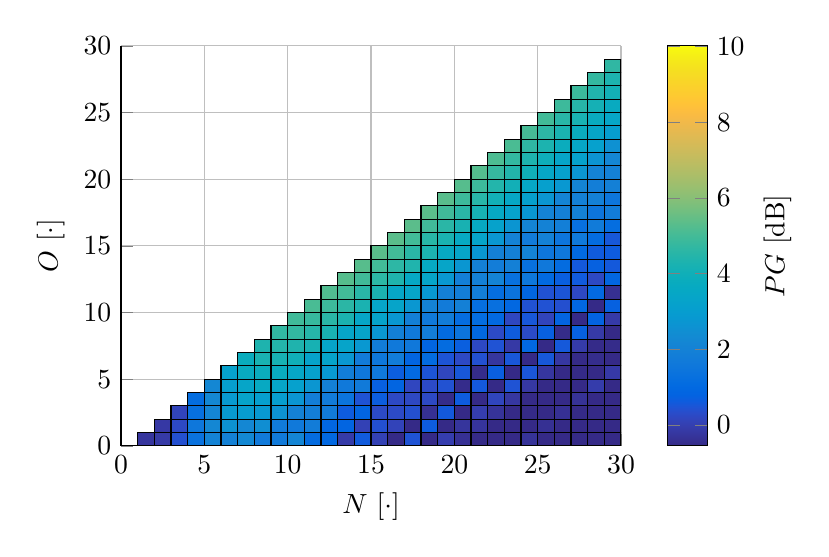
\begin{tikzpicture}


\begin{axis}[%
width=2.5in,
height=2in,
scale only axis,
point meta min=-0.551769511455843,
point meta max=10.0207598959184,
unbounded coords=jump,
xmin=0,
xmax=3000,
xlabel={$N$ [$\cdot$]},
xmajorgrids,
ymin=0,
ymax=3000,
ytick={0,500,...,3000},
yticklabels={0,5,...,30},
xtick={0,500,...,3000},
xticklabels={0,5,...,30},
ylabel={$O$ [$\cdot$]},
ymajorgrids,
axis background/.style={fill=white},
axis x line*=bottom,
axis y line*=left,
colormap={mymap}{[1pt] rgb(0pt)=(0.2081,0.1663,0.5292); rgb(1pt)=(0.211624,0.189781,0.577676); rgb(2pt)=(0.212252,0.213771,0.626971); rgb(3pt)=(0.2081,0.2386,0.677086); rgb(4pt)=(0.195905,0.264457,0.7279); rgb(5pt)=(0.170729,0.291938,0.779248); rgb(6pt)=(0.125271,0.324243,0.830271); rgb(7pt)=(0.0591333,0.359833,0.868333); rgb(8pt)=(0.0116952,0.38751,0.881957); rgb(9pt)=(0.00595714,0.408614,0.882843); rgb(10pt)=(0.0165143,0.4266,0.878633); rgb(11pt)=(0.0328524,0.443043,0.871957); rgb(12pt)=(0.0498143,0.458571,0.864057); rgb(13pt)=(0.0629333,0.47369,0.855438); rgb(14pt)=(0.0722667,0.488667,0.8467); rgb(15pt)=(0.0779429,0.503986,0.838371); rgb(16pt)=(0.0793476,0.520024,0.831181); rgb(17pt)=(0.0749429,0.537543,0.826271); rgb(18pt)=(0.0640571,0.556986,0.823957); rgb(19pt)=(0.0487714,0.577224,0.822829); rgb(20pt)=(0.0343429,0.596581,0.819852); rgb(21pt)=(0.0265,0.6137,0.8135); rgb(22pt)=(0.0238905,0.628662,0.803762); rgb(23pt)=(0.0230905,0.641786,0.791267); rgb(24pt)=(0.0227714,0.653486,0.776757); rgb(25pt)=(0.0266619,0.664195,0.760719); rgb(26pt)=(0.0383714,0.674271,0.743552); rgb(27pt)=(0.0589714,0.683757,0.725386); rgb(28pt)=(0.0843,0.692833,0.706167); rgb(29pt)=(0.113295,0.7015,0.685857); rgb(30pt)=(0.145271,0.709757,0.664629); rgb(31pt)=(0.180133,0.717657,0.642433); rgb(32pt)=(0.217829,0.725043,0.619262); rgb(33pt)=(0.258643,0.731714,0.595429); rgb(34pt)=(0.302171,0.737605,0.571186); rgb(35pt)=(0.348167,0.742433,0.547267); rgb(36pt)=(0.395257,0.7459,0.524443); rgb(37pt)=(0.44201,0.748081,0.503314); rgb(38pt)=(0.487124,0.749062,0.483976); rgb(39pt)=(0.530029,0.749114,0.466114); rgb(40pt)=(0.570857,0.748519,0.44939); rgb(41pt)=(0.609852,0.747314,0.433686); rgb(42pt)=(0.6473,0.7456,0.4188); rgb(43pt)=(0.683419,0.743476,0.404433); rgb(44pt)=(0.71841,0.741133,0.390476); rgb(45pt)=(0.752486,0.7384,0.376814); rgb(46pt)=(0.785843,0.735567,0.363271); rgb(47pt)=(0.818505,0.732733,0.34979); rgb(48pt)=(0.850657,0.7299,0.336029); rgb(49pt)=(0.882433,0.727433,0.3217); rgb(50pt)=(0.913933,0.725786,0.306276); rgb(51pt)=(0.944957,0.726114,0.288643); rgb(52pt)=(0.973895,0.731395,0.266648); rgb(53pt)=(0.993771,0.745457,0.240348); rgb(54pt)=(0.999043,0.765314,0.216414); rgb(55pt)=(0.995533,0.786057,0.196652); rgb(56pt)=(0.988,0.8066,0.179367); rgb(57pt)=(0.978857,0.827143,0.163314); rgb(58pt)=(0.9697,0.848138,0.147452); rgb(59pt)=(0.962586,0.870514,0.1309); rgb(60pt)=(0.958871,0.8949,0.113243); rgb(61pt)=(0.959824,0.921833,0.0948381); rgb(62pt)=(0.9661,0.951443,0.0755333); rgb(63pt)=(0.9763,0.9831,0.0538)},
colorbar,
colorbar style={ylabel={$PG$ [dB]}}
]

\addplot[%
surf,
shader=flat corner,draw=black,colormap={mymap}{[1pt] rgb(0pt)=(0.2081,0.1663,0.5292); rgb(1pt)=(0.211624,0.189781,0.577676); rgb(2pt)=(0.212252,0.213771,0.626971); rgb(3pt)=(0.2081,0.2386,0.677086); rgb(4pt)=(0.195905,0.264457,0.7279); rgb(5pt)=(0.170729,0.291938,0.779248); rgb(6pt)=(0.125271,0.324243,0.830271); rgb(7pt)=(0.0591333,0.359833,0.868333); rgb(8pt)=(0.0116952,0.38751,0.881957); rgb(9pt)=(0.00595714,0.408614,0.882843); rgb(10pt)=(0.0165143,0.4266,0.878633); rgb(11pt)=(0.0328524,0.443043,0.871957); rgb(12pt)=(0.0498143,0.458571,0.864057); rgb(13pt)=(0.0629333,0.47369,0.855438); rgb(14pt)=(0.0722667,0.488667,0.8467); rgb(15pt)=(0.0779429,0.503986,0.838371); rgb(16pt)=(0.0793476,0.520024,0.831181); rgb(17pt)=(0.0749429,0.537543,0.826271); rgb(18pt)=(0.0640571,0.556986,0.823957); rgb(19pt)=(0.0487714,0.577224,0.822829); rgb(20pt)=(0.0343429,0.596581,0.819852); rgb(21pt)=(0.0265,0.6137,0.8135); rgb(22pt)=(0.0238905,0.628662,0.803762); rgb(23pt)=(0.0230905,0.641786,0.791267); rgb(24pt)=(0.0227714,0.653486,0.776757); rgb(25pt)=(0.0266619,0.664195,0.760719); rgb(26pt)=(0.0383714,0.674271,0.743552); rgb(27pt)=(0.0589714,0.683757,0.725386); rgb(28pt)=(0.0843,0.692833,0.706167); rgb(29pt)=(0.113295,0.7015,0.685857); rgb(30pt)=(0.145271,0.709757,0.664629); rgb(31pt)=(0.180133,0.717657,0.642433); rgb(32pt)=(0.217829,0.725043,0.619262); rgb(33pt)=(0.258643,0.731714,0.595429); rgb(34pt)=(0.302171,0.737605,0.571186); rgb(35pt)=(0.348167,0.742433,0.547267); rgb(36pt)=(0.395257,0.7459,0.524443); rgb(37pt)=(0.44201,0.748081,0.503314); rgb(38pt)=(0.487124,0.749062,0.483976); rgb(39pt)=(0.530029,0.749114,0.466114); rgb(40pt)=(0.570857,0.748519,0.44939); rgb(41pt)=(0.609852,0.747314,0.433686); rgb(42pt)=(0.6473,0.7456,0.4188); rgb(43pt)=(0.683419,0.743476,0.404433); rgb(44pt)=(0.71841,0.741133,0.390476); rgb(45pt)=(0.752486,0.7384,0.376814); rgb(46pt)=(0.785843,0.735567,0.363271); rgb(47pt)=(0.818505,0.732733,0.34979); rgb(48pt)=(0.850657,0.7299,0.336029); rgb(49pt)=(0.882433,0.727433,0.3217); rgb(50pt)=(0.913933,0.725786,0.306276); rgb(51pt)=(0.944957,0.726114,0.288643); rgb(52pt)=(0.973895,0.731395,0.266648); rgb(53pt)=(0.993771,0.745457,0.240348); rgb(54pt)=(0.999043,0.765314,0.216414); rgb(55pt)=(0.995533,0.786057,0.196652); rgb(56pt)=(0.988,0.8066,0.179367); rgb(57pt)=(0.978857,0.827143,0.163314); rgb(58pt)=(0.9697,0.848138,0.147452); rgb(59pt)=(0.962586,0.870514,0.1309); rgb(60pt)=(0.958871,0.8949,0.113243); rgb(61pt)=(0.959824,0.921833,0.0948381); rgb(62pt)=(0.9661,0.951443,0.0755333); rgb(63pt)=(0.9763,0.9831,0.0538)},mesh/rows=30]
table[row sep=crcr, point meta=\thisrow{c}] {%
	%
	x	y	c\\
	100	0	-0.249851110691807\\
	100	100	nan\\
	100	200	nan\\
	100	300	nan\\
	100	400	nan\\
	100	500	nan\\
	100	600	nan\\
	100	700	nan\\
	100	800	nan\\
	100	900	nan\\
	100	1000	nan\\
	100	1100	nan\\
	100	1200	nan\\
	100	1300	nan\\
	100	1400	nan\\
	100	1500	nan\\
	100	1600	nan\\
	100	1700	nan\\
	100	1800	nan\\
	100	1900	nan\\
	100	2000	nan\\
	100	2100	nan\\
	100	2200	nan\\
	100	2300	nan\\
	100	2400	nan\\
	100	2500	nan\\
	100	2600	nan\\
	100	2700	nan\\
	100	2800	nan\\
	100	2900	nan\\
	200	0	-0.134212977797894\\
	200	100	-0.167103642187056\\
	200	200	nan\\
	200	300	nan\\
	200	400	nan\\
	200	500	nan\\
	200	600	nan\\
	200	700	nan\\
	200	800	nan\\
	200	900	nan\\
	200	1000	nan\\
	200	1100	nan\\
	200	1200	nan\\
	200	1300	nan\\
	200	1400	nan\\
	200	1500	nan\\
	200	1600	nan\\
	200	1700	nan\\
	200	1800	nan\\
	200	1900	nan\\
	200	2000	nan\\
	200	2100	nan\\
	200	2200	nan\\
	200	2300	nan\\
	200	2400	nan\\
	200	2500	nan\\
	200	2600	nan\\
	200	2700	nan\\
	200	2800	nan\\
	200	2900	nan\\
	300	0	0.40073258158409\\
	300	100	0.251927782024709\\
	300	200	0.142801564300892\\
	300	300	nan\\
	300	400	nan\\
	300	500	nan\\
	300	600	nan\\
	300	700	nan\\
	300	800	nan\\
	300	900	nan\\
	300	1000	nan\\
	300	1100	nan\\
	300	1200	nan\\
	300	1300	nan\\
	300	1400	nan\\
	300	1500	nan\\
	300	1600	nan\\
	300	1700	nan\\
	300	1800	nan\\
	300	1900	nan\\
	300	2000	nan\\
	300	2100	nan\\
	300	2200	nan\\
	300	2300	nan\\
	300	2400	nan\\
	300	2500	nan\\
	300	2600	nan\\
	300	2700	nan\\
	300	2800	nan\\
	300	2900	nan\\
	400	0	1.35498518276026\\
	400	100	1.54062929586375\\
	400	200	1.25091430573651\\
	400	300	1.13011541776478\\
	400	400	nan\\
	400	500	nan\\
	400	600	nan\\
	400	700	nan\\
	400	800	nan\\
	400	900	nan\\
	400	1000	nan\\
	400	1100	nan\\
	400	1200	nan\\
	400	1300	nan\\
	400	1400	nan\\
	400	1500	nan\\
	400	1600	nan\\
	400	1700	nan\\
	400	1800	nan\\
	400	1900	nan\\
	400	2000	nan\\
	400	2100	nan\\
	400	2200	nan\\
	400	2300	nan\\
	400	2400	nan\\
	400	2500	nan\\
	400	2600	nan\\
	400	2700	nan\\
	400	2800	nan\\
	400	2900	nan\\
	500	0	2.07613030072784\\
	500	100	2.23484268450241\\
	500	200	2.16667780407076\\
	500	300	2.22280459708376\\
	500	400	2.22773910206715\\
	500	500	nan\\
	500	600	nan\\
	500	700	nan\\
	500	800	nan\\
	500	900	nan\\
	500	1000	nan\\
	500	1100	nan\\
	500	1200	nan\\
	500	1300	nan\\
	500	1400	nan\\
	500	1500	nan\\
	500	1600	nan\\
	500	1700	nan\\
	500	1800	nan\\
	500	1900	nan\\
	500	2000	nan\\
	500	2100	nan\\
	500	2200	nan\\
	500	2300	nan\\
	500	2400	nan\\
	500	2500	nan\\
	500	2600	nan\\
	500	2700	nan\\
	500	2800	nan\\
	500	2900	nan\\
	600	0	2.0053564589082\\
	600	100	2.61259722918176\\
	600	200	2.8832092344045\\
	600	300	2.86284941749047\\
	600	400	3.10314445957564\\
	600	500	3.19779941497919\\
	600	600	nan\\
	600	700	nan\\
	600	800	nan\\
	600	900	nan\\
	600	1000	nan\\
	600	1100	nan\\
	600	1200	nan\\
	600	1300	nan\\
	600	1400	nan\\
	600	1500	nan\\
	600	1600	nan\\
	600	1700	nan\\
	600	1800	nan\\
	600	1900	nan\\
	600	2000	nan\\
	600	2100	nan\\
	600	2200	nan\\
	600	2300	nan\\
	600	2400	nan\\
	600	2500	nan\\
	600	2600	nan\\
	600	2700	nan\\
	600	2800	nan\\
	600	2900	nan\\
	700	0	2.2744146608244\\
	700	100	2.21229720700257\\
	700	200	2.93838458205897\\
	700	300	3.29709652218325\\
	700	400	3.37210041995159\\
	700	500	3.73517577501174\\
	700	600	3.8204270648783\\
	700	700	nan\\
	700	800	nan\\
	700	900	nan\\
	700	1000	nan\\
	700	1100	nan\\
	700	1200	nan\\
	700	1300	nan\\
	700	1400	nan\\
	700	1500	nan\\
	700	1600	nan\\
	700	1700	nan\\
	700	1800	nan\\
	700	1900	nan\\
	700	2000	nan\\
	700	2100	nan\\
	700	2200	nan\\
	700	2300	nan\\
	700	2400	nan\\
	700	2500	nan\\
	700	2600	nan\\
	700	2700	nan\\
	700	2800	nan\\
	700	2900	nan\\
	800	0	1.6764398517674\\
	800	100	2.47790908751089\\
	800	200	2.84811066063823\\
	800	300	3.0687707331656\\
	800	400	3.63876502838183\\
	800	500	3.84993979572264\\
	800	600	4.22707612972411\\
	800	700	4.34417470624987\\
	800	800	nan\\
	800	900	nan\\
	800	1000	nan\\
	800	1100	nan\\
	800	1200	nan\\
	800	1300	nan\\
	800	1400	nan\\
	800	1500	nan\\
	800	1600	nan\\
	800	1700	nan\\
	800	1800	nan\\
	800	1900	nan\\
	800	2000	nan\\
	800	2100	nan\\
	800	2200	nan\\
	800	2300	nan\\
	800	2400	nan\\
	800	2500	nan\\
	800	2600	nan\\
	800	2700	nan\\
	800	2800	nan\\
	800	2900	nan\\
	900	0	1.6957478568352\\
	900	100	1.7319915851467\\
	900	200	2.60512775573002\\
	900	300	2.98481824622671\\
	900	400	3.37091511369957\\
	900	500	3.74946849304965\\
	900	600	4.17472244368776\\
	900	700	4.46545647083027\\
	900	800	4.70107297446204\\
	900	900	nan\\
	900	1000	nan\\
	900	1100	nan\\
	900	1200	nan\\
	900	1300	nan\\
	900	1400	nan\\
	900	1500	nan\\
	900	1600	nan\\
	900	1700	nan\\
	900	1800	nan\\
	900	1900	nan\\
	900	2000	nan\\
	900	2100	nan\\
	900	2200	nan\\
	900	2300	nan\\
	900	2400	nan\\
	900	2500	nan\\
	900	2600	nan\\
	900	2700	nan\\
	900	2800	nan\\
	900	2900	nan\\
	1000	0	2.14279356476327\\
	1000	100	1.65662756562456\\
	1000	200	1.9975093051342\\
	1000	300	2.68811548919998\\
	1000	400	3.15564116436878\\
	1000	500	3.43923191192347\\
	1000	600	4.00698906883707\\
	1000	700	4.36135318968568\\
	1000	800	4.71880877909074\\
	1000	900	4.9493889064919\\
	1000	1000	nan\\
	1000	1100	nan\\
	1000	1200	nan\\
	1000	1300	nan\\
	1000	1400	nan\\
	1000	1500	nan\\
	1000	1600	nan\\
	1000	1700	nan\\
	1000	1800	nan\\
	1000	1900	nan\\
	1000	2000	nan\\
	1000	2100	nan\\
	1000	2200	nan\\
	1000	2300	nan\\
	1000	2400	nan\\
	1000	2500	nan\\
	1000	2600	nan\\
	1000	2700	nan\\
	1000	2800	nan\\
	1000	2900	nan\\
	1100	0	1.08628380389681\\
	1100	100	1.78373115008797\\
	1100	200	1.83869495569938\\
	1100	300	1.84921642836682\\
	1100	400	2.72090762354963\\
	1100	500	3.19932951902192\\
	1100	600	3.28763346728818\\
	1100	700	4.1733005127402\\
	1100	800	4.49383265009054\\
	1100	900	4.81677388898654\\
	1100	1000	5.09223132392375\\
	1100	1100	nan\\
	1100	1200	nan\\
	1100	1300	nan\\
	1100	1400	nan\\
	1100	1500	nan\\
	1100	1600	nan\\
	1100	1700	nan\\
	1100	1800	nan\\
	1100	1900	nan\\
	1100	2000	nan\\
	1100	2100	nan\\
	1100	2200	nan\\
	1100	2300	nan\\
	1100	2400	nan\\
	1100	2500	nan\\
	1100	2600	nan\\
	1100	2700	nan\\
	1100	2800	nan\\
	1100	2900	nan\\
	1200	0	0.96228292179036\\
	1200	100	0.874714526881095\\
	1200	200	1.74822965859813\\
	1200	300	1.74613873946482\\
	1200	400	1.96406088862939\\
	1200	500	2.83528036765025\\
	1200	600	3.27582233051984\\
	1200	700	3.34225172739605\\
	1200	800	4.2270814155954\\
	1200	900	4.5852271687131\\
	1200	1000	4.90782372375419\\
	1200	1100	5.19666553372495\\
	1200	1200	nan\\
	1200	1300	nan\\
	1200	1400	nan\\
	1200	1500	nan\\
	1200	1600	nan\\
	1200	1700	nan\\
	1200	1800	nan\\
	1200	1900	nan\\
	1200	2000	nan\\
	1200	2100	nan\\
	1200	2200	nan\\
	1200	2300	nan\\
	1200	2400	nan\\
	1200	2500	nan\\
	1200	2600	nan\\
	1200	2700	nan\\
	1200	2800	nan\\
	1200	2900	nan\\
	1300	0	-0.107030717223719\\
	1300	100	0.850232560605215\\
	1300	200	0.637949811893221\\
	1300	300	1.40384792467279\\
	1300	400	1.64958254277473\\
	1300	500	1.79741249348277\\
	1300	600	2.75608764238935\\
	1300	700	3.32534859240284\\
	1300	800	3.40167471419125\\
	1300	900	4.26932143570372\\
	1300	1000	4.60365364811444\\
	1300	1100	4.98195949948451\\
	1300	1200	5.28042149364273\\
	1300	1300	nan\\
	1300	1400	nan\\
	1300	1500	nan\\
	1300	1600	nan\\
	1300	1700	nan\\
	1300	1800	nan\\
	1300	1900	nan\\
	1300	2000	nan\\
	1300	2100	nan\\
	1300	2200	nan\\
	1300	2300	nan\\
	1300	2400	nan\\
	1300	2500	nan\\
	1300	2600	nan\\
	1300	2700	nan\\
	1300	2800	nan\\
	1300	2900	nan\\
	1400	0	0.601907313869925\\
	1400	100	0.0657729838043244\\
	1400	200	0.862145199127073\\
	1400	300	0.460707580490794\\
	1400	400	1.68525830954437\\
	1400	500	1.55802793388997\\
	1400	600	1.74594940231651\\
	1400	700	2.81551743753557\\
	1400	800	3.32371598632194\\
	1400	900	3.42520085860678\\
	1400	1000	4.25956377468848\\
	1400	1100	4.56477323219294\\
	1400	1200	4.97384046578701\\
	1400	1300	5.29633096641679\\
	1400	1400	nan\\
	1400	1500	nan\\
	1400	1600	nan\\
	1400	1700	nan\\
	1400	1800	nan\\
	1400	1900	nan\\
	1400	2000	nan\\
	1400	2100	nan\\
	1400	2200	nan\\
	1400	2300	nan\\
	1400	2400	nan\\
	1400	2500	nan\\
	1400	2600	nan\\
	1400	2700	nan\\
	1400	2800	nan\\
	1400	2900	nan\\
	1500	0	0.0479688920623348\\
	1500	100	0.409815317960011\\
	1500	200	0.265969244574455\\
	1500	300	0.66329040490881\\
	1500	400	0.725248934820509\\
	1500	500	1.62075499462296\\
	1500	600	1.53068266641447\\
	1500	700	1.78380983455356\\
	1500	800	2.75223306087479\\
	1500	900	3.29361894997763\\
	1500	1000	3.36423431504327\\
	1500	1100	4.28085176540069\\
	1500	1200	4.61221553749839\\
	1500	1300	4.99326970538795\\
	1500	1400	5.32976716671813\\
	1500	1500	nan\\
	1500	1600	nan\\
	1500	1700	nan\\
	1500	1800	nan\\
	1500	1900	nan\\
	1500	2000	nan\\
	1500	2100	nan\\
	1500	2200	nan\\
	1500	2300	nan\\
	1500	2400	nan\\
	1500	2500	nan\\
	1500	2600	nan\\
	1500	2700	nan\\
	1500	2800	nan\\
	1500	2900	nan\\
	1600	0	-0.605169389430681\\
	1600	100	0.117420548822926\\
	1600	200	0.284797641762555\\
	1600	300	0.253253520189372\\
	1600	400	0.870129979674615\\
	1600	500	0.671127168444688\\
	1600	600	1.74986538278574\\
	1600	700	1.64439306142093\\
	1600	800	1.91148110154675\\
	1600	900	2.77573952375898\\
	1600	1000	3.32540102344824\\
	1600	1100	3.44971766694812\\
	1600	1200	4.36003073667673\\
	1600	1300	4.62738934446695\\
	1600	1400	4.98723836519226\\
	1600	1500	5.34050250023747\\
	1600	1600	nan\\
	1600	1700	nan\\
	1600	1800	nan\\
	1600	1900	nan\\
	1600	2000	nan\\
	1600	2100	nan\\
	1600	2200	nan\\
	1600	2300	nan\\
	1600	2400	nan\\
	1600	2500	nan\\
	1600	2600	nan\\
	1600	2700	nan\\
	1600	2800	nan\\
	1600	2900	nan\\
	1700	0	0.459481577183121\\
	1700	100	-0.828238464808588\\
	1700	200	0.392172946743951\\
	1700	300	0.226384351456075\\
	1700	400	0.183454984733797\\
	1700	500	1.03300677343369\\
	1700	600	0.866722268193889\\
	1700	700	1.60939528933199\\
	1700	800	1.64458351852261\\
	1700	900	1.91984952325872\\
	1700	1000	2.75640854387435\\
	1700	1100	3.37358423554233\\
	1700	1200	3.57831957034059\\
	1700	1300	4.38037462195002\\
	1700	1400	4.57895857617312\\
	1700	1500	4.99333526811925\\
	1700	1600	5.35096269740123\\
	1700	1700	nan\\
	1700	1800	nan\\
	1700	1900	nan\\
	1700	2000	nan\\
	1700	2100	nan\\
	1700	2200	nan\\
	1700	2300	nan\\
	1700	2400	nan\\
	1700	2500	nan\\
	1700	2600	nan\\
	1700	2700	nan\\
	1700	2800	nan\\
	1700	2900	nan\\
	1800	0	-1.41853543923144\\
	1800	100	0.632649966343857\\
	1800	200	-0.384497042533314\\
	1800	300	0.255556860908392\\
	1800	400	0.286777052802089\\
	1800	500	0.482107568083193\\
	1800	600	1.07739734854062\\
	1800	700	0.851941681167397\\
	1800	800	1.82437185471004\\
	1800	900	1.65998697525295\\
	1800	1000	2.01342546713771\\
	1800	1100	2.84347279090459\\
	1800	1200	3.39849928401779\\
	1800	1300	3.59204978113913\\
	1800	1400	4.2917812700128\\
	1800	1500	4.54262260148609\\
	1800	1600	4.9656993136051\\
	1800	1700	5.33339229740171\\
	1800	1800	nan\\
	1800	1900	nan\\
	1800	2000	nan\\
	1800	2100	nan\\
	1800	2200	nan\\
	1800	2300	nan\\
	1800	2400	nan\\
	1800	2500	nan\\
	1800	2600	nan\\
	1800	2700	nan\\
	1800	2800	nan\\
	1800	2900	nan\\
	1900	0	-0.0337222813430315\\
	1900	100	-1.17881791521385\\
	1900	200	0.579738688002559\\
	1900	300	-0.504820413080548\\
	1900	400	0.43222545991656\\
	1900	500	0.172356634139464\\
	1900	600	0.486159910021189\\
	1900	700	1.08979803776635\\
	1900	800	1.06421189967321\\
	1900	900	1.76198646065506\\
	1900	1000	1.73893709942167\\
	1900	1100	1.94136948935232\\
	1900	1200	2.79511100023429\\
	1900	1300	3.40973957807585\\
	1900	1400	3.5985713113068\\
	1900	1500	4.25686359222365\\
	1900	1600	4.58134558875467\\
	1900	1700	4.95173298101252\\
	1900	1800	5.32121533683218\\
	1900	1900	nan\\
	1900	2000	nan\\
	1900	2100	nan\\
	1900	2200	nan\\
	1900	2300	nan\\
	1900	2400	nan\\
	1900	2500	nan\\
	1900	2600	nan\\
	1900	2700	nan\\
	1900	2800	nan\\
	1900	2900	nan\\
	2000	0	-0.38106458141862\\
	2000	100	-0.265003051545396\\
	2000	200	-1.23043392090561\\
	2000	300	0.636229173175987\\
	2000	400	-0.501393709183734\\
	2000	500	0.531105328460703\\
	2000	600	0.24654842554858\\
	2000	700	0.693751402870032\\
	2000	800	1.42643544661484\\
	2000	900	1.14002253653198\\
	2000	1000	1.9301916384988\\
	2000	1100	1.86037182253522\\
	2000	1200	1.89839206221938\\
	2000	1300	2.74843083934798\\
	2000	1400	3.37740852093157\\
	2000	1500	3.61406316805146\\
	2000	1600	4.20147952106818\\
	2000	1700	4.57501484363941\\
	2000	1800	4.91198130207837\\
	2000	1900	5.28767930948696\\
	2000	2000	nan\\
	2000	2100	nan\\
	2000	2200	nan\\
	2000	2300	nan\\
	2000	2400	nan\\
	2000	2500	nan\\
	2000	2600	nan\\
	2000	2700	nan\\
	2000	2800	nan\\
	2000	2900	nan\\
	2100	0	-2.54778888937748\\
	2100	100	-0.271665428891405\\
	2100	200	-0.0344816011139337\\
	2100	300	-0.92958440986473\\
	2100	400	0.578781786901553\\
	2100	500	-0.513825115608355\\
	2100	600	0.403549939556598\\
	2100	700	0.239133146523492\\
	2100	800	0.966867134182151\\
	2100	900	1.12439624993082\\
	2100	1000	1.21103058671727\\
	2100	1100	1.86790865947201\\
	2100	1200	1.93748456788468\\
	2100	1300	1.95877615912615\\
	2100	1400	2.77135113760514\\
	2100	1500	3.32533208850803\\
	2100	1600	3.62227458300587\\
	2100	1700	4.17113018391774\\
	2100	1800	4.53263736579035\\
	2100	1900	4.90200230486675\\
	2100	2000	5.25855080771329\\
	2100	2100	nan\\
	2100	2200	nan\\
	2100	2300	nan\\
	2100	2400	nan\\
	2100	2500	nan\\
	2100	2600	nan\\
	2100	2700	nan\\
	2100	2800	nan\\
	2100	2900	nan\\
	2200	0	-1.12219195506028\\
	2200	100	-1.31336747123425\\
	2200	200	-0.307205721342442\\
	2200	300	0.164262079814397\\
	2200	400	-1.21926646482995\\
	2200	500	0.69925026606895\\
	2200	600	-0.242343779721015\\
	2200	700	0.45336143020348\\
	2200	800	0.280137620132106\\
	2200	900	0.988124313583317\\
	2200	1000	1.26933662850539\\
	2200	1100	1.15533249489531\\
	2200	1200	2.06869578190726\\
	2200	1300	1.81246571931594\\
	2200	1400	1.95583313379746\\
	2200	1500	2.75579201352061\\
	2200	1600	3.23471519440769\\
	2200	1700	3.57001596339988\\
	2200	1800	4.06259292981595\\
	2200	1900	4.44509639802635\\
	2200	2000	4.78374621382732\\
	2200	2100	5.15758911026763\\
	2200	2200	nan\\
	2200	2300	nan\\
	2200	2400	nan\\
	2200	2500	nan\\
	2200	2600	nan\\
	2200	2700	nan\\
	2200	2800	nan\\
	2200	2900	nan\\
	2300	0	-1.47710144706725\\
	2300	100	-0.906455427488799\\
	2300	200	-1.98037240025395\\
	2300	300	-0.199957035643524\\
	2300	400	0.460748492052261\\
	2300	500	-0.991910728959527\\
	2300	600	0.525971155862777\\
	2300	700	-0.149701288761598\\
	2300	800	0.621750421643586\\
	2300	900	0.198409186972561\\
	2300	1000	0.945243542866472\\
	2300	1100	1.3863317144853\\
	2300	1200	1.28924677871813\\
	2300	1300	1.95854307882864\\
	2300	1400	1.95384530023978\\
	2300	1500	2.0261934442549\\
	2300	1600	2.7106344140713\\
	2300	1700	3.22197061661371\\
	2300	1800	3.52766026642127\\
	2300	1900	4.05537018397665\\
	2300	2000	4.41989791085985\\
	2300	2100	4.739244959608\\
	2300	2200	5.11505997170104\\
	2300	2300	nan\\
	2300	2400	nan\\
	2300	2500	nan\\
	2300	2600	nan\\
	2300	2700	nan\\
	2300	2800	nan\\
	2300	2900	nan\\
	2400	0	-0.320797119372326\\
	2400	100	-2.08086383335104\\
	2400	200	-0.720605194761059\\
	2400	300	-1.01717368621161\\
	2400	400	-0.187558838767389\\
	2400	500	0.507570513499698\\
	2400	600	-1.92928601081134\\
	2400	700	0.944348973287413\\
	2400	800	0.288636669596869\\
	2400	900	0.532260889332141\\
	2400	1000	0.443648390100737\\
	2400	1100	0.904358845508782\\
	2400	1200	1.53668027505922\\
	2400	1300	1.29827288576412\\
	2400	1400	2.07715564674529\\
	2400	1500	1.74697118825321\\
	2400	1600	2.12834984811783\\
	2400	1700	2.77936543889467\\
	2400	1800	3.1446297870471\\
	2400	1900	3.48831005734869\\
	2400	2000	4.00374071424347\\
	2400	2100	4.33580058800992\\
	2400	2200	4.67537063296036\\
	2400	2300	5.04789691319579\\
	2400	2400	nan\\
	2400	2500	nan\\
	2400	2600	nan\\
	2400	2700	nan\\
	2400	2800	nan\\
	2400	2900	nan\\
	2500	0	-2.0104573809398\\
	2500	100	-0.392343598865612\\
	2500	200	-1.8368666517391\\
	2500	300	-0.82371070662834\\
	2500	400	-1.32502823584576\\
	2500	500	-0.226000841089313\\
	2500	600	0.548661883474864\\
	2500	700	-0.563414840915817\\
	2500	800	0.719706683295337\\
	2500	900	0.139929086569895\\
	2500	1000	0.444214679076209\\
	2500	1100	0.434720509652219\\
	2500	1200	1.00838245548818\\
	2500	1300	1.61526525372892\\
	2500	1400	1.50483170501125\\
	2500	1500	1.97109888154096\\
	2500	1600	2.03226934513893\\
	2500	1700	2.06130742061999\\
	2500	1800	2.72129277515449\\
	2500	1900	3.1496302758595\\
	2500	2000	3.45936002063925\\
	2500	2100	3.94489565230288\\
	2500	2200	4.30572923130044\\
	2500	2300	4.62826739760606\\
	2500	2400	4.97957558003119\\
	2500	2500	nan\\
	2500	2600	nan\\
	2500	2700	nan\\
	2500	2800	nan\\
	2500	2900	nan\\
	2600	0	-1.04276669806063\\
	2600	100	-2.09416387271156\\
	2600	200	-0.393434047566139\\
	2600	300	-1.99744602321698\\
	2600	400	-0.732752927466251\\
	2600	500	-0.845072590898031\\
	2600	600	-0.197190057403832\\
	2600	700	0.568345161186178\\
	2600	800	-0.517339941265535\\
	2600	900	0.829926415452995\\
	2600	1000	0.390234771212351\\
	2600	1100	0.491755441545595\\
	2600	1200	0.704096258663999\\
	2600	1300	1.09324483879672\\
	2600	1400	1.57802894545829\\
	2600	1500	1.46114303849973\\
	2600	1600	1.90240313383773\\
	2600	1700	1.96492976302582\\
	2600	1800	2.10546989577579\\
	2600	1900	2.80784168171935\\
	2600	2000	3.16732452004093\\
	2600	2100	3.38561363290859\\
	2600	2200	3.84271392956099\\
	2600	2300	4.2572252696732\\
	2600	2400	4.56536241495736\\
	2600	2500	4.91098340653298\\
	2600	2600	nan\\
	2600	2700	nan\\
	2600	2800	nan\\
	2600	2900	nan\\
	2700	0	-1.86457281182685\\
	2700	100	-0.827278808604148\\
	2700	200	-1.66139059361561\\
	2700	300	-0.345864976502062\\
	2700	400	-1.7419225510789\\
	2700	500	-0.593489781608872\\
	2700	600	-0.862654185873941\\
	2700	700	-0.107262572069259\\
	2700	800	0.737413488411968\\
	2700	900	-0.576925684154879\\
	2700	1000	0.924482174160993\\
	2700	1100	0.231285101969482\\
	2700	1200	0.60757641237186\\
	2700	1300	0.572762239400506\\
	2700	1400	1.01681359955306\\
	2700	1500	1.62677895329449\\
	2700	1600	1.27480511346536\\
	2700	1700	1.98789624096392\\
	2700	1800	1.93276526620462\\
	2700	1900	2.10738766910072\\
	2700	2000	2.70916458298157\\
	2700	2100	3.16967395615291\\
	2700	2200	3.46065291646132\\
	2700	2300	3.81032783422735\\
	2700	2400	4.22415848460165\\
	2700	2500	4.52183620559259\\
	2700	2600	4.86759622928776\\
	2700	2700	nan\\
	2700	2800	nan\\
	2700	2900	nan\\
	2800	0	-1.49739781076471\\
	2800	100	-2.67774493578824\\
	2800	200	-0.77412049215611\\
	2800	300	-1.72011869579828\\
	2800	400	-0.0701188596208511\\
	2800	500	-1.70094265456318\\
	2800	600	-0.487531798132342\\
	2800	700	-0.529257096051941\\
	2800	800	-0.131151559110154\\
	2800	900	0.78957451991771\\
	2800	1000	-0.865476909209226\\
	2800	1100	1.02302973697698\\
	2800	1200	0.243101070085026\\
	2800	1300	0.742951511605838\\
	2800	1400	0.610390012352961\\
	2800	1500	1.11184992188686\\
	2800	1600	1.70635439698124\\
	2800	1700	1.46194552969499\\
	2800	1800	1.92924805240906\\
	2800	1900	1.87847517716547\\
	2800	2000	2.07312611768239\\
	2800	2100	2.66697340455749\\
	2800	2200	3.15331447101904\\
	2800	2300	3.41140837248757\\
	2800	2400	3.76235867111117\\
	2800	2500	4.12843111933201\\
	2800	2600	4.4023277472934\\
	2800	2700	4.76460244668478\\
	2800	2800	nan\\
	2800	2900	nan\\
	2900	0	-1.44796049191922\\
	2900	100	-1.66126441754841\\
	2900	200	-1.64805097723939\\
	2900	300	-0.886269859067559\\
	2900	400	-1.83897503635551\\
	2900	500	-0.139927916994236\\
	2900	600	-1.19931399987204\\
	2900	700	-0.511718884088781\\
	2900	800	-0.858784361504311\\
	2900	900	-0.115034369534619\\
	2900	1000	0.746626598284007\\
	2900	1100	-0.400257131855673\\
	2900	1200	0.882957675355658\\
	2900	1300	0.575440859539888\\
	2900	1400	0.631827605653908\\
	2900	1500	0.545218588180702\\
	2900	1600	1.15662298898431\\
	2900	1700	1.75394101641656\\
	2900	1800	1.49528551706079\\
	2900	1900	1.9571726486198\\
	2900	2000	1.98737859631502\\
	2900	2100	2.18129198607386\\
	2900	2200	2.578667434529\\
	2900	2300	3.05978925137697\\
	2900	2400	3.44203078641863\\
	2900	2500	3.71252197556382\\
	2900	2600	4.0899622658663\\
	2900	2700	4.31939684132165\\
	2900	2800	4.68481624670495\\
	2900	2900	nan\\
	3000	0	-1.82535121336032\\
	3000	100	-1.52645895463458\\
	3000	200	-1.31895300730491\\
	3000	300	-1.40799683045683\\
	3000	400	-0.608341004711642\\
	3000	500	-1.49040055505408\\
	3000	600	-0.00822542843949026\\
	3000	700	-1.4811075478664\\
	3000	800	-0.447408269853539\\
	3000	900	-0.834756167944264\\
	3000	1000	-0.177702447283364\\
	3000	1100	0.81138170474657\\
	3000	1200	-0.19145895641342\\
	3000	1300	0.846154256563536\\
	3000	1400	0.435364626531824\\
	3000	1500	0.602638318388225\\
	3000	1600	0.624526481274859\\
	3000	1700	1.22635866276765\\
	3000	1800	1.71794544510154\\
	3000	1900	1.60268215825526\\
	3000	2000	1.98278562327647\\
	3000	2100	1.98408241916151\\
	3000	2200	2.18214168927242\\
	3000	2300	2.61007421484023\\
	3000	2400	3.01983476549906\\
	3000	2500	3.30889872378107\\
	3000	2600	3.66409137003239\\
	3000	2700	4.04006487090192\\
	3000	2800	4.29517382850778\\
	3000	2900	4.64867996838188\\
};
\end{axis}
\end{tikzpicture}%}
%		\end{column}
%	\end{columns}
%\end{frame}
%
%\begin{frame}{Simulation Results}{Optimal parameters P=10}		
%	\begin{columns}
%		\begin{column}{0.4\textwidth}
%			\begin{itemize}
%				\item Prediction order P = 10
%				\item Optimal parameters
%				\begin{itemize}
%					\item Framelength N = 1200
%					\item Overlap O = 1100
%				\end{itemize}
%				\item Prediction Gain PG = 10 dB
%			\end{itemize}
%		\end{column}
%		\begin{column}{0.6\textwidth} 
%			\resizebox{0.9\columnwidth}{!}{		
%				% This file was created by matlab2tikz.
%
%The latest updates can be retrieved from
%  http://www.mathworks.com/matlabcentral/fileexchange/22022-matlab2tikz-matlab2tikz
%where you can also make suggestions and rate matlab2tikz.
%
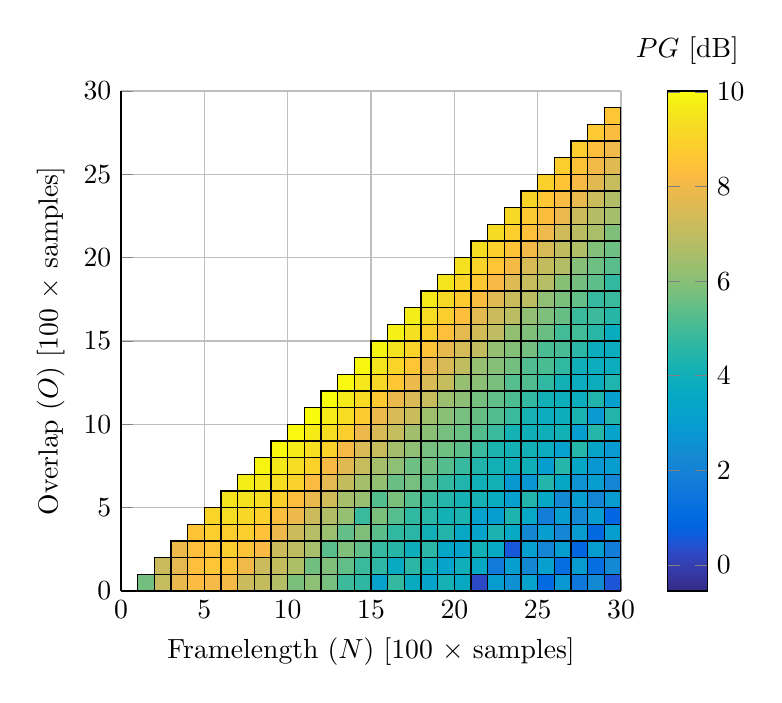
\begin{tikzpicture}


\begin{axis}[%
width=2.5in,
height=2.5in,
scale only axis,
point meta min=-0.551769511455843,
point meta max=10.0207598959184,
unbounded coords=jump,
xmin=0,
xmax=3000,
xlabel={Framelength ($N$) [100 $\times$ samples]},
xmajorgrids,
ymin=0,
ymax=3000,
ytick={0,500,...,3000},
yticklabels={0,5,...,30},
xtick={0,500,...,3000},
xticklabels={0,5,...,30},
ylabel={Overlap ($O$) [100 $\times$ samples]},
ymajorgrids,
axis background/.style={fill=white},
axis x line*=bottom,
axis y line*=left,
colormap={mymap}{[1pt] rgb(0pt)=(0.2081,0.1663,0.5292); rgb(1pt)=(0.211624,0.189781,0.577676); rgb(2pt)=(0.212252,0.213771,0.626971); rgb(3pt)=(0.2081,0.2386,0.677086); rgb(4pt)=(0.195905,0.264457,0.7279); rgb(5pt)=(0.170729,0.291938,0.779248); rgb(6pt)=(0.125271,0.324243,0.830271); rgb(7pt)=(0.0591333,0.359833,0.868333); rgb(8pt)=(0.0116952,0.38751,0.881957); rgb(9pt)=(0.00595714,0.408614,0.882843); rgb(10pt)=(0.0165143,0.4266,0.878633); rgb(11pt)=(0.0328524,0.443043,0.871957); rgb(12pt)=(0.0498143,0.458571,0.864057); rgb(13pt)=(0.0629333,0.47369,0.855438); rgb(14pt)=(0.0722667,0.488667,0.8467); rgb(15pt)=(0.0779429,0.503986,0.838371); rgb(16pt)=(0.0793476,0.520024,0.831181); rgb(17pt)=(0.0749429,0.537543,0.826271); rgb(18pt)=(0.0640571,0.556986,0.823957); rgb(19pt)=(0.0487714,0.577224,0.822829); rgb(20pt)=(0.0343429,0.596581,0.819852); rgb(21pt)=(0.0265,0.6137,0.8135); rgb(22pt)=(0.0238905,0.628662,0.803762); rgb(23pt)=(0.0230905,0.641786,0.791267); rgb(24pt)=(0.0227714,0.653486,0.776757); rgb(25pt)=(0.0266619,0.664195,0.760719); rgb(26pt)=(0.0383714,0.674271,0.743552); rgb(27pt)=(0.0589714,0.683757,0.725386); rgb(28pt)=(0.0843,0.692833,0.706167); rgb(29pt)=(0.113295,0.7015,0.685857); rgb(30pt)=(0.145271,0.709757,0.664629); rgb(31pt)=(0.180133,0.717657,0.642433); rgb(32pt)=(0.217829,0.725043,0.619262); rgb(33pt)=(0.258643,0.731714,0.595429); rgb(34pt)=(0.302171,0.737605,0.571186); rgb(35pt)=(0.348167,0.742433,0.547267); rgb(36pt)=(0.395257,0.7459,0.524443); rgb(37pt)=(0.44201,0.748081,0.503314); rgb(38pt)=(0.487124,0.749062,0.483976); rgb(39pt)=(0.530029,0.749114,0.466114); rgb(40pt)=(0.570857,0.748519,0.44939); rgb(41pt)=(0.609852,0.747314,0.433686); rgb(42pt)=(0.6473,0.7456,0.4188); rgb(43pt)=(0.683419,0.743476,0.404433); rgb(44pt)=(0.71841,0.741133,0.390476); rgb(45pt)=(0.752486,0.7384,0.376814); rgb(46pt)=(0.785843,0.735567,0.363271); rgb(47pt)=(0.818505,0.732733,0.34979); rgb(48pt)=(0.850657,0.7299,0.336029); rgb(49pt)=(0.882433,0.727433,0.3217); rgb(50pt)=(0.913933,0.725786,0.306276); rgb(51pt)=(0.944957,0.726114,0.288643); rgb(52pt)=(0.973895,0.731395,0.266648); rgb(53pt)=(0.993771,0.745457,0.240348); rgb(54pt)=(0.999043,0.765314,0.216414); rgb(55pt)=(0.995533,0.786057,0.196652); rgb(56pt)=(0.988,0.8066,0.179367); rgb(57pt)=(0.978857,0.827143,0.163314); rgb(58pt)=(0.9697,0.848138,0.147452); rgb(59pt)=(0.962586,0.870514,0.1309); rgb(60pt)=(0.958871,0.8949,0.113243); rgb(61pt)=(0.959824,0.921833,0.0948381); rgb(62pt)=(0.9661,0.951443,0.0755333); rgb(63pt)=(0.9763,0.9831,0.0538)},
colorbar,
colorbar style={title=$PG$ [dB]}
]%ylabel={PG}

\addplot[%
surf,
opacity = ceil(\pgfplotspointmetatransformed),
shader=flat corner,draw=black,colormap={mymap}{[1pt] rgb(0pt)=(0.2081,0.1663,0.5292); rgb(1pt)=(0.211624,0.189781,0.577676); rgb(2pt)=(0.212252,0.213771,0.626971); rgb(3pt)=(0.2081,0.2386,0.677086); rgb(4pt)=(0.195905,0.264457,0.7279); rgb(5pt)=(0.170729,0.291938,0.779248); rgb(6pt)=(0.125271,0.324243,0.830271); rgb(7pt)=(0.0591333,0.359833,0.868333); rgb(8pt)=(0.0116952,0.38751,0.881957); rgb(9pt)=(0.00595714,0.408614,0.882843); rgb(10pt)=(0.0165143,0.4266,0.878633); rgb(11pt)=(0.0328524,0.443043,0.871957); rgb(12pt)=(0.0498143,0.458571,0.864057); rgb(13pt)=(0.0629333,0.47369,0.855438); rgb(14pt)=(0.0722667,0.488667,0.8467); rgb(15pt)=(0.0779429,0.503986,0.838371); rgb(16pt)=(0.0793476,0.520024,0.831181); rgb(17pt)=(0.0749429,0.537543,0.826271); rgb(18pt)=(0.0640571,0.556986,0.823957); rgb(19pt)=(0.0487714,0.577224,0.822829); rgb(20pt)=(0.0343429,0.596581,0.819852); rgb(21pt)=(0.0265,0.6137,0.8135); rgb(22pt)=(0.0238905,0.628662,0.803762); rgb(23pt)=(0.0230905,0.641786,0.791267); rgb(24pt)=(0.0227714,0.653486,0.776757); rgb(25pt)=(0.0266619,0.664195,0.760719); rgb(26pt)=(0.0383714,0.674271,0.743552); rgb(27pt)=(0.0589714,0.683757,0.725386); rgb(28pt)=(0.0843,0.692833,0.706167); rgb(29pt)=(0.113295,0.7015,0.685857); rgb(30pt)=(0.145271,0.709757,0.664629); rgb(31pt)=(0.180133,0.717657,0.642433); rgb(32pt)=(0.217829,0.725043,0.619262); rgb(33pt)=(0.258643,0.731714,0.595429); rgb(34pt)=(0.302171,0.737605,0.571186); rgb(35pt)=(0.348167,0.742433,0.547267); rgb(36pt)=(0.395257,0.7459,0.524443); rgb(37pt)=(0.44201,0.748081,0.503314); rgb(38pt)=(0.487124,0.749062,0.483976); rgb(39pt)=(0.530029,0.749114,0.466114); rgb(40pt)=(0.570857,0.748519,0.44939); rgb(41pt)=(0.609852,0.747314,0.433686); rgb(42pt)=(0.6473,0.7456,0.4188); rgb(43pt)=(0.683419,0.743476,0.404433); rgb(44pt)=(0.71841,0.741133,0.390476); rgb(45pt)=(0.752486,0.7384,0.376814); rgb(46pt)=(0.785843,0.735567,0.363271); rgb(47pt)=(0.818505,0.732733,0.34979); rgb(48pt)=(0.850657,0.7299,0.336029); rgb(49pt)=(0.882433,0.727433,0.3217); rgb(50pt)=(0.913933,0.725786,0.306276); rgb(51pt)=(0.944957,0.726114,0.288643); rgb(52pt)=(0.973895,0.731395,0.266648); rgb(53pt)=(0.993771,0.745457,0.240348); rgb(54pt)=(0.999043,0.765314,0.216414); rgb(55pt)=(0.995533,0.786057,0.196652); rgb(56pt)=(0.988,0.8066,0.179367); rgb(57pt)=(0.978857,0.827143,0.163314); rgb(58pt)=(0.9697,0.848138,0.147452); rgb(59pt)=(0.962586,0.870514,0.1309); rgb(60pt)=(0.958871,0.8949,0.113243); rgb(61pt)=(0.959824,0.921833,0.0948381); rgb(62pt)=(0.9661,0.951443,0.0755333); rgb(63pt)=(0.9763,0.9831,0.0538)},mesh/rows=30]
table[row sep=crcr, point meta=\thisrow{c}] {%
%
x	y	c\\
100	0	5.6827458135075\\
100	100	nan\\
100	200	nan\\
100	300	nan\\
100	400	nan\\
100	500	nan\\
100	600	nan\\
100	700	nan\\
100	800	nan\\
100	900	nan\\
100	1000	nan\\
100	1100	nan\\
100	1200	nan\\
100	1300	nan\\
100	1400	nan\\
100	1500	nan\\
100	1600	nan\\
100	1700	nan\\
100	1800	nan\\
100	1900	nan\\
100	2000	nan\\
100	2100	nan\\
100	2200	nan\\
100	2300	nan\\
100	2400	nan\\
100	2500	nan\\
100	2600	nan\\
100	2700	nan\\
100	2800	nan\\
100	2900	nan\\
200	0	7.0790317182078\\
200	100	7.18389489543295\\
200	200	nan\\
200	300	nan\\
200	400	nan\\
200	500	nan\\
200	600	nan\\
200	700	nan\\
200	800	nan\\
200	900	nan\\
200	1000	nan\\
200	1100	nan\\
200	1200	nan\\
200	1300	nan\\
200	1400	nan\\
200	1500	nan\\
200	1600	nan\\
200	1700	nan\\
200	1800	nan\\
200	1900	nan\\
200	2000	nan\\
200	2100	nan\\
200	2200	nan\\
200	2300	nan\\
200	2400	nan\\
200	2500	nan\\
200	2600	nan\\
200	2700	nan\\
200	2800	nan\\
200	2900	nan\\
300	0	7.8278797182668\\
300	100	7.75061670667307\\
300	200	7.94964232573768\\
300	300	nan\\
300	400	nan\\
300	500	nan\\
300	600	nan\\
300	700	nan\\
300	800	nan\\
300	900	nan\\
300	1000	nan\\
300	1100	nan\\
300	1200	nan\\
300	1300	nan\\
300	1400	nan\\
300	1500	nan\\
300	1600	nan\\
300	1700	nan\\
300	1800	nan\\
300	1900	nan\\
300	2000	nan\\
300	2100	nan\\
300	2200	nan\\
300	2300	nan\\
300	2400	nan\\
300	2500	nan\\
300	2600	nan\\
300	2700	nan\\
300	2800	nan\\
300	2900	nan\\
400	0	8.25982045157361\\
400	100	8.37365829237133\\
400	200	8.38994845512447\\
400	300	8.53395155897113\\
400	400	nan\\
400	500	nan\\
400	600	nan\\
400	700	nan\\
400	800	nan\\
400	900	nan\\
400	1000	nan\\
400	1100	nan\\
400	1200	nan\\
400	1300	nan\\
400	1400	nan\\
400	1500	nan\\
400	1600	nan\\
400	1700	nan\\
400	1800	nan\\
400	1900	nan\\
400	2000	nan\\
400	2100	nan\\
400	2200	nan\\
400	2300	nan\\
400	2400	nan\\
400	2500	nan\\
400	2600	nan\\
400	2700	nan\\
400	2800	nan\\
400	2900	nan\\
500	0	8.09522110947221\\
500	100	8.58404936019439\\
500	200	8.52476852167647\\
500	300	8.85395289600773\\
500	400	9.03400135477561\\
500	500	nan\\
500	600	nan\\
500	700	nan\\
500	800	nan\\
500	900	nan\\
500	1000	nan\\
500	1100	nan\\
500	1200	nan\\
500	1300	nan\\
500	1400	nan\\
500	1500	nan\\
500	1600	nan\\
500	1700	nan\\
500	1800	nan\\
500	1900	nan\\
500	2000	nan\\
500	2100	nan\\
500	2200	nan\\
500	2300	nan\\
500	2400	nan\\
500	2500	nan\\
500	2600	nan\\
500	2700	nan\\
500	2800	nan\\
500	2900	nan\\
600	0	8.05650724153339\\
600	100	8.54693570913705\\
600	200	8.8377683265956\\
600	300	8.82559971223848\\
600	400	9.28658312212634\\
600	500	9.52161535433559\\
600	600	nan\\
600	700	nan\\
600	800	nan\\
600	900	nan\\
600	1000	nan\\
600	1100	nan\\
600	1200	nan\\
600	1300	nan\\
600	1400	nan\\
600	1500	nan\\
600	1600	nan\\
600	1700	nan\\
600	1800	nan\\
600	1900	nan\\
600	2000	nan\\
600	2100	nan\\
600	2200	nan\\
600	2300	nan\\
600	2400	nan\\
600	2500	nan\\
600	2600	nan\\
600	2700	nan\\
600	2800	nan\\
600	2900	nan\\
700	0	7.20736652003549\\
700	100	8.01860060821804\\
700	200	8.5092217869215\\
700	300	8.85498614721321\\
700	400	9.13100370114176\\
700	500	9.43150883603405\\
700	600	9.74782220562509\\
700	700	nan\\
700	800	nan\\
700	900	nan\\
700	1000	nan\\
700	1100	nan\\
700	1200	nan\\
700	1300	nan\\
700	1400	nan\\
700	1500	nan\\
700	1600	nan\\
700	1700	nan\\
700	1800	nan\\
700	1900	nan\\
700	2000	nan\\
700	2100	nan\\
700	2200	nan\\
700	2300	nan\\
700	2400	nan\\
700	2500	nan\\
700	2600	nan\\
700	2700	nan\\
700	2800	nan\\
700	2900	nan\\
800	0	7.06129617908756\\
800	100	7.21625389795336\\
800	200	8.17024678080842\\
800	300	8.4506398874489\\
800	400	8.92543148972206\\
800	500	9.31059383665309\\
800	600	9.57358732259701\\
800	700	9.88474425342921\\
800	800	nan\\
800	900	nan\\
800	1000	nan\\
800	1100	nan\\
800	1200	nan\\
800	1300	nan\\
800	1400	nan\\
800	1500	nan\\
800	1600	nan\\
800	1700	nan\\
800	1800	nan\\
800	1900	nan\\
800	2000	nan\\
800	2100	nan\\
800	2200	nan\\
800	2300	nan\\
800	2400	nan\\
800	2500	nan\\
800	2600	nan\\
800	2700	nan\\
800	2800	nan\\
800	2900	nan\\
900	0	6.7603240209297\\
900	100	7.07027516643772\\
900	200	7.21503157848168\\
900	300	7.91680228410601\\
900	400	8.33413384154289\\
900	500	8.91700110520262\\
900	600	9.33441266257382\\
900	700	9.61050000584357\\
900	800	9.96602273571317\\
900	900	nan\\
900	1000	nan\\
900	1100	nan\\
900	1200	nan\\
900	1300	nan\\
900	1400	nan\\
900	1500	nan\\
900	1600	nan\\
900	1700	nan\\
900	1800	nan\\
900	1900	nan\\
900	2000	nan\\
900	2100	nan\\
900	2200	nan\\
900	2300	nan\\
900	2400	nan\\
900	2500	nan\\
900	2600	nan\\
900	2700	nan\\
900	2800	nan\\
900	2900	nan\\
1000	0	5.79141266758575\\
1000	100	6.6583846543796\\
1000	200	6.96560213501504\\
1000	300	7.24068731658401\\
1000	400	7.9395591224285\\
1000	500	8.31867811054653\\
1000	600	8.9754932003346\\
1000	700	9.34845065231673\\
1000	800	9.67344129050852\\
1000	900	9.99470564606262\\
1000	1000	nan\\
1000	1100	nan\\
1000	1200	nan\\
1000	1300	nan\\
1000	1400	nan\\
1000	1500	nan\\
1000	1600	nan\\
1000	1700	nan\\
1000	1800	nan\\
1000	1900	nan\\
1000	2000	nan\\
1000	2100	nan\\
1000	2200	nan\\
1000	2300	nan\\
1000	2400	nan\\
1000	2500	nan\\
1000	2600	nan\\
1000	2700	nan\\
1000	2800	nan\\
1000	2900	nan\\
1100	0	6.08510006030311\\
1100	100	5.66131684642677\\
1100	200	6.52494101151453\\
1100	300	6.8154749961067\\
1100	400	7.2221683246724\\
1100	500	7.85272239575603\\
1100	600	8.25834444268623\\
1100	700	8.98246828788382\\
1100	800	9.38384280669374\\
1100	900	9.67888280713376\\
1100	1000	10.0207598959184\\
1100	1100	nan\\
1100	1200	nan\\
1100	1300	nan\\
1100	1400	nan\\
1100	1500	nan\\
1100	1600	nan\\
1100	1700	nan\\
1100	1800	nan\\
1100	1900	nan\\
1100	2000	nan\\
1100	2100	nan\\
1100	2200	nan\\
1100	2300	nan\\
1100	2400	nan\\
1100	2500	nan\\
1100	2600	nan\\
1100	2700	nan\\
1100	2800	nan\\
1100	2900	nan\\
1200	0	5.75236385929885\\
1200	100	5.8893978793085\\
1200	200	5.3233876826882\\
1200	300	6.30245671838949\\
1200	400	6.70416183583482\\
1200	500	7.29231639499116\\
1200	600	7.73083236703484\\
1200	700	8.13278866080154\\
1200	800	8.95016901139914\\
1200	900	9.3575654964583\\
1200	1000	9.69962351631871\\
1200	1100	10.018452727616\\
1200	1200	nan\\
1200	1300	nan\\
1200	1400	nan\\
1200	1500	nan\\
1200	1600	nan\\
1200	1700	nan\\
1200	1800	nan\\
1200	1900	nan\\
1200	2000	nan\\
1200	2100	nan\\
1200	2200	nan\\
1200	2300	nan\\
1200	2400	nan\\
1200	2500	nan\\
1200	2600	nan\\
1200	2700	nan\\
1200	2800	nan\\
1200	2900	nan\\
1300	0	4.8910628019805\\
1300	100	5.45072016874233\\
1300	200	5.86850066777867\\
1300	300	5.4597166268533\\
1300	400	6.21490882072339\\
1300	500	6.48849191466192\\
1300	600	7.05573401013256\\
1300	700	7.66870480877405\\
1300	800	8.12020714201073\\
1300	900	8.84241536316059\\
1300	1000	9.32521343768448\\
1300	1100	9.66682615033229\\
1300	1200	9.99393859933556\\
1300	1300	nan\\
1300	1400	nan\\
1300	1500	nan\\
1300	1600	nan\\
1300	1700	nan\\
1300	1800	nan\\
1300	1900	nan\\
1300	2000	nan\\
1300	2100	nan\\
1300	2200	nan\\
1300	2300	nan\\
1300	2400	nan\\
1300	2500	nan\\
1300	2600	nan\\
1300	2700	nan\\
1300	2800	nan\\
1300	2900	nan\\
1400	0	4.68328180207416\\
1400	100	4.87031890586883\\
1400	200	5.46124064783872\\
1400	300	5.87957713868692\\
1400	400	4.86401495955569\\
1400	500	6.26391766665361\\
1400	600	6.48566475687751\\
1400	700	7.13851035956643\\
1400	800	7.50027034876972\\
1400	900	7.94746340189027\\
1400	1000	8.77453134934714\\
1400	1100	9.23762319980819\\
1400	1200	9.58536439829166\\
1400	1300	9.93647418346277\\
1400	1400	nan\\
1400	1500	nan\\
1400	1600	nan\\
1400	1700	nan\\
1400	1800	nan\\
1400	1900	nan\\
1400	2000	nan\\
1400	2100	nan\\
1400	2200	nan\\
1400	2300	nan\\
1400	2400	nan\\
1400	2500	nan\\
1400	2600	nan\\
1400	2700	nan\\
1400	2800	nan\\
1400	2900	nan\\
1500	0	3.24765243794076\\
1500	100	4.65481232593174\\
1500	200	4.79830988957897\\
1500	300	5.35751567095906\\
1500	400	5.79287838471904\\
1500	500	5.25522140259071\\
1500	600	6.17072553135157\\
1500	700	6.48214041903959\\
1500	800	7.1345332299744\\
1500	900	7.48068047659614\\
1500	1000	7.89377405226484\\
1500	1100	8.70610504087698\\
1500	1200	9.16324372984275\\
1500	1300	9.52474035946379\\
1500	1400	9.86030813520319\\
1500	1500	nan\\
1500	1600	nan\\
1500	1700	nan\\
1500	1800	nan\\
1500	1900	nan\\
1500	2000	nan\\
1500	2100	nan\\
1500	2200	nan\\
1500	2300	nan\\
1500	2400	nan\\
1500	2500	nan\\
1500	2600	nan\\
1500	2700	nan\\
1500	2800	nan\\
1500	2900	nan\\
1600	0	4.75276003383697\\
1600	100	3.67495640572055\\
1600	200	4.52251715002299\\
1600	300	4.70771251796696\\
1600	400	5.26201893473007\\
1600	500	5.81200015855313\\
1600	600	5.54198269350814\\
1600	700	6.09112217072302\\
1600	800	6.43437379918348\\
1600	900	7.09943797512656\\
1600	1000	7.48241897845622\\
1600	1100	7.90693168041642\\
1600	1200	8.6380368658202\\
1600	1300	9.0916878406797\\
1600	1400	9.45586978035725\\
1600	1500	9.79114079162636\\
1600	1600	nan\\
1600	1700	nan\\
1600	1800	nan\\
1600	1900	nan\\
1600	2000	nan\\
1600	2100	nan\\
1600	2200	nan\\
1600	2300	nan\\
1600	2400	nan\\
1600	2500	nan\\
1600	2600	nan\\
1600	2700	nan\\
1600	2800	nan\\
1600	2900	nan\\
1700	0	3.71748664243527\\
1700	100	4.60591980476924\\
1700	200	3.91362630267876\\
1700	300	4.55847242510564\\
1700	400	4.70161157949911\\
1700	500	5.26688872672145\\
1700	600	5.74077415219596\\
1700	700	5.60918413969161\\
1700	800	6.12512258839059\\
1700	900	6.40152380276071\\
1700	1000	7.16577614393491\\
1700	1100	7.4954835376692\\
1700	1200	7.90408510720934\\
1700	1300	8.57357709454054\\
1700	1400	9.0277543415418\\
1700	1500	9.3764265164728\\
1700	1600	9.7243052974142\\
1700	1700	nan\\
1700	1800	nan\\
1700	1900	nan\\
1700	2000	nan\\
1700	2100	nan\\
1700	2200	nan\\
1700	2300	nan\\
1700	2400	nan\\
1700	2500	nan\\
1700	2600	nan\\
1700	2700	nan\\
1700	2800	nan\\
1700	2900	nan\\
1800	0	3.3177087556264\\
1800	100	4.01520154764494\\
1800	200	4.58897692120239\\
1800	300	4.05120880760072\\
1800	400	4.53307279512351\\
1800	500	4.80647025338146\\
1800	600	5.30764576164913\\
1800	700	5.66202006578872\\
1800	800	5.75312164595155\\
1800	900	6.04395256930141\\
1800	1000	6.3700405132766\\
1800	1100	7.14316992342896\\
1800	1200	7.48470310198768\\
1800	1300	7.87037714378024\\
1800	1400	8.48717243248572\\
1800	1500	8.92938209706209\\
1800	1600	9.3014704008889\\
1800	1700	9.64275886586559\\
1800	1800	nan\\
1800	1900	nan\\
1800	2000	nan\\
1800	2100	nan\\
1800	2200	nan\\
1800	2300	nan\\
1800	2400	nan\\
1800	2500	nan\\
1800	2600	nan\\
1800	2700	nan\\
1800	2800	nan\\
1800	2900	nan\\
1900	0	4.16438107268957\\
1900	100	3.30621453732177\\
1900	200	3.45177011062336\\
1900	300	4.41976545924296\\
1900	400	4.07826463673203\\
1900	500	4.47250181773447\\
1900	600	4.74401157157616\\
1900	700	5.27110068830706\\
1900	800	5.6301314654757\\
1900	900	5.74823980250472\\
1900	1000	6.03395598979113\\
1900	1100	6.3316791328726\\
1900	1200	7.11053211593739\\
1900	1300	7.45923534882344\\
1900	1400	7.81374082935247\\
1900	1500	8.40334989731675\\
1900	1600	8.81911874169977\\
1900	1700	9.19800880789435\\
1900	1800	9.54583520361966\\
1900	1900	nan\\
1900	2000	nan\\
1900	2100	nan\\
1900	2200	nan\\
1900	2300	nan\\
1900	2400	nan\\
1900	2500	nan\\
1900	2600	nan\\
1900	2700	nan\\
1900	2800	nan\\
1900	2900	nan\\
2000	0	3.63837130417713\\
2000	100	3.96838494244702\\
2000	200	3.28360542391229\\
2000	300	3.55278143786063\\
2000	400	4.26805123856089\\
2000	500	4.15389920807166\\
2000	600	4.39329679744196\\
2000	700	4.78828316129288\\
2000	800	5.37993737198608\\
2000	900	5.58147465390246\\
2000	1000	5.7286955025126\\
2000	1100	6.07285315548354\\
2000	1200	6.23857857671884\\
2000	1300	7.01013622331059\\
2000	1400	7.40631428562525\\
2000	1500	7.74343597295201\\
2000	1600	8.32757229622458\\
2000	1700	8.74188942454939\\
2000	1800	9.09209523315045\\
2000	1900	9.44134118935649\\
2000	2000	nan\\
2000	2100	nan\\
2000	2200	nan\\
2000	2300	nan\\
2000	2400	nan\\
2000	2500	nan\\
2000	2600	nan\\
2000	2700	nan\\
2000	2800	nan\\
2000	2900	nan\\
2100	0	0.264623542453294\\
2100	100	3.63488656288565\\
2100	200	4.08913120930422\\
2100	300	3.28220109142383\\
2100	400	3.18039510652367\\
2100	500	4.19474057968373\\
2100	600	4.0275612369305\\
2100	700	4.39427002201494\\
2100	800	4.86473111214704\\
2100	900	5.25381195203792\\
2100	1000	5.52645898428144\\
2100	1100	5.71270454803943\\
2100	1200	6.05580569501984\\
2100	1300	6.23707654312965\\
2100	1400	7.00000513992408\\
2100	1500	7.3381894461935\\
2100	1600	7.70510502361266\\
2100	1700	8.27878784954097\\
2100	1800	8.66979451640054\\
2100	1900	9.0155911617751\\
2100	2000	9.34506416881835\\
2100	2100	nan\\
2100	2200	nan\\
2100	2300	nan\\
2100	2400	nan\\
2100	2500	nan\\
2100	2600	nan\\
2100	2700	nan\\
2100	2800	nan\\
2100	2900	nan\\
2200	0	2.95170309874089\\
2200	100	1.73360893357364\\
2200	200	3.61323080676111\\
2200	300	4.28061341062458\\
2200	400	3.02458697343151\\
2200	500	3.75811713713825\\
2200	600	4.06218778116715\\
2200	700	4.05610248843421\\
2200	800	4.30007538322245\\
2200	900	4.85697872751457\\
2200	1000	5.22977855686604\\
2200	1100	5.42728488717261\\
2200	1200	5.7742976825497\\
2200	1300	5.9578809065615\\
2200	1400	6.20369481654021\\
2200	1500	6.97748546317166\\
2200	1600	7.25905430947499\\
2200	1700	7.63071051415358\\
2200	1800	8.17187520251639\\
2200	1900	8.56846748612261\\
2200	2000	8.92936194092831\\
2200	2100	9.25326090597395\\
2200	2200	nan\\
2200	2300	nan\\
2200	2400	nan\\
2200	2500	nan\\
2200	2600	nan\\
2200	2700	nan\\
2200	2800	nan\\
2200	2900	nan\\
2300	0	2.53293217519118\\
2300	100	3.00938026182184\\
2300	200	0.551769511455843\\
2300	300	3.60726664380354\\
2300	400	4.36229780994093\\
2300	500	3.08643225262487\\
2300	600	2.82564622459287\\
2300	700	3.98306729613317\\
2300	800	4.11490314132238\\
2300	900	4.13618785976634\\
2300	1000	4.86317380717345\\
2300	1100	5.16517700158233\\
2300	1200	5.26664183435126\\
2300	1300	5.69684803139814\\
2300	1400	5.95135216558113\\
2300	1500	6.16719875147937\\
2300	1600	6.89154945837155\\
2300	1700	7.18393537254356\\
2300	1800	7.60032386475286\\
2300	1900	8.1060139824226\\
2300	2000	8.49168618698787\\
2300	2100	8.84145695288964\\
2300	2200	9.16963549024874\\
2300	2300	nan\\
2300	2400	nan\\
2300	2500	nan\\
2300	2600	nan\\
2300	2700	nan\\
2300	2800	nan\\
2300	2900	nan\\
2400	0	3.23692740006642\\
2400	100	2.2228524336536\\
2400	200	3.08472299555247\\
2400	300	2.2240377386973\\
2400	400	3.53887086816519\\
2400	500	4.42615653537038\\
2400	600	2.75840359129067\\
2400	700	4.0107386280573\\
2400	800	4.05214769333313\\
2400	900	4.00914531419853\\
2400	1000	4.17937149969251\\
2400	1100	4.74117848303689\\
2400	1200	5.2085286363726\\
2400	1300	5.19304330014419\\
2400	1400	5.69847355162021\\
2400	1500	5.87188705075393\\
2400	1600	6.15489171474828\\
2400	1700	6.89765995399639\\
2400	1800	7.11879031436815\\
2400	1900	7.49046026449902\\
2400	2000	8.04502341053814\\
2400	2100	8.40465258616035\\
2400	2200	8.73328129071907\\
2400	2300	9.06128194950849\\
2400	2400	nan\\
2400	2500	nan\\
2400	2600	nan\\
2400	2700	nan\\
2400	2800	nan\\
2400	2900	nan\\
2500	0	1.05000257678802\\
2500	100	3.09955807465487\\
2500	200	2.13019145244393\\
2500	300	2.98129659738565\\
2500	400	1.80823551110839\\
2500	500	3.44295461285468\\
2500	600	4.45023506033534\\
2500	700	3.03486862485067\\
2500	800	3.799754032993\\
2500	900	3.97648541270297\\
2500	1000	3.83352254491892\\
2500	1100	4.04591105923088\\
2500	1200	4.69567516678935\\
2500	1300	5.11099504335296\\
2500	1400	5.09859465247581\\
2500	1500	5.57858218898721\\
2500	1600	5.8569467833986\\
2500	1700	6.10341874446816\\
2500	1800	6.81391868519097\\
2500	1900	7.03573319906174\\
2500	2000	7.42018466644079\\
2500	2100	7.9589647003702\\
2500	2200	8.29921705504155\\
2500	2300	8.63637971004693\\
2500	2400	8.96380635737141\\
2500	2500	nan\\
2500	2600	nan\\
2500	2700	nan\\
2500	2800	nan\\
2500	2900	nan\\
2600	0	2.80208415075651\\
2600	100	1.17194843956108\\
2600	200	2.96109260453396\\
2600	300	2.19270843592341\\
2600	400	3.0115728867441\\
2600	500	2.28393968299924\\
2600	600	3.47369768467374\\
2600	700	4.50853743880052\\
2600	800	3.15812371844604\\
2600	900	4.07856863803736\\
2600	1000	3.91468626002954\\
2600	1100	3.89808210094217\\
2600	1200	4.04567753651072\\
2600	1300	4.70566985097843\\
2600	1400	5.07194378908158\\
2600	1500	4.99752267777982\\
2600	1600	5.52550384847648\\
2600	1700	5.79174211203976\\
2600	1800	6.00046246850643\\
2600	1900	6.74511848933576\\
2600	2000	6.98699179435392\\
2600	2100	7.31013917497011\\
2600	2200	7.87653800818457\\
2600	2300	8.22494050640918\\
2600	2400	8.54322091765009\\
2600	2500	8.85820789226427\\
2600	2600	nan\\
2600	2700	nan\\
2600	2800	nan\\
2600	2900	nan\\
2700	0	1.58184394833386\\
2700	100	2.92525400331244\\
2700	200	0.887359676794604\\
2700	300	2.93101822389555\\
2700	400	2.30024404624266\\
2700	500	3.00032580576816\\
2700	600	2.58705024710389\\
2700	700	3.44496986930798\\
2700	800	4.4916042025927\\
2700	900	2.98522379998911\\
2700	1000	4.25749977657229\\
2700	1100	3.87067312264047\\
2700	1200	3.83784894949447\\
2700	1300	3.98929857887126\\
2700	1400	4.59197088590304\\
2700	1500	4.99312405800586\\
2700	1600	4.86180118194934\\
2700	1700	5.46261986535732\\
2700	1800	5.70973165052257\\
2700	1900	5.97276788996415\\
2700	2000	6.67403857872095\\
2700	2100	6.91286174850295\\
2700	2200	7.25280658811363\\
2700	2300	7.81626379934614\\
2700	2400	8.13648239969618\\
2700	2500	8.46913649633422\\
2700	2600	8.78457026475621\\
2700	2700	nan\\
2700	2800	nan\\
2700	2900	nan\\
2800	0	2.2987560540242\\
2800	100	1.19896433152671\\
2800	200	2.95163573066064\\
2800	300	0.973202079270705\\
2800	400	2.97370455963156\\
2800	500	2.12856324963795\\
2800	600	2.98222869928969\\
2800	700	2.77033362268512\\
2800	800	3.38784440474213\\
2800	900	4.50283031414694\\
2800	1000	2.86687295264398\\
2800	1100	4.3797702935594\\
2800	1200	3.86077604223459\\
2800	1300	3.88445747215116\\
2800	1400	3.88641891122799\\
2800	1500	4.54099461834347\\
2800	1600	4.89171252973565\\
2800	1700	4.80102017502878\\
2800	1800	5.38055416094404\\
2800	1900	5.62096395390293\\
2800	2000	5.9064550594499\\
2800	2100	6.57396144817971\\
2800	2200	6.77884258803287\\
2800	2300	7.20159987892983\\
2800	2400	7.70137646156138\\
2800	2500	8.02001565102648\\
2800	2600	8.3537017651593\\
2800	2700	8.6861911739627\\
2800	2800	nan\\
2800	2900	nan\\
2900	0	0.49312967237007\\
2900	100	2.25840014462245\\
2900	200	1.80380427347787\\
2900	300	3.03746280090745\\
2900	400	0.845717353642782\\
2900	500	2.91980222011896\\
2900	600	2.20120210963457\\
2900	700	2.99077861803715\\
2900	800	2.87641657842737\\
2900	900	3.26134076790394\\
2900	1000	4.42889490862495\\
2900	1100	3.07565824698724\\
2900	1200	4.36835391429797\\
2900	1300	3.8835622884345\\
2900	1400	3.84533451378335\\
2900	1500	3.78342493811934\\
2900	1600	4.5195926660129\\
2900	1700	4.84979739867748\\
2900	1800	4.72342685477777\\
2900	1900	5.32512315595608\\
2900	2000	5.60997138907586\\
2900	2100	5.87473951276466\\
2900	2200	6.48270953309765\\
2900	2300	6.71059287812374\\
2900	2400	7.1263819393935\\
2900	2500	7.63768597628047\\
2900	2600	7.95785638792816\\
2900	2700	8.27184455059282\\
2900	2800	8.58887864737359\\
2900	2900	nan\\
3000	0	-0.084166652386565\\
3000	100	0.658799202686103\\
3000	200	2.4286786445431\\
3000	300	2.00173215444182\\
3000	400	3.04605438638216\\
3000	500	0.804121831033953\\
3000	600	2.80060747061573\\
3000	700	2.10723369617921\\
3000	800	3.00606491677149\\
3000	900	2.9921027849289\\
3000	1000	3.2003941437714\\
3000	1100	4.47914328347861\\
3000	1200	3.09026222985996\\
3000	1300	4.40877799382241\\
3000	1400	3.86783693309201\\
3000	1500	3.82141825431614\\
3000	1600	3.75968653309083\\
3000	1700	4.42136187911435\\
3000	1800	4.73062760871956\\
3000	1900	4.65092537646692\\
3000	2000	5.26464935536502\\
3000	2100	5.53276290699877\\
3000	2200	5.79426518264794\\
3000	2300	6.43034113528171\\
3000	2400	6.61621727344431\\
3000	2500	6.98815251985862\\
3000	2600	7.51974760550906\\
3000	2700	7.84037752158828\\
3000	2800	8.1530922590658\\
3000	2900	8.49883156713133\\
};
\end{axis}
\end{tikzpicture}%}
%		\end{column}
%	\end{columns}
%\end{frame}
%
%\begin{frame}{Simulation Results}{Optimal parameters fs=12000}		
%	\begin{columns}
%		\begin{column}{0.4\textwidth}
%			\begin{itemize}
%				\item Prediction order P = 3
%				\item Optimal parameters
%				\begin{itemize}
%					\item Framelength N = 300
%					\item Overlap O = 250
%				\end{itemize}
%				\item Prediction Gain PG = 8.5 dB
%			\end{itemize}
%		\end{column}
%		\begin{column}{0.6\textwidth} 
%			\resizebox{0.9\columnwidth}{!}{		
%				% This file was created by matlab2tikz.
%
%The latest updates can be retrieved from
%  http://www.mathworks.com/matlabcentral/fileexchange/22022-matlab2tikz-matlab2tikz
%where you can also make suggestions and rate matlab2tikz.
%
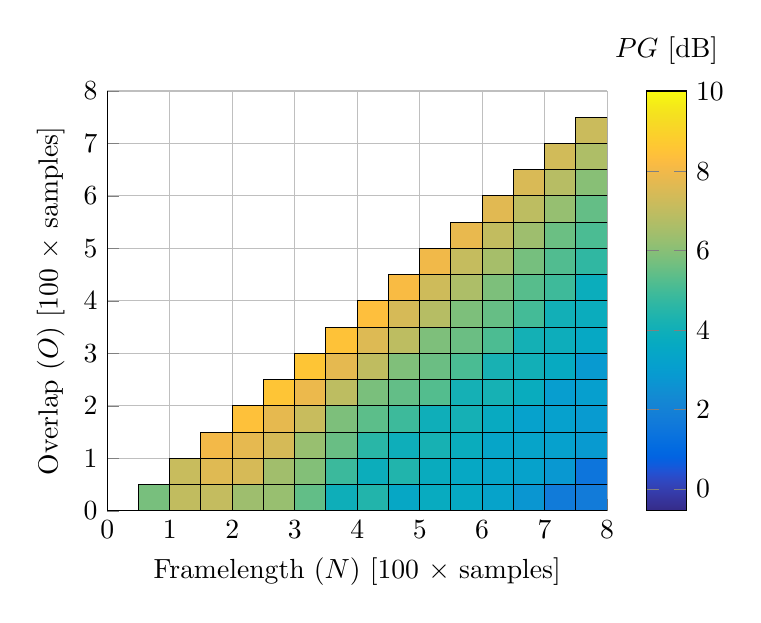
\begin{tikzpicture}

%\begin{axis}[%
%width=3.891in,
%height=3.566in,
%at={(0.653in,0.481in)},
%scale only axis,
%point meta min=0.606438537667243,
%point meta max=8.58051607966271,
%unbounded coords=jump,
%xmin=0,
%xmax=800,
%xlabel={Framelength (N) [samples]},
%xmajorgrids,
%ymin=0,
%ymax=800,
%ylabel={Overlap (O) [samples]},
%ymajorgrids,
%axis background/.style={fill=white},
%axis x line*=bottom,
%axis y line*=left,
%colormap={mymap}{[1pt] rgb(0pt)=(0.2081,0.1663,0.5292); rgb(1pt)=(0.211624,0.189781,0.577676); rgb(2pt)=(0.212252,0.213771,0.626971); rgb(3pt)=(0.2081,0.2386,0.677086); rgb(4pt)=(0.195905,0.264457,0.7279); rgb(5pt)=(0.170729,0.291938,0.779248); rgb(6pt)=(0.125271,0.324243,0.830271); rgb(7pt)=(0.0591333,0.359833,0.868333); rgb(8pt)=(0.0116952,0.38751,0.881957); rgb(9pt)=(0.00595714,0.408614,0.882843); rgb(10pt)=(0.0165143,0.4266,0.878633); rgb(11pt)=(0.0328524,0.443043,0.871957); rgb(12pt)=(0.0498143,0.458571,0.864057); rgb(13pt)=(0.0629333,0.47369,0.855438); rgb(14pt)=(0.0722667,0.488667,0.8467); rgb(15pt)=(0.0779429,0.503986,0.838371); rgb(16pt)=(0.0793476,0.520024,0.831181); rgb(17pt)=(0.0749429,0.537543,0.826271); rgb(18pt)=(0.0640571,0.556986,0.823957); rgb(19pt)=(0.0487714,0.577224,0.822829); rgb(20pt)=(0.0343429,0.596581,0.819852); rgb(21pt)=(0.0265,0.6137,0.8135); rgb(22pt)=(0.0238905,0.628662,0.803762); rgb(23pt)=(0.0230905,0.641786,0.791267); rgb(24pt)=(0.0227714,0.653486,0.776757); rgb(25pt)=(0.0266619,0.664195,0.760719); rgb(26pt)=(0.0383714,0.674271,0.743552); rgb(27pt)=(0.0589714,0.683757,0.725386); rgb(28pt)=(0.0843,0.692833,0.706167); rgb(29pt)=(0.113295,0.7015,0.685857); rgb(30pt)=(0.145271,0.709757,0.664629); rgb(31pt)=(0.180133,0.717657,0.642433); rgb(32pt)=(0.217829,0.725043,0.619262); rgb(33pt)=(0.258643,0.731714,0.595429); rgb(34pt)=(0.302171,0.737605,0.571186); rgb(35pt)=(0.348167,0.742433,0.547267); rgb(36pt)=(0.395257,0.7459,0.524443); rgb(37pt)=(0.44201,0.748081,0.503314); rgb(38pt)=(0.487124,0.749062,0.483976); rgb(39pt)=(0.530029,0.749114,0.466114); rgb(40pt)=(0.570857,0.748519,0.44939); rgb(41pt)=(0.609852,0.747314,0.433686); rgb(42pt)=(0.6473,0.7456,0.4188); rgb(43pt)=(0.683419,0.743476,0.404433); rgb(44pt)=(0.71841,0.741133,0.390476); rgb(45pt)=(0.752486,0.7384,0.376814); rgb(46pt)=(0.785843,0.735567,0.363271); rgb(47pt)=(0.818505,0.732733,0.34979); rgb(48pt)=(0.850657,0.7299,0.336029); rgb(49pt)=(0.882433,0.727433,0.3217); rgb(50pt)=(0.913933,0.725786,0.306276); rgb(51pt)=(0.944957,0.726114,0.288643); rgb(52pt)=(0.973895,0.731395,0.266648); rgb(53pt)=(0.993771,0.745457,0.240348); rgb(54pt)=(0.999043,0.765314,0.216414); rgb(55pt)=(0.995533,0.786057,0.196652); rgb(56pt)=(0.988,0.8066,0.179367); rgb(57pt)=(0.978857,0.827143,0.163314); rgb(58pt)=(0.9697,0.848138,0.147452); rgb(59pt)=(0.962586,0.870514,0.1309); rgb(60pt)=(0.958871,0.8949,0.113243); rgb(61pt)=(0.959824,0.921833,0.0948381); rgb(62pt)=(0.9661,0.951443,0.0755333); rgb(63pt)=(0.9763,0.9831,0.0538)},
%colorbar,
%colorbar style={ylabel={PG [dB]}}
%]

\begin{axis}[%
width=2.5in,
height=2.1in,
scale only axis,
point meta min=-0.551769511455843,
point meta max=10.0207598959184,
unbounded coords=jump,
xmin=0,
xmax=800,
xlabel={Framelength ($N$) [100 $\times$ samples]},
xmajorgrids,
ymin=0,
ymax=800,
ytick={0,100,...,800},
yticklabels={0,1,...,8},
xtick={0,100,...,800},
xticklabels={0,1,...,8},
ylabel={Overlap ($O$) [100 $\times$ samples]},
ymajorgrids,
axis background/.style={fill=white},
axis x line*=bottom,
axis y line*=left,
colormap={mymap}{[1pt] rgb(0pt)=(0.2081,0.1663,0.5292); rgb(1pt)=(0.211624,0.189781,0.577676); rgb(2pt)=(0.212252,0.213771,0.626971); rgb(3pt)=(0.2081,0.2386,0.677086); rgb(4pt)=(0.195905,0.264457,0.7279); rgb(5pt)=(0.170729,0.291938,0.779248); rgb(6pt)=(0.125271,0.324243,0.830271); rgb(7pt)=(0.0591333,0.359833,0.868333); rgb(8pt)=(0.0116952,0.38751,0.881957); rgb(9pt)=(0.00595714,0.408614,0.882843); rgb(10pt)=(0.0165143,0.4266,0.878633); rgb(11pt)=(0.0328524,0.443043,0.871957); rgb(12pt)=(0.0498143,0.458571,0.864057); rgb(13pt)=(0.0629333,0.47369,0.855438); rgb(14pt)=(0.0722667,0.488667,0.8467); rgb(15pt)=(0.0779429,0.503986,0.838371); rgb(16pt)=(0.0793476,0.520024,0.831181); rgb(17pt)=(0.0749429,0.537543,0.826271); rgb(18pt)=(0.0640571,0.556986,0.823957); rgb(19pt)=(0.0487714,0.577224,0.822829); rgb(20pt)=(0.0343429,0.596581,0.819852); rgb(21pt)=(0.0265,0.6137,0.8135); rgb(22pt)=(0.0238905,0.628662,0.803762); rgb(23pt)=(0.0230905,0.641786,0.791267); rgb(24pt)=(0.0227714,0.653486,0.776757); rgb(25pt)=(0.0266619,0.664195,0.760719); rgb(26pt)=(0.0383714,0.674271,0.743552); rgb(27pt)=(0.0589714,0.683757,0.725386); rgb(28pt)=(0.0843,0.692833,0.706167); rgb(29pt)=(0.113295,0.7015,0.685857); rgb(30pt)=(0.145271,0.709757,0.664629); rgb(31pt)=(0.180133,0.717657,0.642433); rgb(32pt)=(0.217829,0.725043,0.619262); rgb(33pt)=(0.258643,0.731714,0.595429); rgb(34pt)=(0.302171,0.737605,0.571186); rgb(35pt)=(0.348167,0.742433,0.547267); rgb(36pt)=(0.395257,0.7459,0.524443); rgb(37pt)=(0.44201,0.748081,0.503314); rgb(38pt)=(0.487124,0.749062,0.483976); rgb(39pt)=(0.530029,0.749114,0.466114); rgb(40pt)=(0.570857,0.748519,0.44939); rgb(41pt)=(0.609852,0.747314,0.433686); rgb(42pt)=(0.6473,0.7456,0.4188); rgb(43pt)=(0.683419,0.743476,0.404433); rgb(44pt)=(0.71841,0.741133,0.390476); rgb(45pt)=(0.752486,0.7384,0.376814); rgb(46pt)=(0.785843,0.735567,0.363271); rgb(47pt)=(0.818505,0.732733,0.34979); rgb(48pt)=(0.850657,0.7299,0.336029); rgb(49pt)=(0.882433,0.727433,0.3217); rgb(50pt)=(0.913933,0.725786,0.306276); rgb(51pt)=(0.944957,0.726114,0.288643); rgb(52pt)=(0.973895,0.731395,0.266648); rgb(53pt)=(0.993771,0.745457,0.240348); rgb(54pt)=(0.999043,0.765314,0.216414); rgb(55pt)=(0.995533,0.786057,0.196652); rgb(56pt)=(0.988,0.8066,0.179367); rgb(57pt)=(0.978857,0.827143,0.163314); rgb(58pt)=(0.9697,0.848138,0.147452); rgb(59pt)=(0.962586,0.870514,0.1309); rgb(60pt)=(0.958871,0.8949,0.113243); rgb(61pt)=(0.959824,0.921833,0.0948381); rgb(62pt)=(0.9661,0.951443,0.0755333); rgb(63pt)=(0.9763,0.9831,0.0538)},
colorbar,
colorbar style={title=$PG$ [dB]}
]%ylabel={PG}

\addplot[%
surf,
opacity = ceil(\pgfplotspointmetatransformed),
shader=flat corner,draw=black,colormap={mymap}{[1pt] rgb(0pt)=(0.2081,0.1663,0.5292); rgb(1pt)=(0.211624,0.189781,0.577676); rgb(2pt)=(0.212252,0.213771,0.626971); rgb(3pt)=(0.2081,0.2386,0.677086); rgb(4pt)=(0.195905,0.264457,0.7279); rgb(5pt)=(0.170729,0.291938,0.779248); rgb(6pt)=(0.125271,0.324243,0.830271); rgb(7pt)=(0.0591333,0.359833,0.868333); rgb(8pt)=(0.0116952,0.38751,0.881957); rgb(9pt)=(0.00595714,0.408614,0.882843); rgb(10pt)=(0.0165143,0.4266,0.878633); rgb(11pt)=(0.0328524,0.443043,0.871957); rgb(12pt)=(0.0498143,0.458571,0.864057); rgb(13pt)=(0.0629333,0.47369,0.855438); rgb(14pt)=(0.0722667,0.488667,0.8467); rgb(15pt)=(0.0779429,0.503986,0.838371); rgb(16pt)=(0.0793476,0.520024,0.831181); rgb(17pt)=(0.0749429,0.537543,0.826271); rgb(18pt)=(0.0640571,0.556986,0.823957); rgb(19pt)=(0.0487714,0.577224,0.822829); rgb(20pt)=(0.0343429,0.596581,0.819852); rgb(21pt)=(0.0265,0.6137,0.8135); rgb(22pt)=(0.0238905,0.628662,0.803762); rgb(23pt)=(0.0230905,0.641786,0.791267); rgb(24pt)=(0.0227714,0.653486,0.776757); rgb(25pt)=(0.0266619,0.664195,0.760719); rgb(26pt)=(0.0383714,0.674271,0.743552); rgb(27pt)=(0.0589714,0.683757,0.725386); rgb(28pt)=(0.0843,0.692833,0.706167); rgb(29pt)=(0.113295,0.7015,0.685857); rgb(30pt)=(0.145271,0.709757,0.664629); rgb(31pt)=(0.180133,0.717657,0.642433); rgb(32pt)=(0.217829,0.725043,0.619262); rgb(33pt)=(0.258643,0.731714,0.595429); rgb(34pt)=(0.302171,0.737605,0.571186); rgb(35pt)=(0.348167,0.742433,0.547267); rgb(36pt)=(0.395257,0.7459,0.524443); rgb(37pt)=(0.44201,0.748081,0.503314); rgb(38pt)=(0.487124,0.749062,0.483976); rgb(39pt)=(0.530029,0.749114,0.466114); rgb(40pt)=(0.570857,0.748519,0.44939); rgb(41pt)=(0.609852,0.747314,0.433686); rgb(42pt)=(0.6473,0.7456,0.4188); rgb(43pt)=(0.683419,0.743476,0.404433); rgb(44pt)=(0.71841,0.741133,0.390476); rgb(45pt)=(0.752486,0.7384,0.376814); rgb(46pt)=(0.785843,0.735567,0.363271); rgb(47pt)=(0.818505,0.732733,0.34979); rgb(48pt)=(0.850657,0.7299,0.336029); rgb(49pt)=(0.882433,0.727433,0.3217); rgb(50pt)=(0.913933,0.725786,0.306276); rgb(51pt)=(0.944957,0.726114,0.288643); rgb(52pt)=(0.973895,0.731395,0.266648); rgb(53pt)=(0.993771,0.745457,0.240348); rgb(54pt)=(0.999043,0.765314,0.216414); rgb(55pt)=(0.995533,0.786057,0.196652); rgb(56pt)=(0.988,0.8066,0.179367); rgb(57pt)=(0.978857,0.827143,0.163314); rgb(58pt)=(0.9697,0.848138,0.147452); rgb(59pt)=(0.962586,0.870514,0.1309); rgb(60pt)=(0.958871,0.8949,0.113243); rgb(61pt)=(0.959824,0.921833,0.0948381); rgb(62pt)=(0.9661,0.951443,0.0755333); rgb(63pt)=(0.9763,0.9831,0.0538)},mesh/rows=16]
table[row sep=crcr, point meta=\thisrow{c}] {%
%
x	y	c\\
50	0	5.75681405370928\\
50	50	nan\\
50	100	nan\\
50	150	nan\\
50	200	nan\\
50	250	nan\\
50	300	nan\\
50	350	nan\\
50	400	nan\\
50	450	nan\\
50	500	nan\\
50	550	nan\\
50	600	nan\\
50	650	nan\\
50	700	nan\\
50	750	nan\\
100	0	7.02872386820369\\
100	50	7.16320561320949\\
100	100	nan\\
100	150	nan\\
100	200	nan\\
100	250	nan\\
100	300	nan\\
100	350	nan\\
100	400	nan\\
100	450	nan\\
100	500	nan\\
100	550	nan\\
100	600	nan\\
100	650	nan\\
100	700	nan\\
100	750	nan\\
150	0	7.07141543931447\\
150	50	7.62166199870556\\
150	100	8.04478981508383\\
150	150	nan\\
150	200	nan\\
150	250	nan\\
150	300	nan\\
150	350	nan\\
150	400	nan\\
150	450	nan\\
150	500	nan\\
150	550	nan\\
150	600	nan\\
150	650	nan\\
150	700	nan\\
150	750	nan\\
200	0	6.36367548725126\\
200	50	7.45043065691566\\
200	100	7.76985455573913\\
200	150	8.43045234663355\\
200	200	nan\\
200	250	nan\\
200	300	nan\\
200	350	nan\\
200	400	nan\\
200	450	nan\\
200	500	nan\\
200	550	nan\\
200	600	nan\\
200	650	nan\\
200	700	nan\\
200	750	nan\\
250	0	6.2747518539513\\
250	50	6.43177618340764\\
250	100	7.41748637065385\\
250	150	7.78032261424947\\
250	200	8.56548684977141\\
250	250	nan\\
250	300	nan\\
250	350	nan\\
250	400	nan\\
250	450	nan\\
250	500	nan\\
250	550	nan\\
250	600	nan\\
250	650	nan\\
250	700	nan\\
250	750	nan\\
300	0	5.44672828482622\\
300	50	5.93228217654232\\
300	100	6.27730322097317\\
300	150	7.16869699988956\\
300	200	7.90513810271794\\
300	250	8.58051607966271\\
300	300	nan\\
300	350	nan\\
300	400	nan\\
300	450	nan\\
300	500	nan\\
300	550	nan\\
300	600	nan\\
300	650	nan\\
300	700	nan\\
300	750	nan\\
350	0	3.96082759661116\\
350	50	4.87443490181049\\
350	100	5.54559386716673\\
350	150	5.84219216027062\\
350	200	6.94721738777555\\
350	250	7.74501762599016\\
350	300	8.47753650611538\\
350	350	nan\\
350	400	nan\\
350	450	nan\\
350	500	nan\\
350	550	nan\\
350	600	nan\\
350	650	nan\\
350	700	nan\\
350	750	nan\\
400	0	4.42621008095804\\
400	50	3.89426906544824\\
400	100	4.56352235440709\\
400	150	5.36296065670868\\
400	200	5.78832093933364\\
400	250	6.9866185309537\\
400	300	7.59713514794527\\
400	350	8.36055209221641\\
400	400	nan\\
400	450	nan\\
400	500	nan\\
400	550	nan\\
400	600	nan\\
400	650	nan\\
400	700	nan\\
400	750	nan\\
450	0	3.50354221368119\\
450	50	4.40681513298228\\
450	100	3.95685694859008\\
450	150	4.9042385635657\\
450	200	5.4633728598898\\
450	250	5.88326157594826\\
450	300	6.94594934868294\\
450	350	7.44676002191824\\
450	400	8.19574813733794\\
450	450	nan\\
450	500	nan\\
450	550	nan\\
450	600	nan\\
450	650	nan\\
450	700	nan\\
450	750	nan\\
500	0	3.72835292601718\\
500	50	3.78107635637919\\
500	100	4.18031741794866\\
500	150	3.96907831408446\\
500	200	5.24334000720054\\
500	250	5.57020508886556\\
500	300	5.84956274795864\\
500	350	6.81670541965121\\
500	400	7.27827902100581\\
500	450	8.01587600126447\\
500	500	nan\\
500	550	nan\\
500	600	nan\\
500	650	nan\\
500	700	nan\\
500	750	nan\\
550	0	3.55899161331985\\
550	50	3.5627092998632\\
550	100	3.83378904045391\\
550	150	4.12408113752203\\
550	200	4.12592880853361\\
550	250	5.10843403805551\\
550	300	5.57168633048741\\
550	350	5.8397995836529\\
550	400	6.63314311215868\\
550	450	7.10066891370851\\
550	500	7.84156609258604\\
550	550	nan\\
550	600	nan\\
550	650	nan\\
550	700	nan\\
550	750	nan\\
600	0	3.28411067048159\\
600	50	3.40775040817206\\
600	100	3.38318838169599\\
600	150	3.68526563556863\\
600	200	4.14960399353065\\
600	250	4.19614482309243\\
600	300	5.14142197703852\\
600	350	5.5090628438645\\
600	400	5.83359225300751\\
600	450	6.51328417187561\\
600	500	7.03962308152776\\
600	550	7.67867879226025\\
600	600	nan\\
600	650	nan\\
600	700	nan\\
600	750	nan\\
650	0	2.74376613648247\\
650	50	3.23740097468862\\
650	100	3.32831923922301\\
650	150	3.21486571971626\\
650	200	3.78488209774861\\
650	250	4.04389848517578\\
650	300	4.12062294067197\\
650	350	5.01568199288583\\
650	400	5.30306339600344\\
650	450	5.73133270755829\\
650	500	6.37102277513149\\
650	550	6.93506594122197\\
650	600	7.50728208572552\\
650	650	nan\\
650	700	nan\\
650	750	nan\\
700	0	1.70836217458545\\
700	50	2.78412983405078\\
700	100	3.1621221086197\\
700	150	3.16115206951762\\
700	200	3.03102270121495\\
700	250	3.66346881127579\\
700	300	3.90010259938533\\
700	350	4.04738561235305\\
700	400	4.92042209157116\\
700	450	5.20934705417486\\
700	500	5.58370749982053\\
700	550	6.23469505199079\\
700	600	6.82628236008956\\
700	650	7.34941945405539\\
700	700	nan\\
700	750	nan\\
750	0	1.74688922906691\\
750	50	1.48355051040994\\
750	100	2.87849169061716\\
750	150	2.90386747913936\\
750	200	3.09480417856087\\
750	250	2.88874071124512\\
750	300	3.57777233418346\\
750	350	3.84248224292264\\
750	400	3.85437738806347\\
750	450	4.69299998602383\\
750	500	5.12825272160081\\
750	550	5.47698500020064\\
750	600	6.00913351283639\\
750	650	6.66749521550333\\
750	700	7.19103585642779\\
750	750	nan\\
800	0	0.606438537667243\\
800	50	1.7701782237956\\
800	100	1.1545148340565\\
800	150	2.86295949584776\\
800	200	2.88822591275756\\
800	250	3.06012747568978\\
800	300	2.78286049390807\\
800	350	3.49244238740902\\
800	400	3.91706255141676\\
800	450	3.90881912203657\\
800	500	4.55170464947537\\
800	550	4.95690649177466\\
800	600	5.4247931683094\\
800	650	5.88695032583024\\
800	700	6.4885402905689\\
800	750	7.03631961801922\\
};
\end{axis}
\end{tikzpicture}%}
%		\end{column}
%	\end{columns}
%\end{frame}


%\subsection{Prediction}
%\begin{frame}{This is christians part}{some fancy subtitle}		
%	\begin{columns}
%		\begin{column}{0.5\textwidth}
%			fish can be both blue and green	
%		\end{column}
%		\begin{column}{0.5\textwidth} 
%			\begin{itemize}
%				\item<1-> Blue fish
%				\item<2-> Green fish
%				\item<3-> But can we neglect the purple fish?
%				\begin{itemize}
%					\item<4-> Yes, because they are gay
%				\end{itemize}			
%			\end{itemize}		
%		\end{column}
%	\end{columns}
%\end{frame}